%\documentclass[a4paper,12pt]{report}
%\documentclass[a4paper,11pt]{book}
\documentclass[a4paper,11pt]{scrbook}
\usepackage{preamble}

% include  book references
\usepackage{xr-hyper}
\externaldocument{book}

\usepackage{bigfoot}
% \DeclareNewFootnote{default} % if `normal' footnotes should be printed first
\DeclareNewFootnote{solution}
\renewcommand\thefootnotesolution{}

%\renewcommand\exsheetsprintsolution[2]{\footnotesolution{#1#2}}
% \renewcommand\exsheetsprintsolution[2]{
% \footnotesolution{
% \ExSheetsHeading
%   {runin}               % headings style
%   {Hint}                % heading
%   {\GetQuestionProperty{counter}{\CurrentQuestionID}}% number
%   {0}                   % points -- need to be zero here
%   {0}                   % bonus points -- need to be zero here
%   {\CurrentQuestionID}%                % ID
% \GetQuestionProperty{hint}{\CurrentQuestionID}%
% #1#2
% }
% }

\renewcommand\exsheetsprintsolution[2]{
\ExSheetsHeading
{runin}               % headings style
{Hint}                % heading
{\GetQuestionProperty{counter}{\CurrentQuestionID}}% number
{0}                   % points -- need to be zero here
{0}                   % bonus points -- need to be zero here
{##1}%                % ID
\GetQuestionProperty{hint}{\CurrentQuestionID}
#1#2
}
\renewcommand{\hint}[1]{\SetQuestionProperties{ hint = {#1}}}


\SetupExSheets{
  headings = runin,
  question/print = true,
  solution/print = true,
  counter-within = section,
  counter-format = ch.se.qu
}


\begin{document}


%\include{organization}
%\chapter{Introduction}\label{sec:introduction}
%\addcontentsline{toc}{chapter}{Introduction}

\paragraph{Motivation and Examples}
Queueing systems abound, and the analysis and control of queueing
systems are major topics in the control, performance evaluation and
optimization of production and service systems. 


At my local supermarket, for instance, any customer that joins a queue
of 4 of more customers get his/her shopping for free. Of course, there
are some constraints: at least one of the cashier facilities has to
unoccupied by a server and the customers in queue should be equally
divided over the cashiers that are open. (And perhaps there are some
further rules, of which I am unaware.) The manager that controls the
occupation of the cashier positions is focused on keeping
$\pi(4)+\pi(5)+\cdots$, i.e., the fraction of customers that see upon
arrival a queue length exceeding~3, very small. In a sense,
this is easy enough: just hire many cashiers. However, the cost of
personnel may then outweigh the yearly average cost of paying the
customer penalties. Thus, the manager's problem becomes to plan and
control the service capacity  in such a way that both
the penalties and the personnel cost are small.

Fast food restaurants also deal with many interesting queueing
situations. Consider, for instance, the making of
hamburgers. Typically, hamburgers are made-to-stock, in other words,
they are prepared before the actual demand has arrived. Thus, hamburgers
in stock can be interpreted as customers in queue waiting for service,
where the service time is the time between the arrival of two
customers that buy hamburgers. The hamburgers have a typical lifetime,
and they have to be scrapped if they remain on the shelf longer than
some amount of time. Thus, the waiting time of hamburgers has to be
closely monitored. Of course, it is easy to achieve zero scrap cost,
simply by keeping no stock at all.  However, to prevent lost-sales it
is very important to maintain a certain amount of hamburgers on
stock. Thus, the manager has to balance the scrap cost against the
cost of lost sales. In more formal terms, the problem is to choose a
policy to prepare hamburgers such that the cost of excess waiting time
(scrap) is balanced against the cost of an empty queue (lost sales).

Service systems, such as hospitals, call centers, courts, and so on,
have a certain capacity available to serve customers. The performance
of such systems is, in part, measured by the total number of jobs
processed per year and the fraction of jobs processed within a certain
time between receiving and closing the job. Here the problem is to
organize the capacity such that the sojourn time, i.e., the typical
time a job spends in the system, does not exceed some threshold, and
such that the system achieves a certain throughput, i.e., jobs served
per year. 

Clearly, all the above systems can be seen as queueing systems that
have to be monitored and controlled to achieve a certain
performance. The performance analysis of such systems can, typically,
be characterized by the following performance measures:
\begin{enumerate}
\item The fraction of time $p(n)$ that the system contains $n$
  customers. In particular, $1-p(0)$, i.e., the fraction of time the
  system contains jobs, is important, as this is a measure of the
  time-average occupancy of the servers, hence related to personnel
  cost.
\item The fraction of customers $\pi(n)$ that `see upon arrival' the
  system with $n$ customers. This measure relates to customer
  perception and lost sales, i.e., fractions of arriving customers
  that do not enter the system.
\item The average, variance, and/or distribution of the waiting time.
\item The average, variance, and/or distribution of the number of customers in the system.\
\end{enumerate}
Here the system can be anything that is capable of holding jobs, such
as a queue, the server(s), an entire court house, patients waiting for
an MRI scan in a hospital, and so on.

It is important to realize that a queueing system can, typically, be
decomposed into \emph{two subsystems}, the queue itself and the
service system. Thus, we are concerned with three types of waiting:
waiting in queue, i.e., \emph{queueing time}, waiting while being in
service, i.e., the \emph{service time}, and the total waiting time in
the system, i.e., the \emph{sojourn time}.

\paragraph{Organization}


In these notes we will be primarily concerned with making models of
queueing systems such that we can compute or estimate the above
performance measures.  Part of our work is to derive analytic
models. The benefit of such models is that they offer structural
insights into the behavior of the system and scaling laws, such as
that the average waiting time scales (more or less) linearly in the
variance of the service times of individual customers. However, these
models have severe shortcomings when it comes to analyzing real
queueing systems, in particular when particular control rules have to
be assessed.  Consider, for example, the service process at a check-in
desk of KLM. Business customers and economy customers are served by
two separate queueing systems. The business customers are served by
one server, server A say, while the economy class customers by three
servers, say. What would happen to the sojourn time of the business
customers if server A would be allowed to serve economy class
customers when the business queue is empty? For the analysis of such
cases simulation is a very useful and natural approach.

In the first part of these notes we concentrate on the analysis of
\emph{sample paths of a queueing process}. We assume that a typical
sample path captures the `normal' stochastic behavior of the
system. This sample-path approach has two advantages. In the first
place, most of the theoretical results follow from very concrete
aspects of these sample paths. Second, the analysis of sample-paths
carries over right away to simulation. In fact, simulation of a
queueing system offers us one (or more) sample paths, and based on
such sample paths we derive behavioral and statistical properties of
the system. Thus, the performance measures defined for sample paths
are precisely those used for simulation.  

Our aim is not to provide rigorous proofs for all results derived below; for this we refer to
\cite{el-taha98:_sampl_path_analy_queuein_system}. As a consequence we tacitly
assume in the remainder that results derived from the (long-run)
analysis of a particular sample path are equal to their `probabilistic
counterpart'. 
% For instance, assume that the sequence of service times
% $S_1, S_2, \ldots$ for jobs $1, 2, \ldots$, are i.i.d., i.e.,
% independent and identically distributed. It then follows from the
% strong law of large numbers that $k^{-1}\sum_{i=1}^k S_i \to \E S$,
% almost surely, where $\E S$ is the expectation of a generic service
% time $S$ with the same distribution as the service times
% $\{S_i\}$. While this is already a quite deep result in probability
% theory, the problems become much harder when we have to consider the
% sequence of waiting times $\{W_i\}$. As we will see later, the times
% are constructed in terms of recursions, and are \emph{not}
% i.i.d. Thus, we cannot right away apply the strong law to conclude
% that results of sample path analysis capture the long-run
% probabilistic behavior the waiting time. However, intuitively, it is
% hopefully clear that the sequence of waiting times $W_i$ will
% converge, in some sense, to a random variable $W$ and that the
% stochastic properties of $W$ can be obtained from a sample-path
% analysis of the waiting times $\{W_i\}$. In the remainder we will
% freely use that $k^{-1}\sum_{i=1}^k W_i \to \E W$ as $k\to\infty$, and
% so on.

In the second part of these notes we construct algorithms to analyze open and closed
queueing networks. Many of the sample path results developed for the
single-station case can be applied to these networks. As such, theory,
simulation and algorithms form a nicely round out part of work.  For
this part we refer to the book of Prof. Zijm; the present set of notes
augments the discussion there.


\paragraph{Exercises}

I urge you to make \emph{all} exercises in this set of notes. The main text contains hardly any examples or derivations: the exercises  \emph{illustrate} the material and force you to \textit{think} about the technical parts. The
exercises require many of the tools you learned previously in courses
on calculus, probability, and linear algebra. Here you can see them
applied. Moreover, many of these tools will be useful for other,
future, courses. Thus, the investments made here will pay off for the
rest of your (student) career. 

You'll notice that many of these problems are quite difficult, often
not because the problem itself is difficult, but because you need to
combine a substantial amount of knowledge all at the same time.  All
this takes time and effort. Realize that the 
exercises are not intended to be  easy (otherwise we could have been satisfied with computing $1+1$). The problems should be doable, but hard.

The solution manual is meant to prevent you from getting stuck and to
help you increase your knowledge of probability, linear algebra,
programming (analysis with computer support), and queueing in
particular. Thus, read the solutions very carefully. 

As a guideline to making the exercises I recommend the following
approach.  First read the notes. Then attempt to make a exercises for
10 minutes or so by yourself. If by that time you have not obtained a
good idea on how to approach the problem, check the solution
manual. Once you have understood the solution, try to repeat the
arguments \emph{with the solution manual closed}.

% \paragraph{Symbols}

% The meaning of the symbols in the margin of pages are as follows:
% \begin{itemize}
% \item The symbol \recall{} in the margin means that you have to
%   memorize the \emph{emphasized concepts}.
% \item The symbol \hintsymbol in the margin means that this question
%   has a \emph{hint}.
% \item The symbol \tbd in the margin means that this question or its
%   solution requires still some \emph{work on my part}; you can skip
%   it.
% \end{itemize}

\paragraph{Further reading}

The following books are very useful to extend one's knowledge of probability theory and queueing systems:
\begin{enumerate}
\item \citet{capinski03:_probab_probl}
\item \citet{tijms94:_stoch_model_algor_approac} and/or \citet{tijms03:_first_cours_stoch_model}
\item \citet{el-taha98:_sampl_path_analy_queuein_system}
\item \citet{bolch06:_queuein_networ_markov_chain}
\end{enumerate}

\paragraph{Acknowledgments}

I would like to acknowledge dr. J.W. Nieuwenhuis for our many
discussions on the formal aspects of queueing theory and
prof. dr. W.H.M. Zijm for allowing me to use the first few chapters of
his book. 

\clearpage

%Finally, we use the terms `jobs' and `customers' interchangeably.



\chapter{Single-Station Queueing Systems}
%\input{todo/appendix.tex}
%In this chapter, we start with a discussion of the exponential
distribution and the related Poisson process, as these concepts are
perhaps the most important building blocks of queueing theory. With
these concepts we can specify the arrival and service processes of
customers, so that we can construct queueing processes and define
performance measures to provide insight into the (transient and
average) behavior of queueing processes. As it turns out, these
constructions can be easily implemented as computer programs, thereby
allowing to use simulation to analyze queueing systems. We then
continue with developing models for various single-station queueing
systems in steady-state, which is, in a sense to be discusses later,
the long-run behavior of a stochastic system.\footnote{This statement
is, admittedly, vague, to say the least.} In the analysis we use
sample-path arguments to count how often certain events occur as
functions of time. Then we define probabilities in terms of limits of
fractions of these counting processes. Another useful aspect of
sample-path analysis is that the definitions for the performance
measures are entirely constructive, hence by leaving out the limits,
they provide expressions that can be right away used in statistical
analysis of (simulations of) queueing systems. Level-crossing
arguments will be of particular importance as we use these time and
again to develop recursions by which we can compute steady-state
probabilities of the queue length or waiting time process.



%\section{Exponential Distribution}
\label{sec:expon-distr}


\subsection*{Theory and Exercises}

\Opensolutionfile{hint}
\Opensolutionfile{ans}

In the previous section we introduced the Poisson process as a natural model of the number of jobs arriving in during intervals of time.  As we will see in the sections to come, the modeling and analysis of any queueing system is typically easier if we specificy  the (probability)
distribution of the interarrival times, i.e., the time between consecutive arrival epochs of jobs.
A particular fruitful model for the distribution of the interarrival times is the exponential distribution. Here we show how this relates to the Poisson distribution,  and we also derive many useful general probability concepts and apply these to the exponential distribution.  Then we use simulation to provide yet further movivation for the use of the exponential distribution as a useful model for interarrival times of customers.

Let us assume that the interarrival times form a sequence $\{X_i\}$ of \recall{independent and identically distributed  (i.i.d.)}  random variables, and let us write $X$ for the generic
random time between two successive arrivals. For many queueing
systems, measurements of the interarrival times between consecutive
arrivals show that it is reasonable to model an interarrival $X$ as
an \recall{exponentially distributed} random variable, i.e.,
\begin{equation*}
  \P{X \leq t} = 1- e^{-\lambda t}
\end{equation*}
Moreover,  the exponential distribution  derives directly from the Poisson distribution. Observe that, if there are no arrivals in some interval $[0,t]$, then it
must be that $N(t) = 0$. Hence, the first interarrival time $X$, i.e., the time until the first customer,  must be larger than $t$.  Therefore,
\begin{equation*}
 \P{X1> t} = \P{N(t) = 0} = e^{-\lambda t} \frac{(\lambda t)^0}{0!}= e^{-\lambda t}.
\end{equation*}
Recall that the constant $\lambda$ is called the arrival
\recall{rate}.  

In the sequel we often write $X\sim \exp(\lambda)$ to
mean that~$X$ is exponentially distributed with rate~$\lambda$.



\begin{exercise} 
In the above expression for $\P{X\leq t}$ we require that $\lambda>0$. What would happen if you would allow $\lambda$ to be zero or negative?
\begin{hint}
  The interpretation of the function $1-e^{-\lambda t}$ is a probability. What are the consequences of this? What happens if $\lambda=0$?
\end{hint}
\begin{solution}
  If $\lambda<0$, then $1-e^{-\lambda t}$ grows to $-\infty$ if $t\to \infty$. Just by itself this is not a problem. However, in our case $1-e^{-\lambda t}$ has the interpretation of a distribution function. Now, recall that a distribution function is bounded to values in the interval $[0,1]$.

Suppose $\lambda=0$. Then $\P{X\leq t} = 1-e^{0} = 0$. In words, this would mean that the probability of a finite interarrival time between any two customers is zero. So, no customers can arrive in this case. 
\end{solution}
\end{exercise}

\begin{exercise} \label{exer:lambda}
  If the random variable $X\sim\exp(\lambda)$, show that its mean $\E X = \frac{1}\lambda$. Interpret this result.
  \begin{hint}
 \begin{equation*}
    \E X = \int_0^\infty t f(t)\, \d t =
    \int_0^\infty t \lambda e^{-\lambda t}\, \d t 
  \end{equation*}
  where~$f(t)=\lambda e^{-\lambda t}$ is the density function of the distribution function $F$ of $X$. Now solve the integral.
  \end{hint}
  \begin{solution}
    \begin{align*}
\E{X} 
&= \int_0^\infty t \lambda e^{-\lambda t} \d t, \quad\text{density is } \lambda e^{-\lambda t} \\
&=   \lambda^{-1} \int_0^\infty u e^{-u}\, \d u, \quad \text{ by  change of variable $u=\lambda t$},   \\
&=  -\lambda^{-1}\left. t e^{- t}\right|_0^\infty + \lambda^{-1} \int_0^\infty e^{- t} \d t\\
&=  - \lambda^{-1} \left. e^{- t} \right|_0^\infty =  \frac1\lambda.
    \end{align*}

For the interpretation, if jobs arrive at rate $\lambda$, the average time between two arrivals is $\lambda^{-1}$.
  \end{solution}
\end{exercise}


\begin{exercise}\label{ex:15} 
  If $X\sim\exp(\lambda)$, show that its second moment $\E{X^2} =  \frac{2}{\lambda^2}$.
  \begin{hint}
  \begin{equation*}
  \E{X^2}= \int_0^\infty t^2 \lambda e^{-\lambda t}\, \d t =  \frac{2}{\lambda^2}.
  \end{equation*}
  \end{hint}
  \begin{solution}
    \begin{align*}
\E{X^2} 
&= \int_0^\infty t^2 \lambda e^{-\lambda t} \d t \\
&=   \lambda^{-2} \int_0^\infty u^2 e^{-u}\, \d u, \quad \text{ by  change of variable $u=\lambda t$},   \\
&= -\lambda^{-2}\left. t^2 e^{- t}\right|_0^\infty + 2\lambda^{-2}\int_0^\infty t e^{- t} \d t \\
&=  -2\lambda^{-2}\left. t e^{- t}\right|_0^\infty + 2\lambda^{-2} \int_0^\infty e^{- t} \d t\\
&=  - 2\lambda^{-2} \left. e^{- t} \right|_0^\infty \\
&=  2/\lambda^2.
    \end{align*}
  \end{solution}
\end{exercise}


\begin{exercise} 
  If $X\sim\exp(\lambda)$, show that the \recall{variance}
$\V X = \lambda^{-2}$.
  \begin{hint} Use, and memorize, the very practical formula
  \begin{equation*}
  \V X = \E X^2 - (\E X)^2.
  \end{equation*}
  \end{hint}
  \begin{solution}
    By the previous problems, $\E{X^2}=2/\lambda^2$ and $\E X = 1/\lambda$. 
  \end{solution}
\end{exercise}

The  above exercises can also be easily solved with the moment generating function of $X\geq 0$
\begin{equation*}
  M_X(t) = \E{e^{tX}} = \int_0^\infty e^{tx} \lambda e^{-\lambda x} \d x.
\end{equation*}

\begin{exercise}
Why do we require that $t \in [0, \lambda)$ in the definition of $M_X(t)$?
\begin{solution}
\begin{equation*}
  M_X(t) = \E{e^{tX}} = \lambda \int_0^\infty e^{-(\lambda-t) x}\d x.
\end{equation*}
  If $t - \lambda>0$, then this integral becomes $\infty$. 
\end{solution}
\end{exercise}

\begin{exercise}
  What is $M_X(0)?$
  \begin{solution}
    $M_X(0) = \E{e^{0 X}} = \E{e^0} = \E{1} = 1$
  \end{solution}
\end{exercise}

\begin{exercise}\label{ex:33}
 If $X$ is an exponentially distributed random variable with
    parameter $\lambda$, show that its moment generating function
    \begin{equation*}
    M_X(t) = \frac{\lambda}{\lambda-t}.
    \end{equation*}
   \begin{hint}
    \begin{equation*}
      M_X(t) = \E{\exp(t X)} =\int_0^\infty e^{tx} f(x) \,\d x.
\end{equation*}
\end{hint}
    \begin{solution}
    \begin{align*}
      M_X(t) &= \E{\exp(t X)}  
=\int_0^\infty e^{tx} f(x) \,\d x 
=\int_0^\infty e^{tx} \lambda e^{-\lambda x} \,\d x  \\
&=\lambda \int_0^\infty e^{(t-\lambda)x} \,\d x 
=\frac{\lambda}{\lambda -t}.
    \end{align*}
    \end{solution}
  \end{exercise}

\begin{exercise}
    Use the moment generating function to show that 
    \begin{align*}
      \E{X} &=\frac1\lambda, & 
      \E{X^2} &=\frac2{\lambda^2}.
    \end{align*}
\begin{hint}
    \begin{align*}
      \E{X} &= M_X'(0) &  \E{X^2} &= M_X''(0).
    \end{align*}
where $M'(t) = \frac{\d}{\d t} M(t)$. 
\end{hint}
\begin{solution}
  $\E X = M_X'(0)=\lambda/(\lambda-t)^2$. Hence, $M_X'(0)=1/\lambda$. And, $\E{X^2} = M_X''(t)=2\lambda/(\lambda-t)^3$, hence $\E{X^2}=M_X''(0)=2\lambda/\lambda^3=2\lambda^{-2}$. 
\end{solution}
  \end{exercise}

\begin{exercise}
  Prove that the square coefficient of variation (SCV) of $X$ is $C^2 =1$.  
\begin{solution}
  By the previous problems, $\V X = 1/\lambda^2$ and $\E X=1/\lambda$.
\end{solution}
\end{exercise}


Let us now show with simulation how the exponential distribution
originates. Consider $N$ people that regularly visit a shop. We assume
that we can characterize the interarrival times
$\{X_k^i, k=1,2, \ldots\}$ of customer $i$ by some distribution
function, for instance the uniform distribution. Then, with
$A_{0}^i=0$ for all~$i$, define 
\begin{equation}\label{eq:A_kk}
A_k^i = A_{k-1}^i + X_k^i = \sum_{j=1}^k X_j^i,
\end{equation}
as the arrival moment of the $k$th visit of customer $i$.  Now the
shop owner `sees' the superposition of the arrivals of all
customers. One way to compute the arrival moments of all customers
together is to put all the arrival times
$\{A_k^i, k=1,\ldots,n, i=1,\ldots,N\}$ into one set, and sort these
numbers in increasing order. This results in the (sorted) set of
arrival times $\{A_k, k=1,2,\ldots\}$ at the shop of all customers together. Taking $A_0=0$,  then
\begin{equation}\label{eq:X_kk}
X_k = A_k - A_{k-1},
\end{equation}
must be the interarrival time between the $k-1$th and
$k$th customer at the shop.  Thus, with this procedure, starting from interarrival times of
individual customers, we can construct interarrival times as seen by
the shop.


Suppose that we  generate, by means of simulation, many interarrival times for a set of individual customers, compute the arrival times by~(\ref{eq:A_kk}), sort these, and compute with~(\ref{eq:X_kk}) the interarrival times $\{X_k\}$ of customers as seen by the shop.  To plot the \recall{empirical distribution function}, or the \emph{histogram}, of $\{X_k\}$, we just  count the
number of interarrival times smaller than time $t$ for any $t$.  Then the emperical distribution of $\{X_k\}$ is defined as
\begin{equation*}
  \P{X \leq t}_{n} = \frac1{n}\sum_{k=1}^{n} \1{X_k\leq t},
\end{equation*}
where the \emph{indicator function} is $\1{X_k\leq t}=1$ if $X_k\leq t$ and $\1{X_k\leq t}=0$
if $X_k> t$.  

Let us now compare the probability density as
obtained for several simulation scenarios to the density of the
exponential distribution, i.e., to $\lambda e^{-\lambda t}$.  As a
first example, take $N=1$ customer and let the computer generate
$n=100$ uniformly distributed numbers on the set $[4, 6]$.  Thus, the
time between two visits of this customer is somewhere between $4$ and
$6$ hours, and the average interarrival times $\E X = 5$. In a second
simulation we take $N=3$ customers, and in the third, $N=10$
customers. 

The emperical distributions are shown, from left to right,
in the three panels in Figure~\ref{fig:uniformfew}. The continuous
curve is the graph of $\lambda e^{-\lambda x}$ where
$\lambda = N/\E X = N/5$. (Recall from Exercise~(\ref{exer:lambda}) that when $1$
person visits the shop  with an average interarrival time of $5$
hours,  the arrival rate is $1/5$. Hence, when $N$ customers visit the shop, each with an average interarrival time of 5 hours, the total arrival rate as seen by the shop must be $N/5$.)  


\begin{figure}[ht]
  \centering
  \begin{tabular}[h]{c}
% see progs/convergence_to_exp.py
 % This file was created by matplotlib2tikz v0.5.15.
\begin{tikzpicture}

\begin{groupplot}[group style={group size=3 by 1}]
\nextgroupplot[
title={$N=1, n=100, b=10$},
xmin=0, xmax=8,
ymin=0, ymax=2,
width=5cm,
height=5cm,
tick align=outside,
xmajorgrids,
x grid style={white},
ymajorgrids,
y grid style={white},
axis line style={white},
axis background/.style={fill=white!89.803921568627459!black},
legend entries={{simulation},{theory}},
legend cell align={left},
legend style={draw=white!80.0!black, fill=white!89.803921568627459!black}
]
\addplot [semithick, black, mark=*, mark size=1, mark options={solid}, only marks]
table {%
4.14316511876391 0.477456921988451
4.33356782678306 0.530507691098278
4.52397053480221 0.74271076753759
4.71437324282137 0.424406152878623
4.90477595084052 0.636609229317934
5.09517865885968 0.583558460208106
5.28558136687883 0.583558460208106
5.47598407489798 0.583558460208106
5.66638678291714 0.212203076439311
5.85678949093629 0.477456921988451
};
\addplot [semithick, black]
table {%
0 0.201666243229445
0.1 0.197640049681036
0.2 0.193694237629449
0.3 0.189827202287196
0.4 0.18603737090579
0.5 0.182323202136099
0.6 0.178683185401466
0.7 0.175115840283355
0.8 0.171619715919244
0.9 0.168193390412562
1 0.164835470254385
1.1 0.16154458975669
1.2 0.158319410496923
1.3 0.15515862077365
1.4 0.152060935073083
1.5 0.149025093546251
1.6 0.14604986149661
1.7 0.143134028877887
1.8 0.140276409801946
1.9 0.137475842056476
2 0.134731186632315
2.1 0.132041327260207
2.2 0.129405169956808
2.3 0.126821642579754
2.4 0.124289694391617
2.5 0.12180829563256
2.6 0.119376437101529
2.7 0.116993129745803
2.8 0.114657404258743
2.9 0.112368310685563
3 0.110124918036983
3.1 0.107926313910584
3.2 0.105771604119734
3.3 0.103659912329913
3.4 0.101590379702301
3.5 0.0995621645444846
3.6 0.0975744419681357
3.7 0.0956264035535224
3.8 0.0937172570207203
3.9 0.0918462259073866
4 0.0900125492529686
4.1 0.0882154812892152
4.2 0.0864542911368687
4.3 0.084728262508411
4.4 0.0830366934167454
4.5 0.0813788958896931
4.6 0.0797541956901909
4.7 0.0781619320420749
4.8 0.0766014573613375
4.9 0.0750721369927518
5 0.0735733489517529
5.1 0.0721044836714721
5.2 0.0706649437548231
5.3 0.0692541437315359
5.4 0.0678715098200426
5.5 0.0665164796941166
5.6 0.0651885022541708
5.7 0.063887037403122
5.8 0.0626115558267297
5.9 0.0613615387783206
6 0.060136477867811
6.1 0.0589358748549412
6.2 0.0577592414466378
6.3 0.0566060990984221
6.4 0.0554759788197825
6.5 0.0543684209834333
6.6 0.0532829751383812
6.7 0.0522191998267238
6.8 0.051176662404106
6.9 0.0501549388637608
7 0.0491536136640626
7.1 0.048172279559524
7.2 0.0472105374351664
7.3 0.0462679961441972
7.4 0.0453442723489281
7.5 0.0444389903648687
7.6 0.0435517820079337
7.7 0.0426822864446998
7.8 0.0418301500456523
7.9 0.0409950262413616
};
\nextgroupplot[
title={$N=3, n=100, b=10$},
xmin=0, xmax=8,
ymin=0, ymax=2,
width=5cm,
height=5cm,
tick align=outside,
xmajorgrids,
x grid style={white},
ymajorgrids,
y grid style={white},
axis line style={white},
axis background/.style={fill=white!89.803921568627459!black},
legend entries={{simulation},{theory}},
legend cell align={left},
legend style={draw=white!80.0!black, fill=white!89.803921568627459!black}
]
\addplot [semithick, black, mark=*, mark size=1, mark options={solid}, only marks]
table {%
0.270772192547602 0.495388011520489
0.804119872907879 0.344890387767429
1.33746755326816 0.232017169952634
1.87081523362843 0.169309826722192
2.40416291398871 0.144226889430016
2.93751059434898 0.125414686460883
3.47085827470926 0.181851295368281
4.00420595506954 0.125414686460883
4.53755363542981 0.0438951402613091
5.07090131579009 0.0125414686460883
};
\addplot [semithick, black]
table {%
0 0.601992175105371
0.1 0.566821947903445
0.2 0.533706473126197
0.3 0.502525705841803
0.4 0.473166614511137
0.5 0.445522771243889
0.6 0.419493965993162
0.7 0.394985843290015
0.8 0.371909560201082
0.9 0.350181464269352
1 0.32972279027064
1.1 0.310459374686473
1.2 0.292321386858342
1.3 0.275243075848751
1.4 0.259162532091412
1.5 0.244021462966575
1.6 0.229764981487927
1.7 0.216341407335053
1.8 0.203702079510191
1.9 0.191801179940153
2 0.180595567383956
2.1 0.170044621044093
2.2 0.160110093314493
2.3 0.150755971131416
2.4 0.141948345424635
2.5 0.133655288195697
2.6 0.125846736777634
2.7 0.118494384856589
2.8 0.111571579860279
2.9 0.105053226341354
3 0.0989156950053789
3.1 0.0931367370536968
3.2 0.0876954035306303
3.3 0.0825719693826748
3.4 0.0777478619543833
3.5 0.0732055936617415
3.6 0.0689286985989698
3.7 0.0649016728489515
3.8 0.0611099182809073
3.9 0.0575396896315823
4 0.0541780446781129
4.1 0.0510127973219461
4.2 0.0480324734137415
4.3 0.0452262691591164
4.4 0.0425840119544556
4.5 0.0400961235108133
4.6 0.0377535851322289
4.7 0.0355479050225908
4.8 0.0334710875025322
4.9 0.0315156040247718
5 0.0296743658828256
5.1 0.0279406985141602
5.2 0.0263083173046345
5.3 0.0247713048065195
5.4 0.0233240892875122
5.5 0.0219614245329808
5.6 0.0206783708282251
5.7 0.0194702770518117
5.8 0.018332763815071
5.9 0.0172617075866368
6 0.0162532257444784
6.1 0.0153036625012395
6.2 0.0144095756518614
6.3 0.0135677240954511
6.4 0.0127750560861592
6.5 0.0120286981704788
6.6 0.0113259447708601
6.7 0.0106642483778831
6.8 0.0100412103154327
6.9 0.00945457204540162
7 0.008902206980398
7.1 0.00838211277478084
7.2 0.0078924040660761
7.3 0.00743130564046165
7.4 0.00699714599754563
7.5 0.00658835129111004
7.6 0.00620343962385475
7.7 0.00584101567546005
7.8 0.00549976564449414
7.9 0.00517845248583
};
\nextgroupplot[
title={$N=10, n=100, b=10$},
xmin=0, xmax=8,
ymin=0, ymax=2,
width=5cm,
height=5cm,
tick align=outside,
xmajorgrids,
x grid style={white},
ymajorgrids,
y grid style={white},
axis line style={white},
axis background/.style={fill=white!89.803921568627459!black},
legend entries={{simulation},{theory}},
legend cell align={left},
legend style={draw=white!80.0!black, fill=white!89.803921568627459!black}
]
\addplot [semithick, black, mark=*, mark size=1, mark options={solid}, only marks]
table {%
0.271945769998786 1.17566289181205
0.815161553270047 0.447783828699573
1.35837733654131 0.162160398870627
1.90159311981257 0.0350119043016127
2.44480890308383 0.0147418544427843
2.98802468635509 0.00368546361069608
3.53124046962636 0
4.07445625289762 0
4.61767203616888 0
5.16088781944014 0.00184273180534804
};
\addplot [semithick, black]
table {%
0 1.98849289405249
0.1 1.62991476612804
0.2 1.33599780657406
0.3 1.09508188787737
0.4 0.897609513470848
0.5 0.735746657480649
0.6 0.603071977146027
0.7 0.49432206850139
0.8 0.405182659230617
0.9 0.332117455000358
1 0.272227849349136
1.1 0.223137931612706
1.2 0.182900230977249
1.3 0.149918457385334
1.4 0.122884174310277
1.5 0.100724891112679
1.6 0.0825615157249139
1.7 0.0676734797476211
1.8 0.0554701524183586
1.9 0.0454674094015994
2 0.0372684268487507
2.1 0.0305479387996938
2.2 0.0250393333933042
2.3 0.0205240759742298
2.4 0.0168230394946777
2.5 0.0137893982752179
2.6 0.0113028032094164
2.7 0.00926460733391029
2.8 0.00759395235511458
2.9 0.00622456087919384
3 0.00510210708824046
3.1 0.00418206155343201
3.2 0.00342792468566663
3.3 0.0028097787420081
3.4 0.00230310094386025
3.5 0.00188779062148469
3.6 0.00154737179022311
3.7 0.00126833952342404
3.8 0.0010396241917061
3.9 0.000852152314123872
4 0.000698486599542265
4.1 0.000572530898119694
4.2 0.00046928835788196
4.3 0.000384663192094664
4.4 0.000315298193247901
4.5 0.000258441547588795
4.6 0.000211837666534221
4.7 0.000173637704081793
4.8 0.000142326210310317
4.9 0.000116661011203849
5 9.56239297416181e-05
5.1 7.8380393285398e-05
5.2 6.42463248286676e-05
5.3 5.26610046336628e-05
5.4 4.31648256366757e-05
5.5 3.53810601450924e-05
5.6 2.90009144836442e-05
5.7 2.37712786852234e-05
5.8 1.94846852380895e-05
5.9 1.59710785378752e-05
6 1.30910685261852e-05
6.1 1.07304008774899e-05
6.2 8.79542435831932e-06
6.3 7.20937554208252e-06
6.4 5.90933348856738e-06
6.5 4.84372357567835e-06
6.6 3.97027145666644e-06
6.7 3.25432597325968e-06
6.8 2.66748449213716e-06
6.9 2.18646612977897e-06
7 1.79218816482806e-06
7.1 1.46900899785466e-06
7.2 1.20410762559912e-06
7.3 9.86975012503906e-07
7.4 8.08997181479021e-07
7.5 6.63113484484907e-07
7.6 5.43536496013265e-07
7.7 4.45522417219224e-07
7.8 3.6518288229171e-07
7.9 2.99330701137896e-07
};
\end{groupplot}

\end{tikzpicture}\\
  \end{tabular}
  \caption{The interarrival process as seen by the shop owner. Observe
    that the density $\lambda e^{-\lambda x}$ intersects the $y$-axis
    at level $N/5$, which is equal to the arrival rate when $N$
    persons visit the shop. The parameter $n=100$ is the simulation
    length, i.e., the number of visits per customer, and $b=10$ is
    number of bins to collect the data.}
  \label{fig:uniformfew}
\end{figure}

As a second
example, we extend the simulation to $n=1000$ visits to the shop, see
Figure~\ref{fig:uniformmany}. In the third example we take the
interarrival times to be normally distributed times with mean $5$ and
$\sigma=1$, see Figure~\ref{fig:normal}.

\begin{figure}[ht]
  \centering
  \begin{tabular}[h]{c}
% see progs/convergence_to_exp.py
 % This file was created by matplotlib2tikz v0.5.15.
\begin{tikzpicture}

\begin{groupplot}[group style={group size=3 by 1}]
\nextgroupplot[
title={$N=1, n=1000, b=50$},
xmin=0, xmax=8,
ymin=0, ymax=2,
width=5cm,
height=5cm,
tick align=outside,
xmajorgrids,
x grid style={white},
ymajorgrids,
y grid style={white},
axis line style={white},
axis background/.style={fill=white!89.803921568627459!black},
legend entries={{simulation},{theory}},
legend style={draw=white!80.0!black, fill=white!89.803921568627459!black},
legend cell align={left}
]
\addplot [semithick, black, mark=*, mark size=1, mark options={solid}, only marks]
table {%
4.02179055881267 0.452021556491336
4.06165152951034 0.452021556491336
4.10151250020802 0.477133865185299
4.14137347090569 0.753369260818894
4.18123444160336 0.426909247797373
4.22109541230104 0.276235395633594
4.26095638299871 0.652920026043041
4.30081735369638 0.452021556491336
4.34067832439406 0.577583099961152
4.38053929509173 0.602695408655115
4.42040026578941 0.602695408655115
4.46026123648708 0.552470791267189
4.50012220718475 0.627807717349078
4.53998317788243 0.376684630409447
4.5798441485801 0.502246173879263
4.61970511927777 0.602695408655115
4.65956608997545 0.40179693910341
4.69942706067312 0.527358482573226
4.73928803137079 0.652920026043041
4.77914900206847 0.477133865185299
4.81900997276614 0.502246173879263
4.85887094346382 0.426909247797373
4.89873191416149 0.502246173879263
4.93859288485916 0.577583099961152
4.97845385555684 0.477133865185299
5.01831482625451 0.452021556491336
5.05817579695218 0.602695408655115
5.09803676764986 0.527358482573226
5.13789773834753 0.602695408655115
5.17775870904521 0.376684630409447
5.21761967974288 0.602695408655115
5.25748065044055 0.477133865185299
5.29734162113823 0.326460013021521
5.3372025918359 0.426909247797373
5.37706356253357 0.426909247797373
5.41692453323125 0.502246173879263
5.45678550392892 0.527358482573226
5.49664647462659 0.502246173879263
5.53650744532427 0.477133865185299
5.57636841602194 0.351572321715484
5.61622938671962 0.452021556491336
5.65609035741729 0.502246173879263
5.69595132811496 0.40179693910341
5.73581229881264 0.652920026043041
5.77567326951031 0.652920026043041
5.81553424020798 0.351572321715484
5.85539521090566 0.728256952124931
5.89525618160333 0.301347704327558
5.935117152301 0.351572321715484
5.97497812299868 0.577583099961152
};
\addplot [semithick, black]
table {%
0 0.200699398877691
0.1 0.196711526050194
0.2 0.192802891774368
0.3 0.188971921589757
0.4 0.185217072320243
0.5 0.181536831452434
0.6 0.177929716526394
0.7 0.174394274538487
0.8 0.170929081356085
0.9 0.167532741143904
1 0.164203885801736
1.1 0.160941174413362
1.2 0.157743292706404
1.3 0.154608952522918
1.4 0.151536891300504
1.5 0.148525871563724
1.6 0.145574680425627
1.7 0.142682129099179
1.8 0.139847052418403
1.9 0.137068308369026
2 0.134344777628464
2.1 0.131675363114934
2.2 0.129058989545541
2.3 0.126494603003125
2.4 0.123981170511737
2.5 0.121517679620535
2.6 0.11910313799595
2.7 0.116736573021966
2.8 0.114417031408326
2.9 0.112143578806536
3 0.109915299433495
3.1 0.107731295702601
3.2 0.10559068786219
3.3 0.103492613641156
3.4 0.101436227901617
3.5 0.0994207022984773
3.6 0.0974452249457605
3.7 0.0955090000895648
3.8 0.0936112477875228
3.9 0.091751203594628
4 0.0899281182553035
4.1 0.0881412574015906
4.2 0.0863899012573332
4.3 0.0846733443482405
4.4 0.0829908952177106
4.5 0.081341876148301
4.6 0.0797256228887329
4.7 0.0781414843863202
4.8 0.076588822524715
4.9 0.0750670118668643
5 0.0735754394030739
5.1 0.0721135043040781
5.2 0.0706806176790161
5.3 0.0692762023382177
5.4 0.0678996925607016
5.5 0.066550533866294
5.6 0.0652281827922754
5.7 0.0639321066744648
5.8 0.0626617834326542
5.9 0.0614167013603065
6 0.0601963589184315
6.1 0.0590002645335581
6.2 0.057827936399721
6.3 0.0566789022843812
6.4 0.0555526993382031
6.5 0.0544488739086116
6.6 0.0533669813570535
6.7 0.05230658587989
6.8 0.0512672603328481
6.9 0.0502485860589597
7 0.0492501527199202
7.1 0.0482715581307977
7.2 0.0473124080980263
7.3 0.0463723162606185
7.4 0.0454509039345332
7.5 0.0445477999601354
7.6 0.0436626405526872
7.7 0.0427950691558095
7.8 0.0419447362978556
7.9 0.041111299451138
};
\nextgroupplot[
title={$N=3, n=1000, b=50$},
xmin=0, xmax=8,
ymin=0, ymax=2,
width=5cm,
height=5cm,
tick align=outside,
xmajorgrids,
x grid style={white},
ymajorgrids,
y grid style={white},
axis line style={white},
axis background/.style={fill=white!89.803921568627459!black},
legend entries={{simulation},{theory}},
legend style={draw=white!80.0!black, fill=white!89.803921568627459!black},
legend cell align={left}
]
\addplot [semithick, black, mark=*, mark size=1, mark options={solid}, only marks]
table {%
0.0593827380619275 0.388369678550795
0.177866082636755 0.368669767319958
0.296349427211582 0.348969856089121
0.414832771786409 0.396812497649726
0.533316116361236 0.346155583056144
0.651799460936063 0.334898490924237
0.77028280551089 0.393998224616749
0.888766150085717 0.326455671825306
1.00724949466054 0.368669767319958
1.12573283923537 0.354598402155074
1.2442161838102 0.306755760594469
1.36269952838503 0.303941487561492
1.48118287295985 0.222327569605165
1.59966621753468 0.233584661737073
1.71814956210951 0.264541665099817
1.83663290668433 0.25328457296791
1.95511625125916 0.205441931407305
2.07359959583399 0.185742020176467
2.19208294040881 0.236398934770049
2.31056628498364 0.222327569605165
2.42904962955847 0.230770388704096
2.5475329741333 0.208256204440282
2.66601631870812 0.205441931407305
2.78449966328295 0.151970743780746
2.90298300785778 0.171670655011583
3.0214663524326 0.135085105582885
3.13994969700743 0.146342197714792
3.25843304158226 0.129456559516932
3.37691638615709 0.129456559516932
3.49539973073191 0.129456559516932
3.61388307530674 0.112570921319071
3.73236641988157 0.118199467385025
3.85084976445639 0.0900567370552569
3.96933310903122 0.0816139179563266
4.08781645360605 0.0984995561541872
4.20629979818087 0.0675425527914427
4.3247831427557 0.0478426415606052
4.44326648733053 0.0422140954946517
4.56174983190536 0.025328457296791
4.68023317648018 0.0281427303297678
4.79871652105501 0.0140713651648839
4.91719986562984 0
5.03568321020466 0.00281427303297678
5.15416655477949 0
5.27264989935432 0.00281427303297678
5.39113324392915 0
5.50961658850397 0.00281427303297678
5.6280999330788 0.00281427303297678
5.74658327765363 0
5.86506662222845 0.00281427303297678
};
\addplot [semithick, black]
table {%
0 0.600671883787071
0.1 0.565653469855566
0.2 0.532676585330344
0.3 0.501622211619503
0.4 0.472378268765078
0.5 0.444839210929425
0.6 0.418905645464235
0.7 0.394483974187357
0.8 0.371486055572717
0.9 0.349828886634144
1 0.329434303354973
1.1 0.310228698582217
1.2 0.292142756367157
1.3 0.275111201793541
1.4 0.259072565390485
1.5 0.243968961279797
1.6 0.229745878257047
1.7 0.216351983052333
1.8 0.203738935060704
1.9 0.191861211873565
2 0.180675944981382
2.1 0.170142765054708
2.2 0.160223656245132
2.3 0.150882818980307
2.4 0.14208654075784
2.5 0.133803074471747
2.6 0.126002523832323
2.7 0.118656735465876
2.8 0.111739197304929
2.9 0.105224942902129
3 0.0990904613225452
3.1 0.0933136122891272
3.2 0.0878735462750786
3.3 0.0827506292547428
3.4 0.0779263718414188
3.5 0.0733833625563521
3.6 0.0691052049880598
3.7 0.0650764586151878
3.8 0.0612825830793205
3.9 0.0577098857066161
4 0.0543454720888638
4.1 0.0511771995456038
4.2 0.048193633299346
4.3 0.0453840052057196
4.4 0.0427381748896017
4.5 0.0402465931469616
4.6 0.0379002674803306
4.7 0.0356907296435115
4.8 0.0336100050783894
4.9 0.0316505841335392
5 0.029805394960751
5.1 0.0280677779916545
5.2 0.0264314619023238
5.3 0.0248905409791156
5.4 0.0234394538040503
5.5 0.0220729631828086
5.6 0.0207861372429008
5.7 0.019574331633789
5.8 0.018433172764719
5.9 0.0173585420197669
6 0.0163465608931273
6.1 0.0153935769909958
6.2 0.0144961508495247
6.3 0.0136510435212747
6.4 0.0128552048853607
6.5 0.0121057626391019
6.6 0.0114000119314446
6.7 0.0107354056007428
6.8 0.0101095449816654
6.9 0.00952017124804706
7 0.00896515726044197
7.1 0.00844249988895347
7.2 0.00795031278363384
7.3 0.0074868195663603
7.4 0.00705034741961631
7.5 0.00663932104903867
7.6 0.0062522569979405
7.7 0.00588775829329056
7.8 0.00554450940382499
7.9 0.00522127149209498
};
\nextgroupplot[
title={$N=10, n=1000, b=50$},
xmin=0, xmax=8,
ymin=0, ymax=2,
width=5cm,
height=5cm,
tick align=outside,
xmajorgrids,
x grid style={white},
ymajorgrids,
y grid style={white},
axis line style={white},
axis background/.style={fill=white!89.803921568627459!black},
legend entries={{simulation},{theory}},
legend style={draw=white!80.0!black, fill=white!89.803921568627459!black},
legend cell align={left}
]
\addplot [semithick, black, mark=*, mark size=1, mark options={solid}, only marks]
table {%
0.0586122871830139 1.60197593818587
0.175729378272817 1.33896496325983
0.292846469362621 1.13914493685498
0.409963560452425 0.927369866135315
0.527080651542228 0.748044201413016
0.644197742632032 0.600314010951313
0.761314833721835 0.485033226486979
0.878431924811639 0.410741165387741
0.995549015901442 0.294606449186633
1.11266610699125 0.225437978508032
1.22978319808105 0.185303186879708
1.34690028917085 0.129797623989473
1.46401738026066 0.11698864793788
1.58113447135046 0.0922246275714678
1.69825156244026 0.0742920610992379
1.81536865353007 0.0495280407328253
1.93248574461987 0.0315954742605954
2.04960283570967 0.0222022251560941
2.16671992679948 0.0153707712619113
2.28383701788928 0.0153707712619113
2.40095410897909 0.00939324910450135
2.51807120006889 0.0085393173677285
2.63518829115869 0.0034157269470914
2.7523053822485 0.0034157269470914
2.8694224733383 0.0017078634735457
2.9865395644281 0
3.10365665551791 0.0017078634735457
3.22077374660771 0.00085393173677285
3.33789083769751 0.00085393173677285
3.45500792878732 0.00085393173677285
3.57212501987712 0.00085393173677285
3.68924211096692 0
3.80635920205673 0
3.92347629314653 0
4.04059338423634 0
4.15771047532614 0.00085393173677285
4.27482756641594 0
4.39194465750575 0.00085393173677285
4.50906174859555 0
4.62617883968535 0
4.74329593077516 0
4.86041302186496 0
4.97753011295476 0
5.09464720404457 0
5.21176429513437 0
5.32888138622418 0
5.44599847731398 0
5.56311556840378 0
5.68023265949359 0
5.79734975058339 0.00085393173677285
};
\addplot [semithick, black]
table {%
0 2.00318630389195
0.1 1.63954773817039
0.2 1.34192050959861
0.3 1.0983215750039
0.4 0.898943173973758
0.5 0.73575794960701
0.6 0.602195751725809
0.7 0.492879110025666
0.8 0.403406726805179
0.9 0.330176272277382
1 0.270239347862031
1.1 0.221182778002726
1.2 0.18103145108972
1.3 0.148168797677574
1.4 0.121271704298152
1.5 0.0992572423742113
1.6 0.0812390674374569
1.7 0.0664917331999384
1.8 0.0544214836948427
1.9 0.0445423475222447
2 0.0364565717082873
2.1 0.0298386074074282
2.2 0.0244220026814051
2.3 0.0199886746330553
2.4 0.0163601289705191
2.5 0.013390273484636
2.6 0.0109595360963501
2.7 0.00897005065542657
2.8 0.00734171666150316
2.9 0.00600897426428523
3 0.00491816469820689
3.1 0.00402536987759353
3.2 0.00329464417028266
3.3 0.00269656715751715
3.4 0.00220705911144761
3.5 0.00180641149909613
3.6 0.00147849347901082
3.7 0.0012101024426446
3.8 0.000990432452007938
3.9 0.000810639171875927
4 0.000663483779885699
4.1 0.000543041517661561
4.2 0.000444463148677085
4.3 0.000363779718690066
4.4 0.000297742758030922
4.5 0.000243693491982133
4.6 0.000199455793407671
4.7 0.000163248567699956
4.8 0.0001336140424942
4.9 0.000109359074956507
5 8.95071135645195e-05
5.1 7.32588802697722e-05
5.2 5.99601900301728e-05
5.3 4.90756120652565e-05
5.4 4.01669123858281e-05
5.5 3.28754096528732e-05
5.6 2.69075339787769e-05
5.7 2.20230072404819e-05
5.8 1.80251690213183e-05
5.9 1.4753058685367e-05
6 1.20749347934805e-05
6.1 9.88297094021753e-06
6.2 8.08891445591241e-06
6.3 6.62053318489556e-06
6.4 5.41870728034042e-06
6.5 4.43504892581813e-06
6.6 3.62995414898381e-06
6.7 2.97100828967611e-06
6.8 2.43168092351668e-06
6.9 1.99025769613035e-06
7 1.62896606158242e-06
7.1 1.33325972558559e-06
7.2 1.09123298378713e-06
7.3 8.9314137527251e-07
7.4 7.31009351875753e-07
7.5 5.98309167310451e-07
7.6 4.89698057581853e-07
7.7 4.0080313105918e-07
7.8 3.28045307469881e-07
7.9 2.68495217261961e-07
};
\end{groupplot}

\end{tikzpicture}\\
  \end{tabular}
  \caption{Each of the $N$ customer visits the shop at uniformly 
    distributed interarrival times, but now the number of visits is
    $n=1000$.}  
  \label{fig:uniformmany}
\end{figure}

\begin{exercise}
  Try to make Figure~\ref{fig:uniformmany} with simulation. (This is a very important exercise.)
  \begin{solution}
    The source code can be found in \texttt{progs/converge\_to\_exp.py}.
\end{solution}
\end{exercise}

\begin{figure}[ht]
  \centering
  \begin{tabular}[h]{c}
% see progs/convergence_to_exp.py
 % This file was created by matplotlib2tikz v0.5.15.
\begin{tikzpicture}

\begin{groupplot}[group style={group size=3 by 1}]
\nextgroupplot[
title={$N=1, n=1000, b=50$},
xmin=0, xmax=8,
ymin=0, ymax=2,
width=5cm,
height=5cm,
tick align=outside,
xmajorgrids,
x grid style={white},
ymajorgrids,
y grid style={white},
axis line style={white},
axis background/.style={fill=white!89.803921568627459!black},
legend entries={{simulation},{theory}},
legend style={draw=white!80.0!black, fill=white!89.803921568627459!black},
legend cell align={left}
]
\addplot [semithick, black, mark=*, mark size=1, mark options={solid}, only marks]
table {%
1.80383749056507 0.00772836331907271
1.9333605162917 0.00772836331907271
2.06288354201833 0
2.19240656774497 0.00772836331907271
2.3219295934716 0
2.45145261919823 0.00772836331907271
2.58097564492486 0.0386418165953636
2.71049867065149 0.00772836331907271
2.84002169637812 0.0463701799144363
2.96954472210475 0.0618269065525817
3.09906774783138 0.0618269065525817
3.22859077355801 0.0927403598288726
3.35811379928464 0.0927403598288726
3.48763682501127 0.154567266381454
3.6171598507379 0.139110539743309
3.74668287646453 0.208665809614963
3.87620590219116 0.270492716167545
4.00572892791779 0.247307626210327
4.13525195364442 0.224122536253109
4.26477497937105 0.347776349358272
4.39429800509768 0.347776349358272
4.52382103082431 0.316862896081981
4.65334405655094 0.409603255910854
4.78286708227757 0.386418165953636
4.9123901080042 0.301406169443836
5.04191313373083 0.355504712677345
5.17143615945746 0.37096143931549
5.30095918518409 0.417331619229927
5.43048221091072 0.417331619229927
5.56000523663735 0.262764352848472
5.68952826236398 0.278221079486618
5.81905128809061 0.347776349358272
5.94857431381724 0.262764352848472
6.07809733954387 0.154567266381454
6.2076203652705 0.154567266381454
6.33714339099713 0.185480719657745
6.46666641672376 0.1700239930196
6.5961894424504 0.162295629700527
6.72571246817703 0.100468723147945
6.85523549390366 0.0618269065525817
6.98475851963029 0.0695552698716544
7.11428154535692 0.0618269065525817
7.24380457108355 0.054098543233509
7.37332759681018 0.0154567266381454
7.50285062253681 0.0154567266381454
7.63237364826344 0.00772836331907271
7.76189667399007 0
7.8914196997167 0
8.02094272544333 0
8.15046575116996 0.00772836331907271
};
\addplot [semithick, black]
table {%
0 0.200034071183864
0.1 0.19607246314734
0.2 0.192189313436151
0.3 0.188383068209343
0.4 0.184652204399261
0.5 0.1809952291021
0.6 0.177410678980515
0.7 0.173897119678068
0.8 0.170453145245274
0.9 0.167077377577007
1 0.163768465861052
1.1 0.160525086037582
1.2 0.157345940269331
1.3 0.154229756422268
1.4 0.151175287556552
1.5 0.148181311427569
1.6 0.145246629996852
1.7 0.142370068952685
1.8 0.139550477240206
1.9 0.13678672660081
2 0.134077711120675
2.1 0.131422346788235
2.2 0.128819571060411
2.3 0.126268342437436
2.4 0.123767640046098
2.5 0.121316463231236
2.6 0.118913831155335
2.7 0.116558782406036
2.8 0.114250374611432
2.9 0.111987684062978
3 0.109769805345868
3.1 0.107595850976734
3.2 0.10546495104852
3.3 0.103376252882389
3.4 0.101328920686524
3.5 0.0993221352216871
3.6 0.0973550934733978
3.7 0.0954270083306111
3.8 0.0935371082707534
3.9 0.091684637050998
4 0.0898688534056552
4.1 0.0880890307495549
4.2 0.0863444568873039
4.3 0.0846344337283011
4.4 0.0829582770073969
4.5 0.0813153160110845
4.6 0.0797048933091144
4.7 0.0781263644914241
4.8 0.0765790979102769
4.9 0.0750624744275091
5 0.0735758871667817
5.1 0.0721187412707389
5.2 0.0706904536629767
5.3 0.0692904528147245
5.4 0.0679181785161482
5.5 0.0665730816521829
5.6 0.0652546239828041
5.7 0.0639622779276513
5.8 0.0626955263549173
5.9 0.0614538623744176
6 0.0602367891347586
6.1 0.059043819624523
6.2 0.057874476477392
6.3 0.0567282917811274
6.4 0.0556048068903369
6.5 0.0545035722429471
6.6 0.0534241471803114
6.7 0.0523660997708808
6.8 0.0513290066373664
6.9 0.0503124527873252
7 0.0493160314471012
7.1 0.0483393438990548
7.2 0.0473819993220164
7.3 0.0464436146348992
7.4 0.0455238143434093
7.5 0.0446222303897922
7.6 0.0437385020055545
7.7 0.0428722755671021
7.8 0.0420232044542387
7.9 0.0411909489114648
};
\nextgroupplot[
title={$N=3, n=1000, b=50$},
xmin=0, xmax=8,
ymin=0, ymax=2,
width=5cm,
height=5cm,
tick align=outside,
xmajorgrids,
x grid style={white},
ymajorgrids,
y grid style={white},
axis line style={white},
axis background/.style={fill=white!89.803921568627459!black},
legend entries={{simulation},{theory}},
legend style={draw=white!80.0!black, fill=white!89.803921568627459!black},
legend cell align={left}
]
\addplot [semithick, black, mark=*, mark size=1, mark options={solid}, only marks]
table {%
0.0635620497560896 0.349465945565713
0.185693817308201 0.352196148265445
0.307825584860312 0.401339796860623
0.429957352412423 0.384958580662231
0.552089119964535 0.33308472936732
0.674220887516646 0.346735742865981
0.796352655068757 0.33308472936732
0.918484422620868 0.28121087807241
1.04061619017298 0.297592094270802
1.16274795772509 0.335814932067052
1.2848797252772 0.330354526667588
1.40701149282931 0.308512905069731
1.52914326038142 0.259369256474553
1.65127502793354 0.25663905377482
1.77340679548565 0.300322296970535
1.89553856303776 0.199304797080446
2.01767033058987 0.262099459174285
2.13980209814198 0.270290067273481
2.26193386569409 0.221146418678303
2.3840656332462 0.215686013278838
2.50619740079831 0.221146418678303
2.62832916835043 0.210225607879374
2.75046093590254 0.177463175482589
2.87259270345465 0.144700743085803
2.99472447100676 0.172002770083124
3.11685623855887 0.158351756584464
3.23898800611098 0.111938310689017
3.36111977366309 0.163812161983928
3.4832515412152 0.106477905289553
3.60538330876732 0.117398716088482
3.72751507631943 0.0873664863914282
3.84964684387154 0.0791758782922318
3.97177861142365 0.0791758782922318
4.09391037897576 0.0737154728927676
4.21604214652787 0.0354926350965177
4.33817391407998 0.062794662093839
4.46030568163209 0.0327624323967856
4.58243744918421 0.0354926350965177
4.70456921673632 0.0191114188981249
4.82670098428843 0.0191114188981249
4.94883275184054 0.0081906080991964
5.07096451939265 0.0081906080991964
5.19309628694476 0.0081906080991964
5.31522805449687 0.00273020269973213
5.43735982204898 0.00273020269973213
5.55949158960109 0.00273020269973213
5.68162335715321 0.00273020269973213
5.80375512470532 0
5.92588689225743 0.00273020269973213
6.04801865980954 0.00273020269973213
};
\addplot [semithick, black]
table {%
0 0.599134510418468
0.1 0.564292469570393
0.2 0.531476631168261
0.3 0.500569163527934
0.4 0.47145908734363
0.5 0.444041877195027
0.6 0.418219086228306
0.7 0.393897992663467
0.8 0.370991266858656
0.9 0.349416657736007
1 0.329096697443062
1.1 0.309958423189307
1.2 0.291933115259
1.3 0.274956050259597
1.4 0.258966268719757
1.5 0.24390635620244
1.6 0.229722237147146
1.7 0.216362980701041
1.8 0.20378061784177
1.9 0.191929969135305
2 0.180768482510354
2.1 0.170256080466828
2.2 0.160355016169738
2.3 0.15102973791181
2.4 0.142246761458122
2.5 0.133974549814415
2.6 0.126183399987349
2.7 0.118845336330095
2.8 0.111934010090309
2.9 0.105424604799782
3 0.0992937471660584
3.1 0.0935194231460618
3.2 0.0880808989003667
3.3 0.082958646344295
3.4 0.0781342730285096
3.5 0.0735904560973291
3.6 0.0693108800876267
3.7 0.0652801783449706
3.8 0.061483877846646
3.9 0.0579083472334375
4 0.0545407478635686
4.1 0.0513689877130478
4.2 0.0483816779568928
4.3 0.0455680920753266
4.4 0.0429181273381118
4.5 0.0404222685287219
4.6 0.0380715537780962
4.7 0.0358575423852963
4.8 0.0337722845095189
4.9 0.0318082926246389
5 0.0299585146337815
5.1 0.0282163085473906
5.2 0.0265754186338661
5.3 0.0250299529571366
5.4 0.0235743622205108
5.5 0.0222034198408428
5.6 0.0209122031814631
5.7 0.0196960758764897
5.8 0.0185506711830492
5.9 0.0174718763016334
6 0.0164558176082878
6.1 0.015498846745608
6.2 0.0145975275225985
6.3 0.0137486235763577
6.4 0.0129490867512837
6.5 0.0121960461540756
6.6 0.01148679784523
6.7 0.0108187951300175
6.8 0.0101896394140769
6.9 0.00959707159079385
7 0.00903896392953629
7.1 0.00851331243562182
7.2 0.00801822965458291
7.3 0.00755193789489258
7.4 0.00711276284481544
7.5 0.00669912756046395
7.6 0.00630954680347313
7.7 0.00594262170796176
7.8 0.00559703475763095
7.9 0.00527154505496423
};
\nextgroupplot[
title={$N=10, n=1000, b=50$},
xmin=0, xmax=8,
ymin=0, ymax=2,
width=5cm,
height=5cm,
tick align=outside,
xmajorgrids,
x grid style={white},
ymajorgrids,
y grid style={white},
axis line style={white},
axis background/.style={fill=white!89.803921568627459!black},
legend entries={{simulation},{theory}},
legend style={draw=white!80.0!black, fill=white!89.803921568627459!black},
legend cell align={left}
]
\addplot [semithick, black, mark=*, mark size=1, mark options={solid}, only marks]
table {%
0.0446994018784085 1.73660414063981
0.134078160065044 1.44232135134324
0.223456918251679 1.27112261840646
0.312835676438315 1.09209126370132
0.40221443462495 0.913059908996188
0.491593192811586 0.773191663132801
0.580971950998221 0.647869714839207
0.670350709184856 0.544926685883754
0.759729467371492 0.434151035159952
0.849108225558127 0.396106872285111
0.938486983744763 0.347992195708106
1.0278657419314 0.265190194156981
1.11724450011803 0.22714603128214
1.20662325830467 0.191339760341113
1.2960020164913 0.147700867631736
1.38538077467794 0.1577713813339
1.47475953286458 0.135392461995758
1.56413829105121 0.0883967313856603
1.65351704923785 0.0559472983453546
1.74289580742448 0.0738504338158681
1.83227456561112 0.0514715144777263
1.92165332379775 0.0324494330403057
2.01103208198439 0.0346873249741199
2.10041084017102 0.0391631088417482
2.18978959835766 0.0234978653050489
2.27916835654429 0.0201410274043277
2.36854711473093 0.0134273516028851
2.45792587291756 0.0100705137021638
2.5473046311042 0.00559472983453546
2.63668338929084 0.00223789193381419
2.72606214747747 0.00335683790072128
2.81544090566411 0.00111894596690709
2.90481966385074 0.00111894596690709
2.99419842203738 0.00223789193381419
3.08357718022401 0.00111894596690709
3.17295593841065 0
3.26233469659728 0.00111894596690709
3.35171345478392 0
3.44109221297055 0
3.53047097115719 0
3.61984972934383 0.00111894596690709
3.70922848753046 0
3.7986072457171 0
3.88798600390373 0
3.97736476209037 0
4.066743520277 0
4.15612227846364 0
4.24550103665027 0
4.33487979483691 0.00111894596690709
4.42425855302354 0.00111894596690709
};
\addplot [semithick, black]
table {%
0 2.005024722117
0.1 1.64075076185297
0.2 1.34265828886074
0.3 1.09872341525568
0.4 0.899106759513194
0.5 0.73575656418881
0.6 0.60208391942245
0.7 0.492696992009538
0.8 0.403183539876145
0.9 0.329932939440215
1 0.269990547136672
1.1 0.220938520618273
1.2 0.18079829242422
1.3 0.147950762284638
1.4 0.121070988929722
1.5 0.0990747471258075
1.6 0.0810747942576107
1.7 0.0663450824211259
1.8 0.0542914724825564
1.9 0.0444277688226309
2 0.0363561081013472
2.1 0.0297509110023898
2.2 0.0243457496331771
2.3 0.0199226008626671
2.4 0.0163030521184796
2.5 0.013341104919485
2.6 0.0109172858664274
2.7 0.00893382755091141
2.8 0.00731072499941254
2.9 0.00598250858464163
3 0.00489560323609312
3.1 0.00400616743062828
3.2 0.00327832479640135
3.3 0.00268271699992691
3.4 0.00219531954539618
3.5 0.00179647272020485
3.6 0.00147008859881388
3.7 0.00120300211857163
3.8 0.000984440052426422
3.9 0.000805586458959868
4 0.000659227081689674
4.1 0.000539458354096706
4.2 0.000441449272773839
4.3 0.000361246533588054
4.4 0.000295615070808466
4.5 0.000241907567170589
4.6 0.00019795767142166
4.7 0.000161992616159261
4.8 0.000132561711307594
4.9 0.000108477828937102
5 8.87695191532507e-05
5.1 7.26418255961627e-05
5.2 5.94442200011634e-05
5.3 4.86443624254588e-05
5.4 3.98066287308183e-05
5.5 3.25745392046479e-05
5.6 2.66563795585542e-05
5.7 2.18134343115533e-05
5.8 1.78503579384904e-05
5.9 1.4607295393347e-05
6 1.19534341800733e-05
6.1 9.7817278866301e-06
6.2 8.0045783501767e-06
6.3 6.55030228879033e-06
6.4 5.36023987741774e-06
6.5 4.38638863928912e-06
6.6 3.5894672132012e-06
6.7 2.93733089659254e-06
6.8 2.40367505359729e-06
6.9 1.96697408861505e-06
7 1.609613187728e-06
7.1 1.31717780580023e-06
7.2 1.07787223993962e-06
7.3 8.82043836842971e-07
7.4 7.21793642404461e-07
7.5 5.90657788710618e-07
7.6 4.83346766815968e-07
7.7 3.95532068579746e-07
7.8 3.23671591527453e-07
7.9 2.64866764250223e-07
};
\end{groupplot}

\end{tikzpicture}
  \end{tabular}
  \caption{Each of the $N$ customer visits the shop with normally
    distributed interarrival times with $\mu=5$ and
    $\sigma=1$.}  \label{fig:normal}
\end{figure}

As the graphs show, even when the customer population consists of 10
members, each visiting the shop with an interarrival time that is
quite `far' from exponential, the distribution of the interarrival
times as observed by the shop is very well approximated by an
exponential distribution. Thus, for a real shop, with many thousands
of customers, or a hospital, call center, in fact for nearly every
system that deals with random demand, it seems reasonable to use the
exponential distribution to model interarrival times.  In conclusion,
the main conditions to use an exponential distribution are: 1)
arrivals have to be drawn from a large population, and 2) each of the
arriving customers decides, independent of the others, to visit the
system.

We next provide further relations between the Poisson distribtuion and the exponential distribution. 

  \begin{exercise}
    Assume that the interarrival times $\{X_i\}$ are i.i.d. and
    $X_i\sim\exp(\lambda)$. Let
    $A_i=X_1+X_2+\cdots+X_i=\sum_{k=1}^i X_k$ with $i\geq 1$. Use the
    density of $A_i$ or the moment generating function of $A_i$ to
    show that
 \begin{equation*}
\E{A_i} = \frac i\lambda,
 \end{equation*}
 that is, the expected time to see $i$ jobs is $i/\lambda$.
 \begin{hint} What is $\E{X+Y}$ for some general random variables (each with finite mean)?
 \end{hint}
  \begin{solution}
The simplest way to obtain the answer is to use that the expectation is a linear operator, i.e., $\E{X+Y}= \E X + \E Y$ for any r.v. $X$ and $Y$. Then,
\begin{equation*}
\E{A_i} = \E{\sum_{k=1}^i X_k} = i \E{X} = \frac i \lambda.
\end{equation*}
(Just as a reminder, $\E{XY} \neq \E X \E Y$ in general. Only when $X$ and $Y$ are uncorrelated (which is implied by independence), the product of the expectations is the expection of the products.)

  \end{solution}
\end{exercise}

  \begin{exercise}
 Let $A_i$ be the arrival time of customer $i$ and set $A_0=0$.
    Assume that the interarrival times $\{X_i\}$ are i.i.d.  with
    exponential distribution with mean $1/\lambda$ for some
    $\lambda>0$.  Prove that
\begin{equation*}
f_{A_i}(t) = \lambda e^{-\lambda t} \frac{(\lambda t)^{i-1}}{(i-1)!}
\end{equation*}
is  the density of $A_i=X_1+X_2+\cdots+X_i=\sum_{k=1}^i X_k$ with $i\geq 1$. 
\begin{hint}
 Check the result for $i=1$ by filling in $i=1$ (just to be
     sure that you have read the formula right), and compare the result
     to the exponential density. Then write $A_i =\sum_{k=1}^i X_k$, and compute the moment
     generating function for $A_i$ and use that the interarrival times
     $X_i$ are independent. Use the moment generating function  of $X_i$.
\end{hint}
\begin{solution}
 One way to find the distribution of $A_i$ is by using the
    moment generating function $M_{A_i}(t) = \E{e^{t A_i}}$ of
    $A_i$. Let $X_i$ be the interarrival time between customers $i$
    and $i-1$, and $M_X(t)$ the associated moment generating
    function. Using the i.i.d. property of the $\{X_i\}$,
\begin{align*}
  M_{A_i}(t) &= \E{e^{t A_i}} = \E{\exp\left(t\sum_{j=1}^{i} X_j\right)} \\
& = \prod_{j=1}^{i} \E{e^{tX_j}} = 
\prod_{j=1}^{i} M_{X_j}(t) = 
\prod_{j=1}^{i} \frac{\lambda}{\lambda -t }
 = \left(\frac{\lambda}{\lambda -t }\right)^i.
\end{align*}
From a table of moment generation functions it follows immediately that
$A_i \sim \Gamma(i,\lambda)$, i.e., $A_i$ is Gamma distributed.
\end{solution}
\end{exercise}

\begin{exercise}
  Use the density $f_{A_i}$ of the previous exercise to show that $\E{A_i}=i/\lambda$. 
  \begin{hint}
Use the standard integral 
    $\int_0^\infty x^n e^{-\alpha x} \d x =
    \alpha^{-n-1}n!$. 
    Another way would be to use that, once you have the moment
    generating function of some random variable $X$,
    $\E X = \frac{\d}{\d t} M_X(t) |_{t=0}$. 
  \end{hint}
\begin{solution}
  \begin{equation*}
\E{A_i} = \int_0^\infty t f_{A_i} (t) \, \d t  = 
\int_0^\infty t  \lambda e^{-\lambda t} \frac{(\lambda t)^{i-1}}{(i-1)!}\, \d t.
  \end{equation*}
Thus, 
  \begin{equation*}
\E{A_i} = \frac{1}{(i-1)!} \int_0^\infty   e^{-\lambda t} (\lambda t)^i\,\d t = \frac{i!}{(i-1)!\lambda}=\frac{i}\lambda,
  \end{equation*}
  where we used the hint.

What if we would use the moment generating function, as derived by the previous exercise?
\begin{align*}
    \E{A_i} 
&= \left.\frac{\d}{\d t} M_{A_i}(t)\right|_{t=0} \\
&= \left.\frac{\d}{\d t} \left(\frac{\lambda}{\lambda-t}\right)^i\right|_{t=0} \\
&= i \left.\left(\frac{\lambda}{\lambda-t}\right)^{i-1}\frac{\lambda}{(\lambda-t)^2}\right|_{t=0} 
= \frac i\lambda.
\end{align*}


\end{solution}
\end{exercise}

\begin{comment}
\begin{exercise}
  Assume a timer fires at times $0=T_0<T_1<T_2< \cdots$, such that
  $T_{k}-T_{k-1}\sim\exp(\lambda)$. Define
  $N(t) = \sum_{k=0}^\infty k \1{T_k \leq t < T_{k+1}}$, 
What is the
  distribution of $N(t)$?
\begin{solution}
$N(t) \sim \text{P}(\lambda t)$. 
\end{solution}
\end{exercise}
\end{comment}
  
\begin{exercise}
  If the inter-arrival times $\{X_i\}$ are i.i.d. and exponentially
  distributed with mean $1/\lambda$, prove that the number $N(t)$ of
  arrivals during interval $[0,t]$ is Poisson distributed.
  \begin{hint}
  Realize that
    $\P{N(t)=k} = \P{A_k \leq t} - \P{A_{k+1} \leq t}$.
  \end{hint}
    \begin{solution}
      We want to show that
    \begin{equation*}
      \P{N(t)=k} = e^{-\lambda t}\frac{(\lambda t)^k}{k!}.
    \end{equation*}
    Now observe that
    $\P{N(t)=k} = \P{A_k \leq t} - \P{A_{k+1} \leq t}$.  Using the
    density of $A_{k+1}$ as obtained previously and applying partial
    integration leads to
\begin{align*}
\P{A_{k+1} \leq t} 
&= \lambda \int_0^t \frac{(\lambda s)^{k}}{k!}e^{-\lambda s}\, \d s \\
&= \lambda \frac{(\lambda s)^{k}}{k!}\frac{e^{-\lambda s}}{-\lambda} \Big|_{0}^t + \lambda \int_0^t \frac{(\lambda s)^{k-1}}{(k-1)!}e^{-\lambda s}\, \d s \\
&= - \frac{(\lambda t)^{k}}{k!} e^{-\lambda t} + \P{A_k \leq t}
\end{align*}
We are done.
    \end{solution}
\end{exercise}


The relation between the Poisson process $N$ and exponentially distributed interarrival times we discussed above is  of paramount importance in the analysis of queueing processes: A counting process $\{N(t)\}$ is a \recall{Poisson process} with rate $\lambda$ if and only if  the inter-arrival times $\{X_i\}$ are i.i.d. and exponentially distributed with mean $1/\lambda$,  in short, 
\begin{equation*}
X_i\sim \exp(\lambda) \Leftrightarrow N(t) \sim P(\lambda t).
\end{equation*}



% Then reader should realize that it is simple, by means of
% computers, to generate exponentially distributed interarrival
% times. Thus, it is easy to use such exponentially distributed random
% variables to simulate queueing systems. 



Another very important concept is the following. A random variable $X$ is called \recall{memoryless} when it satisfies
\begin{equation*}
  \P{X > t+h | X>t} = \P{X>h}.
\end{equation*}
In words, the probability that $X$ is larger than some time $t+h$,
conditional on it being larger than a time~$t$, is equal to the
probability that $X$ is larger than $h$. Thus, no matter how long we
have been waiting for the next arrival to occur, the probability that
it will occur in the next $h$ seconds remains the same.  This property
seems to be vindicated also in practice: suppose that a patient with a
broken arm just arrived at the emergency room of a hospital, what does
that tell us about the time the next patient will be brought in? Not
much, as most of us will agree.


\begin{exercise}
  Show that an exponentially distributed random variable is
  memoryless.  
  \begin{hint}
Condition on the event ${X>t}$. 
  \end{hint}
  \begin{solution}
By  the definition of conditional probability
\begin{equation*}
  \P{X>t+h|X>t} = \frac{\P{X>t+h, X>t}}{\P{X>t}} = \frac{\P{X>t+h}}{\P{X>t}} = \frac{e^{-\lambda(t+h)}}{e^{-\lambda t}} = e^{-\lambda h} = \P{X>h}.
\end{equation*}

As an aside,  it can be shown that only exponential random variables have the
memoryless property. The proof of this fact requires quite some work;
we refer the reader to the literature if s/he want to check this, see
e.g. \citet[Appendix 3]{yushkevich69:_markov_proces}.
  \end{solution}
\end{exercise}


\begin{exercise}\label{ex:10}
  If $X\sim\exp(\lambda)$ and $S\sim\exp(\mu)$, and $X$ and $S$ are
  independent, show that 
  \begin{equation*}
Z=\min\{X,S\}\sim\exp(\lambda+\mu),
  \end{equation*}
hence $\E Z = (\lambda+\mu)^{-1}$.
\begin{hint}
Use that if $Z=\min\{X, S\}>x$,  it then must be that $X>x$
  and $S>x$. Then use independence of $X$ and $S$.
\end{hint}
  \begin{solution}
Use that $X$ and $S$ are independent to get
    \begin{equation*}
      \begin{split}
      \P{Z>x} 
&= \P{\min\{X,S\}>x} = \P{X>x\text{ and } S>x} = \P{X>x}\P{S>x} \\
&= e^{-\lambda x} e^{-\mu x} = e^{-(\lambda+\mu)x}.
      \end{split}
    \end{equation*}
  \end{solution}
\end{exercise}

\begin{exercise}\label{ex:3}
   If $X\sim \exp(\lambda)$, $S\sim\exp(\mu)$, and $X$ and $S$ are independent, show that 
    \begin{equation*}
      \P{X\leq S} = \frac{\lambda}{\lambda+\mu}.
    \end{equation*}
    \begin{hint}
     Define the joint distribution of $X$ and $S$ and carry out
      the computations, or use conditioning, or use the result of the
      previous exercise.
    \end{hint}
\begin{solution}
There is more than one way to show that $\P{X\leq S} = \lambda/(\lambda+\mu)$.  

Method 1. 
Observe first that $X$ and $S$, being
exponentially distributed, have a density. Moreover, as they are
independent,  the joint density takes the form
\begin{equation*}
f_{X,S}(x,y) = f_X(x)f_S(y) = \lambda \mu e^{-\lambda x} e^{-\mu
  y}.
\end{equation*}
With this,
\begin{align*}
    \P{X\leq S} 
&= \E{\1{X\leq S}} \\
&= \int_0^\infty \int_0^\infty \1{x\leq y} f_{X,S}(x,y)\, \d y\,\d x\\
&= \lambda \mu \int_0^\infty \int_0^\infty \1{x\leq y} e^{-\lambda x} e^{-\mu y} \, \d y\,\d x\\
&= \lambda \mu \int_0^\infty e^{-\mu y} \int_0^y e^{-\lambda x}\, \d x \, \d y \\
&= \mu \int_0^\infty e^{-\mu y} (1-e^{-\lambda y})\,\d y\\
&= \mu \int_0^\infty (e^{-\mu y} - e^{-(\lambda +\mu)y} ) \,\d y\\
&= \mu \int_0^\infty (e^{-\mu y} - e^{-(\lambda +\mu)y} ) \,\d y\\
&= 1 - \frac{\mu}{\lambda + \mu} 
\end{align*}

Method 2. You only have to study this if you (want to) know about conditioning with respect to a random variable with a density, otherwise, skip it.  Start with  the law of total probability in the discrete case: 
\begin{equation*}
  \E{A} = \sum_{i=1}^k \E{A\given B_i} \P{B_i},
\end{equation*}
where $B_1,\ldots, B_k$ forms a set of events such that $\cup_{i=1}^k B_i$ is equal to the sample space, $B_i\cap B_j = \varnothing$ and $\P{B_i}>0$. Now in \cite{capinski03:_probab_probl} it is shown that this can be extended to random variables $X$ and $Y$ with densities $f_X, f_Y$. The result is
\begin{equation*}
  \E{Y} = \int_0^\infty \E{Y\given X=x} f_X(x)\d x.
\end{equation*}
Here, conceptually, $f_X(x)\d x \approx \P{X\in \d x}$ plays the role of $\P{B_i}$ in the discrete case above. With this notion, and observing that $f_S(s) = \mu e^{-\mu s} \d s$,
\begin{equation*}
\P{X\leq S} = \E{\1{X\leq S}} = \int_0^\infty \E{\1{X\leq S}| S=s} \mu e^{-\mu s} \,  \d s.
\end{equation*}

Now, $\E{\1{X\leq S}| S=s}$ is a tricky object, as $\P{S=s} = 0$, so that 
$\E{\1{X\leq S}\given S=s}$ \emph{cannot} be defined as 
\begin{equation*}
\frac{\E{\1{X\leq s}}}{\P{S=s}}.
\end{equation*}
The way to proceed is to consider the conditional probability density function of $X$ given that $S=s$, which is defined as
\begin{equation*}
  f_{X|S}(x|s) = \frac{f_{X, S}( x, s)}{f_S(s)},
\end{equation*}
where, as before, $f_{X, S}( x, s)$ is the joint density of $X$ and $S$. With this, we can properly define
\begin{equation*}
  \begin{split}
  \P{X\leq S| S=s } = \E{\1{X \leq S}| S=s } = \int_0^\infty \1{x \leq s}   f_{X|S}(x|s)\, \d x.
  \end{split}
\end{equation*}
Using the definition of $f_{X|S}(x|s)$ and the independence of $X$ and $S$ it follows that
\begin{equation*}
  f_{X|S}(x|s) = \frac{f_{X, S}( x, s)}{f_S(s)} = \frac{\lambda e^{-\lambda x} \mu e^{-\mu s}}{\mu e^{-\mu s}} = \lambda e^{-\lambda x}
\end{equation*}
from which we get that 
\begin{align*}
  \E{\1{X \leq S}| S=s } 
&= \int_0^\infty \1{x \leq s}   f_{X|S}(x|s)\, \d x \\
&= \int_0^\infty \1{x \leq s} \lambda e^{-\lambda x}\, \d x \\
&= \int_0^s \lambda e^{-\lambda x}\, \d x \\
&= 1 - e^{-\lambda s}.
\end{align*}

And then,  
\begin{equation*}
  \begin{split}
  \P{X\leq S} &= \int \P{X\leq S| S=s} \mu e^{-\mu s}\d s \\
&= \mu \int_0^\infty \E{\1{X \leq S}| S=s } e^{-\mu s} \d s= \mu \int_0^\infty (1 - e^{-\lambda s})e^{-\mu s} \d s.
  \end{split}
\end{equation*}
Straightforward integration gives the final result.
\end{solution}
\end{exercise}

In the sequel of this section we  develop numerous important probability concepts, which we will also use many times in the rest of the course.

\begin{exercise}
  If $S\sim U[0,7]$ and $X\sim U[0,10]$, where $U[I]$ stands for the
  uniform distribution concentrated on the interval $I$, compute
  $\P{S-X\leq u}$, for  $S$ and $X$ independent.
  \begin{hint}
  This is elementary, hence it might appear trivial, but it's not\ldots In fact, I had a hard time finding a simple way to get the answer.  It is good practice to try yourself before looking at the answer. Check also the previous problem, and make a drawing of the region over which you have to integrate.
  \end{hint}
  \begin{solution}
The joint density of $S$ and $X$ is given by
\begin{equation*}
  f_{XS}(x,y) = f_X(x) \cdot f_S(s) = \frac{1}{10} \1{0\leq x \leq 10}\cdot \frac 17 \1{0\leq s \leq 7},
\end{equation*}
since $X$ and $S$ are independent. 
Thus, 
\begin{equation*}
  \begin{split}
  \P{S-X\leq u} &= \E{\1{S-X\leq u}} = \frac{1}{70}\int_0^{10} \int_0^7 \1{s-x\leq u} \d s \d x \\
&= \frac{1}{70}\int_0^{10} \int_0^7 \1{s\leq x+u} \d s \d x.
  \end{split}
\end{equation*}

Now we need to chop up the domain of $\P{S-X\leq u}$, for which we use the figure below.

%\begin{figure}[ht]
\begin{center}
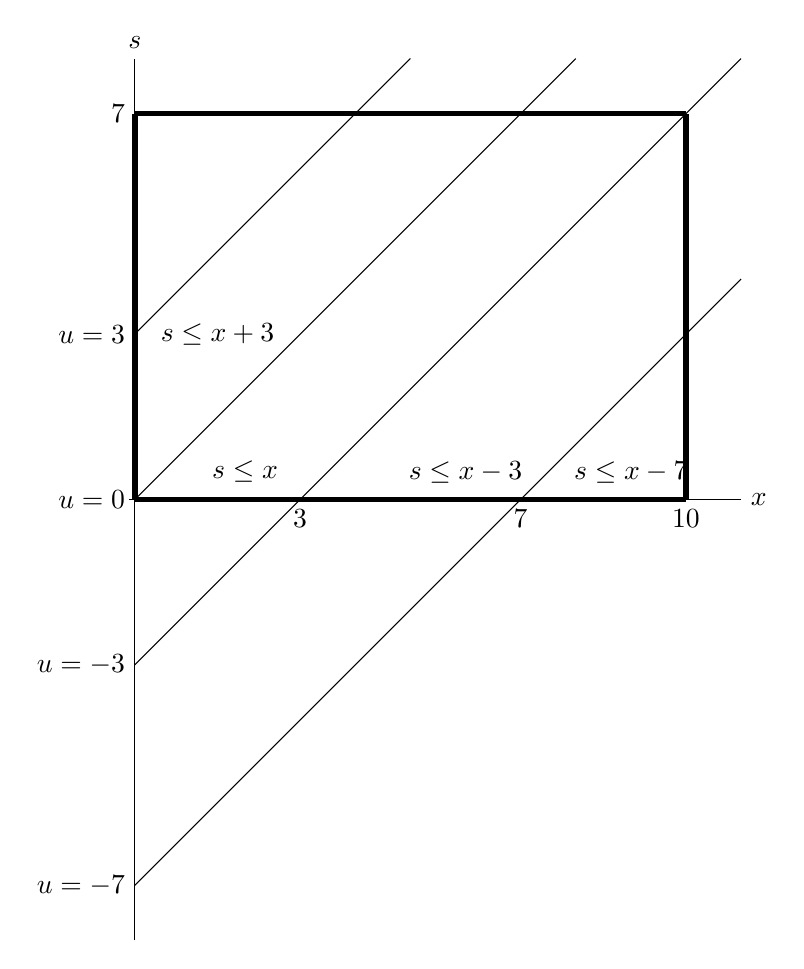
\begin{tikzpicture}[scale=0.7]
%\draw[[-{Triangle[open]},dotted] (0,10)--(8.5,10);
\draw (0,-8)--(0,8);
\node[right] at (11,0) {$x$};
\draw (-0.1,0)--(11,0);
\node[above] at (0,8) {$s$};
\draw[line width=0.7mm] (0,7)--(10,7);
\draw[line width=0.7mm] (10,0)--(10,7);
\draw[line width=0.7mm] (0,0)--(10,0);
\draw[line width=0.7mm] (0,0)--(0,7);
\node[below] at (10,0) {10};
\node[below] at (7,0) {7};
\node[below] at (3,0) {3};
\node[left] at (0,7) {7};
\draw (0,-7)--(11,4);
\node[left] at (0,-7) {$u=-7$};
\node at (9,0.5) {$s\leq x - 7$};
\draw (0,-3)--(11,8);
\node[left] at (0,-3) {$u=-3$};
\node at (6,0.5) {$s\leq x - 3$};
\draw (0,0)--(8,8);
\node[left] at (0,0) {$u=0$};
\node at (2,0.5) {$s\leq x$};
\draw (0,3)--(5,8);
\node[left] at (0,3) {$u=3$};
\node at (1.5,3) {$s\leq x+3$};
\end{tikzpicture}
\end{center}
%\caption{Computing the probability that $S-X\leq u$.}
%\label{fig:P_S_X}
%\end{figure}


It is clear that  the indicated rectangle has no overlap with the set of points $(x,s)$ such that $s\leq u + x$ for $u<-10$. (To see this, draw the line $s=x-10$ in the figure.) At $u=-10$, the overlap is a single point, at $(10,0)$. Thus, 
\begin{equation*}
\P{S-X \leq u}=0, \quad \text{for } u\leq -10.
\end{equation*}

When $u\in[-10, -3]$ we need to integrate over the triangle that results from cutting the line $s=x+u$ with the rectangle. The area is 
\begin{equation*}
70\, \P{S-X \leq u}= \frac{(10+u)^2}2, \quad \text{for } -10 \leq u\leq -3,
\end{equation*}
where we multiply with $70$ to get the normalization right. 

When $u\in[-3, 0]$, we integrate over a parallellogram with base $3+u$ and height $7$ plus the triangle below the line $s=x-3$. The area is 
\begin{equation*}
70\, \P{S-X \leq u}= (3+u)7 + \frac{(10-3)^2}2=7u + \frac{91}2, \quad \text{for } -3 \leq u\leq 0.
\end{equation*}

For $u\in[0, 7]$, we integrate over the trapezoid that results from intersecting the set $\{(x,s) : x \leq s \leq s + u\}$ and the rectangle plus the parallellogram plus the triangle below the line $s=x-3$. The area is 
\begin{equation*}
70\, \P{S-X \leq u}=  \frac{7^2}2 - \frac{(7-u)^2}{2} + 3\cdot 7 + \frac{49}2 = 7 u - \frac{u^2}2 + \frac{91}2, \quad \text{for } 0\leq u\leq 7.
\end{equation*}

Finally, for $u\geq 7$, the set $s\leq x+u$ covers the entire rectangle. Hence, 
\begin{equation*}
70\, \P{S-X \leq u}=  70, \quad \text{for } 7\leq u.
\end{equation*}

Given the amount of effort I had to put into getting this answer, I wanted to check it. So I went to  Wolframalpha (which is a great site for symbolic computations), and typed this: 
\begin{verbatim}
\int_{0}^{10} \int_0^7 Boole[s<= x + u]  ds dx,
\end{verbatim}
so, once you know \LaTeX\/ you can use Wolframalpha.  Wolframalpha turned it to 
\begin{verbatim}
Integrate[Boole[s <= u + x], {x, 0, 10}, {s, 0, 7}]
\end{verbatim}
If you fill this in at Wolframalpa, you'll get the results that we obtained above in seconds, rather than in one hour or so (depending on your proficiency with carrying out integrals).
\end{solution}
\end{exercise}



\begin{exercise}
  A machine serves two types of jobs. The processing time of jobs of
  type $i$, $i=1,2$, is exponentially distributed with parameter
  $\mu_i$. The type $T$ of job is random and independent of anything
  else, and such that $\P{T=1} = p = 1-q = 1-\P{T=2}$. (An example
  is a desk serving men and women, both requiring different average
  service times, and $p$ is the probability that the customer in
  service is a man.)  Show that  the expected processing time  and  variance are given by
\begin{align*}
  \E X &= p \E{X_1}  + q \E{X_2} \\
\V X &= p \V{X_1} + q \V{X_2} + pq(\E{X_1} - \E{X_2})^2.
  \end{align*}
Interestingly, we see that even if $\V{X_1} = \V{X_2} = 0$, $\V X > 0$
if $\E{X_1} \neq \E{X_2}$. Bear this in mind; we will use these ideas
later when we discuss the effects of failures on the variance of
service times of jobs.
\begin{hint}
    Let $X$ be the processing (or service) time at the server, and
    $X_i$ the service time of a type $i$ job. Then, 
    \begin{equation*}
      X = \1{T=1} X_1 + \1{T=2} X_2,
    \end{equation*}
    where $\1{}$ is the indicator function, that is, $\1{A}=1$ if the
    event $A$ is true, and $\1{A}=0$ if $A$ is not true.   
\end{hint}
  \begin{solution}
With the hint, 
\begin{align*}
  \E X 
&= \E{\1{T=1} X_1} + \E{\1{T=2} X_2} \\
&= \E{\1{T=1}} \E{ X_1} + \E{\1{T=2}} \E{X_2}, \text{ by the independence of $T$}, \\
&= \P{T=1} /\mu_1 + \P{T=2}/ \mu_2 \\
&= p /\mu_1 + q/ \mu_2 \\
&= p \E{X_1}  + q \E{X_2}.
\end{align*}
(The next derivation may seem a bit long, but the algebra is
standard. I include all steps so that you don't have to use pen and
paper yourself if you want to check the result.) Next, using that
\begin{equation*}
\1{T=1}\1{T=2} = 0 \text{ and } \1{T=1}^2 = \1{T=1},
\end{equation*}
we get
\begin{align*}
  \V X 
&= \E{X^2} - (\E X)^2 \\
&= \E{\left(\1{T=1} X_1 + \1{T=2} X_2\right)^2} - \left(\frac{p}{\mu_1}+\frac{q}{\mu_2}\right)^2 \\
&= \E{\1{T=1} X_1^2 + \1{T=2} X_2^2} - \left(\frac{p}{\mu_1}+\frac{q}{\mu_2}\right)^2 \\ 
&= p \E{X_1^2} + q \E{X_2^2} - \left(\frac{p}{\mu_1}+\frac{q}{\mu_2}\right)^2 \\ 
&= p \V{X_1} + p (\E{X_1})^2 + q \V{X_2} + q(\E{ X_2})^2 - \left(\frac{p}{\mu_1}+\frac{q}{\mu_2}\right)^2 \\ 
&= p \V{X_1} + \frac{p}{\mu_1^2} + q \V{X_2} + \frac{q}{\mu_2^2} - \left(\frac{p}{\mu_1}+\frac{q}{\mu_2}\right)^2 \\ 
&= p \V{X_1} + q \V{X_2}
+ \frac{p}{\mu_1^2} + \frac{q}{\mu_2^2}
- \frac{p^2}{\mu_1^2}-\frac{q^2}{\mu_2^2}  -\frac{2pq}{\mu_1\mu_2}\\ 
&= p \V{X_1} + q \V{X_2}
+ \frac{p(1-p)}{\mu_1^2} + \frac{q(1-q)}{\mu_2^2}
-\frac{2pq}{\mu_1\mu_2}\\ 
&= p \V{X_1} + q \V{X_2}
+ \frac{pq}{\mu_1^2} + \frac{qp}{\mu_2^2}
-\frac{2pq}{\mu_1\mu_2}\\ 
&= p \V{X_1} + q \V{X_2}
+ pq(\E{X_1} - \E{X_2})^2.
\end{align*}
\end{solution}
\end{exercise}


Let $B$ be a discrete random variable  such that $\P{B = k} = f(k)$, where $f(k)$ is a given set of
probabilities. We write
\begin{equation*}
  G(k) = \P{B>k} = \sum_{m=k+1}^\infty f(m),
\end{equation*}
for the \emph{survivor function} of $B$.  We can write this with an indicator function as
\begin{equation*}
  G(k) = \sum_{m=0}^\infty \1{m>k} f(m),
\end{equation*}
which makes the compution of certain expressions quite a bit easier. 

\begin{exercise}\label{ex:5}
  Express the probability mass  $f(k)$ and the survivor function $G(k)$ in terms of the distribution $F(k)$ of the batch size $B$. Which of the following is true:
  $G(k) = 1-F(k)$, $G(k) = 1-F(k-1)$, or $G(k) = 1-F(k+1)$?
  \begin{hint}
This exercise is just meant to become familiar with the notation.
  \end{hint}
  \begin{solution}
    \begin{align*}
    f(k) &= \P{B=k} = \P{B\leq k} - \P{B\leq k-1} = F(k)-F(k-1), \\
    G(k) &= \P{B>k} = 1 - \P{B\leq k} = 1-F(k).        
    \end{align*}
    It is all too easy to make, so called, off-by-one errors, such as
    in the three alternatives above.  I nearly always check simple
    cases to prevent such simple mistakes. I advise you to acquire the
    same habit.
  \end{solution}
\end{exercise}


\begin{exercise}\label{ex:6}
 Use indicator functions to prove that $ \sum_{k=0}^\infty G(k) = \E B$.
    \begin{hint}
Write 
$\sum_{k=0}^\infty G(k) = \sum_{k=0}^\infty \sum_{m=k+1}^\infty \P{B=m}$, reverse the summations. Then realize that $\sum_{k=0}^\infty \1{k<m} = m$. 
You should be aware that this sort of problem is just a regular probability
  theory problem, nothing fancy. We use/adapt the tools you learned in
  calculus to carry out 2D integrals (or in this case 2D summations.)
    \end{hint}
\begin{solution}
Observe first that $\sum_{k=0}^\infty \1{m>k} = m$, since $\1{m>k}=1$ if $k<m$ and $\1{m>k} = 0$ if $k\geq m$. With this, 
\begin{align*}
\sum_{k=0}^\infty G(k) 
&= \sum_{k=0}^\infty \P{B>k} 
= \sum_{k=0}^\infty \sum_{m=k+1}^\infty \P{B=m}  \\
& = \sum_{k=0}^\infty \sum_{m=0}^\infty 1\{m>k\} \P{B=m} 
= \sum_{m=0}^\infty \sum_{k=0}^\infty 1 \{m>k\} \P{B=m} \\
&= \sum_{m=0}^\infty m\P{B=k} = \E B.
\end{align*}
In case you are interested in mathematical justifications: the
interchange of the two summations is allowed because the summands are
all positive. (Interchanging the order of summations or integration is
not allways allowed because the results can be different when part of
the integrand is negative. Check Fubini's theorem for more on this if
you are interested.)
\end{solution}
\end{exercise}

\begin{exercise}\label{ex:66}
 Use indicator functions to prove that
$\sum_{i=0}^\infty i G(i) =  \E{B^2}/2 - \E{B}/2.$
    \begin{hint}
$\sum_{i=0}^\infty i G(i) = \sum_{n=0}^\infty \P{B=n} \sum_{i=0}^\infty i 1\{n\geq i+1\}$,
and reverse the summations.
    \end{hint}
\begin{solution}
\begin{align*}
\sum_{i=0}^\infty i G(i)
&= \sum_{i=0}^\infty i \sum_{n=i+1}^\infty \P{B=n} = \sum_{n=0}^\infty \P{B=n} \sum_{i=0}^\infty i 1\{n\geq i+1\} \\
&= \sum_{n=0}^\infty \P{B=n} \sum_{i=0}^{n-1}i  = \sum_{n=0}^\infty \P{B=n} \frac{(n-1)n}{2} \\
&= \sum_{n=0}^\infty  \frac{n^2}{2} \P{B=n} - \frac{\E B}{2}
= \frac{\E{B^2}}{2} - \frac{\E B}{2}.
\end{align*}
\end{solution}
\end{exercise}


Let $S$ be a continuous random variable with distribution function $F$.  We write 
\begin{equation*}
  \E{X} = \int_0^\infty x \d F(x)
\end{equation*}
for the expection of $X$. Here $\d F(x)$ acts as a shorthand for $f(x) \d x$ when $X$ has a density. \footnote{For the interested $\int x \d F(x)$ is a Lebesgue-Stieltjes integral with respect to the measure induced by the distribution function $F$.}

\begin{exercise}
 Use indicator functions to prove that 
$   \E S = \int_0^\infty x \d F  = \int_0^\infty G(y) \d y,$
where $G(x) = 1 - F(x)$. 
\begin{hint}
$\E S = \int_0^\infty x \d F  = \int_0^\infty \int_0^\infty 1_{y\leq x} \d y \d F(x)$.
\end{hint}
\begin{solution}
\begin{equation*}
  \begin{split}
    \E{S} &= \int_0^\infty x \d F  = \int_0^\infty \int_0^x \d y \d F(x) \\
    & = \int_0^\infty \int_0^\infty 1_{y\leq x} \d y \d F(x)   = \int_0^\infty \int_0^\infty 1_{y\leq x} \d F(x) \d y\\
    & = \int_0^\infty \int_y^\infty \d F(x) \d y = \int_0^\infty G(y) \d y
  \end{split}
\end{equation*}
\end{solution}
\end{exercise}

\begin{exercise}
 Use indicator functions to prove that for  a continuous random
    variable $S$ with distribution function $F$, 
$\E{S^2} = \int_0^\infty x^2 \d F  = 2 \int_0^\infty y G(y) \d y,$
where $G(x) = 1 - F(x)$. 
\begin{hint}
$\int_0^\infty y G(y) \d y = \int_0^\infty y \int_0^\infty 1\{y\leq x\}f(x)\, \d x \d y$.
\end{hint}
\begin{solution}
  \begin{align*}
\int_0^\infty y G(y) \d y 
&=  \int_0^\infty y \int_y^\infty f(x)\, \d x \d y =  \int_0^\infty y \int_0^\infty 1\{y\leq x\}f(x)\, \d x \d y\\
&=  \int_0^\infty f(x) \int_0^\infty y 1\{y \leq x\}\, \d y \d x
=  \int_0^\infty f(x) \int_0^x y\, \d y \d x\\
&=  \int_0^\infty f(x) \frac{x^2}2 \d x =\frac{\E{S^2}}2.
  \end{align*}
\end{solution}
\end{exercise}

\begin{exercise}
 Use integration by parts to show that for  a continuous random
    variable $S$ with distribution function $F$ and survivor function $G=1-F$, 
$\int_0^\infty y G(y) \d y = \E{S^2}/2.$
\begin{solution}
  \begin{equation}
      \int_0^\infty y G(y) \d y 
= \frac{y^2}2 G(y) \bigg|_0^\infty  - \int_0^\infty \frac{y^2}2 g(y)\d y = \int_0^\infty \frac{y^2}2 f(y)\d y = \frac{\E{S^2}}2,
  \end{equation}
  since $g(y) = G'(y) = - F'(y) = - f(y)$.
\end{solution}
\end{exercise}

\begin{exercise}
  Use that $\E S = \int_0^\infty x \d F = \int_0^\infty G(y) \d y$ to
  check that  $\E S = \mu^{-1}$ if $F(x) = 1 - e^{-\mu x}$.
\begin{solution}
If $F(x) = 1 - e^{-\mu x}$, we obtain that 
\begin{equation*}
  \E S = \int_0^\infty e^{-\mu x} \d x =
  \mu^{-1}\int_0^\infty e^{-x} \d x = \mu^{-1}.
\end{equation*}
\end{solution}
\end{exercise}


\begin{comment}
\begin{exercise}
  Assume that the time $X$ to fail of a machine is uniformly
  distributed on the interval $[0,10]$. If the machine fails at time
  $t$, the cost to repair it is $h(t)$. What is the expected repair
  cost? 
  \begin{solution}
    Write for $F(x) = \P{X\leq x}$ and $f(x) = \d F(x)/\d x$ for the
    density of $F$.
    \begin{equation*}
      \begin{split}
\E{h(X)}
&= \int_0^{10} \E{h(X) \given X = x} \P{X\in \d x} \\
&= \int_0^{10} \E{h(x) \given X = x} \d F(x) \\
&= \int_0^{10} \E{h(x) \given X = x} F(\d x) \\
&= \int_0^{10} \E{h(x) \given X = x} f(x) \d x \\
&= \int_0^{10} h(x)\frac{\d x}{10}.
      \end{split}
    \end{equation*}
    Here we introduce some notation that is commonly used in the
    probabity literature to indicate the same conceptual idea, i.e,
    $\P{X\in \d x} = \d F(x) = F(\d x) = f(x) \d x$, where the last
    equality follows from the fact that $F$ has a density $f$
    everywhere on $[0,10]$. 

    The concept of conditional expectation is of fundamental
    importance in probability theory. Any \emph{good} probability book
    defines this concept as a random variable measurable with respect
    to some $\sigma$-algebra. In this course we will not deal with
    this elegant idea, due to lack of time. 
  \end{solution}
\end{exercise}
\end{comment}


\Closesolutionfile{hint}
\Closesolutionfile{ans}

\opt{solutionfiles}{
\subsection*{Hints}
\input{hint}
\subsection*{Solutions}
\input{ans}
}

%\clearpage  


%%% Local Variables:
%%% mode: latex
%%% TeX-master: "../queueing_book"
%%% End:

%\section{Poisson Distribution}
\label{sec:poisson-distribution}

\subsection*{Theory and Exercises}


\Opensolutionfile{hint}
\Opensolutionfile{ans}

In this section we provide motivation for the use of the Poisson process as an arrival process of customers or jobs at a shop, service station, or machine, to receive service.  In the exercises we derive numerous  properties of  this exceedingly important distribution; in the rest of the book we will use these results time and again.

Consider a stream of customers that enter a shop over time. Let us write $N(s, t)$ for
the number of customers that entered during a time interval of $(s,t]$. Clearly, as we do not know in advance how many customers will enter, we model $N(s,t)$ as a random variable for all
times $s$ and $t$.

Our first assumption is that the rate at which customers enter does not
significantly change over time. Then it is reasonable to assume that
the expected number of arrivals is proportional to the  length of
the interval. Hence, it is reasonable to assume that there exists some
constant~$\lambda$ such that
\begin{equation}
  \label{eq:6}
 \E{N(s,t)} = \lambda (t-s).
\end{equation}
The constant $\lambda$ is often called the \recall{arrival rate}.


The second assumption is that $\{N(s,t), s\leq t\}$ has
\recall{stationary} and \emph{independent increments}. Stationarity
means that the distribution of the number of arrivals are the same for
all intervals of equal length. Formally, $N(s_1,t_1)$ has the same
distribution as $N(s_2, t_2)$ if $t_2-s_2 = t_1-s_1$. Independence
means, roughly speaking, that knowing that $N(s_1,t_1)= n$, does not
help to make any predictions about $N(s_2, t_2)$ if the intervals
$(s_1,t_1)$ and $(s_2, t_2)$ have no overlap.

To find the distribution of $N(t) = N(0,t)$, let us split the interval
$[0,t]$ into $n$ sub-intervals, all of equal length, and ask: `What is
the probability that a customer arrives in some given
sub-interval.'  By our second assumption, the arrival rate is
constant over time. Therefore, the probability $p$ of an arrival in each
interval should be constant. Moreover,
if the time intervals are very small, we can safely neglect the
probability that two or more customers arrive in one such tiny interval.

As a consequence, then, we can model the occurrence of an arrival in
some period $i$ as a Bernoulli distributed random variable $B_i$ such
that $p=\P{B_i =1}$ and $\P{B_i=0} = 1-\P{B_i = 1}$, and we assume that
$\{B_i\}$ are independent. The total number of failures $N_n(t)$ that
occur in $n$ intervals is then binomially distributed
\begin{equation}\label{eq:bin}
  \P{N_n(t) = k} = {n \choose k} p^k (1-p)^{n-k}.
\end{equation}

\begin{exercise}
Show that $\E{N_n(t)} = \sum_{i=1}^n \E{B_i} = n p$.
\begin{hint}
Use that $\E{X+Y} = \E X + \E Y$. 
\end{hint}
\begin{solution}
  \begin{equation*}
    \E{N_n(t)} = \E{\sum_{i=1}^n {B_i}} = \sum_{i=1}^n \E{B_i} = n \E{B_i} = n p.
  \end{equation*}
\end{solution}
\end{exercise}

\begin{exercise}
What is the difference between $N_n(t)$ and $N(t)$?
\begin{solution}
  $N_n(t)$ is a binomially distributed random variable with parameters
  $n$ and $p$. The maximum value of $N_n(t)$ is $n$. The random
  variable $N(t)$ models the number of failures that can occur during
  $[0,t]$. As such it is not necessarily bounded by $n$. Thus, $N_n(t)$ and $N(t)$ cannot represent the same random variable. 
\end{solution}
\end{exercise}


In fact, in some appropriate sense, $N_n(t)$ converges to $N(t)$ for $n\to \infty$ such
that
\begin{equation}\label{eq:pois}
  \P{N(t) = k} = 
e^{-\lambda t} \frac{(\lambda t)^k}{k!}.
\end{equation}
We say that $N(t)$ is \recall{Poisson distributed} with rate
$\lambda$, and write $N(t)\sim P(\lambda t)$. 

\begin{exercise}
  Show how the binomial distribution~\eqref{eq:bin} converges to the
  Poisson distribution~\eqref{eq:pois} if $n\to\infty$, $p\to0$ such
  that $np=\lambda$. 
  \begin{hint}
First find $p$, $n$, $\lambda$ and $t$ such that the rate
    at which event occur in both processes are the same. Then consider
    the binomial distribution and use the standard limit
    $(1-x/n)^n \to e^{-x}$ as $n\to \infty$. 
  \end{hint}
  \begin{solution} Now we like to relate $N_n(t)$ and $N(t)$. It is
    clear that we at least want the expectations to be the same, that
    is, $np = \lambda t$. This implies that
\begin{equation*}
  p = \frac{\lambda t}n.
\end{equation*}
Substituting this in this in the expression for $\P{N_n(t)=k}$ gives
\begin{equation*}
  \P{N_n(t) = k} = {n \choose k} \left(\frac{\lambda t}{n}\right)^k \left(1-\frac{\lambda t}n\right)^{n-k}.
\end{equation*}
To see that 
\begin{equation*}\label{eq:52}
  \lim_{n\to\infty} {n \choose k} \left(\frac{\lambda t}{n}\right)^k \left(1-\frac{\lambda t}n\right)^{n-k} = e^{-\lambda t} \frac{(\lambda t)^k}{k!}.
\end{equation*}
use that
    \begin{equation*}
      \begin{split}
      {n \choose k} \left(\frac{\lambda t}{n}\right)^k \left(1-\frac{\lambda t}n\right)^{n-k} 
&= \frac{n!}{k!(n-k)!} \left(\frac{\lambda t}{n}\frac{n}{n-\lambda t}\right)^k \left(1-\frac{\lambda t}n\right)^{n} \\
&= \frac{(\lambda t)^k}{k!} \left(\frac n{n-\lambda t} \right)^k  \frac{n!}{n^k(n-k)!}\left(1-\frac{\lambda t}n\right)^{n}\\
&= \frac{(\lambda t)^k}{k!} \left(\frac n{n-\lambda t} \right)^k \frac{n}{n}\frac{n-1}{n}\cdots\frac{n-k+1}{n} \left(1-\frac{\lambda t}n\right)^{n}.
\end{split}
\end{equation*}
Observe now that, as $\lambda t$ is finite, $n/(n-\lambda t)\to 1$ as
$n\to \infty$. Also for any finite $k$, $(n-k)/n\to1$. Finally, we use
that $(1+x/n)^n\to e^{x}$ so that ,
$\left(1-\frac{\lambda t}n\right)^{n} \to e^{-\lambda t}$.  The rest
is easy, so that, as $n\to\infty$,  the above converges to 
\begin{equation*}
\frac{(\lambda t)^k}{k!} e^{-\lambda t}.
\end{equation*}

  \end{solution}
\end{exercise}

Thus, if we assume that the arrival rate of customers is constant for some amount of time, e.g., an hour in a shop, and we assume that the probability of a customer arriving in some very small amount of time,  e.g., a milli second, is small, the resulting number arrival of customers is Poisson distributed. 


\begin{exercise}
  Show that if $N(t)\sim P(\lambda t)$, $\E{N(t)} = \lambda t$.
  \begin{solution} 
    When a random variable $N$ is Poisson distributed with parameter
    $\lambda$,
    \begin{equation*}
      \begin{split}
      \E N 
&= \sum_{n=0}^\infty n e^{-\lambda}\frac{\lambda^n}{n!}  \\
&= \sum_{n=1}^\infty n e^{-\lambda}\frac{\lambda^n}{n!}, \text{ since the term with $n=0$ cannot contribute} \\
&= e^{-\lambda} \lambda \sum_{n=1}^\infty \frac{\lambda^{n-1}}{(n-1)!} \\
&= e^{-\lambda} \lambda \sum_{n=0}^\infty \frac{\lambda^{n}}{n!}, \text{ by a change of variable}\\
&= e^{-\lambda} \lambda e^{\lambda} \\
&= \lambda.
      \end{split}
    \end{equation*}
\end{solution}
\end{exercise}


\begin{exercise}
  Show that if $N(t)\sim P(\lambda t)$, $\V{N(t)} = \lambda t$. 
  \begin{solution} 
Using that $\V N = \E{N^2} - (\E N)^2$, 
    \begin{equation*}
      \begin{split}
      \E{N^2}
&= \sum_{n=0}^\infty n^2 e^{-\lambda}\frac{\lambda^n}{n!}  \\
&= e^{-\lambda} \sum_{n=1}^\infty n \frac{\lambda^n}{(n-1)!}  \\
&= e^{-\lambda} \sum_{n=0}^\infty (n+1) \frac{\lambda^{n+1}}{n!}  \\
&= e^{-\lambda} \lambda \sum_{n=0}^\infty n \frac{\lambda^{n}}{n!}  +e^{-\lambda}\lambda \sum_{n=0}^\infty\frac{\lambda^{n}}{n!}  \\
&= \lambda^2  + \lambda.
\end{split}
\end{equation*}
\end{solution}
\end{exercise}

With moment generating functions we compute the mean and variance of $N(t)$ with less effort. 
Recall that the \recall{moment generating function}  of a random variable $X\geq 0$ and $t$ a real number is defined as
\begin{equation*}
  M_X(t) = \E{e^{tX}}.
\end{equation*}


\begin{exercise}
Show that the moment generating function of a Poisson distributed random variable $N(t)$ is
$M_{N(t)}(s)=  \E{e^{sN(t)}}  = \exp{\lambda t(e^s-1)}$.
  \begin{hint}
    Use that $\P{N(t)=k}=e^{-\lambda t}(\lambda t)^k/k!$
  \end{hint}
\begin{solution}
Since $N(t)$ is Poisson distributed with parameter $\lambda t$, 
\begin{equation*}
  \begin{split}
M(s)
&=  \E{e^{N(t)}} \\
&= \sum_{k=0}^\infty e^{s k} \P{N=k} \\
&= \sum_{k=0}^\infty e^{s k} \frac{(\lambda t)^k}{k!} e^{-\lambda t}  \\
&= e^{-\lambda t} \sum_{k=0}^\infty  \frac{(e^s \lambda t)^k}{k!}  \\
&= \exp(-\lambda t + e^s \lambda t) =\exp(\lambda t(e^s - 1)).
  \end{split}
\end{equation*}
\end{solution}
\end{exercise}

\begin{exercise}
Use  the moment generating function of $N(t)$ to compute $\E{N(t)}$ and $\V{N(t)}$. 
\begin{hint}
  Recall that $M'(0) = \E{N(t)}$ and $M''(s)= \E{(N(t))^2}$. 
\end{hint}
\begin{solution}
Using the expression for the moment generating function of the previous exercise,
  \begin{equation*}
    M'(s) = \lambda t e^s \exp(\lambda t(e^s - 1)).
  \end{equation*}
Hence $\E{N(t)} = M'(0) = \lambda t $. Next, 
  \begin{equation*}
    M''(s) = (\lambda t e^s + (\lambda t e^s)^2) \exp(\lambda t(e^s - 1)),
  \end{equation*}
hence $\E{(N(t))^2} = M''(0) = \lambda t + (\lambda t)^2$. And thus, 
\begin{equation*}
\V{N(t)} =\E{(N(t))^2}-(\E{N(t)})^2 = \lambda t + (\lambda t)^2 - (\lambda t)^2 = \lambda t.
\end{equation*}
\end{solution}
\end{exercise}

Define the \emph{square coefficient  of variation (SCV)} of a random variable~$X$ as 
\begin{equation*}
  C^2= \frac{\V X}{(\E X)^2}.
\end{equation*}
As  will become clear later, the SCV is a very important concept in
  queueing theory. Memorize it as a measure of \emph{relative
  variability}.

\begin{exercise}
Show that   the SCV of $N(t)$ is equal to $1/\lambda t$. 
  \begin{solution}
    \begin{equation*}
SCV = \frac{\V{N(t)}}{(\E{N(t)})^2} = \frac{\lambda t}{(\lambda t)^2} = \frac1{\lambda t}.
    \end{equation*}

  \end{solution}
\end{exercise}

For the next couple of exercises, we need the concept of conditional probability. To help you recall this, consider the next question.

\begin{exercise} 
  We have to give one present to one of three children. As we cannot
  divide the present into parts, we decide to let `fate decide'. That
  is, we choose a random number in the set $\{1, 2, 3\}$. The first
  child that guesses the number wins the present. Show that the
  probability of winning the present is the same for each child.
  \begin{hint}
    For the second child, condition on the event that the first does not chose the right number.
    Use the definition of conditional probability:
    \begin{equation*}
    \P{A|B} = \frac{\P{AB}}{\P{B}}, 
    \end{equation*}
provided $\P{B}>0$.
  \end{hint}
\begin{solution}
    The probability that the first child to guess also wins is
    $1/3$. What is the probability for child number two? Well, for
    him/her to win, it is necessary that child one does not win and
    that child two guesses the right number of the remaining
    numbers. Assume, without loss of generality that child 1 chooses
    $3$ and that this is not the right number. Then 
    \begin{equation*}
      \begin{split}
&\P{\text{Child  2 wins}} \\
&= \P{\text{Child 2 guesses the right number and child 1 does not win}} \\
&= \P{\text{Child 2 guesses the right number} \given \text{ child 1 does not win}}
\cdot \P{\text{Child 1 does not win}} \\
&= \P{\text{Child 2 makes the right guess in the set $\{1,2\}$}}\cdot \frac 23 \\
&= \frac 1 2\cdot \frac 23  = \frac 1 3.
      \end{split}
    \end{equation*}
    Similar conditional reasoning gives that child 3 wins with probability $1/3$. 
  \end{solution}
\end{exercise}



\begin{exercise}
  Show that if $N(t) \sim P(\lambda t)$, we have for small $h$,
$\P{N(h) = n \given N(0) = n} = 1-\lambda h + o(h)$.
\recall{Recall} that  $o(h)$ is a function  $f(h)$ such $f(h)/h \to 0$ as $h\to 0$.
    \begin{hint}
Recall the definition of the conditional probability $\P{A\given B} = \P{AB}/\P{B}$, where we write $AB = A\cap B$. This definition only holds when $\P{B} > 0$. 

    Think about the meaning of the formula
      $\P{N(h) = n \given N(0) = n}$. It is a conditional probability
      that should be read like this: given that up to time $0$ we have
      seen $n$ arrivals (i.e, $N(0)=n$), what is the probability that
      just a little later ($h$) the number of arrivals is still $n$,
      i.e, $N(h)=n$? Then use the definition of the Poisson
      distribution to compute this probability. Finally, use Taylor's
      expansion of $e^{x}$ to see that $e^{x} = 1 +x + o(x)$ for
      $|x| \ll 1$.  
    \end{hint}
\begin{solution}
    \begin{equation*}
      \begin{split}
  \P{N(h) = n | N(0) = n} 
&=  \P{N(h) = n \& N(0) = n}/\P{N(0)=n} \\
&=  \P{N(h) = n} \P{N(0) = n}/\P{N(0)=n}, \\
& \quad\text{(by independence of } N(h)=n\text{ and } N(0)=n)\\
&= \P{N(h) = 0} \\
&= e^{-\lambda h} (\lambda h)^0/0! \\
&= e^{-\lambda h} = 1-\lambda h + o(h),
      \end{split}
    \end{equation*}
  as follows from a standard argument in analysis that
  $e^{-\lambda h} = 1 -\lambda h + o(h)$  for $h$ small. 
\end{solution}
\end{exercise}

\begin{exercise}
  Show that if $N(t) \sim P(\lambda t)$, we have for small $h$,
 $\P{N(h) = n+1 \given N(0) = n} = \lambda h + o(h)$. 
    \begin{hint} Use the previous exercise.
    \end{hint}
\begin{solution}
  \begin{equation*}
    \begin{split}
  \P{N(h) = n +1 | N(0) = n} 
&= \P{N(h) = 1} = e^{-\lambda h} (\lambda h)^1/1! \\
&= (1-\lambda h + o(h))\lambda h  = \lambda h - \lambda^2 h^2 + o(h) \\
&= \lambda h + o(h). 
    \end{split}
  \end{equation*}
\end{solution}
\end{exercise}

\begin{exercise}
  Show that if $N(t) \sim P(\lambda t)$, we have for small $h$,
 $\P{N(h) \geq n+2 \given N(0) = n} = o(h)$.
    \begin{hint}
 Use that  $\sum_{i=2}^\infty x^i/i! = \sum_{i=0}^\infty x^i/i! - x -1 = e^x -x - 1$.
    \end{hint}
\begin{solution}
  \begin{equation*}
    \begin{split}
  \P{N(h) \geq n+2 | N(0) = n} 
&= \P{N(h) \geq 2} \\
&= e^{-\lambda h} \sum_{i=2}^\infty \frac{(\lambda h)^i}{i!} 
= e^{-\lambda h} \left(\sum_{i=0}^\infty \frac{(\lambda h)^i}{i!} - \lambda h - 1\right)\\
&= e^{-\lambda h}(e^{\lambda h} - 1 - \lambda h) 
= 1 - e^{-\lambda h}(1 + \lambda h) \\
&= 1 - (1-\lambda h + o(h))(1+\lambda h) 
= 1 - (1-\lambda^2 h^2 + o(h)) \\
&= \lambda^2 h^2 + o(h) = o(h).
    \end{split}
  \end{equation*}

We can also use the results of the previous parts to see that
\begin{equation*}
    \begin{split}
  \P{N(h) \geq n+2 | N(0) = n} 
&= \P{N(h) \geq 2} = 1- \P{N(h)<2} \\
&= 1 - \P{N(h)= 0} - \P{N(h)=1} \\
&= 1 - (1-\lambda h) + o(h) ) - (\lambda h + o(h)) \\
&= o(h).
\end{split}  
\end{equation*}
\end{solution}
\end{exercise}

We define the Poisson \emph{process} as the set $N=\{N(t), t\geq 0\}$. Observe that this process is a much more complicated object than the Poisson distributed random variable $N(t)$. The
process is an uncountable set of random variables $N(t)$ for all $t\geq 0$, whereas $N(t)$ is just \emph{one} random variable.

\begin{exercise}
Show that  for a Poisson process $N$, 
$ \P{N(0,s] =1\given N(0,t]=1} = s/t$. Thus, if you know that $N(0,t]=1$, the arrival is distributed
uniformly on the interval $[0,t]$.
\begin{hint}
 Observe that 
  \begin{equation*}
\{N(0,s]+N(s,t]=1\}\cap\{N(0,s]=1\} = \{1+N(s,t]=1\}\cap\{N(0,s]=1\}=\{N(s,t]=0\}\cap\{N(0,s]=1\};
  \end{equation*}
these two events are independent.
\end{hint}
\begin{solution}
\begin{equation*}
  \begin{split}
  \P{N(0,s] =1\given N(0,t]=1} 
&= \frac{\P{N(0,s] =1, N(0,t]=1}}{\P{N(0,t]=1}} \\
&=   \P{N(0,t] =1\given N(0,s]=1} \frac{\P{N(0,s] =1}}{\P{N(0,t]=1}} \\
&=   \P{N(0,s] + N(s,t] =1\given N(0,s]=1} \frac{e^{-\lambda s}\lambda s}{e^{-\lambda t} \lambda t} \\
&=   \P{1 + N(s,t] =1\given N(0,s]=1} e^{-\lambda (s-t)} \frac{s}{t} \\
&=   \P{N(s,t] =0} e^{-\lambda (s-t)} \frac{s}{t} = e^{-\lambda(t-s)} e^{-\lambda (s-t)} \frac{s}{t} = \frac st.
  \end{split}
\end{equation*}
\end{solution}
\end{exercise}

\emph{Merging}, or the \emph{superposition}, of Poisson processes occurs often in practice.  We have two Poisson processes, for instance, the arrival processes $N_\lambda$ of men
and $N_\mu$ women at a shop. In the figure below, each cross represents an arrival, in the upper line it corresponds to a man, in the middle to a woman, in lower line to an
arrival of a general customer at the shop. Thus,  the shop `sees' the superposition $N_{\lambda+\mu}$ of these two arrival processes. 

  \begin{center}
\begin{tikzpicture}[scale=1]
%\draw[[-{Triangle[open]},dotted] (0,10)--(8.5,10);

\draw[->] (0,2)--(10,2);
\node[left] at (0,2) {$N_\lambda(t)$};
\draw[->] (0,1)--(10,1);
\node[left] at (0,1) {$N_\mu(t)$};
\draw[->] (0,0)--(10,0);
\node[left] at (0,0) {$N_{\lambda+\mu}(t)$};

\draw[{Rays[]}-{Rays[]},dotted] (1,2.06)--(1,-0.06);
\draw[{Rays[]}-{Rays[]},dotted] (1.5,1.06)--(1.5,-0.06);
\draw[{Rays[]}-{Rays[]},dotted] (3.2,2.06)--(3.2,-0.06);
\draw[{Rays[]}-{Rays[]},dotted] (3.5,1.06)--(3.5,-0.06);
\draw[{Rays[]}-{Rays[]},dotted] (4.5,1.06)--(4.5,-0.06);
\draw[{Rays[]}-{Rays[]},dotted] (5,1.06)--(5,-0.06);
\draw[{Rays[]}-{Rays[]},dotted] (6.1,1.06)--(6.1,-0.06);
\draw[{Rays[]}-{Rays[]},dotted] (7.1,2.06)--(7.1,-0.06);
\end{tikzpicture}
\end{center}

For the next set of exercises,  assume that $N_\lambda(t)\sim \text{P}(\lambda t)$, $N_\mu(t) \sim \text{P}(\mu t)$ and are independent.

\begin{exercise} 
Show that   $N_{\lambda+\mu}(t)=N_\lambda(t) + N_\mu(t) \sim \text{P}((\lambda + \mu)t)$. Thus, when we merge two independent Poisson processes, the merged process is also a Poisson process whose rate is the sum of the rates of the original Poisson processes.
  \begin{hint}
Use a conditioning argument or use moment generating functions.

In particular, for
    conditioning, use that $\P{AB} = \P{A\given B}\P{B}$. More
    generally, if the set $A$ can be split into disjoint sets $B_i$,
    i.e, $A=\bigcup_{i=1}^n B_i$, then
    \begin{equation*}
      \P{A} = \sum_{i=1}^n \P{A B_i} = \sum_{i=1}^n \P{A\given B_i} \P{B_i},
    \end{equation*}
    where we use the conditioning formula to see that
    $\P{A B_i} = \P{A \given B_i} \P{B_i}$.  Now choose practical sets
    $B_i$.  
  \end{hint}
    \begin{solution}
First we show how to  use conditioning. 
  \begin{equation*}
    \begin{split}
\P{N_\lambda(t) + N_\mu(t) = n} 
&= \sum_{i=0}^n \P{N_\lambda(t) + N_\mu(t) = n|N_\lambda(t) = i}\P{N_\lambda(t)=i} \\
\end{split}
\end{equation*}
Now, if $N_\lambda(t)=i$, then 
\begin{equation*}
N_\lambda(t)+N_\mu(t) = n \iff 
i+N_\mu(t) = n \iff 
N_\mu(t) = n-i.
\end{equation*}
Thus,
  \begin{equation}\label{eq:002}
    \begin{split}
\P{N_\lambda(t) + N_\mu(t) = n} 
&= \sum_{i=0}^n \P{ N_\mu(t) = n-i}\P{N_\lambda(t)=i} \\
&= \sum_{i=0}^n \frac{(\mu t)^{n-i}}{(n-i)!} \frac{(\lambda t)^i}{i!} e^{-(\mu+\lambda)t} \\
&= e^{-(\mu+\lambda)t} \sum_{i=0}^n \frac{(\mu t)^{n-i}}{(n-i)!} \frac{(\lambda t)^i}{i!}  \\
&= e^{-(\mu+\lambda)t}\frac 1{n!} \sum_{i=0}^n {n \choose i }(\mu t)^{n-i}(\lambda t)^i  \\
&= \frac{((\mu+\lambda)t))^n}{n!}e^{-(\mu+\lambda)t}.
    \end{split}
  \end{equation}

Now with the moment generating functions of $N_\lambda(t)$ and $N_\mu(t)$, and using that by the independence of  $N_\lambda(t)$ and $N_\mu(t)$, the moment generating function of $N_\lambda + N_\mu$ is the product of the moment generating functions of $N_\lambda$ and $N_\mu$, 
\begin{equation*}
  \begin{split}
M_{N_\lambda(t)+N_\mu(t)}(s) 
&= M_{N_\lambda(t)}(s) M_{N_\mu(s)} \\
&=\exp(\lambda t (e^s -1)) \exp(\mu t(e^s-1)) \\
&= \exp((\lambda + \mu)t (e^s-1)).
  \end{split}
\end{equation*}
Finally, since  generating function uniquely characterizes
the distribution, and since the above expression has the same form as a Poisson random variable  with parameter $(\lambda+\mu)t$, we can conclude that $N(t)\sim P((\lambda +\mu) t)$.
    \end{solution}
\end{exercise}


\begin{exercise}
What is the
  meaning of the event
  $\{N_\lambda(h) = 1, N_\mu(h) = 0\}\cap\{N_\lambda(h) + N_\mu(h) = 1\}$?
    \begin{solution}
 This means that, given that an event occurred, the event was an arrival, i.e., $N_\lambda$ was the first.
    \end{solution}
\end{exercise}

\begin{exercise} 
Use that  $N_\lambda(t) + N_\mu(t) \sim \text{P}((\lambda + \mu)t)$ to conclude
    \begin{equation*}
    \P{N_\lambda(h) = 1,  N_\mu(h) = 0 | N_\lambda(h) + N_\mu(h) = 1} =
\frac{\lambda}{\lambda+\mu}.
    \end{equation*}
    Note that the right-hand-side does not depend on $h$, hence it
    holds for any time $h$, whether it is small or not.  
    \begin{hint}
Suppose
      we write $N(t)=N_\lambda(t) + N_\mu(t)$. Then
      \begin{equation*}
      \P{N_\lambda(h) = 1, N_\mu(h) = 0 | N(h) = 1}
      \end{equation*}
      is the probability that $N_\lambda(h)=1$ and $N_\mu(h)=0$ \emph{given}
      that $N(t)=1$. In other words, the question is find out that,
      given one of the two processes `fired', what is the probability
      that $N_\lambda$ was the one that `fired'.
    \end{hint}
    \begin{solution}
  With the above:
  \begin{equation*}
    \begin{split}
&    \P{N_\lambda(h) = 1,  N_\mu(h) = 0 | N_\lambda(h) + N_\mu(h) = 1} \\
&= \frac{\P{N_\lambda(h) = 1,  N_\mu(h) = 0, N_\lambda(h) + N_\mu(h) = 1} }{ \P{N_\lambda(h) + N_\mu(h) = 1}} \\ 
&= \frac{\P{N_\lambda(h) = 1,  N_\mu(h) = 0}}{ \P{N_\lambda(h) + N_\mu(h) = 1}} \\ 
&= \frac{\P{N_\lambda(h) = 1}\P{N_\mu(h) = 0}}{ \P{N_\lambda(h) + N_\mu(h) = 1}} \\ 
&= \frac{\lambda h \exp(-\lambda h) \exp(-\mu h)}{((\lambda+\mu)h)\exp{(-(\lambda+\mu)h)}}\\
&= \frac{\lambda h \exp{(-(\lambda + \mu)h)}}{((\lambda+\mu)h)\exp{(-(\lambda+\mu)h)}}\\
&= \frac{\lambda}{\lambda+\mu}.
    \end{split}
  \end{equation*}
    \end{solution}
\end{exercise}


Besides merging Poisson streams, we can also consider the concept of \emph{splitting}, or \emph{thinning}, a stream into substreams, as follows.  When a customer arrives, throw a coin that lands   heads with probability $p$ and tails with $q=1-p$. When the coin   lands heads, the customer is of type 1 (e.g., a woman), otherwise of type 2 (e.g., a child).  Another   way of thinning is by modeling the stream of people passing a shop   as a Poisson process with rate $\lambda$. With probability $p$ a   person decides, independent of anything else, to enter the shop,  c.f. the figure below. The crosses at the upper line are passersby  in the street. The crosses at the lower line are the customers that   enter the shop. The outcome of the $k$th throw of a coin is   indicated by $B_k$. In the figure below,  $B_1=1$ so that the first passerby turns into a
  customer entering the shop; the second passerby does not enter as   $B_2=0$, and so on. Like this, the stream of passerby's is thinned   with Bernoulli distributed random variables.

  \begin{center}
\begin{tikzpicture}[scale=1]
%\draw[[-{Triangle[open]},dotted] (0,10)--(8.5,10);
\draw[->] (0,2)--(10,2);
\node[left] at (0,2) {$N_\lambda(t)$};
%\draw[->] (0,1)--(10,1);
%\node[left] at (0,1) {$B_k$};
\draw[->] (0,0)--(10,0);
\node[left] at (0,0) {$N_{\lambda p}(t)$};

\draw[{Rays[]}-{Rays[]},dotted] (1,2.06)--(1,-0.06) 
node[below]  {$B_1=1$};

\draw[{Rays[]}-{Circle[open]},dotted] (2.5,2.06)--(2.5,1.3) 
node[below] {$B_2=0$};

\draw[{Rays[]}-{Circle[open]},dotted] (4,2.06)--(4,1.3) 
node[below, fill=white] {$B_3=0$};

\draw[{Rays[]}-{Rays[]},dotted] (5,2.06)--(5,-0.06) 
node[below]  {$B_4=1$};

\draw[{Rays[]}-{Rays[]},dotted] (6.5,2.06)--(6.5,-0.06) 
node[below]  {$B_5=1$};


\draw[{Rays[]}-{Circle[open]},dotted] (7.5,2.06)--(7.5,1.3) 
node[below, fill=white] {$B_6=0$};

\end{tikzpicture}
  \end{center}

 
The concept of merging and thinning are also  useful to analyze queueing
  networks. Suppose the departure stream of a machine splits into
  two substreams, e.g., a fraction $p$ of the jobs moves to on another
  machine and the rest ($1-p$) of the jobs leaves the system. Then we
  can model the arrival stream at the second machine as a thinned
  stream (with probability $p$) of the departures of the first
  machine. Merging occurs where the output streams of various stations arrive at another station.

\begin{exercise}
Show that the Poisson process obtained by thinning the original
  process is $\sim P(\lambda t p)$ for any~$t$.
  \begin{hint}
 Condition on the total number of arrivals $N(t)=m$ up to time
      $t$. Realize that the probability that a job is of type 1 is
      Bernoulli distributed, hence when you consider $m$ jobs in
      total, the number of type 1 jobs is binomially distributed.

      Again use that if the set $A$ can be split into disjoint sets
      $B_i$, i.e, $A=\bigcup_{i=1}^n B_i$, then
    \begin{equation*}
      \P{A} = \sum_{i=1}^n \P{A\given B_i} \P{B_i}.
    \end{equation*}
Now choose practical sets $B_i$. 


You might also consider the random variable 
  \begin{equation*}
    Y = \sum_{i=1}^N Z_i,
  \end{equation*}
  with $N\sim P(\lambda)$ and $Z_i\sim B(p)$. Show that the moment
  generating function of $Y$ is equal to the moment generating
  function of a Poisson random variable with parameter $\lambda p$.
  \end{hint}
    \begin{solution}
Suppose that  $N_1$ is the  thinned stream, and $N$ the total stream. Then
\begin{equation*}
  \begin{split}
    \P{N_1 = k}
&= \sum_{n=k}^\infty \P{N_1 =k, N = n} 
= \sum_{n=k}^\infty \P{N_1 =k\given N = n}\P{N=n} \\
&= \sum_{n=k}^\infty \P{N_1 =k\given N = n}e^{-\lambda} \frac{\lambda^n}{n!}
= \sum_{n=k}^\infty {n \choose k} p^k (1-p)^{n-k} e^{-\lambda} \frac{\lambda^n}{n!}\\
&= e^{-\lambda}\sum_{n=k}^\infty  \frac{p^k (1-p)^{n-k}}{k! (n-k)!} \lambda^n
= e^{-\lambda} \frac{(\lambda p)^k}{k!} \sum_{n=k}^\infty  \frac{(\lambda (1-p))^{n-k}}{(n-k)!}\\
&= e^{-\lambda} \frac{(\lambda p)^k}{k!} \sum_{n=0}^\infty  \frac{(\lambda (1-p))^{n}}{n!}
= e^{-\lambda} \frac{(\lambda p)^k}{k!} e^{\lambda(1-p)} \\
&= e^{-\lambda p} \frac{(\lambda p)^k}{k!}.
  \end{split}
\end{equation*}
We see that the thinned stream is Poisson with parameter $\lambda p$. (For notational ease, we left out the $t$, otherwise it is $P(\lambda t p)$. 

Now consider $Y=\sum_{i=1}^N Z_i$. Suppose that $N=n$, so that $n$
arrivals occurred. Then we throw $n$ coins with success probability
$p$. It follows that $Y$ is indeed a thinned Poisson random variable.
Model the coins as a generic Bernoulli distributed random variable
$Z$.  We first need
\begin{equation*}
  \E{e^{s Z}} = e^0 \P{Z=0} + e^{s} \P{Z=1} = (1-p) + e^s p.
\end{equation*}
Suppose that $N=n$, then since the $Z_i$ are i.i.d.,
\begin{equation*}
\E{e^{s\sum_{i=1}^n Z_i}} = \left(\E{e^{s Z}}\right)^n = \left(1 + p (e^s - 1)\right)^n
\end{equation*}
Then, using conditioning on $N$, 
\begin{equation*}
  \begin{split}
  \E{e^{s Y}}
&= \E{\E{e^{s\sum_{i=1}^n Z_i} \given N=n }} 
 = \E{\E{\left(1+p(e^s-1)\right)^n \given N=n }} \\
&= \sum_{n=0}^\infty \left(1+p(e^s-1)\right)^n e^{-\lambda} \frac{\lambda^n}{n!}
= e^{-\lambda} \sum_{n=0}^\infty \frac{\left(1+p(e^s-1)\right)^n \lambda^n}{n!}\\
&= \exp(-\lambda+ \lambda (1+p(e^s-1))) = \exp(\lambda p (e^s - 1)).
  \end{split}
\end{equation*}
Thus, $Y$ has the same moment generating function as a Poisson
distributed random variable with parameter $\lambda p$. Since
moment-generating functions specify the distribution uniquely,
$Y\sim P(\lambda p)$.
\end{solution}
\end{exercise}    

In fact, it can be proven that Poisson processes are the only arrival processes are such that, when merged  or thinned, the resulting processes are again Poisson processes. Thus, if you believe that it is reasonable that a thinned  processes has similar statistical properties as the original process, except that the mean becomes smaller, than the Poisson process is the only process that can be consistent with your intuition.


\Closesolutionfile{hint}
\Closesolutionfile{ans}
\subsection*{Hints}
\input{hint}
\subsection*{Solutions}
\input{ans}
\clearpage

%%% Local Variables:
%%% mode: latex
%%% TeX-master: "booktest"
%%% End:

% 
\section{Kendall's Notation to Characterize Queueing Processes}
\label{sec:kendalls-notation}



\Opensolutionfile{hint}
\Opensolutionfile{ans}

\subsection*{Theory and Exercises}

As will become apparent in Sections~\ref{sec:constr-discr-time}
and~\ref{sec:constr-gg1-queu}, the construction of any single-station queueing
process involves three main elements: 
the distribution of the
interarrival times between consecutive jobs, the distribution of the
service times of the individual jobs, and the number of servers
present to process jobs. In this characterization it is implicit that
the interarrival times form a set of i.i.d. (independent and
identically distributed) random variables, the service times are also
i.i.d., and finally, the interarrival times and service times are
mutually independent.

To characterize the type of queueing process it is common to use 
\recall{Kendall's} abbreviation $A/B/c/K$, where $A$ is the distribution of the
interarrival times, $B$ the distribution of the service times, $c$ the
number of servers, and $K$ system size, i.e., the total number of customers that can be simultaneously present, whether in queue or in service. In this notation it
is assumed that jobs are served in first-in-first-out (FIFO) order;
FIFO scheduling is also often called first-come-first-serve (FCFS). To specify the distributions $A$ and $B$ often two letters are used: $M$ to denote the exponential distribution as is is Memoryless, and $G$ to denote any General distribution. 

In the sequel we will often use Kendall's notation  to distinguish between the different queueing models. Ensure that you familiarize yourself with this notation. Let us therefore illustrate this notation with some exercises. 

\begin{exercise}
  What is the meaning of $M/M/1$?
  \begin{solution}
$M/M/1$: the distribution of the interarrival times is
  \emph{M}emory-less, hence exponential, the service times are also
  \emph{M}emoryless, and there is 1 server. As $K$ is unspecified, the system can contain any number of jobs.
  \end{solution}
\end{exercise}

\begin{exercise}
  By how many parameters is the $M/M/1$ queue characterized?
  \begin{solution}
    The interarrival times are exponentially distributed with rate $\lambda$; the service times are also exponential, but with parameter $\mu$. Thus, if we know $\lambda$ and $\mu$, we have fully characterized the parameters of both distributions. Since the number of servers is 1, only $\lambda$ and $\mu$ remain.
  \end{solution}
\end{exercise}

\begin{exercise}
What is the $D/D/1$ queue?  
\begin{solution}
  A queueing process with deterministic interarrival times and deterministic service times and 1 server.
\end{solution}
\end{exercise}

\begin{exercise}
  What is the meaning of $M/M/c$?
  \begin{solution}
$M/M/c$: A \recall{multi-server} queue with $c$ servers in which
  all servers have the same service capacity. Jobs arrive according to a
  Poisson process and have exponentially distributed processing times.
  \end{solution}
\end{exercise}

\begin{exercise}
  What is the meaning of $M/M/c/K$?
  \begin{solution}
\item $M/M/c/K$: interarrival times and process times are exponential,
  and the \recall{system capacity} is $K$ jobs. Thus, the queue can
  contain at most $K-c$ jobs. 

Note, sometimes, the $K$ stands for
    the capacity in the queue, not the entire system. The notation differs among
    authors.
  \end{solution}
\end{exercise}


\begin{exercise}
  What is the meaning of $M/M/c/c$?
  \begin{solution}
 In this system the number of servers is the same as
  the system capacity, thus the queue length is always zero. This
  queueing system is useful to determine the number of beds
  in a hospital; the beds act as servers.
  \end{solution}
\end{exercise}

\begin{exercise}
  What is the meaning of $M(n)/M(n)/1$?
  \begin{solution}
$M(n)/M(n)/1$: the interarrival times are exponential, just as
  the service times, but the rates of the arrival and service processes
  may depend on the queue length $n$. 
  \end{solution}
\end{exercise}


\begin{exercise}
  What is the meaning of $M^X/M/1$?
  \begin{solution}
 $M^X/M/1$: Customers arrive with exponentially distributed
  interarrival times. However, each customer brings in a number of
  jobs, known as a batch. The number of jobs in each batch is
  distributed as the random variable $X$. Thus, the arrival process of
  work is \recall{compound Poisson}.
  \end{solution}
\end{exercise}

\begin{exercise}
  What is the meaning of $M/G/1$?
  \begin{solution}
$M/G/1$: the interarrival times are exponentially distributed,
  the service times can have any \emph{G}eneral distribution (with
  finite mean), and there is 1 server.
  \end{solution}
\end{exercise}


\begin{exercise}
  What is the meaning of $M/G/\infty$?
  \begin{solution}
 $M/G/\infty$: exponential interarrival times, service times can
  have any distribution, and there is an unlimited supply of
  servers. This is also known as an \recall{ample} server. Observe
  that in this queueing process, jobs actually never have to wait in
  queue; upon arrival there is always a free server available.
  \end{solution}
\end{exercise}

\begin{exercise}
  What is the meaning of $G/G/1$?
  \begin{solution}
 $G/G/1$: generally distributed interarrival and service times, 1 server.
  \end{solution}
\end{exercise}

\begin{exercise}
  What is the meaning of $M/D/1-LIFO$?
  \begin{solution}
 $M/D/1-LIFO$.  Now job service times are \emph{D}eterministic, and the service sequence is last-in-first-out (LIFO).
  \end{solution}
\end{exercise}

\begin{exercise}
  Is the $M/D/1$ queue a specific type of  $M/G/c$ queue? 
  \begin{solution}
    Yes, take $G=D$ and $c=1$. 
  \end{solution}
\end{exercise}

\begin{exercise}
  What are some advantages and disadvantages of using the Shortest
  Processing Time First (SPTF) rule to serve jobs? 
  \begin{hint}
Look up the relevant
  definitions on wikipedia or
  \citet{hall91:_queuein_method_servic_manuf}
  \end{hint}
  \begin{solution}
  \begin{itemize}
  \item Advantage: SPTF minimizes the number of jobs in queue. Thus,
    if you want to keep the shop floor free of jobs (Work In Progress,
    WIP), then this is certainly a good rule. 
  \item Disadvantage: large jobs get near to terrible waiting times,
    and the variance of the waiting time increases. Thus, the $C_s^2$
    is larger than under FIFO. Also, SPTF does not take duedates into
    account, thus giving a reliable duedate quotation to a customer is
    hard (near to impossible.)
  \end{itemize}
  \end{solution}
\end{exercise}


\Closesolutionfile{hint}
\Closesolutionfile{ans}
\subsection*{Hints}
\input{hint}
\subsection*{Solutions}
\input{ans}
\clearpage

%%% Local Variables:
%%% mode: latex
%%% TeX-master: "book"
%%% End:

%%\section{Construction of Discrete-Time  Queueing Processes}
\section{Construction of Discrete-Time Queueing
  Processes}
\label{sec:constr-discr-time}

\subsection*{Theory and Exercises}

\Opensolutionfile{hint}
\Opensolutionfile{ans}


To provide real-life motivation to analyze queueing systems we discuss a case.  As this case is too hard to analyze by mathematical means,  we need to develop a model to simulate the queueing system in discrete time.  Interestingly, the structure of the simulation is very simple so that  it is also  an exceedingly convincing tool to communicate the results of an analysis of a queueing system to managers (and the like).  

Let us start with discussing the essentials of the simulation of a queueing system. The easiest way  to construct queueing processes is to `chop up' time in periods and develop recursions for the behavior of the queue from period to period. Note that the length of such a period depends on the
case for which the model is developed.  For instance, to study queueing processes at a supermarket, a period can consist of $5$ minutes, while for a production environment, e.g., a job shop, it can
be a day, or even a week.

Using fixed sized periods has the advantage that we do not have to
specify specific inter-arrival times or service times of individual
customers. Only the number of arrivals in a period and the number of
potential services are relevant, which is useful since in many
practical settings, e.g., production environments, it is easier to
provide data in these terms then in terms of inter-arrival and service
times. 

Let us define
\begin{equation}
  \label{eq:30}
  \begin{split}
    a_k &= \text{number of jobs that arrive at period $k$},\\
    c_k &= \text{the capacity, i.e., the maximal number of jobs that can be served, during period $k$},\\
    d_k &= \text{number of jobs that depart the queue  \textit{in} period $k$},\\
    Q_k &= \text{number of jobs in queue  at the \textit{end} of period $k$}.\\
  \end{split}
\end{equation}
In the sequel we also call $a_k$ the size of the batch arriving in
period $k$. The definition of $a_k$ is a bit subtle: we may assume
that the arriving jobs arrive either at the start or at the end of the
period. In the first case, the jobs can be served in period $k$,
in the latter case, they \emph{cannot} be served in period~$k$.

Note that in this type of queueing system, there is not a job in service, we only count the jobs in the system at the start and end of a period. Thus, the number of jobs in the system and in queue coincide; in this section `queue length' henceforth means the number of jobs in the system.

Since $Q_{k-1}$ is the queue length at the end of period $k-1$, it
must also be the queue length at the start of period $k$. Assuming
that jobs arriving in period $k$ cannot be served in period~$k$,
the number of customers that depart from the queue in period $k$
is
\begin{subequations}\label{eq:31}
\begin{equation}\label{eq:d_k}
d_k = \min\{Q_{k-1}, c_k\},
\end{equation}
since only the jobs that are present at the start of the period, i.e,
$Q_{k-1}$, can be served if the capacity exceeds the queue length. Now
that we know the number of departures, the queue at the end of period
$k$ is given by
\begin{equation}
    Q_k = Q_{k-1} -d_k + a_k.
\end{equation}
\end{subequations}


\begin{exercise}
Suppose that $c_k= 7$ for all $k$, and $a_1=5$, $a_2=4$
and $a_3=9$; also $Q_0=8$. What are $d_k$ and $Q_k$ for $k\geq 1$? 
\begin{solution}
$d_1=7$, $Q_1=8-7+5=6$, $d_2 = 6$,
$Q_2=6-6+4=4$, $d_3 = 4$, $Q_3=4-4+9=9$, and so on. 
\end{solution}
\end{exercise}

\begin{exercise}
 What are the consequences of setting
    $d_k = \min\{Q_{k-1}+a_k,  c_k\}$ rather than the definition~\eqref{eq:d_k}?
\begin{solution}
 The assumption is that the jobs arrive at the start of period
    $k$, before service in period $k$ starts, rather than at the end
    of the period. Therefore the arrivals at period $k$ can also be
    served during period $k$.
\end{solution}
\end{exercise}


\begin{exercise}
  Implement Eqs.~\ref{eq:31} in a computer program and simulate a
  simple single-server queueing system.  (You should study the solution and the logic of the python code of this exercise closely; you don't have to memorize the code itself, though.)
  \begin{solution}
    Here is an example in python; please read the code to see how I
    approach the problem. The code is really easy, as it is nearly
    identical to the mathematical specification. You don't have to
    memorize the specific syntax of the code, of course, but it is (at
    least I find it) interesting to see how little code is actually
    necessary to set things up.


    Below I fix the seed of the random number generator to ensure that
    I always get the same results from the simulator.  The arrival
    process is Poisson, and the number of services is fixed to 21 per
    period. I use \texttt{Q = np.zeros\_like(a)} to make an array of the
    same size as the number of arrival $a$ initially set to zeros. The
    rest of the code is nearly identical to the formulas in the text.

\begin{pyconsole}
import numpy as np

np.random.seed(3) # fix the seed

labda = 20
mu = 21
\end{pyconsole}

These are the number of arrivals in each period.

\begin{pyconsole}
a = np.random.poisson(labda, 10)
a
\end{pyconsole}

The number of potential services
\begin{pyconsole}
c = mu * np.ones_like(a)
c
\end{pyconsole}

Now for the queueing recursions:

\begin{pyconsole}
Q = np.zeros_like(a)
d = np.zeros_like(a)
Q[0] = 10  # initial queue length

for k in range(1, len(a)):
    d[k] = min(Q[k - 1], c[k])
    Q[k] = Q[k - 1] - d[k] + a[k]

\end{pyconsole}

These are the departures and queue lengths for each period:
\begin{pyconsole}
d
Q
\end{pyconsole}


Suppose we define loss as the number of periods in which the queue length exceeds
20. Of course, any other threshold can by taken. Counting the number
of such periods is very easy in python: \texttt{(Q>20)} gives all
entries of $Q$ such $Q>20$, the function \texttt{sum()} just adds
them. 

\begin{pyconsole}
loss = (Q > 20)
loss
loss.sum()
\end{pyconsole}

Now all statistics:

\begin{pyconsole}
d.mean()
Q.mean()
Q.std()
(Q > 20).sum()
\end{pyconsole}
  

Since this is a small example, the mean number of departures, i.e.,
\texttt{d.mean()}, is not equal to the arrival rate $\lambda$.  
Likewise for the computation of the mean, variance, and other
statistical functions. 

Now I am going to run the same code, but for a larger instance. 

\begin{pyconsole}
num = 1000
a = np.random.poisson(labda, num)
c = mu * np.ones_like(a)
Q = np.zeros_like(a)
d = np.zeros_like(a)
Q[0] = 10  # initial queue length

for k in range(1, len(a)):
    d[k] = min(Q[k - 1], c[k])
    Q[k] = Q[k - 1] - d[k] + a[k]

d.mean()
Q.mean()
Q.std()
(Q > 30).sum()/num * 100
\end{pyconsole}


I multiply with 100 to get a percentage. Clearly, many jobs see a long
queue, the mean is already some 24 jobs. For this arrival rate a
service capacity of $\mu=21$ is certainly too small. 

Next, an example with the same arrival pattern but with a Poisson
distributed number of jobs served per day, so the service rate is
still $21$, but the period capacity $c$ is random variable with
Poisson distribution with $P(21)$

\begin{pyconsole}
c = np.random.poisson(mu, num)
Q = np.zeros_like(a)
d = np.zeros_like(a)
Q[0] = 10  # initial queue length

for k in range(1, len(a)):
    d[k] = min(Q[k - 1], c[k])
    Q[k] = Q[k - 1] - d[k] + a[k]

d.mean()
Q.mean()
Q.std()
(Q > 30).sum()/num * 100
\end{pyconsole}

Compared to the case with constant service capacity, i.e., $c=21$ in
each period, we see that the average waiting time increases, just as
the number of periods in which the queue length exceeds 30. Clearly,
variability in service capacity does not improve the performance of
the queueing system, quite on the contrary. In later sections we will
see why this is so.

You can try to implement some of the other cases of the exercises in
this section and analyze them in the same way. Hopefully you
understand from this discussion that once you have the recursions to
construct/simulate the queueing process, you are `in business'. The
rest is easy: make plots, do some counting, i.e., assemble statistics,
vary parameters for sensitivity analysis, and so on.

  \end{solution}
\end{exercise}

Of course we are not going to carry out these computations by
hand. Typically we use company data about the sequence of arrivals
$\{a_k\}_{k=1,2,\ldots}$ and the capacity $\{c_k\}_{k=1,\ldots}$ and
feed this data into a computer to carry out the
recursions~\eqref{eq:31}. If we do not have sufficient data we make a
probability model for these data and use the computer to generate
random numbers with, hopefully, similar characteristics as the real
data. At any rate, from this point on we assume that it is easy, by
means of computers, to obtain numbers $a_1,\ldots, a_n$ for
$n\gg 1000$, and so on.


We now show how to apply~\eqref{eq:30} and~\eqref{eq:31} to a real case. At a mental health department five psychiatrists do intakes of future
patients to determine the best treatment process for the patients.
There are complaints about the time patients have to wait for their
first intake; the desired waiting time is around two weeks, but the
realized waiting time is sometimes more than three months. The
organization considers this is to be unacceptably long, but\ldots what to do about it?

To reduce the waiting times the five psychiatrists have various
suggestions. 
\begin{enumerate}
\item Not all psychiatrists have the same amount of time available per
  week to do intakes. This is not a problem during weeks that all psychiatrists are
  present; however, psychiatrists tend to take holidays, visit
  conferences, and so on. So, if the psychiatrist with the most
  intakes per week would go on leave, this might affect the behavior
  of the queue length considerably. This raises the question about the difference
  in allocation of capacity allotted to the psychiatrists. What are
  the consequences on the distribution and average of the waiting
  times if they would all have the same weekly capacity?
\item The psychiatrists tend to plan their holidays after each
  other, to reduce the variation in the service capacity. What if they
  would synchronize their holidays, to the extent possible, rather
  than spread their holidays? 
\item Finally, suppose the psychiatrists would do 2 more intakes per
  week in busy times and 2 less in quiet weeks. Assuming that the
  system is stable, i.e., the average service capacity is larger the average demand,
  then on average the psychiatrists would not do more intakes, i.e.,
  their workload would not increase, but the queue length may be
  controlled better.
\end{enumerate}


To evaluate the effect of these suggestions on reducing the queueing
dynamics we develop a simple simulator with which we can make a number of plots. 
As a first step we model the arrival process of patients as a Poisson
process, c.f., Section~\ref{sec:poisson-distribution}. The duration of
a period is taken to be a week. The average number of arrivals per
period, based on data of the company, was slightly less than~12 per
week; in the simulation we set it to $\lambda= 11.8$ per week. We
model the capacity in the form of a matrix such that row $i$
corresponds to the weekly capacity of psychiatrist $i$:
\begin{equation*}
C = 
  \begin{pmatrix}
    1 & 1 & 1 & \ldots\\
    1 & 1 & 1 & \ldots\\
    1 & 1 & 1 & \ldots\\
    3 & 3 & 3 & \ldots\\
    9 & 9 & 9 & \ldots\\
  \end{pmatrix}
\end{equation*}
Thus, psychiatrists 1, 2, and 3 do just one intake per week, the
fourth does 3, and the fifth does 9 intakes per week. The sum over
column $k$ is the total service capacity for week $k$ of all
psychiatrists together.

With the matrix $C$ it is simple to make other capacity schemes. A
more balanced scheme would be like this:
\begin{equation*}
C = 
  \begin{pmatrix}
    2 & 2 & 2 & \ldots\\
    2 & 2 & 2 & \ldots\\
    3 & 3 & 3 & \ldots\\
    4 & 4 & 4 & \ldots\\
    4 & 4 & 4 & \ldots\\
  \end{pmatrix},
\end{equation*}

We next include the effects of holidays on the capacity. This is
easily done by setting the capacity of a certain psychiatrist to 0 in
a certain week. Let's assume that just one psychiatrist is on leave in
a week, each psychiatrist has one week per five weeks off, and the
psychiatrists' holiday schemes rotate. To model this, we set
$C_{1,1,}=C_{2,2}=\cdots=C_{1,6}=C_{2,7} =\cdots = 0$, i.e.,
\begin{equation*}
C = 
  \begin{pmatrix}
    0 & 2 & 2 & 2 & 2 & 0 & \ldots \\
    2 & 0 & 2 & 2 & 2 & 2 & \ldots\\
    3 & 3 & 0 & 3 & 3 & 3 & \ldots\\
    4 & 4 & 4 & 0 & 4 & 4 & \ldots\\
    4 & 4 & 4 & 4 & 0 & 4 & \ldots\\
  \end{pmatrix},
\end{equation*}
Hence, the total average capacity must be $4/5 \cdot (2+2+3+4+4) = 12$
patients per week.  The other holiday scheme---all psychiatrists take
holiday in the same week--corresponds to setting entire columns to
zero, i.e., $C_{i,5}=C_{i,10}=\cdots=0$ for week $5$, $10$, and so
on. Note that all these variations in holiday schemes result in the
same average capacity.

Now that we have modeled the arrivals and the capacities, we can use
the recursions~\eqref{eq:31} to simulate the queue length process for
the four different scenarios proposed by the psychiatrists, unbalanced
versus balanced capacity, and spread out holidays versus simultaneous
holidays.  The results are shown in Figure~\ref{fig:balanced}. It is
apparent that suggestions 1 and 2 above do not significantly affect
the behavior of the queue length process.  


\begin{figure}[ht]
  \centering
% progs/intake_control.py
% This file was created by matplotlib2tikz v0.5.15.
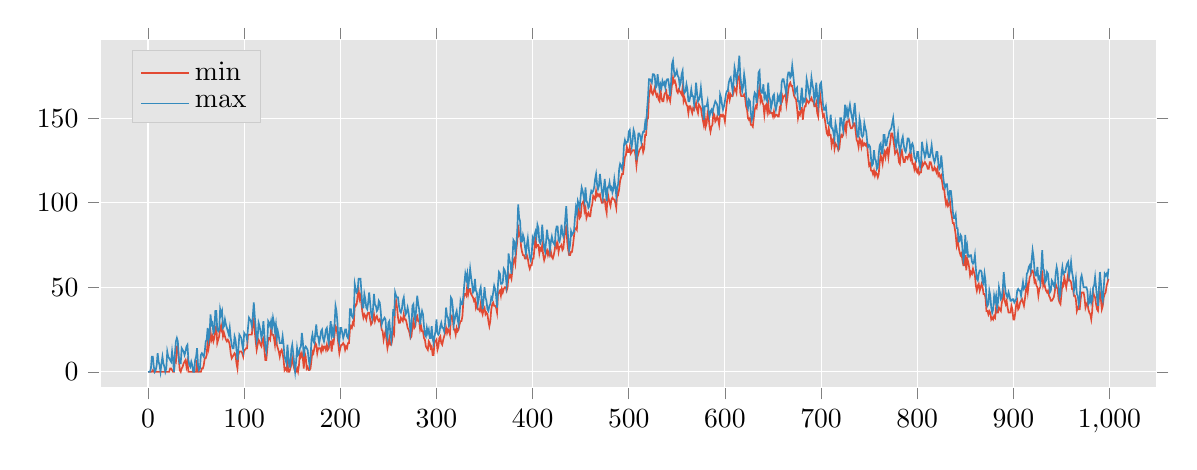
\begin{tikzpicture}

\definecolor{color1}{rgb}{0.203921568627451,0.541176470588235,0.741176470588235}
\definecolor{color0}{rgb}{0.886274509803922,0.290196078431373,0.2}

\begin{axis}[
xmin=-49.95, xmax=1048.95,
ymin=-9.35, ymax=196.35,
width=15cm,
height=6cm,
tick align=outside,
xmajorgrids,
x grid style={white},
ymajorgrids,
y grid style={white},
axis line style={white},
axis background/.style={fill=white!89.803921568627459!black},
legend cell align={left},
legend entries={{min},{max}},
legend style={at={(0.03,0.97)}, anchor=north west, draw=white!80.0!black, fill=white!89.803921568627459!black}
]
\addplot [semithick, color0]
table {%
0 0
1 0
2 0
3 0
4 0
5 1
6 0
7 0
8 0
9 0
10 0
11 0
12 0
13 0
14 0
15 0
16 0
17 0
18 0
19 0
20 0
21 0
22 0
23 2
24 2
25 1
26 0
27 0
28 7
29 6
30 15
31 15
32 8
33 1
34 0
35 2
36 3
37 5
38 6
39 7
40 3
41 6
42 0
43 0
44 0
45 0
46 0
47 0
48 0
49 0
50 0
51 7
52 0
53 0
54 0
55 0
56 2
57 2
58 4
59 8
60 8
61 10
62 18
63 14
64 18
65 24
66 19
67 21
68 18
69 20
70 26
71 27
72 17
73 19
74 21
75 27
76 25
77 28
78 21
79 23
80 21
81 19
82 18
83 19
84 18
85 16
86 11
87 8
88 9
89 10
90 11
91 10
92 5
93 2
94 10
95 12
96 12
97 12
98 11
99 9
100 13
101 13
102 14
103 14
104 22
105 22
106 22
107 22
108 22
109 29
110 31
111 24
112 18
113 13
114 16
115 19
116 18
117 16
118 15
119 19
120 20
121 13
122 7
123 7
124 13
125 20
126 20
127 19
128 25
129 22
130 22
131 20
132 16
133 23
134 16
135 14
136 12
137 9
138 12
139 13
140 11
141 7
142 1
143 2
144 1
145 6
146 0
147 0
148 2
149 4
150 8
151 5
152 2
153 0
154 0
155 2
156 0
157 4
158 11
159 9
160 11
161 8
162 2
163 11
164 9
165 2
166 3
167 1
168 1
169 2
170 7
171 12
172 11
173 14
174 17
175 16
176 11
177 14
178 14
179 14
180 12
181 15
182 13
183 15
184 15
185 13
186 16
187 13
188 14
189 18
190 18
191 12
192 18
193 17
194 22
195 27
196 26
197 22
198 16
199 11
200 14
201 16
202 16
203 17
204 16
205 13
206 15
207 14
208 17
209 17
210 25
211 27
212 26
213 29
214 28
215 40
216 39
217 40
218 45
219 49
220 43
221 45
222 40
223 35
224 32
225 34
226 33
227 31
228 34
229 35
230 35
231 31
232 28
233 29
234 31
235 34
236 30
237 32
238 33
239 31
240 30
241 31
242 29
243 25
244 24
245 19
246 22
247 24
248 19
249 14
250 17
251 20
252 16
253 16
254 19
255 25
256 23
257 40
258 42
259 38
260 32
261 29
262 29
263 32
264 31
265 30
266 34
267 31
268 31
269 29
270 26
271 25
272 23
273 20
274 21
275 27
276 30
277 26
278 27
279 32
280 33
281 30
282 30
283 25
284 27
285 24
286 24
287 20
288 19
289 15
290 14
291 13
292 18
293 17
294 14
295 15
296 10
297 10
298 18
299 18
300 19
301 13
302 15
303 20
304 21
305 17
306 16
307 19
308 21
309 23
310 26
311 23
312 25
313 24
314 22
315 32
316 33
317 31
318 25
319 25
320 22
321 26
322 24
323 25
324 28
325 30
326 30
327 33
328 42
329 46
330 46
331 45
332 51
333 46
334 49
335 49
336 46
337 45
338 44
339 42
340 43
341 38
342 40
343 37
344 37
345 36
346 40
347 36
348 34
349 37
350 38
351 34
352 35
353 34
354 30
355 27
356 30
357 37
358 40
359 41
360 39
361 39
362 38
363 35
364 46
365 47
366 48
367 45
368 49
369 47
370 49
371 50
372 50
373 48
374 50
375 58
376 56
377 57
378 55
379 60
380 66
381 67
382 64
383 72
384 77
385 87
386 81
387 82
388 74
389 71
390 69
391 69
392 67
393 67
394 69
395 67
396 63
397 61
398 63
399 63
400 67
401 67
402 74
403 80
404 74
405 75
406 75
407 70
408 73
409 72
410 75
411 69
412 66
413 68
414 71
415 72
416 69
417 71
418 69
419 71
420 68
421 67
422 69
423 72
424 77
425 74
426 76
427 71
428 74
429 74
430 75
431 72
432 73
433 79
434 85
435 86
436 77
437 72
438 69
439 69
440 71
441 71
442 75
443 80
444 85
445 85
446 84
447 94
448 96
449 91
450 92
451 99
452 100
453 101
454 95
455 97
456 91
457 93
458 94
459 92
460 92
461 97
462 99
463 104
464 103
465 102
466 107
467 104
468 105
469 104
470 105
471 102
472 100
473 100
474 102
475 102
476 97
477 94
478 106
479 103
480 100
481 98
482 102
483 103
484 102
485 102
486 100
487 97
488 106
489 105
490 108
491 113
492 115
493 117
494 117
495 122
496 127
497 128
498 133
499 130
500 130
501 133
502 129
503 130
504 131
505 131
506 131
507 128
508 122
509 127
510 129
511 131
512 132
513 133
514 134
515 130
516 132
517 140
518 140
519 149
520 150
521 163
522 166
523 169
524 165
525 164
526 166
527 168
528 165
529 163
530 164
531 161
532 160
533 167
534 162
535 160
536 160
537 164
538 165
539 166
540 161
541 163
542 162
543 160
544 165
545 170
546 174
547 171
548 172
549 170
550 166
551 165
552 167
553 166
554 165
555 164
556 168
557 160
558 162
559 160
560 158
561 157
562 153
563 157
564 157
565 155
566 153
567 156
568 155
569 157
570 159
571 155
572 153
573 158
574 157
575 156
576 152
577 149
578 146
579 151
580 145
581 147
582 153
583 151
584 145
585 142
586 145
587 146
588 153
589 152
590 148
591 149
592 151
593 149
594 146
595 152
596 152
597 151
598 152
599 151
600 148
601 154
602 159
603 163
604 165
605 161
606 164
607 163
608 163
609 165
610 168
611 167
612 165
613 172
614 174
615 175
616 165
617 163
618 163
619 163
620 164
621 162
622 157
623 155
624 150
625 149
626 150
627 146
628 146
629 145
630 150
631 155
632 157
633 156
634 161
635 165
636 168
637 160
638 162
639 159
640 158
641 152
642 157
643 158
644 154
645 159
646 153
647 154
648 153
649 153
650 151
651 154
652 151
653 152
654 152
655 151
656 151
657 156
658 155
659 165
660 161
661 163
662 163
663 164
664 158
665 162
666 167
667 170
668 171
669 169
670 169
671 166
672 163
673 162
674 161
675 156
676 150
677 153
678 152
679 156
680 156
681 149
682 154
683 157
684 157
685 161
686 160
687 159
688 160
689 161
690 162
691 160
692 160
693 157
694 157
695 159
696 153
697 151
698 161
699 164
700 159
701 155
702 151
703 152
704 149
705 145
706 141
707 140
708 144
709 140
710 140
711 134
712 137
713 138
714 132
715 135
716 134
717 133
718 131
719 132
720 138
721 140
722 139
723 140
724 144
725 146
726 142
727 148
728 148
729 149
730 146
731 144
732 144
733 145
734 147
735 147
736 142
737 137
738 136
739 133
740 138
741 137
742 133
743 136
744 134
745 135
746 134
747 135
748 133
749 127
750 122
751 123
752 119
753 119
754 117
755 119
756 116
757 118
758 117
759 115
760 117
761 124
762 128
763 126
764 123
765 128
766 130
767 127
768 131
769 132
770 127
771 132
772 136
773 141
774 141
775 138
776 134
777 129
778 130
779 131
780 129
781 124
782 123
783 130
784 131
785 127
786 124
787 124
788 127
789 127
790 126
791 128
792 129
793 126
794 128
795 123
796 123
797 120
798 123
799 119
800 118
801 120
802 117
803 118
804 118
805 124
806 122
807 123
808 124
809 123
810 122
811 120
812 120
813 124
814 124
815 122
816 119
817 119
818 121
819 120
820 118
821 120
822 116
823 117
824 115
825 116
826 112
827 108
828 108
829 103
830 99
831 101
832 98
833 99
834 101
835 95
836 92
837 88
838 88
839 85
840 81
841 75
842 78
843 74
844 71
845 69
846 70
847 66
848 63
849 63
850 69
851 60
852 67
853 65
854 62
855 57
856 59
857 58
858 61
859 59
860 57
861 51
862 48
863 51
864 52
865 48
866 50
867 52
868 50
869 46
870 46
871 44
872 36
873 36
874 34
875 36
876 35
877 31
878 32
879 31
880 33
881 32
882 38
883 35
884 35
885 38
886 37
887 36
888 41
889 43
890 47
891 42
892 40
893 42
894 38
895 35
896 35
897 35
898 39
899 37
900 31
901 31
902 35
903 40
904 42
905 37
906 38
907 41
908 42
909 43
910 41
911 39
912 43
913 48
914 52
915 47
916 52
917 56
918 57
919 60
920 60
921 58
922 53
923 54
924 51
925 50
926 45
927 49
928 50
929 55
930 60
931 51
932 53
933 50
934 48
935 47
936 48
937 45
938 44
939 42
940 42
941 43
942 44
943 47
944 52
945 50
946 49
947 43
948 41
949 40
950 46
951 52
952 51
953 56
954 53
955 50
956 54
957 58
958 54
959 54
960 53
961 49
962 49
963 45
964 45
965 43
966 36
967 38
968 37
969 37
970 43
971 47
972 47
973 47
974 44
975 38
976 40
977 41
978 37
979 35
980 34
981 31
982 36
983 47
984 45
985 44
986 40
987 37
988 36
989 43
990 47
991 43
992 37
993 39
994 44
995 46
996 47
997 51
998 53
999 55
};
\addplot [semithick, color1]
table {%
0 0
1 0
2 0
3 2
4 9
5 9
6 3
7 0
8 1
9 4
10 11
11 6
12 4
13 0
14 5
15 9
16 5
17 3
18 0
19 2
20 12
21 9
22 8
23 7
24 6
25 12
26 7
27 0
28 11
29 18
30 20
31 18
32 8
33 5
34 5
35 14
36 13
37 12
38 10
39 12
40 15
41 16
42 7
43 4
44 3
45 6
46 4
47 0
48 0
49 7
50 9
51 14
52 4
53 1
54 2
55 10
56 11
57 10
58 9
59 12
60 18
61 19
62 26
63 19
64 22
65 34
66 28
67 29
68 23
69 24
70 36
71 36
72 25
73 24
74 25
75 37
76 34
77 36
78 26
79 27
80 31
81 28
82 26
83 24
84 22
85 26
86 20
87 16
88 14
89 14
90 21
91 19
92 13
93 7
94 14
95 22
96 21
97 20
98 16
99 13
100 23
101 22
102 22
103 19
104 26
105 32
106 31
107 30
108 27
109 33
110 41
111 33
112 26
113 18
114 20
115 29
116 27
117 24
118 20
119 23
120 30
121 22
122 15
123 12
124 17
125 30
126 29
127 27
128 30
129 26
130 32
131 29
132 24
133 28
134 20
135 24
136 21
137 17
138 17
139 17
140 21
141 16
142 9
143 7
144 5
145 16
146 9
147 3
148 3
149 13
150 16
151 11
152 5
153 0
154 6
155 14
156 10
157 11
158 14
159 15
160 23
161 18
162 9
163 14
164 15
165 14
166 13
167 8
168 4
169 8
170 19
171 22
172 18
173 17
174 23
175 28
176 21
177 21
178 17
179 20
180 24
181 25
182 20
183 18
184 21
185 25
186 26
187 20
188 17
189 24
190 30
191 22
192 25
193 20
194 28
195 39
196 36
197 29
198 19
199 17
200 26
201 26
202 23
203 20
204 22
205 25
206 25
207 21
208 20
209 23
210 37
211 37
212 33
213 32
214 34
215 52
216 49
217 47
218 48
219 55
220 55
221 55
222 47
223 38
224 38
225 46
226 43
227 38
228 37
229 41
230 47
231 41
232 35
233 32
234 37
235 46
236 40
237 39
238 36
239 37
240 42
241 41
242 36
243 28
244 30
245 31
246 32
247 31
248 22
249 20
250 29
251 30
252 23
253 19
254 25
255 37
256 33
257 47
258 45
259 44
260 44
261 39
262 36
263 35
264 37
265 42
266 44
267 38
268 34
269 35
270 38
271 35
272 30
273 23
274 27
275 39
276 40
277 33
278 30
279 38
280 45
281 40
282 37
283 28
284 33
285 36
286 34
287 27
288 22
289 21
290 26
291 23
292 25
293 20
294 20
295 27
296 20
297 17
298 21
299 24
300 31
301 23
302 22
303 23
304 27
305 29
306 26
307 26
308 24
309 29
310 38
311 33
312 32
313 27
314 28
315 44
316 43
317 38
318 28
319 31
320 34
321 36
322 31
323 28
324 34
325 42
326 40
327 40
328 45
329 52
330 58
331 55
332 58
333 49
334 55
335 61
336 56
337 52
338 47
339 48
340 55
341 48
342 47
343 40
344 43
345 48
346 50
347 43
348 37
349 43
350 50
351 44
352 42
353 37
354 36
355 39
356 40
357 44
358 43
359 47
360 51
361 49
362 45
363 38
364 52
365 59
366 58
367 52
368 52
369 53
370 61
371 60
372 57
373 51
374 56
375 70
376 66
377 64
378 58
379 66
380 78
381 77
382 71
383 75
384 83
385 99
386 91
387 89
388 77
389 77
390 81
391 79
392 74
393 70
394 75
395 79
396 73
397 68
398 66
399 69
400 79
401 77
402 81
403 83
404 80
405 87
406 85
407 77
408 76
409 78
410 87
411 79
412 73
413 71
414 77
415 84
416 79
417 78
418 72
419 77
420 80
421 77
422 76
423 75
424 83
425 86
426 86
427 78
428 77
429 80
430 87
431 82
432 80
433 82
434 91
435 98
436 87
437 79
438 72
439 75
440 83
441 81
442 82
443 83
444 91
445 97
446 94
447 101
448 99
449 97
450 104
451 109
452 107
453 104
454 101
455 109
456 101
457 100
458 97
459 98
460 104
461 107
462 106
463 107
464 109
465 114
466 117
467 111
468 108
469 110
470 117
471 112
472 107
473 103
474 108
475 114
476 107
477 101
478 109
479 109
480 112
481 108
482 109
483 106
484 108
485 114
486 110
487 104
488 109
489 111
490 120
491 123
492 122
493 120
494 123
495 134
496 137
497 135
498 136
499 136
500 142
501 143
502 136
503 133
504 137
505 143
506 141
507 135
508 125
509 133
510 141
511 141
512 139
513 136
514 140
515 142
516 142
517 147
518 143
519 155
520 162
521 173
522 173
523 172
524 171
525 176
526 176
527 175
528 168
529 169
530 176
531 171
532 167
533 170
534 168
535 172
536 170
537 171
538 168
539 172
540 173
541 173
542 169
543 163
544 171
545 182
546 184
547 178
548 175
549 176
550 178
551 175
552 174
553 169
554 171
555 176
556 178
557 167
558 165
559 166
560 170
561 167
562 160
563 160
564 163
565 167
566 163
567 163
568 158
569 163
570 171
571 165
572 160
573 161
574 163
575 168
576 162
577 156
578 149
579 157
580 157
581 157
582 160
583 154
584 151
585 154
586 155
587 153
588 156
589 158
590 160
591 159
592 158
593 152
594 152
595 164
596 162
597 158
598 155
599 157
600 160
601 164
602 166
603 166
604 171
605 173
606 174
607 170
608 166
609 171
610 180
611 177
612 172
613 175
614 180
615 187
616 175
617 170
618 166
619 169
620 176
621 172
622 164
623 158
624 156
625 161
626 160
627 153
628 149
629 151
630 162
631 165
632 164
633 159
634 167
635 177
636 178
637 167
638 165
639 165
640 170
641 162
642 164
643 161
644 160
645 171
646 163
647 161
648 156
649 159
650 163
651 164
652 158
653 155
654 158
655 163
656 161
657 163
658 158
659 171
660 173
661 173
662 170
663 167
664 164
665 174
666 177
667 177
668 174
669 175
670 181
671 176
672 170
673 165
674 167
675 168
676 160
677 160
678 155
679 162
680 168
681 159
682 161
683 160
684 163
685 173
686 170
687 166
688 163
689 167
690 174
691 170
692 167
693 160
694 163
695 171
696 163
697 158
698 164
699 170
700 171
701 165
702 158
703 155
704 155
705 157
706 151
707 147
708 147
709 146
710 152
711 144
712 144
713 141
714 138
715 147
716 144
717 140
718 134
719 138
720 150
721 150
722 146
723 143
724 150
725 158
726 152
727 155
728 151
729 155
730 158
731 154
732 151
733 148
734 153
735 159
736 152
737 144
738 139
739 139
740 150
741 147
742 140
743 139
744 140
745 147
746 144
747 142
748 136
749 133
750 134
751 133
752 126
753 122
754 123
755 131
756 126
757 125
758 120
759 121
760 129
761 134
762 135
763 129
764 129
765 140
766 140
767 134
768 134
769 138
770 139
771 142
772 143
773 144
774 147
775 150
776 144
777 136
778 133
779 137
780 141
781 134
782 130
783 133
784 137
785 139
786 134
787 131
788 130
789 133
790 138
791 138
792 136
793 129
794 134
795 135
796 133
797 127
798 126
799 125
800 130
801 130
802 124
803 121
804 124
805 136
806 132
807 130
808 127
809 129
810 134
811 130
812 127
813 127
814 130
815 134
816 129
817 126
818 124
819 126
820 130
821 130
822 123
823 120
824 121
825 128
826 122
827 115
828 111
829 109
830 111
831 111
832 105
833 102
834 107
835 107
836 102
837 95
838 91
839 91
840 93
841 85
842 85
843 77
844 77
845 81
846 80
847 73
848 66
849 69
850 81
851 70
852 74
853 68
854 68
855 69
856 69
857 65
858 64
859 65
860 69
861 61
862 55
863 54
864 58
865 60
866 60
867 59
868 53
869 52
870 58
871 54
872 43
873 39
874 40
875 48
876 45
877 38
878 35
879 37
880 45
881 42
882 45
883 38
884 41
885 50
886 47
887 43
888 44
889 49
890 59
891 52
892 47
893 45
894 44
895 47
896 45
897 42
898 42
899 43
900 43
901 41
902 42
903 43
904 48
905 49
906 48
907 48
908 45
909 49
910 53
911 49
912 50
913 51
914 58
915 59
916 62
917 63
918 60
919 66
920 72
921 68
922 60
923 57
924 57
925 62
926 55
927 56
928 53
929 61
930 72
931 61
932 60
933 53
934 54
935 59
936 58
937 52
938 47
939 48
940 54
941 53
942 51
943 50
944 58
945 62
946 59
947 50
948 44
949 46
950 58
951 62
952 58
953 59
954 59
955 62
956 64
957 65
958 57
959 60
960 65
961 59
962 56
963 48
964 51
965 55
966 46
967 45
968 40
969 43
970 55
971 57
972 54
973 50
974 50
975 50
976 50
977 48
978 40
979 41
980 46
981 41
982 43
983 50
984 51
985 56
986 50
987 44
988 39
989 49
990 59
991 53
992 44
993 42
994 50
995 58
996 57
997 58
998 56
999 61
};
\end{axis}

\end{tikzpicture} 
\caption{Effect of capacity and holiday plans. We plot for each time point
  the maximum and the minimum queue length for each of the
  policies. Apparently, the effect of each of these policies is, for
  all practical purposes, negligible.  }
\label{fig:balanced}
\end{figure}


Now we consider suggestion 3, which comes down to doing more intakes
when it is busy, and do less when it is quiet. A simple rule to
implement this is by considering last week's queue $Q_{n-1}$: if
$Q_{n-1}<12$, i.e., the service capacity of one week, then do $e$
intakes less. Here, $e=1$ or $2$, or perhaps a larger number; it
corresponds to the amount of control we want to exercise. When
$Q_{n-1}>24$, i.e., larger than two weeks of intakes, do $e$ intakes
more. Let's consider three different control levels, $e=1$, $e=2$, and
$e=5$; thus in the last case all psychiatrists do one extra intake.
The previous simulation shows that it is safe to disregard the holiday
plans, so just assume a flat service capacity of 12 intakes a week.

Figure~\ref{fig:intakes} shows a striking difference indeed. The queue
does not explode any more, and already taking $e=1$ has a large
influence. 

\begin{figure}[ht]
  \centering
% progs/intake_control.py
% This file was created by matplotlib2tikz v0.5.15.
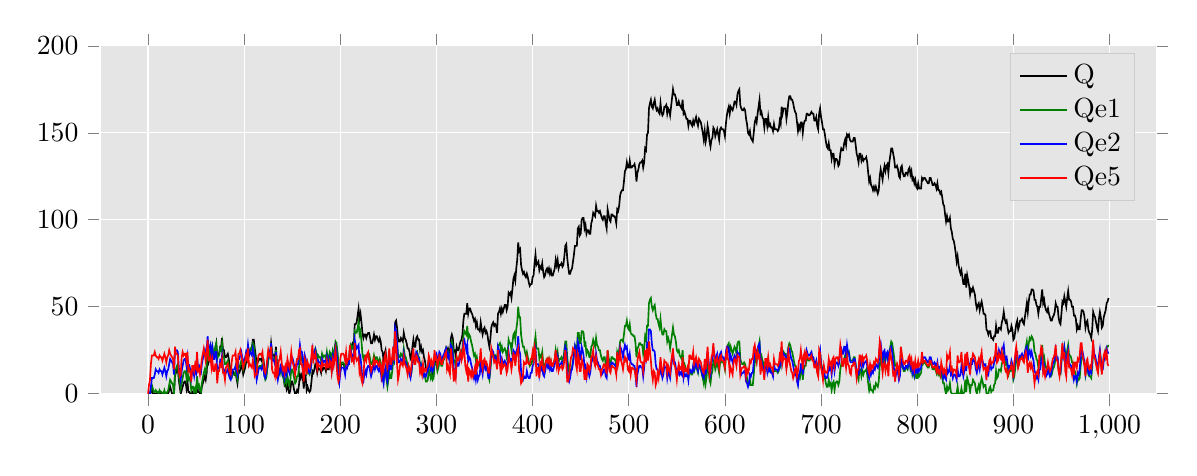
\begin{tikzpicture}

\begin{axis}[
xmin=-49.95, xmax=1048.95,
ymin=0, ymax=200,
width=15cm,
height=6cm,
tick align=outside,
xmajorgrids,
x grid style={white},
ymajorgrids,
y grid style={white},
axis line style={white},
axis background/.style={fill=white!89.803921568627459!black},
legend cell align={left},
legend entries={{Q},{Qe1},{Qe2},{Qe5}},
legend style={draw=white!80.0!black, fill=white!89.803921568627459!black}
]
\addplot [semithick, black]
table {%
0 0
1 0
2 0
3 1
4 3
5 0
6 0
7 0
8 0
9 0
10 0
11 0
12 1
13 0
14 0
15 0
16 0
17 1
18 0
19 0
20 0
21 0
22 2
23 4
24 2
25 0
26 0
27 0
28 10
29 12
30 14
31 15
32 8
33 4
34 0
35 2
36 4
37 6
38 7
39 7
40 3
41 7
42 1
43 1
44 0
45 0
46 1
47 0
48 0
49 1
50 0
51 8
52 1
53 1
54 0
55 0
56 4
57 6
58 8
59 10
60 8
61 12
62 22
63 18
64 20
65 24
66 21
67 25
68 22
69 22
70 26
71 29
72 21
73 23
74 23
75 27
76 27
77 32
78 25
79 25
80 21
81 21
82 22
83 23
84 20
85 16
86 13
87 12
88 13
89 12
90 11
91 12
92 9
93 6
94 12
95 12
96 14
97 16
98 15
99 11
100 13
101 15
102 18
103 18
104 24
105 22
106 24
107 26
108 26
109 31
110 31
111 26
112 22
113 17
114 18
115 19
116 20
117 20
118 19
119 21
120 20
121 15
122 11
123 11
124 15
125 20
126 22
127 23
128 29
129 24
130 22
131 22
132 20
133 27
134 18
135 14
136 14
137 13
138 16
139 15
140 11
141 9
142 5
143 6
144 3
145 6
146 2
147 0
148 2
149 7
150 7
151 5
152 2
153 0
154 0
155 2
156 1
157 5
158 11
159 9
160 11
161 9
162 3
163 11
164 9
165 2
166 4
167 2
168 1
169 2
170 7
171 13
172 12
173 14
174 17
175 16
176 12
177 15
178 14
179 14
180 12
181 16
182 14
183 15
184 15
185 13
186 17
187 14
188 14
189 18
190 18
191 13
192 19
193 17
194 22
195 27
196 27
197 23
198 16
199 11
200 14
201 17
202 17
203 17
204 16
205 13
206 16
207 15
208 17
209 17
210 25
211 28
212 27
213 29
214 28
215 40
216 40
217 41
218 45
219 49
220 43
221 46
222 41
223 35
224 32
225 34
226 34
227 32
228 34
229 35
230 35
231 32
232 29
233 29
234 31
235 34
236 31
237 33
238 33
239 31
240 30
241 32
242 30
243 25
244 24
245 19
246 23
247 25
248 19
249 14
250 17
251 21
252 17
253 16
254 19
255 25
256 24
257 41
258 42
259 38
260 32
261 30
262 30
263 32
264 31
265 30
266 35
267 32
268 31
269 29
270 26
271 26
272 24
273 20
274 21
275 27
276 31
277 27
278 27
279 32
280 33
281 31
282 31
283 25
284 27
285 24
286 25
287 21
288 19
289 15
290 14
291 14
292 19
293 17
294 14
295 15
296 11
297 11
298 18
299 18
300 19
301 14
302 16
303 20
304 21
305 17
306 17
307 20
308 21
309 23
310 26
311 24
312 26
313 24
314 22
315 32
316 34
317 32
318 25
319 25
320 22
321 27
322 25
323 25
324 28
325 30
326 31
327 34
328 42
329 46
330 46
331 46
332 52
333 46
334 49
335 49
336 47
337 46
338 44
339 42
340 43
341 39
342 41
343 37
344 37
345 36
346 41
347 37
348 34
349 37
350 38
351 35
352 36
353 34
354 30
355 27
356 31
357 38
358 40
359 41
360 39
361 40
362 39
363 35
364 46
365 47
366 49
367 46
368 49
369 47
370 49
371 51
372 51
373 48
374 50
375 58
376 57
377 58
378 55
379 60
380 66
381 68
382 65
383 72
384 77
385 87
386 82
387 83
388 74
389 71
390 69
391 70
392 68
393 67
394 69
395 67
396 64
397 62
398 63
399 63
400 67
401 68
402 75
403 80
404 74
405 75
406 76
407 71
408 73
409 72
410 75
411 70
412 67
413 68
414 71
415 72
416 70
417 72
418 69
419 71
420 68
421 68
422 70
423 72
424 77
425 74
426 77
427 72
428 74
429 74
430 75
431 73
432 74
433 79
434 85
435 86
436 78
437 73
438 69
439 69
440 71
441 72
442 76
443 80
444 85
445 85
446 85
447 95
448 96
449 91
450 92
451 100
452 101
453 101
454 95
455 97
456 92
457 94
458 94
459 92
460 92
461 98
462 100
463 104
464 103
465 102
466 108
467 105
468 105
469 104
470 105
471 103
472 101
473 100
474 102
475 102
476 98
477 95
478 106
479 103
480 100
481 99
482 103
483 103
484 102
485 102
486 101
487 98
488 106
489 105
490 108
491 114
492 116
493 117
494 117
495 122
496 128
497 129
498 133
499 130
500 130
501 134
502 130
503 130
504 131
505 131
506 132
507 129
508 122
509 127
510 129
511 132
512 133
513 133
514 134
515 130
516 133
517 141
518 140
519 149
520 150
521 164
522 167
523 169
524 165
525 164
526 167
527 169
528 165
529 163
530 164
531 162
532 161
533 167
534 162
535 160
536 161
537 165
538 165
539 166
540 161
541 164
542 163
543 160
544 165
545 170
546 175
547 172
548 172
549 170
550 166
551 166
552 168
553 166
554 165
555 164
556 169
557 161
558 162
559 160
560 158
561 158
562 154
563 157
564 157
565 155
566 154
567 157
568 155
569 157
570 159
571 156
572 154
573 158
574 157
575 156
576 153
577 150
578 146
579 151
580 145
581 148
582 154
583 151
584 145
585 142
586 146
587 147
588 153
589 152
590 148
591 150
592 152
593 149
594 146
595 152
596 153
597 152
598 152
599 151
600 148
601 155
602 160
603 163
604 165
605 161
606 165
607 164
608 163
609 165
610 168
611 168
612 166
613 172
614 174
615 175
616 166
617 164
618 163
619 163
620 164
621 163
622 158
623 155
624 150
625 149
626 151
627 147
628 146
629 145
630 150
631 156
632 158
633 156
634 161
635 165
636 169
637 161
638 162
639 159
640 158
641 153
642 158
643 158
644 154
645 159
646 154
647 155
648 153
649 153
650 151
651 155
652 152
653 152
654 152
655 151
656 152
657 157
658 155
659 165
660 161
661 164
662 164
663 164
664 158
665 162
666 168
667 171
668 171
669 169
670 169
671 167
672 164
673 162
674 161
675 156
676 151
677 154
678 152
679 156
680 156
681 150
682 155
683 157
684 157
685 161
686 161
687 160
688 160
689 161
690 162
691 161
692 161
693 157
694 157
695 159
696 154
697 152
698 161
699 164
700 159
701 156
702 152
703 152
704 149
705 145
706 142
707 141
708 144
709 140
710 140
711 135
712 138
713 138
714 132
715 135
716 135
717 134
718 131
719 132
720 138
721 141
722 140
723 140
724 144
725 146
726 143
727 149
728 148
729 149
730 146
731 145
732 145
733 145
734 147
735 147
736 143
737 138
738 136
739 133
740 138
741 138
742 134
743 136
744 134
745 135
746 135
747 136
748 133
749 127
750 122
751 124
752 120
753 119
754 117
755 119
756 117
757 119
758 117
759 115
760 117
761 125
762 129
763 126
764 123
765 128
766 131
767 128
768 131
769 132
770 127
771 133
772 137
773 141
774 141
775 138
776 135
777 130
778 130
779 131
780 129
781 125
782 124
783 130
784 131
785 127
786 125
787 125
788 127
789 127
790 126
791 129
792 130
793 126
794 128
795 123
796 124
797 121
798 123
799 119
800 118
801 121
802 118
803 118
804 118
805 124
806 123
807 124
808 124
809 123
810 122
811 121
812 121
813 124
814 124
815 122
816 120
817 120
818 121
819 120
820 118
821 121
822 117
823 117
824 115
825 116
826 113
827 109
828 108
829 103
830 99
831 102
832 99
833 99
834 101
835 95
836 93
837 89
838 88
839 85
840 81
841 76
842 79
843 74
844 71
845 69
846 71
847 67
848 63
849 63
850 69
851 61
852 68
853 65
854 62
855 57
856 60
857 59
858 61
859 59
860 57
861 52
862 49
863 51
864 52
865 48
866 51
867 53
868 50
869 46
870 46
871 45
872 37
873 36
874 34
875 36
876 36
877 32
878 32
879 31
880 33
881 33
882 39
883 35
884 35
885 38
886 38
887 37
888 41
889 43
890 47
891 43
892 41
893 42
894 38
895 35
896 36
897 36
898 39
899 37
900 31
901 32
902 36
903 40
904 42
905 37
906 39
907 42
908 42
909 43
910 41
911 40
912 44
913 48
914 52
915 47
916 53
917 57
918 57
919 60
920 60
921 59
922 54
923 54
924 51
925 50
926 46
927 50
928 50
929 55
930 60
931 52
932 54
933 50
934 48
935 47
936 49
937 46
938 44
939 42
940 42
941 44
942 45
943 47
944 52
945 50
946 50
947 44
948 41
949 40
950 46
951 53
952 52
953 56
954 53
955 50
956 55
957 59
958 54
959 54
960 53
961 50
962 50
963 45
964 45
965 43
966 37
967 39
968 37
969 37
970 43
971 48
972 48
973 47
974 44
975 38
976 41
977 42
978 37
979 35
980 34
981 32
982 37
983 47
984 45
985 44
986 41
987 38
988 36
989 43
990 47
991 44
992 38
993 39
994 44
995 46
996 48
997 52
998 53
999 55
};
\addplot [semithick, green!50.196078431372548!black]
table {%
0 0
1 0
2 0
3 2
4 5
5 3
6 1
7 1
8 2
9 1
10 1
11 0
12 2
13 1
14 1
15 0
16 0
17 2
18 0
19 0
20 1
21 2
22 5
23 8
24 7
25 6
26 5
27 0
28 11
29 14
30 16
31 17
32 10
33 7
34 3
35 6
36 9
37 12
38 13
39 13
40 9
41 14
42 8
43 9
44 7
45 2
46 4
47 4
48 1
49 3
50 1
51 10
52 4
53 5
54 2
55 1
56 6
57 9
58 12
59 14
60 12
61 16
62 26
63 21
64 23
65 27
66 23
67 27
68 23
69 23
70 27
71 29
72 20
73 22
74 22
75 26
76 25
77 29
78 21
79 21
80 17
81 17
82 18
83 19
84 16
85 12
86 9
87 9
88 11
89 11
90 11
91 13
92 10
93 8
94 15
95 15
96 17
97 19
98 18
99 14
100 16
101 18
102 21
103 21
104 27
105 24
106 25
107 26
108 25
109 29
110 28
111 22
112 18
113 13
114 14
115 15
116 16
117 16
118 15
119 17
120 16
121 11
122 8
123 9
124 14
125 19
126 21
127 22
128 28
129 22
130 20
131 20
132 18
133 25
134 15
135 11
136 12
137 11
138 15
139 14
140 10
141 9
142 6
143 8
144 6
145 10
146 7
147 5
148 8
149 14
150 14
151 12
152 9
153 6
154 7
155 10
156 10
157 15
158 21
159 19
160 21
161 19
162 13
163 21
164 19
165 12
166 14
167 12
168 11
169 13
170 18
171 24
172 22
173 24
174 26
175 24
176 19
177 22
178 21
179 21
180 19
181 23
182 21
183 22
184 22
185 20
186 24
187 20
188 20
189 24
190 23
191 18
192 24
193 21
194 26
195 30
196 29
197 24
198 16
199 11
200 15
201 18
202 18
203 18
204 17
205 14
206 17
207 16
208 18
209 18
210 26
211 28
212 26
213 27
214 25
215 36
216 35
217 35
218 38
219 41
220 34
221 36
222 30
223 23
224 20
225 22
226 22
227 20
228 22
229 23
230 23
231 20
232 17
233 17
234 19
235 22
236 19
237 21
238 21
239 19
240 18
241 20
242 18
243 13
244 12
245 7
246 12
247 14
248 8
249 4
250 8
251 13
252 9
253 9
254 13
255 19
256 18
257 35
258 35
259 30
260 23
261 21
262 21
263 23
264 22
265 21
266 26
267 22
268 21
269 19
270 16
271 16
272 14
273 10
274 12
275 18
276 22
277 18
278 18
279 23
280 24
281 21
282 21
283 15
284 17
285 14
286 15
287 11
288 10
289 7
290 7
291 8
292 14
293 12
294 9
295 11
296 8
297 9
298 17
299 17
300 18
301 13
302 15
303 19
304 20
305 16
306 16
307 19
308 20
309 22
310 25
311 22
312 24
313 21
314 19
315 29
316 30
317 27
318 19
319 19
320 16
321 21
322 19
323 19
324 22
325 24
326 24
327 26
328 33
329 36
330 35
331 34
332 39
333 32
334 34
335 33
336 30
337 28
338 25
339 22
340 23
341 19
342 21
343 17
344 17
345 16
346 21
347 17
348 14
349 17
350 18
351 15
352 16
353 14
354 10
355 8
356 13
357 20
358 22
359 23
360 21
361 22
362 21
363 17
364 28
365 28
366 29
367 25
368 27
369 24
370 25
371 26
372 25
373 21
374 23
375 31
376 29
377 29
378 25
379 29
380 34
381 35
382 31
383 37
384 41
385 50
386 44
387 44
388 34
389 30
390 27
391 27
392 24
393 22
394 24
395 21
396 18
397 16
398 17
399 17
400 21
401 22
402 29
403 33
404 26
405 26
406 26
407 20
408 22
409 21
410 24
411 18
412 15
413 16
414 19
415 20
416 18
417 20
418 17
419 19
420 16
421 16
422 18
423 20
424 25
425 21
426 24
427 18
428 20
429 20
430 21
431 19
432 20
433 25
434 30
435 30
436 21
437 16
438 12
439 12
440 14
441 15
442 19
443 23
444 28
445 27
446 26
447 35
448 35
449 29
450 29
451 36
452 36
453 35
454 28
455 29
456 23
457 25
458 24
459 21
460 21
461 27
462 28
463 31
464 29
465 27
466 32
467 28
468 27
469 25
470 25
471 22
472 20
473 19
474 21
475 21
476 17
477 14
478 25
479 21
480 18
481 17
482 21
483 21
484 20
485 20
486 19
487 16
488 24
489 22
490 25
491 30
492 31
493 31
494 30
495 34
496 39
497 39
498 42
499 38
500 37
501 40
502 35
503 34
504 34
505 33
506 33
507 29
508 21
509 26
510 27
511 29
512 29
513 28
514 28
515 23
516 26
517 33
518 31
519 39
520 39
521 52
522 54
523 55
524 50
525 48
526 50
527 51
528 46
529 43
530 43
531 40
532 38
533 43
534 37
535 34
536 34
537 37
538 36
539 36
540 30
541 32
542 30
543 26
544 30
545 34
546 38
547 34
548 33
549 30
550 25
551 24
552 25
553 22
554 21
555 20
556 25
557 16
558 17
559 15
560 13
561 13
562 9
563 13
564 13
565 11
566 11
567 15
568 13
569 15
570 17
571 14
572 12
573 16
574 15
575 14
576 11
577 9
578 6
579 12
580 6
581 10
582 17
583 14
584 8
585 6
586 11
587 13
588 19
589 18
590 14
591 16
592 18
593 15
594 12
595 18
596 19
597 18
598 18
599 17
600 14
601 21
602 26
603 28
604 29
605 24
606 27
607 25
608 23
609 25
610 27
611 26
612 23
613 29
614 30
615 30
616 20
617 18
618 17
619 17
620 18
621 17
622 12
623 9
624 5
625 5
626 8
627 5
628 5
629 5
630 11
631 18
632 20
633 18
634 23
635 27
636 30
637 21
638 22
639 19
640 18
641 13
642 18
643 18
644 14
645 19
646 14
647 15
648 13
649 13
650 11
651 16
652 13
653 13
654 13
655 12
656 13
657 18
658 16
659 26
660 21
661 24
662 23
663 23
664 17
665 21
666 27
667 29
668 28
669 25
670 24
671 21
672 18
673 16
674 15
675 10
676 6
677 10
678 9
679 14
680 14
681 8
682 14
683 16
684 16
685 20
686 20
687 19
688 19
689 20
690 21
691 20
692 20
693 16
694 16
695 18
696 13
697 11
698 21
699 24
700 18
701 15
702 11
703 12
704 9
705 6
706 4
707 4
708 8
709 5
710 6
711 2
712 6
713 7
714 2
715 6
716 7
717 7
718 5
719 7
720 14
721 17
722 16
723 16
724 20
725 22
726 19
727 25
728 23
729 24
730 20
731 19
732 19
733 19
734 21
735 21
736 17
737 12
738 10
739 8
740 14
741 14
742 10
743 13
744 11
745 13
746 13
747 14
748 11
749 6
750 2
751 5
752 2
753 2
754 1
755 4
756 3
757 6
758 5
759 4
760 7
761 16
762 20
763 17
764 14
765 19
766 22
767 19
768 22
769 23
770 18
771 24
772 27
773 30
774 29
775 25
776 21
777 16
778 16
779 17
780 15
781 11
782 11
783 18
784 19
785 15
786 13
787 13
788 15
789 15
790 14
791 17
792 18
793 14
794 16
795 11
796 13
797 10
798 13
799 9
800 9
801 13
802 10
803 11
804 12
805 18
806 17
807 18
808 18
809 17
810 16
811 15
812 15
813 18
814 18
815 16
816 14
817 14
818 15
819 14
820 12
821 15
822 11
823 12
824 10
825 12
826 9
827 6
828 6
829 2
830 0
831 4
832 2
833 3
834 6
835 1
836 0
837 0
838 0
839 0
840 0
841 0
842 4
843 0
844 0
845 0
846 3
847 0
848 0
849 1
850 8
851 1
852 9
853 7
854 5
855 1
856 5
857 5
858 8
859 7
860 6
861 2
862 0
863 3
864 5
865 2
866 6
867 9
868 7
869 4
870 5
871 5
872 0
873 0
874 0
875 3
876 4
877 1
878 2
879 2
880 5
881 6
882 13
883 9
884 10
885 14
886 14
887 13
888 17
889 19
890 23
891 19
892 17
893 18
894 14
895 11
896 13
897 13
898 16
899 14
900 8
901 10
902 15
903 19
904 21
905 16
906 18
907 21
908 21
909 22
910 20
911 19
912 23
913 27
914 30
915 24
916 29
917 32
918 31
919 33
920 32
921 30
922 24
923 23
924 20
925 19
926 15
927 19
928 19
929 24
930 28
931 19
932 21
933 17
934 15
935 14
936 16
937 13
938 11
939 10
940 11
941 14
942 15
943 17
944 22
945 20
946 20
947 14
948 11
949 11
950 18
951 25
952 23
953 27
954 23
955 20
956 25
957 28
958 22
959 22
960 21
961 18
962 18
963 13
964 13
965 11
966 6
967 9
968 8
969 9
970 16
971 21
972 21
973 20
974 17
975 11
976 15
977 16
978 11
979 10
980 10
981 9
982 15
983 25
984 22
985 21
986 18
987 15
988 13
989 20
990 24
991 20
992 14
993 15
994 20
995 22
996 24
997 27
998 27
999 28
};
\addplot [semithick, blue]
table {%
0 0
1 0
2 0
3 4
4 9
5 9
6 9
7 11
8 14
9 13
10 13
11 12
12 14
13 13
14 13
15 11
16 13
17 15
18 13
19 10
20 13
21 14
22 17
23 20
24 19
25 18
26 17
27 11
28 24
29 25
30 25
31 24
32 15
33 12
34 8
35 13
36 16
37 19
38 20
39 20
40 16
41 21
42 15
43 16
44 14
45 9
46 13
47 13
48 10
49 14
50 12
51 21
52 15
53 16
54 13
55 12
56 17
57 20
58 23
59 25
60 21
61 25
62 33
63 26
64 26
65 28
66 22
67 26
68 20
69 20
70 24
71 24
72 13
73 15
74 15
75 19
76 18
77 22
78 14
79 14
80 10
81 12
82 13
83 14
84 11
85 9
86 8
87 10
88 14
89 14
90 14
91 16
92 13
93 11
94 20
95 20
96 22
97 24
98 21
99 17
100 19
101 21
102 24
103 22
104 28
105 23
106 24
107 23
108 22
109 26
110 23
111 17
112 13
113 8
114 11
115 14
116 15
117 15
118 14
119 16
120 15
121 10
122 9
123 12
124 17
125 22
126 24
127 23
128 29
129 21
130 19
131 19
132 17
133 24
134 12
135 8
136 11
137 12
138 16
139 15
140 11
141 12
142 9
143 13
144 11
145 17
146 14
147 12
148 15
149 21
150 21
151 19
152 16
153 13
154 14
155 17
156 17
157 22
158 28
159 24
160 24
161 20
162 14
163 22
164 20
165 13
166 15
167 13
168 12
169 14
170 19
171 25
172 21
173 23
174 25
175 21
176 16
177 19
178 18
179 18
180 16
181 20
182 18
183 19
184 19
185 17
186 21
187 17
188 17
189 21
190 20
191 15
192 21
193 18
194 23
195 27
196 24
197 17
198 9
199 6
200 12
201 15
202 15
203 15
204 14
205 11
206 16
207 15
208 17
209 17
210 25
211 25
212 21
213 22
214 20
215 31
216 28
217 26
218 27
219 28
220 19
221 21
222 15
223 8
224 7
225 11
226 13
227 11
228 15
229 16
230 16
231 13
232 10
233 12
234 14
235 17
236 14
237 16
238 16
239 14
240 13
241 15
242 13
243 8
244 9
245 6
246 13
247 15
248 9
249 7
250 13
251 18
252 14
253 14
254 18
255 24
256 21
257 38
258 36
259 29
260 20
261 18
262 18
263 20
264 19
265 18
266 23
267 19
268 18
269 16
270 13
271 13
272 11
273 9
274 13
275 19
276 23
277 19
278 19
279 24
280 23
281 20
282 20
283 14
284 16
285 13
286 14
287 10
288 11
289 10
290 12
291 13
292 19
293 17
294 14
295 16
296 13
297 14
298 22
299 22
300 23
301 18
302 20
303 24
304 23
305 19
306 19
307 22
308 23
309 25
310 26
311 21
312 23
313 20
314 18
315 28
316 27
317 22
318 14
319 14
320 11
321 18
322 16
323 16
324 19
325 21
326 21
327 23
328 30
329 31
330 28
331 25
332 28
333 19
334 21
335 20
336 17
337 15
338 12
339 9
340 12
341 8
342 12
343 8
344 10
345 11
346 18
347 14
348 11
349 16
350 17
351 14
352 15
353 13
354 9
355 9
356 16
357 23
358 25
359 24
360 20
361 21
362 20
363 16
364 27
365 25
366 24
367 18
368 20
369 17
370 18
371 19
372 18
373 14
374 16
375 24
376 20
377 20
378 16
379 20
380 25
381 24
382 18
383 24
384 26
385 33
386 25
387 23
388 13
389 9
390 8
391 10
392 9
393 9
394 13
395 10
396 9
397 9
398 12
399 12
400 16
401 17
402 24
403 26
404 17
405 17
406 17
407 11
408 15
409 14
410 17
411 11
412 10
413 13
414 16
415 17
416 15
417 17
418 14
419 16
420 13
421 13
422 15
423 17
424 22
425 18
426 21
427 15
428 17
429 17
430 18
431 16
432 17
433 22
434 27
435 25
436 14
437 9
438 7
439 9
440 13
441 14
442 18
443 22
444 27
445 24
446 21
447 30
448 28
449 20
450 20
451 27
452 25
453 22
454 15
455 16
456 10
457 14
458 13
459 10
460 12
461 18
462 19
463 22
464 20
465 18
466 23
467 19
468 18
469 16
470 16
471 13
472 11
473 12
474 14
475 14
476 10
477 9
478 22
479 18
480 15
481 14
482 18
483 18
484 17
485 17
486 16
487 13
488 21
489 19
490 22
491 27
492 26
493 24
494 21
495 25
496 28
497 26
498 27
499 21
500 20
501 23
502 18
503 17
504 17
505 16
506 16
507 12
508 4
509 11
510 14
511 16
512 16
513 15
514 15
515 10
516 15
517 22
518 20
519 28
520 26
521 37
522 37
523 36
524 29
525 25
526 25
527 24
528 17
529 14
530 14
531 11
532 11
533 18
534 12
535 9
536 11
537 16
538 15
539 15
540 9
541 13
542 11
543 9
544 15
545 19
546 23
547 19
548 18
549 15
550 10
551 11
552 14
553 11
554 12
555 11
556 18
557 9
558 12
559 10
560 10
561 12
562 8
563 14
564 14
565 12
566 12
567 16
568 14
569 16
570 18
571 15
572 13
573 17
574 16
575 15
576 12
577 10
578 9
579 17
580 11
581 17
582 24
583 19
584 13
585 11
586 18
587 20
588 26
589 23
590 19
591 21
592 23
593 20
594 17
595 23
596 24
597 21
598 21
599 20
600 17
601 24
602 27
603 27
604 26
605 19
606 22
607 20
608 18
609 20
610 22
611 21
612 18
613 24
614 23
615 23
616 13
617 11
618 12
619 12
620 13
621 12
622 7
623 6
624 4
625 6
626 11
627 10
628 12
629 12
630 18
631 25
632 25
633 21
634 26
635 28
636 29
637 18
638 19
639 16
640 15
641 10
642 17
643 17
644 13
645 18
646 13
647 14
648 12
649 12
650 10
651 17
652 14
653 14
654 14
655 13
656 14
657 19
658 17
659 27
660 20
661 23
662 22
663 22
664 16
665 20
666 26
667 26
668 23
669 20
670 19
671 16
672 13
673 11
674 12
675 7
676 5
677 11
678 12
679 17
680 17
681 11
682 19
683 21
684 21
685 25
686 23
687 22
688 22
689 23
690 24
691 21
692 21
693 17
694 17
695 19
696 14
697 12
698 22
699 25
700 17
701 14
702 10
703 13
704 10
705 9
706 9
707 11
708 17
709 14
710 15
711 11
712 17
713 18
714 13
715 17
716 18
717 18
718 16
719 18
720 25
721 26
722 23
723 23
724 27
725 27
726 22
727 28
728 24
729 23
730 19
731 18
732 18
733 18
734 20
735 20
736 16
737 11
738 11
739 11
740 19
741 19
742 15
743 18
744 16
745 18
746 18
747 19
748 16
749 11
750 9
751 14
752 11
753 13
754 12
755 15
756 14
757 17
758 16
759 15
760 18
761 27
762 29
763 24
764 19
765 24
766 25
767 20
768 23
769 24
770 17
771 23
772 26
773 27
774 24
775 18
776 14
777 9
778 11
779 14
780 12
781 8
782 10
783 19
784 20
785 16
786 14
787 14
788 16
789 16
790 15
791 18
792 19
793 15
794 17
795 12
796 14
797 11
798 16
799 12
800 12
801 16
802 13
803 14
804 15
805 21
806 20
807 21
808 21
809 20
810 19
811 18
812 18
813 21
814 21
815 19
816 17
817 17
818 18
819 17
820 15
821 18
822 14
823 15
824 13
825 15
826 12
827 9
828 11
829 9
830 8
831 14
832 12
833 13
834 16
835 11
836 12
837 9
838 11
839 11
840 10
841 8
842 14
843 10
844 10
845 11
846 16
847 13
848 10
849 13
850 20
851 13
852 21
853 19
854 17
855 13
856 17
857 17
858 20
859 19
860 18
861 14
862 12
863 15
864 17
865 14
866 18
867 21
868 19
869 16
870 17
871 17
872 10
873 12
874 11
875 16
876 17
877 14
878 15
879 15
880 18
881 19
882 26
883 20
884 21
885 25
886 23
887 22
888 26
889 26
890 28
891 22
892 20
893 21
894 17
895 14
896 16
897 16
898 19
899 17
900 11
901 15
902 20
903 24
904 24
905 17
906 19
907 22
908 22
909 23
910 21
911 20
912 24
913 26
914 27
915 19
916 24
917 25
918 22
919 24
920 21
921 19
922 13
923 12
924 9
925 10
926 8
927 14
928 14
929 19
930 23
931 14
932 16
933 12
934 10
935 11
936 15
937 12
938 10
939 11
940 14
941 17
942 18
943 20
944 25
945 21
946 21
947 15
948 12
949 12
950 19
951 26
952 22
953 26
954 20
955 17
956 22
957 25
958 17
959 17
960 16
961 13
962 13
963 8
964 10
965 10
966 7
967 12
968 11
969 14
970 21
971 26
972 24
973 21
974 18
975 12
976 16
977 17
978 12
979 11
980 13
981 12
982 18
983 28
984 23
985 22
986 19
987 16
988 14
989 21
990 25
991 19
992 13
993 14
994 19
995 21
996 23
997 26
998 24
999 23
};
\addplot [semithick, red]
table {%
0 0
1 5
2 8
3 17
4 22
5 22
6 22
7 24
8 22
9 21
10 21
11 20
12 22
13 21
14 21
15 19
16 21
17 23
18 21
19 18
20 21
21 22
22 25
23 23
24 22
25 21
26 20
27 14
28 27
29 23
30 23
31 22
32 13
33 10
34 11
35 21
36 24
37 22
38 23
39 23
40 19
41 24
42 13
43 14
44 12
45 7
46 16
47 16
48 13
49 17
50 15
51 24
52 13
53 14
54 11
55 15
56 20
57 23
58 26
59 23
60 19
61 23
62 31
63 19
64 19
65 21
66 15
67 19
68 13
69 13
70 17
71 17
72 6
73 13
74 13
75 17
76 16
77 20
78 12
79 12
80 8
81 15
82 16
83 17
84 14
85 12
86 11
87 18
88 22
89 22
90 22
91 24
92 16
93 14
94 23
95 23
96 25
97 22
98 19
99 15
100 17
101 19
102 22
103 20
104 26
105 16
106 17
107 16
108 15
109 19
110 16
111 10
112 11
113 11
114 19
115 22
116 23
117 23
118 22
119 24
120 18
121 13
122 12
123 15
124 20
125 25
126 22
127 21
128 27
129 14
130 12
131 12
132 10
133 22
134 10
135 11
136 19
137 20
138 24
139 18
140 14
141 15
142 12
143 16
144 14
145 20
146 17
147 15
148 18
149 24
150 19
151 17
152 14
153 11
154 17
155 20
156 20
157 25
158 26
159 17
160 17
161 13
162 7
163 20
164 18
165 11
166 18
167 16
168 15
169 17
170 22
171 28
172 19
173 21
174 23
175 19
176 14
177 17
178 16
179 16
180 14
181 18
182 16
183 17
184 17
185 15
186 19
187 15
188 15
189 19
190 18
191 13
192 19
193 16
194 21
195 25
196 17
197 10
198 7
199 9
200 20
201 23
202 23
203 23
204 22
205 19
206 24
207 18
208 20
209 20
210 28
211 23
212 19
213 20
214 18
215 29
216 21
217 19
218 20
219 21
220 12
221 14
222 8
223 6
224 10
225 19
226 21
227 19
228 23
229 24
230 19
231 16
232 13
233 15
234 17
235 20
236 17
237 19
238 19
239 17
240 16
241 18
242 16
243 11
244 17
245 14
246 21
247 23
248 17
249 15
250 21
251 26
252 17
253 17
254 21
255 27
256 19
257 36
258 29
259 17
260 8
261 11
262 16
263 18
264 17
265 16
266 21
267 17
268 16
269 14
270 11
271 16
272 14
273 12
274 16
275 22
276 26
277 17
278 17
279 22
280 21
281 18
282 18
283 12
284 14
285 11
286 17
287 13
288 14
289 13
290 15
291 16
292 22
293 20
294 17
295 19
296 16
297 17
298 25
299 20
300 21
301 16
302 18
303 22
304 21
305 17
306 17
307 20
308 21
309 23
310 24
311 14
312 16
313 13
314 11
315 26
316 20
317 15
318 7
319 12
320 9
321 21
322 19
323 19
324 22
325 24
326 19
327 21
328 28
329 24
330 16
331 13
332 16
333 7
334 14
335 13
336 10
337 13
338 10
339 12
340 15
341 11
342 20
343 16
344 18
345 19
346 26
347 17
348 14
349 19
350 20
351 17
352 18
353 16
354 12
355 12
356 19
357 26
358 23
359 22
360 18
361 19
362 18
363 14
364 25
365 18
366 17
367 11
368 18
369 15
370 16
371 17
372 16
373 12
374 14
375 22
376 18
377 18
378 14
379 18
380 23
381 22
382 16
383 22
384 24
385 26
386 13
387 11
388 6
389 7
390 11
391 18
392 17
393 17
394 21
395 18
396 17
397 17
398 20
399 20
400 24
401 20
402 27
403 24
404 10
405 15
406 15
407 9
408 18
409 17
410 20
411 14
412 13
413 16
414 19
415 20
416 18
417 20
418 17
419 19
420 16
421 16
422 18
423 20
424 25
425 16
426 19
427 13
428 15
429 15
430 16
431 14
432 15
433 20
434 25
435 18
436 7
437 7
438 10
439 17
440 21
441 22
442 26
443 25
444 25
445 17
446 14
447 23
448 21
449 13
450 13
451 20
452 18
453 15
454 8
455 14
456 8
457 17
458 16
459 13
460 15
461 21
462 22
463 25
464 18
465 16
466 21
467 17
468 16
469 14
470 14
471 11
472 14
473 15
474 17
475 17
476 13
477 12
478 25
479 16
480 13
481 12
482 16
483 16
484 15
485 15
486 14
487 11
488 24
489 17
490 20
491 25
492 19
493 17
494 14
495 18
496 21
497 19
498 20
499 14
500 13
501 16
502 11
503 15
504 15
505 14
506 14
507 10
508 7
509 19
510 22
511 24
512 19
513 18
514 18
515 13
516 18
517 25
518 18
519 26
520 19
521 30
522 25
523 19
524 12
525 8
526 13
527 12
528 5
529 7
530 12
531 9
532 14
533 21
534 15
535 12
536 14
537 19
538 18
539 18
540 12
541 16
542 14
543 12
544 18
545 22
546 26
547 17
548 16
549 13
550 8
551 14
552 17
553 14
554 15
555 14
556 21
557 12
558 15
559 13
560 13
561 15
562 11
563 22
564 22
565 20
566 20
567 24
568 17
569 19
570 21
571 18
572 16
573 20
574 19
575 18
576 15
577 13
578 12
579 20
580 14
581 20
582 27
583 17
584 11
585 14
586 21
587 23
588 29
589 21
590 17
591 19
592 21
593 18
594 15
595 21
596 22
597 19
598 19
599 18
600 15
601 22
602 25
603 20
604 19
605 12
606 15
607 13
608 11
609 18
610 20
611 19
612 16
613 22
614 21
615 21
616 11
617 14
618 15
619 15
620 16
621 15
622 10
623 14
624 12
625 14
626 19
627 18
628 20
629 20
630 26
631 28
632 23
633 19
634 24
635 21
636 22
637 11
638 17
639 14
640 13
641 8
642 20
643 20
644 16
645 21
646 16
647 17
648 15
649 15
650 13
651 20
652 17
653 17
654 17
655 16
656 17
657 22
658 20
659 30
660 18
661 21
662 20
663 20
664 14
665 18
666 24
667 19
668 16
669 13
670 12
671 9
672 11
673 14
674 15
675 10
676 13
677 19
678 20
679 25
680 20
681 14
682 22
683 24
684 19
685 23
686 21
687 20
688 20
689 21
690 22
691 19
692 19
693 15
694 15
695 17
696 12
697 10
698 25
699 23
700 15
701 12
702 8
703 16
704 13
705 12
706 12
707 14
708 20
709 17
710 18
711 14
712 20
713 21
714 16
715 20
716 21
717 21
718 19
719 21
720 28
721 24
722 16
723 16
724 20
725 20
726 15
727 21
728 17
729 16
730 12
731 11
732 16
733 16
734 18
735 18
736 14
737 9
738 14
739 14
740 22
741 22
742 18
743 21
744 19
745 21
746 21
747 22
748 19
749 14
750 12
751 17
752 14
753 16
754 15
755 18
756 17
757 20
758 19
759 18
760 21
761 30
762 27
763 17
764 12
765 17
766 18
767 13
768 16
769 17
770 10
771 21
772 24
773 20
774 17
775 11
776 12
777 7
778 14
779 17
780 15
781 11
782 18
783 27
784 23
785 19
786 17
787 17
788 19
789 19
790 18
791 21
792 22
793 18
794 20
795 15
796 17
797 14
798 19
799 15
800 15
801 19
802 16
803 17
804 18
805 24
806 18
807 19
808 19
809 18
810 17
811 16
812 16
813 19
814 19
815 17
816 15
817 15
818 16
819 15
820 13
821 16
822 12
823 13
824 11
825 18
826 15
827 12
828 14
829 12
830 11
831 22
832 20
833 21
834 24
835 14
836 15
837 12
838 14
839 14
840 13
841 11
842 22
843 18
844 18
845 19
846 24
847 16
848 13
849 16
850 23
851 16
852 24
853 17
854 15
855 11
856 20
857 20
858 23
859 22
860 21
861 17
862 15
863 18
864 20
865 17
866 21
867 24
868 17
869 14
870 15
871 15
872 8
873 15
874 14
875 19
876 20
877 17
878 18
879 18
880 21
881 22
882 29
883 18
884 19
885 23
886 21
887 20
888 24
889 19
890 21
891 15
892 13
893 14
894 10
895 12
896 14
897 14
898 17
899 15
900 9
901 18
902 23
903 27
904 22
905 15
906 17
907 20
908 20
909 21
910 19
911 18
912 22
913 24
914 20
915 12
916 17
917 18
918 15
919 17
920 14
921 12
922 6
923 10
924 12
925 13
926 11
927 22
928 22
929 27
930 26
931 12
932 14
933 10
934 13
935 14
936 18
937 15
938 13
939 14
940 17
941 20
942 21
943 23
944 28
945 19
946 19
947 13
948 10
949 15
950 22
951 29
952 20
953 24
954 13
955 10
956 20
957 23
958 15
959 15
960 14
961 11
962 16
963 11
964 18
965 18
966 15
967 20
968 19
969 22
970 29
971 29
972 22
973 19
974 16
975 10
976 19
977 20
978 15
979 14
980 16
981 15
982 21
983 31
984 21
985 20
986 17
987 14
988 12
989 19
990 23
991 17
992 11
993 17
994 22
995 24
996 21
997 24
998 17
999 16
};
\end{axis}

\end{tikzpicture}  
\caption{Controlling the number of intakes. Clearly, adapting the
  service rate `does wonders' to control the queue length.}
\label{fig:intakes}
\end{figure}

From this simulation experiment we learn that changing holiday plans or
spreading the work over multiple servers, i.e., psychiatrists, does
not significantly affect the queueing behavior.  However, controlling
the service rate as a function of the queue length improves the
situation quite dramatically. 


Observe that, even with these (deceitfully) simple recursions, we can obtain
considerable insight into this, otherwise, very complicated controlled
queueing process. (If the reader doubts the value of simulation, s/he
should try to develop other mathematical methods to analyze
multi-server queueing system with vacations, of which this case is an
example.) As a matter of fact, with such simple recursions we can analyze many practical queueing
situations. Together with students the author applied it numerous
times, for instance,
\begin{itemize}
\item Should a certain hospital invest in a new MRI scanner to reduce
  waiting times?
\item When to switch on and off a tin bath at an electronics component factory?
\item What is the effect of reducing the number of jobs in a paint
  factory?
\item How to route post parcels in a post sorting center.
\end{itemize}

In general, the study of queueing system is focused on
studying the probabilistic properties of the queueing length process
and related concepts such as waiting time, server occupancy, fraction
of customers lost, and so on. Once we have constructed the queueing
process we can compute all performance measures of relevance, such as
the average waiting time. If it turns out that the
performance of the system is not according to what we desire, we can
change parts of the system with the aim to improve the situation and
assess the effect of this change.  For instance, if the average
waiting time is too long, we might add service capacity. With simulation it is easy to study the effect of, hence
evaluate, such decisions.

The reader should understand from the above case that, once we have
the recursions, we can analyze the system and make plots to evaluate
suggestions for improvement.  Thus, getting the recursions is crucial
to construct, i.e., model, queueing processes. For this reason, most
of the exercises below focus on obtaining recursions for many
different queueing systems. 

\begin{remark}
A comment is required about the modeling exercises below. It may be
that the recursions you find are not identical to the recursions in
the solution; the reason is that the assumptions you make might not be
equal the ones I make. I don't quite know how get out of this
paradoxical situation.  In a sense, to completely specify the model,
we need the recursions. However, if the problem statement would
contain the recursions, there would be nothing left to practice
anymore. Another way is to make the problem description five times as
long, but this is also undesirable. So, let's be pragmatic: the aim is
that you practice with modeling, and that you learn from the
solutions.  If you obtain \emph{reasonable} recursions, but they are
different from mine, then your answer is just as good.
\end{remark}

\begin{exercise} (Queue with Blocking) Consider a queueing system
  under daily review, i.e., at the end of the day the queue length is
  measured. We assume that at the end of the day no jobs are still in
  service. We assume that jobs that arrive at day $n$ cannot be served
  in day $n$. The queue length cannot exceed level $K$.  Formulate a
  set of recursions to cover this case.
  \begin{solution}

    All jobs that arrive such that the queue become larger than $K$
    must be dropped. Thus, the accepted arrivals $a_n'$ in week $n$
    are such that $a_n' = \min\{a_n, K-Q_{n-1}\}$, where $a_n$ are all
    arrivals in period $n$.  The rest of the recursions remain the
    same.

  \end{solution}
\end{exercise}

\begin{exercise} (Estimating the lead time distribution.)  Take
  $d_k = \min\{Q_{k-1}+a_k, c_k\}$, and assume that jobs are served in
  FIFO sequence. Find an expression for the shortest possible waiting
  time $W_-(k)$ of a job that arrives at time $k$, and an expression
  for the largest possible waiting time $W_+(k)$
  \begin{hint}
  Consider a numerical example. Suppose $Q_{k-1}=20$. Suppose
    that the capacity is $c_k=3$ for all $k$. Then a job that arrives
    in the $k$th period, must wait at least $20/3$ (plus rounding)
    periods before it can leave the system. Now generalize this
    numerical example.
  \end{hint}
    \begin{solution}
      Let's tag the first customer that arrives in period $k$. This
      tagged customer sees $Q_{k-1}$ customer in the system, hence the
      tagged customer's service can only start after all $Q_{k-1}$
      customers have been served.  Now, if $Q_{k-1}-c_k >0$, there are
      still people in front of the tagged customer. In fact, as long
      as $c_k+c_{k+1}+\cdots +c_m < Q_{k-1}$ the number of customers in
      front of the tagged customer are still in the system.

      We can also tag the last customer that arrives in period
      $k$. This customer will certainly have left if $m$ is such that
      $c_k+\cdot+c_m > Q_{k-1}+a_k$.

      In formulas the above comes down to the following.  A job that
      arrives in period $k$ cannot be served before period
    \begin{equation*}
    W_{-,k}:= \max\left\{m: \sum_{i=k}^{k+m} c_i < Q_{k-1}\right\},
    \end{equation*}
    and it must have been served before period
    \begin{equation*}
      W_{+,k}:= \min\left\{m: \sum_{i=k}^{k+m} c_i \geq
        Q_{k}\right\}.
    \end{equation*}
    Thus, the waiting time of jobs arriving in period $k$ must lie in
    the interval $[W_{-,k}, W_{+,k}]$.
  \end{solution}
\end{exercise}

\begin{exercise}
  (Yield loss) A machine produces items, but a fraction $p$ of the
  items produced in a period turns out to be faulty, and have to be
  made anew. Develop a set of recursions to cover this case.
  \begin{solution}
    The amount produced in period $k$ is $d_k$. Thus, $p d_k$ is the
    amount lost, neglecting rounding errors for the moment. Thus,
    $p d_k$ items have to be fed back to the system in the next period
    to be remade. Therefore the total amount of arrivals in period
    $k+1$ is $a_{k+1}'=a_{k+1}+pd_k$, i.e., the external arrivals plus
    the extra items. Now use the standard recursions but with the
    $\{a_{k}'\}$ rather than $\{a_k\}$.

    Can you use these recursions to show that the long-run average
    service capacity $n^{-1}\sum_{i=1}^n c_i$ must be larger than
    $\lambda(1+p)$?

    If you like you can incorporate time-dependent failure rates
    $\{p_k\}$ too. Whether this makes practical sense depends on the
    context of course.
      \end{solution}
\end{exercise}

\begin{exercise}
  (Rework) A machine produces items, but a fraction $p$ of the items
  do not meet the quality requirements after the first service but
  need some extra service time but less than an entirely new arriving
  job. Make a model to analyze this case. Compare this case with the
  yield loss problem above. 

  Let's assume that the repair of a faulty requires half of the work
  of a new job, and that the faulty jobs are processed with priority
  over the new jobs. (There are of course many different policies to
  treat rework; here we make this assumption. For your interest:
  another possibility is that faulty items are processed at the end of
  the day. Yet another possibility is that faulty items are collected
  until there are $N$, say, and then the entire batch of $N$ is
  repaired.)
  \begin{solution}
    Suppose again that a fraction $p$ is faulty. Since these faulty
    items require less processing time than a new job, the service
    capacity $c_k$, i.e., the number of jobs that can be processed in
    period $k$, is a bit bigger; part of the capacity is spent on new
    jobs but another part is spent on the faulty jobs. By the
    assumptions above, the repair of a faulty requires half of the
    work of a new job, and the faulty jobs are processed with priority
    over the new jobs. Assume queue $A$ contains the faulty items, and
    queue $B$ the new jobs. Then the recursions become:
\begin{equation*}
  \begin{split}
    d_{k,A} &= \min\{Q_{k-1, A}, 2c_k\}, \text{ as faulty jobs require half of the processing time})\\
    c_{k,B} &= c_k - d_{k,A}/2, \\
    d_{k,B} &= \min\{Q_{k-1, B}, c_{k,B}\}, \\
    Q_{k,A} &= Q_{k-1, A} + a_{k,A} - d_{k,A}, \\
    Q_{k,B} &= Q_{k-1, B} + a_{k,B} - d_{k,B}.
  \end{split}
\end{equation*}
  \end{solution}
\end{exercise}


\begin{exercise}(Cost models) A single-server queueing station
  processes customers. At the start of a period the server capacity is
  chosen, so that for period $k$ the capacity is $c_k$. Demand that
  arrives in a period can be served in that period. It costs $\beta$
  per unit time per unit processing capacity to operate the machine,
  i.e., to have it switched on. There is also a cost $h$ per unit time
  per job in the system. Make a cost model to analyze the long-run
  average cost for this case.
  \begin{solution}
First consider the dynamics of the queue. Since the capacity is chosen at the start of the period:
\begin{align*}
  d_k &= \min\{Q_{k-1}+a_k, c_k\} \\
Q_k &= Q_{k-1}+a_k - d_k.
\end{align*}
The cost to operate the server during period $k$ is $\beta c_k$.
Thus, the total cost up to some time $T$ for the server must be
$\beta \sum_{k=1}^T c_k$. In period $k$ we also have to pay $h Q_k$,
since $h$ is the cost per customer per period in the system. Thus, the
long-run average cost is
    \begin{equation*}
      \frac 1T\sum_{k=1}^T \left(\beta c_k + h Q_k\right).
    \end{equation*}

    It is an interesting problem to find a policy that minimizes (the
    expectation of) this cost. The policy is such that the capacity
    for period $k$ can be chosen based on the queue length $Q_{k-1}$
    and \emph{estimates} of the demands
    $\hat d_k, \hat d_{k+1}, \ldots$. This problem is not easy, as far as I can see. 

  \end{solution}
\end{exercise}

\begin{exercise}(N-policies) A machine can switch on and off. If the
  queue length hits $N$, the machine switches on, and if the system
  becomes empty, the machine switches off. It costs $K$ to switch on
  the machine. There is also a cost $\beta$ per unit time while the
  machine is switched on, and it costs $h$ per unit time per customer
  in the system. Make a cost model. 
  \begin{solution}
    First we need to implement the N-policy. For this we need an extra
    variable to keep track of the state of the server. Let $I_k=1$ if the machine is on in period $k$ and $I_k=0$ if it is off. Then $\{I_k\}$ must satisfy the relation
    \begin{equation*}
      I_{k+1} =
      \begin{cases}
        1 & \text{ if } Q_{k} \geq N,\\
        I_k & \text{ if } 0< Q_{k} <N,\\
        0 & \text{ if }  Q_{k} =0,\\
      \end{cases}
    \end{equation*}
and assume that $I_0 =0$ at the start, i.e., the machine if off. Thus, we can write:
\begin{equation*}
  I_{k+1} = \1{Q_k\geq N} + I_k \1{0<Q_k<N} + 0\cdot \1{Q_k = 0}.
\end{equation*}
With $I_k$ it follows that $d_k =\min\{Q_{k-1}, I_k c_k\}$, from which
$Q_k$ follows, and so on.

The machine cost for period $k$ is $\beta I_k$, because only when the
machine is on we have to pay $\beta$, and the queueing cost is
$h Q_k$. To determine the total switching cost is harder as we need to
determine how often the machine has been switched on up to time
$T$. Observe that the machine is switched on in period $k$ if
$I_{k-1} = 0$ and $I_k=1$. Thus, whenever $I_k - I_{k-1}=1$ the
machine is switched on, when $I_k - I_{k-1}=0$ the state of the
machine remains the same, and if $I_k - I_{k-1} = -1$ the machine is
switched off. In other words $\max\{I_k - I_{k-1},0\}$ captures what
we need. The total cost up to time $T$ becomes:
\begin{equation*}
  \sum_{k=1}^T \left(\beta I_k + h Q_k + K\max\{I_k - I_{k-1}, 0\}\right).
\end{equation*}
  \end{solution}
\end{exercise}




\begin{exercise}
  How would you model (in terms of recursions) a server whose capacity
  depends on the queue length? Consider, as an example, a rule such
  that the server only works if the queue is larger than a threshold $t$. 
  \begin{solution}
    One model could be to let the server only switch on when the queue
    is larger than some threshold $t$, and when the server is on, it
    works at rate $c$ per period. In that case,
    $c_k = c\1{Q_{k-1} > t}$.
  \end{solution}
\end{exercise}

\begin{exercise}(Fair queueing) One server serves two queues. Each
  queue receives service capacity in proportion to its queue length. Derive a set of recursions to analyze this situation.
  \begin{solution}
    Let $c_k^i$ be the capacity allocated to queue $i$ in period $k$. The fair rule gives that 
    \begin{equation*}
      c_k^1 = \frac{Q_{k-1}^1}{Q_{k-1}^1 + Q_{k-1}^2} c = c - c_k^2. 
    \end{equation*}
Then, 
\begin{equation*}
  \begin{split}
      d_k^1 &= \min\{Q_{k-1}^1, c^1_k\}, \\
Q_k^1 &= Q_{k-1}^1+a_k^1  - d_k^1,
  \end{split}
\end{equation*}
and likewise for the other queue.
  \end{solution}
  \end{exercise}

  \begin{exercise} (Priority queuing) Another interesting situation is
    a system with two queues served by one server, but such that one
    queue, queue $A$ gets priority over the other
    queue. Again find a set of recursions to describe this case.
    \begin{solution}
      The rules below implement a strict priority rule for jobs type
      A, i.e., jobs sent into queue A.
\begin{equation*}
  \begin{split}
    d_{k,A} &= \min\{Q_{k-1, A}, c_k\}, \\
    c_{k,B} &= c_k - d_{k,A}, \\
    d_{k,B} &= \min\{Q_{k-1, B}, c_{k,B}\}, \\
    Q_{k,A} &= Q_{k-1, A} + a_{k,A} - d_{k,A}, \\
    Q_{k,B} &= Q_{k-1, B} + a_{k,B} - d_{k,B}.
  \end{split}
\end{equation*}

As an aside, another interesting rule to distribute the capacity $c_k$
over the queues could be based on the principle of \textit{ equal
  division of the contested sum}. This principle is based on game
theoretic ideas. Aumann and Maschler applied this principle to clarify
certain division rules discussed in the Talmud to divide the legacy
among a number of inheritors, each having a different claim size.
    \end{solution}
\end{exercise}



\begin{exercise} 
  (Queues with reserved service capacity) Consider a single-server that
  serves two parallel queues. Each queue receives a minimal service
  capacity every period. Reserved capacity unused for one queue can be
  used to serve the other queue. Any extra capacity beyond the
  reserved capacity is given to queue A with priority. Formulate a set
  of recursions to analyze this situation.
  \begin{solution}
    First determine how much capacity queue $B$ minimally needs in
    period $k$:
    \begin{equation*}
      c_{k,B} = \min\{Q_{ k-1, B}, r_B\}
    \end{equation*}
    Observe that, since $c_k \geq r_A + r_B$, this rule ensures that
    queue A receives at least its reserved capacity $r_A$. 

    Since queue A is served with priority, we first give all capacity,
    except what queue B minimally needs, to queue A:
    \begin{equation*}
d_{k,A} = \min\{Q_{k-1, A}, c_k-c_{k,B}\}.
\end{equation*}
And then we can give any left over capacity to queue B, if needed. 
\begin{align*}
d_{k,B} &= \min\{Q_{k-1, B}, c_k-d_{k,A}\}.
\end{align*}

    An example is the weekly capacity offered by a psychiatrist at a
    hospital. Part of the weekly capacity is
    reserved/allocated/assigned to serve certain patients groups. For
    instance, each week the psychiatrist does at most five intakes of
    new patients, provided there are any, and the rest of the capacity
    is used to treat other patients. The existing patients can also be
    divided in different groups, each receiving a minimal capacity. It
    there less patients of some group, then the capacity can be
    planned/given to other patient groups. 
  \end{solution}
\end{exercise}


\begin{exercise} 
  (Queue with protected service capacity, lost capacity) Consider a
  single-server that serves two parallel queues. Each queue receives a
  minimal service capacity every period. Reserved capacity unused for
  one queue cannot be used to serve the other queue. Any extra
  capacity beyond the reserved capacity is given to queue A with
  priority. Formulate a set of recursions to analyze this situation.

  Let $r_A$ be the reserved capacity for queue A, and likewise for
   $r_B$. We assume of course that $c_k\geq r_A + r_B$, for all $k$.
   \begin{solution} Queue A can use all capacity, except what is
     reserved for queue B:
\begin{equation*}
  d_{k,A} = \min\{Q_{A, k-1}, c_k - r_B\}.
\end{equation*}
Observe that, since $c_k \geq r_A + r_B$, this rule ensures that queue
A receives at least its reserved capacity $r_A$.

Queue $B$ cannot receive more than $c_k-r_A$, since $r_A$ is allocated
to queue A, and if queue $A$ does not use all of $r_A$, then the
surplus is lost. Also, queue $B$ cannot get more than $c_k - d_{k,A}$
as this is what remains after serving queue $A$. Thus, letting
$c_{k,B} = \min\{c_k-r_A, c_k-d_{k,A}\} = c_k - \max\{r_A, d_{k,A}\}$,
we see that for queue B:
\begin{equation*}
  d_{k,B} = \min\{Q_{B, k-1}, c_{k,B}\}.
\end{equation*}

An example can be the operation room of a hospital. There is a weekly
capacity, part of the capacity is reserved for emergencies. It might
not be possible to assign this reserved capacity to other patient
groups, because it should be available at all times for emergency
patients. A result of this is that unused capacity is lost.  

In practice it may not be as extreme as in the model, but still part
of the unused capacity is lost. `Use it, or lose it', is what often,
but not always, applies to service capacity.
  \end{solution}
\end{exercise}




\begin{exercise}(Tandem  networks) 
  Consider a production network with two production stations in
  tandem, that is, the jobs processed by station A are in the next
  period to the downstream Station B.  Extend the recursions of
  \eqref{eq:31} to simulate this situation.
\begin{solution}
  Let $a_k$ be the external arrivals at station A. Then:
\begin{equation}
  \begin{split}
    d^A_k &= \min\{Q_{k-1}^A, c_k^A\}, \\
    Q_k^A &= Q_{k-1}^A -d_k^A + a_k.
  \end{split}
\end{equation}
The departures of the first station during period $k$ are the arrivals
at station $B$ at the end of period $k$, i.e., $a_k^B =
d_{k}^A$. Thus,
\begin{equation}
  \begin{split}
    a_k^B &= d_{k}^A,\\
    d^B_k &= \min\{Q_{k-1}^B, c_k^B\}, \\
    Q_k^B &= Q_{k-1}^B -d_k^B + a_k^B.
  \end{split}
\end{equation}
\end{solution}
\end{exercise}

\begin{exercise} (A tandem queue with blocking)
  Consider a production network with two production stations in tandem
  with blocking: when intermediate queue, i.e., the queue front of
  Station B, exceeds some level $M$, then station A has to stop
  producing, and when $Q^B_k < M$ station A is not allowed to produce
  more than the intermediate queue can contain. Extend the recursions
  of \eqref{eq:31} to simulate this situation.
\begin{solution}
\begin{equation}
  \begin{split}
    d^A_k &= \min\{Q_{k-1}^A, c_k^A, M-Q^B_{k-1}\}, \\
    Q_k^A &= Q_{k-1}^A -d_k^A + a_k, \\
    a_k^B &= d_{k}^A,\\
    d^B_k &= \min\{Q_{k-1}^B, c_k^B\}, \\
    Q_k^B &= Q_{k-1}^B -d_k^B + a_k^B.
  \end{split}
\end{equation}
This is a bit subtle: since there is room $M-Q^B_{k-1}$ at the
intermediate buffer and $d_k^A \leq M-Q^B_{k-1}$, we know that in the
worst case, i.e., when $c_k^B=0$, still $Q^B_k = Q_{k_1}^B +
d_k^A$.
Thus, we are sure that the queue length of the intermediate queue will
not exceed $M$.

There is still  a small problem: What if for the first initial periods  $M<Q^B_{k-1}$. Then $M-Q^B_{k-1}<0$ and then by the specification above, $d_k^A < 0$. This is not what we want. Therefore, 
\begin{equation*}
  d^A_k = \min\{Q_{k-1}^A, c_k^A, \max\{M-Q^B_{k-1}, 0\}\}.
\end{equation*}
\end{solution}
\end{exercise}

\begin{exercise} (Merging departure streams)
  Consider another production situation with two machines, A and B
  say, that send their products to Station C. Derive a set of
  recursion relations to simulate this system. 
\begin{solution}
Realize that Stations A and B have their own arrivals. 
\begin{equation}
  \begin{split}
    d^A_k &= \min\{Q_{k-1}^A, c_k^A\}, \\
    Q_k^A &= Q_{k-1}^A -d_k^A + a_k^A, \\
    d^B_k &= \min\{Q_{k-1}^B, c_k^B\}, \\
    Q_k^B &= Q_{k-1}^B -d_k^B + a_k^B, \\
    a_k^C &= d_{k}^A+d_{k}^B,\\
    d^C_k &= \min\{Q_{k-1}^C, c_k^C\}, \\
    Q_k^C &= Q_{k-1}^C -d_k^C + a_k^C.
  \end{split}
\end{equation}
\end{solution}
\end{exercise}


\begin{exercise} (Merging incoming streams) 
Consider a   single-server queue that servers two customer `streams' in a FIFO
  discipline. Thus, both streams enter one queue that is served by the
  server. Let $\{a_k^a\}$ be the number of arrivals of stream $a$ in
  period $k$ and $\{a_k^b\}$ be the number of arrivals of stream
  $b$. Find a set of recursions by which it becomes possible to
  analyze the waiting time distribution of each of the streams. Assume
  that the service capacity $c$ is constant for all periods, and that
  jobs that arrive in period $k$ can also be served in period $k$.
  \begin{solution}
    The behavior of the queue length  process is easy: 
    \begin{equation*}
      \begin{split}
      d_k &= \min\{Q_{k-1}+a_k^a+a_k^b, c\}, \\
Q_k &= Q_{k-1}+a_k^a + a_k^b - d_k.
      \end{split}
    \end{equation*}

    To determine the waiting times, observe that any arrival in period
    $k$, independent of the stream, has to wait until all jobs at the
    start of the period in queue, i.e., $Q_{k-1}-d_k$, are cleared;
    note that we assume here that the jobs served in period $k$ depart
    at the start of the interval. Thus, the minimal waiting time is
    $W_{k,-} = \lfloor Q_{k-1}/c\rfloor$.  Similarly, the maximal
    waiting time is
    $W_{k,+} = \lfloor (Q_{k-1}+a_k^a + a_k^b) /c\rfloor$.

    The remaining problem is to make a model to `distribute' the
    time between $W_{k,-}$ and~$W_{k,+}$ over the two streams. 

    A simple model is to assume that the waiting time is averaged over
    the jobs. Then each job perceives a waiting time of
    \begin{equation*}
      \frac{W_{k,-} + W_{k,+}}2.
    \end{equation*}

    Another way is to give priority to $a$ customers, but only for the
    jobs that arrive in this period. (Hence, this is different from
    the priority queue. There priority customers can overtake
    customers that arrived earlier. In the present case this is not
    allowed, jobs of type $a$ that arrive in period $k$ cannot
    overtake $b$ jobs that arrived prior to period $k$.)  Making this
    completely explicit (so that the recursion can be fed to the
    computer) requires a bit of work however.  It is important to
    understand the trick we will discuss now because we will use it to
    model queueing systems with batching. Observe that the first job
    of the $a$ stream only has to wait for $W_{k,-}$, the second job
    must wait $W_{k,-}+1$, and so on. Thus, the waiting time $W_{k}^a$
    for the $a_k^a$ items is such that
    \begin{equation*}
W_{k,-}^a:= \lfloor Q_{k-1}/c \rfloor \leq  W_{k}^a \leq \lfloor (Q_{k-1}+a_k^a)/c \rfloor =: W_{k,+}^a.
    \end{equation*}
    Similarly, for the $b$ jobs must be
    \begin{equation*}
W_{k,-}^b := \lfloor (Q_{k-1}+a_k^a)/c \rfloor \leq  W_{k}^b \leq \lfloor (Q_{k-1}+a_k^a+a_k^b)/c \rfloor =: W_{k,+}^b.
    \end{equation*}
Note that $W_{k,+}^a = W_{k,-}^b$. 
It is then sensible to set 
\begin{align*}
  W_{k}^a &= \frac{W_{k,-}^a + W_{k,+}^a}2, \\
  W_{k}^b &= \frac{W_{k,-}^b + W_{k,+}^b}2.
\end{align*}

\tbd I currently lack time to check whether the above does not contain
any off-by-one errors. For future work, implement it in a simulator\ldots
  \end{solution}
\end{exercise}



\begin{exercise} (Splitting streams)
  Consider a machine (a paint mixing machine) that produces products
  for two separate downstream machines A and B (two different paint
  packaging machines), each with its own queue.  Suppose we want to
  analyze the queue in front of station A. For this we need to know
  the arrivals to station A, that is, the departures of the mixing
  station that go to station A. Provide a set of recursions to
  simulate this system.
  \begin{solution}
\begin{enumerate}
\item Realize that the recursions of Eq~\eqref{eq:31} applied to the
  queueing situation at the first machine provide us with the total
  number of departures $d_k$ during period $k$. However, it does not
  tell us about the type of these departures. Thus, to compute the
  queue in front of station A, we need do know the number of
  departures of type A, rather than the total number of departures of
  the first station.
\item It is reasonable that the number of jobs of type $A$ in queue at
  the first station is equal to
  \begin{equation*}
  Q_k \frac{\lambda_A}{\lambda_A + \lambda_B}.
  \end{equation*}
  It is therefore reasonable to assume that the capacity $c_k$ of the
  first station is also shared in this proportion to type A and B
  jobs. Thus, the number of departures to station $A$ is
  \begin{equation*}
    d_k(A) = \frac{\lambda_A}{\lambda_A+\lambda_B} \min\left\{ Q_{k-1}, c_k\right\}.
  \end{equation*}
 The rest of the recursions is very similar to what we did in earlier exercises.
\end{enumerate}
  \end{solution}
\end{exercise}



\begin{exercise}(Inventory control) The recursions used in the
  exercises above can also be applied to analyze inventory control
  policies. Consider a production system that can produce maximally
  $M_k$ items per week during normal working hours, and maximally
  $N_k$ items during extra (weekend and evening hours). Let, for
  period $k$,
  \begin{align*}
    D_k &= \text{Demand in  week $k$}, \\
    S_k &= \text{Sales, i.e., number of items sold, in week $k$}, \\
    r_k &= \text{Revenue per item sold in week $k$}, \\
    X_k &= \text{Number of items produced in week $k$  during normal hours}, \\
    Y_k &= \text{Number of items produced in week $k$ during extra  hours}, \\
    c_k &= \text{Production cost per item during normal  hours}, \\
    d_k &= \text{Production cost per item during extra  hours}, \\
    h_k &= \text{holding cost per  item, due at the end of week $k$}, \\
    I_k &= \text{On hand inventory level at the end of week $k$}. \\
  \end{align*}
  Management needs a production plan that specifies for the next $T$
  weeks the number of items to be produced per week. Formulate this
  problem as an LP problem, taking into account the inventory
  dynamics.  
  \begin{hint}
Formulate the decision variables/controls, the
    objective and the constraints.    
  \end{hint}
  \begin{solution}
    The decision variables are $X_k$, $Y_K$ and $S_k$ (note, it is not
    necessary to meet all demand:  the production cost and profit
    may vary per period.)  The objective is 
    \begin{equation*}
      \max \sum_{k=1}^T (r_kS_k -c_k X_k - d_k Y_k - h_k I_k).
    \end{equation*}
The constraints are 
\begin{align*}
  0&\leq S_k \leq D_k, \\
  0&\leq X_k \leq M_k, \\
  0&\leq Y_k \leq N_k, \\
  I_k&=I_{k-1}+X_k+Y_k - S_k. \\
I_k &>= 0.
\end{align*}
  \end{solution}
\end{exercise}

\begin{exercise}(Queue with setups)
  One server serves two parallel queues, one at a time. After serving
   one queue until it is empty,  the server moves to the other
  queue. The change of queue requires one period setup time. (This is a tough problem; you can skip it if you don't have the time to really think about it.)
  \begin{solution}
We need an extra variable $p_k$ that specifies  which queue is being served. If $p_k=0$, the server is moving from one queue to the other, if $p=1$, the server is at queue 1, and if $p_k=2$ it is at queue $2$. Then, with
\begin{align*}
  d^1_k &= \min\{Q^1_{k-1}, c_k^1 \1{p_k=1}\}, \\
  d^2_k &= \min\{Q^2_{k-1}, c_k^2 \1{p_k=2}\},
\end{align*}
we can specify the evolution of the queue length processes. So it remains to deal with $p$. For this, we use a `truth table' to compute $p_{k+1}$ as a function of $p_k$ and whether $Q_k^1 > 0$ or not and $Q_k^2 > 0$ or not. 

\begin{tabular}{ccc|l}
  $\1{Q^1_k > 0}$ & $\1{Q_k^2 > 0}$ & $p_k$ & $p_{k+1}$ \\ \hline
0 & 0 & 0 & 0 \\
0 & 0 & 1 & 1 \\
0 & 0 & 2 & 2 \\
1 & 0 & 0 & 1 \\
1 & 0 & 1 & 1 \\
1 & 0 & 2 & 0 (switch over time)\\
0 & 1 & 0 & 2 \\
0 & 1 & 1 & 0 (switch over time)\\
0 & 1 & 2 & 2 \\
1 & 1 & 0 & 1 (to break ties) \\
1 & 1 & 1 & 1 \\
1 & 1 & 2 & 2 \\
\end{tabular}

  \end{solution}
\end{exercise}

\Closesolutionfile{hint}
\Closesolutionfile{ans}
\subsection*{Hints}
\input{hint}
\subsection*{Solutions}
\input{ans}
\clearpage

%%% Local Variables:
%%% mode: latex
%%% TeX-master: "book"
%%% End:

%\section
[Construction of the $G/G/1$ Queueing Process in Continuous Time]
{Construction of the $\mathbf{G/G/1}$ Queueing Process in Continuous Time}
\label{sec:constr-gg1-queu}

In the previous section we considered time in discrete `chunks',
minutes, hours, days, and so on. For given numbers of arrivals and
capacity per period we use a set of recursions~\eqref{eq:31} to
compute the departures and queue length per period. Another way to
construct a queueing system is to consider inter-arrival times between
consecutive customers and the service times each of these customers
require. With this we obtain a description of the queueing system in
continuous time.  The goal of this section is to develop a set of
recursions for the $G/G/1$ single-server queue.

Assume we are given, as basic data, the \recall{arrival process}
$\{A(t); t\geq 0\}$: the number of jobs that arrived during $[0,t]$.
Thus, $\{A(t); t\geq 0\}$ is a \emph{counting process}.

From this arrival process we can obtain various other interesting
concepts, such as the arrival times of individual jobs. Specially, if
we know that $A(s) = k-1$ and $A(t) = k$, then the arrival time $A_k$
of the $k$th job must lie somewhere in $(s,t]$. Thus, from $\{A(t)\}$, we can define
\begin{equation}\label{eq:27}
  A_k = \min\{t: A(t) \geq k\},
\end{equation}
and set $A_0 = 0$. Once we have the set of arrival times $\{A_k\}$,
the \recall{inter-arrival times} $\{X_k, k=1, 2, \ldots\}$ between
consecutive customers can be constructed as
\begin{equation}
  X_k = A_k - A_{k-1}.
\end{equation}

Often the basic data consists of the inter-arrival times
$\{X_k; k=1,2,\ldots\}$ rather than the arrival times $\{A_k\}$ or
the number of arrivals $\{A(t)\}$. Then we  construct the arrival
times as
\begin{equation*}
  A_k = A_{k-1} + X_k,
\end{equation*}
with $A_0 = 0$.  From the arrival times $\{A_k\}$ we can, in
turn, construct the arrival process $\{A(t)\}$ as 
\begin{subequations}
  \label{eq:2}
\begin{equation}
  A(t) = \sum_{k=1}^\infty \1{A_k \leq t},
\end{equation}
where $\1{}$ is the indicator function. Thus, in the above we count
all arrivals that occur up to time~$t$. Another, equivalent, way to
define $A(t)$ is
\begin{equation}
  A(t) = \max\{k: A_k \leq t\}.
\end{equation}
\end{subequations}

Clearly, we see that from the inter-arrival times $\{X_k\}$ it is
possible to construct $\{A_k\}$ and $\{A(t)\}$, and the other way
around, from $\{A(t)\}$ we can find $\{A_k\}$ and $\{X_k\}$.
Figure~\ref{fig:waitingtimegg1} shows these relations graphically. To
memorize it may be helpfull to write it like this:
\begin{align*}
  A_k : \N \to \R, \quad{\text{job id (integer) to arrival time (real number)}}, \\
  A(t) : \R\to \N, \quad{\text{time (real number) to number of jobs (integer)}}.
\end{align*}

To compute the departure times $\{D_k\}$ we proceed in stages. The
first stage is to construct the \recall{waiting time in queue}
$\{W_{Q,k}\}$ as seen by the arrivals. In
Figure~\ref{fig:waitingtimegg1} observe that the waiting time of the
$k$th arrival must be equal to the waiting time of the $k-1$th
customer plus the amount of \recall{service time} required by job
$k-1$ minus the time that elapses between the arrival of job $k-1$ and
job $k$, unless the server becomes idle between jobs $k-1$ and $k$.
In other words,
\begin{equation}\label{eq:56}
  W_{Q,k} = [W_{Q,k-1} + S_{k-1}-X_k]^+,
\end{equation}
where $[x]^+ = \max\{x, 0\}$. If we set $W_{Q,0}=0$, we can compute
$W_{Q,1}$ from this formula, and then $W_{Q,2}$ and so on.

\begin{figure}[t]
  \centering

\begin{tikzpicture}[scale=1,
  open/.style={shape=circle, fill=white, inner sep=1pt, draw, node contents=},
  closed/.style={shape=circle, fill=black, inner sep=1pt, draw, node contents=}]
\draw (-1,0)--(12,0);

\draw 
node (c1) at (0,3) {}
node (Wk) at (1,2) [open, label={}]
(c1) to (Wk);

%\node[below] (Ak) at (1,-0.4) {$A_k$};
\draw[dotted] (1,0) -- (Wk) node[midway,fill=white,rotate=90] {$W_{Q,k-1}$};
\node (Sk) at (1,5) [closed, label={}];
\node (Ak1) at (5,1) [open, label={}];
%\node[above] at (4,0) {$D_k$};
%\draw[dotted,<->] (1, -0.25)--(3,-0.25) node[midway, fill=white] {$W_{Q,k}$};
%\draw[dotted,<->] (3, -0.25)--(6,-0.25) node[midway, fill=white] {$S_k$};
\draw[dashed] (1, 2)--(3,0); 

\draw[|-|]
node[left] (c1) at (1,-0.5) {$A_{k-1}$}
node[right] (c2) at (6,-0.5) {$D_{k-1}$}
(c1) -- (c2)
node[midway, fill=white] {$W_{k-1}$};

\draw[dotted] (Wk) -- (Sk) node[midway,fill=white,rotate=90] {$S_{k-1}$};
\draw[dashed] (Ak1) -- (6,0); % node[midway,fill=white,rotate=90] {$S_k$};

\draw[-] (Sk) to (Ak1);
\node (Sk1) at (5,3) [closed, label={}];
\draw[dotted] (Ak1) -- (Sk1) node[midway,fill=white,rotate=90] {$S_{k}$};
\draw[dotted] (5,0) -- (Ak1);
\draw (Sk1) -- (8,0);

\draw[|-|]
node[left] (c1) at (5,-1) {$A_{k}$}
node[right] (c2) at (8,-1) {$D_{k}$}
(c1) -- (c2)
node[midway, fill=white] {$W_{k}$};


\draw (9,2) -- (11,0);

\draw[dotted]
node (c1) at (9,0) [open, label={}]
node (c2) at (9,2) [closed, label={}]
(c1) -- (c2)
node[midway, fill=white, rotate=90] {$S_{k+1}$};

\draw[|-|]
node[left] (c1) at (9,-1.5) {$A_{k+1}$}
node[right] (c2) at (11,-1.5) {$D_{k+1}$}
(c1) -- (c2)
node[midway, fill=white] {$W_{k+1}$};

\draw[|-|]
node[left] (c1) at (1,-1.5) {$A_{k-1}$}
node[right] (c2) at (5,-1.5) {$A_{k}$}
(c1) -- (c2)
node[midway, fill=white] {$X_{k}$};
\end{tikzpicture}
\caption{Construction of the $G/G/1$ queue in continuous time. The
  sojourn time $W_{k}$ of the $k$th job is sum of the work in queue
  $W_{Q,k}$ at its arrival epoch $A_k$ and its service time $S_k$;
  its departure time is then $D_k=A_k + W_k$. The waiting time of job
  $k$ is clearly equal to $W_{k-1}-X_{k}$. We also see that job $k+1$
  arrives at an empty system, hence its sojourn time
  $W_{k+1}=S_{k+1}$. Finally, the virtual waiting time process is
  shown by the lines with slope $-1$.}
  \label{fig:waitingtimegg1}
\end{figure}

The time job $k$ \emph{leaves the queue and moves on to the server} is
\begin{equation*}
 D_{Q,k} = A_k + W_{Q,k},
\end{equation*}
because a job can only move to the server after its arrival plus the
time it needs to wait in queue.  Note that we here explicitly use the
FIFO assumption.

Right after the job moves from the
queue to the server, its service starts.  Thus, $D_{Q,k}$ is the epoch
at which the service of job $k$ starts. After completing its service,
the job leaves the system. Hence, the \recall{departure time of the
  system} is
\begin{equation*}
  D_k = D_{Q,k} + S_k.
\end{equation*}

The \recall{sojourn time}, or \emph{waiting time in the system}, is the
time a job spends in the entire system. With the above relations we
see that
\begin{equation}
  W_k = D_k - A_k = D_{Q,k} + S_k -A_k = W_{Q,k} + S_k,
\end{equation}
where each of these equations has its own interpretation. 

A bit of similar reasoning gives another recursion for $W_k$:
\begin{equation}
  \label{eq:59}
  \begin{split}
  W_{Q,k} &= [W_{k-1} - X_k]^+,\\
  W_{k} &= W_{Q,k} + S_k = [W_{k-1} - X_k]^+ + S_k.
  \end{split}
\end{equation}
from which follows a recursion for $D_k$
\begin{equation}
  D_k = A_k + W_k.
\end{equation}
This in turn specifies the departure process $\{D(t)\}$ as
\begin{equation*}
  D(t) = \max\{k; D_k \leq t\} = \sum_{k=1}^\infty \1{D_k \leq t}.
\end{equation*}

Once we have the arrival and departure processes it is easy to compute
the \recall{number of jobs in the system} at time $t$ as
\begin{equation}\label{eq:14}
  L(t) = A(t) - D(t) + L(0),
\end{equation}
where $L(0)$ is the number of jobs in the system at time $t=0$;
typically we assume that $L(0)=0$. Thus, if we were to plot $A(t)$ and
$D(t)$ as functions of $t$, then the difference $L(t)$ between the
graphs of $A(t)$ and $D(t)$ tracks the number in the system, see
Figure~\ref{fig:atltdt}. 

The number in the system as seen by the $k$th arrival is defined as
\begin{equation}
  \label{eq:Lk}
  L_k = L(A_k), 
\end{equation}
since the $k$th job arrives at time $A_k$ and $\{L(s)\}$ is right-continuous.


\begin{figure}[t]
  \centering
\begin{tikzpicture}[scale=0.9,
  open/.style={shape=circle, fill=white, inner sep=1pt, draw, node contents=},
  closed/.style={shape=circle, fill=black, inner sep=1pt, draw, node contents=},
  soldot/.style={color=blue,only marks,mark=*}
]

\def\rightend{14}
\def\top{7}
\path [clip] (-1,-1) rectangle (\rightend,\top);

\draw[->] (-1,0) -- (\rightend,0);
\draw[->] (-0.5,-0.5) -- (-0.5, \top);

% arrivals
\def\lastx{0}
\foreach \x [count=\y, remember=\x as \lastx] in {1,3,4, 7, 9, 18} { 
  \node at (\lastx, 0) [below] {$A_{\y}$};
  \node (a) at (\lastx,\y) [closed] {};
  \draw[dotted] (\lastx,0) -- (a); 
  \draw (a)-- (\x,\y) node[open, label={}]; 
}
% draw first arrival. Since I want the circle to be open, I draw it at
% the end.
\node at (0, 0) [open] {};
\node at (5.5, 4) [fill=white] {$A(t)$};


% departures
\def\lastx{5}
\foreach \x [count=\y, remember=\x as \lastx] in {6, 8, 10, 11, 13,15} { 
  \draw[dotted] (\lastx,\y) -- (\lastx,0); 
  \draw (\lastx,\y) node[closed, label={}] -- (\x,\y) node[open, label={}]; 
  \node at (\lastx, -0.5) [below] {$D_{\y}$};
}
\node at (5, 0) [open] {};
\node at (12, 5) [fill=white] {$D(t)$};
  
\draw[dashed, <->] (3,2.5)--node[midway, fill=white] {$W_3$} (8,2.5);
\draw[dashed, <->] (7.5,2)--node[midway, fill=white,rotate=90] {$L(t)$} (7.5,5);

\end{tikzpicture}

  
  \caption{Relation between the arrival process $\{A(t)\}$, the
    departure process $\{D(t)\}$, the number in the system $\{L(t)\}$
    and the waiting times $\{W_k\}$.}
  \label{fig:atltdt}
\end{figure}

Observe that in a queueing system, jobs can be in queue or in
service. For this reason we distinguish between the number in the
system $L(t)$, the number in queue $L_Q(t)$, and the number of jobs in
service $L_s(t)$. If we know $D_Q(t)$, i.e. the number of jobs that
departed from the queue up to time $t$, then
\begin{equation*}
  L_Q(t) = A(t) - D_Q(t)
\end{equation*}
must be the number of jobs in queue. The above expressions for $L(t)$
and $L_Q(t)$ then show that the number in service must be
\begin{equation*}
L_s(t) = D_Q(t) - D(t) = L(t) - L_Q(t).
\end{equation*}



Finally, the \recall{virtual waiting time process} $\{V(t)\}$ is the
amount of waiting that an arrival would see if it would arrive at time
$t$. To construct $\{V(t)\}$, we simply draw lines that start at
points $(A_k, W_k)$ and have slope -1, unless the line hits the
$x$-axis, in which case the virtual waiting time remains zero until
the next arrival occurs.  Thus, the lines with slope $-1$ in
Figure~\ref{fig:waitingtimegg1} show (a sample path of) the virtual
waiting time.


Observe that, just as in Section~\ref{sec:constr-discr-time}, we have
obtained a set of recursions by which we can run a simulation of a
queueing process of whatever length we need, provided we have a
sequence of have inter-arrival times $\{X_k\}$ and service times
$\{S_k\}$.  A bit of experimentation with computer programs such as
$R$ or python will reveal that this is easy.


\begin{question}
  \begin{enumerate}
  \item Assume that $X_1=10$, $X_2=5$, $X_3=6$ and $S_1 = 17$,
    $S_2=20$ and $S_3=5$, compute the arrival times, waiting times in
    queue, the sojourn times and the departure times for these three
    customers.
  \end{enumerate}
  \begin{solution}
     The intent of this exercise is
      to make you familiar with the notation.

      BTW, such simple test cases are also very useful to test
      computer code. The numbers in the exercise are one such simple
      case. You can check the results by hand; if the results of the
      simulator are different, there is a problem.
    \end{solution}
  \end{question}

\begin{question}
  Suppose that $X_k\in\{1,3\}$ such that $\P{X_k=1}=\P{X_k=3}$ and
  $S_k\in\{1,2\}$ with $\P{S_k=1}=\P{S_k=2}$. If $W_{Q,0}=3$, what are
  the distributions of $W_{Q,1}$ and $W_{Q,2}$?  \hint{Use that
    $W_{Q,1} = [W_{Q,0} + S_1 - X_1]^+$ and likewise for $W_{Q,2}$.

This first year probability. It should be elementary for you. Ensure you can do it.}

\begin{solution}  First find the distribution of $U_k=S_{k-1}-X_k$ so that we can write
  $W_{Q,k}=[W_{Q,k-1}+U_k]^+$.  Use independence of $\{S_k\}$ and $\{X_k\}$:
\begin{align*}
  \P{U_k=-2} &=\P{S_{k-1}-X_k=-2} = \P{S_{k-1}=1, X_k=3} = \P{S_{k-1}=1}\P{X_k=3} = \frac14.
\end{align*}
Dropping the dependence on $k$ for ease, we get
\begin{align*}
  \P{U=-2} &=\P{S-X=-2} = \P{S=1, X=3} = \P{S=1}\P{X=3} = \frac14\\
  \P{U=-1} &=\P{S=2}\P{X=3} = \frac14\\
  \P{U=0} &=\P{S=1}\P{X=1} = \frac14\\
  \P{U=1} &=\P{S=2}\P{X=1} = \frac14.
\end{align*}
With this
  \begin{align*}
    \P{W_{Q,1} = 1} &=\P{W_{Q,0} + U_0= 1} = \P{3 + U_0 =1} = \P{U_0=-2} =\frac14\\
    \P{W_{Q,1} = 2} &= \P{3 + U =2} = \P{U=-1}  =\frac14\\
    \P{W_{Q,1} = 3} &= \P{3 + U = 3} = \P{U=0}  =\frac14\\
    \P{W_{Q,1} = 4} &= \P{3 + U = 4} = \P{U=1}  =\frac14.\\
  \end{align*}
And, then
  \begin{equation*}
    \begin{split}
    \P{W_{Q,2} = 1} 
&=\P{W_{Q,1} + U = 1} = \sum_{i=1}^4 \P{W_{Q,1} + U = 1\given W_{Q,1}=i}\P{W_{Q,1}=i}\\
&=\sum_{i=1}^4 \P{i + U = 1\given W_{Q,1}=i}\frac14
=\sum_{i=1}^4 \P{U = 1-i\given W_{Q,1}=i}\frac14\\
&=\frac14\sum_{i=1}^4 \P{U = 1-i} = \frac14(\P{U = 0} + \P{U=-1} +\P{U=-2}) = \frac{3}{16}.
    \end{split}
  \end{equation*}

Typing the solution becomes  boring\ldots, let's use the computer.

<<term=True>>=
from lea import Lea

W = 3
S = Lea.fromVals(1,  2)
X = Lea.fromVals(1,  3)

# This is WQ1
W = Lea.fastMax(W + S - X, 0)
W


# This is WQ2
W = Lea.fastMax(W + S - X, 0)
W
@
Great! Our handiwork matches with the computer's results. 

\end{solution}
\end{question}

  
\begin{question}
  If $S\sim U[0,7]$ and $X\sim U[0,10]$, where $U[I]$ stands for the
  uniform distribution concentrated on the interval $I$, compute
  $\P{S-X\leq x}$. 

  \hint{This appears to be trivial\ldots, but I didn't find it
    easy\ldots In fact, I found it a major headache, hence it is good
    to try yourself before looking at the answer. Check your
    probability book if you don't know what to do. }

  \begin{solution}
    Let us write $f(x)$ for the density of $\P{S-X\leq x}$, i.e.,
    $\P{S-X\leq x} = \int_{-\infty}^x f(y) \d y$. (A formal point, why
    does $\P{S-X \leq x }$ actually have a density? You can skip this
    detail if you are not interested in mathematical details,
    nevertheless, it is interesting to think about.)
With conditioning, 
\begin{equation*}
  f(x) 
= \int_{0}^{10} \P{S-X = x|X=u} \P{X\in \d u}
\end{equation*}
This notation is, admittably, quite subtle (and to get it right
requires much more work than we can do in this course). Intuitively,
$\P{X\in \d u}$ means the (infinitesimal) probability that
$X\in [u, u+\d u]$. Since $X$ is uniform on $[0,10]$,
$\P{X\in [s,t]} = (t-s)/10$ for $s,t \in [0,10]$ and $s<t$. Now,
taking this literaly, let $s=u$ and $t=u + \d u$, it follows that,
\begin{equation*}
  \P{X\in [u, u+\d u]} = \frac{ u+\d t - u}{10}=\frac{\d u}{10}.
\end{equation*}
Using this in the above expression for $f(x)$ gives
\begin{equation*}
  f(x) = \frac1{10}\int_{0}^{10} \P{S-X = x|X=u} \d u.
\end{equation*}
Now use that
$S$ and $X$ are independent so that
\begin{equation*}
  \begin{split}
\P{S-X = x|X=u}
&= \frac{\P{S-X=x, X=u}}{\P{X=u}} = \frac{\P{S-u=x, X=u}}{\P{X=u}} \\
&=\frac{\P{S-u=x}\P{X=u}}{\P{X=u}}=\P{S=u-x}.
  \end{split}
\end{equation*}
Observe that we just use the formulas we are used to from
conditioning on sets with positive probability. Recall,
$\P{A|B} = \P{AB}/\P{B}$ only when $\P{B}>0$. But here $\P{X=x} = 0$
for all $x$, since $x$ consists of a single point and $X$ is uniformly
distributed. Thus, we divide by $0$! To get the mathematical details
right, requires quite a bit more work than we can do in this course.
Interesingly, in this case it works, as $\P{X=u}$ appears in the
numerator and denominator, hence can be cancelled. In general, be
careful when using such shortcuts; it can go wrong easily.

With this,
\begin{equation*}
  f(x) 
= \frac1{10}\int_{0}^{10} \P{S-u=  x }\d u 
= \frac1{10}\int_{0}^{10} \P{S= x +u} \d u.
\end{equation*}

Next, interpret $\P{S= y}$ as the density of $\P{S\leq y}$ so that
$\P{S= y} = \1{y\in [0,7]}/7$ Therefore, while using that in the above
integral that $x$ is fixed,
\begin{equation*}
  \P{S= x+u} = \frac 17 \1{-x \leq u \leq 7-x},
\end{equation*}
from which
\begin{equation*}
  \begin{split}
  f(x)  
&= \frac1{70}\int_{0}^{10} \1{-x \leq u \leq 7-x} \d u \\
&= \frac1{70}\int_{-\infty}^{\infty} \1{0\leq u \leq 10} \1{-x \leq u \leq 7-x} \d u \\
&= \frac1{70}\int_{-\infty}^{\infty} \1{\max\{0, -x\} \leq u \leq \min\{10, 7-x\}} \d u.\\
  \end{split}
\end{equation*}
First we make some simple observations. If $x>7$ then
$\min\{10, 7-x\} <0$. This is smaller then $\max\{0, -x\}$. Thus,
$f(x) = 0$ for $x\geq 7$. Likewise, when $x\leq -10$, $f(x) =
0$. Also, when $x\in[-3,0]$ the $\max$ and $\min$ overlap. Thus, all in all,
\begin{equation*}
  f(x) = 
  \begin{cases}
    0, &\text{ if } x\leq -10, \\
 \frac {x+10}{70} &\text{ if } x \in [-10, -3], \\
\frac 1{10} &\text{ if } x \in [-3, 0], \\
 \frac {7-x}{70} &\text{ if } x \in [0, 7], \\
    0, &\text{ if } x>7, 
  \end{cases}
\end{equation*}

The above is the answer; but, given the amount of effort I had to put
into getting it, I want to check it. For this I used Wolframalpha. You
can skip the rest of the solution below if you are not interested in how to
do this (I will not ask this at the exam). However, to expand your
skill set, I advise you to take notice of it anyway. Besides that, 
Wolframalpha is a great site. Please check it out if you haven't done
so up to now.

So, I went to Wolframalpha, and this is what what I typed: 

<<evaluate=False>>=
\int_{-\infty}^\infty Boole[0<=u<=10] Boole[-x<=u<=7-x] du,
@

so, once you know \LaTeX\/ you can use wolframalpha.  Wolframalpha turned it to 

<<evaluate=False>>=
integral\_(-infinity)^infinity Boole[0<=u<=10] Boole[-x<=u<=7-x] du
@

For your convenience, I also include the following code from Wolframalpa

<<evaluate=False>>=
Integrate[Boole[Max[0, -x] <= u <= Min[10, 7 - x]], {u, -Infinity, Infinity}]
@

I got the same results as Wolframalpa, but certainly not for free. 

\end{solution}
\end{question}


\begin{question}
 What are  the meanings of $A_{A(t)}$ and $A(A_n)$?
 \begin{solution}
  $A(t)$ is the number of arrivals during $[0,t]$. Suppose that
    $A(t) = n$. This $n$th job arrived at time $A_n$. Thus, $A_{A(t)}$
    is the arrival time of the last job that arrived before or at time
    $t$. In a similar vein, $A_n$ is the arrival time of the $n$th
    job. Thus, the number of arrivals up to time $n$, i.e., $A(A_n)$,
    must be $n$.
  \end{solution}
\end{question}

\begin{question}
  Would it make sense to define $A(t)=\min\{k : A_k \geq t\}$?
\hint{Compare this to the definition in (\ref{eq:2}).}
  \begin{solution}
    Suppose $A_3 = 10$ and $A_4 = 20$. Take $t=15$. Then
    $\min\{k : A_k \geq 15\} = 4$ since $A_3 < t=15 < A_4$. On the
    other hand $\max\{k : A_k \leq t\} = 3.$
  \end{solution}
\end{question}

\begin{question}
  Define $L_Q(t)$ as the number of job in queue, and $L_s(t)$ as the
  number of jobs in service. Likewise, let $D_Q(t)$ be the number of
  jobs that departed from the queue up to time $t$.
  \begin{enumerate}
  \item Why don't we need separate notation for $D_s(t)$, the number
    of jobs that departed from the server? 
  \item Is $D_Q(t) \leq D(t)$ or $D_Q(t) \geq D(t)$?
  \item Why is $L(t) = L_Q(t) + L_s(t)$?
  \item Express $L_Q(t)$ and $L_s(t)$ in terms of $A(t)$, $D_Q(t)$ and $D(t)$.
  \item Consider a multi-server queue with $m$ servers. Suppose that
    at some $t$ it happens that $D_Q(t) - D_s(t) < m$ even though
    $A(t) - D_s(t) > m$. How can this occur? 
  \end{enumerate}
\begin{solution}
  \begin{enumerate}
  \item Because $D_s(t) = D(t)$. Once customers leave the server,
    their service is completed, and they leave the queueing system.
  \item All customers that left the system must have left the
    queue. Thus, $D_Q(t) \geq D(t)$.
  \item Jobs in the system are in queue or in service.
  \item $L_Q(t) = A(t) - D_Q(t)$. $L_S(t) = D_Q(t) - D(t)$. This is in
    line with the fact that $L(t) = L_Q(t) + L_s(t) = A(t) - D(t)$.
  \item In that case, there are servers idling while there are still
    customers in queue. If such events occur, we say that the server
    is not work-conservative.
  \end{enumerate}
\end{solution}
\end{question}



\begin{question} Show that $L(t) = A(t)-D(t)$ implies that 
  \begin{equation*}
    L(t) = \sum_{k=1}^\infty \1{A_k \leq t < D_k}.
  \end{equation*}
 Show also that if $L(A_k)>0$, i.e., the system contains at least one
  job at the time of the $k$th arrival, then $A_k \leq D_{k-1}$, i.e.,
  job $k$ arrives before job $k-1$ departs.

  \hint{Use Boolean algebra.  Write, for notational ease,
    $A=\1{A_k \leq t}$ and $\bar A = 1- A = \1{A_k > t}$, and define
    something similar for $D$.  Then show that
    $A - D = A \bar D - \bar A D$, and show that $\bar A D
    =0$. Finally sum over $k$.}

\begin{solution}
  \begin{enumerate}
  \item 
  \begin{equation*}
    \begin{split}
      L(t)
&= A(t) - D(t) \\
&= \sum_{k=1}^\infty \1{A_k \leq t} -  \sum_{k=1}^\infty \1{D_k \leq t} \\
&= \sum_{k=1}^\infty [\1{A_k \leq t} -  \1{D_k \leq t}].
    \end{split}
  \end{equation*}
  Write for the moment $A=\1{A_k \leq t}$ and
  $\bar A = 1- A = \1{A_k > t}$, and likewise for $D$. Now we can use
  Boolean algebra to see that
  $\1{A_k \leq t} - \1{D_k \leq t} = A-D = A(D+\bar D) -D = AD +
  A\bar D - D = A\bar D - D(1-A) = A\bar D - D \bar A$.
  But $D \bar A = 0$ since
  $D \bar A = \1{D_k \leq t} \1{A_k > t} = \1{D_k \leq t < A_k}$
  which would mean that the arrival time $A_k$ of the $k$th job would
  be larger than its departure time $D_k$. As $A \bar D = \1{A_k \leq t < D_k}$
  \begin{equation*}
    \begin{split}
      L(t)
&= \sum_{k=1}^\infty [\1{A_k \leq t} -  \1{D_k \leq t}] \\
&= \sum_{k=1}^\infty \1{A_k \leq t < D_k}.
    \end{split}
  \end{equation*}

  Boolean algebra is actually a really nice way to solve logical
  puzzles. If you are interested you can find some examples on my
  homepage. 
\item In a sense, the claim is evident, for, if the system contains a
  job when job $k$ arrives, it cannot be empty. But if it is not
  empty, then at least the last job that arrived before job $k$, i.e.,
  job $k-1$, must still be in the system. That is, $D_{k-1} \geq A_k$. A more formal proof proceeds along the following lines. Using that $A(A_k) = k$ and $D(D_{k-1})= k-1$, 
  \begin{equation*}
    \begin{split}
      L(A_k) &> 0 \Leftrightarrow A(A_k) - D(A_k) > 0   \Leftrightarrow k - D(A_k) > 0 \Leftrightarrow k > D(A_k) \\
      &\Leftrightarrow k-1 \geq D(A_k) \Leftrightarrow D(D_{k-1}) \geq D(A_k) \Leftrightarrow D_{k-1} \geq A_k, 
    \end{split}
  \end{equation*}
  where the last relation follows from the fact that $D(t)$ is a
  counting process, hence monotone non-decreasing.
  \end{enumerate}

\end{solution}
\end{question}



\begin{question} Can you derive the following (algorithmic efficient) procedure to
    compute the number of jobs in the system as seen by arrivals,
  \begin{equation*}
    L_k = L_{k-1}+1 - \sum_{i= k-1 - L_{k-1}}^{k-1} \1{D_i< A_k}?
  \end{equation*} Why do we take $i=k-1-L_{k-1}$ in  the sum, and not $i=k-2-L_{k-1}$?
% \hint{ Realize that $L_k = k - 1 - D(A_k)$. 
% what happens to job k-1?
% }

\begin{solution}
  Let $L_{k} = L(A_{k}-)$, i.e., the number of jobs in the system as
  `seen by' job $k$. It must be that $L_{k}=k-1 - D(A_{k})$. To see
  this, assume first that no job has departed when job $k$
  arrives. Then job $k$ must see $k-1$ jobs in the system. In general,
  if at time $A_k$ the number of departures is $D(A_k)$, then the
  above relation for $L_k$ must hold. Applying this to job $k-1$ we get that $L_{k-1} = k-2 - D(A_{k-1})$. 

  For the computation of $L_k$ we do not have to take the departures
  before $A_{k-1}$ into account as these have already been
  `incorporated in' $L_{k-1}$.  Therefore,
  \begin{equation*}
    L_k = L_{k-1} + 1 - \sum_{i= k-1 - L_{k-1}}^{k-1} \1{D_i< A_k}.
  \end{equation*}

    Suppose $L_{k-1}=0$, i.e., job $k-1$ finds an empty system at its
    arrival and $D_{k-1}>A_{k}$, i.e., job $k-1$ is still in the
    system when job $k$ arrives. In this case, $L_{k}=1$, which checks
    with the formula.  Also, if $L_{k-1}=0$ and $D_{k-1}< A_k$ then
    $L_k = 0$. This also checks with the formula. 

    The reason to start at $k-1-L_{k-1}$ is that the number in the
    system as seen by job $k$ is $k-1 - D(A_k)$ (not
    $k-2-D(A_k)$). Hence, the jobs with index from
    $k-1-L_{k-1}, k-L_{k-1}, \ldots, k-1$, could have left the system
    between the arrival of job $k-1$ and job $k$.

\end{solution}
\end{question}


\begin{question}
  Provide a specification of the virtual waiting time process $\{V(t)\}$ for
    all $t$.

\hint{
Make a plot of the function $A_{A(t)}-t$. What is the meaning of $V(A_{A(t)})?$ What is
$V(A_{A(t)} + A_{A(t)}-t$?
}

    \begin{solution}
      There is a funny way to do this. Recall from a previous exercise
      that if $A(t)=n$, then $A_n$ is the arrival time of the $n$th
      job. Thus, the function $A_{A(t)}$ provides us with arrival
      times as a function of $t$. When $t=A_{A(t)}$, i.e., when $t$ is
      the arrival time of the $A(t)$th job, we set
      $V(t) = V(A_{A(t)}) = W_{A(t)}$ i.e., the virtual waiting time
      at the arrival time $t=A_{A(t)}$ is equal to the waiting time of
      the $A(t)$th job. Between arrival moments, the virtual waiting
      time decreases with slope $1$, until it hits 0.  Thus,
      \begin{equation*}
        V(t) 
= [V(A_{A(t)}) + (A_{A(t)}-t)]^+= [W_{A(t)} + (A_{A(t)}-t)]^+
      \end{equation*}
      The notation may be a bit confusing, but it is in fact very
      simple. Take some $t$, look back at the last arrival time before
      time $t$, which is written as $A_{A(t)}$. (In computer code these
      times are easy to find.) Then draw a line with slope $-1$ from
      the waiting time that the last arrival saw.
    \end{solution}
\end{question}




\begin{question}  Another set of recursions to compute the arrival and departure times
  for a given set of inter-arrival and service times is the following:
\begin{equation}
  \label{eq:45}
  \begin{split}
    A_k &= A_{k-1} + X_k, \\
    D_k &= \max\{A_k, D_{k-1}\} + S_k.
  \end{split}
\end{equation}
Now the computation of the waiting times is trivial:
$W_k = D_k - A_k$.
  \begin{enumerate}
  \item Why do the recursions Eq.~(\ref{eq:45}) work? 
  \item  (Very difficult) Extend the above recursions to a situation in which one queue is
  served by two servers.  
\item (Impossible?)  Extend the above recursions to a situation in
  which one queue is served by $m>2$ servers.
  \end{enumerate}
  \begin{solution}
    \begin{enumerate}
    \item Of course, the service of job $k$ cannot start before it
      arrives. Hence, it cannot leave before $A_k + S_k$. Therefore it
      must be that $D_k \geq A_k +S_k$. But the service of job $k$ can
      also not start before the previous job, i.e. job $k-1$, left the
      server. Thus job $k$ cannot start before $D_{k-1}$. To clarify
      it somewhat further, define $S_k'$ as the earliest start of job
      $k$. Then it must be that $S_k' = \max\{A_k, D_{k-1}\}$---don't
      confuse the earliest start $S_k'$ and the service time
      $S_k$---and $D_k = S_k' + S_k$.
    \item I found this not easy, to say the least\ldots The problem is
      that in a multi-server queueing systems, unlike for
      single-server queues, jobs can overtake each other: a small job
      that arrives after a very large job can still leave the system
      earlier. After trying for several hours, I obtained an inelegant
      method. A subsequent search on the web helped a lot. The
      solution below is a modification of N. Krivulin, `Recursive
      equations based models of queueing systems'. 

The recursions for the two-server system are this: 
      \begin{equation*}
        \begin{split}
          A_k &= A_{k-1} + X_k, \\
          C_k &= \max\{A_k, D_{k-2}\} + S_k,\\
          M_k &= \max\{M_{k-1}, C_k\}, \\
          D_{k-1} &= \min\{M_{k-1}, C_k\}.
        \end{split}
      \end{equation*}
      Here, $C_k$ is the completion time of job $k$, and $\{D_k\}$ is
      a sorted list of departure times. Thus, $D_k$ is the $k$th
      departure time; recall this is not necessarily equal to the
      completion time $C_k$ of the $k$th job (as jobs may overtake
      each other). To understand the other equations, we reason like
      this.  By construction, $C_k > D_{k-m}$ (as $S_k >0$).
      Therefore, when we arrived at time $C_k$, $(k-m)$ jobs must have
      departed. Moreover, by construction, $M_k$ tracks the latest
      completion time of all $k$ jobs, hence, $M_{k-m+1}$ is the latest
      completion time of the first $k-m+1$ jobs. Therefore, if
      $C_k>M_{k-1}$, job $k$ must leave later than the latest of the
      jobs in $\{1,2,\ldots, k-1\}$.  Hence, the latest departure time
      of the jobs in $\{1, 2, \ldots, k-1\}$ jobs must be
      $M_{k-1}$. If however, $C_k<M_{k-1}$, then job $k$ leaves
      earlier than the latest of the jobs in $\{1,2,\ldots, k-1\}$. As
      $C_k>D_{k-2}$, it must be that $C_k > M_{k-2}$, because
      $D_{k-2}$ is latest departure of the jobs in
      $\{1,2,\ldots, k-2\}$, and this is also equal to $M_{k-2}$. As a
      consequence, if $C_k < M_{k-1}$, job $k$ is also the first job
      that leaves after $D_{k-2}$ ( provided of course that
      $C_{k+1} < C_k$). Thus, all in all
      $D_{k-1} = \min\{M_{k-1}, C_k\}$.
    \item Similar reasoning for the $G/G/m$ queue seems to lead to the
      following.
      \begin{equation*}
        \begin{split}
          A_k &= A_{k-1} + X_k, \\
          C_k &= \max\{A_k, D_{k-m}\} + S_k,\\
          M_k &= \max\{M_{k-m+1}, C_k\}, \\
          D_{k-m+1} &= \min\{M_{k-m+1}, C_k\},
        \end{split}
      \end{equation*}
      but it is not correct. Can you find a counter example?
    \end{enumerate}
  \end{solution}
\end{question}




\begin{question}
  Implement the above recursions in excel or some other computer
  program such as R, python, or julia, and check the results of the
  previous exercise.
    \begin{solution}
      You can check the files on \texttt{github} in the \texttt{progs}
      directory.
\begin{itemize}
\item \texttt{mm1.py} is the python implementation
\item \texttt{mm1.R} is the R implementation
\item \texttt{mm1.jl} is the julia implementation
\end{itemize}
Take your pick, and start playing with it. These examples are meant to
be simple to understand, not necessarily super efficient.
\end{solution}
\end{question}


\begin{question}(Multiple queues, for the interested) Suppose one server serves two
  queues, such that jobs in queue A are served with priority over jobs
  in queue B. Assume that service is not-preemptive.  Can you develop
  a similar set of recursions for each of the queues, or, otherwise,
  an algorithm?
  \begin{solution}
    This question came up in class. I don't think this can be
    constructed as a straightforward recursion, and a search on the
    web lead to nothing. In case you can find a recursion, please let
    me know.  

    While a straightforward recursion may not exist, it is not really
    difficult to code this queueing discipline. The key idea is to put
    all jobs into one queue, but sort the elements in the queue in
    order of priority. Every time the server becomes empty, it checks
    the head of the queue. If the queue is empty, it wait until the
    next arrival occurs. Otherwise, it starts the service of the first
    job in line. When a new job arrives, then identify its priority
    first, and then put it at the end of the jobs of the same
    priority.

    This type of sorting is known as lexicographic sorting, which is
    what we do when we build a dictionary. First we sort words in
    order of first letter, then the second letter, and so on. In case
    of sorting the queue, we first have to sort in order of priority,
    then, within the class of jobs with the same priority, sort in
    ascending order of arrival time.

    In python the code is like this, where I include the FIFO case for
    comparison. As always, it is not obligatory to memorize the  code.

<<evaluate=False>>=
class Fifo(Queue):
    def __init__(self):
        self.queue = SortedSet(key = lambda job: job.arrivalTime)

class Priority(Queue): # a priority queue
    def __init__(self, numServers = 1):
        self.queue = SortedSet(key = lambda job: job.p)
@

Interestingly, once we have a proper environment to carry out
simulations, changing the queueing discipline is a one-liner!.

  \end{solution}
\end{question}


\begin{question}(LIFO queue) Can you develop a set of recursions or
  algorithm for a LIFO (Last-In-First-Out) queue?
  \begin{solution}
    Again, I don't know a good set of recursions, but an algorithm is
    straightforward. Rather then sorting the jobs in queue in
    ascending order of arrival time, just sort them in descending
    order of arrival time. 


<<evaluate=False>>=
class Lifo(Queue):
    def __init__(self):
        self.queue = SortedSet(key = lambda job: -job.arrivalTime)
@

Another interesting queueing rule is to sort in increasing job size;
<<evaluate=False>>=
  class SPTF(Queue): # shortest processing time first
    def __init__(self):
        self.queue = SortedSet(key = lambda job: job.serviceTime)
@

Do you see how sort in descending order of job size (it just a matter
of putting a minus sign at the right place)?
  \end{solution}
\end{question}


%%% Local Variables:
%%% mode: latex
%%% TeX-master: "book"
%%% End:

%\section{Queueing Processes as Regulated Random Walks}
\label{sec:queu-proc-as}

\subsection*{Theory and Exercises}

\Opensolutionfile{hint}
\Opensolutionfile{ans}



In the construction of queueing processes as set out in
Section~\ref{sec:constr-discr-time} we are given two sequences of
i.i.d. random variables: the number of arrivals $\{a_k\}$ per period
and the service capacities $\{c_k\}$. Assuming that jobs can be served
in the period they arrive, the departure and queue length processes
are generated by the recursions
\begin{equation}\label{eq:5}
  \begin{split}
  Q_k &= [Q_{k-1}+a_k - c_k]^+,\\
  d_k &= Q_{k-1} +a_k- Q_{k},
  \end{split}
\end{equation}
where $[x]^+ := \max\{x, 0\}$.  

\begin{exercise}
  What is the difference between the recursive schemes of~(\ref{eq:5}) and~(\ref{eq:31})? Explain in the former scheme
  the formula for $d_k$.  
  \begin{hint}
When are the arrivals in slot $k$
    available for service in either of the systems?
  \end{hint}
\begin{solution}
  In the scheme
  \begin{equation*}
    \begin{split}
      d_k &= \min\{Q_{k-1}, c_k\}\\
Q_k &= Q_{k-1} + a_k - d_k,
    \end{split}
  \end{equation*}
the arrivals are assumed to arrive \emph{at the end} of period $k$. 

When we use the other scheme,
  \begin{equation*}
    \begin{split}
      Q_k &= [Q_{k-1} + a_k - c_k]^+,\\
      d_k &= Q_{k-1} + a_k - Q_k,
    \end{split}
  \end{equation*}
  we assume that the arrivals are available at the start of the $k$th
  slot. Observe that the number of jobs that enter the $k$th slot is
  $Q_{k-1}+a_k$. The number that remain at the end is $Q_k$. Thus, the
  number of jobs that depart must be the difference between what
  enters and what is left behind.
\end{solution}
\end{exercise}


Observe now that the relation for $Q_k$
shares a resemblance to a random walk $\{Z_k, k=0,1,\ldots\}$ with  $Z_k$ 
given by
\begin{equation*}
  Z_k = Z_{k-1} + a_k - c_k.
\end{equation*}
Clearly, $\{Z_k\}$ is `free', i.e., it can take positive and negative
values, but $\{Q_k\}$ is restricted to the non-negative integers.  In
this section we show how to build the queueing process $\{Q_k\}$ from
the random walk $\{Z_k\}$ by a device called a \emph{reflection map}.
Besides the elegance of this construction, the construction leads to
spectacularly fast simulations. Moreover, we can use the probabilistic
tools that have been developed for the random walk to analyze queueing
systems. One example is the distribution of the time until an
especially large queue length is reached; these times can be
formulated as \emph{hitting times} of the random walk. Another example
is the average time it takes to clear a large queue.

\begin{exercise}
Show that  $Q_k$ satisfies the relation
\begin{equation}\label{eq:reich1}
  Q_k = Z_k - \min_{0\leq i \leq k} Z_i\wedge 0,
\end{equation}
where $Z_k$ is defined by the above random walk and
$a\wedge b = \min\{a,b\}$ 
\begin{hint}
Note first that from the expression for $Z_k$,
  $a_k - c_k = Z_k - Z_{k-1}$. Use this to get
  $Q_k = [Q_{k-1} +Z_k- Z_{k-1}]^+$. Subtract $Z_k$, use recursion and
  use subsequently,
\begin{align*}
&\max\{\max\{a,b\}, c\} = \max\{a,b,c\}, \\
&Q_0 = Z_0, \\
&\max\{-a, -b \} = -\min\{a,b\}.
\end{align*}
\end{hint}
\begin{solution}
Note first that from the expression
for $Z_k$, $a_k - c_k = Z_k - Z_{k-1}$. Using this in the recursion
for $Q_k$, we get
\begin{equation*}
  Q_k = [Q_{k-1} +Z_k- Z_{k-1}]^+,
\end{equation*}
thus, 
\begin{equation*}
  Q_k - Z_{k} = \max\{Q_{k-1} - Z_{k-1}, -Z_k\}.
\end{equation*}
From this, and using recursion, we see that
\begin{equation*}
  \begin{split}
  Q_k - Z_{k} 
% &= \max\{Q_{k-1} - Z_{k-1}, -Z_k\} \\
&= \max\{\max\{Q_{k-2} - Z_{k-2}, -Z_{k-1}\}, -Z_k\} \\
&= \max\{Q_{k-2} - Z_{k-2}, -Z_{k-1}, -Z_k\} \\
&= \max\{Q_{0} - Z_{0}, -Z_1, \ldots, -Z_k\} \\
&= \max\{0, -Z_1, \ldots, -Z_k\} \\
&= - \min\{0, Z_1, \ldots, Z_k\},
  \end{split}
  \end{equation*}
where we subsequently use that
\begin{align*}
&\max\{\max\{a,b\}, c\} = \max\{a,b,c\}, \\
&Q_0 = Z_0, \\
&\max\{-a, -b \} = -\min\{a,b\}.
\end{align*}
 
For further discussion, if you are interested, refer to
  \citet{baccelli88:_sampl_m_m}.
\end{solution}
\end{exercise}

This recursion for $Q_k$ leads to really interesting graphs. In Figures~\ref{fig:random_bernoulli}
 we take $a_k \sim B(0.3)$, i.e., $a_k$ is Bernoulli-distributed with success
parameter $p=0.3$, i.e., $\P{a_k = 1} = 0.3 = 1- \P{a_k=0}$, and
$c_k \sim B(0.4)$. In Figure~\ref{fig:random_walk},  $a_k\sim B(0.49)$ and
the random walk is constructed as
\begin{equation*}
  Z_k = Z_{k-1} + 2 a_k -1.
\end{equation*}
Thus, if $a_k=1$, the random walk increases by one step, while if
$a_k=0$, the random walk decreases by one step. 


\begin{figure}[ht]
  \centering
% see progs/reflected_random_walk.py
% This file was created by matplotlib2tikz v0.5.15.
\begin{tikzpicture}

\definecolor{color0}{rgb}{0.886274509803922,0.290196078431373,0.2}
\definecolor{color1}{rgb}{0.203921568627451,0.541176470588235,0.741176470588235}
\definecolor{color2}{rgb}{0.596078431372549,0.556862745098039,0.835294117647059}

\begin{groupplot}[group style={group size=1 by 2}]
\nextgroupplot[
title={Regulated Bernoulli Walk},
ylabel={Arrivals/services},
xmin=0, xmax=30,
ymin=-5, ymax=2,
width=12cm,
height=5cm,
tick align=outside,
xmajorgrids,
x grid style={white},
ymajorgrids,
y grid style={white},
axis line style={white},
axis background/.style={fill=white!89.803921568627459!black},
legend style={at={(0.03,0.03)}, anchor=south west, draw=white, fill=white!89.803921568627459!black},
legend entries={{A},{S},{Z}},
legend cell align={left}
]
\addplot [color0, mark=triangle*, mark size=2, mark options={solid}, only marks]
table {%
0 0
1 0
2 1
3 1
4 0
5 0
6 0
7 0
8 0
9 0
10 0
11 0
12 0
13 0
14 0
15 1
16 0
17 0
18 0
19 0
20 0
21 0
22 0
23 0
24 0
25 0
26 1
27 1
28 0
29 0
};
\addplot [color1, mark=triangle*, mark size=2, mark options={solid,rotate=180}, only marks]
table {%
0 0
1 -1
2 0
3 0
4 0
5 0
6 0
7 0
8 -1
9 0
10 -1
11 -1
12 -1
13 0
14 0
15 0
16 0
17 0
18 0
19 0
20 0
21 0
22 0
23 -1
24 -1
25 0
26 -1
27 0
28 -1
29 -1
};
\addplot [color2, mark=*, mark size=1, mark options={solid,draw=black}]
table {%
0 0
1 -1
2 0
3 1
4 1
5 1
6 1
7 1
8 0
9 0
10 -1
11 -2
12 -3
13 -3
14 -3
15 -2
16 -2
17 -2
18 -2
19 -2
20 -2
21 -2
22 -2
23 -3
24 -4
25 -4
26 -4
27 -3
28 -4
29 -5
};
\nextgroupplot[
ylabel={Queue},
xmin=0, xmax=30,
ymin=-5, ymax=2,
width=12cm,
height=5cm,
tick align=outside,
xmajorgrids,
x grid style={white},
ymajorgrids,
y grid style={white},
axis line style={white},
axis background/.style={fill=white!89.803921568627459!black},
legend style={at={(0.03,0.03)}, anchor=south west, draw=white, fill=white!89.803921568627459!black},
legend entries={{Z},{Q}},
legend cell align={left}
]
\addplot [color0, mark=*, mark size=1, mark options={solid,draw=black}]
table {%
0 0
1 -1
2 0
3 1
4 1
5 1
6 1
7 1
8 0
9 0
10 -1
11 -2
12 -3
13 -3
14 -3
15 -2
16 -2
17 -2
18 -2
19 -2
20 -2
21 -2
22 -2
23 -3
24 -4
25 -4
26 -4
27 -3
28 -4
29 -5
};
\addplot [color1, mark=*, mark size=2, mark options={solid,draw=black}]
table {%
0 0
1 0
2 1
3 2
4 2
5 2
6 2
7 2
8 1
9 1
10 0
11 0
12 0
13 0
14 0
15 1
16 1
17 1
18 1
19 1
20 1
21 1
22 1
23 0
24 0
25 0
26 0
27 1
28 0
29 0
};
\end{groupplot}

\end{tikzpicture}
%% This file was created by matplotlib2tikz v0.5.15.
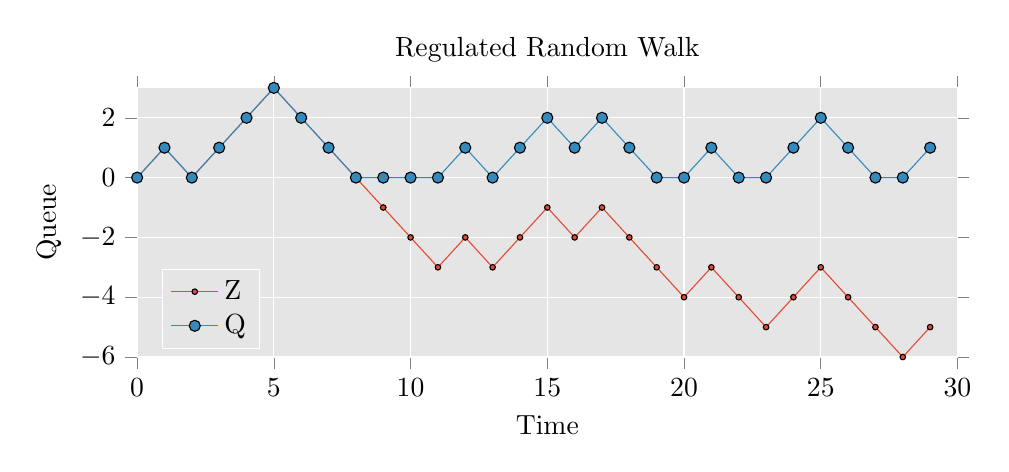
\begin{tikzpicture}

\definecolor{color0}{rgb}{0.886274509803922,0.290196078431373,0.2}
\definecolor{color1}{rgb}{0.203921568627451,0.541176470588235,0.741176470588235}

\begin{axis}[
title={Regulated Random Walk},
xlabel={Time},
ylabel={Queue},
xmin=0, xmax=30,
ymin=-6, ymax=3,
width=12cm,
height=5cm,
tick align=outside,
xmajorgrids,
x grid style={white},
ymajorgrids,
y grid style={white},
axis line style={white},
axis background/.style={fill=white!89.803921568627459!black},
legend style={at={(0.03,0.03)}, anchor=south west, draw=white, fill=white!89.803921568627459!black},
legend entries={{Z},{Q}},
legend cell align={left}
]
\addplot [color0, mark=*, mark size=1, mark options={solid,draw=black}]
table {%
0 0
1 1
2 0
3 1
4 2
5 3
6 2
7 1
8 0
9 -1
10 -2
11 -3
12 -2
13 -3
14 -2
15 -1
16 -2
17 -1
18 -2
19 -3
20 -4
21 -3
22 -4
23 -5
24 -4
25 -3
26 -4
27 -5
28 -6
29 -5
};
\addplot [color1, mark=*, mark size=2, mark options={solid,draw=black}]
table {%
0 0
1 1
2 0
3 1
4 2
5 3
6 2
7 1
8 0
9 0
10 0
11 0
12 1
13 0
14 1
15 2
16 1
17 2
18 1
19 0
20 0
21 1
22 0
23 0
24 1
25 2
26 1
27 0
28 0
29 1
};
\end{axis}

\end{tikzpicture}
\caption{The upper panel shows a graph of the random walk $Z$. An
  upward pointing triangle corresponds to an arrival, a downward
  triangle to a potential service. The lower panel shows the queueing
  process $\{Q_k\}$ as a random walk with reflection.}
\label{fig:random_bernoulli}
\end{figure}

\begin{figure}[ht]
  \centering
% see progs/reflected_random_walk.py
% This file was created by matplotlib2tikz v0.5.15.
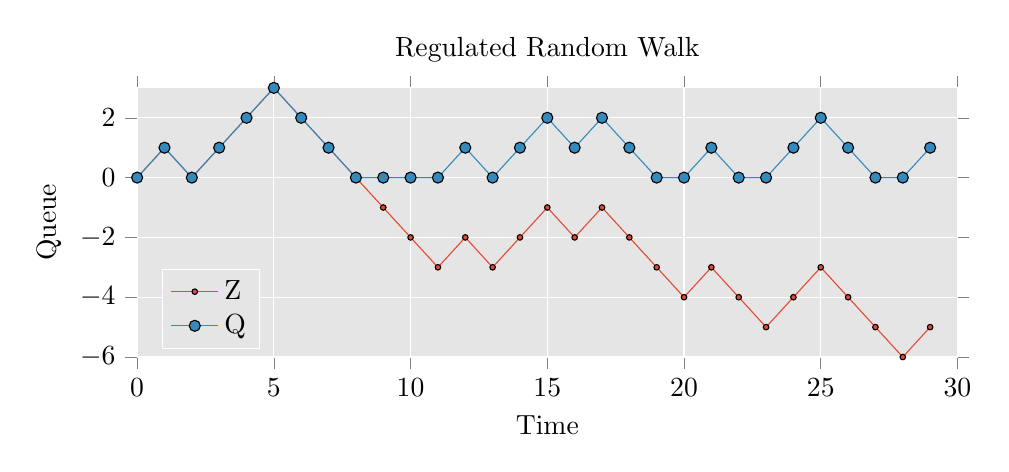
\begin{tikzpicture}

\definecolor{color0}{rgb}{0.886274509803922,0.290196078431373,0.2}
\definecolor{color1}{rgb}{0.203921568627451,0.541176470588235,0.741176470588235}

\begin{axis}[
title={Regulated Random Walk},
xlabel={Time},
ylabel={Queue},
xmin=0, xmax=30,
ymin=-6, ymax=3,
width=12cm,
height=5cm,
tick align=outside,
xmajorgrids,
x grid style={white},
ymajorgrids,
y grid style={white},
axis line style={white},
axis background/.style={fill=white!89.803921568627459!black},
legend style={at={(0.03,0.03)}, anchor=south west, draw=white, fill=white!89.803921568627459!black},
legend entries={{Z},{Q}},
legend cell align={left}
]
\addplot [color0, mark=*, mark size=1, mark options={solid,draw=black}]
table {%
0 0
1 1
2 0
3 1
4 2
5 3
6 2
7 1
8 0
9 -1
10 -2
11 -3
12 -2
13 -3
14 -2
15 -1
16 -2
17 -1
18 -2
19 -3
20 -4
21 -3
22 -4
23 -5
24 -4
25 -3
26 -4
27 -5
28 -6
29 -5
};
\addplot [color1, mark=*, mark size=2, mark options={solid,draw=black}]
table {%
0 0
1 1
2 0
3 1
4 2
5 3
6 2
7 1
8 0
9 0
10 0
11 0
12 1
13 0
14 1
15 2
16 1
17 2
18 1
19 0
20 0
21 1
22 0
23 0
24 1
25 2
26 1
27 0
28 0
29 1
};
\end{axis}

\end{tikzpicture}
\caption{Another example of a reflected random walk.}
\label{fig:random_walk}
\end{figure}


Now that we have seen that random walks can be converted into queueing
systems, we can study the transient distribution,
i.e., the distribution as a function of time, of the random walk
$\{Z_k\}$. 

\begin{exercise}  The
  free $M/M/1$ queue is a queueing process that can become
  negative. Thus, it is just the random walk
\begin{equation*}
  Z(t) = Z(0) + N_\lambda(t) - N_\mu(t), 
\end{equation*}
where the arrival process is a Poisson process $N_\lambda(t)$ and the
departure process is a Poisson process $N_\mu(t)$. Show that
\begin{equation*}
    \P{Z(t)=n}_m 
= e^{-(\lambda+\mu)t} \left(\frac\lambda\mu\right)^{(n-m)/2} \sum_{k=0}^\infty 
\frac{(t\sqrt{\lambda\mu} )^{2k+m-n}}{k!(k+m-n)!},
\end{equation*}
where $\P{\cdot}_m$ means that the random walk starts at $m$, i.e.,
$Z(0)=m$ 

As an aside, the summation includes negative factorials when
$k+m-n<0$. The tacit assumption is to take $n!\in \{\pm \infty\}$ for
$n\in \Z_-$. Another way to get around this problem is to take
$k=\max\{0, m-n\}$..
\begin{hint}
It is actually not hard, even though the expression looks
  hard. Use conditioning to see that
  $\P{Z(t)=n}_m = \P{N_\mu(t) - N_\lambda(t) = m - n}$. Then write out
  the definitions of the two Poisson distributions. Assemble
  terms. Then fiddle a bit with the terms to get
  $(t\sqrt{\lambda\mu})$. 
\end{hint}
\begin{solution}
With this we have a characterization of the queue length process as a
function of time until it hits zero for the first time. What can we
say about the distribution of $Q(t)$? With the above random walk, 
\begin{equation}\label{eq:29}
  \begin{split}
    \P{Z(t)=n}_m
&= \P{m+N_\lambda(t) - N_\mu(t) = n }  = \P{N_\lambda(t) - N_\mu(t) = n-m }  \\
&= \P{N_\mu(t) - N_\lambda(t) = m-n }  \\
&= \sum_{k=0}^\infty \P{N_\mu(t) = k - n + m\given N_\lambda(t) = k } \P{N_\lambda(t)=k}\\
&= \sum_{k=0}^\infty e^{-\mu t} \frac{(\mu t)^{k -n+m}}{(k-n +m)!} e^{-\lambda t} \frac{(\lambda t)^k}{k!} \\
&= e^{-(\lambda+\mu)t} \sum_{k=0}^\infty \frac{(\lambda t)^k(\mu t)^{k  -n + m }}{k!(k-n+m)!}.
  \end{split}
\end{equation}
We can write this a bit simpler by noting that
\begin{equation*}
  \begin{split}
  (\lambda t)^k (\mu t) ^{k + m - n} t^{k+m-n} 
&=  \lambda^k t^k\mu^{k + m - n} t^{k+m-n} \\
&= \lambda^k \mu^{k + m - n} (t\sqrt{\lambda \mu})^{2k+m-n} (\lambda\mu)^{-k + (n-m)/2} \\
&= (\lambda/\mu)^{(n-m)/2} (t\sqrt{\lambda \mu})^{2k+m-n}.
  \end{split}
\end{equation*}
With this,
\begin{equation*}
    \P{Z(t)=n} 
= e^{-(\lambda+\mu)t} \left(\frac\lambda\mu\right)^{(n-m)/2} \sum_{k=0}^\infty 
\frac{(t\sqrt{\lambda\mu} )^{2k+m-n}}{k!(k+m-n)!}.
\end{equation*}
\end{solution}
\end{exercise}


\begin{exercise}
  Can you relate the construction of $\{Q_k\}$ as a discrete-time
  random walk to a continuous-time construction of the $M/M/1$ queue?
  \begin{hint}
Consider $Z(t)=Z(0) + N_\lambda( t) -N_\mu(t)$ at the embedded
    set of epochs at which either $N_\lambda$ or $N_\mu$ changes. What
    is the probability that $N_\lambda$ fires, given that one of the
    two Poisson processes fires? Relate this to $\{a_k\}$ and
    $\{c_k\}$.
  \end{hint}
    \begin{solution}
      We use that merging two Poisson processes leads to another
      Poisson process and that a Poisson process can be split with
      Bernoulli random variables to form a thinned Poisson
      process. See one of the exercises of
      Section~\ref{sec:poisson-distribution}. 

      Consider the Poisson process $N_{\lambda+\mu}(t)$. This counting
      process has, for fixed $t$, the same distribution as
      $N_\lambda(t)+N_\mu(t)$. Let $\{A_k\}$ be the epochs at which
      the arrivals of $N_{\lambda+\mu}(t)$ occur. At $A_k$, throw a
      coin that lands heads with probability $\lambda/(\lambda+\mu)$
      and tails with probability $\mu/(\lambda+\mu)$. Set $a_k=1$ and
      $c_k=0$ if the coin lands heads, and set $a_k=0$ and $c_k=1$ if
      it turns tails. The processes
      \begin{align*}
        N_\lambda(t) &= \sum_{k=1}^\infty a_k \1{A_k \leq t},\\
        N_\mu(t) &= \sum_{k=1}^\infty c_k \1{A_k \leq t},
      \end{align*}
      are our original Poisson processes.  Observe that with this
      procedure we have established a relation between the sequences
      $\{a_k\}$ and $\{c_k\}$ and the Poisson processes $N_\lambda$ and $N_\mu$. 

      The process $Z_k = Z_{k-1}+a_k - c_k$ is a random walk in
      discrete time and its reflection results in the discrete-time
      $M/M/1$ queue. The process
      $Z(t) = Z(0) + N_\lambda(t) - N_\mu(t)$, with $N_\lambda$ and
      $N_\mu$ constructed based on the sequences $\{a_k\}$ and
      $\{c_k\}$, is the continuous-time random walk underlying the
      $M/M/1$ queue.
    \end{solution}
\end{exercise}

The solution of the above exercise shows that there is no simple
function by which we can compute the transient distribution of 
the  simple random walk $\{Z(t)\}$. Since a queueing process is typically a
more complicated object (as it is a constrained random walk), our
hopes to finding anything simple for the transient analysis of the
$M/M/1$ queue should not be too high. And the $M/M/1$ is but the
simplest queueing system; other queueing systems will be more
complicated yet.  We therefore give up the analysis of such transient
queueing systems and we henceforth contend ourselves with the analysis
of queueing systems in the limit as $t\to\infty$.  This of course
warrants two questions: what type of limit is actually meant here, and
what is the rate of convergence to this limiting situation? We address
these questions subsequently.

The \emph{long-run limiting behavior} of a queueing system is an
important topic by itself. The underlying question is what happens if
we simulate the system for a long time. For instance, does there exist
a random variable $Q$ such that $Q_k\to Q$ in some sense? The answer
to this question is in the affirmative, provided some simple stability
conditions are satisfied, see
Section~\ref{sec:rate-stability}. However, it requires a considerable
amount of mathematics to make this procedure precise. To sketch what
has to be done, first, we need to define $\{Q_k\}$ as random variables
in their own right. Note that up to now we just considered each $Q_k$
as a \emph{number}, i.e., a measurement or simulation of the queue
length time of the $k$th period. Defining $Q_k$ as a random variable
is not as simple as the definition of, for instance, the number of
arrivals $\{a_k\}$; these random variables can be safely
\emph{assumed} to be i.i.d. However, the queue lengths $\{Q_k\}$ are
certainly not i.i.d., but, as should be apparent from
Eq.~\eqref{eq:59}, they are \emph{constructed} in terms of
recursions. Next, based on these recursions, we need to show that the
sequence of distribution functions $\{G_k\}$ associated with the
random variables $\{Q_k\}$ converges to some limiting distribution
function~$G$, say. Finally, it is necessary to show that it is
possible to construct a random variable~$Q$ that has~$G$ as its
distribution function.  In this sense, then, we can say
that~$Q_k \to Q$. The random variable $Q$ is known as the
\recall{steady-state limit} of the sequence of random variables
$\{Q_k\}$, and the distribution $G$ of~$Q$ is known as the
\recall{limiting} or \emph{stationary distribution} of $\{Q_k\}$.

In these notes we sidestep all these fundamental issues, as the
details require measure theory and more advanced probability theory
than we can deal with in this course. However, it can all be made
precise. 

We illustrate the rate of convergence to the limiting situation by means of an example. Specifically, we consider the sequence of waiting times $\{W_{Q,k}\}$ to a limiting random variable
$W_Q$, where $W_{Q,k}$ is constructed according to the recursion
Eq.~(\ref{eq:56}). Suppose that $X_k\sim U\{1,2,4\}$ and
$S_k\sim U\{1,2,3\}$.  Starting with $W_{Q,0}=5$ we use
Eq.~(\ref{eq:56}) to compute the \emph{exact} distribution of
$W_{Q,k}$ for $k=1,2,\ldots, 20$, c.f., the left panel in
Figure~\ref{fig:convergence}. We see that when $k=5$, the `hump' of
$\P{W_{Q,5}=x}$ around $x=5$ is due the starting value of
$W_{Q,0}=5$. However, for $k>10$ the distribution of $W_{Q,k}$ hardly
changes, at least not visually. Apparently, the convergence of the
sequence of distributions of $W_{Q,k}$ is rather fast. In the middle
panel we show the results of a set of \emph{simulations} for
increasing simulation length, up to $N=1000$ samples. Here the
\emph{empirical distribution} for the simulation is defined as
\begin{equation*}
\P{W_Q\leq x} =   \frac 1n \sum_{k=1}^n \1{W_{Q,k} \leq x},
\end{equation*}
where $W_{Q,k}$ is obtained by simulation. As should be clear from the
figure, the simulated distribution also seems to converge quite fast to
some limiting function. Finally, in the right hand panel we compare
the densities as obtained by the exact method and simulation with
$n=1000$. Clearly, for all practical purposes, these densities can be
treated as the same.

The combination of the fast convergence to the steady-state situation
and the difficulties with the transient analysis validates, to some
extent, that most queueing theory is concerned with the analysis of
the system in \emph{stationarity}. The study of queueing systems in
stationary state will occupy us for the rest of the book.

\begin{figure}
  \centering
% see progs/waiting_time_simulation.py
% This file was created by matplotlib2tikz v0.6.18.
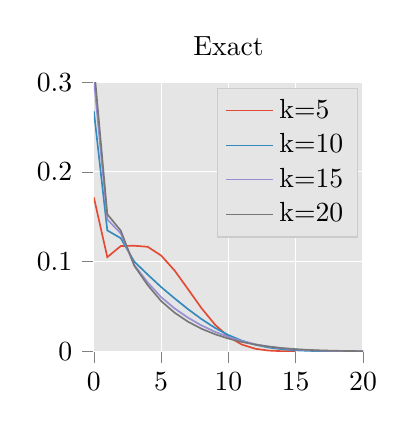
\begin{tikzpicture}

\definecolor{color0}{rgb}{0.886274509803922,0.290196078431373,0.2}
\definecolor{color1}{rgb}{0.203921568627451,0.541176470588235,0.741176470588235}
\definecolor{color2}{rgb}{0.596078431372549,0.556862745098039,0.835294117647059}

\begin{axis}[
axis background/.style={fill=white!89.80392156862746!black},
axis line style={white},
height=5cm,
legend cell align={left},
legend entries={{k=5},{k=10},{k=15},{k=20}},
legend style={draw=white!80.0!black, fill=white!89.80392156862746!black},
tick align=outside,
tick pos=left,
title={Exact},
width=5cm,
x grid style={white},
xmajorgrids,
xmin=0, xmax=20,
y grid style={white},
ymajorgrids,
ymin=0, ymax=0.3
]
\addlegendimage{no markers, color0}
\addlegendimage{no markers, color1}
\addlegendimage{no markers, color2}
\addlegendimage{no markers, white!46.666666666666664!black}
\addplot [semithick, color0]
table [row sep=\\]{%
0	0.171637114938441 \\
1	0.104963674236651 \\
2	0.117394028688039 \\
3	0.117715795356399 \\
4	0.116547274297617 \\
5	0.10680959880777 \\
6	0.0901116022286576 \\
7	0.0692645091364799 \\
8	0.048095649375942 \\
9	0.0298057545428373 \\
10	0.0162068790326678 \\
11	0.00753611407475148 \\
12	0.00287896492743315 \\
13	0.000846754390421514 \\
14	0.000169350878084303 \\
15	1.69350878084303e-05 \\
};
\addplot [semithick, color1]
table [row sep=\\]{%
0	0.267670098481664 \\
1	0.134811729932366 \\
2	0.126115559618164 \\
3	0.100031570893792 \\
4	0.0856111019982735 \\
5	0.0716606125484384 \\
6	0.0590583363688737 \\
7	0.0470211200764174 \\
8	0.0359432992083069 \\
9	0.0262065053330494 \\
10	0.0181445546165273 \\
11	0.0118798282991401 \\
12	0.0073250777973754 \\
13	0.00423423971833927 \\
14	0.00228253344190638 \\
15	0.0011402678063088 \\
16	0.000523855446719374 \\
17	0.000219223477018188 \\
18	8.25631776709328e-05 \\
19	2.75497389435522e-05 \\
20	7.97697729519009e-06 \\
21	1.94735298174807e-06 \\
22	3.84308246766187e-07 \\
23	5.73594398158488e-08 \\
24	5.73594398158488e-09 \\
25	2.86797199079244e-10 \\
};
\addplot [semithick, color2]
table [row sep=\\]{%
0	0.30317953657453 \\
1	0.14699251783874 \\
2	0.131469895956502 \\
3	0.0963326761914749 \\
4	0.076869973873194 \\
5	0.0604280411223663 \\
6	0.04784522712146 \\
7	0.0374709958541702 \\
8	0.0289083894170772 \\
9	0.0218171288010453 \\
10	0.0160366591920489 \\
11	0.0114368309310598 \\
12	0.00789001335365536 \\
13	0.00525183269083643 \\
14	0.00336515460534012 \\
15	0.0020710966262499 \\
16	0.00122159902225598 \\
17	0.00068892069543721 \\
18	0.000370520942164379 \\
19	0.000189507686033138 \\
20	9.18799257332931e-05 \\
21	4.20732116476868e-05 \\
22	1.8119623555642e-05 \\
23	7.30325357242076e-06 \\
24	2.73902579612197e-06 \\
25	9.49296970741557e-07 \\
26	3.01535089774823e-07 \\
27	8.68973074166946e-08 \\
28	2.24352547533544e-08 \\
29	5.10658224714927e-09 \\
30	1.00330207473452e-09 \\
31	1.65305808238278e-10 \\
32	2.1904780230781e-11 \\
33	2.18562108732849e-12 \\
34	1.45708072488566e-13 \\
35	4.85693574961886e-15 \\
};
\addplot [semithick, white!46.666666666666664!black]
table [row sep=\\]{%
0	0.319144828865997 \\
1	0.152832481719423 \\
2	0.134555843047554 \\
3	0.0955843772093346 \\
4	0.0738400658782454 \\
5	0.0560416473000174 \\
6	0.0430735344931855 \\
7	0.0330094400597946 \\
8	0.0252025073900232 \\
9	0.0190619218519665 \\
10	0.0142314981096182 \\
11	0.0104502968908312 \\
12	0.00752571097051776 \\
13	0.00530189974927228 \\
14	0.0036465388505557 \\
15	0.00244409730130202 \\
16	0.00159388825481048 \\
17	0.00100987966393171 \\
18	0.000620806320781876 \\
19	0.000369768373140325 \\
20	0.000213105770501226 \\
21	0.000118668173969863 \\
22	6.37517889450218e-05 \\
23	3.29887723679431e-05 \\
24	1.64131133653723e-05 \\
25	7.83660826357756e-06 \\
26	3.58303411938414e-06 \\
27	1.56505220483645e-06 \\
28	6.51341807039512e-07 \\
29	2.57510039633041e-07 \\
30	9.63864754135865e-08 \\
31	3.40252853261261e-08 \\
32	1.12779804213856e-08 \\
33	3.49207550281559e-09 \\
34	1.00407169477642e-09 \\
35	2.66202450453925e-10 \\
36	6.45301076626973e-11 \\
37	1.41567960213762e-11 \\
38	2.77528281343393e-12 \\
39	4.78404346590005e-13 \\
40	7.10027762243559e-14 \\
41	8.8158372477798e-15 \\
42	8.78458124708791e-16 \\
43	6.58021067197597e-17 \\
44	3.29010533598798e-18 \\
45	8.22526333996996e-20 \\
};
\end{axis}

\end{tikzpicture}
% This file was created by matplotlib2tikz v0.6.18.
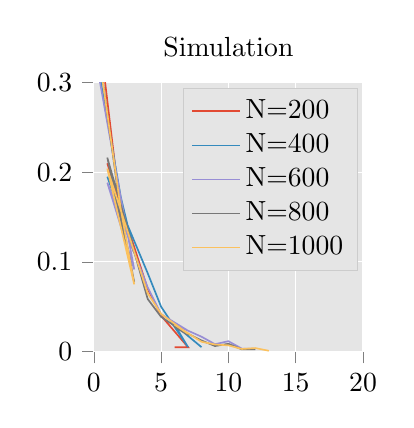
\begin{tikzpicture}

\definecolor{color0}{rgb}{0.886274509803922,0.290196078431373,0.2}
\definecolor{color1}{rgb}{0.203921568627451,0.541176470588235,0.741176470588235}
\definecolor{color2}{rgb}{0.596078431372549,0.556862745098039,0.835294117647059}
\definecolor{color3}{rgb}{0.984313725490196,0.756862745098039,0.368627450980392}

\begin{axis}[
axis background/.style={fill=white!89.80392156862746!black},
axis line style={white},
height=5cm,
legend cell align={left},
legend entries={{N=200},{N=400},{N=600},{N=800},{N=1000}},
legend style={draw=white!80.0!black, fill=white!89.80392156862746!black},
tick align=outside,
tick pos=left,
title={Simulation},
width=5cm,
x grid style={white},
xmajorgrids,
xmin=0, xmax=20,
y grid style={white},
ymajorgrids,
ymin=0, ymax=0.3
]
\addlegendimage{no markers, color0}
\addlegendimage{no markers, color1}
\addlegendimage{no markers, color2}
\addlegendimage{no markers, white!46.666666666666664!black}
\addlegendimage{no markers, color3}
\addplot [semithick, color0]
table [row sep=\\]{%
0	0.405 \\
2	0.155 \\
3	0.11 \\
1	0.21 \\
4	0.07 \\
5	0.04 \\
7	0.005 \\
6	0.005 \\
};
\addplot [semithick, color1]
table [row sep=\\]{%
0	0.345 \\
2	0.1725 \\
3	0.11 \\
1	0.195 \\
4	0.0875 \\
5	0.05 \\
7	0.005 \\
6	0.03 \\
8	0.005 \\
};
\addplot [semithick, color2]
table [row sep=\\]{%
0	0.338333333333333 \\
2	0.171666666666667 \\
3	0.0916666666666667 \\
1	0.188333333333333 \\
4	0.0716666666666667 \\
5	0.0416666666666667 \\
7	0.0233333333333333 \\
6	0.03 \\
8	0.0166666666666667 \\
9	0.00833333333333333 \\
10	0.0116666666666667 \\
11	0.00333333333333333 \\
12	0.00333333333333333 \\
};
\addplot [semithick, white!46.666666666666664!black]
table [row sep=\\]{%
0	0.375 \\
2	0.155 \\
3	0.0775 \\
1	0.21625 \\
4	0.05875 \\
5	0.03875 \\
7	0.01875 \\
6	0.0275 \\
8	0.0125 \\
9	0.00625 \\
10	0.00875 \\
11	0.0025 \\
12	0.0025 \\
};
\addplot [semithick, color3]
table [row sep=\\]{%
0	0.371 \\
2	0.159 \\
3	0.075 \\
1	0.204 \\
4	0.065 \\
5	0.042 \\
7	0.02 \\
6	0.03 \\
8	0.011 \\
9	0.008 \\
10	0.007 \\
11	0.003 \\
12	0.004 \\
13	0.001 \\
};
\end{axis}

\end{tikzpicture}
% This file was created by matplotlib2tikz v0.6.18.
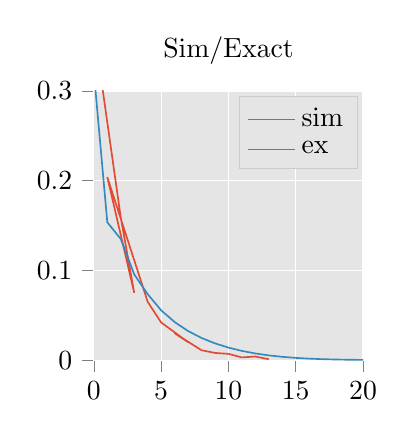
\begin{tikzpicture}

\definecolor{color0}{rgb}{0.886274509803922,0.290196078431373,0.2}
\definecolor{color1}{rgb}{0.203921568627451,0.541176470588235,0.741176470588235}

\begin{axis}[
axis background/.style={fill=white!89.80392156862746!black},
axis line style={white},
height=5cm,
legend cell align={left},
legend entries={{sim},{ex}},
legend style={draw=white!80.0!black, fill=white!89.80392156862746!black},
tick align=outside,
tick pos=left,
title={Sim/Exact},
width=5cm,
x grid style={white},
xmajorgrids,
xmin=0, xmax=20,
y grid style={white},
ymajorgrids,
ymin=0, ymax=0.3
]
\addlegendimage{no markers, color0}
\addlegendimage{no markers, color1}
\addplot [semithick, color0]
table [row sep=\\]{%
0	0.371 \\
2	0.159 \\
3	0.075 \\
1	0.204 \\
4	0.065 \\
5	0.042 \\
7	0.02 \\
6	0.03 \\
8	0.011 \\
9	0.008 \\
10	0.007 \\
11	0.003 \\
12	0.004 \\
13	0.001 \\
};
\addplot [semithick, color1]
table [row sep=\\]{%
0	0.321210551486458 \\
1	0.153610083372614 \\
2	0.134996882888543 \\
3	0.0955453595314327 \\
4	0.0735078887084144 \\
5	0.0555229800002277 \\
6	0.04248374875847 \\
7	0.0324340034608454 \\
8	0.0247003408996893 \\
9	0.0186641447360399 \\
10	0.0139463946460717 \\
11	0.0102694858215254 \\
12	0.00743088327585761 \\
13	0.00527073128751502 \\
14	0.00365717229905777 \\
15	0.00247795939414692 \\
16	0.00163698266495181 \\
17	0.00105290221377686 \\
18	0.000658507879443266 \\
19	0.000399962283965939 \\
20	0.000235625724146408 \\
21	0.000134469080633985 \\
22	7.42414402995369e-05 \\
23	3.9599462856611e-05 \\
24	2.03752070292254e-05 \\
25	1.00967419862763e-05 \\
26	4.81015048751568e-06 \\
27	2.19881789346049e-06 \\
28	9.62361553682428e-07 \\
29	4.0231467941736e-07 \\
30	1.60217273745469e-07 \\
31	6.05984076836477e-08 \\
32	2.1694159117719e-08 \\
33	7.32269701357755e-09 \\
34	2.32015184679573e-09 \\
35	6.86512898604053e-10 \\
36	1.88567121134715e-10 \\
37	4.77418033968616e-11 \\
38	1.10478769598855e-11 \\
39	2.31287446547169e-12 \\
40	4.32519221532182e-13 \\
41	7.10963979995277e-14 \\
42	1.0058482615638e-14 \\
43	1.19011335266025e-15 \\
44	1.12978561565232e-16 \\
45	8.06075807317056e-18 \\
46	3.83845622531931e-19 \\
47	9.13918148885551e-21 \\
};
\end{axis}

\end{tikzpicture}
%  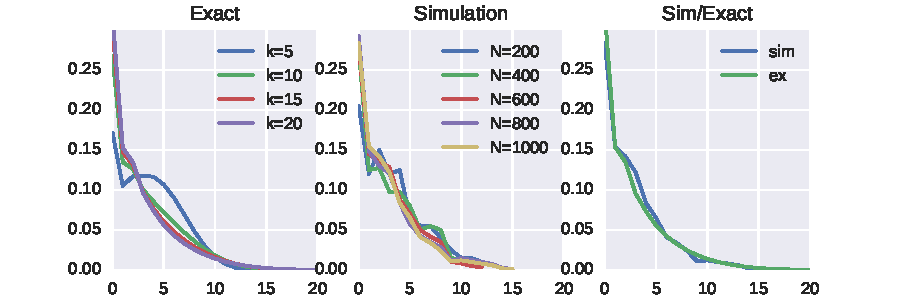
\includegraphics{progs/gg1convergence}
  \caption{The density of $W_{Q,k}$ for $k=5, 10, 15, 20$ computed by
    an exact method as compared the density obtained by simulation of
    different run lengths $N=200, 400, \ldots 1000$. The right panel
    compares the exact density of $W_{Q,20}$ to the density obtained by simulation
    for $N=1000$.}
\label{fig:convergence}
\end{figure}




\begin{exercise}
  Suppose that $X_k\in\{1,3\}$ such that $\P{X_k=1}=\P{X_k=3}$ and
  $S_k\in\{1,2\}$ with $\P{S_k=1}=\P{S_k=2}$. Write a computer program
  to see how fast the distributions of $W_{Q,k}$ converge to a limiting distribution function.
  \begin{solution}
Here is an example with python. In R it must be equally simple.
I compute the 
difference, i.e., the Kolmogorov-Smirnov statistic, between
the distributions of $W_k$ and $W_{k+1}$, 
\begin{equation*}
  \max_x\{ |\P{W_{Q,k}\leq x} - \P{W_{Q,k-1}\leq x}|\},
\end{equation*}
for $x$ in the support of $W_{Q,k}$. 

\begin{pyconsole}
  
from lea import Lea

S = Lea.fromVals(1,  2)
X = Lea.fromVals(1,  3)
U = S-X

W = Lea.fromVals(3)
for k in range(1, 10):
    W_new = Lea.fastMax(W + U, 0)
    m = max(abs(W_new.cdf(x)-W.cdf(x))  for x in range(W_new.support()[-1]))
    print(k, m) 
    W = W_new

\end{pyconsole}

So, after some 10 customers, the distribution hardly changes anymore. 

  \end{solution}
  \end{exercise}

\begin{exercise}
  Validate the results of  Figure~\ref{fig:convergence} with simulation.
  \begin{solution}
    You can study \texttt{waiting\_time\_simulation.py} at
    \href{https://github.com/ndvanforeest/queueing_book/tree/master/progs}{github}
    if you like, but skipping it is OK. Trying to make the graph in
    your favorite programming language is fun.
\end{solution}
\end{exercise}

\Closesolutionfile{hint}
\Closesolutionfile{ans}
\subsection*{Hints}
\input{hint}
\subsection*{Solutions}
\input{ans}
\clearpage

%%% Local Variables:
%%% mode: latex
%%% TeX-master: "../book"
%%% End:

%\section{Rate Stability and Utilization}
\label{sec:rate-stability}

\subsection*{Theory and Exercises}

\Opensolutionfile{hint}
\Opensolutionfile{ans}

In the analysis of any queueing process the first step should be to
check the relations between the arrival, service and departure
rates. The concept of rate is crucial because it captures our
intuition that when, on the long run, jobs arrive faster than they can
leave, the system must `explode'. Thus, the first performance measures
we need to estimate when analyzing a queueing system are the arrival
and departure rate, and then we need to check that the arrival rate is
smaller than the departure rate. In particular, the load, defined as
the ratio of the arrival rate and service rate is of importance. In
this section we define and relate these concepts.  As a reminder, we
keep the discussion in these notes mostly at an intuitive level, and
refer to \cite{el-taha98:_sampl_path_analy_queuein_system} for proofs
and further background.


We first formalize the \emph{arrival rate} and \emph{departure rate}
in terms of the \emph{counting processes} $\{A(t)\}$ and $\{D(t)\}$.
The \recall{arrival rate} is the long-run average number of jobs that
arrive per unit time, i.e.,
\begin{equation}
  \label{eq:3}
  \lambda = \lim_{t\to\infty} \frac{A(t)}t.
\end{equation}
We remark in passing that this limit does not necessarily exist if
$A(t)$ is some pathological function. If, however, the interarrival
times $\{X_k\}$ are the basic data, and $\{X_k\}$ are i.i.d.  and
distributed as a generic random variable $X$ with finite mean $\E{X}$,
we can construct $\{A_k\}$ and $\{A(t)\}$ as described in
Section~\ref{sec:constr-gg1-queu}; the strong law of large numbers
guarantees that the above limit exists.

\begin{exercise}
  Can you make an arrival process such that $A(t)/t$ does not have a
  limit?  
  \begin{hint}
As a start, the function $\sin(t)$ has not a limit as
    $t\to\infty$. However, the time-average $\sin(t)/t \to 0$.  Now
    you need to make some function whose time-average does not
    converge, hence it should grow fast, or fluctuate wilder and
    wilder.
  \end{hint}
  \begin{solution}
 If $N(t) = 3 t^2$, then clearly $N(t)/t = 3t$. This does not
    converge to a limit. 

  Another example, let the arrival rate $\lambda(t)$ be given as
    follows:
    \begin{equation*}
      \lambda(t) = 
    \begin{cases}
      1 & \text{if } 2^{2k} \leq t < 2^{2k+1} \\
      0 & \text{if } 2^{2k+1} \leq t < 2^{2(k+1)},
    \end{cases}
    \end{equation*}
    for $k=0,1,2,\ldots$. Let $N(t) = \lambda(t) t$. Then $A(t)/t$
    does not have limit. Of course, these examples are quite
    pathological, and are not representable for `real life cases'
    (Although this is also quite vague. What, then, is a real life
    case?)

For the mathematically interested, we seek a
    function for which its Ces\`aro limit does not exist.
  \end{solution}
\end{exercise}



Observe that at time $t=A_n$, precisely $n$ arrivals occurred. Thus,
by applying the definition of $A(t)$ at the epochs $A_n$, we see that
$A(A_n) = n$. Thus,
\begin{equation*}
  \frac{1}n\sum_{k=1}^n X_k = \frac{A_n}n = \frac{A_n}{A(A_n)}. 
\end{equation*}
But since $A_n\to\infty$ if $n\to\infty$, it follows from
Eq.~(\ref{eq:3}) that the average interarrival time between two
consecutive jobs is
\begin{equation}\label{eq:54}
  \E X = \lim_{n\to\infty}  \frac{1}n\sum_{k=1}^n X_k = \lim_{n\to \infty} \frac{A_n}{A(A_n)} = \lim_{t\to\infty} \frac t{A(t)} = \frac 1 \lambda,
\end{equation}
where we take $t=A_n$ in the limit for $t\to\infty$.  In words, the
above states that the arrival rate $\lambda$ is the inverse of the
expected interarrival time.

\begin{exercise}
    Eq. (\ref{eq:54}) we replaced the limit with respect to $n$ by a
    limit with respect to $t$.  Use
    the notation $A_{A(t)}$ to show that  this is allowed.
  Show next that the function $t\to A(t)$ as defined by Eqs.~(\ref{eq:2})
  is right-continuous. (This exercise is meant to provide some insight into what needs
  to be done to put everything on solid ground.  If you are not
  interested in the maths, you can skip the problem.)
    \begin{hint}
 Use that $A_{A(t)} \leq t < A_{A(t)+1}$. Divide by $A(t)$
      and take suitable limits. BTW, such type of proof is used quite
      often to show that the existence of one limit implies, and is
      implied by, the existence of another type of limit.  
    \end{hint}
 \begin{solution}
 Observing that $A_{A(t)}$ is the arrival time of the last job
    before time $t$ and that $A_{A(t)+1}$ is the arrival time of the
    first job after time $t$: 
  \begin{equation*}
    A_{A(t)}  \leq t  < A_{A(t)+1} \Leftrightarrow 
    \frac{A_{A(t)}} {A(t)}  \leq \frac{t}{A(t)}  <\frac{A_{A(t)+1}}{A(t)} = \frac{A_{A(t)+1}}{A(t)+1}\frac{A(t)+1}{A(t)}
  \end{equation*}
  Now $A(t)$ is a counting process such that $A(t)\to\infty$ as
  $t\to\infty$. Therefore, $\lim_t A_{A(t)}/A(t) = \lim_n
  A_n/n$.
  Moreover, it is evident that
  $\lim_t A_{A(t)+1}/(A(t)+1) = \lim_t A_{A(t)}/A(t)$, and that
  $(A(t)+1)/A(t)\to 1$ as $t\to\infty$. Thus it follows from the above
  inequalities that $\lim_n A_n/n = \lim_t t/A(t)$.
     

  Hopefully this problem, and its solution, clarifies that even such
  small details require attention. If we want to make some progress
  with respect to developing some queueing theory, we have to skip
  most of the proofs and mathematical problems; we simply don't have
  enough time in this course  to be concerned with all theorems
  and proofs.


  For the right-continuity of $A(t)$, define $f(t) = 1\{A_1 \leq
  t\}$.
  Observe first that $f(t)$ is increasing, and $f(t)\in\{0,1\}$. Thus,
  if $f(t)=1$ then $f(u)=1$ for all $u\geq t$, and if $f(t)=0$ then
  $f(u) = 0$ for all $u\leq t$.

    You may skip the rest of the prove below, but the above is
    essential to memorize; make a plot of $f(t)$, in particular the
    behavior around $A_1$ is important.

    We need to prove, for right-continuity, that $f(u)\to f(t) $ as
    $u\downarrow t$. When $f(t)=1$, $f(u)=1$ for any $u>1$, by the
    definition of $f(x)$. When $f(t)=0$ we have to do a bit more
    work. Formally, we have to prove that, for fixed $t$ and for all
    $\epsilon > 0$, there is a $\delta>0$ such that
    $u\in(t, t+\delta) \Rightarrow |f(u) -f(t)| < \epsilon$. (Note the
    differences with the regular definition of continuity.) Since, by
    assumption, $t$ is such that $f(t)=0$, and $f\in\{0,1\}$ we need
    to show that $f(u)=0$ for $u\in(t, t+\delta)$. Now, clearly, if
    $f(t)=0$ only if $t < A_1$.  But, then for any $u\in(t, A_1)$, we
    have that $f(u) = 0$. Thus, taking $\delta = A_1 - t$ suffices.

    The next step is to observe that $A(t)$ is a sum of
    right-continuous functions whose steps do not overlap since by
    assumption $0<A_1 < A_2 < \cdots$. As $A$ is (almost surely)
    finite sum of bounded, increasing and right-continuous functions,
    it is also right-continuous.

    If you like, you can try to prove this last step too. 


    % For finite sums it is simple. Suppose that $f$ and $g$ are
    % right-continuous, then
    % \begin{equation*}
    %   |f(u) + g(u) - f(t) - g(t)| \leq |f(u)-f(t)|+|g(u)-g(t)|.
    % \end{equation*}
    % Since both terms at the right hand side can be made arbitrarily
    % small, the left hand side can also be made as small as we
    % like. With this we can see that the function
    % $F_N(t) = \sum_{n=1}^N f_n(x)$ is right-continuous if all $f_n$
    % are right-continuous, and also that $F_{N+1} = F_N + f_{N+1}$ is
    % right-continuous. As this applies for all $N$, it follows from
    % induction that $\lim_N F_N$ is right-continous, provided this
    % limit exists. When $f_n$ are all increasing, which is the case for
    % our situation by taking $f_n(t) = 1\{A_n \leq t\}$, then this
    % limit certainly exists.
 \end{solution}
\end{exercise}

The development of the departure times $\{D_k\}$ is entirely analogous
to that of the arrival times; we leave it to the reader to provide the
details. As a result we can define the \recall{departure rate} as
\begin{equation}\label{eq:28}
  \lim_{t\to\infty} \frac{D(t)}t = \gamma
\end{equation}


\begin{exercise}
  Define the departure time $D_{k}$ of the $k$th job in terms of
  $\{D(t)\}$. 
  \begin{hint}
Use the analogy with Eq.~\eqref{eq:27}.
  \end{hint}
\begin{solution}
  \begin{equation*}
 D_{k} = \inf\{t; D(t) \geq k\}.
  \end{equation*}
\end{solution}
\end{exercise}

Assume now that there is a single server. Let $S_k$ be the required
service time of the $k$th job to be served, and define
\begin{equation*}
U_n = \sum_{k=1}^n S_k
\end{equation*}
as the total service time required by the first $n$ jobs. With this,
let 
\begin{equation*}
  U(t) = \sup\{n: U_n \leq t\}.
\end{equation*}
and  define the \recall{service } or \emph{processing rate} as
\begin{equation*}
  \mu = \lim_{t\to\infty} \frac{U(t)}t.
\end{equation*}
In the same way as we derived that $\E X= 1/\lambda$, we obtain for
the expected (or average) amount of service required by an individual
job
\begin{equation*}
  \E S = \lim_{n\to\infty} \frac 1 n \sum_{k=1}^n S_k = \lim_{n\to\infty} \frac{U_n}{n} = \lim_{n\to\infty} \frac{U_n}{U(U_n)} = \lim_{t\to\infty} \frac t{U(t)} = \frac 1 \mu.
\end{equation*}

Now observe that, if the system is empty at time $0$, it must be that
at any time the number of departures must be smaller than the number
of arrivals, i.e., $D(t) \leq A(t)$ for all $t$. Therefore,
\begin{equation}\label{eq:26}
\gamma :=   \lim_t \frac{D(t)}t \leq \lim_t \frac{A(t)}t = \lambda.
\end{equation}
We call a system \recall{(rate) stable} if
\begin{equation*}
  \lambda = \gamma,
\end{equation*}
in other words, the system is stable if, on the long run, jobs leave
the system just as fast as they arrive. Of course, if
$\lambda > \gamma$, the system length process $L(t) \to \infty$ as
$t\to \infty$.

It is also evident that jobs cannot depart faster than they can be
served, hence, $D(t) \leq U(t)$ for all~$t$. Combining this with the
fact that $\gamma \leq \lambda$, we get
\begin{equation*}
  \gamma \leq \min\{\lambda, \mu\}.
\end{equation*}
When $\mu \geq \lambda$ the above inequality reduces to
$\gamma = \lambda$ for rate-stable systems. (It is interesting to
prove this.) As it turns out, when $\mu = \lambda$ and the variance of
the service times $\V{S} > 0$ or $\V{X} >0$ then $\lim_t L(t)/t$
does not necessarily exist. For this reason we henceforth require that
$\mu > \lambda$.



\begin{exercise} 
Define the random variables $\{\tilde X_k,k=1,\ldots\}$ as $\tilde X_k = S_{k-1}-X_k$.
  For stability of the queueing process it is essential that
  $\tilde X_k$ has negative expectation, i.e.,
  $\E{\tilde X_k} = \E{S_{k-1}-X_k} < 0$.  What is the conceptual
  meaning of this inequality?
  \begin{solution}
 That the average time customers spend in service is smaller
      than the average time between the arrival of two subsequent
      jobs. 
  \end{solution}
\end{exercise}

\begin{exercise} 
Define $\tilde X_k = S_{k-1}-X_k$.
 Show that $\E{\tilde X_k} <0$ implies that $\lambda<\mu$. 
 \begin{hint}
Remember that $\{X_k\}$ and $\{S_k\}$ are sequences of i.i.d. random variables. What are the implications for the expectations?
 \end{hint}
  \begin{solution}
  $0> \E{\tilde X_k} = \E {S_{k-1}-X_k} =  \E{ S_{k-1}}- \E {X_k} = \E S - \E X$, where we use the fact that the $\{S_k\}$ and $\{X_k\}$ are i.i.d. sequences. Hence, 
  \begin{equation*}
    \E X > \E S \iff \frac 1{\E S} > \frac1{\E X} \iff \mu > \lambda.
  \end{equation*}

  \end{solution}
\end{exercise}


\begin{exercise}
  Show that $\E{S}/\E{X}$ is the fraction of time the server is busy.
  \begin{hint}
Let $T_1>A_1$ be the first time after the arrival of job 1
    that arrives at an empty system. (Observe that job 1 also arrives
    at an empty system.)  Suppose, for ease of writing, that this job
    is the $n+1$th job, so that up to time $T_1$ the number of
    arrivals is $n$. Since the first job arrived at time $A_1=X_1$,
    the first $n$ jobs arrived during $[X_1, T_1)$. The total amount
    of service that arrived during this period is $\sum_{i=1}^n S_i$.
    What is the fraction of time the server has been busy in this
    cycle?
  \end{hint}
  \begin{solution}
 The
    fraction of time that the server has been busy during $[X_1, T_1)$
    is
        \begin{equation*}
\frac{\sum_{i=1}^n S_i}{T_1-X_1} 
=          \frac{\sum_{i=1}^n S_i}{\sum_{i=1}^{n+1}X_i -X_1} 
=          \frac{\sum_{i=1}^n S_i}{\sum_{i=2}^{n+1}X_i} 
        \end{equation*}
        Now use the assumption that the $\{X_i\}$ and $\{S_i\}$ are
        sequences of i.i.d. random variables distributed as the
        generic random variables $X$ and $S$, respectively. Then by
        taking expectations the above becomes
        \begin{equation*}
\frac{\E{\sum_{i=1}^n S_i}}{\E{\sum_{i=2}^{n+1}X_i}} 
= \frac{n \E S }{n \E X} =
 \frac{ \E S }{ \E X}.
        \end{equation*}

        These busy cycles occur over and over again. Thus, the
        long-run average fraction of time the server is busy must also
        be $\E S/\E X$. (For the die-hards, there is a subtle point
        here: the arrival epochs of the $G/G/1$ queue are not real
        renewal moments, hence the epochs at which the busy times
        start also do not form a sequence of renewal times. But then
        it is not true, in general, that the busy times $\{B_i\}$ have
        the same distribution, neither do the idles times
        $\{I_n\}$. Showing that in the limit all is OK requires a
        substantial amount of mathematics. The above claim is still
        true however.)
  \end{solution}
\end{exercise}

\begin{exercise}
 Show that $\E{X - S}/\E{X}$ is the fraction of time
  the server is idle.
  \begin{solution}
    Since the fraction of idle time is $1$ minus the fraction of busy
    time, it follows that $1-\E S/ \E X = (\E X - \E S)/\E X$ is the
    idle time fraction.
  \end{solution}
\end{exercise}

The concept of \recall{load} or \emph{utilization}, denoted by the
symbol $\rho$, is fundamental. One way to define this is  as the limiting
fraction of time the server is busy, i.e.,
\begin{equation*}
  \rho = \lim_{t\to\infty} \frac 1 t \int_0^t \1{L(s)>0} \d s.
\end{equation*}
Interestingly, we can express this in terms of the arrival rate
$\lambda$ and service rate $\mu$. Observe that
\begin{equation*}
  \sum_{k=1}^{A(t)} S_k \geq \int_0^t \1{L(s)>0} \d s \geq   \sum_{k=1}^{D(t)} S_k,
\end{equation*}
since $t$ can lie half way a service interval and $A(t) \geq D(t)$. As
$A(t)\to \infty$ as $t\to\infty$,
\begin{equation*}
  \lim_{t\to\infty} \frac 1 t\sum_{k=1}^{A(t)} S_k = 
  \lim_{t\to\infty} \frac{A(t)}t \frac{1}{A(t)} \sum_{k=1}^{A(t)} S_k = 
  \lim_{t\to\infty} \frac{A(t)}t \cdot \lim_{t\to\infty}\frac{1}{A(t)} \sum_{k=1}^{A(t)} S_k = \lambda \E S.
\end{equation*}
Applying similar limits to the other inequality gives
\begin{equation*}
\lambda \E S \geq \rho \geq \gamma \E S.
\end{equation*}
Hence, if $\gamma=\lambda$, $\rho = \lambda \E S$.  

From the identies $\lambda^{-1} = \E X$ and $\mu^{-1} = \E S$, we get
a further set of relations:
\begin{equation*}
  \rho = \lambda \E S = \frac{\lambda}{\mu} = \frac{\E S}{\E X}.
\end{equation*}
Thus, the load has also the interpretation as the rate at which jobs
arrive times the average amount of work per job.  Finally,
recall that for a system to be rate-stable, it is necessary that
$\mu> \lambda$, implying in turn that $\rho < 1$. The relation
$\rho=\E S/ \E X < 1$ then tells us that the average time it takes to
serve a job must be less than the average time between two consecutive
arrivals, i.e., $\E S < \E X$.


\begin{exercise}
  Consider a queueing system with $c$ identical servers (identical in
  the sense that each server has the same production rate $\mu$). What would be a reasonable stability criterion for this system? 
  \begin{hint}
What is the rate in, and what is the service capacity?
  \end{hint}
  \begin{solution}
    The criterion is that $c$ must be such that $\lambda <
    c\mu$.
    (Thus, we interpret the number of servers as a \emph{control},
    i.e., a `thing' we can change, while we assume that $\lambda$ and
    $\mu$ cannot be easily changed.) To see this, we can take two
  different points of view.  Imagine that the $c$ servers are replaced
  by one server that works $c$ times as fast. The service capacity of
  these two systems (i.e., the system with $c$ servers and the system
  with one fast server) is the same, i.e., $c\mu$, where $\mu$ is the
  rate of one server. For the system with the fast server the load is
  defined as $\rho =\lambda/c\mu$, and for stability we require
  $\rho<1$.  Another way to see it is to assume that the stream of
  jobs is split into $c$ smaller streams, each with arrival rate
  $\lambda/c$.  In this case, applying the condition that
  $(\lambda/c )/\mu<1$ per server leads to the same condition that
  $\lambda/(c\mu) < 1$.
  \end{solution}
\end{exercise}

\begin{exercise}
  Check with simulation that when $\lambda > \mu$ the queue length
  grows roughly linearly with slope $\lambda - \mu$.  Thus, if
  $\rho>1$, `we are in trouble'.
  \begin{solution}
    See my website. 
  \end{solution}
\end{exercise}


\begin{exercise}\label{ex:11}
  If $\E{B}$ is the expected busy time and $\E{I}$ is the expected idle
  time, show that $\E{B} = \E{I} \rho/(1-\rho) $
 is the fraction of time the  server is busy.
\begin{solution}
  Consider a busy cycle, that is, a cycle that starts with the first
  job that sees an empty system at upon arrival up to the time another
  job sees an empty system upon arrival. In such one cycle, the server
  is busy for an expected duration $\E{B}$. The total expected length
  of the cycle is $\E{B} + \E{I}$, since after the last job of the cycle
  left, the expected time until the next job is $\E{I}$.

  Since $\rho$ is utilization of the server,
  \begin{equation*}
\rho = \frac{\E B}{\E B + \E I}.
  \end{equation*}
  With a bit of algebra the result follows.
\end{solution}
\end{exercise}

\begin{exercise}
  Consider a paint factory which contains a paint mixing machine that
  serves two classes of jobs, A and B. The processing times of jobs of
  types A and B are constant and require $t_A$ and $t_B$ hours. The
  job arrival rate is $\lambda_A$ for type A and $\lambda_B$ for type
  $B$ jobs. It takes a setup time of $S_s$ hours to clean the mixing
  station when changing from paint type A to type B, and there is no
  time required to change from type B to A.

  To keep the system (rate) stable, it is necessary to produce the
  jobs in batches, for otherwise the server, i.e., the mixing machine,
  spends a too large fraction of time on setups, so that
  $\mu < \lambda$. Thus, it is necessary to identify minimal batch
  sizes to ensure that $\mu > \lambda$.  Motivate that the following linear
  program  can be used to determine the minimal batch sizes:
\begin{equation*}
  \text{minimize }  T
\end{equation*}
such that $ T=  k_A t_A + S + k_B t_B$, $\lambda_A T < k_A$ and $\lambda_B T < k_B$.
\begin{hint}
Here are some questions to help you interpret this formulation.
\begin{enumerate}
\item   What are the decision variables for this problem? In other words, what are the `things' we can control/change?
\item What are the interpretations of $k_A t_A$, and $S+k_B t_B$?
\item What is the meaning of the first constraint?  Realize that $T$
  represents one production cycle. After the completion of one such
  cycle, we start another cycle. Hence, the start of every cycle can
  be seen as a restart of the entire system.
\item   What is the meaning of the other two constraints?
\item Why do we minimize the cycle time $T$?
\item Solve for $k_A$ and $k_B$ in terms of $S$,  $\lambda_A, \lambda_B$ and $t_A, t_B$. 
\item Generalize this to $m$ job classes and such that the cleaning
  time between jobs of class $i$ and $j$ is given by $S_{ij}$. (Thus,
  the setup times are sequence dependent.) 
\end{enumerate}
\end{hint}

  \begin{solution}
    Realize that the machine works in cycles. A cycle starts with
    processing $k_A$ jobs of type A, then does a setup, and processes
    $k_B$ jobs of type B, and then a new cycle starts again.  The time
    it takes to complete one such cycle is $T=k_A t_A + S + k_B t_B$.
    The number of jobs of type A processed during one such cycle is,
    of course, $k_A$. Observe next that the average number of jobs
    that arrive during one cycle is $\lambda_A T$. We of course want
    that $\lambda_A T< k_A$, i.e., less jobs of type A arrive on
    average per cycle than what we can process.
  \end{solution}
\end{exercise}



\Closesolutionfile{hint}
\Closesolutionfile{ans}
\subsection*{Hints}
\input{hint}
\subsection*{Solutions}
\input{ans}
\clearpage

%%% Local Variables:
%%% mode: latex
%%% TeX-master: "book"
%%% End:

%\section{(Limits of) Empirical Performance Measures}
\label{sec:limits-of-emperical}


\subsection*{Theory and Exercises}

\Opensolutionfile{hint}
\Opensolutionfile{ans}

If the arrival and service processes are such that the queueing system
is rate-stable, we can sensibly define other performance measures such
as the average waiting time. In this section we define the second most
important performance measures; the most important being the
utilization $\rho$. We provide an overview of the relations between
these performance measures in Figure~\ref{fig:constructiongg1}.


With the construction of queueing processes in
Section~\ref{sec:constr-gg1-queu} we can compute the waiting time as
observed by the first $n$, say, jobs. Thus, the average waiting time
of the first $n$ arrivals is given by $n^{-1}\sum_{k=1}^n W_k$. We
therefore define the \recall{expected waiting time} as
\begin{equation}\label{eq:49}
  \E W = \lim_{n\to\infty} \frac 1n\sum_{k=1}^n W_k,
\end{equation}
and the expected time in queue as
\begin{equation}\label{eq:50}
  \E{W_Q} = \lim_{n\to\infty} \frac 1 n\sum_{k=1}^n W_{Q,k}.
\end{equation}
Note that these performance measures are limits of \emph{emperical}
measures.  Note also that these statistics are as \recall{observed by
  arriving jobs}: the first job has a waiting time $W_1$ at its
arrival epoch, the second a waiting time $W_2$, and so on. For this
reason we colloquially say that $\E W$ is the average waiting time as
`seen by arrivals'.  The \recall{distribution of the waiting times at
  arrival times} can be found by counting:
\begin{equation}\label{eq:48}
  \P{W \leq x}  = \lim_{n\to\infty} \frac 1n\sum_{k=1}^n \1{W_k\leq x}.
\end{equation}
Finally, the (sample) \recall{average number of jobs} in the system as seen by
arrivals is given by
\begin{equation}\label{eq:EQ}
\E L =  \lim_{n\to\infty}\frac 1 n \sum_{k=1}^n L(A_k-),
\end{equation}
where $L(A_k-)$, i.e., the number in system at the arrival epoch
of the $k$th job.  The \recall{distribution of $\{L(t)\}$ as seen by
  customers upon arrival}, is
\begin{equation}\label{eq:Qm}
\P{L\leq m} = \lim_{n\to\infty} \frac 1 n \sum_{k=1}^n \1{L(A_k-) \leq m}.
\end{equation}


\begin{exercise}
 Assume that $X_k = 10$ minutes and $S_k = 11$ minutes for all
    $k$, i.e., $X_k$ and $S_k$ are deterministic and constant. What
    are $\lambda$ and $\mu$?  Compute $A_k$, $W_k$, $D_k$ and
    $L(A_k-)$. How do these numbers behave as a function of $k$?
  \begin{solution}
 $\lambda=6$ per hour, and $\mu=60/11$ per hour. Note that
      $\mu < \lambda$. $A_0 = 0$, $A_1=10$, $A_2=20$, etc., hence
      $A_k = 10k$. $W_{Q,0} = 0$, $W_{Q,1} = \max\{0 + 0-10,0\} = 0$.
      $W_{Q,2} = \max\{0+11-10,0\} =1$.
      $W_{Q,3} = \max\{1+11-10,0\} =2$. Hence, $W_{Q,k} = k-1$ for
      $k\geq1$. Thus, $W_k = k-1+11 = k + 10$ for $k\geq1$, and
      $D_k = 10k + k+10 = 11k+10$. Note that $W_k$ increases linearly
      as a function of $k$.  You can infer that, for the queue length
      to remain bounded, it is necessary that the service rate
      $\mu > \lambda$.
  \end{solution}
\end{exercise}


\begin{exercise}
 Yet another simple case is to take $X_k=10$ minutes and
    $S_k=9$ minutes for all $k$. Answer the same questions as in the
    previous exercise.
  \begin{solution}
 Trivial.
  \end{solution}
\end{exercise}


A related set of performance measures follows by tracking the system's
behavior over time and taking the \emph{time-average}, rather than the
average at sampling (observation) moments. Thus, if we simulate the
queueing system up to time $t$, the \recall{time-average number of
jobs in the system} is given by
\begin{equation}\label{eq:11}
\frac 1 t\int_0^t L(s)\d s =  \frac 1 t\int_0^t (A(s)-D(s)) \d s,
\end{equation}
where we use that $L(t)=A(t) - D(t) + L(0)$ is the total number of jobs in
the system at time $t$ and $L(0)=0$, c.f. Figure~\ref{fig:atltdt}.  Observe from the second equation that $\int_0^t L(s)\d s$ is the area enclosed between the graphs of $\{A(t)\}$
and $\{D(t)\}$. Assuming the limit exists for $t\to\infty$, we define
\begin{equation}
  \label{eq:46}
  \E L = \lim_{t\to\infty} \frac 1 t\int_0^t L(s) \d s 
\end{equation}
Observe that, notwithstanding that the symbols are the same, this
expectation need not be the same as~\eqref{eq:EQ}: in general,
\begin{equation*}
  \lim_{t\to\infty} \frac 1 t\int_0^t L(s)\, \d s \neq   \lim_{n\to\infty}\frac 1n  \sum_{k=1}^n L(A_k-).
\end{equation*}

\begin{exercise}
Design a queueing system to show that average number of jobs in the system as seen by the server is very different from what the customers see.
  \begin{hint}
Consider a queueing system with constant service and interarrival times.
  \end{hint}
\begin{solution}
  Take $X_k = 10$ and $S_k = 10-\epsilon$ for some tiny
  $\epsilon$. Then $L(t) = 1$ nearly all of the time. In fact,
  $\E L = 1-\epsilon/10$. However, $L(A_k-)=0$ for all $k$.
\end{solution}
\end{exercise}

Next, define the following probability as the
\recall{time-average fraction of time the system contains at most $m$
  jobs}:
\begin{equation}
  \label{eq:47}
  \P{L\leq m} =\lim_{t\to\infty} \frac 1 t\int_0^t \1{L(s)\leq m} \d s.
\end{equation}
Again, this probability need not be the same as what customers see
upon arrival.  

\begin{exercise}
Formulate a definition  for the  time-average of the waiting time.
\begin{solution}
  \begin{equation*}
    \E{W} = \lim_{t\to\infty} \frac1t \int_0^t W(s) \d s.
  \end{equation*}
\end{solution}
\end{exercise}



\begin{figure}[hp]
  \centering
  \begin{tikzpicture}[node distance = 2.5cm]
\tikzset{
    %Define standard arrow tip
    >=stealth',
    %Define style for boxes
    % Define arrow style
    pil/.style={
           ->,
           thick,
           shorten <=2pt,
           shorten >=2pt,}
}

% Define block styles
\tikzstyle{block} = [rectangle, draw,text centered, rounded corners, minimum height=3em]

    % nodes
    \node [block, fill=red!50] (X_k) {$\{X_k\}$};
    \node [block, right=2.5cm of  X_k,fill=red!50] (A_k) {$\{A_k\}$}
    edge[pil,bend left=45] node[below] {$X_k := A_k - A_{k-1}$} (X_k)
    edge[pil,<-, bend right=45] node[above] {$A_k := A_{k-1} + X_{k-1}$} (X_k); 
    \node [block, right=2.5cm of  A_k ] (A_t) {$\{A(t)\}$}
    edge[pil,bend left=45] node[below] {$A_k := \inf\{t: A(t)\geq k\}$} (A_k)
    edge[pil,<-, bend right=45] node[above] {$A(t) := \sup\{k: A_k\leq t\}$} (A_k); 
    \node [block, below=2cm of  X_k ] (EX) {$\frac 1n \sum_{k=1}^n X_k \to \E X$}
    edge[pil, <-] (X_k);
    \node [block, below=2cm of  A_t ] (lambda) {$\frac{A(t)}t  \to \lambda$}
    edge[pil, <-] (A_t);
    \node [block, below=2cm of  A_k ] {$\E X = \lambda^{-1}$}
    edge[pil, <-] (EX)
    edge[pil, <-] (lambda);

    \node[below=1cm of lambda] (dummy) {}; 

    \node [block, below=1cm of EX, fill=red!50] (S_k) {$\{S_k\}$};
    \node [block, right=2.5cm of  S_k ] (U_k) {$\{U_k\}$}
    edge[pil,<->] (S_k);
    \node [block, right=2.5cm of  U_k ] (U_t) {$\{U(t)\}$}
    edge[pil,<->]  (U_k);
    \node [block, below=1cm of  S_k ] (ES) {$\frac 1n \sum_{k=1}^n S_k \to \E S$}
    edge[pil, <-] (S_k);
    \node [block, below=1cm of  U_t ] (mu) {$\frac{U(t)}t  \to \mu$}
    edge[pil, <-] (U_t);
    \node [block, below=1cm of  U_k ] {$\E S = \mu^{-1}$}
    edge[pil, <-] (ES)
    edge[pil, <-] (mu);

    \node [block, right=of dummy] {Stability:\newline $\lambda < \mu$}
edge[pil,bend right=25, <-] (lambda.east)
edge[pil,bend left=25, <-] (mu.east);

    \node[block, below=1cm of  ES, fill=red!50 ] (W_k) {$W_{k}=\max\{W_{k-1} - X_k,0\} +S_k$};
    %edge[pil, bend left=45,<-]  (X_k)
    %edge[pil, bend right=55,<-]  (S_k.west);
    \draw[->] (S_k.west) [out=180, in=110] to  (W_k.north west);
    \draw[->] (X_k.west) [out=230, in=110] to  (W_k.north west);
    \node[block, right=1cm of  W_k, fill=red!50 ] (D_k) {$D_{k}=A_k + W_{k}$} 
    edge[pil,bend right=25, <-]  (A_k)
    edge[pil,<-]  (W_k);
    \node[block, right=1cm of  D_k ] (D_t) {$D(t)=\sup\{k: D_k\leq t\}$} 
    edge[pil, <-]  (D_k);

    \node[block, below=1cm of  W_k, fill=blue!40] (W) {$\frac1n\sum_{k=1}^n W_k \to \E W$} 
    edge[pil, <-]  (W_k);
    \node[block, below=1cm of  D_t] (Q_t) {$L(t) := A(t) - D(t)$} 
    edge[pil, <-]  (D_t);
    \draw[->] (A_t.east) [out=20, in = 40] to  (Q_t);
    %edge[pil, bend right=95, <-]  (A_t.north);

    \node[block, right=1cm of  D_t] (delta) {$\frac{D(t)}t \to \delta$} 
    edge[pil, <-]  (D_t);


    \node[block, below=1cm of  D_k, fill=blue!40] (L) {$\frac 1 t \int_0^t L(s)\,\d s \to \E L$} 
    edge[pil, <-]  (Q_t);
    % \node[block, below=1cm of  L] (Little) {$\E L = \lambda \E W$} 
    % edge[pil, <-]  (L)
    % edge[pil, <-]  (W);

    \node[block, right=1cm of  Q_t] (hoi) {$\delta \leq \lambda$} 
    edge[pil, <-]  (delta)
    edge[pil, bend right=10, <-]  (lambda)
    edge[pil, bend left = 30, <-]  node[below] {$L(t)>0$} (Q_t);

    \node[block, below=1cm of W, fill=blue!40] (PW) {$\frac 1n \sum_{k=1}^n \1{W_k \leq w} \to \P{W\leq w}$}
    edge[pil, <-] (W);

    \node[block, below=1cm of Q_t, fill=blue!40] (PL) {$\frac 1t \int_{0}^t \1{L(s) \leq l} \to \P{L\leq l}$}
    edge[pil, <-] (Q_t);

% \node[block, below=1cm of PW, fill=gray!40] (PM) {Performance measures};
% \node[block, below=1cm of PM, fill=gray!40] {$G/G/1$ Construction \& simulation};

    % \node[block, below=1cm of L, text width=2cm, fill=gray!40] (perf) {Performance measures}
    % edge[pil, ->] (L)
    % edge[pil, ->] (PL)
    % edge[pil, ->] (PW)
    % edge[pil, ->] (W);

  \end{tikzpicture}  

  \caption{Here we sketch the relations between the construction of
    the $G/G/1$ queue from the primary data, i.e., the interarrival
    times $\{X_k; k\geq 0\}$ and the service times $\{S_k; k\geq 0\}$,
    and different performance measure. 
% The performance measures are
%     shown in \protect\tikz \protect\node[fill=blue!40] {blue};, the
%     essential components for the construction of the $G/G/1$ are shown
%     in \protect\tikz \protect\node[fill=red!40] {red}.
} 
    \label{fig:constructiongg1}

\end{figure}



\begin{exercise}
  Consider a discrete-time model of a queueing system, as we developed
  in Section~\ref{sec:constr-discr-time}, which case  batches of
  jobs arrive in a period.  The average number of customers
  that \emph{see upon arrival} more than~$m$ customers in the system
  cannot be defined as~\eqref{eq:Qm}. Provide a better definition. 
  \begin{hint}
Why is \eqref{eq:Qm} not the same as the number of
  batches that see a queue length less than~$m$?
  \end{hint}
  \begin{solution} Since we deal with a system in discrete time, $L_k$
    is the queue length at the end of period~$k$. Thus,
    $\sum_{k=1}^n \1{L_k > m}$ counts the number of \emph{periods}
    that the queue is larger than $m$. This is of course not the same
    as the number of \emph{jobs} that see a queue larger than $m$;
    only when $a_k>0$ the customers in a batch would see a queue
    $L_k>m$. Thus,
    \begin{equation*}
      \sum_{k=1}^n \1{L_k > m} \1{a_k > 0},
    \end{equation*}
    counts the number of batches. 

    Next, by assumption, $a_k$ customers arrive during period $k$. The
    first of these customers sees a queue length of $L_{k-1} - d_k$,
    the second $L_{k-1}-d_k + 1$, and so on until the last customer
    who sees a queue length of $L_{k-1} - d_k + a_k -1 = L_k
    -1$.
    Thus, of all jobs the last sees the largest queue. Hence, if
    $L_k \leq m$, all customers of the batch see a queue less than
    $m$. If, however, $L_k > m$, then $L_k -m$ customers saw $m$ or
    more jobs in the system. Therefore, the fraction of arrivals that
    see a queue with $m$ or more jobs is equal to
\begin{equation*}
  \frac 1 {A(n)} \sum_{k=1}^n (L_k - m) \1{L_k > m} .
\end{equation*}
We could also define this a bit differently. Suppose that we don't
want to distinguish between jobs in a batch, but simply want to say
that if one job sees a long queue, all see a long queue. In that case,
\begin{equation*}
\frac 1{A(n)}\sum_{k=1}^n a_k \1{L_k > m}.
\end{equation*}
Thus, when jobs arrive in batches, the definition of loss fraction
requires some care; not all definitions need to measure the same.
  \end{solution}
\end{exercise}



\Closesolutionfile{hint}
\Closesolutionfile{ans}
\subsection*{Hints}
\input{hint}
\subsection*{Solutions}
\input{ans}
\clearpage
  



%%% Local Variables:
%%% mode: latex
%%% TeX-master: "book"
%%% End:

%\section{Level-Crossing and Balance Equations}
\label{sec:level-cross-balance}


\subsection*{Theory and Exercises}

\Opensolutionfile{hint}
\Opensolutionfile{ans}


Consider a system at which customers arrive and depart in single
entities, such as customers in a shop or jobs at some machine.  If the
system starts empty, then we know that the number $L(t)$ is the system
at time $t$ is equal to $A(t) - D(t)$. To illustrate:

\begin{figure}[h]
  \centering
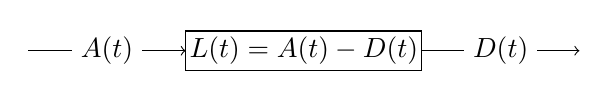
\begin{tikzpicture}[scale=1]
\draw[->] (0,0)--node[midway, fill=white] {$A(t)$}  (2,0); 
\draw (2,-0.25) rectangle node {$L(t)=A(t)-D(t)$} (5,0.25);
\draw[->] (5,0)--node[midway, fill=white] {$D(t)$}  (7,0); 
\end{tikzpicture}
\end{figure}

\noindent What goes in the box (i.e., $A(t)$) and has not yet left
  (i.e., $D(t)$) must be in the box, hence $L(t)=A(t)-D(t)$. 



Let us denote an arrival as an `up-crossing' and a departure as a
`down-crossing'.  Then, clearly $L(t)$ is the number of up-crossings
up to time $t$ minus the number of down-crossings up to time $t$. If
$L(t)$ remains finite, or more generally $L(t)/t \to 0$ as $t\to\infty$, then it
must be that
\begin{equation*}
  \lambda =  \lim_t \frac{A(t)}t  = \lim_t \frac{D(t)+L(t)}t =  \lim_t \frac{D(t)}t + \lim_t \frac{L(t)}t 
  = \delta.  
\end{equation*}
Hence, when $L(t)/t\to0$, the \recall{up crossing rate}
$\lim_t A(t)/t = \lambda$ is equal to the \emph{down-crossing rate}
$\lim_t D(t)/t = \delta$.  We will generalize these notions of up- and
downcrossing in this section to derive the \recall{stationary}---also known as \emph{long-run time average} or \emph{steady-state},
distribution---$p(n)$ that the system contains $n$ jobs. 

\begin{exercise}
  If $L(t)/t \to 0$ as $t\to\infty$, can $\E{L}>0$? 
  \begin{solution}
    \begin{equation*}
      \E{L} = \lim_{t\to\infty} \frac 1 t \int_0^t L(s) \d s \neq \lim_{t\to\infty} \frac{L(t)}t.
    \end{equation*}
If $L(t)=1$ for all $t$, $\E{L} =1 $, but $L(t)/t \to 0$. 
  \end{solution}
\end{exercise}


Let us say that the system is in \emph{state $n$ when it contains $n$
  jobs}, c.f. Figure~\ref{fig:A_n_t}, and the system \emph{crosses}
level $n$ when the state changes from $n$ to $n+1$, either `from
below' when an arrival occurs, or `from above' when a departure
occurs.  The main result we derive in this section is that the rate at
which level $n$ is crossed from below must match the rate at which it is crossed from above, i.e.,
\begin{equation*}
  \lambda(n) p(n) = \mu(n+1) p(n+1),
\end{equation*}
where $\lambda(n)$ is the arrival rate in state $n$, $p(n)$ the
fraction of time the system is in state $n$ and $\mu(n+1)$ the
departure rate from $n+1$. To establish this we need a few definitions
that are quite subtle and might seem a bit abstract, but below we will
provide intuitive interpretations in terms of system KPIs. Once we
have the proper definitions, the above result will follow
straightaway.


Define\footnote{It is common to write
  $f(x+) = \lim_{h\downarrow0} f(x+h)$ for the right limit of a
  function $f$ at $x$ and $f(x-) = \lim_{h\downarrow0} f(x-h)$ for the
  left limit. When $f(x-)=f(x+)$, $f$ is continuous at $x$. Since in
  queueing systems we are concerned with processes with jumps, we need
  to be quite particular about left and right limits at jump epochs.}
\begin{subequations}\label{eq:rates_}
\begin{equation}\label{eq:19} 
  A(n,t) = \sum_{k=1}^\infty \1{A_k \leq t}\1{L(A_k-) = n}
\end{equation}
as the number of arrivals up to time $t$ that saw $n$ customers in the system at their arrival, c.f. Figure~\ref{fig:Y_1_t}.

\begin{exercise}
  Should we  take $L(A_k-)=n$ or $L(A_k)$ in the definition of $A(n,t)$?
  \begin{hint}
Recall that $L(t)$ is \emph{right-continuous}.
  \end{hint}
    \begin{solution}
    $L(t)$ is the number of customers in the system at time $t$. As
    such the function $t\to L(t)$ is \textsl{right-continuous}. The
    definition of $L(A_k-) = \lim_{t\uparrow A_k} L(t)$ is the
    limit from the left.  The customer therefore `sees' $L(A_k-)$ just
    before he arrives. 
\end{solution}  
\end{exercise}

\begin{exercise}
What is the difference between $A(n,t)$ and $A(t)$? 
\begin{solution}
  $A(t)$ counts all customers that arrive up to time $t$, i.e., during
  $[0,t]$. Note that this \textsl{includes} time $t$. $A(n,t)$ counts
  the jobs that see $n$ jobs in the system just before they arrive.
    \end{solution}
\end{exercise}

\begin{exercise}
 Show that $A(n,t) \leq A(t)$. 
\begin{solution}
       Observe that
      $\1{A_k\leq t}\1{L(A_k-) = n} \leq \1{A_k\leq t}$;
      the last inequality follows from the fact that
      $\1{L(A_k-) = n}\leq 1$. Therefore,
    \begin{equation*}
  A(n,t) = \sum_{k=1}^\infty \1{A_k \leq t} \1{L(A_k-) = n} 
\leq \sum_{k=1}^\infty \1{A_k \leq t} = A(t). 
    \end{equation*}
    For any `normal' queueing system, $A(t) > A(t,n)$, because the
    queue length fluctuates.
    \end{solution}
\end{exercise}



\begin{exercise}
  Why is $ \lim_{t\to\infty} \frac{A(n,t)}t = 0$ if
  $\lambda > \delta$, i.e., if the system is not rate-stable?
  \begin{solution}
 If $\lambda > \delta$, then $L(t)\to\infty$. But then there
      must be last time, $s$ say, that $L(s) = n+1$, and $L(t) > n+1$
      for all $t>s$. Hence, after time $s$ no job will see the system
      with $n$ jobs. Thus $A(t,n) = A(s,n)$ for all $t>s$.  This is a
      finite number, while $t\to\infty$, so that $A(n,t)/t \to 0$.
  \end{solution}
 \end{exercise}

Next, let 
\begin{equation} \label{eq:17} 
   Y(n,t) = \int_0^t  \1{L(s) = n} \d s
\end{equation}
be  the total time the system contains n jobs during $[0,t]$, and
\begin{equation} \label{eq:18}
   p(n,t) = \frac 1 t \int_0^t  \1{L(s) = n} \d s = \frac{Y(n,t)}t,
\end{equation}
\end{subequations}
be the fraction of time that $L(s) =n$ in $[0,t]$.
  


\begin{exercise}
  Consider the following (silly) queueing process. At times
  $0, 2,4, \ldots$ customers arrive, each customer requires $1$ unit
  of service, and there is one server. Find an expression for
  $Y(n,t)$.What acronym would describe this queueing situation?
  \begin{hint}
For the acronym, observe that the service times and
    interarrival are \emph{D}eterministic and there is one server. For
    the computation of $Y(n,t)$, make make a plot of $L(s)$ as a
    function of time for $n=1$.
  \end{hint}
    \begin{solution}
      First, it is the $D/D/1$ queue, since there is one server and
      the interarrival times and service times are constant, i.e.,
      \emph{D}eterministic.

      Next, to get $Y(n,t)$, observe that the system never contains
      more than 1 job. Hence, $Y(n,t)=0$ for all $n\geq 2$.  Then,
      make a plot of $L(s)$ for $n=1$ as a function of time.  function
      of time. Then we see that
      $Y(1,t) = \int_0^t \1{L(s) = 1}\d s.$ Now observe that for our
      queueing system $L(s)=1$ for $s\in[0,1)$, $L(s)=0$ for
      $s\in[1,2)$, $L(s)=1$ for $s\in[2,3)$, and so on, Thus, when
      $t<1$, $Y(1,t)=\int_0^t \1{L(s)=1} \d s = \int_0^t 1\d s = t$.
      When $t\in[1,2)$, 
      \begin{equation*}
        L(t)=0 \implies \1{L(t)=0} \implies Y(1,t) \text{ does not change}.
      \end{equation*}
Continuing to $[2,3)$ and so on gives
    \begin{equation*}
      Y(1,t) =
      \begin{cases}
        t &\leq t\in[0,1), \\
        1 &\leq t\in[1,2), \\
        1+(t-2) &\leq t\in[2,3), \\
        2 &\leq t\in[3,4), \\
        2+(t-4) &\leq t\in[4,5), \\
      \end{cases}
    \end{equation*}
    and so on.  Since $Y(n,t)=0$ for all $n\geq 2$, $L(s) = 1$ or
    $L(s)=0$ for all $s$, therefore, 
    \begin{equation*}
      Y(0,t) = t-Y(1,t).
    \end{equation*}
    \end{solution}
\end{exercise}


\begin{figure}[t]
  \centering
\begin{tikzpicture}[scale=1,
  open/.style={shape=circle, fill=white, inner sep=1pt, draw, node contents=},
  closed/.style={shape=circle, fill=black, inner sep=1pt, draw, node contents=},
]

%axis
\draw[->] (0,0) -- coordinate (x axis mid) (8.5,0);
\draw[->] (0,0) -- coordinate (y axis mid) (0,4.5);
%\node[below=0.2cm] at (x axis mid) {$t$};
\node[left=0.3cm, rotate=90] at (y axis mid) {$L(t)$};


\draw 
node (0) at (0,0) [closed] {}
node (c1) at (1,0) [open] {};
\draw[thick] (0)--(c1);
\node[below] at (1,0) {$A_1$};

\draw 
node (c2) at (1,1) [closed] {}
node (c3) at (2.5,1) [open] {};
\draw[thick] (c2)--(c3);
\node[below] at (2.5,0) {$D_1$};

\draw 
node (c2) at (2.5,0) [closed] {}
node (c3) at (3,0) [open] {};
\draw[thick] (c2)--(c3);
\node[below] at (3,0) {$A_2$};

\draw 
node (c2) at (3,1) [closed] {}
node (c3) at (4,1) [open] {};
\draw[thick] (c2)--(c3);

\draw 
node (c2) at (4,2) [closed] {}
node (c3) at (5,2) [open] {};
\draw[thick] (c2)--(c3);
\node[below] at (4,0) {$A_3$};

\draw 
node (c2) at (5,1) [closed] {}
node (c3) at (5.8,1) [open] {};
\draw[thick] (c2)--(c3);
\node[below] at (5.,0) {$D_2$};

\draw 
node (c2) at (5.8,2) [closed] {}
node (c3) at (6.3,2)  {};
\draw[thick] (c2)--(c3);
\node[below] at (5.8,0) {$A_4$};

\draw[dashed] (1,0)--(2.5, 1.5) -- (3, 1.5)--(4,2.5) -- 
(5, 2.5)--(5.8, 3.3)--(6.3, 3.3);
\node[right] at (6.3, 3.3) {$Y(1,t)$};

\draw[dotted] (4,0) -- (4,0.5)--(5.8, 0.5)--(5.8, 1.5)--(6.3, 1.5);
\node[right] at (6.3, 1.5) {$A(1,t)$};

\end{tikzpicture}
  \caption{Plots of $Y(1,t)$ and $A(1,t)$. (For visual clarity, we subtracted $\nicefrac12$ from $A(1,t)$, for otherwise its graph would partly overlap with the graph of $L$.)}
  \label{fig:Y_1_t}
\end{figure}



Define also the limits:
\begin{align*}
  \lambda(n) &= \lim_{t\to\infty} \frac{A(n,t)}{Y(n,t)}, &p(n) &=\lim_{t\to\infty} p(n,t),
\end{align*}
as the \emph{arrival rate in state $n$} and the \emph{long-run fraction of
  time the system spends in state $n$}. To clarify the former
definition, observe that $A(n,t)$ counts the number of arrivals that
see $n$ jobs in the system upon arrival, while $Y(n,t)$ tracks the amount of time
the system contains $n$ jobs. Suppose that at time~$T$ a job arrives that
sees $n$ in the system. Then $A(n,T)=A(n, T-)+1$, and this job finishes
an interval that is tracked by $Y(n,t)$, precisely because this job
sees $n$ in the system just prior to its arrival. Thus, just as
$A(t)/t$ is the total number of arrivals during $[0,t]$ divided by~$t$, $A(n,t)/Y(n,t)$ is the number of arrivals that see $n$ divided by
the time the system contains $n$ jobs.



Similarly, denoting by
\begin{equation*}
    D(n,t) = \sum_{k} \1{D_k \leq t} \1{L(D_k) = n}
  \end{equation*}
  the number of departures up to time $t$ that\emph{ leave $n$
    customers behind}, we define
\begin{equation*}
  \mu(n+1) = \lim_{t\to\infty} \frac{D(n,t)}{Y(n+1,t)},
\end{equation*}
as \emph{ the departure rate from state $n+1$}. (It is easy to get
confused here: to leave $n$ jobs behind, the system must contain $n+1$
jobs just prior to the departure.) Figure~\ref{fig:A_n_t} shows how
$A(n,t)$ and~$\lambda(n)$ relate to $D(n+1,t)$ and $\mu(n)$.

\begin{exercise}
Should  we take $D(n-1,t)$ or  $D(n,t)$ in the definition of $\mu(n)$?
    \begin{solution}
      $D(n-1,t)$ counts the departures that leave $n-1$ behind. Thus,
      just before the customer leaves, the system contains $n$
      customers.
\end{solution}
\end{exercise}


\begin{figure}[th]
  \centering
\begin{tikzpicture}[scale=1,->,>=stealth',shorten >=1pt,auto,node distance=1.8cm,
                    semithick]
  \node[state] (0) {$p(0)$} ;
  \node[state] (1) [right of=0] {$p(1)$};
  \node[state] (2) [right of=1] {$p(2)$};
  \node[state] (3) [right of=2] {$p(3)$};
  \node[state] (4) [right of=3] {$\cdots$};

\path 
 (0) edge [bend left] node {$\lambda(0)$} (1)
 (1) edge [bend left] node {$\mu(1)$} (0)
 (1) edge [bend left] node {$\lambda(1)$} (2)
 (2) edge [bend left] node {$\mu(2)$} (1)
 (2) edge [bend left] node {$\lambda(2)$} (3)
 (3) edge [bend left] node {$\mu(3)$} (2)
 (3) edge [bend left] node {$\lambda(3)$} (4)
 (4) edge [bend left] node {$\mu(4)$} (3);

\draw[-, dotted, gray] (2.7,-2.)--(2.7,2.0) node[above, black] {level $2$};
\draw[->] (2,1.5)  node[left] {$A(1,t)$} -- (3.5,1.5);
\draw[<-] (2,-1.2) node[left] {$D(1,t)$} --(3.5,-1.2) ;

\end{tikzpicture}
\caption{ $A(1,t)$ counts the number of jobs up to time $t$ that saw 1
  job in the system; thus, right after the arrival of such a job the
  system contains 2 jobs. Similarly, $D(1,t)$ counts the number of
  departures that leave 1 job behind.  Each time $A(1,t)$ increases by
  one or $D(1,t)$ decreases by one, level $2$ (the dotted line
  separating states 1 and 2) is crossed.  The number of times this
  level is crossed from below must be the same (plus or minus 1) the
  number of times it is crossed from above. }
\label{fig:A_n_t}
\end{figure}



Observe that customers arrive and depart as single units. Thus, if
$\{T_k\}$ is the ordered set of arrival and departure times of the
customers, then $L(T_k) = L(T_k-) \pm 1$. But then we must also have
that $|A(n,t) - D(n,t)| \leq 1$ (Think about this.). From this
observation it follows immediately that
\begin{equation}\label{eq:15}
  \lim_{t\to\infty} \frac{A(n,t)}t = \lim_{t\to\infty} \frac{D(n,t)}t.
\end{equation}
With this equation we can obtain two nice and fundamental
identities. The first we develop now; the second follows in
Section~\ref{sec:poisson-arrivals-see}.

The rate of jobs that `see the system with $n$ jobs' can be defined as
$A(n,t)/t$. Taking limits we get
\begin{subequations}
\label{eq:21}
\begin{equation}\label{eq:63}
  \frac{A(n,t)}t =   \frac{A(n,t)}{Y(n,t)}\frac{Y(n,t)}t \to \lambda(n) p(n),
\end{equation}
where we use the above definitions for $\lambda(n)$ and $p(n)$.
Similarly, the departure rate of jobs that leave $n$ jobs behind is
\begin{equation}\label{eq:22}
  \frac{D(n,t)}t =   \frac{D(n,t)}{Y(n+1,t)}\frac{Y(n+1,t)}t \to \mu(n+1) p(n+1).
\end{equation}
\end{subequations}
Combining this with~\eqref{eq:15} we arrive at \recall{the
  level-crossing equations}
\begin{equation}\label{eq:12}
  \lambda(n) p(n) = \mu(n+1)p(n+1).
\end{equation}

This result turns out to be exceedingly useful. Once we can specify
$\lambda(n)$ and $\mu(n)$, we can compute the long-run fraction of
time $p(n)$ that the system contains $n$ jobs. To see this, rewrite
the above into
\begin{equation}\label{eq:25}
  p(n+1) = \frac{\lambda(n)}{\mu(n+1)}p(n). 
\end{equation}
Thus, if we have $p(n)$ we can compute $p(n+1)$, and so on. In other
words, if $p(0)$ is known, than $p(1)$ follows, from which $p(2)$
follows, and so on. A straightaway iteration then leads to
\begin{equation}\label{eq:38}
  p(n+1) = \frac{\lambda(n)\lambda(n-1)\cdots \lambda(0)}{\mu(n+1)\mu(n)\cdots \mu(1)}p(0).
\end{equation}
Finally, to determine $p(0)$ we can use the fact that numbers $p(n)$
have to be normalized.  Let the \recall{normalization constant} be given by
\begin{equation}
  \label{eq:20}
G = 1 + \frac{\lambda(0)}{\mu(1)} + \frac{\lambda(0)\lambda(1)}{\mu(1)\mu(2)} + \cdots. 
\end{equation}
Then,  $p(0)=G^{-1}$ and $p(n)$ follows from Eq.~\eqref{eq:38}. 

Let us now express a few important performance measures in terms of
$p(n)$: the average number of items $\E L$ in the system and the
fraction of time $\P{L\leq n}$ the system contains at least $n$ jobs.
As $L(s)$ counts the number of jobs in the system at time $s$ (thus
$L(s)$ is an integer),
\begin{equation*}
  L(s) = \sum_{n=0}^\infty n\, \1{L(s) = n}.
\end{equation*}
With this we can write for the time-average number of jobs in the system
\begin{equation}\label{eq:1}
  \mathscr{L}(t) = \frac 1 t \int_0^t \left(\sum_n n\, \1{L(s) = n}\right) \d s
= \sum_n \frac n t \int_0^t   \1{L(s) = n} \d s,
\end{equation}
where we interchange the integral and the summation\footnote{This is
  allowed as the integrand is non-negative. More generally, the
  interested reader should check Fubini's theorem.}.  It then follows
  from Eq.~(\ref{eq:18}) that
\begin{equation*}
  \mathscr{L}(t) =  \sum_n n\, p(n,t).
\end{equation*}
Finally, assuming that the limit $p(n,t) \to p(n)$ exists as
$t\to\infty$ (and that the summation and limit can be interchanged in
the above), it follows that 
\begin{equation*}
  \mathscr{L}(t) \to  \sum_{n=0}^\infty n p(n) = \E L, \text{ as } t \to \infty.
\end{equation*}
In words, $ \mathscr{L}(t)$ converges to the long-run time average
$\E L$ of the number in the system. In a loose sense we can say that
$\E L$ is the average number in the system as perceived by the
\emph{server}. (Recall that this is not necessarily the same as what
\emph{arriving} jobs `see').  Similarly, the probability that the
system contains at least $n$ jobs is 
\begin{equation*}
  \P{ L \geq n} := \sum_{i=n}^\infty p(i).
\end{equation*}

From the above we conclude that from the probabilities $p(n)$, more
specifically, from a specification of $\lambda(n)$ and $\mu(n)$, we
can compute numerous performance measures. Thus, determining $p(n)$
from Eqs.~\eqref{eq:25} and~\eqref{eq:20} for concrete queueing
examples is the task of the next sections.

Before we embark on this task, we note that the level-crossing cannot
always be used as we do here. The reason is that it is not always
natural, or easy, to decompose the state space into two disjoint
parts. For a more general approach, we focus on a single state and
count how often this state is entered and left,
c.f. Figure~\ref{fig:balance}. Specifically, define
\begin{align*}
  I(n,t) &= A(n-1,t) + D(n,t),
%  O(n,t) &= A(n,t) + D(n-1,t),
\end{align*}
as the number of times the queueing process enters state $n$ either
due to an arrival from state $n-1$ or due to a departure leaving $n$
jobs behind. Similarly,
\begin{align*}
 O(n,t) &= A(n,t) + D(n-1,t),
\end{align*}
counts how often state $n$ is left either by an arrival or a departure
to state $n-1$.

Of course, $|I(n,t)-O(n,t)|\leq 1$. Thus, from the fact that
\begin{equation*}
  \frac{I(n,t)}t = \frac{A(n-1,t)}t + \frac{D(n,t)}t \to \lambda(n-1) p(n-1) + 
\mu(n+1) p(n+1)
\end{equation*}
and 
\begin{equation*}
  \frac{O(n,t)}t = \frac{A(n,t)}t + \frac{D(n-1,t)}t \to \lambda(n) p(n) + 
\mu(n) p(n)
\end{equation*}
we get that
\begin{equation*}
  \lambda(n-1)p(n-1)+\mu(n+1)p(n+1) = (\lambda(n)+\mu(n))p(n).
\end{equation*}
These equations hold for any $n\geq 0$ and are known as the
\recall{balance equations}.  We will use these equations when studying
queueing systems in which level crossing cannot be used, for instance
for queueing networks.

\begin{figure}[t]
  \centering
\begin{tikzpicture}[->,>=stealth',shorten >=1pt,auto,node distance=1.8cm,
                    semithick]
  \node[state] (0) {$p(0)$} ;
  \node[state] (1) [right of=0] {$p(1)$};
  \node[state] (2) [right of=1] {$p(2)$};
  \node[state] (3) [right of=2] {$p(3)$};
  \node[state] (4) [right of=3] {$\cdots$};

\draw[dashed] (2.6,-1.2) rectangle (4.5,1.2);

\path 
 (0) edge [bend left] node {$\lambda(0)$} (1)
 (1) edge [bend left] node {$\mu(1)$} (0)
 (1) edge [bend left] node[fill=white] {$\lambda(1)$} (2)
 (2) edge [bend left] node[fill=white] {$\mu(2)$} (1)
 (2) edge [bend left] node[fill=white] {$\lambda(2)$} (3)
 (3) edge [bend left] node[fill=white] {$\mu(3)$} (2)
 (3) edge [bend left] node[above] {$\lambda(3)$} (4)
 (4) edge [bend left] node[below] {$\mu(4)$} (3);


\end{tikzpicture}
\caption{ For the balance equations we count how often a box around a
  state is crossed from inside and outside. On the long run the
  entering and leaving rates should be equal. For the example here,
  the rate out is $p(2)\lambda(2) + p(2) \mu(2)$ while the rate in is
  $p(1)\lambda(1)+p(3)\mu(3)$.}
\label{fig:balance}
\end{figure}


Again, just by using properties, i.e., counting differences, that hold
along any sensible sample path we obtain very useful statistical and
probabilistic results.


%\nvf{What is valid for ggg1, and what not?, make the assumption explicit for each result.}


\begin{figure}[p]
  \centering

  \begin{tikzpicture}[node distance = 2.5cm]

\tikzset{
    %Define standard arrow tip
    >=stealth',
    %Define style for boxes
    % Define arrow style
    pil/.style={
           ->,
           thick,
           shorten <=2pt,
           shorten >=2pt,}
}
\tikzstyle{block} = [rectangle, draw,text centered, rounded corners, minimum height=3em]

    % nodes
    \node [block, text width=5.5cm, align=center] (level) {LEVEL CROSSING: Counting up- and downcrossings};
\node[block, below=1cm of level] (An) {$|A(n,t)-D(n,t)|\leq 1$}
edge[pil,<-] (level); 

\node[block, left=1.5cm of An] (A) {$|A(t)-D(t)|\leq 1$} 
edge[pil,<-] (level); 

\node[block, right=1.5cm of An] (Anm) {$|A(m,n,t)-D(n,t)|\leq 1$}
edge[pil,<-] (level); 

\node[block, below=1cm of A] (At) {$\frac{A(t)}t \approx \frac{D(t)}t$} 
edge[pil,<-] (A); 

\node[block, below=1.5cm of At] (lambda) {$\lambda=\delta$} 
edge[pil,<-] node[fill=white] {$t\to\infty$} (At); 

\node[block, below=1cm of An] (AnDn) {$\frac{A(n,t)}t\approx\frac{D(n,t)}t$}
edge[pil,<-] (An); 

\node[block, below=1.5cm of AnDn] (AnDn2) {$\frac{A(n,t)}{Y(n,t)}\frac{Y(n,t)}t\approx\frac{D(n,t)}{Y(n+1)}\frac{Y(n+1)}t$}
edge[pil,<-] (AnDn); 

\node[block, below=1.5cm of AnDn2, text width=4cm] (lp) {Recursion: \\
$\lambda(n)p(n) = \mu(n+1)p(n+1)$}
edge[pil,<-] node[fill=white] {$t\to\infty$} (AnDn2); 

\node[block, below=1cm of lp, text width=3cm] (poisson) {Poisson: \\
$\lambda=\lambda(n)$, \\
$\mu=\mu(n)$}
edge[pil,<-] (lp);

\node[block, below=1cm of poisson, text width=4cm] (mm1) {$M/M/1$, $M/M/c$, $M/M/c/k$, \ldots} edge[pil,<-] (poisson);
;

\node[block, right=0.6cm of lp, text width=5cm, align=center] (batch) {Recursion: \\ $\lambda\sum_{m=0}^nG(n-m)p(m) = \mu(n+1)p(n+1)$}
edge[pil,<-] node[fill=white] {$t\to\infty$} (Anm); 

\node[block, right=2.3cm of mm1] (batch2) {$M^X/M/1$}
edge[pil,<-]  (poisson)
edge[pil,<-]  (batch); 


\node[block, below=1cm of mm1, text width=4.5cm] (perf) {Performance
  measures:
$\E L= \sum_{n=0}^\infty n p(n)$, $\P{L\geq m}$, \ldots} 
edge[pil,<-] (mm1)
edge[pil,<-] (batch2);

\node[block, below=1.5cm of lambda] (pasta1) {$\frac{A(t)}t\frac{A(n,t)}{A(t)} = \frac{A(n,t)}{Y(n,t)}\frac{Y(n,t)}t$} 
edge[pil,<-] (AnDn2)
edge[pil,<-,bend left=20] (At.south west)
;

\node[block, below=1.5cm of pasta1] (pasta2) {$\lambda \pi(n) = \lambda(n)p(n)$} 
edge[pil,<-] node[fill=white] {$t\to\infty$} (pasta1);

\node[block, below=1.5cm of pasta2, text width=3cm] (pasta3) {PASTA: $\pi(n) = p(n)$} 
edge[pil,<-] (poisson)
edge[pil,<-] (pasta2)
edge[pil,->] (perf);

\end{tikzpicture}
  \caption{With level-crossing arguments we can derive a number of
    useful relations. This figure presents an overview of these
    relations that we derive in this and the next sections.}
\end{figure}

\paragraph{Interpretation}

The definitions in~(\ref{eq:rates_}) may seem a bit abstract, but they
obtain an immediate interpretation when relating them to
applications. To see this, we discuss two examples.

Consider the sorting process of post parcels at a distribution center
of a post delivery company.  Each day tens of thousands of incoming
parcels have to be sorted to their final destination. In the first
stage of the process, parcels are sorted to a region in the
Netherlands. Incoming parcels are deposited on a conveyor belt. From
the belt they are carried to outlets (chutes), each chute
corresponding to a specific region. Employees take out the parcels
from the chutes and put the parcels in containers.  The arrival rate
of parcels for a certain chute may temporarily exceed the working
capacity of the employees, as such the chute serves as a queue.  When
the chute overflows, parcels are directed to an overflow container and
are sorted the next day. The target of the sorting center is to
deliver at least a certain percentage of the parcels within one
day. Thus, the fraction of parcels rejected at the chute should remain
small.

Suppose a chute can contain at most 20 parcels, say. Then, each parcel
on the belt that `sees' 20 parcels in its chute will be blocked. Let
$L(t)$ be the number of parcels in the chute at time $t$. Then,
$A(20,t)$ as defined in Eq.~(\ref{eq:19}) is number of\emph{ blocked
  parcels} up to time $t$, and $A(20,t)/A(t)$ is the fraction of
rejected parcels. In fact, $A(20,t)$ and $A(t)$ are continuously
tracked by the sorting center and used to adapt employee capacity to
control the fraction of rejected parcels. Thus, in simulations, if one
want to estimate loss fractions, $A(n,t)/A(t)$ is the most natural
concept to consider.

For the second example, suppose there is a cost associated with
keeping jobs in queue. Let $w$ be the cost per job in queue per unit
time so that the cost rate is $n w$ when $n$ jobs are in queue. But
then is $ wnY(n,t)$ the total cost up to time $t$ to have $n$ jobs in
queue, hence the total cost up up to time $t$
  \begin{equation*}
C(t) =     w \sum_{n=0}^\infty n Y(n,t),
  \end{equation*}
and the average cost is
\begin{equation*}
\frac{C(t)}t =    w \sum_{n=0}^\infty n \frac{Y(n,t)}t = w \sum_{n=0}^\infty n p(n,t).
\end{equation*}
All in all, the concepts developed above have natural interpretations
in practical queueing situations; they are useful in theory and in
simulation, as they relate the theoretical concepts to actual measurements.




\begin{exercise}
  Consider a single server that serves one queue and serves only in
  batches of 2 jobs at a time (so never 1 job or more than 2 jobs),
  i.e., the $M/M^2/1/3$ queue.  Single jobs arrive at rate $\lambda$
  and the interarrival times are exponentially distributed. The batch
  service times are also exponentially distributed with mean $1/\mu$.
  At most 3 jobs fit in the system.   Make a graph of the state-space and show, with arrows, the
  transitions that can occur.
  \begin{solution}
\begin{tikzpicture}[scale=1,->,>=stealth',shorten >=1pt,auto,node distance=2.8cm,
                    semithick]
\node[state] (0) {$0$}; 
\node[state] (1) [right of=0] {$1$}; 
\node[state] (2) [right of=1] {$2$}; 
\node[state] (3) [right of=2] {$3$}; 

\path 
(0) edge [bend left] node[above] {$\lambda$} (1)
(1) edge [bend left] node[above] {$\lambda$} (2)
(2) edge [bend left] node[above] {$\lambda$} (3)
(3) edge [bend left] node[below] {$\mu$} (1)
(2) edge [bend left] node[below] {$\mu$} (0);

\draw[-, dotted, gray] (4,-2.)--(4,2.0) node[above, black] {level $1$};

\end{tikzpicture}
  \end{solution}
\end{exercise}

\begin{exercise}
  Use the graph of the previous question and a level-crossing argument
  to express the steady-state probabilities $p(n),n=0,\ldots, 3$ in
  terms of $\lambda$ and $\mu$.
  \begin{hint}
First balance the rates accross the levels. Then solve for $\pi(k)$.
  \end{hint}
  \begin{solution}
With level crossing
  \begin{align*}
    \lambda p(0)  &= \mu p(2) \\
    \lambda p(1)  &= \mu p(2) +\mu p(3), \quad\text{see level 1}\\
    \lambda p(2)  &= \mu p(3)\\
  \end{align*}
  Solving this in terms of $p(0)$ gives $p(2) = \rho p(0)$, $p(3) = \rho p(2) = \rho^2p(0)$, and $p(1) = (\lambda+\mu)/\lambda p(0)$. 
  \end{solution}
\end{exercise}

\Closesolutionfile{hint}
\Closesolutionfile{ans}
\subsection*{Hints}
\input{hint}
\subsection*{Solutions}
\input{ans}
\clearpage

%%% Local Variables:
%%% mode: latex
%%% TeX-master: "book"
%%% End:

 \section
[$M/M/1$ queue]
{$\mathbf{M/M/1}$ queue}
\label{sec:mm1}


\subsection*{Theory and Exercises}

\Opensolutionfile{hint}
\Opensolutionfile{ans}

In the $M/M/1$ queue, one server serves jobs arriving with
exponentially distributed inter-arrival times and each job requires an
exponentially distributed processing time.  With Eq.~(\ref{eq:25}),
i.e., $\lambda(n)p(n)= \mu(n+1)p(n+1)$ we can derive a number of
important results for this queueing process.

Recall from Section~\ref{sec:queu-proc-as} that we can construct the
$M/M/1$ queue as a reflected random walk where the arrivals are
generated by a Poisson process $N_\lambda(t)$ and the departures
(provided the number $L(t)$ in the system is positive) are generated according to the
Poisson process $N_\mu(t)$. Since the rates of these processes do not
depend on the state of the random walk, or the queue for that matter,
$\lambda(n)=\lambda$ for all $n \geq 0$ and $\mu(n)=\mu$ for all $n \geq 1$. Thus, \eqref{eq:25}
reduces to
\begin{equation*}
  p(n+1) = \frac{\lambda(n)}{\mu(n+1)} p(n) = \frac{\lambda}{\mu} p(n) = \rho p(n),
\end{equation*}
where we use the definition of the load $\rho=\lambda/\mu$. Since this
holds for any $n\geq 0$, it follows with recursion that
\begin{equation*}
  p(n+1) = \rho^{n+1} p(0).
\end{equation*}
Then, from the normalization condition
\begin{equation*}
1=  \sum_{n=0}^\infty p(n) = p(0)\sum_{n=0}^\infty \rho^n = \frac{p(0)}{1-\rho},
\end{equation*}
it follows that
\begin{align}\label{eq:23}
p(0) &=1-\rho, &   p(n) &=  (1-\rho)\rho^{n}.
\end{align}

How can we use these equations? First, note that $p(0)$ must be the
fraction of time the server is idle. Hence, the fraction of time the
server is busy, i.e., the utilization, is
\begin{equation*}
  1-p(0) = \rho = \sum_{n=1}^\infty p(n).
\end{equation*}
Here the last equation has the interpretation of the fraction of time
the system contains at least 1 job. 


\begin{exercise}\label{ex:12}
Show that the average number of jobs in an  $M/M/1$ queue is given by
\begin{equation}\label{eq:el}
  \E L = \frac \rho{1-\rho}.
\end{equation}
\begin{hint}
There are various ways to get this result, one is with indicator functions, another with moment generating functions.   
\end{hint}
  \begin{solution}
With indicators, a bit long, but I spell out every step.
\begin{align*}
\E L &= \sum_{n=0}^\infty n p(n) \\
&= \sum_{n=0}^\infty \sum_{i=1}^n \1{i\leq n} p(n)  && n=\sum_{i=1}^n \1{i\leq n}\\
&= \sum_{n=0}^\infty \sum_{i=1}^\infty   \1{i\leq n} p(n)  && i>n\implies \1{i\leq n} = 0\\
&= \sum_{i=1}^\infty \sum_{n=0}^\infty  \1{i\leq n} p(n) &&\text{Fubini} \\
&= \sum_{i=1}^\infty \sum_{n=i}^\infty p(n) && n < i \implies \1{i\leq n}=0 \\
&= \sum_{i=1}^\infty \sum_{n=i}^\infty (1-\rho)\rho^n && p(n) = (1-\rho)\rho^n \\
&= \sum_{i=1}^\infty \sum_{n=0}^\infty (1-\rho)\rho^{n+i} && n\to n+i \\
&= \sum_{i=1}^\infty (1-\rho)\rho^i \sum_{n=0}^\infty \rho^n && \rho^{n+i}=\rho^i \rho^n\\
&= \sum_{i=1}^\infty (1-\rho)\rho^i \frac1{1-\rho}   \\
&= \sum_{i=1}^\infty \rho^i \\
&= \sum_{i=0}^\infty \rho^{i+1} && i\to i+1\\
&= \rho \sum_{i=0}^\infty \rho^i \\
&= \frac{\rho}{1-\rho}.
\end{align*}
Note that, since the summands are positive, we can use Fubini's theorem
to justify the interchange of the summations.

With moment generating functions it is a bit shorter. 
\begin{equation*}
  \begin{split}
  M_L(s) 
&= \E{e^{s L}} = \sum_{n=0}^\infty e^{s n}p(n) = (1-\rho) \sum_n e^{s n} \rho^n \\
&=\frac{1-\rho}{1-e^{s}\rho},
  \end{split}
\end{equation*}
where we assume that $s$ is such that $e^s \rho < 1$. Then, 
\begin{equation*}
  M_L'(s) = (1-\rho) \frac{1}{(1-e^s\rho)^2} e^s \rho.
\end{equation*}
Hence, $\E L = M_L'(0) = \rho/(1-\rho)$.
  \end{solution}
\end{exercise}

From the previous exercise, it follows that
\begin{equation*}
 \E L \sim \frac 1{1-\rho}, \quad \text{ as }\rho\to 1..
\end{equation*}
Let us interpret this expression. The fact
that $\E L \sim (1-\rho)^{-1}$ for $\rho\to 1$ implies that the
average waiting time increases very fast when $\rho\to1$.  If we want to avoid  long waiting times, this formula tells us that  situations with
$\rho\approx 1$ should be avoided. As a practical guideline, it is typically best to  keep $\rho$ quite a bit below 1, and accept that servers are not fully  utilized. 


\begin{exercise}
  Show that the excess probability, i.e., the probability that a long queue occurs, is 
$\P{L\geq n} = \rho^n$.
  \begin{hint}
$\P{L\geq n} = \sum_{k\geq n} p(k)$.
  \end{hint}
  \begin{solution}
    \begin{equation*}
      \begin{split}
 \P{L\geq n} 
 &= \sum_{k=n}^\infty p(k) = \sum_{k=n}^\infty p(0)\rho^k = (1-\rho)\sum_{k=n}^\infty \rho^k \\
 &= (1-\rho)\rho^n \sum_{k=0}^\infty\rho^k = (1-\rho) \rho^n \frac1{1-\rho}.
\end{split}
\end{equation*}
\end{solution}
\end{exercise}

Clearly,  the probability that the queue length exceeds some threshold decreases geometrically fast (for  $\rho<1$). If we make the simple assumption
that customers decide to leave (or rather, not join) the system when
the queue is longer than $9$ say, then $\P{L\geq 10} = \rho^{10}$ is
an estimator of the fraction of customers lost. 

% In the context of inventory theory these equations are particularly
% useful, see one of the questions below.


\paragraph{Relation between Inventory and Queueing Systems}

There exists an interesting relation between inventory and queueing systems, c.f. Figure~\ref{fig:inv_queue}.  When a job arrives in the queueing system, the virtual workload~$V(t)$ increases by the service time of the job. In the inventory system, the inventory $I(t)$ decreases by the  demand size of the customer. Like this, the demand size of a customer at the inventory system converts into a production time (i.e., a service time) of a job at a queueing  system. In the figure, the demand size $D_1$  of the first customer corresponds to a production time of duration  $S_1=D_1$, and so on. Thus, even though in the inventory system, customers do not have to wait, their demands spawn production times at a server who has to replenish the consumed items. 

Assume now that  the inventory process is controlled by an order-up-to policy: produce (refill the inventory) as long as the inventory level is below $S$ and stop otherwise.  Then the figure shows that the inventory level $I(t)$ is equal to $S-V(t)$.   

In more general terms, in a queueing system or an inventory system, there is always `something' or `somebody'  waiting. Items in a supermarket are produced ahead of the moment they are `consumed', hence they `wait' for customers. In a queueing system, customers are waiting  while their product is `produced' by the server. When there are no customers in a queueing system, the server waits until a new customers comes along. Thus, queueing and inventory theory are both focused on the distribution of waiting times, either by customers, servers, or items, hence  both are related branches of (applied) probability theory.


\begin{figure}[th]
\begin{center}
\begin{tikzpicture}[yscale=0.5]
\draw[->] (0,0) -- coordinate (x axis mid) (8.5,0);
\draw[->] (0,0) -- coordinate (y axis mid) (0,10.5);
\node[below=0.2cm] at (x axis mid) {$t$};

\draw plot coordinates {(1,0) (1,2) (2,1) (2,4) (4,2) (4,4.2) (7.5,0)};
\node[left]  at (7,2.5) {$V(t)$};
\node[fill=white, rotate=90]  at (1,1) {$S_1$};
\node[fill=white, rotate=90]  at (2,2.5) {$S_2$};
\node[fill=white, rotate=90]  at (4,3.) {$S_3$};

\node  at (7,5) {$V(t)=S-I(t)$};

\draw[dotted] (0,10)--(8.5,10);
\node[left]  at (0,10) {$S$};
\node[left]  at (7,7.5) {$I(t)$};
\draw plot coordinates {(1,10) (1,8) (2,9) (2,6) (4,8) (4,6.0) (7.5,10)};
\node[fill=white, rotate=90]  at (1,9) {$D_1$};
\node[fill=white, rotate=90]  at (2,7.5) {$D_2$};
\node[fill=white, rotate=90]  at (4,7) {$D_3$};
\end{tikzpicture}
\end{center}
\caption{The relation between inventory and queueing systems. Here $I(t)$ models the evolution of the inventory level in an  inventory system, while $V(t)$ shows the virtual workload, and $S$ is the order up to level. When a customer requires $D_1$ items, say, it takes a server of a time $S_1=D_1$ to produce these items. Thus, demands at the inventory system convert into production times in a queueing system.  When the inventory is always replenished to level $S$, then the shortage of the inventory level relative to $S$, i.e., $S-I(t)$, becomes the workload $V(t)$ for the server in terms of amount of items or production time.} \label{fig:inv_queue}
\end{figure}


\begin{exercise}\label{ex:7}
Customers of fast-food restaurants prefer to be served from stock. For this reason such
restaurants often use a `produce-up-to' policy: When the on-hand inventory $I$ is equal or lower than some threshold $S-1$, the company produces items until the inventory level equals $S$ again. The level $S$ is known as the order-up-to level, and $S-1$ as the reorder level.

Suppose that customers arrive as a Poisson process with rate $\lambda$
and the production times of single items are i.i.d. and exponentially
distributed with parameter $\mu$. Assume also that customers who
cannot be served from on-hand stock are backlogged, that is, they wait
until their item has been produced. What are the average on-hand
inventory level and the average number of customer in backlog?
\begin{hint}
Use Figure~\ref{fig:inv_queue} to realize that the inventory level $I(t)$ (here measured in the number of items on stock) at time $t$ can be
  modeled as $I(t) = S+1-L(t)$, where $L$ is the number of jobs in an
  $M/M/1$ queue. Note that the number of jobs in queue corresponds to the number of items to be produced. A customer of an item, i.e., a demand of the inventory system, turns into  job at the queueing system, i.e., the demand becomes a job for the cook to replenish the item.
\end{hint}
  \begin{solution}
In the $M/M/1$ queue, $p(n)$ corresponds to the fraction of time there are $n$ jobs in the system. In the inventory system, it means that the cook has $n$ jobs to satisfy, hence the inventory is $n$ jobs short relative to the order up to level $S$.  Hence, the average on-hand inventory is $S$ minus the average number of jobs at the cook. i.e., $\E{I} = \sum_{i=0}^{S} (S-i) p(i)$. The average number of customers in backlog is the fraction of time there are more than $S$ replenishment jobs at the cook, i.e., $\E B = \sum_{i=S+1}^\infty (i-S) p(i)$. 
  \end{solution}
\end{exercise}


\paragraph{Supermarket Planning}

Let us consider the example of cashier planning of a supermarket to
demonstrate how to use the tools we developed up to now. Out of
necessity, our approach is a bit heavy-handed---Turning the example
into a practically useful scheme requires more sophisticated queueing
models and data assembly---but the present example contains the
essential analytic steps to solve the planning problem.

The \emph{service objective} is to determine the minimal service
capacity $c$ (i.e. the number of cashiers) such that the fraction of the time more than 
10 people in queue is less than 1\%. (If the supermarket has 3 cashiers open, 10 people in queue  means about 3 people per queue.)

The next step is to find the \emph{relevant data}: the arrival process and the service time distribution. For the arrival process it is reasonable to model it as a Poisson process. There are many potential customers, each choosing with small probability to go the supermarket on a certain moment in time. Thus, we only have to  characterize the arrival rate. Estimating this for a supermarket  is relatively easy: the cash registers track all customers
payments. Thus, we know the number of customers that left the shop,
hence entered the shop. (We neglect the time customers spend in the
shop.) Based on these data we make a \emph{demand profile}: the
average number of customers arriving per hour, c.f. Figure~\ref{fig:loadprofile}. Then we model the arrival process as Poisson with an arrival rate that is constant during a certain hour and is specified by the demand profile, 

\begin{figure}[t]
  \centering
\begin{tikzpicture}[scale=.7]
 	%axis
	\draw[->] (0,0) -- coordinate (x axis mid) (13.5,0);
    	\draw[->] (0,0) -- coordinate (y axis mid) (0,5.5);
    	%ticks
    	\foreach \x in {0,...,13}
        \pgfmathsetmacro{\my}{int(\x+8)}
     		\draw (\x,1pt) -- (\x,-3pt)
			node[anchor=north] {$\my$};
    	\foreach \y in {0,...,5}
        \pgfmathsetmacro{\my}{int(\y*40)}
     		\draw (1pt,\y) -- (-3pt,\y) 
     			node[anchor=east] {\my}; 
%labels      
\node[below=0.6cm] at (x axis mid) {hour};
\node[rotate=90, left=1.2cm] at (y axis mid) {$\lambda$};

\draw (0,1)--(1,1);
\draw (1,2)--(2,2);
\draw (2,2.6)--(3,2.6);
\draw (3,2.8)--(4,2.8);
\draw (4,3.)--(5,3.);
\draw (5,3.1)--(6,3.1);
\draw (6,2.7)--(7,2.7);
\draw (7,1.9)--(8,1.9);
\draw (8,2.5)--(9,2.5);
\draw (9,3.3)--(10,3.3);
\draw (10,3.5)--(11,3.5);
\draw (11,2.3)--(12,2.3);
\draw (12,1.2)--(13,1.2);
\end{tikzpicture}
  \caption{A  demand profile of the arrival rate $\lambda$ modeled as constant over each hour.}
  \label{fig:loadprofile}
\end{figure}


It is also easy to find the service distribution from the cash
registers. The first item scanned after a payment determines the start
of a new service, and the payment closes the service. (As there is
always a bit of time between the payment and the start of a new
service we might add 15 seconds, say, to any service.)
To keep things simple here, we just model the service time distribution as
exponential with a mean of $1.5$ minutes. 

We also \emph{model} the behavior of all the cashiers together (a multi-server queue) as a single fast server. Thus, we neglect any differences between a station with, for instance, 3 cashiers and a
single server that works 3 times as fast as a normal cashier.  As yet
another simplification, we change the objective somewhat such that the
number of jobs in the system, rather than the number in queue, should not exceed 10. 

We now find a formula to convert the demand profile into the \emph{load profile}, which is the minimal number of servers per hour needed to meet the service objective. We already know for the $M/M/1$ that $\P{L>10}=\rho^{11}$.  Combining this with the objective $\P{L>10}\leq 1\%$, we get that $\rho^{11}\leq 0.01$, which  translates into $\rho \leq 0.67$. Using that $\rho = \lambda \E S/c$ and our estimate $\E{S}=1.5$ minutes,  we get  the following rough bound on $c$:
\begin{equation*}
c \geq \frac{\lambda \E S}{0.67} \approx \frac{3}2 \cdot \lambda \cdot 1.5  \approx 2.5 \lambda,
\end{equation*}
where $\lambda$ is the arrival rate (per minute, \emph{not} per hour).
For instance, for the hour from 12 to 13, we read in  the demand profile that $\lambda= 120$ customers per hour, hence $c=2.5 \cdot 120/60 = 5$. With this formula, the conversion of the demand profile to the load profile becomes trivial: divide the hourly arrival rate by $60$ and multiply by
$2.5$.

The last step is to \emph{cover the load profile with service shifts}. This
is typically not easy since shifts have to satisfy all kinds of rules,
such as: after 2 hours of work a cashier should take a break of at least
10 minutes; a shift length must be at least four hours, and not longer
than 9 hours including breaks; when the shift is longer than 4 hours
it needs to contain at least one break of 30 minutes; and so on. These
shifts also have different costs: shifts with hours after 18h
are more expensive per hour; when the supermarket covers traveling
costs, short shifts have higher marginal traveling costs; and so on.

The usual way to solve such  covering problems is by means of an integer
problem. First generate all (or a subset of the) allowed shift types
with associated starting times. For instance, suppose only 4 shift
plans are available
\begin{enumerate}
\item $++-++$
\item $+++-+$
\item $++-+++$
\item $+++-++$,
\end{enumerate}
where a $+$ indicate a working hour and $-$ a break of an hour. Then
generate shift types for each of these plans with starting times
$8$am, $9$am, and so on, until the end of the day. Thus, a shift type
is a shift plan that starts at a certain hour. Let $x_i$ be the number
of shifts of type $i$ and $c_i$ the cost of this type. Write $t\in s_i$ if
hour $t$ is covered by shift type $i$.  Then the problem is to solve
\begin{equation*}
  \min \sum_i c_i x_i.
\end{equation*}
such that 
\begin{equation*}
  \sum_i x_i \1{t \in s_i} \geq 2.5 \frac{\lambda_t}{60}
\end{equation*}
for all hours $t$ the shop is open and $\lambda_t$ is the demand for
hour $t$.




\Closesolutionfile{hint}
\Closesolutionfile{ans}

\opt{solutionfiles}{
\subsection*{Hints}
\input{hint}
\subsection*{Solutions}
\input{ans}
}



%%% Local Variables:
%%% mode: latex
%%% TeX-master: "../queueing_book"
%%% End:

%  \section
[$M(n)/M(n)/1$ Queue]
{$\mathbf{M(n)/M(n)/1}$ Queue}
\label{sec:mnmn1}

As it turns out, many more single-server queueing situations can be
modeled and analyzed by making a judicious choice of $\lambda(n)$ and
$\mu(n)$ in~\eqref{eq:25}, to wit,
$ \lambda(n) p(n) = \mu(n+1)p(n+1)$. For these queueing systems we
just present the results. In the exercises we ask you to derive the
formulas.

For the $M/M/1/K$, i.e., a system that cannot contain more than $K$ jobs, take
  \begin{align*}
    \lambda(n) &= 
  \begin{cases}
    \lambda, &\text{ if } n < K, \\
    0, &\text{ if } n \geq K, \\
  \end{cases} \\
\mu(n) &= \mu.
  \end{align*}
  Then,
\begin{subequations}\label{eq:8}
 \begin{align}
p(n) &=  \frac{\rho^n}G, \quad 0\leq n \leq K,\\
G &= \frac{1-\rho^{K+1}}{1-\rho}, \\
P_{\text{loss}} &= \P{L=K} = \frac{\rho^K}G = \frac{1-\rho}{1-\rho^{K+1}} \rho^K.
\end{align}
\end{subequations}


For the $M/M/c$ queue we can take
  \begin{align*}
\lambda(n) &= \lambda, \\
    \mu(n) &= 
  \begin{cases}
    n\mu, &\text{ if } n < c, \\
    c\mu, &\text{ if } n \geq c.
  \end{cases}
  \end{align*}
This model is also known as the \recall{Erlang $C$}-formula. 
Define the load as 
\begin{subequations}\label{eq:9}
\begin{equation*}
  \rho = \frac{\lambda}{c\mu}.
\end{equation*}
  Then,
 \begin{align}
p(n) &= \frac{1}G \frac{(c\rho)^n}{n!}, \quad n=0,\ldots, c-1 \\
p(n) &= \frac{1}G \frac{c^c\rho^n}{c!}, \quad n=c,c+1, \ldots \\
G &=\sum_{n=0}^{c-1} \frac{(c\rho)^n}{n!} + \frac{(c\rho)^c}{(1-\rho)c!}, \label{eq:501}\\
\E{L_Q} &= \sum_{n=c}^\infty (n-c) p(n) = \frac{(c\rho)^c}{c! G}\frac{\rho}{(1-\rho)^2}, \\ 
\E{L_S} &= \sum_{n=0}^{c-1}n p(n) = \frac{\lambda}\mu.
\end{align}
\end{subequations}
By taking the limit $c\to\infty$ we obtain the $M/M/\infty$ queue, in which case
\begin{subequations}
 \begin{align} 
\rho &= \frac{\lambda}\mu\\
p(n) &=  \frac 1 G\frac{\rho^n}{n!}\\
G &= e^{\rho} \\
\E{L} &= \E{L_S} = \rho.
\end{align}
\end{subequations}

A model, often used to determine the number of beds at hospitals, is
the $M/M/c/c$ model, also known as the Erlang $B$-formula; here jobs cannot be in queue, only in service, and the system has $c$ servers.


Finally, we consider queues with \recall{balking}, that is, queues in
which customers leave when they find the queue too long at the moment
they arrive. A simple example model with  customer balking is given by x
  \begin{equation*}
    \lambda(n) = 
  \begin{cases}
    \lambda, &\text{ if } n=0, \\
    \lambda/2, &\text{ if } n=1, \\
    \lambda/4, &\text{ if } n=2, \\
    0, &\text{ if } n > 2, \\
  \end{cases}
  \end{equation*}
and $\mu(n)=\mu$.   

Observe that in the example with balking we made a subtle implicit
assumption; in Section~\ref{sec:poisson-arrivals-see} we elaborate on
this assumption. To make the problem clear, note that balking
customers \emph{decide at the moment they arrive} to either join or
leave; in other words, they decide based on what they `see upon
arrival'. In yet other words, they make decisions based on the state
of the system at arrival moments, not on time-averages. However, the
notion of $p(n)$ is a long-run \emph{time-average}, and is typically
not the same as what customers `see upon arrival'. As a consequence,
the performance measure $\P{L\leq n}$ is not necessarily in accordance
with the perception of customers. To relate these two `views', i.e.,
time-average versus observer-average, we need a new concept,
\emph{PASTA}, to be developed in in Section~\ref{sec:poisson-arrivals-see}.

\begin{question}
Consider the $M/M/2/2+1$ queue with arrival rate $\lambda$ and
service rate $\mu$. 
\begin{enumerate}
\item Derive the level-crossing equations for this queueing system. 
\item Derive a simple and closed form expressions for the state 
   probabilities in steady state. 
 \end{enumerate}
 
 \hint{Think about what would be the appropriate model choices for
   $\lambda(n)$ and $\mu(n)$ and use the level-crossing equations
   $\lambda(n) p(n) = \mu(n+1)p(n+1)$.  For instance, realize that
   $\lambda(3)=0$: the system cannot contain more than 3 jobs, hence a
   state with $4$ jobs must be impossible. We can achieve that by
   setting $\lambda(3)=0$. For the service rate, how many servers are
   busy when the system contains 2 or more jobs?  What does this say
   about $\mu(k)$ for $k=2$ or $k=3$.}

  \begin{solution}

    \begin{enumerate}
    \item Use this figure. Make sure you understand why $\mu(2)=2\mu$ and so on. 


    \begin{center}

\begin{tikzpicture}[->,>=stealth',shorten >=1pt,auto,node distance=1.8cm,
                    semithick]
  \node[state] (0) {$p(0)$} ;
  \node[state] (1) [right of=0] {$p(1)$};
  \node[state] (2) [right of=1] {$p(2)$};
  \node[state] (3) [right of=2] {$p(3)$};

\path 
 (0) edge [bend left] node {$\lambda$} (1)
 (1) edge [bend left] node {$\mu$} (0)
 (1) edge [bend left] node {$\lambda$} (2)
 (2) edge [bend left] node {$2\mu$} (1)
 (2) edge [bend left] node {$\lambda$} (3)
 (3) edge [bend left] node {$2\mu$} (2);
\end{tikzpicture}
      
    \end{center}

From this figure it follows right away that:
    \begin{align*}
   \lambda p(0) &= \mu p(1) \\
   \lambda p(1)  &= 2\mu p(2) \\
   \lambda p(2)  &= 2\mu p(3)\\
    \end{align*}

  \item From the above, with $\rho=\lambda/\mu$: 
    \begin{align*}
      p(1) &= \rho p(0), \\
      p(2) &= (\rho/2) p(1) = (\rho^2/2) p(0), \\
      p(3) &= (\rho/2) p(2) = (\rho^3/4) p(0).
    \end{align*}
Now we normalize to find $p(0)$. Thus, we want that:
\begin{equation*}
  1 = p(0)+p(1)+p(2)+p(3) = p(0)\left(1 + \rho + \frac{\rho^2}2 + \frac{\rho^3}4\right),
\end{equation*}
hence,
\begin{equation*}
p(0) = (1+\rho + \rho^2/2 + \rho^3/4)^{-1}.
\end{equation*}
\end{enumerate}
   \end{solution}
\end{question}


\begin{question}
  \begin{enumerate}
  \item Derive Eq.~\eqref{eq:8}
  \item   Show that as $K\to\infty$, the performance measures of the $M/M/1/K$ converge to those of the $M/M/1$ queue. 
  \end{enumerate}
  \hint{Use that $\sum_{i=0}^n x^i = (1-x^{n+1})/(1-x)$. BTW, is it
    necessary for this expression to be true that $|x|<1$? What should
    you require for $|x|$ when you want to take the limit
    $n\to\infty$?}
  \begin{solution}
Note that 
\begin{equation*}
1 = \sum_{i=0}^K p(i) = p(0)\sum_{i=0}^K \rho^i  = p(0) \frac{1-\rho^{K+1}}{1-\rho}. 
\end{equation*}
Thus, for the normalization constant $G$ we take 
\begin{equation*}
G=\frac 1{p(0)} = \frac{1-\rho^{K+1}}{1-\rho},
\end{equation*}
and the result follows. 

To take the limit $K\to\infty$---mind, not the limit $n\to\infty$---, write
\begin{equation*}
G= \frac{1-\rho^{K+1}}{1-\rho} = \frac{1}{1-\rho} -\frac{\rho^{K+1}}{1-\rho}.
\end{equation*}
Since $\rho^{K+1}\to 0$ as $K\to \infty$ (recall, $\rho<1$),  we get
\begin{equation*}
G \to \frac{1}{1-\rho}, 
\end{equation*}
as $K\to\infty$.  Therefore $p(n)=\rho^n/G \to \rho^n(1-\rho)$, and
the latter are the steady-state probabilities of the $M/M/1$
queue. Finally, if the steady state probabilities are the same, the
performance measures (which are derived from $p(n)$) must be the same.
  \end{solution}
\end{question}

\begin{question}(Multi-server queue with blocking) Consider the
  $M/M/c/c+K$ queue, try to derive the steady state probabilities
  $p(0)$, $p(1), \ldots$. You do not have to compute the normalization
  constant $G$.

\hint{ Use $\lambda(n) p(n) = \mu(n+1)p(n+1)$ and
    find suitable expressions for $\lambda(n)$ and $\mu(n+1)$. }

  \begin{solution}
    $\lambda(n) \equiv \lambda$ for all $n<c+K$. When $n=c+K$,
    $\lambda(n)=0$, since then the system is full, and all arriving
    jobs will be dropped; in other words, there will still be jobs
    arriving to the system when $L=c+K$, but these jobs will be
    rejected, hence cannot generate a transition from state $c+K$ to
    $c+K+1$.  When $n<c$, $\mu(n)=n \mu$ since only $n$ servers
    are active/occupied when the system contains $n$ jobs. When
    $n\geq c$, $\mu(n) = c \mu$. Thus, using $\rho=\lambda/(c\mu)$, for $n<c$,
     \begin{equation*}
      p(n) = \frac{\lambda}{n\mu} p(n-1) = \frac{(\lambda/\mu)^n}{n!} p(0)=\frac{(c\rho)^n}{n!}p(0).
     \end{equation*}
For $c\leq n\leq c+K$ and using the above to get $p(c-1)$:
 \begin{equation*}
   \begin{split}
 p(n) &= \frac{\lambda}{c\mu} p(n-1) 
= \rho p(n-1) = \rho^2 p(n-2) = \ldots\\
&=\rho^{n-c+1} p(c-1) 
=\rho^{n-c+1} \frac{(c\rho)^{c-1}}{(c-1)!}p(0)\\
&=\rho^{n} \frac{(c)^{c-1}}{(c-1)!}p(0) 
=\rho^{n} \frac{(c)^{c-1}c}{(c-1)!c}p(0) =\frac{c^c \rho^n}{c!} p(0).
   \end{split}
 \end{equation*}
The normalization is trivial, numerically at least.
  \end{solution}
\end{question}

\begin{question}
  Check that  Eq.\eqref{eq:9} for the $M/M/c$ queue reduces to the $M/M/1$ queue if you take $c=1$.
\hint{Fill in $c=1$. Realize that this is a check on the formulas.}
  \begin{solution}
Take $c=1$
 \begin{align}
p(0) &= \frac{1}G \frac{(c\rho)^0}{0!}=\frac1 G, \quad n=0,\ldots, 1-1 \\
p(n) &= \frac{1}G \frac{c^c\rho^n}{c!} = \frac{1}G \frac{1^1\rho^n}{1!} =\frac{\rho^n}G , \quad n=1,1+1, \ldots \\
G &=\sum_{n=0}^{c-1} \frac{(c\rho)^n}{n!} + \frac{(c\rho)^c}{(1-\rho)c!}
=\sum_{n=0}^{0} \frac{\rho^0}{0!} + \frac{\rho}{(1-\rho)} = 1 + \frac{\rho}{1-\rho} = \frac1{1-\rho}
\\
\E{L_Q} &= \frac{(c\rho)^c}{c! G}\frac{\rho}{(1-\rho)^2} = 
= \frac{\rho}{1/(1-\rho)}\frac{\rho}{(1-\rho)^2} = \frac{\rho^2}{1-\rho} \\
\E{L_S} &= \sum_{n=0}^{c-1}n p(n) = \frac{\lambda}\mu = \rho.
\end{align}
Everything is in accordance to the formulas we derived earlier for the $M/M/1$ queue.    
  \end{solution}
\end{question}

\begin{question}
  Derive Eq.\eqref{eq:9} for the $M/M/c$ queue.

  \hint{ Use $\lambda(n)p(n) = \mu(n+1)p(n+1)=\min\{c, n+1\}\mu p(n+1)$.}

  \begin{solution}
First we use the hint to  establish a generic relation for $p(n+1)$:
    \begin{equation*}
      \begin{split}
       p(n+1) 
&= \frac{\lambda}{\mu(n+1)}p(n) 
= \frac{\lambda}{\min\{c, n+1\} \mu }p(n) \\
&= \frac{1}{\min\{c, n+1\}}\frac\lambda\mu p(n) 
= \frac{1}{\min\{c, n+1\}}(c\rho) p(n) \\
&= \frac{1}{\min\{c, n+1\}\min\{c, n\}}(c\rho)^2 p(n-1) 
= \frac{1}{\Pi_{k=1}^{n+1}\min\{c, k\}}(c\rho)^{n+1} p(0).
      \end{split}
    \end{equation*}
Thus, if $n<c$:
\begin{equation*}
  p(n) = \frac{1}{\Pi_{k=1}^{n}\min\{c, k\}}(c\rho)^{n} p(0) = \frac{(c\rho)^n}{n!} p(0),
\end{equation*}
since $\min\{c,k\}=k$ when $k<c$. If $n\geq c$:
\begin{equation*}
  \begin{split}
  p(n) 
&= \frac{1}{\Pi_{k=1}^{n}\min\{c, k\}}(c\rho)^{n} p(0) \\
&= \frac{1}{\Pi_{k=1}^{c-1} k \cdot \Pi_{k=c}^{n} c}(c\rho)^{n} p(0) \\
&= \frac{1}{(c-1)! c^{n-c+1}}c^n\rho^{n} p(0) \\
&= \frac{1}{c! c^{n-c}}c^n\rho^{n} p(0) = \\
&= \frac{c^c}{c!}\rho^{n} p(0).
  \end{split}
\end{equation*}


For the normalization constant $G$ set $p(0)=1$ for the time being. 
\begin{equation*}
  \begin{split}
G &= \sum_{n=0}^\infty p(n) 
= \sum_{n=0}^{c-1} p(n) + \sum_{n=c}^\infty p(n) \\
&=\sum_{n=0}^{c-1}\frac{(c\rho)^n}{n!} + 
 \sum_{n=c}^{\infty} \frac{c^c}{c!} \rho^{n}  \\
&=\sum_{n=0}^{c-1}\frac{(c\rho)^n}{n!} + 
 \sum_{n=c}^{\infty} \frac{(c\rho)^c}{c!} \rho^{n-c}  \\
&= 
\sum_{n=0}^{c-1}\frac{(c\rho)^n}{n!} + 
\frac{(c\rho)^c}{c!} \sum_{n=0}^{\infty} \rho^n \\
&= 
\sum_{n=0}^{c-1}\frac{(c\rho)^n}{n!} + 
\frac{(c\rho)^c}{c!(1-\rho)}.
  \end{split}
\end{equation*}


Next, 
\begin{equation*}
  \begin{split}
  \E{L_Q} 
&=\sum_{n=c}^\infty (n-c) p(n) \\
&=\sum_{n=c}^\infty (n-c) \frac{c^c}{c!}\rho^{n} p(0) \\
&=\frac{c^c\rho^c}{Gc!} \sum_{n=c}^\infty (n-c) \rho^{n-c} \\
&=\frac{c^c\rho^c}{Gc!} \sum_{n=0}^\infty n \rho^n 
=\frac{c^c\rho^c}{Gc!} \frac{\rho}{(1-\rho)^2},
  \end{split}
\end{equation*}
where, with our common trick (if we don't want to use generating functions),
\begin{equation*}
  \begin{split}
  \sum_{n=0}^\infty n \rho^n 
&= \sum_{n=0}^\infty \sum_{i=1}^\infty \1{i\leq n} \rho^n
= \sum_{i=1}^\infty   \sum_{n=0}^\infty \1{i\leq n} \rho^n\\
&= \sum_{i=1}^\infty   \sum_{n=i}^\infty \rho^n
= \sum_{i=1}^\infty   \rho^i \sum_{n=0}^\infty \rho^n\\
&= \frac1{1-\rho} \sum_{i=1}^\infty   \rho^i 
= \frac\rho{1-\rho} \sum_{i=0}^\infty   \rho^i 
= \frac\rho{(1-\rho)^2}.
  \end{split}
\end{equation*}
Observe again that using indicators and Fubini's theorem
(interchanging summations/integrals) makes the above computation
painless. Realize, by the way, that
\begin{equation*}
  \sum_{n=0}^\infty n p(n) = \sum_{n=1}^\infty n p(n).
\end{equation*}

We next show that the expected number of jobs in service is given
by
    \begin{equation*}
      \E{L_S} = \sum_{n=0}^{c-1} n p(n) + \sum_{n=c}^{\infty} c p(n).
    \end{equation*}
    This expression is not the easiest to start with. With a slight
    modification the entire derivation becomes easier. I also premultiply by the normalization constant $G$ to get rid of it on the right hand side. 
    \begin{equation*}
      \begin{split}
      G \E{L_S}
&= G \sum_{n=0}^{c} n p(n) + \sum_{n=c+1}^{\infty} c p(n) \\
&= \sum_{n=1}^{c} n \frac{(c\rho)^n}{n!}  + \sum_{n=c+1}^{\infty} c \frac{c^c\rho^n}{c!} 
= \sum_{n=1}^{c} \frac{(c\rho)^n}{(n-1)!}  + \frac{c^{c+1}}{c!}\sum_{n=c+1}^{\infty} \rho^n\\
&= \sum_{n=0}^{c-1} \frac{(c\rho)^{n+1}}{n!}  + \frac{(c\rho)^{c+1}}{c!}\sum_{n=0}^{\infty} \rho^n
= c\rho \left(\sum_{n=0}^{c-1} \frac{(c\rho)^n}{n!}  + \frac{(c\rho)^{c}}{c!(1-\rho)}\right).
      \end{split}
    \end{equation*}
Observe that the right hand side is precisely equal to $\rho c G$, and hence,
\begin{equation*}
  \E{L_S} = c\rho = \frac\lambda\mu.
\end{equation*}
\end{solution}
\end{question}



\begin{question}[use=false]
  \TBD.  Explain the difference between level crossing and balance
  equations, and the pros and cons of each.
\end{question}

\begin{question}[use=false]
  The ANWB offers roadside assistance to motorists that got stranded
  somewhere along the highway. Suppose that the average repair time
  (including travel time) is 1.5 hour. The ANWB strives to keep the
  average time between receiving a phone call and the actual
  appearance of a mechanic below one hour. Assuming that the average
  travel time to a customer is half an hour, the average waiting time
  must be kept below half an hour. How many mechanics should be
  available if the `arrival rate' of broken cars is $\lambda = 1$ per
  hour? Make a plot of the number of mechanics required as a function
  of $\lambda$ for $\lambda \in [1, 12]$ per hour. 

  Make the assumption that the arrival process of breakdowns is
  Poisson distributed and the repair times are exponentially distributed..
  \begin{solution}
    \TBD
  \end{solution}
\end{question}


\begin{question}
  \begin{enumerate}
  \item Show that the $M/M/c$ queue converges to the $M/M/\infty$ queue as $c\to\infty$. 
\item Show that the $M/M\infty$ queue is stable for any finite $\lambda$. 
\item Why is $\E L=\rho$ for the $M/M/\infty$ queue? 
  \end{enumerate}
\hint{Use that for any $x$, $x^n/n!\to 0$ as $n\to\infty$.}
 \begin{solution}
   \begin{enumerate}
   \item 
   The second term in~\eqref{eq:501} is $(c\rho)^c/c! = (\lambda/\mu)^c/c!$. It is well
   known that $x^c/c!\to 0$ as $c\to \infty$.

 \item    No matter how many jobs are in service, there is always another
   free server available when a new job arrives. Thus, jobs never have
   to wait in queue, and only spend time in service. Since
   $\E S < \infty$ by assumption, jobs spend a finite time (with
   probability one) at a server.
 \item Write $\rho = \lambda /\mu$. Then, from the formulas for the
   $M/M/\infty$ queue, it follows that $p(n) = e^{-\rho} \rho^n/n!$.
   Interestingly, we see that this is equal to $\P{N=n}$ where $N$ is
   a Poisson r.v.  with parameter $\rho$. Thus, the number in the
   system $L$ is Poisson distributed with parameter $\rho$, thus
   $\E L = \rho$.

   Another way to see that $\E L=\rho$ is by noting that in the
   $M/M/\infty$ queue jobs do not interact with each other in the
   queue. When they arrive, there is always a free server
   available. Since work arrives at rate $\rho$, and all jobs are in
   service simultaneously, the average number of busy servers must
   also be $\rho$.
   \end{enumerate}

\end{solution}
\end{question}

\begin{question}[use=false]
  Show that the steady state distribution of the $M/M/K/K$ converges
  to the steady-state distribution of the $M/M/\infty$ queue.
  \begin{solution}
    \TBD.
  \end{solution}
\end{question}

\begin{question}[use=false]
  (Hard, not obligatory.)  Suppose that $p(n,t)$ is the probability
  that the $M/M/\infty$ queue contains $n$ jobs at time $t$. Assume
  that the system starts empty, find a closed form expression for
  $p(n,t)$. 
\begin{solution}\TBD
 \end{solution}
\end{question}


\begin{question}(Hall 5.1) Give two examples of systems that
  ordinarily have a finite buffer size. Give two examples of systems
  that have a finite calling population.
  \begin{solution}
Finite buffer size. Formally the number of customers that fit into a
shop is necessarily finite. This answer, however, is not
intended. Typically, the number of customers in a restaurant is
limited. Example 2: Sometimes call centers reject callers when the system is too busy.

A finite calling population occurs for instance at a factory with a
number of machines. When a machine breaks down, it becomes a (repair)
job at the repair department.  Thus, a break down forms an arrival at
the repair shop.  The mechanics at the repair department form a set of
parallel servers. Typically, the number of machines quite small, 10 or
so, and when a machine is `down', i.e., broken, it cannot break again.
Hence, when 2, say, machines are in repair, the number of `customers'
that can arrive to the queueing system is only 8. 
  \end{solution}
\end{question}

\begin{question}
 In what way is a queueing system with balking, at level $b$
    say, different from a queueing system with finite calling
    population of size $b$? 
\begin{solution}
 In a queueing system with balking, customers may decide to
    balk at a level $b$. Thus, whether only $b$ customers are admitted
    to the system (i.e., blocked), or balk at level $b$, the effect is
    the same: the number of people in the system remains at or below
    $b$. However, a fraction of customer may already balk at lower
    levels, like in the example above, so that the arrival stream is
    `thinned' due to balking customers. In that respect, a queueing
    system with balking behaves differently.
\end{solution}
\end{question}




\begin{question}[use=false]
  (Hall 5.21) The queueing operator of the previous problem has
  decided to institute a policy whereby employees are removed from
  service, to perform cleanup work, whenever they complete service and
  no one is in queue. Employees are brought back into service when the
  number of customers in queue, per server, exceed two. Estimate
  $\E W_Q$, the interruption rate, the expected time between
  interruption, and the expected number of busy servers. 
  \begin{solution}
\TBD. 
    This is an interesting exercise. This policy is a so-called
$N$-policy: as soon as the server becomes idle, remove the
server from the queue and let him/her do something useful, when the
queue hits/crosses some threshold (in this case, 2) call it back to
start serving customers. This policy is one in a class of so-called
threshold policies. One of the challenges for such policies is compute
optimal threshold levels.

In Chapter 8 of Ross, Introduction to Probability Models, this problem
is also analyzed. With a bit of effort you can study this analysis.

First copy some data from the previous problem.
<<term=True>>=
labda = 11. # per hour
mu = 6. # per hour

rho = labda/mu
rho
@ 

To estimate $\E L_Q$ I use Figure 5.10. Using the line $rho =
2$, as here $\rho = 11/6 \approx 2$, and $K=2$, we see
that $L_q \approx 3$. Hence $W_q = 3/11 \approx 3/12 =
1/4$ hour (note that all units are in hours here).

The interruption rate $I$ follows from Figure 5.11. Reading
$K=2$ we see that $I\approx 0.1$. The interruption rate
must then be (by PASTA) the arrival rate times the steady state
interruption probability, i.e., $\lambda I = 11\cdot 0.1 = 1.1$
per hour.

Finally, $B \approx 2$, as follows from Figure 5.12.

To find out whether this is a good policy, in particular from the
customers point of view, we have to compare $W_q$ under this
policy to the queueing time as computed in Problem 11. This tell us
that, in Problem 11, $L_q = 9.6$ and $W_q = 0.9$ hours.
This is unexpected, at least at first. Why is the difference so large?

It must be because the model of Problem 21 assumes that the number of
available servers is unlimited. Hence, any time the queue upcrosses the
threshold $K=2$, an extra server is called. Thus, even though in
both cases the number of busy servers is 2, (i.e., $B\approx 2$
here, and two servers (the M/M/2 queue ) in Problem 11), more server
capacity can be added during busy times under the threshold policy
than under the policy with a fixed number of servers (i.e., the M/M/2
queue).

  \end{solution}
\end{question}


\begin{question}(Systems with finite calling population)
  \begin{enumerate}
  \item Derive the steady state probabilities $p(n)$ for a
    single-server queue with a finite calling population with $N$
    members, i.e., jobs that are in service cannot arrive to the system.
  \item Check the answer you obtained for the cases $N=1$ and
    $N=2$. Interpret the results.
  \item Derive the steady state probabilities $p(n)$ for a queue with
    a finite calling population with $N$ members and $N$ servers,
    i.e., the number of servers in the queueing system is equal the
    size of the calling population.
  \end{enumerate}
  
    \hint{Use $\lambda(n) p(n) = \mu(n+1)p(n+1)$, and realize that for
      this case $\lambda(n) = (N-n)\lambda$ and $\mu(n) = \mu$.}
    \begin{solution}
1) Take $\lambda(n) = (N-n)\lambda$ and $\mu(n) = \mu$, and solve
    Eq.~\eqref{eq:25} and \eqref{eq:20}.  Thus: 
    \begin{equation*}
      \begin{split}
       p(n+1) 
& = \frac{(N-n)\lambda}\mu p(n) 
 = \rho (N-n) p(n) \\
& = \rho^2 (N-n)(N-(n-1))p(n-1) \\
& = \rho^3 (N-n)(N-(n-1))(N-(n-2)) p(n-2) \\
& = \rho^{n+1} (N-n)(N-(n-1))\cdots(N-(0)) p(0) \\
&= \rho^{n+1} \frac{N!}{(N-(n+1))!}p(0). 
      \end{split}
    \end{equation*}
    Next, we need to normalize this. Observe that
    $p(N+1)=P(N+2) = \ldots = 0$ since there are just $N$ customers,
    so that the system can never contain more than $N$
    customers. Thus, we want $p(0)$ to be such that
\begin{equation*}
  1 = \sum_{n=0}^N p(n) = p(0) \sum_{n=0}^N \rho^n \frac{N!}{(N-n)!}
\end{equation*}
We see from this that $p(0)$ times some constant must be $1$. Hence, dividing by this constant, we get 
\begin{equation*}
  p(0) = \left(\sum_{n=0}^N \rho^n \frac{N!}{(N-n)!}\right)^{-1}.
\end{equation*}
I asked WolframAlpha to simplify this, but the answer I got was not particularly revealing. 

2) \tbd

3)   Take $\lambda(n) = (N-n)\lambda$ and $\mu(n) = n \mu$. Then 
    \begin{equation*}
      \begin{split}
      p(n+1) 
&= \frac{\lambda(n)}{\mu(n+1)} p(n) 
= \frac{(N-n)\lambda}{(n+1)\mu} p(n) 
= \frac{(N-n)(N-(n-1))}{(n+1)n}\frac{\lambda^2}{\mu^2} p(n-1) \\
&= \frac{N!}{(N-(n+1))!}\frac1{(n+1)!}\rho^{n+1} p(0) 
  = {N \choose n+1}\rho^{n+1} p(0).
      \end{split}
    \end{equation*}
    Hence, after normalization, i.e., requiring that $p(0)$ is such
    that $\sum_{n=0}^N p(n) = 1$, so that $p(0) = \left(\sum_{k=0}^N \rho^k { N \choose k} \right)^{-1}$, the final result becomes
\begin{equation*}
  p(n) = \frac{\rho^n {N \choose n}}{\sum_{k=0}^N \rho^k {N \choose k}}.
\end{equation*}
    \end{solution}
\end{question}



\begin{question}\nvf{You can skip this exercise. I moved it from the G/G/1 section to here.}
  What would be the difference between a multi-server queue and a
  single-server queue with a fast server? We can use the formulas for
  the $M/M/1$ queue and the $M/M/c$ queue to obtain some basic
  understanding of the difference. To this end, suppose we have an
  $M/M/3$ queue, with arrival rate $\lambda = 5$ per day and $\mu=2$
  per server, and we compare it to an $M/M/1$ with the same arrival
  rate but with a service rate of $\mu = 3\cdot 2 = 6$. 


 When is it OK to approximate the $M/M/c$ queue by an $M/M/1$
    queue with a fast server?

\hint{  Implement the formulas for $\E{L_Q(M/M/3)}$ for the $M/M/3$ queue in
  some computer program (R, excel, python, whatever) and compare this
  to $\E{L_Q(M/M/1)}$ for the fast $M/M/1$ case.  Make plots of
  $\E{L_Q(M/M/3)}$ and $\E{L(M/M/3)}$ as functions of $\rho$.}
  \begin{solution}

I am going to implement the formulas of Eq.~(\ref{eq:9}) in python. First the results for the $M/M/3$ queue.

<<term=True>>=
from math import exp, factorial

labda = 5
mu = 2
c = 3

rho = labda / mu / c
rho

G = sum((c * rho)**n / factorial(n) for n in range(c))
G += (c * rho)**c / ((1 - rho) * factorial(c))
G

ELQ = (c * rho)**c / (factorial(c) * G) * rho / (1 - rho)**2
ELQ
ELS = rho * c
ELS
EL = ELQ + ELS
EL

@

Now for the $M/M/1$ queue:

<<term=True>>=
labda = 5
c = 3
mu = 2*c

rho = labda / mu 
rho

ELQ = rho**2/(1-rho)
ELQ
ELS = rho
ELS
EL = ELS + ELQ
EL

rho/(1-rho) # this must also be EL, just a check
@

Note the last check. As a rule, you should always compare your results
with known results. BTW, that is one of the reasons I prefer to code
the formulas instead of using a calculator. Testing with code is
relatively easy, whereas with a calculator it is impossible (You
simply can't check what you typed at the calculator.)

So, returning to the results, as expected, the number of jobs in queue
is smaller for the $M/M/3$ queue, but the number in service is higher.

To put things in a larger perspective, see
Figure~\ref{fig:multisingle} where we plot the ratio of the queue
lengths and the system length as functions of $\rho$. We see, in case
of high load, that $\E{L_Q}$ and $\E L$ are nearly the same for both
systems. This is as expected: when the load is high, most jobs should
be in the queue. Therefore, $\E{L_Q}/\E L \to 1$ as $\rho\to 1$. When
$\rho$ is small, the difference is quite large. This is also
reasonable, because the service time in the fast $M/M/1$ is 3 times as
small as the service time in the $M/M/3$ queue. Hence, as $\rho$ is
small, the time in the system is dominated by service time, as there
is hardly any queueing time, if at all.  Thus, there must be more jobs
in the system on average in the $M/M/3$ queue than in the fast $M/M/1$
queue.

\begin{figure}[h]
  \centering
% see progs/multi_server_queue.py
% This file was created by matplotlib2tikz v0.5.15.
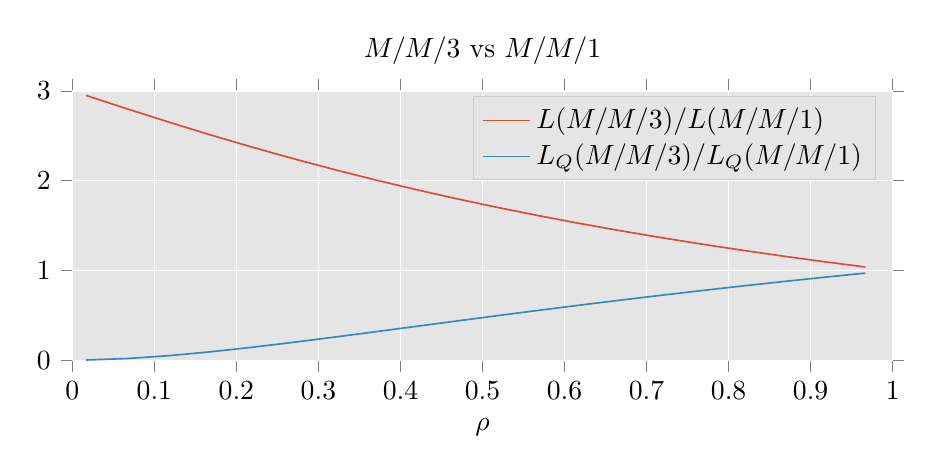
\begin{tikzpicture}

\definecolor{color1}{rgb}{0.203921568627451,0.541176470588235,0.741176470588235}
\definecolor{color0}{rgb}{0.886274509803922,0.290196078431373,0.2}

\begin{axis}[
title={$M/M/3$ vs $M/M/1$},
xlabel={$\rho$},
xmin=0, xmax=1,
ymin=0, ymax=3,
width=12cm,
height=5cm,
tick align=outside,
xmajorgrids,
x grid style={white},
ymajorgrids,
y grid style={white},
axis line style={white},
axis background/.style={fill=white!89.803921568627459!black},
legend cell align={left},
legend style={draw=white!80.0!black, fill=white!89.803921568627459!black},
legend entries={{$\E{L(M/M/3)}/\E{L(M/M/1)}$},{$\E{L_Q(M/M/3)}/\E{L_Q(M/M/1)}$}}
]
\addplot [semithick, color0]
table {%
0.0166666666666667 2.95002015316405
0.0666666666666667 2.80116959064328
0.116666666666667 2.65569956796278
0.166666666666667 2.51515151515152
0.216666666666667 2.38043779440288
0.266666666666667 2.2520325203252
0.316666666666667 2.13010978743284
0.366666666666667 2.01464254952627
0.416666666666667 1.90547263681592
0.466666666666667 1.8023598820059
0.516666666666667 1.7050162643383
0.566666666666667 1.61312938177183
0.616666666666667 1.52637836231238
0.666666666666667 1.44444444444444
0.716666666666667 1.36701781766159
0.766666666666667 1.2938018545632
0.816666666666667 1.22451553720904
0.866666666666667 1.15889464594128
0.916666666666667 1.09669211195929
0.966666666666667 1.03767781622453
};
\addplot [semithick, color1]
table {%
0.0166666666666667 0.00120918984280532
0.0666666666666667 0.0175438596491228
0.116666666666667 0.0488534396809571
0.166666666666667 0.0909090909090909
0.216666666666667 0.1404821280133
0.266666666666667 0.195121951219512
0.316666666666667 0.252978276103714
0.366666666666667 0.31266149870801
0.416666666666667 0.373134328358209
0.466666666666667 0.433628318584071
0.516666666666667 0.493579866461222
0.566666666666667 0.552581261950287
0.616666666666667 0.610343290236291
0.666666666666667 0.666666666666667
0.716666666666667 0.721420210690597
0.766666666666667 0.774524158125915
0.816666666666667 0.82593739250086
0.866666666666667 0.875647668393782
0.916666666666667 0.923664122137404
0.966666666666667 0.970011534025375
};
\end{axis}

\end{tikzpicture}
\caption{multi server versus single fast server}
  \label{fig:multisingle}
\end{figure}

The  code can be found on \texttt{github} in the \texttt{progs} directory.

\end{solution}
\end{question}


%%% Local Variables:
%%% mode: latex
%%% TeX-master: "book"
%%% End:

%  \section{Poisson Arrivals See Time Averages}
\label{sec:poisson-arrivals-see}

\subsection*{Theory and Exercises}

\Opensolutionfile{hint}
\Opensolutionfile{ans}

Suppose the following limit exists:
\begin{equation}\label{eq:jaap}
  \pi(n) 
= \lim_{m\to\infty} 
\frac1m\sum_{k=1}^m \1{L(A_k-) = n},
\end{equation}
where $\pi(n)$ is the long-run fraction of jobs that observe $n$
customers in the system at the moment of arrival.  It is natural to
ask whether $\pi(n)$ and $p(n)$, as defined by~\eqref{eq:p(n)}, are related, that is, whether what
customers see upon arrival is related to the time-average behavior of
the system. In this section we will derive the famous \recall{Poisson arrivals see time averages (PASTA)} condition  that ensures that  $\pi(n)=p(n)$. 


\begin{comment}
\begin{hint}
Check the definitions of $Y(0,t)$, $Y(1,t)$, $A(0,t)$ and so on. Make a drawing of $Y(0, t)$ and $Y(1,t)$ as functions of $t$. 
\end{hint}
  \begin{solution}
 $A(t)=\lfloor t\rfloor$ provided the unit of $t$ is in
  hours. $A(0,t)=A(t)$ and $A(n,t)=0$ for $n>0$.  Next, for $Y(0,t)$ we define, for notational ease, the fractional part of $t$ as $\{t\} = t - \lfloor t \rfloor$. Then,
  \begin{align*}
    Y(0,t)&= \frac 1{60} \lfloor t \rfloor + \{t\} \1{ \{t\} \in[59/60, 1)} \approx \frac{1}{60}t, \\
    Y(1,t)&= \frac{59}{60} \lfloor t \rfloor + \{t\} \1{\{t\}\in[0,59/60)} \approx \frac{59}{60}t. \\
\lambda(0) &= \lim_t \frac{A(0,t)}{Y(0,t)} = \lim_t \frac{t}{t/60} = 60, \\
\lambda(1) &= \lim_t \frac{A(1,t)}{Y(1,t)} = \lim_t\frac{0}{59/60 t} = 0 \\
\lambda(n) &= 0, \quad n\geq 1. \\
\lambda &= \lim_t \frac{A(t)}t  = 1 \\
p(0)  &= \frac{1}{60}, \\
p(1)  &= \frac{59}{60}, \\
\rho  &= \frac{59}{60}, \\
\pi(0)  &= 1. \\
  \end{align*}
  There is no queue so $\E{L_Q} = 0$, but $\E L = \rho$.  The queue
  length as observed by customers is equal to 0, because jobs only
  arrive when the server is free.
  \end{solution}
\end{exercise}
  \end{comment}

\begin{comment}
\begin{exercise}
 Consider another (theoretical) queueing system in which each
  customer requires precisely 1 minute. At the start of each hour, 59
  customers arrive. What is $p(n)$, what is $\pi(n)$? What is the time-average system length $\E{L}$?
  \begin{solution}
As in the previous problem, $\rho=59/60$.

For $p(n)$: the fraction of time the system contains $n=0$ jobs is $p(0)=1/60=1-\rho$. Also, as the service time of each job is precisely one minute, $p(n)=1/60$ for $n=1,\ldots, 59$. 

For $\pi(n)$, the first of the $59$ jobs sees a free server, thus $\pi(0)=1/59$. The second job of the $59$ jobs sees one job in system (and this job is in service), hence $\pi(1)=1/59$. More generally then, $\pi(n)=1/59$ for $n=0,\ldots 58$. 

Note in particular $p(59)=1/60 \neq \pi(59) = 0$. 

  Observe now that the average system length is very different from the
  previous example, even though $\rho = 59/60$ in both cases. Thus,
  knowledge of the load is not sufficient to make a statement about the
  average queue length.

  To compute the average queue length, as perceived by the customers,
  note that the first customer sees no queue, the second sees one
  customer in front, and so on. Thus, the average queue length as seen
  by customers is
  \begin{equation*}
   \frac{0+1+2+\cdots+58}{59}=\frac{1}{59}\frac{58\cdot 59}{2} = 29.
  \end{equation*}
The time average system length is $\E L = 59/60 + 58/60 + \cdots 1/60 + 0/60 = 59/2$. 
  \end{solution}
\end{exercise}
\end{comment}

We can make some progress by rewriting $\pi(n)$ in
the following way. Since $A(t)\to \infty$ as $t\to\infty$, it is reasonable 
that\footnote{See below for the proof.}
\begin{equation}\label{eq:132}
  \begin{split}
  \pi(n) &= \lim_{t\to\infty} \frac1{A(t)}\sum_{k=1}^{A(t)} \1{L(A_k-) = n} \\
  &= \lim_{t\to\infty} \frac1{A(t)}\sum_{k=1}^\infty \1{A_k \leq t, L(A_k-) = n} \\
  &= \lim_{t\to\infty} \frac{A(n,t)}{A(t)},
  \end{split}
\end{equation}
where we use~\eqref{eq:19} in the last row. But, 
\begin{equation}\label{eq:1333}
 \frac{A(n,t)}{t} 
= \frac{A(t)}t \frac{A(n,t)}{A(t)}
\to \lambda  \pi(n), \quad\text{as } t \to \infty, 
\end{equation}
where we use Eq.~\eqref{eq:3}, i.e., $A(t)/t \to \lambda$. 
Next, by  Eq.~\eqref{eq:21}, 
\begin{equation*}
\frac{A(n,t)}t = \frac{A(n,t)}{Y(n,t)}\frac{Y(n,t)}t \to \lambda(n) p(n), \quad\text{as } t \to \infty.
\end{equation*}
Thus
\begin{equation}\label{eq:13}
\lambda  \pi(n) = \lambda(n) p(n), 
\end{equation}
from which  follows our final result:
\begin{equation*}
  \lambda(n) = \lambda \iff \pi(n) = p(n), 
\end{equation*}

\begin{exercise}\label{ex:8} Show that for the case of Exercises~\ref{ex:111} and~\ref{ex:112}.  
$\pi(0)=1$, $\pi(n)=0$, for $n>0$.

\begin{solution}
  All arrivals see an empty system. Hence $A(0,t)/A(t) \approx (t/2)/(t/2) = 1$, and $A(n,t)=0$ for $n>0$. Thus, $\pi(0) = \lim_t A(0,t)/A(t) = 1$ and $\pi(n)=0$ for $n>0$. Recall from the other exercises that $p(0)=1/2$. Hence, time average statistics are not the same as statistics at arrival moments. 
\end{solution}

\end{exercise}

\begin{exercise}
  Check that~(\ref{eq:13})  holds for the system of Exercise~\ref{ex:8}
  \begin{solution}
From the relevant previous exercises, $\lambda = \lim_t A(t)/t = 1/2$. $\lambda(0)=1$, $p(0)=1/2$, and $\pi(0)=1$. Hence,
\begin{equation*}
  \lambda \pi(0) = \lambda(0) p(0) \implies  \frac 1 2 \times 1 = 1\times \frac 1 2.
\end{equation*}
For $n>0$ its easy, everything is 0.
  \end{solution}
\end{exercise}


So, why is this useful? Well, in words, it means that if the arrival
rate does not depend on the state of the system, i.e.,
$\lambda=\lambda(n)$, the sample average $\pi(n)$ is equal to the
time-average $p(n)$, i.e., $\pi(n)=p(n)$. But, when $\pi(n)=p(n)$, the
customer perception at arrival moments, i.e., $\pi(n)$, is the same as
the server perception, i.e., $p(n)$.

At the exercises above show, this property is not satisfied in
general.  However,  when the arrival process is
Poisson we have that $\lambda(n)=\lambda$. This fact is typically called \recall{PASTA:
  Poisson Arrivals See Time Averages}. Thus, when customers arrive in
accordance to a Poisson process (hence the inter-arrival times are
exponentially distributed), it must be that $\pi(n) = p(n)$, and
for the $M/M/1$ queue,
\begin{equation*}
  \pi(n) = p(n) = (1-\rho)\rho^n.
\end{equation*}


With the above reasoning, we can also establish a relation between
$\pi(n)$ and the statistics of the system as obtained by the
departures. For this we
turn again to Eq.~\eqref{eq:15}, i.e., $|A(n,t) - D(n,t)| \leq 1$. To
obtain Eq.~\eqref{eq:12} we divided both sides of this equation by the
time the system spends in a certain state. We can also use another
form:
\begin{equation*}
\frac{A(t)}t \frac{A(n,t)}{A(t)} = \frac{A(n,t)}t \approx \frac{D(n,t)}t 
= \frac{D(t)}t \frac{D(n,t)}{D(t)}.
\end{equation*}
Taking limits at the left and right, we see again that the left hand
becomes $\lambda \pi(n)$. For the right hand side, we use
Eq.~\eqref{eq:28} and define, analogous to \eqref{eq:132}, 
\begin{equation}
  \label{eq:33}
  \delta(n) = \lim_{t\to\infty} \frac{D(n,t)}{D(t)}.
\end{equation}
Thus, $\delta(n)$ is the long-run fraction of jobs that leave $n$ jobs
\emph{behind}. Clearly, then, if the limits exist, the right hand side
tends to $\delta \delta(n)$ as $t\to\infty$. Hence, for (queueing)
systems in which customers arrive and leave as single units, we have
\begin{equation}
  \label{eq:36}
  \lambda \pi(n) = \delta \delta(n).
\end{equation}
Moreover, if the system is rate-stable, i.e., the output rate $\delta$ is equal to the input rate $\lambda$, we obtain
\begin{equation}
  \label{eq:39}
\lambda = \delta \iff  \pi(n) = \delta(n).
\end{equation}
This means that the system as seen by arrivals, i.e., $\pi(n)$, is
the same as what jobs leave behind, i.e., $\delta(n)$.


\begin{exercise}
  When $\lambda\neq \delta$, is $\pi(n)\geq \delta(n)$?  
  \begin{hint}
Use that
    $\lambda \geq \delta$ always, and $\lambda=\delta$ when the system
    is rate-stable.
  \end{hint}
  \begin{solution}
    We have shown for one-step transition processes that
    $\lambda \pi(n) = \delta \delta(n)$. Thus,
    $\pi(n) = \delta(n)\delta /\lambda$. Since $\lambda\geq \delta$,
    we have that $\pi(n) \leq \delta(n)$.
  \end{solution}
\end{exercise}

\begin{exercise}
Show that 
\begin{equation*}
\lambda  \pi(n) = \lambda(n) p(n) = \mu(n+1) p(n+1) = \delta \delta(n).
\end{equation*}
What is the important condition for this to be true?
\begin{hint}
Check all definitions of $Y(n,t)/t$ and so on.
\end{hint}
\begin{solution}
  The important condition is that transitions occur as single
  steps. In other words, the relation is true for processes with
  \recall{one-step} transitions, i.e, when $|A(n,t) - D(n,t)|\leq 1$.
  In  that case, 
\begin{align*}
  \frac{A(n,t)}{t} &=   \frac{A(n,t)}{A(t)} \frac{A(t)}{t} \to \pi(n) \lambda\\
  \frac{A(n,t)}{t} &=   \frac{A(n,t)}{Y(n,t)} \frac{Y(n,t)}{t} \to \lambda(n)p(n)\\
  \frac{D(n,t)}{t} &=   \frac{D(n,t)}{Y(n+1,t)} \frac{Y(n+1,t)}{t} \to \mu(n+1)p(n+1)\\
  \frac{D(n,t)}{t} &=   \frac{D(n,t)}{D(t)} \frac{D(t)}{t} \to \delta(n)\delta \\
\end{align*}
\end{solution}
\end{exercise}



\begin{exercise}
  Why is $\mu(n) = \mu$ for the $M/M/1$ queue?  
  \begin{hint}
Think about the
    construction of the $M/M/1$ queue as a random walk, see
    Section~\ref{sec:queu-proc-as}.
  \end{hint}
 \begin{solution}
   The $M/M/1$-queue can be constructed as a reflection of the random
   walk $Z(t) = Z(0) + N_\lambda(t) - N_\mu(t)$. Clearly,
   downcrossings can only occur when $N_\mu$ fires. The rate at which
   the transitions of $N_\mu$ occur is constant, and, in particular,
   independent of the history of $Z$. 

   More specifically, for the interested, define
   $\sigma\{X(t) : t\in I\}$ as the $\sigma$-algebra generated by the
   stochastic procsses $\{X(t), t\in I\}$ on the index set $I$. Then,
   by construction of $\{N_\lambda(t)\}$ and $\{Z(t)\}$, we have that
   $\sigma\{Z(s) : s\in[0,t]\}$  and $\sigma\{N_\lambda(u) : u > t\}$ are independent.
 \end{solution}
\end{exercise}


\begin{exercise}
  Use the PASTA property and the ideas of Section~\ref{sec:level-cross-balance}
 to derive  for the $M/M/1$ queue that
$(\lambda + \mu) \pi(n) = \lambda \pi(n-1) + \mu \pi(n+1)$
  \begin{hint}
    Consider some state $n$ and count all transitions that `go in and
    out of' this state. Specifically, $A(n,t) + D(n-1,t)$ counts all
    transitions out of state $n$: $A(n,t)$ counts the number of
    arrivals that see $n$ in the system upon arrival, hence
    immediately after such arrivals the system contains $n+1$ jobs;
    likewise, $D(n-1,t)$ counts all jobs that leave $n-1$ jobs behind,
    hence immediately before such jobs depart the system contains $n$
    jobs.  In a similar way, $A(n-1,t) + D(n,t)$ counts all
    transitions into state $n$ (Recall once again, $D(n,t)$ counts the
    jobs that leave $n$ behind. Hence, when such departures occur,
    state $n$ is entered). Now use that `what goes in must go out'.    
  \end{hint}
  \begin{solution}
By  the hint,  the difference between the `in'
    transitions and the `out' transitions is at most 1 for all $t$. Thus,  we can write
    \begin{equation*}
      A(n,t) + D(n-1,t) \approx A(n-1,t) + D(n,t)
    \end{equation*}
From this, 
    \begin{equation*}
      \begin{split}
      A(n,t) + D(n-1,t) &\approx A(n-1,t) + D(n,t)  \iff \\
      \frac{A(n,t) + D(n-1,t)}t &\approx \frac{A(n-1,t) + D(n, t)}t \iff \\
      \frac{A(n,t)}t + \frac{D(n-1,t)}t &\approx \frac{A(n-1,t)}t + \frac{D(n,t)}t.
      \end{split}
    \end{equation*}
Using the ideas of Section~\ref{sec:level-cross-balance} this becomes for $t\to\infty$, 
\begin{equation*}
  (\lambda(n) +\mu(n))p(n) = \lambda(n-1)p(n-1) + \mu(n+1)p(n+1).
\end{equation*}
Since we are concerned here with the $M/M/1$ queue we have that
$ \lambda(n) = \lambda$ and $\mu(n) = \mu$, and using PASTA we have
that $p(n) = \pi(n)$. We are done.
  \end{solution}
\end{exercise}



There is a subtle problem in the transition from~\eqref{eq:jaap} to~\eqref{eq:132} and the derivation
of~\eqref{eq:1333}: $\pi(n)$ is defined as a limit over arrival epochs
while in $A(n,t)/t$ we take the limit over time. Now the observant
reader might ask why these limits should relate at all.  The
resolution lies in the \recall{renewal reward theorem}. This
theorem is very useful in its own right, and states  intuitively that 
when customers arrive at rate $\lambda$ and each customer pays an average amount $X$, then the system earns money at rate $Y=\lambda X$.  Figure~\ref{fig:renewal} provides graphical motivation about why this theorem is true; \citet{el-taha98:_sampl_path_analy_queuein_system}
gives  a (simple) proof.

\begin{theorem}[Renewal Reward Theorem, $Y=\lambda X$]
  Suppose the counting process $\{N(t), t\geq 0\}$ is such that
  $N(t)/t\to\lambda$ as $t\to\infty$, where $0<\lambda < \infty$. Let
  $\{Y(t), t\geq 0\}$ be a non-decreasing right-continuous
  (deterministic) process. Define $X_k = Y(T_k)-Y(T_{k-1})$,
  $k\geq 1$, where $T_k$ are the epochs at which $N$ increases, i.e.,
  $N(t) = \{k : T_k \leq t\}$. Then $Y(t)/t$ has a limit iff
  $n^{-1}\sum_k^n X_k$ has a limit in which case $Y=\lambda X$, i.e.,
  \begin{equation*}
  \lim_t \frac{Y(t)}t=Y \iff \lim_n \frac 1n\sum_k^n X_k =X \implies Y=\lambda X.
  \end{equation*}
\end{theorem}

\begin{figure}[ht]
  \centering
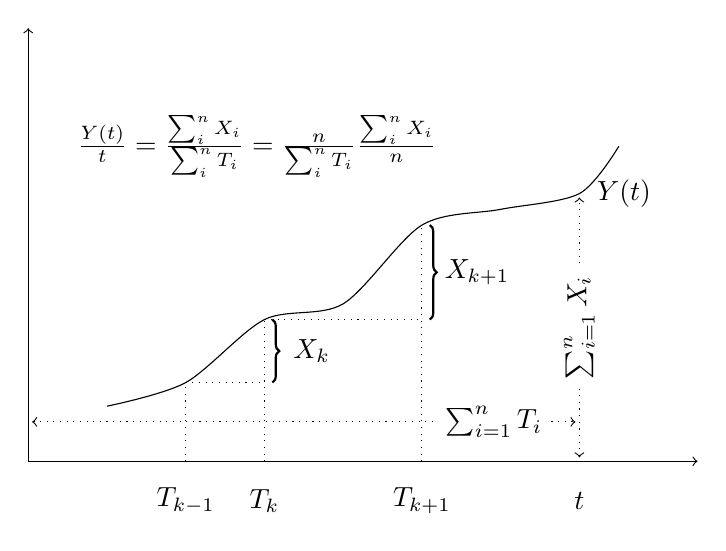
\begin{tikzpicture}[scale=1]
%axis
\draw[->] (0,0) -- coordinate (x axis mid) (8.5,0);
\draw[->] (0,0) -- coordinate (y axis mid) (0,5.5);
%\node[below=0.2cm] at (x axis mid) {$t$};

\draw plot [smooth] coordinates {(1,0.7) (2,1) (3,1.8) (4,2) (5,3) (6,3.2) (7, 3.4) (7.5,4.0)};
\node[right]  at (7.1,3.4) {$Y(t)$};
\node  at (7.,-0.5) {$t$};

\node  at (2.,-0.5) {$T_{k-1}$};
\draw[dotted] (2,0)--(2,1);
\draw[dotted] (2,1)--(3,1);


\node  at (3.,-0.5) {$T_{k}$};
\draw[dotted] (3,0)--(3,1.8);
\draw[dotted] (3,1.8)--(5,1.8);

\draw [
    thick,
    decoration={brace, mirror, raise=0.1cm },
    decorate
] (3,1) -- (3,1.8)
node[pos=0.5, xshift=0.6cm]  {$X_k$}; 


\node  at (5.,-0.5) {$T_{k+1}$};
\draw[dotted] (5,0)--(5,3);

\draw [
    thick,
    decoration={brace, mirror, raise=0.1cm },
    decorate
] (5,1.8) -- (5,3)
node[pos=0.5, xshift=0.7cm]  {$X_{k+1}$}; 

\node[right] at (0.5,4) {$\frac{Y(t)}t = \frac{\sum_i^n X_i}{\sum_{i}^n T_i} = \frac{n}{\sum_{i}^n T_i} \frac{\sum_i^n X_i}n $};


\draw[dotted,<->, =stealth] (7,0.05)--(7,3.35) node[midway, rotate=90, fill=white] {$\sum_{i=1}^n X_i$};
\draw[dotted,<->, =stealth] (0.05,0.5)--(6.95,0.5) node[pos=0.85, fill=white] {$\sum_{i=1}^n T_i$};
\end{tikzpicture}
\caption{A graphical `proof' of $Y=\lambda X$. Here $Y(t)/t\to Y$, $n/\sum^n_i T_i\to \lambda$ and $n^{-1}\sum_i^n X_i \to X$.  (Observe that in the
  figure $X_k$ does not represent an interarrival time; instead it
  corresponds to the increment of (the graph of) $Y(t)$ between two
  consecutive epochs $T_{k-1}$ and $T_k$ at which $Y(t)$ is
  observed.) }
  \label{fig:renewal}
\end{figure}


\begin{exercise}
Use the renewal reward theorem to show that~(\ref{eq:132}) is valid.
\begin{hint}
Check that the conditions of the renewal reward theorem are satisfied in the above proof~\eqref{eq:1333}. Then define  
\begin{align*}
  Y(t) &:= A(n,t) = \sum_{k=1}^{A(t)} \1{L(A_k-) = n} \\
X_k &:= Y(A_k) - Y(A_{k-1}) = A(n, A_k) - A(n, A_{k-1}) = \1{L(A_k-)=n}.
\end{align*}

\end{hint}
\begin{solution}
First we check the conditions.  The counting process here is $\{A(t)\}$ and the epochs at which
    $A(t)$ increases are $\{A_k\}$. By assumption, $A_k\to\infty$,
    hence $A(t)\to\infty$ as $t\to\infty$. Moreover, by assumption
    $A(t)/t \to \lambda$. Also $A(n,t)$ is evidently non-decreasing and
    $A(n,t)\to\infty$ as $t\to\infty$.


From the definitions in the hint,   
\begin{equation*}
X= \lim_{m\to\infty} \frac 1 m \sum_{k=1}^m X_k =\lim_{m\to\infty} \frac 1 m \sum_{k=1}^m \1{L(A_k-)=n} = \pi(n).
\end{equation*}
Since $Y=\lim_t Y(t)/t = \lim_t A(n,t)/t$ it follows from the renewal reward theorem that
\begin{equation*}
  Y=\lambda X \implies \lim_t \frac{A(n,t)} t = \lambda X = \lambda \pi(n).
\end{equation*}
Thus, Eq.~\eqref{eq:1333} follows from the renewal reward theorem.
\end{solution}
\end{exercise}





\Closesolutionfile{hint}
\Closesolutionfile{ans}

\opt{solutionfiles}{
\subsection*{Hints}
\input{hint}
\subsection*{Solutions}
\input{ans}
}
\clearpage

%%% Local Variables:
%%% mode: latex
%%% TeX-master: "../book"
%%% End:

%  \section{Little's Law}
\label{sec:littles-law}


There is an important relation between the average time $\E W$ a job
spends in the system and the long-run time-average number $\E L$ of jobs
that is contained in the system. This is Little's law:
\begin{equation}
  \E L = \lambda \E W.
\end{equation}
Here we provide a sketch of the proof, c.f.,
\cite{el-taha98:_sampl_path_analy_queuein_system} for the details. In
the forthcoming sections we will apply Little's law often. Part of the
usefulness of Little's law is that it applies to all input-output
systems, whether it is a queueing system or an inventory system or
some much more general system.

We start with defining a few intuitively useful concepts.  Clearly, from~\eqref{eq:11}, 
\begin{equation*}
  \mathscr{L}(t) = \frac 1 t\int_0^t L(s)\, \d s =  \frac 1 t\int_0^t (A(s)-D(s)) \, \d s
\end{equation*}
is the time-average of the number of jobs in the system during
$[0,t]$. Observe once again from the second equation that
$\int_0^t L(s)\,\d s$ is the area enclosed between the graphs of $A(s)$
and $D(s)$.


The waiting time of the $k$th job is the time between the moment the
job arrives and departs, that is
\begin{equation*}
  W_k = \int_0^\infty \1{A_k \leq s < D_k}\,\d s.
\end{equation*}

We can actually relate $W_k$ to $ \mathscr{L}(t)$, see
Figure~\ref{fig:atltdt}. Consider a departure time $T$ at which the
system is empty. Observe that $A(T) = D(T)$, as at time $T$ all jobs
that arrived up to $T$ also have left. Thus, for all jobs $k\leq A(T)$
we have that $D_k \leq A(T)$, so that we can replace the integration
bounds in the above expression for $W_k$ by
\begin{equation*}
  W_k = \int_0^T \1{A_k \leq s < D_k}\,\d s.
\end{equation*}
Moreover, if $s\leq T$,
\begin{equation*}
L(s) = \sum_{k=1}^\infty \1{A_k \leq s < D_k} = \sum_{k=1}^{A(T)}\1{A_k \leq s < D_k}.
\end{equation*}
Therefore,
\begin{equation*}
  \begin{split}
  \int_0^T L(s)\, \d s & = \int_0^T \sum_{k=1}^{A(T)} 1\{A_k \leq s < D_k\} \, \d s \\
& =  \sum_{k=1}^{A(T)}\int_0^T  1\{A_k \leq s < D_k\} \, \d s =  \sum_{k=1}^{A(T)} W_k.
  \end{split}
\end{equation*}
Thus, in words, the area between the graphs of $A(s)$ and $D(s)$ must
be equal to the total waiting time spent by all jobs in the system
until $T$. 
From this, 
\begin{equation*}
  \mathscr{L}(T) = \frac 1 T  \int_0^T L(s)\, \d s  = \frac{A(T)} T \frac{1}{A(T)} \sum_{k=1}^{A(T)} W_k.
\end{equation*}
Finally, assuming there are an infinite number of times
$0\leq T_i<T_{i+1}<\cdots$, $T_i\to\infty$, at which $A(T_i) = D(T_i)$
and the following limits exist
\begin{align*}
 \mathscr{L}(T_i) &\to \E L,&
\frac{A(T_i)}{T_i} &\to \lambda, &
\frac{1}{A(T_i)} \sum_{k=1}^{A(T_i)} W_k &\to \E W,
\end{align*}
we obtain \recall{Little's law}
\begin{equation*}
\E L = \lambda \E W.
\end{equation*}

As a useful first application, consider a server of the $G/G/1$ queue
as a system by itself. Assume the system is rate-stable, for otherwise
the above limits do not exists.  The arrival rate at the server is
$\lambda$ and the time a job remains in at the server is $\E S$.
Thus, the averate number of jobs at the server is
$\E{L_S} = \lambda \E S$. As $\lambda \E{S} = \rho$, we get
$\E{L_S} = \rho$.

\begin{remark}
  Sometimes (often?) students memorize Little's law in the wrong
  way. Thus, as an easy check, use the dimensions of the concepts:
  $\E L$ is an average \emph{number}, $\lambda$ is a \emph{rate},
  i.e., \emph{numbers per unit time}, and $\E W$ is waiting
  \emph{time}. \recall{Checking the dimensions} in the formula
  prevents painfull mistakes.

  Note also that $\E L\neq L(t)$; to clarify, the expected number of
  items in the system is not necessarily equal to the number of items
  in the system at some arbitrary time $t$. Thus, Little's law need
  not hold at all moments in time; it is a statement about
  \emph{averages}.
\end{remark}

\paragraph{Summary}

Perhaps a summary of the most useful results and concepts of the previous sections
are in order here:
\begin{itemize}
\item Arrival rate,  departure  rate, rate stability:  $\lambda = \gamma$
\item PASTA: $\lambda \pi(n) = \lambda(n) p(n)$,
\item Recursions $\lambda(n)p(n) = \mu(n+1) p(n+1)$,
\item Renewal reward: $Y=\lambda X$
\item Little's law: $\E L =\lambda \E W$.
\end{itemize}
\recall{Memorize these results.} We will use them often in the sequel,
but in other courses these results will also prove very useful.


\begin{question}
  For a given single server queueing system the average number of
  customers in the system is $\E L = 10$, customers arrive at rate
  $\lambda=5$ per hour and are served at rate $\mu=6$ per hour.
  \begin{enumerate}
  \item What is the average time customers spend in the system?
  \item Suppose at the moment you join the system, the number of
    customers in the system is 10. What is your expected time in the
    system? 
  \item Why are the answers between these two questions different?
  \end{enumerate}
  \hint{ Think about the data that is given in either situation. Check
    the units when applying Little's law.}

    \begin{solution}
      \begin{enumerate}
      \item This was my initial answer (which is wrong):
        `$\E W = \lambda \E L = \lambda 10$'.  Interestingly, I typed
        in Little's law in the wrong way\ldots So, be aware! It's all
        too easy to make mistakes with Little's law.

    This is correct: 
    \begin{equation*}
      \E W = \E L/\lambda = 10/\lambda = 10/5 = 2
    \end{equation*}
    and \emph{not} $\E W = 10/\mu=10/6=5/3$ hour.
  \item The time you spend in the system is the expected remaining
    service time $\E{S_r}$, i.e., the time to serve the customer in
    service at the moment of arrival, plus $9/\mu$, i.e., the time to
    clear the queue of 9 customers (recall, 1 job is in service.)
  \item In the second question, it is \emph{given} that the system
    length is 10 at the moment of arrival. Now, $L$ as `seen' by a
    given customer upon arrival need not be the same as the
    time-average $L$.
  \end{enumerate}
    \end{solution}
\end{question}

\begin{question}
 Which assumptions did we use to prove Little's law?
  \begin{solution}
    \begin{itemize}
    \item 
 $A(t)/t \to \lambda$ as $t\to \infty$, i.e., $A(t)/t$ has a limit as $t$ converges to $\infty$. 
  \item There exists a sequence of points $T_k, k=0,1,2,\ldots$ in time such that the server is idle. 
  \item Either of the limits $\sum_k^n W_k/n = \sum_k^n S_k /n $ or
    $t^{-1}\int_0^t L(s) \d s$ exists, in which case the other exists.
    \end{itemize}
  \end{solution}
\end{question}


\begin{question}
  Provide a graphical interpration of the proof of Little's law.
  \hint{ Make a drawing of $A(t)$ and $D(t)$ until time $T$, i.e., the
    first time the system is empty.}
  \begin{solution}
    The area enclosed between the graphs of $A(t)$ and $D(t)$ until
    $T$ can be `chopped up' in two ways: in the horizontal direction
    and the vertical direction. (Please make the drawing as you go
    along\ldots) A horizontal line between $A(t)$ and $D(t)$
    corresponds to the waiting time of a job, while a vertical line
    corresponds to the number of jobs in the system at time $t$. Now
    adding all horizontal lines (by integrating along the $y$-axis)
    makes up the total amount of waiting done by all the jobs until
    time $T$. On the other hand, adding the vertical lines (by
    integrating along the $x$-axis) is equal to the summation of all
    jobs in the system. Since the area is the same no matter whether
    you sum it in the horizontal or vertical direction:
    \begin{equation*}
      \sum_{k=1}^{A(T)}  W_k = \text{eclosed area} = \int_0^T (A(t)-D(t))\,dt. 
    \end{equation*}
 Dividing both sides by $A(T)$ gives
    \begin{equation*}
\frac{1}{A(T)} \sum_{k=1}^{A(T)}  W_k =\frac{1}{A(T)} \int_0^T (A(t)-D(t))\,dt. 
    \end{equation*}

    Finally, observe that this equality holds between any two times
    $T_i, T_{i+1}$, where times $\{T_i\}$ are such that
    $A(T_i)=D(T_i)$. Then, as $T_i\to \infty$ which we assumed from
    the on-set, $\frac{1}{A(T_i)} \sum_{k=1}^{A(T_i)} W_k\to \E W$,
    and
    \begin{equation*}
\frac{T_i}{A(T_i)}\frac{1}{T_i} \int_0^{T_i} (A(t)-D(t))\,dt \to \lambda^{-1} \E L.
    \end{equation*}
Hence, Little's law follows.
  \end{solution}
\end{question}


\begin{question}\nvf{You can skip this exercise. I moved it from the G/G/1 section to here.}
  Discuss the results of Figure~\ref{fig:multisingle} in terms of
  waiting time ratios. Recall, in this figure we compare queue and
  system length, not waiting times.

  \begin{solution}
    By Little's law, the ratio between the waiting times is the same.

The processing capacity of $c$ servers that work at rate 1 is equal to
one server that works at rate $c$. The, intuitive, difference between
the $M/M/c$ queue and the $M/M/1$ queue with a fast server is that
jobs spend shorter time in queue in the $M/M/c$ case---jobs can be
served in parallel, hence do not always have to wait in queue for
server capacity---, but spend longer time in service---simply because
the servers in the $M/M/c$ case works at rate $1$, not at rate $c$.

\end{solution}
\end{question}



%%% Local Variables:
%%% mode: latex
%%% TeX-master: "book"
%%% End:

%  \section{Some Useful Identities}
\label{sec:some-usef-ident}


\subsection*{Theory and Exercises}

\Opensolutionfile{hint}
\Opensolutionfile{ans}
With the PASTA property and Little's law we can derive a number of
useful and simple results for the $M/G/1$ queue by which we can analyze a large number of practical queueing situations, see Exercise~\ref{exer: Hall} and below. In particular, we concentrate here on server utilization, i.e., $\rho$, and average queue length and waiting times. Recall, to use the
PASTA, we need to assume that jobs arrive as a Poisson process.

The fraction of time the server is empty is $1-\rho = p(0)$. By PASTA,
$\pi(0)=p(0)$, hence the fraction of customers that enter an empty
system is also $1-\rho$. Similarly, the fraction of customers that find the server occupied at arrival is equal to the the utilization $\rho$. 



Suppose that at $A_k$, i.e., the arrival epoch of the $k$th job, the
server is busy.  The \recall{remaining service time} $S_{r,k}$ as seen by job
$k$ is the time between $A_k$ and the departure epoch of the job in
service. If the server is free at $A_k$, we set $S_{r,k}=0$.  Define
the average \recall{remaining service time} as seen at arrival epochs as
\begin{equation*}
  \E{S_r} = \lim_{n\to\infty} \frac1n \sum_{k=1}^n S_{r,k},
\end{equation*}
provided this limit exists. 

\begin{exercise}
  It is an easy mistake to think that $\E{S_r} = \E S$ when service
  times are exponential. Why is this wrong?
  \begin{hint}
Realize again that $\E{S_r}$ includes the jobs that arrive at an empty system.
  \end{hint}
  \begin{solution}
    $\E{S_r \given S_r>0} = \E S$ for the $M/M/1$ queue, and
    $\E{S_r} = \rho \E{S_r \given S_r>0}$ for the $M/G/1$ queue, it
    follows that
  \begin{equation*}
 \E{S_r} = \rho \E{S_r\given S_r>0} = \rho \E S.
  \end{equation*}
  \end{solution}
\end{exercise}

\begin{exercise}($M/G/1$)
Use  the PASTA property to show that 
\begin{equation}\label{eq:37}
\E{S_r} =  \rho \E{S_r\given S_r>0}.
\end{equation}
\begin{hint}
By the PASTA property, a fraction~$\rho$ of the arrivals sees the server occupied, while a fraction $1-\rho$ sees
a free server.  
\end{hint}
\begin{solution}
\begin{equation*}
\E{S_r} =   \rho \E{S_r\given S_r >0} + (1-\rho)\cdot \E{S_r\given S_r = 0} = \rho \E{S_r\given S_r>0},
\end{equation*}
since, evidently, $\E{S_r\given S_r=0}=0$.  
\end{solution}
\end{exercise}

\begin{exercise}
  What would you guess for $\E{S_r\given S_r>0}$ for the $M/D/1$ queue? 
  \begin{solution}
    Since the service times are deterministic (and constant), I would
    guess that on average half of the service time remains at the
    moment a job arrives. If the service time is $D$ always, then
    $\E{S_r\given S_r>0} = \lambda D/2$.  
  \end{solution}
\end{exercise}

\begin{exercise}
  Try to derive relation~(\ref{eq:37}) with sample path
  arguments. 
  \begin{hint}
This requires some extra definitions, similar to
  $A(n,t)$ as defined in~\eqref{eq:19}.
  \end{hint}
  \begin{solution}
    This is, admittedly, not simple, so let us work in stages. Define
    $A(+,t)$ as the number of arrivals that see a job in service. As
    the server is only busy at time $t$ when $L(t)>0$, we define
    \begin{equation*}
      A(+,t) = \sum_{k=1}^\infty \1{A_k\leq t}\1{L(A_k) > 0}.
    \end{equation*}
    Next, define $\tilde D_k = \min\{D_i: D_i \geq A_k\}$ as the first
    departure after the arrival time $A_k$ of job $k$. We need to
    consider two cases. If $\tilde D_k = D_k$ then, obviously, the
    first departure after $A_k$ coincides with the departure time of
    job $k$. This is only possible if $L(A_k) = 0$. But then, it must
    be that the remaining service time of the job in service at time
    $A_k$ is 0, as there is no job in service. Otherwise, if
    $L(A_k)>0$ it must be that $\tilde D_k < D_k$, and, as a
    consequence, the remaining service time of the job in service at
    time $A_k$ is equal to $\tilde D_k - A_k$. All in all, the total
    amount of remaining service times added up for all arrivals up to
    time $t$ can be written as
    \begin{equation*}
      S_r(t) = \sum_{k=1}^\infty (\tilde D_k - A_k) \1{A_k \leq t, L(A_k) > 0}.
    \end{equation*}
    The remaining service time averaged over all arrivals up to
    time $t$ is therefore $S_r(t)/A(t)$. We can now rewrite this to
\begin{equation*}
  \frac{S_r(t)}{A(t)} = 
  \frac{A(+,t)}{A(t)} \frac{S_r(t)}{A(+,t)}, 
\end{equation*}
and interpret these fractions.  First, consider
\begin{equation*}
  \frac{A(+,t)}{A(t)} = 
\frac{\sum_{k=1}^\infty \1{A_k\leq t, L(A_k) > 0}}{\sum_{k=1}^\infty \1{A_k\leq t}}.
\end{equation*}
This is the number of jobs up to time $t$ that see at least one job in
the system divided by the total number of arrivals up to time $t$. Thus, as $t\to\infty$, 
\begin{equation*}
  \frac{A(+,t)}{A(t)} \to \sum_{n=1}^\infty \pi(n) = 1-\pi(0).
\end{equation*}
With PASTA we can conclude that $1-\pi(0) = 1-p(0)= \rho$. Second,
\begin{equation*}
\frac{S_r(t)}{A(+,t)} 
= \frac{\sum_{k=1}^\infty (\tilde D_k - A_k) \1{A_k\leq t, L(A_k) > 0}}{\sum_{k=1}^\infty \1{A_k\leq t, L(A_k)>0}},
\end{equation*}
is the total amount of remaining service time up to time $t$ divided by
the number of arrivals up to time $t$ that see at least one job in the system. Thus, 
if the limit exists, we can \emph{define}
\begin{equation*}
\E{S_r \given S_r>0}  =\lim_{t\to\infty} \frac{S_r(t)}{A(+,t)}.
\end{equation*}
  \end{solution}
\end{exercise}

Next, consider the waiting time in queue.  
\begin{exercise}($M/G/1$)
Show  that the expected time in queue is
\begin{equation}\label{eq:24}
  \E{W_Q} = \E{S_r} + \E{L_Q} \E S.
\end{equation}
\begin{hint}
  What happens when you enter a queue? First you have to wait until the job in service (if there is any) completes, and then you have to wait for the queue to clear.
\end{hint}
\begin{solution}
It is evident that the expected waiting time for an arriving customer is the expected
remaining service time plus the expected time in queue. The expected
time in queue  must be equal to the expected number of
customers in queue at an arrival epoch times the expected service time
per customer, assuming that service times are i.i.d. If the arrival
process is Poisson, it follows from PASTA that the average number of
jobs in queue perceived by arriving customers is also the
\emph{time-average} number of jobs in queue~$\E{L_Q}$.  
\end{solution}
\end{exercise}
 
\begin{exercise}($M/G/1$)
  Use the previous problem and Little's law to derive that 
\begin{equation}\label{eq:35}
  \E{W_Q} = \frac{\E{S_r}}{1-\rho} = \frac{\rho}{1-\rho} \E{S_r\given S_r>0}.
\end{equation}
\begin{hint}
Use Little's law to see that $\E{L_Q} = \lambda \E{W_Q}$. Substitute this in~(\ref{eq:24}) and simplify.
\end{hint}
\begin{solution}
With  Little's law $\E{L_Q} = \lambda \E{W_Q}$. Using this,
\begin{equation*}
  \E{W_Q} = \E{S_r} + \lambda \E{W_Q} \E S  =\E{S_r} + \rho \E{W_Q},
\end{equation*}
since $\rho=\lambda \E S$. But this gives for the $M/G/1$ queue that
\begin{equation*}
  \E{W_Q} = \frac{\E{S_r}}{1-\rho} = \frac{\rho}{1-\rho} \E{S_r\given S_r>0},
\end{equation*}
where we use~(\ref{eq:37}) in the last equation.
\end{solution}
\end{exercise}

The average waiting time $\E W$ in the entire system, i.e., in queue
plus in service, becomes
\begin{equation*}
  \E W = \E{W_Q}+ \E S = \frac{\E{S_r}}{1-\rho} + \E S.
\end{equation*}

The situation can be significantly simplified for the $M/M/1$ queue as
then the service times are also exponential, hence memoryless,
implying that $\E{S_r\given S_r>0} = \E S$. 

\begin{exercise}($M/M/1$) Derive that
\begin{equation}\label{eq:ew}
  \E W = \frac{\E S}{1-\rho}.
\end{equation}
\begin{solution}
Using~(\ref{eq:37}),
\begin{equation*}
  \begin{split}
  \E W 
&= \E{W_Q}+ \E S = 
\frac{\E{S_r}}{1-\rho} + \E S \\
&= \frac{\rho \E S}{1-\rho} + \E S = \frac{\E S}{1-\rho}.
  \end{split}
\end{equation*}
\end{solution}
\end{exercise}

\begin{exercise}($M/M/1$) Use the PASTA property to conclude that
\begin{equation}\label{eq:61}
  \E W = \E L  \E S + \E S,
\end{equation}
and apply Little's law to find~(\ref{eq:ew}). 
\begin{hint}
Another way to derive the above result is to conclude from PASTA that
the expected number of jobs in the system at an arrival is $\E{L}$.
Since all these jobs require an expected service time $\E S$,
including the job in service by the memory-less property, the time in
queue is $\E L \E S$. The time in the system is then the waiting time
plus the service time. Next, use Little's law $\E L = \lambda \E W$.
\end{hint}
\begin{solution}
From the hint
\begin{equation}
  \E W = \E L  \E S + \E S = \lambda \E W \E S + \E S = \rho \E W  + \E S.
\end{equation}
Substituting Little's law $\E L = \lambda \E W$ and simplifying,
\begin{equation*}
\E W = \frac{\E S}{1-\rho}.
\end{equation*}
\end{solution}
\end{exercise}


\begin{exercise}
  Why is Eq.~(\ref{eq:61}) not true in general for the $M/G/1$ queue?
  \begin{hint}
Think about the consequences of memoryless service times.
  \end{hint}
  \begin{solution}
    Because the remaining service time of the job in service, provided
    there is a job in the system upon arrival, is not exponentially
    distributed in general. Only for the $M/M/1$ queue the service
    times are exponentially distributed, hence memoryless. And only
    when the service time is memoryless, the service time after an
    interruption is still exponential.
  \end{solution}
\end{exercise}

\begin{exercise}($M/M/1$)
Show that 
\begin{equation}\label{eq:wqes}
  \E{W_Q} = \E L \E S = \frac{\rho^2}{1-\rho} \frac 1 \lambda,
\end{equation}
  \begin{solution}
\begin{equation}
  \E{W_Q} = \E L \E S = \lambda \E W \E S= \rho \E W = \frac{\rho}{1-\rho} \E S = \frac{\rho^2}{1-\rho} \frac 1 \lambda,
\end{equation}
which is consistent with our earlier result.  
  \end{solution}
\end{exercise}

Finally, we find expressions for  the average lengths.
\begin{exercise}($M/M/1$)
  Show that
  \begin{align*}
\E L &= \frac\rho{1-\rho}, & \E{L_Q} &= \frac{\rho^2}{1-\rho}, & \E{L_s} &= \rho.
  \end{align*}
  \begin{hint}
    Apply Little's law to the $\E{L_Q}$ and so on, and use the earlier expressions for $\E{W_Q}$ and so on.
  \end{hint}
  \begin{solution}
With Little's law, 
\begin{equation*}
  \begin{split}
\E L &= \lambda \E W = \frac{\lambda \E S}{1-\rho} = \frac\rho{1-\rho}, \\
  \E{L_Q} &= \lambda \E{W_Q} = \frac{\rho^2}{1-\rho}, \\
  \E{L_s} &= \E L - \E{L_Q} = \frac{\rho}{1-\rho} - \frac{\rho^2}{1-\rho} = \rho, 
      \end{split}
\end{equation*}
since, the expected number of jobs in service $\E{L_s}$ is
equal to the expected number of busy servers.
  \end{solution}
\end{exercise}

\begin{exercise}($M/M/1$) Explain that
$\E{L_Q} = \sum_{n=1}^\infty (n-1)\pi(n)$, and  use this to find that $\E{L_Q}=\rho^2/(1-\rho)$.
  \begin{solution}
    The fraction of time the system contains $n$ jobs is $\pi(n)$ (by
    PASTA). When the system contains $n>0$ jobs, the number in queue
    is one less, i.e., $n-1$.

    \begin{equation*}
      \begin{split}
\E{L_Q} 
&= \sum_{n=1}^\infty (n-1)\pi(n) 
= (1-\rho)\sum_{n=1}^\infty (n-1) \rho^n\\
&= \rho (1-\rho)\sum_{n=1}^\infty (n-1) \rho^{n-1}
= \rho \sum_{n=1}^\infty (n-1) \pi(n-1)\\
&= \rho \sum_{n=0}^\infty n \pi(n)
= \rho \frac{\rho}{1-\rho}.
      \end{split}
    \end{equation*}

Another way to get the same result is by splitting: 
\begin{equation*}
  \begin{split}
\E{L_Q} 
&= \sum_{n=1}^\infty (n-1)\pi(n) 
=\sum_{n=1}^\infty n\pi(n) -\sum_{n=1}^\infty \pi(n)\\
&= \E L - (1-\pi(0)) = \E L - \rho.
  \end{split}
\end{equation*}
  \end{solution}
\end{exercise}

\begin{comment}
\begin{exercise}[use=false]
  As a challenge you can try to derive \eqref{eq:24} by means of sample path arguments.
  \begin{solution}
    \TBD
  \end{solution}
\end{exercise}
\end{comment}




\begin{exercise}($M/M/1$)
  Use the PASTA property to see that the expected waiting time in the
  system must also be equal to
  $\E W = \sum_{n=0}^\infty \E{W_Q \given N=n} \pi(n) + \E S$, 
where $\E{W_Q \given N=n}$ is the waiting time in queue given that an
arrival sees $N=n$ customers upon arrival. Then, 
 motivate that $\E{W_Q \given N=1} = \E S$. Finally, combine the above to see that 
$\E W = \E S \sum_{n=0}^\infty n \pi(n) + \E S = \E S \E L + \E S$.
  \begin{solution}
    \begin{enumerate}
    \item The time in the system $\E W$ is the sum of the time in
      queue plus the service time of the job itself.  Conditioning on
      the number of jobs $N$ in the system at arrival moments, i.e.,
      conditioning on $\pi(n)$, gives the result.  
    \item $\E{W_Q\given N=0}=0$, of course. If $N=1$, there must be a job
      in service.  Because of the memoryless property of the service
      times, the remaining service time of the customer in service is
      still exponentially distributed with mean $\E S$. Thus,
      $\E{W_Q\given N=1}=\E S$. 
    \item The expected service time for a customer still in queue is
      $\E S$.  Therefore, for each $n$ we have that, when service
      times are exponential, $\E{W_Q\given N=n}= n \E S$. The probability
      to see $n$ jobs in the system by an arrival is $\pi(n)$ which,
      by PASTA, is equal to $p(n)$. Since $\E L = \sum_n n p(n)$, the
      result follows.
    \end{enumerate}
  \end{solution}
\end{exercise}

\begin{comment}
  
\begin{exercise}[use=false] Note: the question is unclear, and needs more explanation. 

  There is distinction between $\E{L_Q}$, i.e., the time-average queue
  length, and the expected number of jobs in the system given that the
  server is busy, i.e., $\E{L\given B}$.  is $\E{L_Q} \neq \E{L\given B}$?
\begin{solution}
  $\E{L_Q}$ is the time average of the queue length process (in steady
  state). Hence, $\E{L_Q}$ contains also the time the queue is
  empty. $\E{L\given B}$ the other hand, is the time average of the
  queue length process, provided the server is busy. Even though the
  queue may be empty while the server is busy, the fraction of time
  the queue length is zero given that the server is busy, is smaller
  than the fraction of time the queue length is zero.  Hence,
  $\E{L\given B} > \E{L_Q}$.
\end{solution}
\end{exercise}
\end{comment}

\begin{exercise}($M/G/1$)
Show that the variance of the number of jobs in the system $L$ is
$\V L = \rho/(1-\rho)^2.$
  \begin{hint}
    $\V{L} = \E{L^2} - (\E L)^2$. We already know $\E L$ so it remains
    to compute $\E{L^2}$. Then, $\E{L^2 }= \sum_{n=0}^\infty n^2 \pi(n)$. Use that $\pi(n)=\rho^n(1-\rho)$ is the probability to see $n$ jobs in the system. Now simplify.    
  \end{hint}
  \begin{solution}
The starting point is  $\V{L} = \E{L^2} - (\E L)^2$. 

With wolfram alpha we get
    \begin{equation*}
      \begin{split}
      \E{L^2 }
&= \sum_{n=0}^\infty n^2 \pi(n) \\
&= \rho \frac{1+\rho}{(1-\rho)^2}.
      \end{split}
    \end{equation*}
    Thus,
\begin{equation*}
\V L = \frac{\rho(1+\rho)}{(1-\rho)^2}-\frac{\rho^2}{(1-\rho)^2} = \frac{\rho}{(1-\rho)^2}.
\end{equation*}


Lets see whether I can get the result for $\E{L^2}$ by myself.  One way
is to use the standard formula for a geometric series with $\rho < 1$:
\begin{equation*}
\dfrac{1}{1-\rho} = \sum_{n=0}^{\infty}\rho^n.
\end{equation*}
If we differentiate the left and right hand side with respect to
$\rho$  and then  multiply with $\rho$ we obtain
\begin{equation*}
\dfrac{\rho}{(1-\rho)^2}=\sum_{n=0}^{\infty}n\rho^n.
\end{equation*}
Again, differentiating and multiplying with $\rho$ yields, 
\begin{equation*}
  \begin{split}
\rho \frac{(1-\rho)^2 + \rho2(1-\rho)}{(1-\rho)^4} 
&= \rho \frac{1-2\rho+\rho^2 + 2\rho-2\rho^2}{(1-\rho)^4} \\
&= \rho \frac{(1-\rho)^2}{(1-\rho)^4} \\
&=\rho \dfrac{1+\rho}{(1-\rho)^3}\\
&=\sum_{n=0}^{\infty}n^2\rho^n
  \end{split}
\end{equation*}
and hence
\begin{equation*}
(1-\rho)\sum_{n=0}^{\infty}n^2\rho^n = \rho\dfrac{1+\rho}{(1-\rho)^2}
\end{equation*}
% Write
% $\partial_\rho$ as a shorthand for the derivative with respect to
% $\rho$. Then observe that
% $(\rho \partial_\rho) \rho^n = \rho n \rho^{n-1} = n\rho^n$, hence
% $(\rho \partial_\rho)^2 \rho^n =
% (\rho \partial_\rho)(\rho\partial_\rho) \rho^n = (\rho \partial
% \rho) n \rho^n = n^2\rho^n$. With this,
% \begin{equation*}
%   \begin{split}
% (1-\rho)  \sum_{n=0}^\infty n^2 \rho^n 
% &=  (1-\rho)(\rho \partial_\rho)^2   \sum_{n=0}^\infty \rho^n\\
% &=  (1-\rho)(\rho \partial_\rho)^2   \frac1{1-\rho}\\
% &=  (1-\rho)\rho \partial_\rho   \frac\rho{(1-\rho)^2}\\
% &=  (1-\rho) \rho  \frac{1+\rho}{(1-\rho)^3} \\
% &=  \rho  \frac{1+\rho}{(1-\rho)^2}.
%   \end{split}
% \end{equation*}
Observe that here we just compute the second moment of a geometric
random variable.


Another way to derive the result is by noting that
$\sum_{i=1}^n i= n(n+1)/2$ from which we get that
$n^2 = -n + 2\sum_{i=1}^n i$. Substituting this relation into
$\sum_n n^2 \rho^n$ leads to
\begin{equation*}
  \begin{split}
    \sum_{n=0}^\infty n^2 \rho^n 
&=    \sum_{n=0}^\infty \left(\sum_{i=1}^\infty 2i \1{i\leq n}  - n\right)\rho^n 
=    \sum_{n=0}^\infty \sum_{i=0}^\infty 2i\1{i\leq n}\rho^n  - \sum_{n=0}^\infty n\rho^n \\
&=    \sum_{i=0}^\infty 2i \sum_{n=i}^\infty \rho^n  - \frac{\E L}{1-\rho} 
=    \sum_{i=0}^\infty 2i \rho^i \sum_{n=0}^\infty \rho^n  - \frac{\E L}{1-\rho} \\
&=    \frac2{1-\rho} \sum_{i=0}^\infty i \rho^i   - \frac{\E L}{1-\rho} 
=    \frac2{(1-\rho)^2} \E L - \frac{\E L}{1-\rho} \\
&=    \frac{\E L}{1-\rho}  \left(\frac2{1-\rho}  - 1\right) 
=    \frac{\E L}{1-\rho}  \frac{1+\rho}{1-\rho} \\
&=    \frac{\rho}{1-\rho}  \frac{1+\rho}{(1-\rho)^2}.
\end{split}
\end{equation*}

A last method is based on $z$-transforms:
\begin{equation*}
  \phi(z) = \E{z^L} = \sum_{n=0}^\infty z^n p(n) = (1-\rho) \sum_{n=0}^\infty (\rho z)^n = \frac{1-\rho}{1-\rho z}.
\end{equation*}
Then 
\begin{equation*}
  \E L = \left.\frac d {dz} \phi(z)\right|_{z=1} = \frac{\rho}{1-\rho},
\end{equation*}
and 
\begin{equation*}
  \E{L(L-1)}= \left.\phi''(z)\right|_{z=1} = \frac{2\rho^2}{(1-\rho)^2}.
\end{equation*}
Thus,
\begin{equation*}
\E L^2 =   \E{L(L-1)} + \E L.
\end{equation*}
Hence,
\begin{equation*}
  \begin{split}
\E L^2 
&=   \frac{2\rho^2}{(1-\rho)^2} + \frac\rho{1-\rho} \\
&=   \frac{2\rho^2}{(1-\rho)^2} + \frac\rho(1-\rho){(1-\rho)2} \\
&=   \frac{\rho^2+\rho}{(1-\rho)^2} = \rho \frac{1+\rho}{(1-\rho)^2}.
  \end{split}
\end{equation*}

A bit of algebra gives the previous results.
  \end{solution}
\end{exercise}


\begin{exercise}$(M/M/1$) 
To see how large the variance of $L$ is, relative to the mean number of jobs
in the system, we typically consider the square coefficient of
variation (SCV). Show that the square coefficient of variation of $L$ is $1/\rho$. What do you conclude from this?
\begin{hint}
  SCV  $=\V X/(\E X)^2$. 
\end{hint}
  \begin{solution}
To see how large this variance is, relative to the mean number of jobs
in the system, we typically consider the square coefficient of
variation (SCV). As $\E L = \rho/(1-\rho)$,
\begin{equation*}
  \frac{\V L}{(\E{L})^2} = \frac 1 \rho.
\end{equation*}
Thus, the SCV becomes smaller as $\rho$ increases, but does not become
lower than $1$. So, realizing that the SCV of the exponential
distribution is 1, the distribution of the number of jobs in the
system has larger relative variability than the exponential
distribution.
  \end{solution}
\end{exercise}

\begin{comment}
\begin{exercise}
Consider an $M/M/2$ queueing system that is very heavily utilized, with an arrival rate of 11 customers per hour, and a  service rate of 6 customers per hour per server.
 Determine $\E{L_Q}$ and $\E{W_Q}$. Compare your solution to an $M/M/1$ queue with $\rho=11/12$. Why are your answers similar or different?
  \begin{solution}

Here are the results for the $M/M/2$ queue.

\begin{pyconsole}
labda = 11.
mu = 6
c = 2

rho = labda/mu
rho < c  # is the system stable?
\end{pyconsole}

Compute $L_s$ and so on


\begin{pyconsole}
from math import factorial

G = sum(rho**n/factorial(n) for n in range(c))
G += rho**c/factorial(c)/(1.-rho/c)
P0 = 1./G
P0

Lq = rho**(c+1)/c/(factorial(c)*(1.-rho/c)**2)*P0
Lq
Lq/labda # Wq

Ls = Lq + rho
Ls
Ls/labda # Ws

ES = 1./mu # expected service time
ES
\end{pyconsole}

Now consider the $M/M/1$ queue with twice the service rate, i.e., now we take $\mu = 6c = 12$. 

\begin{pyconsole}
mu = c*6

rho = labda/mu

P0 = 1-rho
P0

Lq = rho**2/(1.-rho)
Lq
Lq/labda # Wq

Ls = rho/(1.-rho)
Ls
Ls/labda # Ws

ES = 1./mu # expected service time
ES
\end{pyconsole}
    \end{solution}
\end{exercise}
\end{comment}




\begin{exercise}(Hall 5.2) \label{exer: Hall} After observing a single server queue for
  several days, the following steady-state probabilities have been
  determined: $p(0)=0.4$, $p(1) = 0.3$, $p(2)=0.2$, $p(3)=0.05$ and
  $p(4)=0.05$. The arrival rate is 10 customers per hour. 
  \begin{enumerate}
  \item Determine $\E L$ and  $\E{L_Q}$. 
  \item Using Little's formula, determine $\E W$ and $\E{W_Q}$. 
\item Determine $\V{L}$ and $\V{L_Q}$.
  \item Determine the service time and the utilization.
  \end{enumerate}
    \begin{solution}
      \begin{enumerate}
      \item 
      When a problem is mainly of a computational type, I coded the
      solutions and show you all the numerical answers. Thus, please
      read the code too since this shows the precise steps by which I
      obtain the answer. (The code is typically nearly identical to
      the mathematical formulas; you should not have any difficulty
      understanding the code.) I also show many intermediate numerical
      results so that you can check each step in your computations. (In
      the computations below I typically use the simplest, but often
      not the most efficient, code.)

\begin{pyconsole}
P = [0.4, 0.3, 0.2, 0.05, 0.05]
L = sum(n*P[n] for n in range(len(P)))
L
\end{pyconsole}

There can only be a queue when a job is in service. Since there is
$m=1$ server, we subtract $m$ from the amount of jobs in the system.
Before we do this, we need to ensure that $n-m$ does not become
negative. Thus, $\E{L_Q} = \sum_n \max\{n-m, 0\} p(n)$.

\begin{pyconsole}
m = 1
Lq = sum(max(n-m,0)*P[n] for n in range(len(P)))
Lq
\end{pyconsole}

\item 

\begin{pyconsole}
labda = 10./60
Wq = Lq/labda # in minutes
Wq
Wq/60 # in hours

W = L/labda # in minutes
W
W/60 # in hours
\end{pyconsole}

\item 

\begin{pyconsole}
from math import sqrt
var_L = sum((n-L)**2*P[n] for n in range(len(P)))
var_L
sqrt(var_L)
\end{pyconsole}


\begin{pyconsole}
var_Lq = sum((max(n-m,0)-Lq)**2*P[n] for n in range(len(P)))
var_Lq
sqrt(var_Lq)
\end{pyconsole}

\item 

\begin{pyconsole}
mu = 1./(W-Wq)
1./mu # in minutes

rho = labda/mu
rho
\end{pyconsole}

\begin{pyconsole}
rho = L-Lq
rho
\end{pyconsole}
This checks the previous line.

The utilization must also by equal to the fraction of time the server is busy. 
\begin{pyconsole}
u = 1 - P[0]
u
\end{pyconsole}

Yet another way: Suppose we have $m$ servers. If the system is empty,
all $m$ servers are idle. If the system contains one customer, $m-1$
servers are idle. Therefore, in general, the average fraction of time
the server is idle is
\begin{equation*}
1- u = \sum_{n=0}^\infty \max\{n-m, 0\}  p_n,
\end{equation*}
as in case there are more than $m$ customers in the system, the
number of idle servers is $0$.


\begin{pyconsole}
idle = sum( max(m-n,0)*P[n] for n in range(len(P)))
idle
\end{pyconsole}

  \end{enumerate}
   \end{solution}
 
\end{exercise}

\begin{exercise}
  (Hall 5.5) An $M/M/1$ queue has an arrival rate of 100 per hour and
  a service rate of 140 per hour.
 What is $p(n)$?  What are $\E{L_Q}$, $\E L$ 
\begin{solution}
  \begin{enumerate}
  \item 
$p(n) = (1-\rho)\rho^n$

\item 

\begin{pyconsole}
labda = 100. # per hour
mu = 140. # per hour
ES = 1./mu
rho = labda/mu
rho 
1-rho

L = rho/(1.-rho)
L
Lq = rho**2/(1.-rho)
Lq

W = 1./(1.-rho) * ES
W
Wq = rho/(1.-rho) * ES
Wq
\end{pyconsole}
  \end{enumerate}
  \end{solution}
\end{exercise}

\begin{exercise}(Hall, 5.6)
  An $M/M/1$ queue has been found to have an average waiting time in queue of 1 minute. The arrival rate is known to be 5 customers per minute.
 What are the service rate and utilization? Calculate $\E{L_Q}$,  $\E L$ and $\E W$. Finally, 
 The queue operator would like to provide chairs for waiting customers. He would like to have a sufficient number so that all customers can sit down at least 90 percent of the time. How many chairs should he provide?
    \begin{solution}
      \begin{enumerate}
      \item $\E{W_Q} = \frac{1}{\lambda}\frac{\rho^2}{1-\rho}$. Since
        $\E{W_Q}$ and $\lambda$ is given we can use this formula to
        solve for $\rho$ with the abc-formula (and using that
        $\rho > 0$):

\begin{pyconsole}
labda = 5. # per minute
Wq = 1.
a = 1.
b = labda*Wq
c = -labda*Wq
rho = (-b + sqrt(b*b-4*a*c))/(2*a)
rho 

ES = rho/labda
ES
\end{pyconsole} 

\item 

\begin{pyconsole}
Lq = labda*Wq
Lq

W = Wq + ES
W

L = labda*W
L
\end{pyconsole} 

\item 

The problem is to find $n$ such that
      $\sum_{j=0}^n p_j > 0.9$.

\begin{pyconsole} 
total = 0. 
j = 0
while total <= 0.9:
   total += (1-rho)*rho**j
   j += 1

total
j
n = j- 1 # the number of chairs 
\end{pyconsole} 

Observe that $j$ is one too high once the condition is satisfied, thus subtract one.

As a check, I use that $(1-\rho) \sum_{j=0}^n \rho^j = 1-\rho^{n+1}$.

\begin{pyconsole}
1-rho**(n) #  this must be too small.
1-rho**(n+1) # this must be OK.
\end{pyconsole} 

And indeed, we found the right $n$.

  \end{enumerate}
    \end{solution}
\end{exercise}

\begin{exercise}
  (Hall 5.7). A single server queueing system is known to have Poisson
  arrivals and exponential service times. However, the arrival rate
  and service time are state dependent. As the queue becomes longer,
  servers work faster, and the arrival rate declines, yielding the
  following functions (all in units of number per hour):
  $\lambda(0) = 5$, $\lambda(1)=3$, $\lambda(2)=2$,
  $\lambda(n)=0, n\geq 3$, $\mu(0) = 0$, $\mu(1)=2$, $\mu(2)=3$, $\mu(n)=4, n\geq 3$. 
Calculate the state probabilities, i.e., $p(n)$ for $n=0,\ldots$. 
\begin{hint}
Use the level-crossing equations of the $M(n)/M(n)/1$ queue.
\end{hint}
    \begin{solution}
      Follows right away from the hint.
    \end{solution}
\end{exercise}

\begin{exercise}
  (Hall 5.14) An airline phone reservation line has one server and a
  buffer for two customers. The arrival rate 6 customers per hour, and
  a service rate of just 5 customers per hour. Arrivals are Poisson and service times are exponential. 
 Estimate $\E{L_Q}$ and the average number of customers served per hour. Then, estimate $\E{L_Q}$ for a buffer of size 5. What is the impact of the increased buffer size on the number of customers served per hour?
  \begin{hint}
This is a queueing system with loss, in particular the $M/M/1/1+2$ queue.
  \end{hint}
    \begin{solution}
      \begin{enumerate}
      \item 
First compute $\E{L_Q}$ for the case with a buffer for $2$ customers.

\begin{pyconsole}
labda = 6.
mu = 5.
rho = labda/mu
c = 1
b = 2
\end{pyconsole} 

Set $p(n) = \rho^n$ initially, and normalize later. Use the
expressions for the $M(n)/M(n)/1$ queue.  Observe that $\rho>1$. Since
the size of the system is $c+b+1$ is finite, all formulas work for
this case too.


There are 4 states in total: $0,1,2,3$. (The reason to import numpy here and convert the lists to arrays is to fix the output precision to 3, otherwise we get long floats in the output.)

\begin{pyconsole}
import numpy as np
np.set_printoptions(precision=3)

P = np.array([rho**n for n in range(c+b+1)])
P

G = sum(P)
G

P /= G # normalize
P
\end{pyconsole} 

\begin{pyconsole}
L = sum(n*P[n] for n in range(len(P)))
L

Lq = sum((n-c)*P[n] for n in range(c,len(P)))
Lq
\end{pyconsole} 


The number of jobs served per hour must be equal to the number of jobs
accepted, i.e., not lost. The fraction of customers lost is equal to
the fraction of customers that sees a full system.

\begin{pyconsole}
lost = labda*P[-1] # the last element of P
lost

accepted = labda*(1.-P[-1]) # rate at which jobs are accepted
accepted
\end{pyconsole}  

\item 
Now increase the buffer $b$ to 5.

\begin{pyconsole}
b = 5
P = np.array([rho**n for n in range(c+b+1)])
P
G = sum(P)
G

P /= G # normalize
P

L = sum(n*P[n] for n in range(len(P)))
L

accepted = labda*(1.-P[-1])
accepted
\end{pyconsole}      
  \end{enumerate}
    \end{solution}
\end{exercise}

\begin{comment}
\begin{exercise}[use=false]
  The code is in \texttt{progs/mm1\_waiting\_time_distribution.py}. In
  mm1\_waiting\_time_distribution.py we compute the waiting time
  distribution. At this point in the text this distribution has not
  yet been derived.  This problem should be moved to another section.

Consider an $M/M/1$ queue with $\mu=1.2$ per hour. Make plots of the
waiting time distribution $\P{W_Q\leq t}$ for various values of
$\lambda$ to show the dependency on the arrival rate. Compare this to
the dependence of average waiting time $\E{W_Q}$ on $\lambda$.

The idea of making such plots is to analyze
  whether the service capacity suffices for a situation in which one
  doesn't know the arrival rate very accurately, but one can control
  the service rate, e.g., by hiring personnel.
  \begin{solution}
    Let's just plot the waiting time distribution
for various values of $\lambda$. 


\begin{figure}[ht]
  \centering
\includegraphics{progs/mm1_waiting_time.tex}
  \caption{The waiting time distribution for various values of the arrival rate.}
  \label{fig:waitingtime}
\end{figure}


\end{solution}

\end{exercise}
\end{comment}


\begin{exercise}(Hall 5.3) After observing a queue with two servers
  for several days, the following steady-state probabilities have been
  determined: $p(0)=0.4$, $p(1) = 0.3$, $p(2)=0.2$, $p(3)=0.05$ and
  $p(4)=0.05$. The arrival rate is 10 customers per hour.
  \begin{enumerate}
  \item Determine $\E L$ and  $\E{L_Q}$. 
  \item Using Little's formula, determine $\E W$ and $\E{W_Q}$. 
  \item Determine $\V L$ and $\V{L_Q}$.
  \item Determine the service time and the utilization.
  \end{enumerate}
  \begin{solution}
    \begin{enumerate}
    \item Determine $\E L$ and  $\E{L_Q}$. 

\begin{pyconsole}
P = [0.4, 0.3, 0.2, 0.05, 0.05]

c = 2
Lq = sum((n-c)*P[n] for n in range(c,len(P)))
Lq

L= sum(n*P[n] for n in range(len(P)))
L
\end{pyconsole}

\item Using Little's formula, determine $\E W$ and $\E{W_Q}$. 
\begin{pyconsole}
labda = 10./60
Wq = Lq/labda # in minutes
Wq
Wq/60 # in hours

W = L/labda
W
\end{pyconsole} 

\item Determine $\V L$ and $\V{L_Q}$.
\begin{pyconsole}
from math import sqrt
var_L = sum((n-L)**2*P[n] for n in range(len(P)))
var_L
sqrt(var_L)
\end{pyconsole} 

\item Determine the service time and the utilization.
\begin{pyconsole}
var_q = sum((max(n-c,0)-Lq)**2*P[n] for n in range(len(P)))
var_q
sqrt(var_q)
\end{pyconsole}

  \end{enumerate}
    \end{solution}
\end{exercise}  

\begin{exercise}
  (Hall 5.8) The queueing system at a fast-food stand behaves in a
  peculiar fashion. When there is no one in the queue, people are
  reluctant to use the stand, fearing that the food is
  unsavory. People are also reluctant to use the stand when the queue
  is long. This yields the following arrival rates (in numbers per hour): $\lambda(0) = 10$, $\lambda(1)=15$, $\lambda(2)=15$, $\lambda(3)=10$, $\lambda(4)=5$, $\lambda(n)=0, n\geq 5$. The stand has two servers, each of which can operate at 5 per hour. Service times are exponential, and the arrival process is Poisson.
 Calculate the steady state probabilities. Next,  what is the average arrival rate? Finally,
 Determine $\E L$, $\E{L_Q}$, $\E W$ and $\E{W_Q}$.
  \begin{solution}
First the service rates.
\begin{pyconsole}
import numpy as np
labda = [10., 15., 15., 10., 5.]
c = 2
mn = 2*np.ones(len(labda)+1, dtype=int)  # number of active servers
mn[0] = 0  # no service if system is empty
mn[1] = 1  # one busy server if just one job present
mu = 5*mn # service rate is 5 times no of active servers
mu
\end{pyconsole}

Since there can be arrivals in states $0,\ldots, 4$,  the system can contain $0$ to $5$ customers, i.e., $p(0),\ldots, p(5)$.

Use the level crossing result for the $M(n)/M(n)/1$ queue:

\begin{pyconsole}
P = [1]*(len(labda)+1)
for i in range(1,len(P)):
    P[i] = labda[i-1]/mu[i]*P[i-1]

P = np.array(P) # unnormalized probabilities
P
\end{pyconsole}

\begin{pyconsole}
G = sum(P) # normalization constant
G
P /= G # normalize
P 
\end{pyconsole} 

$\lambda = \sum_{n}\lambda(n) p(n)$.

\begin{pyconsole}
labdaBar = sum(labda[n]*P[n] for n in range(len(labda)))
labdaBar
\end{pyconsole}


The average number in the system is: 

\begin{pyconsole}
Ls = sum(n*P[n] for n in range(len(P)))
Ls
\end{pyconsole}


The average number in queue 
\begin{pyconsole}
c = 2
Lq = sum((n-c)*P[n] for n in range(c,len(P)))
Lq
\end{pyconsole} 

And now the waiting times:

\begin{pyconsole}
Ws = Ls/labdaBar
Ws # time in the system

Wq = Lq/labdaBar
Wq # time in queue
\end{pyconsole} 

    \end{solution}
\end{exercise}

\begin{exercise}
  (Hall 5.10) A repair/maintenance facility would like to determine
  how many employees should be working in its tool crib. The service
  time is exponential, with mean 4 minutes, and customers arrive by a
  Poisson process with rate 28 per hour. The customers are actually
  maintenance workers at the facility, and are compensated at the same
  rate as the tool crib employees.
 What is $\E W$ for $c=1, 2, 3$, or $4$ servers? How many employees should work in the tool crib?
  \begin{hint}
Realize that we have to control the number of servers. Hence,
    we are dealing with a multi-server queue, i.e., the $M/M/c$
    queue. Use the formulas of Eq.~\eqref{eq:9}.

The remark that maintenance workers are compensated at the same rate
as the tool crib workers confused me a bit at first.  Some thought
revealed that the consequence of this remark is that is it just as
expensive to let the tool crib workers wait (to help maintenance
workers) as to let the maintenance workers wait for tools. (Recall, in
queueing systems always somebody has to wait, either the customer in queue or
the server being idle. If it is very expensive to let customers wait, the number
of servers must be high, whereas if servers are relatively expensive, customers have to do the waiting.)
  \end{hint}
  \begin{solution}
    \begin{enumerate}
    \item 
      Would one server/person do? 
\begin{pyconsole}
labda = 28./60 # arrivals per minute
ES = 4.
labda*ES
\end{pyconsole} 

If $c=1$, the load $\rho=\lambda \E S/c >1$ is clearly undesirable for one server.  We need at
least two servers.

It is not relevant to focus on the time in the system , as time
  in service needs to be spent anyway. Hence, we focus on the waiting
  time in queue.


I just convert the formulas of~\eqref{eq:9} to python code. This saves
me time during the computations.

\begin{pyconsole}
def WQ(c, labda, ES):
    rho = labda*ES/c
    G = sum([(c*rho)**n/factorial(n) for n in range(c)])
    G += (c*rho)**c/(1.-rho)/factorial(c)
    Lq = (c*rho)**c/(factorial(c)*G) * rho/(1.-rho)**2
    return Lq/labda # Wq, Little's law

\end{pyconsole} 

Considering the scenario with one server is superfluous as $\rho>1$ in
that case.

What is the waiting time for $c=2$ servers?

\begin{pyconsole}
WQ(2, 28./60, 4) # in minutes
WQ(2, 28./60, 4)/60. # in hours
\end{pyconsole}

What is the waiting time for $c=3$ servers?

\begin{pyconsole}
WQ(3, 28./60, 4)   # in minutes
WQ(3, 28./60, 4)/60. # in hours
\end{pyconsole}


What is the waiting time for $c=4$ servers?

\begin{pyconsole}
WQ(4, 28./60, 4) # in minutes
WQ(4, 28./60, 4)/60. # in hours
\end{pyconsole} 

In the next  part of the question we will interpret these numbers.

\item 
Since both types of workers cost the same amount of money per unit
time, it is best to divide the amount of waiting/idleness equally over
both types of workers.  I am inclined to reason as follows. The
average amount of waiting time done by the maintenance workers per
hour is $\lambda \E{W_Q}$. To see this, note that maintenance workers arrive at rate $\lambda$, and each worker waits on average $\E{W_Q}$ minutes. Thus, worker time is wasted at rate $\lambda \E{W_Q}$. Intestingly, with Little's lawy, $\E{L_Q}=\lambda \E{W_Q}$, i.e., the rate at which workers waste capacity (i.e.  waiting in queue) is $\E{L_Q}$. On the other hand, the  rate of work capacity wasted by the tool crib employees being idle is $c-\lambda \E{S}$, as $\lambda \E S$ is the average number of servers busy, while $c$ crib servers are available.

As both types of
employees are equally expensive, we need to choose $c$ such that
the number of maintenance workers waiting (i.e., being idle because they are waiting in queue), is  equal to the number of crib workers being idle. In other words, we search for a $c$ such that $\E{L_Q} \approx c- \lambda \E S$ (where, of course, $\E{L_Q}$ depends on $c$.)


\begin{pyconsole}
labda = 28./60
ES = 4.
c = 2
ELQ = labda*WQ(c, labda, ES)
ELQ
c-labda*ES
\end{pyconsole} 
Now the maintenance employees wait more than the tool crib employees.

\begin{pyconsole}
c = 3
ELQ = labda*WQ(c, labda, ES)
ELQ
c-labda*ES
\end{pyconsole} 

\begin{pyconsole}
c = 4
ELQ = labda*WQ(c, labda, ES)
ELQ
c-labda*ES
\end{pyconsole} 

Clearly, $c=3$ should do.
  \end{enumerate}
    \end{solution}
\end{exercise}






\Closesolutionfile{hint}
\Closesolutionfile{ans}
\subsection*{Hints}
\input{hint}
\subsection*{Solutions}
\input{ans}
\clearpage

%%% Local Variables:
%%% mode: latex
%%% TeX-master: t
%%% End:

%  \section
[$M^X/M/1$ Queue: Expected Waiting Time]
{$\mathbf{M^X/M/1}$ Queue: Expected Waiting Time}
\label{sec:mxm1-queue:-expected}

\subsection*{Theory and Exercises}
\label{sec:exercises}

\Opensolutionfile{hint}
\Opensolutionfile{ans}

It is not always the case that jobs arrive in single units, they can
also arrive as batches. For instance, cars and busses arrive at a fast
food restaurant so that the batch size consists of the number of
people in the vehicle.  In this section we derive a formula to compute
the expected queue length for this queueing process. 


Assume that jobs arrive as a Poisson process with rate $\lambda$ and
each \emph{job} contains multiple \emph{items}.  Let $A_k$ be the
arrival time of job $k$ and $A(t)$ the number of job arrivals up to
time $t$. Denote by $B_k$ the number of items that job $k$ brings into
the system.  We assume that $\{B_k\}$ is an i.i.d. sequence of
discrete random variables distributed as a generic random variable $B$
such that $\P{B = k} = f(k)$, where $f(k)$ is a given set of
probabilities. We write
\begin{equation*}
  G(k) = \P{B>k} = \sum_{m=k+1}^\infty f(m),
\end{equation*}
for the \emph{survivor function} of $B$.  We also assume that the
service time of each item is exponentially distributed with average
$1/\mu$. Thus, the average time to serve a job is
$\E{B}\E{S}=\E B/\mu$. This queueing situation denoted by the shorthand
$M^X/M/1$.

The first criterion we must check for the $M^X/M/1$ queue is the
stability: the service rate must be larger than the arrival rate of
work. To determine the latter, the total number of items $N(t)$
arrived up to time $t$ must be equal to the number of arrivals $A(t)$
up to time $t$ times the batch size of each arrival, i.e.,
\begin{equation*}
N(t)=  \sum_{k=1}^\infty B_k \1{A_k \leq t} = \sum_{k=1}^{A(t)} B_k.
\end{equation*}
The (stochastic) process $\{N(t)\}$ is known as the \recall{compound
  Poisson process}. Clearly, the rate at which items arrive is
approximately
\begin{equation*}
  \frac{N(t)}t = \frac{A(t)}t \frac1{A(t)}\sum_{i=k}^{A(t)} B_k.
\end{equation*}
As in  the limit $A(t)/t \to \lambda$ and $(A(t))^{-1}\sum_{k=1}^{A(t)} B_k \to \E{B}$, we see that
\begin{align*}
\frac{N(t)}t \to \lambda \E B.
\end{align*}
Thus, for stability, it is necessary that the service rate
$\mu=1/\E S$ for items is larger than the rate at which items
arrive. Hence we require that the load is such that
\begin{equation*}
\rho = \lambda \E B \E S = \frac{\lambda \E B} \mu < 1.
\end{equation*}

For the average waiting time, we can use the derivation of
$\E{W_Q}=\E{S_r}/(1-\rho)$ of Section~\ref{sec:some-usef-ident} for
inspiration. Suppose a batch finds $\E{L}$ items in the system upon
arrival. By the memoryless property of the service distribution, the
expected remaining service time of the item in service (if any) is
$\E S$. Therefore the expected time the entire batch, i.e., the job,
spends in queue is
\begin{equation*}
  \E{W_{Q,b}} = \E{L} \E S;
\end{equation*}
compare Eq.~\ref{eq:wqes}. Note that this is not the same as
$\E{W_Q}$, which is the expected time an \emph{item} spends in queue.
If $B_r$ is the number of items of the batch currently in service
($B_r=0$ if the server is idle), and $L_{Q,b}$ the number of batches
in queue, then
\begin{equation*}
  \E{L} = \E{L_{Q,b}}\E B + \E{B_r}.
\end{equation*}
With  Little's law, $\E{L_{Q,b}} = \lambda \E{W_{Q,b}}$, hence
\begin{equation*}
  \E{W_{Q,b}} = \lambda \E S \E B \E{W_{Q,b}} + \E S \E{B_r} = \rho \E{W_{Q,b}} + \E S \E{B_r},
\end{equation*}
hence,
\begin{equation*}
  \E{W_{Q,b}} = \frac{\E S}{1-\rho}\E{B_r}.
\end{equation*}
And then, from the first equation, 
\begin{equation*}
  \E{L} = \frac{\E{W_{Q,b}}}{\E S} = \frac{\E{B_r}}{1-\rho}.
\end{equation*}
Below we prove that 
\begin{equation}\label{eq:br}
  \E{B_r} = \rho\frac{\E{B^2}}{2\E B} + \frac\rho2.
\end{equation}
In an exercise below we rewrite this to
\begin{equation}\label{eq:43}
\E{L}  = \frac{\E{B_r}}{1-\rho} = \frac{1+C_s^2}2 \frac{\rho}{1-\rho} \E B + \frac12\frac\rho{1-\rho},
\end{equation}
where
\begin{equation*}
C_s^2 = \frac{\V B}{(\E B)^2},
\end{equation*}
is the square coefficient of variation of the batch sizes.  Observe
that this is nearly the same as $M/G/1$ waiting time
formula~\ref{eq:710}, a result we derive in Section~\ref{sec:mg1}. 

Thus, to compute the average number of items in the system, we only
need to know the first and second moment (or the variance) of the
batch size $B$. Thus, no matter how `complicated' the distribution of
$B$, when its second moment exists, the average queue length and
waiting time can be computed with the above result. 



\begin{figure}[t]
  \centering
  \begin{tikzpicture}[scale=0.8,
  open/.style={shape=circle, fill=white, inner sep=1pt, draw, node contents=},
  closed/.style={shape=circle, fill=black, inner sep=1pt, draw, node contents=}]

    % y = zero line
    \draw (-0.5, 0) -- (18.5, 0); 
    % level crossing
    \draw (-0.5, 2.5) -- (18.5, 2.5) 
    node[pos=0.65, fill=white, above]  {$\sum_{k=1}^n \1{B_k \geq i}$}
    node[pos=0.92, fill=white]  {$y=i$};


    \draw node (c1) at (0,3.5) [closed, label={}]
          node (c2) at (3.5,0)[open, label={}]
     (c1) to (c2);
    \draw[dotted] (0,0) -- (0,3.5) node[midway, fill=white] {$B_1$};
    \draw[dotted, <->] (1, 0.05) -- (1, 2.45) node[fill=white, midway, rotate=90] {$i$};


    \draw node (c1) at (3.5,1.5) [closed, label={}]
          node (c2) at (5,0)[open, label={}]
     (c1) to (c2);
    \draw[dotted] (3.5,0.1) -- (3.5,1.5) node[midway, fill=white] {$B_2$};

    \draw node (c1) at (5,4) [closed, label={}]
          node (c2) at (9,0)[open, label={}]
     (c1) to (c2);
    \draw[dotted] (5,0.1) -- (5,4) node[midway, fill=white] {$B_3$};
    \draw[dotted, <->] (6.5, 0.05) -- (6.5, 2.45) node[fill=white, midway, rotate=90] {$i$};

    \draw node (c1) at (9,2.3) [closed, label={}]
          node (c2) at (11.3,0)[open, label={}]
     (c1) to (c2);
    \draw[dotted] (9,0.1) -- (9,2.3) node[midway, fill=white] {$B_4$};

    % end
    \draw node (c1) at (14.5,3.5) [closed, label={}]
          node (c2) at (18,0)[open, label={}]
     (c1) to (c2);
    \draw[dotted] (14.5,0.1) -- (14.5,3.5) node[midway, fill=white ] {$B_n$};
    \draw[dotted, <->] (15.5, 0.05) -- (15.5, 2.45) node[fill=white, midway, rotate=90] {$i$};
    

    % bottom line
    \draw[<->] (0, -0.6) -- (18, -.6) node[fill=white, midway] {$\sum_{k=1}^n B_k$};
\end{tikzpicture}

\caption{The remaining job size as a function of time. A batch crosses
  the line $y=i$ iff it contains an $i$th item. Thus, the number of
  $i$th items in $n$ batches is $\sum_{k=1}^n \1{B_k\geq i}$. The
  total number of items arrived is $\sum_k^n B_k$. The fraction of
  time an $i$th item is in service is therefore
  $\sum_k^n \1{B_k\geq i}/\sum_k^n B_k$.}
  \label{fig:remainingservicetime}
\end{figure}


We now turn to proving~\eqref{eq:br} with sample-path arguments and
counting; it is an elegant line of reasoning. First concentrate on the
time the server is busy, i.e., just remove all idle times, and plot
the remaining job size during the service of the job, c.f,
Figure~\ref{fig:remainingservicetime}. Second, define $R$ as the
remaining number of items to be served of the job in service at some
arbitrary point in time. Let us show that
\begin{equation*}
  \P{R=i} =\frac{\P{B\geq i}}{\E B} = \frac{G(i-1)}{\E B}.
\end{equation*}
In Figure~\ref{fig:remainingservicetime} concentrate on level
$i$. Only jobs whose initial batch size is larger or equal to~$i$ will
produce, during its service, a remaining number of items equal to $i$.
Thus, by counting, we see in Figure~\ref{fig:remainingservicetime}
that $\sum_{k=1}^n \1{B_k \geq i}$ is the number of times there are
precisely $i$ remaining items.  We also see that $\sum_{k=1}^n B_k$ is
the total time the server is busy. Thus, the fraction of time there
are $i$ remaining items is
\begin{equation*}
  \frac{\sum_{k=1}^n \1{B_k \geq i}}{\sum_{k=1}^n B_k}.
\end{equation*}
By PASTA this is also the fraction of jobs that see $i$ items in
service.  Finally, assuming that the limits exist,
\begin{equation*}
\P{R=i} = \lim_{n\to\infty} \frac{\sum_{k=1}^n \1{B_k \geq i}}{\sum_{k=1}^n B_k} 
= \lim_{n\to\infty}  \frac{n^{-1}\sum_{k=1}^n \1{B_k \geq i}}{n^{-1}\sum_{k=1}^n B_k} = \frac{G(i-1)}{\E B}.
\end{equation*}

With this expression for $\P{R=i}$, the expected remaining time becomes
\begin{equation*}
  \begin{split}
  \E{R} 
&= \sum_{i=1}^\infty i \P{R=i} = \sum_{i=1}^\infty i \frac{G(i-1)}{\E B} \\
&=\sum_{i=0}^\infty (i+1) \frac{G(i)}{\E B} 
=\sum_{i=0}^\infty i \frac{G(i)}{\E B} +
\sum_{i=0}^\infty \frac{G(i)}{\E B}\\
&= \frac{\E{B^2}}{2\E B} - \frac{\E B}{2\E B} + \frac{\E B}{\E B} = \frac{\E{B^2}}{2\E B} + \frac{1}2,
  \end{split}
\end{equation*}
where we use the results of the exercises below.

Finally, recalling that in the above we conditioned on the server
being busy, we get that $\E{B_r} = \rho \E R$.  Combining this with
the above expression we obtain~\eqref{eq:br}.

\begin{remark}
  The above derivation for $\P{R=i}$ is important for its own
  sake. $\P{R=i}$ is known as the \emph{remaining lifetime
      distribution} or the \emph{residual life} and used in, for
    instance, maintenance planning. The derivation is worth
    remembering, in particular the sample path derivation.
\end{remark}

\begin{question}
  Why is $\rho = \lambda \E B \E S$ the appropriate definition
  of load for the $M^X/M/1$ queue?
  \begin{solution}
    Jobs arrive at rate $\lambda$. The average number of items per job
    is $\E B$. Hence, work arrives as rate $\lambda \E B \E S$.This
    rate must be less than 1 for stability.
  \end{solution}
\end{question}


\begin{question}
  Relate $f(k)$, the distribution $F(k)$ of the batch size $B$ and the
  survivor function~$G$. Which of the three alternatives is true:
  $G(k) = 1-F(k)$, $G(k) = 1-F(k-1)$, $G(k) = 1-F(k+1)$?
  \begin{hint}
    
This exercise is just meant to become familiar with the notation.
  \end{hint}
  \begin{solution}
    \begin{align*}
    f(k) &= \P{B=k} = \P{B\leq k} - \P{B\leq k-1} = F(k)-F(k-1), \\
    G(k) &= \P{B>k} = 1 - \P{B\leq k} = 1-F(k).        
    \end{align*}
    It is all too easy to make, so called, off-by-one errors, such as
    in the three alternatives above.  I nearly always check simple
    cases to prevent such simple mistakes. I advise you to acquire the
    same habit.
  \end{solution}
\end{question}

\begin{question}
  Show that the expression $\E{L(M^X/M/1)}$ reduces to
  $\E{L(M/M/1)}$ when the batch size is 1.  
  \begin{hint}
    
\hint{What is the
    distribution of the batch size $B$ for the $M/M/1$ queue?}
  \end{hint}
  \begin{solution}
    For the $M/M/1$ queue, each job contains just one item. Thus,
    $B\equiv 1$, hence $\P{B=1}=1$, $\E{B^2}=\E B =1$. Therefore,
    $\E{B_r(M/M/1)}= \rho$, and $\E{L(M/M/1)}=\rho/(1-\rho)$. 

      Such checks are always important to do. Does the new result
      reduce to the results of the models you know?
  \end{solution}
\end{question}

\begin{question}
  What is $\E L$ in case $B_k=3$ always? Suppose $\lambda=1$ and $\mu=6$ so that we can get a numerical answer. 
  \begin{hint}
    
\hint{Use Eq.~\ref{eq:43}. What are $\E{B^2}$, $\E B$ and $\V B$ for this case?}
  \end{hint}
\begin{solution}
  As $B$ is constant and equal to 3, $\E{B^2}=9$, hence $\V B=0$,
  hence $C_s^2=0$.  Also, $\rho=\lambda\E B/\mu=1\cdot 3/6=1/2$. Hence
  \begin{equation*}
    \E L = \frac 1 2 \frac{1/2}{1-1/2}\cdot 3 + \frac12\frac{1/2}{1-1/2}.
  \end{equation*}
  \end{solution}
\end{question}


\begin{question}\label{q:batch}
Show that 
\begin{equation*}
  \frac{\lambda}\mu \E{B^2} = \rho (1+C_s^2)\E B, 
\end{equation*}
  \begin{solution}
We have
\begin{equation*}
  \begin{split}
  \frac{\lambda}\mu \E{B^2} 
&=   \frac{\lambda\E B}{\mu} \frac{\E{B^2}}{(\E B)^2} \E B  = \rho \frac{\E{B^2}}{(\E B)^2} \E B \\
&= \rho \frac{(\E B)^2+\V B}{(\E B)^2}\E B = \rho (1+C_s^2)\E B.
  \end{split}
\end{equation*}
  \end{solution}
\end{question}

\begin{question}
  If the batch size is geometrically distributed with parameter $p$, what is $\E L$?

  \begin{hint}
    
\hint{$f_k=q^{k-1}p$ with $q=1-p$. Use generating functions to compute $\E B$ and $\E{B^2}$}
  \end{hint}

\begin{solution}
  We need $\V B$ and $\E B$. Consider
  \begin{equation*}
    \begin{split}
    \phi(z) 
&= \E{z^B} = \sum_{k=0}^\infty z^k \P{B=k} = \sum_{k=0}^\infty z^k f_k \\
&= \sum_{k=0}^\infty z^k p q^{k-1} 
= \frac p q \sum_{k=0}^\infty (qz)^k = \frac pq \frac1{1-qz}.
    \end{split}
  \end{equation*}

Then
\begin{equation*}
  \E B = \phi'(1) = \left.\frac pq \frac q{(1-qz)^2}\right|_{z=1}= \frac p{(1-q)^2} = \frac 1 p,
\end{equation*}
and
\begin{equation*}
  \E{B(B-1)} = \phi''(1) = \left.\frac pq \frac{2q^2}{(1-qz)^3}\right|_{z=1}= 2 \frac{q}{p^2}= \frac2{p^2} - \frac 2p.
\end{equation*}
Hence, 
\begin{equation*}
  \E{B^2} = \frac2{p^2} - \frac 2p + \E B = \frac2{p^2} - \frac1p,
\end{equation*}
and
\begin{equation*}
  \V B = \E{B^2} - (\E B)^2 = \frac2{p^2} - \frac1p - \frac1{p^2} = \frac1{p^2}-\frac1p,
\end{equation*}
and
\begin{equation*}
  C_s^2= \frac{\V B}{(\E B)^2} = p^2 \left(\frac1{p^2}-\frac1p\right)=1-p
\end{equation*}
Then,
\begin{equation*}
  (1+C_s^2)/2= 1-p/2.
\end{equation*}
and 
\begin{equation*}
  \E L = 
\left(1-\frac p2\right) \frac\rho{1-\rho} \frac 1 p + \frac12\frac\rho{1-\rho}
=\frac\rho{1-\rho} \frac 1 p.
\end{equation*}

Can we check this in a simple way? If $\P{B=1}=f_1 = p =1$, then
$\E L=\rho/(1-\rho)$. Thus, we get the result for the $M/M/1$
queue. The result is at least consistent with earlier work.



\end{solution}


\end{question}

\begin{question}
  A common operational problem is a machine that receives batches of
  various sizes. Management likes to know how a reduction of the
  variability of the batch sizes affects the average queueing time.
  Suppose, for the sake of an example, that the batch size 
  \begin{equation*}
    \P{B=1} = \P{B=2} = \P{B=3} = \frac 13.
  \end{equation*}
  Batches arrive at rate 1 per hour. The average processing for an
  item is $25$ minutes.  How much does the waiting time decrease if
  batch sizes are $2$ always?

  \begin{solution}
    Start with the simple case, $B\equiv 2$. Then $\V{B}=0$ and
    $\E B = 2$. The load is $\rho=\lambda \E B \E S = 1\cdot 2 \cdot 25/60 = 5/6$.  hence,
    \begin{equation*}
      \E{L} = \frac 12 \frac{5/6}{1/6} 2 + \frac 12 \frac{5/6}{1/6} = 5 + \frac52.
    \end{equation*}

Now the other case. $\E{B^2} = (1+4+9)/3 = 14/3$. Hence, $\V B=14/3 - 4=2/3$. Hence, 
\begin{equation*}
C_s^2=\frac{\V B}{(\E B)^2} = \frac{2/3}4 = \frac 16.
\end{equation*}
And thus, 
    \begin{equation*}
      \E{L} = \frac {1+1/6}2 \frac{5/6}{1/6} 2 + \frac 12 \frac{5/6}{1/6} = \frac76 5 + \frac 52.
    \end{equation*}
    If we divide these two answers, we see that the ratio between
    $\E{L}$ for both answers is $10/9$. In other words, we can
    reduce about 10\% of the number of items in the system by working
    in fixed batch sizes. 

    Observe how easy it is with these models to get insight into the
    order of magnitude that can be achieved with changing work habits,
    such as working in contant batch sizes. 

    Observe also that it is up to management to decide whether this
    reduction outweighs any efforts to reduce the variation in batch
    sizes. (In our model we assume that $B=2$, i.e., we removed all
    variability. This is the best possible. Real life reductions will
    typically achieve less than the 10\% reduction.)
  \end{solution}
\end{question}



\begin{question}
  In a production enviroment, a machine replenishes an inventory of
  items (e.g., hamburgers) at a fixed rate of $1$ per 3 minutes. If
  the inventory reaches some level $S$, the machine stops.  Customers
  arrive at rate of 6 per hour. A customer can buy items in different
  quanties, $B=1,2,3,4$, all with equal probability. What is a
  sensible value for the stopping level $S$?  

  \begin{hint}
    
  \hint{Realize that the inventory process $I(t)$ behaves as
    $I(t)=S-L(t)$ where $L(t)$ is a suitable queueing process.}
  \end{hint}
  \begin{solution}

    First, to see why inventory systems and queueing systems are two
    sides of one coin, consider the figure below. Here we write $B_k$
    for the size of the $k$th batch that arrives at the queue and
    $D_k$ for the size of the $k$-th demand at the inventory
    system. Note that when the machine is on, it replenishes the
    inventory. This is similar to the server in the queueing system
    that is processing jobs. 

\begin{center}
\begin{tikzpicture}[scale=1]
\draw[->] (0,0) -- coordinate (x axis mid) (8.5,0);
\draw[->] (0,0) -- coordinate (y axis mid) (0,10.5);
\node[below=0.2cm] at (x axis mid) {$t$};

\draw plot coordinates {(1,0) (1,2) (2,1) (2,4) (4,2) (4,3.5) (7.5,0)};
\node[left]  at (7,1.5) {$L(t)$};
\node[fill=white, rotate=90]  at (1,1) {$B_1$};
\node[fill=white, rotate=90]  at (2,2.5) {$B_2$};
\node[fill=white, rotate=90]  at (4,2.75) {$B_3$};

\node  at (4,5) {$I(t)=S-Q(t)$};

\draw[dotted] (0,10)--(8.5,10);
\node[left]  at (0,10) {$S$};
\node[left]  at (7,8.5) {$I(t)$};
\draw plot coordinates {(1,10) (1,8) (2,9) (2,6) (4,8) (4,6.5) (7.5,10)};
\node[fill=white, rotate=90]  at (1,9) {$D_1$};
\node[fill=white, rotate=90]  at (2,7.5) {$D_2$};
\node[fill=white, rotate=90]  at (4,7.25) {$D_3$};

\end{tikzpicture}
\end{center}

Now, continuing with the problem, consider a queueing system with job
arrival rate $\lambda=6$ per hour and the jobs have batch sizes as
indicated in the problem. The average number of items in the system
follows like this
    \begin{align*}
      \E B &= \frac{1+2+3+4}{4} = \frac 52 \\
      \E{B^2} &= \frac{1+4+9+16}{4} = \frac{30}4\\
      \V{B^2} &= \frac{30}4 - \frac{25}4 = \frac 5 4\\
      C_s^2 &= \frac{5/4}{25/4} = \frac 15\\
      \rho &= \lambda \E B \E S = 6 \frac 52 \frac 1{20} = \frac 34.
    \end{align*}
Hence, 
\begin{equation*}
  \E{L} = \frac {1+1/5}2 \frac{3/4}{1/4} \frac 52 + \frac 12 \frac{3/4}{1/4} = 6.
\end{equation*}

Thus, if the level is set to $S=4$, then on average there will be two
items short. Clearly, then, $S$ should be at least $6$. However,
$\E{L}$ is just the average. Roughly speaking, in this case half of
the demand will then be lost. So, if we take variability into account,
$S$ should be quite a bit bigger than 6. A more detailed analysis is
necessary to determine the right value of $S$ such that not more than
a certain fraction of demand is lost. We will address this issue in
Section~\ref{sec:batch-arrivals}.

    
  \end{solution}
\end{question}


\begin{question}\label{ex:6}
 Use indicator functions to prove that
    \begin{equation*}
      \sum_{n=0}^\infty G(n) = \E B.
    \end{equation*}
    \begin{hint}
Write 
$\sum_{n=0}^\infty G(n) = \sum_{n=0}^\infty \sum_{i=n+1}^\infty \P{B=i}$ and then do the algebra.
    \end{hint}
\begin{solution}
  Realize that this sort of problem is just a regular probability
  theory problem, nothing fancy. We use/adapt the tools you learned in
  calculus to carry out 2D integrals (or in this case 2D summations.)
\begin{align*}
\sum_{n=0}^\infty G(n) 
&= \sum_{n=0}^\infty \P{B>n} 
= \sum_{n=0}^\infty \sum_{i=n+1}^\infty \P{B=i}  \\
& = \sum_{n=0}^\infty \sum_{i=0}^\infty 1\{n<i\} \P{B=i} 
= \sum_{i=0}^\infty \sum_{n=0}^\infty 1 \{n<i\} \P{B=i} \\
&= \sum_{i=0}^\infty i \P{B=i} = \E B.
\end{align*}
In case you are interested in mathematical justifications: the
interchange of the two summations is allowed because the summands are
all positive. (Interchanging the order of summations or integration is
not allways allowed because the results can be different when part of
the integrand is negative. Check Fubini's theorem for more on this if
you are interested.)

\end{solution}
\end{question}

\begin{question}
 Use indicator functions to prove that
    \begin{equation*}
\sum_{i=0}^\infty i G(i) =  \frac{\E B^2}2 - \frac{\E B}{2}.
    \end{equation*}
    \begin{hint}
\hint{$\sum_{i=0}^\infty i G(i) = \sum_{n=0}^\infty \P{B=n} \sum_{i=0}^\infty i 1\{n\geq i+1\}$.}
    \end{hint}
\begin{solution}
\begin{align*}
\sum_{i=0}^\infty i G(i)
&= \sum_{i=0}^\infty i \sum_{n=i+1}^\infty \P{B=n} = \sum_{n=0}^\infty \P{B=n} \sum_{i=0}^\infty i 1\{n\geq i+1\} \\
&= \sum_{n=0}^\infty \P{B=n} \sum_{i=0}^{n-1}i  = \sum_{n=0}^\infty \P{B=n} \frac{(n-1)n}{2} \\
&= \sum_{n=0}^\infty  \frac{n^2}{2} \P{B=n} - \frac{\E B}{2}
= \frac{\E B^2}2 - \frac{\E B}{2}.
\end{align*}
\end{solution}
\end{question}


\begin{question}
 Use indicator functions to prove that for  a continuous random
    variable $S$ with distribution function $F$, 
\begin{align*}
    \E S &= \int_0^\infty x \d F  = \int_0^\infty G(y) \d y,\\
\end{align*}
where $G(x) = 1 - F(x)$. 
\begin{hint}
  
\hint{$\E S = \int_0^\infty x \d F  = \int_0^\infty \int_0^\infty 1_{y\leq x} \d y \d F(x)$.}
\end{hint}
\begin{solution}
\begin{equation*}
  \begin{split}
    \E{S} &= \int_0^\infty x \d F  = \int_0^\infty \int_0^x \d y \d F(x) \\
    & = \int_0^\infty \int_0^\infty 1_{y\leq x} \d y \d F(x)   = \int_0^\infty \int_0^\infty 1_{y\leq x} \d F(x) \d y\\
    & = \int_0^\infty \int_y^\infty \d F(x) \d y = \int_0^\infty G(y) \d y
  \end{split}
\end{equation*}
\end{solution}
\end{question}

\begin{question}
 Use indicator functions to prove that for  a continuous random
    variable $S$ with distribution function $F$, 
\begin{align*}
    \E{S^2} &= \int_0^\infty x^2 \d F  = 2 \int_0^\infty y G(y) \d y,
\end{align*}
where $G(x) = 1 - F(x)$. 
\begin{hint}
  
\hint{$\int_0^\infty y G(y) \d y = \int_0^\infty y \int_0^\infty 1\{y\leq x\}f(x)\, \d x \d y$.
}
\end{hint}
\begin{solution}
  \begin{equation*}
    \begin{split}
\int_0^\infty y G(y) \d y 
&=  \int_0^\infty y \int_y^\infty f(x)\, \d x \d y =  \int_0^\infty y \int_0^\infty 1\{y\leq x\}f(x)\, \d x \d y\\
&=  \int_0^\infty f(x) \int_0^\infty y 1\{y \leq x\}\, \d x \d y
=  \int_0^\infty f(x) \int_0^x y\, \d x \d y\\
&=  \int_0^\infty f(x) \frac{x^2}2 \d x =\frac{\E S^2}2.
    \end{split}
  \end{equation*}
\end{solution}
\end{question}

\begin{question}
 Use integration by parts to show that for  a continuous random
    variable $S$ with distribution function $F$ and survivor function $G=1-F$, 
\begin{align*}
\int_0^\infty y G(y) \d y = \frac{\E{S^2}}2.
\end{align*}
\begin{solution}
  \begin{equation}
      \int_0^\infty y G(y) \d y 
= \frac{y^2}2 G(y) \bigg|_0^\infty  - \int_0^\infty \frac{y^2}2 g(y)\d y = \int_0^\infty \frac{y^2}2 f(y)\d y = \frac{\E{S^2}}2,
  \end{equation}
  since $g(y) = G'(y) = - F'(y) = f(y)$.
\end{solution}
\end{question}

\begin{question}
  Use that $\E S = \int_0^\infty x \d F = \int_0^\infty G(y) \d y$ to
  check that  $\E S = \mu^{-1}$ if $F(x) = 1 - e^{-\mu x}$.
\begin{solution}
If $F(x) = 1 - e^{-\mu x}$, we obtain that 
\begin{equation*}
  \E S = \int_0^\infty e^{-\mu x} \d x =
  \mu^{-1}\int_0^\infty e^{-x} \d x = \mu^{-1}.
\end{equation*}
\end{solution}
\end{question}



\begin{question}
  Compare $\E{L(M^X/M/1)}$ to $\E{L(M/M/1)}$ when the loads are the
    same. What do you conclude?

  \begin{solution}
    \begin{equation*}
    \frac{\E{L(M^X/M/1)}}{\E{L(M/M/1)}} = \frac{\E{B_r}}{\rho} = 
\frac{\E{B^2}}{2\E B} + \frac 12.
    \end{equation*}
With this we can check whether this condition
    \begin{equation*}
    1\leq \frac{\E{L(M^X/M/1)}}{\E{L(M/M/1)}} = \frac{\E{B^2}}{2\E B} + \frac 12
    \end{equation*}
    is always true. Clearly, it reduces to
\begin{equation*}
\E B \leq  \E{B^2}.
\end{equation*}
Multiply this by $\E B$ for reasons to become clear presently to get
\begin{equation*}
(\E B)^2 \leq  \E{B^2} \E B.
\end{equation*}
So, the initial inequality is converted to this, and we like to know
whether this always true.


To see this, we can use Jensen's inequality
$\phi(\E X) \leq \E{\phi(X)}$ when $\phi$ is convex. In this case take
$\phi(x)=x^2$, so that Jensen's inequality states that
$(\E B)^2 \leq \E{B^2}$. (BTW, note that Jensen's inequality implies
that $\V X = \E{X^2} - (\E X)^2\geq 0$.)  Now noting that $B\geq 1$, as a
job minimally contains one item, we get
\begin{equation*}
  \begin{split}
(\E B)^2 
&\leq  \E{B^2}, \quad{\text{by Jensen's inequality}} \\
&\leq   \E{B^2} \E B, \quad{\text{ as } B \geq 1}.
  \end{split}
\end{equation*}
Clearly, this is the inequality we tried to show. As a result,
    \begin{equation*}
    1\leq \frac{\E{L(M^X/M/1)}}{\E{L(M/M/1)}}
    \end{equation*}
for all $B$. 

In conclusion, if work arrives in batches, the average number of jobs
in the system, increases, hence the average waiting time increases.

  \end{solution}
\end{question}







\Closesolutionfile{hint}
\Closesolutionfile{ans}
\subsection*{Hints}
\input{hint}
\subsection*{Solutions}
\input{ans}

%%% Local Variables:
%%% mode: latex
%%% TeX-master: "../booktest"
%%% End:


%  \section
[$M/G/1$ Queue: Expected Waiting Time]
{$\mathbf{M/G/1}$ Queue: Expected Waiting Time}
\label{sec:mg1}


\subsection*{Theory and Exercises}

\Opensolutionfile{hint}
\Opensolutionfile{ans}


Let's focus on one queue in a supermarket, served by one cashier, and
assume that customers do not jockey, i.e., change queue. What can we
say about the average waiting time in queue if service times are not
exponential, like in the $M/M/1$ queue, but have a more general
distribution? One of the celebrated results of queueing theory is the
Pollaczek-Khinchine formula by which we can compute the average
waiting time formula for the $M/G/1$ queue. In this section we derive
this result by means of sample path arguments.

Recall that Eq.~\eqref{eq:35} states that
\begin{equation*}
  \E{W_Q} = \frac{\E{S_r}}{1-\rho}
\end{equation*}
This equation is valid for the $M/G/1$ queue, as in the derivation we
used the PASTA property but did not need that the
service time distribution is exponential. Thus, we need to compute the average remaining service time $\E{S_r}$ for generally distributed service times. We turn to this task now.

Consider the $k$th job of some sample path the $M/G/1$ queueing
process. This job requires $S_k$ units of service, let its service
time start at time $\tilde A_k$ so that it departs the server at time
$D_k=\tilde A_k + S_k$, c.f. Figure~\ref{fig:mg1remainingservicetime}. Define
\begin{equation*}
R_k(s) = (D_k-s)\1{\tilde A_k \leq s < D_k}
\end{equation*}
as the remaining service time at time $s$ of job $k$. To see this,
observe that when the time $s\in [\tilde A_k, D_k)$, the remaining service
time until job $k$ departs is $D_k-s $, while if
$s\not \in [\tilde A_k, D_k)$, job $k$ is not in service so it cannot have
any remaining service as well.

\begin{figure}[ht]
  \centering
\begin{tikzpicture}[scale=1,
  open/.style={shape=circle, fill=white, inner sep=1pt, draw, node contents=},
  closed/.style={shape=circle, fill=black, inner sep=1pt, draw, node contents=}]
    \draw (-1,0) -- (4,0); 
    %x\draw (1,0) -- (3,0) node[midway, fill=white] {$s$};
    \draw node (c1) at (0,3) [closed, label={}]
          node (c2) at (3,0)[open, label={}]
     (c1) to (c2);
    \draw[dotted] (0,0) -- (0,3) node[midway, rotate=90, fill=white] {$S_k$};
    \node[below] at (0,0) {$\tilde A_k$};
    \node[below] at (3,0) {$D_k$};

    \draw[<->, dotted] (0.75,0) -- (0.75,2.25) node[midway,fill=white,rotate=90] {$D_k-s$};
    \node[below] at (0.75,0) {$s$};
  \end{tikzpicture}

  \caption{Remaining service time.}
  \label{fig:mg1remainingservicetime}
\end{figure}


For the average remaining service time, we can add all remaining
service times up to some time $t$, and then divide by $t$,
specifically,
\begin{equation*}
R(t) = \frac{1}t \int_0^t \sum_{k=1}^\infty R_k(s) \d s,
\end{equation*}
so that we can define
\begin{equation*}
  \E{S_r} = \lim_{t\to\infty} R(t),
\end{equation*}
provided this limit exists along the sample path.

Now observe that as $t$ can be somewhere in a service interval, it is
easiest to consider $R(t)$ at departure times $\{D_n\}$, as at a time
$D_n$ precisely $n$ jobs departed. Thus,
\begin{align*}
R(D_n)
= \frac{1}{D_n} \int_0^{D_n} \sum_{k=1}^\infty R_k(s) \d s 
= \frac{1}{D_n} \sum_{k=1}^n \int_0^{D_n}  R_k(s) \d s,
\end{align*}
the interchange being allowed by the positivity of $R_k(s)$.  

\begin{exercise}
Show that for $k<n$, so that $D_k< D_n$,
$\int_0^{D_n} R_k(s) \d s = \frac{S_k^2}2.$
\begin{hint}
  Graphically, the result follows from Figure~\ref{fig:mg1remainingservicetime}.   
\end{hint}
\begin{solution}
If $k<n$,  $D_k< D_n$, and then
\begin{align*}
\int_0^{D_n} R_k(s) \d s
&= \int_0^{D_n} (D_k-s)\1{\tilde A_k \leq s < D_k}\, \d s = \int_{\tilde A_k}^{D_k} (D_k-s) \, \d s \\
&= \int_{\tilde A_k}^{\tilde A_k+S_k} (\tilde A_k+S_k-s) \, \d s  = \int_{0}^{S_k} (S_k-s) \, \d s \\
&= \int_{0}^{S_k} s \, \d s = \frac{S_k^2}2.
\end{align*}
  \end{solution}
\end{exercise}

With this exercise
\begin{equation*}
R(D_n)
= \frac{1}{D_n} \sum_{k=1}^n \frac{S_k^2}2 = \frac{n}{D_n} \frac 1 n\sum_{k=1}^n \frac{S_k^2}2.
\end{equation*}
Finally, assuming that along this sample path, $D_n\to \infty$ as
$t\to \infty$, $n/D_n \to \delta$, $\delta=\lambda$ by rate stability,
and the limit $n^{-1}\sum_{k=1}^n S_k^2$ exists as $n\to\infty$, we
get
\begin{equation}\label{eq:34}
\E{S_r} = \lim_{D_n\to\infty} R(D_n) = \frac{\lambda}2 \E{S^2}.
\end{equation}


\begin{exercise}\label{ex:9}
Show from Eq.~\eqref{eq:34} that 
\begin{equation}\label{eq:55}
\E{S_r\given S_r>0} = \frac{\E{S^2}}{2 \E S}.
\end{equation}
\begin{solution}
 From Eq.~\eqref{eq:37} and the sentences above this equation,
    we have that
    \begin{equation*}
    \E{S_r} = \rho \E{S_r\given S_r>0}=\lambda \E S \E{S_r\given S_r>0}.
    \end{equation*}
Hence,
    \begin{equation*}
    \lambda \E{S_r\given S_r>0} = \frac{\E{S_r}}{\E S} = \lambda \frac{\E{S^2}}{2 \E S}.
    \end{equation*}
\end{solution}
\end{exercise}


\begin{exercise}
Show that  $\E {S_r\given S_r>0} = (2\mu)^{-1}$
  when $\E S=\mu^{-1}$ and $\V{S} = 0$.
  \begin{hint}
    $\V S = 0$ implies that $S$ is deterministic.
  \end{hint}
\begin{solution}
 When $S$ is deterministic, $\P{S=1/\mu} = 1$. Therefore, $\E S=\mu^{-1}$ and $\E{S^2} = \mu^{-2}$.  Now use~\eqref{eq:55}.
\end{solution}
\end{exercise}

\begin{exercise}
Show that $\E{S_r\given S_r>0} = 2/(3\mu)$ when  $S \sim U[0,2/\mu]$.
\begin{solution}
 When $S$ is uniform on $[0, \alpha]$,
 \begin{align*}
    \E S &= \alpha^{-1}\int_0^\alpha x \, \d x =\frac{\alpha^2}{2 \alpha} =  \frac{\alpha}2, 
&
\E{S^2} &= \alpha^{-1}\int_0^\alpha x^2 \, \d x = \frac{\alpha^2}3.   
 \end{align*}
 Thus, with~\eqref{eq:55}, $\E{S_r\given S_r>0} = (\alpha^2/3)/(2 \alpha/2) = \alpha/3$. Finally, take $\alpha=2/\mu$. 
\end{solution}
\end{exercise}

\begin{exercise}
 Show that $\E{S_r\given S_r>0} = \mu^{-1}$ when $S\sim \exp(\mu)$.
\begin{solution}
    \begin{align*}
\E S &= \mu \int_0^\infty x e^{-\mu x}\,\d x = 1/\mu, \\
\E{S^2} 
&= \mu \int_0^\infty x^2 e^{- \mu x} \,\d x = - \left. x^2 e^{-\mu x} \right|_0^\infty + 2 \int_0^\infty x e^{-\mu x} \, \d x \\
&= -\left. 2\frac x \mu e^{-\mu x} \right|_0^\infty + \frac 2 \mu\int_0^\infty e^{-\mu x} \, \d x =\frac2{\mu^2}.
    \end{align*}
\end{solution}
\end{exercise}

Thus, 
\begin{equation*} 
  \E{W_Q} = \frac1{1-\rho} \E{S_r} =\frac 1 2 \frac{\lambda \E{S^2}}{1-\rho}.
\end{equation*}

\begin{exercise}
Show that
\begin{equation}\label{eq:32}
  \lambda \E{S^2} = (1+C_s^2)\rho\E S, \quad\text{where }
 C_s^2 = \frac{\V S }{(\E S)^2}
\end{equation}
is the \recall{square coefficient of variation}.
\begin{solution}
Use that 
\begin{equation*}
  \frac{\E{S^2}}{(\E S)^2} = 
  \frac{(\E{S^2}-(\E S)^2) + (\E S)^2}{(\E S)^2} =
  \frac{\V S + (\E S)^2}{(\E S)^2} =
  C_s^2 + 1.
\end{equation*}
Then
\begin{equation*}
  \lambda\E{S^2} = \frac{\E{S^2}}{(\E S)^2} \lambda(\E S)^2=
 \frac{\E{S^2}}{(\E S)^2} \rho \E S = (1+C_s^2) \rho \E{S}.
\end{equation*}
\end{solution}
\end{exercise}

With the simplification of the above exercise  we have obtained the fundamentally important \recall{Pollaczek-Khinchine} (PK) formula for the average waiting time in queue:
\begin{equation} \label{eq:710}
  \E{W_Q} =\frac{1 + C_s^2}2 \frac{\rho}{1-\rho}  \E S.
\end{equation}
The problems below will clarify how useful this result is.

\begin{exercise}
  A queueing system receives Poisson arrivals at the rate of 5 per
  hour. The single server has a uniform service time distribution,
  with a range of 4 minutes to 6 minutes. Determine $\E{L_Q}$, $\E L$,
  $\E{W_Q}$, $\E W$.
  \begin{solution}
First the load.
\begin{pyconsole}
labda = 5./60 # arrivals per minute
a = 4.
b = 6.
ES = (a+b)/2.  # service time in minutes
rho = labda*ES
rho
\end{pyconsole}

Next, the variance and SCV. With this the waiting times follow right away.
\begin{pyconsole}
Var = (b-a)*(b-a)/12.
SCV = Var/(ES**2)


Wq = (1+SCV)/2.*rho/(1.-rho)*ES
Wq # in minutes
Wq/60. # in hour


W = Wq + ES
W
Lq = labda*Wq
Lq
L = labda*W
L
\end{pyconsole}
  \end{solution}
\end{exercise}



\begin{exercise}
  Consider a workstation with just one machine. Jobs arrive, roughly,
  in accordance to Poisson process, with rate $\lambda=3$ per day. The
  average service time $\E S = 2$ hours, $C^2_s = 1/2$, and the shop
  is open for 8 hours. What is $\E{W_Q}$?

 Suppose the expected waiting time has to be reduced to 1h. How
  to achieve this? 
\begin{solution}
  $\E{W_Q} = 4.5$ h. $\rho = \lambda \E S = (3/8)\cdot 2 = 3/4$.

 One way to increase the capacity/reduce the average service
    time is to choose $\E S =1$ hour and reduce $C^2_s$ to $1/4$.  Of
    course, there are many more ways. Reducing $C^2_S$ to zero is
    (nearly) impossible or very costly. Hence, $\rho$ must go down,
    i.e., capacity up or service time down. Another possibility is to
    plan the arrival of jobs, i.e., reduce the variability in the
    arrival process. However, typically this is not possible. For
    instance, would you accept this as a customer?
\end{solution}
\end{exercise}


\begin{exercise}
  (Hall 5.16) The manager of a small firm would like to determine
  which of two people to hire. One employee is fast, on average, but
  is somewhat inconsistent. The other is a bit slower, but very
  consistent. The first has a mean service time of $2$ minutes, with a
  standard deviation of 1 minute. The second has a mean service time
  of $2.1$ minute, with a standard deviation of $0.1$ minute. If the arrival rate is Poisson with rate 20 per hour, which employee would minimize $\E{L_Q}$? Which would minimize $\E L$? 
  \begin{solution}
    The arrival process is assumed to be Poisson. There is also
    just one server. Hence, we can use the PK formula to compute the average queue length.

\begin{pyconsole}
labda = 20./60 # per hour
ES = 2. # hour
sigma = 1.
SCV = sigma*sigma/(ES*ES)
rho = labda*ES
rho

Wq = (1+SCV)/2 * rho/(1-rho) * ES
Wq
Lq = labda * Wq # Little's law
Lq
W = Wq + ES
W
L = labda * W
L
\end{pyconsole}


\begin{pyconsole}
ES = 2.1
SD = 0.1
SCV = SD**2/ES**2
rho = labda*ES
rho

Lq = rho**2/(1.-rho)*(1.+SCV)/2.
Lq
L = rho + Lq
L
\end{pyconsole}

  \end{solution}
\end{exercise}

\begin{exercise}
  Show that when services are exponential, the expected waiting time
  $\E{W_Q(M/G/1)}$ reduces to $\E{W_Q(M/M/1)}$.
    \begin{solution}
      Since the SCV for the exponential distribution is $1$, hence
      $C_s^2=1$, we get 
    \begin{equation*}
\E{W_Q} = \frac{1+1}2\frac{\rho}{1-\rho} \E S = \frac{\rho}{1-\rho} \E S,
    \end{equation*}
which we also found in a previous section.
    \end{solution}
\end{exercise}


\begin{exercise}
  Compute $\E{W_Q}$ and $\E L$ for the $M/D/1$ queue. Assume that the
  service time is always~$T$. Compare $\E{L(M/D/1)}$ to $\E{L(M/M/1)}$
  where the mean service time is the same in both cases.
\begin{solution}
  For the $M/D/1$ the service time is deterministic. Thus, the service time $S=T$ always; recall that $S$ is   deterministic under the assumptions in the exercise. Therefore, we
  must have that $\P{S\leq T} = 1$. As an immediate consequence,
  $\P{S>T} = 1-\P{S\leq T} = 0$. Also, $\P{S \leq x} = 0$ for all
  $x<T$. Thus, all probability mass is concentrated on the point $T$,
  thus, it is also impossible that the service time is smaller than
  $T$.  (If you are into mathematics, then you should be aware of the fact
  that `impossible' and `almost surely' are not the same. Thus, my
  using of the word `impossible' is not completely correct. )

  To compute the SCV, I first compute $\E S$, then $\E{S^2}$ and then
  $\V S = \E{S^2} - \left(\E S\right)^2$, and use the definition of
  coefficient of variation. I use these steps time and again.

  First, $\E S = T$ since $\P{S=T} =1$. We can also obtain this in a
  more formal way. The distribution $F(x)$ of $S$ has a, so-called, atom at
  $x=T$, such $F(T) - F(T-) =1$.  Using this,
  \begin{equation*}
    \E S = \int_0^\infty x \d F(x) = T\cdot (F(T)-F(T-)) = T.
  \end{equation*}
Similarly
\begin{equation*}
\E{S^2} = \int_0^\infty x^2 \d F(x) = T^2\cdot (F(T)-F(T-)) = T^2.
\end{equation*}
Hence $\V S = \E{S^2} - (\E S)^2 = 0$, hence $C_s^2 = 0$.

From the Pollaczek-Khinchine formula, the first term is $1+C_s^2=1$ for the $M/D/1$ queue, and $1+C_s^2=2$ for the $M/M/1$ queue. Hence, 
  \begin{equation*}
\E{W_Q(M/D/1)} = \frac{\E{W_Q(M/M/1)}}2
  \end{equation*}
thus, 
\begin{equation*}
 \E{L_Q(M/D/1)} = \frac{\E{L_Q(M/M/1)}}2.    
\end{equation*}
In both cases the expected service times are equal to $T$ so that the loads are the same. Thus, 
\begin{equation*}
  \begin{split}
 \E{L(M/D/1} &= \E{L_Q(M/D/1)} +\rho = \frac{\E{L_Q(M/M/1)}}2 + \rho \\
&= \frac{\rho^2}{2(1-\rho)} + \rho=\frac{\rho(2-\rho)} {2(1-\rho)}.
  \end{split}
\end{equation*}
\end{solution}
\end{exercise}

\begin{exercise}
  Compute $\E L$ for the $M/G/1$ queue with $S\sim U[0,A]$.
  \begin{hint}
Integrate $A^{-1} \int x \d x$, and likewise for the second moment.
  \end{hint}
\begin{solution}
  \begin{align*}
\E S &= A/2,\\
\E{S^2} &= \int_0^A x^2 \d x/A = A^2/3\\
\V S &= A^2/3 - A^2/4= A^2/12\\
C_s^2 &= (A^2/12)/(A^2/4) = 1/3,\\
\rho &= \lambda A/2,\\
\E{W_Q} &= \frac{1+C_s^2}2 \frac{\lambda A/2}{1-\lambda A/2}\frac A2, \\
\E W &= \E{W_Q} + \frac A2\\
\E L &= \lambda \E W.
  \end{align*}
\end{solution}
\end{exercise}


\begin{exercise}
  Show that for the $M/G/1$ queue, the expected idle time is
  $\E I = 1/\lambda$.  
  \begin{hint}
What is the average time between two
    arrivals? Observe that the inter-arrivals are memoryless, hence the
    average time until the next arrival after the server becomes idle
    is also $1/\lambda$.
  \end{hint}
  \begin{solution}
  Since the inter-arrival times are memoryless, the expected
      time to the first arrival after a busy time stops is also
      $\E X=1/\lambda$.
  \end{solution}
\end{exercise}

\begin{exercise}
  Use Exercise~\ref{ex:11} to show that for the $M/G/1$ queue, the
  expected busy time is given by $\E B = \E S/(1-\rho)$.
  \begin{solution}
  Since $\rho = \lambda \E S$, $\E I= 1/\lambda$ and from Exercise~\ref{ex:11}
\begin{equation*}
  \E B = \frac{\rho }{1-\rho} \E I = \frac{\lambda \E S}{1-\rho} \frac1\lambda.
\end{equation*}
The result follows.
  \end{solution}
\end{exercise}

\begin{exercise}
  What is the utilization of the $M/G/1/1$ queue?  
  \begin{hint}
The job in
    the system is also in service (it is an $M/G/1/1$ queue\ldots).
    The average idle time is $1/\lambda$. The average busy time is
    $\E S$--as there are no jobs in queue. The load $\rho$ must also
    be equal to the fraction of time the server is busy. 
  \end{hint}
  \begin{solution}
 The system can contain at most 1 job. Necessarily, if the
      system contains a job, this job must be in service.  All jobs
      that arrive while the server is busy are blocked, in other
      words, rejected.  Just after a departure, the average time until
      the next arrival is $1/\lambda$, then a service starts with an
      average duration of $\E S$. After this departure, a new cycle
      start. Thus, the utilization is
      $\E S/(1/\lambda + \E S) = \lambda \E S/ (1 + \lambda \E S)$.
      Since not all jobs are accepted, the utilization $\rho$ cannot
      be equal to $\lambda \E S$.
  \end{solution}
\end{exercise}

\begin{exercise}
  For the $M/G/1/1$ queue what is the fraction of jobs rejected
  (hence, what is the fraction of accepted jobs)?  
  \begin{hint}
The rate of
    accepted jobs is $\lambda \pi(0)$. What is the load of these jobs?
    Equate this to $1-\pi(0$ as this must also be the load. Then solve for $\pi(0)$.
  \end{hint}
  \begin{solution}
    Let $p(0)$ be the fraction of time the server is idle. By PASTA,
    $\pi(0)=p(0)$. Thus, the rate of accepted jobs is
    $\lambda\pi(0)$. Therefore, the departure rate
    $\delta=\lambda\pi(0)$. The loss rate is
    $\lambda-\delta = \lambda (1-\pi(0))$.

    Since $\lambda\pi(0)$ is the rate at which jobs enter the system,
    the load must be $\lambda\pi(0)\E S$. Since the load is also
    $1-\pi(0)$, it follows from equating that
    \begin{equation*}
      \lambda\pi(0) \E S = 1 - \pi(0) \iff \pi(0)=\frac1{1+\lambda\E S} 
\iff 1-\pi(0) = \frac{\lambda \E S}{1+\lambda \E S},
    \end{equation*}
which is the same an in the previous problem.

Note that  $\delta < \lambda$, as it should be the case. 
  \end{solution}
\end{exercise}


\begin{exercise}
  Why is the fraction of lost jobs at the $M/G/1/1$ queue not
  necessarily the same as for a $G/G/1/1$ queue with the same load?  
  \begin{hint}
Provide an  example.
  \end{hint}
  \begin{solution}
 Typically, in the $G/G/1$ queue, the arrivals do not see  time-averages. Consequently, the fraction of arrivals that are blocked is not necessarily equal to the utilization~$\rho$.

  Again, take jobs with duration 59 minutes and inter-arrival times of
  1 hour. The load is $59/60$, but no job is lost, also not in the
  $G/G/1/1$ case. Thus, $\delta=\lambda$ in this case.
  \end{solution}
\end{exercise}


\begin{comment}
  
\begin{exercise}[use=false]
  Use the ideas of Section~\ref{sec:arrival-processes} to derive an
  expression for the density $f_r$ of the remaining service times as
  seen by the Poisson arrivals.  In the expression, check that it is a
  true density, in the sense that $\int_0^\infty f_r(x) \d x =1$.
  \begin{solution}
    \TBD.
  \end{solution}
\end{exercise}
\end{comment}







\Closesolutionfile{hint}
\Closesolutionfile{ans}

\opt{solutionfiles}{
\subsection*{Hints}
\input{hint}
\subsection*{Solutions}
\input{ans}
}

%\clearpage




%%% Local Variables:
%%% mode: latex
%%% TeX-master: "../queueing_book"
%%% End:

%  \section
[$M^X/M/1$ Queue Length Distribution]
{$\mathbf{M^X/M/1}$ Queue Length Distribution}
\label{sec:batch-arrivals}


\subsection*{Theory and Exercises}

\Opensolutionfile{hint}
\Opensolutionfile{ans}

In Sections~\ref{sec:mxm1-queue:-expected} and~\ref{sec:mg1} we established the Pollackzek-Khintchine formula for the waiting times of the $M^X/M/1$ queue and $M/G/1$ queue, respectively. To compute more difficult performance measures, for instance the loss
probability $\P{L>n}$, we need expressions for the stationary distribution of the number of jobs in the system $p(n)=\P{L=n}$.   Here we present a numerical, recursive, scheme to compute the stationary distribution of the number of items in an $M^X/M/1$ queue. 

To find the distribution $p(n)$, which is equal to $\pi(n)$ by PASTA,
we turn to level-crossing arguments. However, the arguments that lead
to the level-crossing equation~\eqref{eq:15} need to generalized.  To
see this, we consider an example.  If $L(t)=3$, the system contains
$3$ items (but not necessarily $3$ jobs.)  Since the server serves
single items, down-crossings of level $n=3$ occur in single
units. However, due to the batch arrivals, when a job arrives it
typically brings multiple items to the queue. For instance, suppose
that $L(A_k-) = 3$, i.e., job $k$ sees 3 items in the system at its
arrival epoch.  If $B_k = 20$, then  right
after the arrival of job $k$ the system contains 23 items, that is, $L(A_k)=3+20=23$. In this
case, at the arrival of job $k$, all levels between states $3$ and
$23$ are crossed.  

The left panel in Figure~\ref{fig:levelcrossing} demonstrates the up- and downcrossings in more general terms.  Level $n$ can be up-crossed
from below from many states, in fact from any level $m, 0\leq m <n$. However,
it can only be down-crossed from state $n+1$.


% As a consequence, it is not
% necessarily the case that $|A(n,t) - D(n,t)| \leq 1$ for all $t$, as
% was the case for queueing systems in which jobs arrive as single
% units. We need to generalize this inequality.

\begin{figure}[ht]
  \centering
\begin{tikzpicture}[scale=1,
    %Define standard arrow tip
    >=stealth',
    %Define style for boxes
    circ/.style={
      circle, 
      draw=black,
      thick,
      minimum size=1.cm,
      inner sep=0pt,
      text centered
    },
    % Define arrow style
    pil/.style={
           ->,
           thick,
           shorten <=2pt,
           shorten >=2pt}
]

\draw[dashed, thick] node at (5,-1.5) [below]  {level $n$} 
(5,-1.5) -- (5,3);

\node[circ] (n-2) {$n-2$};
\node[circ, right=of n-2] (n-1) {$n-1$}
edge[loop below, thick]  node[midway, fill=white] {$\lambda f(0)$} (n-1); 
\node[circ, right=of n-1] (n) {$ n $}
   edge[pil,<-, bend left=45] node[below] {$\lambda f(1)$} (n-1.south east);
\node[circ, right=of n] (n+1) {$n+1$}
   edge[pil,bend left=45] node[midway, fill=white] {$\mu$} (n.south east);
\node[above=of n+1] (inf) {}
   edge[pil, <-, bend right=45] node[midway, fill=white] {$\lambda G(0)$} (n.north east)
   edge[pil, <-, bend right=45] node[midway, fill=white] {$\lambda G(1)$} (n-1.north east)
   edge[pil, <-, bend right=45] node[midway, fill=white] {$\lambda G(2$} (n-2.north east)
;
\end{tikzpicture}
%  \begin{tabular}
%    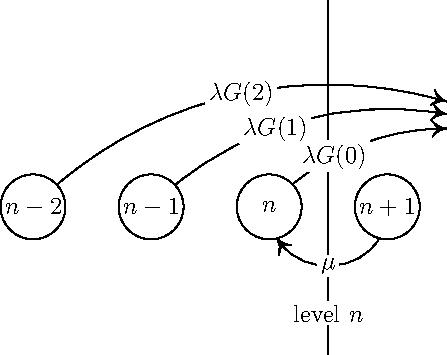
\includegraphics[scale=0.9]{mxm1_2}
%&
%    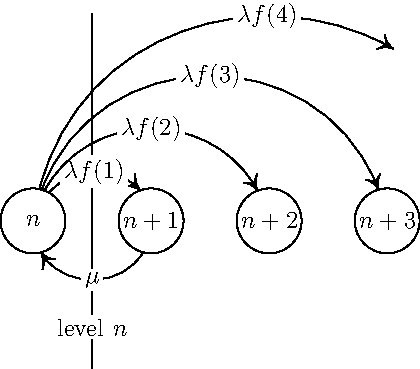
\includegraphics[scale=0.9]{mxm1_1}
%  \end{tabular}
  \caption{Level crossing of level $n$.  Observe
    that when the system is in state $n-2$, the arrival of any batch
    larger than $2$ ensures that level $n$ is crossed from below.  The
    rate at which such events happen is $\lambda G(2)$.
    Similarly, in state $n-1$ the arrival of any batch larger than one
    item ensures that level $n$ is crossed, and this occurs with rate
    $\lambda G(1)$, and so on.  
% In the right panel we see all the
%     transitions from state $n$ (the state in which the system contains
%     $n$ units of work) such that level $n$ is crossed from below.
%     Clearly, with rate $\lambda \P{X=1} = \lambda f(1)$ jobs
%     containing one item arrive; if such an event occurs, the system
%     moves from $n$ items to $n+1$ items.  With with rate
%     $\lambda f(2)$ jobs with two items work arrive, so that the system
%     contains $n+2$ units of work after the arrival of such jobs, and
%     so on. Level $n$ is crossed from above, i.e., the system moves
%     from state $n+1$ to $n$, when a unit of work is processed, which
%     happens at rate $\mu$. To relate the left and the right panel,
%     observe in the right panel that any `arrow' from state $n$ to the
%     right crosses level $n$. All these rates added together are such
%     that
%     $\lambda \sum_{i=1}^\infty f(i) = \lambda \P{B\geq 1} = \lambda
%     \P{B>0} = \lambda G(0)$.
%     A similar reasoning applied to state $n-1$ shows that only the
%     arrows such that $\lambda \sum_{i=2}^\infty f(i) = \lambda G(1)$
%     cross level $n$, and so on. 
  }
  \label{fig:levelcrossing}
\end{figure}

As always with level-crossing arguments, we turn to counting how often
level $n$ is upcrossed and downcrossed as a function of time. The
downcrossing rate is easy; it is exactly the same as for the $M/M/1$
queue. Thus, from Eq.~\eqref{eq:22}, 
\begin{equation}
\frac{D(n,t)}t = \frac{D(n,t)}{Y(n+1,t)}\frac{Y(n+1,t)}t
\end{equation}
which, as $t\to\infty$, converges to the downcrossing rate
\begin{equation}
\mu(n+1) p(n+1) = \mu \pi(n+1),
\end{equation}
where we use that $\mu(n+1) = \mu$ by the memoryless property of the
service times and PASTA to see that $\pi(n+1)=p(n+1)$.  Observe that
this part was easy because there is just one way (i.e., there is just
one arrow from right to left in Figure~\ref{fig:levelcrossing}) to
downcross level $n$, namely from $n+1$ to $n$. 

Counting upcrossings requires quite some more work. Observe that
$\1{L(A_k-)\leq n}=1$ only when the $k$th job sees~$n$ or less items in the system, and
$\1{L(A_k) > n}=1$ only when after the $k$th arrival the system contains more than $n$ items. Thus, $\1{L(A_k-) \leq n}\1{ L(A_k)>n}=1$ only when the $k$th arrival generates an upcrossing of level~$n$. 
%  Hence
% \begin{equation*}
%   \sum_{k=1}^{A(t)} \1{L(A_k-) \leq n}\,\1{L(A_k)>n}
% \end{equation*}
% counts all upcrossings  of level $n$ up to time $t$.


From Figure~\ref{fig:levelcrossing} we see that an upcrossing can be decomposed into:
\begin{equation*}
  \begin{split}
&\1{L(A_k-) \leq n}\1{L(A_k)>n}  \\
&=  \1{L(A_k-) =n}\, \1{B_k >0} + \1{L(A_k-) =n-1}\1{ B_k >1} +\cdots + \1{L(A_k-) =0}\1{B_k > n} \\
&= \sum_{m=0}^n \1{L(A_k-) =m}\1{B_k > n-m}.
  \end{split}
\end{equation*}
In other words, paths that upcross level $n$ require that any job that
sees $m$ ($m\leq n$) in the system upon arrival must bring a batch larger
than $n-m$ items.

Next, define 
\begin{equation*}
  A(m,n,t) = \sum_{k=1}^{A(t)}\1{L(A_k-) = m}\1{B_k > n-m}
\end{equation*}
as the number of jobs up to time $t$ that see $m$ in the system upon
arrival and have batch size larger than $n-m$. 

\begin{exercise}
   Show that $A(n, n,t) = A(n,t)$, where $A(n,t)$ is defined by Eq.~\ref{eq:19}.
\begin{solution}
 $A(n,n,t)$ counts all jobs up to time $t$ that see $n$ items
    and bring at least $n-n+1=1$ unit of work. As each job brings at
    least 1 item, $A(n,n,t)$ counts all jobs that see $n$ items at
    arrival.
\end{solution}
\end{exercise}

As in Section~\ref{sec:level-cross-balance}, we are primarily intested in  long-run averages. For this purpose, observe that we can write
\begin{equation}\label{eq:16}
  \frac{A(m,n,t)}t =   \frac{A(t)}t \frac{A(m,t)}{A(t)}\frac{A(m,n,t)}{A(m,t)}.
\end{equation}
By the assumptions of Section~\ref{sec:poisson-arrivals-see},  $A(t)/t\to\lambda$ and $A(m,t)/A(t)\to\pi(m)$.  Now, provided the limit exists, we define
\begin{equation}\label{eq:1332}
\lim_{t\to\infty} \frac{A(m,n,t)}{A(m,t)} = 
\lim_{t\to\infty} \frac{\sum_{k=1}^{A(t)}\1{L(A_k-) = m, B_k > n-m}}
{\sum_{k=1}^{A(t)}\1{L(A_k-) = m}}=\P{B>n-m\given L(A-)=m},
\end{equation}
where the random variable $L(A-)$   denotes the number in the system seen by an arbitrary arrival.

\begin{exercise}
Show that $\P{B>n-m\given L(A-)=m}=\P{B>n-m}$
\begin{solution}
  \begin{hint}
    Realize that $B$ and $L(A-)$ are assumed to be independent.
  \end{hint}
\begin{equation*}
  \begin{split}
\P{B>n-m\given L(A-)=m} &=
\frac{\P{B>n-m,L(A-)=m}}{\P{L(A-)=m}}\\
&=\frac{\P{B>n-m}\P{L(A-)=m}}{\P{L(A-)=m}} = \P{B>n-m}.
  \end{split}
\end{equation*}
\end{solution}
\end{exercise}

By the above exercise,
\begin{equation*}
\lim_{t\to\infty} \frac{A(m,n,t)}{A(n,t)} = \P{B>n-m} = G(n-m).
\end{equation*} 
By combining the above and making the usual assumptions about the
existence of all limits involved we find
\begin{equation*}
\lim_{t\to\infty}   \frac{A(m,n,t)}t = \lambda \pi(m) G(n-m).
\end{equation*}

\begin{exercise}
Provide an interpretation of the above result in terms of a thinned Poisson arrival process.
\begin{solution}
Eq.~(\ref{eq:16}) has the interpretation that the rate at which
level $n$ is crossed from below from state $m$ is equal the rate at
which jobs arrive times the fraction of jobs that see $m$ jobs in the
system times the fraction of jobs with batch size larger than $n-m$.
Observe that the stream of jobs with batch size larger than $n-m$
is a Poisson process thinned at rate $G(n-m)$. 
\end{solution}
\end{exercise}


The last step is to relate the up- and downcrossing rates.  Clearly, $\sum_{m=0}^n A(m,n,t)$ is  the total number of times level $n$ is upcrossed up to time~$t$. By level crossing,
 \begin{equation*}
 \sum_{m=0}^n A(m,n,t) \approx  D(n,t). 
\end{equation*}
Thus, taking the limit $t\to\infty$ in this equation, we conclude that
\begin{equation}\label{eq:42}
\lambda  \sum_{m=0}^n G(n-m) \pi(m) = \mu \pi(n+1).
\end{equation}

\begin{exercise}
  Show that Eq.~(\ref{eq:42}) reduces to $\mu p(n+1)=\lambda p(n)$ for the $M/M/1$ case.
  \begin{solution}
    The left hand side of Eq.~(\ref{eq:42}) is identical, so we only
    have to concentrate on the right hand side. In the $M/M/1$ queue,
    all batches have size $1$. Thus, $\P{B=1} = f(1)=1$ and $f(k)=0$
    for $k\neq 1$. Thus, $G(0)=1$ and $G(1)=G(2)=\cdots = 0$. Thus,
    $\sum_{m=0}^n G(n-m) p(m) = G(0)p(n)=p(n)$.
  \end{solution}
\end{exercise}

\begin{exercise}\label{ex:13}
With $\alpha = \lambda/\mu$,  show that that \emph{unnormalized} state probabilities are given by
\begin{align*}
\pi(0) & = 1 &
  \pi(1) &= \alpha \\
  \pi(2) &= \alpha^2 + \alpha G(1), &
  \pi(3) &= \alpha[ \alpha^2 + 2 \alpha G(1)) + G(2)].
\end{align*}
We leave the rest to the computer to continue with this.
\begin{hint}
For $n=1$, we have
$\mu \pi(1) = \lambda \pi(0)=\lambda$. Use that $G(0)=1$.
\end{hint}
\begin{solution}
\begin{equation*}
  \begin{split}
  \pi(1) &= \alpha \\
  \pi(2) &= \alpha G(0) \pi(1) + \alpha G(1) \pi(0) =\alpha(\alpha+ G(1)) = \alpha^2 + \alpha G(1), \\
  \pi(3) 
&= \alpha[G(0) \pi(2) + G(1) \pi(1) + G(2) \pi(0)]  = \alpha[ \alpha^2 + 2 \alpha G(1)) + G(2)],
  \end{split}
\end{equation*}
\end{solution}  
\end{exercise}

It is left to find the normalization constant.  As this recursion does
not lead to a closed form expression for $p(n)$, such as
Eq.~\eqref{eq:23}, we need to use a criterion to stop this iterative
procedure. Finding general conditions on when to stop is not directly
easy, but a pragmatic approach is to simply stop at some (large)
number $N$ such that $p(k)\ll p(0)$ for $k>N$ and is steadily decreasing. (An interesting question, why should it decrease monotonically after some, large, $N$?)
Then take $G=\sum_{i=0}^N \pi(i)$ as the normalization
constant, so that $\pi(0)=1/G$, $\pi(1)=\alpha/G$, and so on.
While this is a practical approach, getting formal bounds on a proper size of $N$ requires more work than we can do here.

Now that we have the state probabilities, we can compute the \emph{excess probability}
\begin{equation}
  \P{L> n } = \sum_{i=n+1}^\infty \pi(i).
\end{equation}
This performance measure is  of interest in inventory systems or---recall the supermarket example discussed in the Introduction---when there are costs associated with the occurence of long queues. 

An interesting extension is to consider a queueing process with batch
services, i.e., the $M/M^Y/1$ queue. Construction a recursion for the
steady-state probabilities $p(n)$ for this case is not hard, in fact,
mostly analogous to Eq.~(\ref{eq:42}).  However, solving the recursion
appears to be quite a bit harder; we will not discuss this further here

\begin{exercise}
  Why is Eq.~\eqref{eq:39}, i.e., $\pi(n)=\delta(n)$, not true for the
  $M^X/M/1$ batch queue?
\begin{solution}
 Because arrivals do not occur in single units, but in batches.
\end{solution}
\end{exercise}

Let us use  recursion Eq.~(\ref{eq:42}) for $\pi(n)$ to
 derive an expression for the expected number of units of work $\E L$
 in the system.
\begin{exercise}
 Show that
\begin{equation}\label{eq:67}
  \mu \E L =\mu \sum_{n=0}^\infty n \pi(n) = \lambda \frac{\E{B^2}}2  + \lambda \E B \E L +\lambda \frac{\E B}2,
\end{equation}
\begin{hint}
Substitute the
  recursion, and carry on with the algebra. We urge the reader to try
  it, its good (necessary) practice.  Use also the results of the
  exercises of Section~\ref{sec:mxm1-queue:-expected}.  
\end{hint}
\begin{solution}
  We use that $\mu \pi(n) =\lambda \sum_{i=0}^{n-1} \pi(i) G(n-1-i)$
  and the results of the exercises of
  Section~\ref{sec:mxm1-queue:-expected} to see that
\begin{align*}
  \mu \E L
  &=\sum_{n=0}^\infty n\, \mu \pi(n), \quad \text{now substitute for $\mu \pi(n)$ the above recursion}, \\
& =\lambda \sum_{n=0}^\infty n \sum_{i=0}^{n-1} \pi(i) G(n-1-i) 
  =\lambda \sum_{n=0}^\infty n \sum_{i=0}^\infty 1\{i<n\} \pi(i) G(n-1-i) \\
& =\lambda \sum_{i=0}^\infty \pi(i) \sum_{n=0}^\infty 1\{i<n\} n G(n-1-i) 
  =\lambda \sum_{i=0}^\infty \pi(i) \sum_{n=i+1}^\infty n G(n-1-i) \\
& =\lambda \sum_{i=0}^\infty \pi(i) \sum_{n=0}^\infty (n+i+1) G(n) 
  =\lambda \sum_{i=0}^\infty \pi(i) \left[\sum_{n=0}^\infty n G(n) +(i+1) \sum_{n=0}^\infty G(n)\right]  \\
  &=\lambda \sum_{i=0}^\infty \pi(i)\sum_{n=0}^\infty n G(n) +\lambda  \E B \sum_{i=0}^\infty \pi(i) (i+1)  \\ 
  &=\lambda \sum_{i=0}^\infty \pi(i) \frac{\E B^2 -\E B}2  + \lambda \E B (\E L +1)  \\ 
  &= \lambda \frac{\E B^2 -\E B}2  + \lambda \E B \E L +\lambda \E B \\
  &= \lambda \frac{\E B^2 }2  + \lambda \E B \E L +\lambda \frac{\E B}2,
\end{align*}
\end{solution}
\end{exercise}

With this we can check a result of Section~\ref{sec:mxm1-queue:-expected}.  
\begin{exercise}
  Use Eq.~(\ref{eq:67}) and the definition for
  $\rho=\lambda \E B/\mu$ to show that
\begin{equation*}
(1- \rho) \E L = \frac{\lambda}\mu \frac{\E{B^2}}2 + \frac\rho2.
\end{equation*}
\begin{hint}
Divide both sides by $\mu$.
\end{hint}
\begin{solution}
Dividing both sides by $\mu$ and using that $\lambda \E B/\mu = \rho$, 
\begin{equation*}
  \E L = \frac{\lambda}{\mu}  \frac{\E B^2 }2 + \rho \E L + \frac\rho2.
\end{equation*}
\end{solution}
\end{exercise}



\begin{exercise}
  Implement the recursion~(\ref{eq:42}) in a computer program for the
  case $f(1)=f(2)=f(3)=1/3$ (recall $\P{B=k} =f_k$). Take $\lambda =1$
  and $\mu = 3$.  
  \begin{hint}
This is an important problem, it helps to check (numerically)
    the algebraic results we have been deriving up to
    now. Implementing the recursion is not hard, just try and see how
    far you get.
  \end{hint}
  \begin{solution}
The recursion for $n$ becomes 
\begin{equation*}
\pi(n) = \frac \lambda \mu \sum_{i=0}^{n-1} \pi(n-1-i)G(i).
\end{equation*}
Since $G(i) =0$ for $i\geq 3$ we rewrite this to 
\begin{equation*}
  \pi(n) = \frac\lambda \mu \sum_{i=0}^{\min(\{n-1,l\}} \pi(n-1-i)G(i),
\end{equation*}
where $l=3$. 

In python this reads:

\begin{pyverbatim}
p[n] = labda / mu * sum(p[n - 1 - i] * G[i] for i in range(min(n, l)))
\end{pyverbatim}

The following code carries out the recursion for the $M/M/1$ queue and compares the result to the \emph{unnormalized} probabilities $(\lambda/\mu)^n$ (unnormalized means that I do  not multiply with $1-\rho$). Thus, we can test the code right away. 

\begin{pyconsole}
import numpy as np

l = 1 # M/M/1 has batch size 1
f = np.ones(l + 1) / l # f[0] =1, f[1] = 1 
f[0] = 0 # set f[0] = 0
F = np.cumsum(f) # distribution 
G = np.ones_like(F) - F # survivor function

labda = 1
mu = 3
num = 30
p = np.ones(num)

for n in range(1, num):
    p[n] = labda / mu * sum(p[n - 1 - i] * G[i] for i in range(min(n, l)))
    print(n, p[n], (labda / mu)**n)

\end{pyconsole}
The test is convincing.

\begin{pyconsole}
l = 3
f = np.ones(l + 1) / l
f[0] = 0
F = np.cumsum(f)
G = np.ones_like(F) - F
num = 30
p = np.ones(num)
for n in range(1, num):
    p[n] = labda / mu * sum(p[n - 1 - i] * G[i] for i in range(min(n, l)))
    print(n, p[n])

\end{pyconsole}
Stopping at 30 seems ok. The last step is normalize.
\begin{pyconsole}
p /= p.sum()  # normalize
for n in range(1, num):  # print normalized results
    print(n, p[n])

\end{pyconsole}

Now that we have the probabilities we can do all experiments we like. 
\begin{pyconsole}
EL = sum(n*p[n] for n in range(len(p)))
EL 
\end{pyconsole}

It is of interest to compare this result to the equation above
Eq.~(\ref{eq:43}).


\begin{pyconsole}
EB = sum(k*fk for k,fk in enumerate(f))
EB2 = sum(k*k*fk for k,fk in enumerate(f))
EB2
rho=labda*EB/mu
RHS = labda/mu*EB2/2 + rho/2
EL=RHS/(1-rho)
EL
\end{pyconsole}

So, after all, stopping at 30 seems not quite ok: there is a slight
difference between the two expectations. Lets run the recursion up to
100, and see what we get then.

\begin{pyconsole}
num = 100
p = np.ones(num)

for n in range(1, num):
    p[n] = labda / mu * sum(p[n - 1 - i] * G[i] for i in range(min(n, l)))

p /= p.sum()  # normalize
EL = sum(n*p[n] for n in range(len(p)))
print(EL)
\end{pyconsole}
This does the job.

As a last step, I want to check Eq.~(\ref{eq:43}). In fact, I spent at least one hour to
get Eq.~(\ref{eq:43}) correct. Now I can also numerically check it.

\begin{pyconsole}
VB = EB2 - EB*EB
C2 = VB/EB/EB
EL = (1+C2)/2*rho/(1-rho)*EB + rho/(1-rho)/2
EL
\end{pyconsole}
The results agree. 
\end{solution}
\end{exercise}


\begin{exercise}(Finite queueing systems) We consider the $M^X/M/1/K$
queue, i.e., a batch queue in which at most $K$ jobs fit into the
system. When customers can be blocked, it is necessary to specify an
acceptance, or equivalently a rejection, policy. Three common rules are
\begin{enumerate}
\item Complete rejection: if a batch does not fit entirely into the system, it will be rejected completely.
\item Partial acceptance: accept whatever fits of a batch, and reject the rest.
\item Complete acceptance: accept all batches that arrive when the
  system contains $K$ or less jobs, and reject otherwise.
\end{enumerate}
Derive a set of recursions, analogous to Eq.~(\ref{eq:42}), to compute
$\pi(n)$ for these three different acceptance rules.  
\begin{hint}
This
  exercise tests your creativity and modeling skills, it is not
  analytically difficult.  The best approach to problems like this is
  to try some simple cases first. For instance, consider the case with
  batch sizes of $1$ first, then batches of sizes $1$ or $2$, and so
  on. If system contains $K$ jobs, which batches can be accepted? If
  the system contains $K-3$, say, which batch sizes can be accepted,
  which will be refused, under which acceptance policy? 
\end{hint}
\begin{solution}
  Let's first deal with complete rejection. Suppose a batch of size
  $k$ arrives when the system contains $n$ jobs. When $k+n \leq K$,
  the batch can be accepted since the entire batch will fit into the
  queue.  When, however, $k+n> K$, the batch has to be rejected. 

  Now consider an imaginary line between states with $n$ and $n+1$
  jobs in the system. This imaginary line separates the state space
  into two disjoint part: one part with states $0, 1, \ldots, n$ and
  the other part with states $n+1, n+2, \ldots, K$. We call this
  imaginary line `level $n$'.  We call an `upcrossing' a transition
  from some state $m\leq n$ to a state $l\geq n+1$. We also say in
  that case that level $n$ is `crossed from below', i.e., from some
  state $m\leq n$ to a state $l\geq n+1$. Likewise, a `downcrossing'
  of level $n$ happens when this level is crossed from `above',
  i.e. from some state $l\geq n+1$ to some state $m\leq n$.


  If the system contains $n$ jobs,  level $n$ is
  crossed from below with rate $\lambda \pi(n) \P{B \leq K-n}$.  More generally,
  when the system is in state $m\leq n$, we need a batch of at least
  $n+1-m$ to cross the $n$. Moreover, any batch larger than $K+1-m$
  gets rejected. Thus, when the system contains $m \leq n $ jobs, the
  rate at which level $n$ is crossed from below is
  \begin{equation*}
  \lambda \pi(m) \P{n+1-m\leq B \leq K+1-m} = \lambda \pi(m)
  [G(n-m)-G(K-m)].
  \end{equation*}

  Since the server serves only single items, level $n$ can only be
  crossed from above from state $n+1$. This happens at rate $\mu p(n+1)$. 

  Finally, since on the long run the number of up- and crossings must
  be the same, the up- and downcrossing rates must match. This implies
  that the balance equations becomes
  \begin{equation*}
    \mu \pi(n+1) = \lambda \sum_{m=0}^n \pi(m)   [G(n-m)-G(K-m)],
  \end{equation*}
  for $n=0,\ldots, K-1$. 

  Before we continue with the other acceptance rules, it is important
  to check this result.  In general, off-by-one errors are easily, and
  commonly, made, so we need to test the above on simple cases. 
  \begin{itemize}
  \item  If $K\to \infty$, then $G(K-m)=\P{B>K-m}\to 0$, so we get our earlier result. 
  \item Take $n=K$. Then $G(n-m)-G(K-m)=0$ for all $m$. Then the right hand side is 0, as it should.
  \item Taken $n=0$ and $K=1$, then $\mu \pi(1)= \lambda \pi(0)$. This also makes sense. 
  \item Take $n$ much smaller than $K$. If the batch size is maximally
    $2$, then for small $n$ the entire batch must fit. Let's see if
    this holds in the above formula. If $n$ much smaller than $K$,
    then also $m$ is much smaller than $K$ (since in the right hand
    size, $m\leq n$. But then $G(K-m) \leq G(2) = 0$, as it
    should. (Observe that $G$ is a decreasing function of it argument;
    its a survival function.)
  \end{itemize}

  The complete-acceptance policy is actually quite simple. As any
  batch will be accepted when $n\leq K$, the queue length is not
  bounded.  Only when the number of jobs in the system is larger than
  $K$, we do not accept jobs. 
  \begin{equation*}
    \mu \pi(n+1) = 
    \begin{cases}
      \lambda \sum_{m=0}^n \pi(m) G(n-m), & \text{ for } n\leq K,\\
      \lambda \sum_{m=0}^K \pi(m) G(n-m), & \text{ for } n> K.
    \end{cases}
  \end{equation*}

  For the partial acceptance case, any job is accepted, but the system
  only admits whatever fits. Thus, the rate at which level $n<K$ is
  crossed is not affected by this acceptance policy, and therefore,
  \begin{equation*}
    \mu \pi(n+1) = \lambda \sum_{m=0}^n \pi(m) G(n-m), 
  \end{equation*}
  for $n=0,1,\ldots, K-1$. 
\end{solution}
\end{exercise}




\Closesolutionfile{hint}
\Closesolutionfile{ans}

\opt{solutionfiles}{
\subsection*{Hints}
\input{hint}
\subsection*{Solutions}
\input{ans}
}

\clearpage

%%% Local Variables:
%%% mode: latex
%%% TeX-master: "../book"
%%% End:

% \section
[A Relation Between the $M^X/M/1$ and $M/G/1$  Queue]
{A Relation Between the $\mathbf{M^X/M/1}$ and $\mathbf{M/G/1}$  Queue}
\label{sec:relat-batch-queu}


\subsection*{Theory and Exercises}

\Opensolutionfile{hint}
\Opensolutionfile{ans}


There is an interesting relation between the $M^X/M/1$ and the $M/G/1$
queueing systems. As an example, consider the $M^{10}/M/1$ queue in
which each job corresponds to the arrival of ten items of
work. Intuitively, it is reasonable that this queueing process is
quite similar to an $M/G/1$ queue in which each job requires
approximately 10 time units. Below we will make this relation
precise. We will also use this to find another derivation of the
Pollackzek-Khintchine equation, if we consider a certain limiting
case.


The basic observation is that by discretizing the service time $S$ of
a job in an $M/G/1$ queue we can approximate $S$ by the service time
of a batch of small units of work. To make this more specific, assume
that the distibution of the service time $S$ is given. Use a grid of
size $1/n$ and take
\begin{equation}\label{eq:69}
  \P{B^{(n)} = i} = \P{ S\in\left(\frac in, \frac{i+1}n\right]}
\end{equation}
as the distribution of the batch size $B^{(n)}$. Let the service time
of one unit of the batch be exponentially distributed with mean $1/n$.
Thus, if $n$ becomes larger, the service time $S$ is represented by
ever larger batches, but such that the service time of each unit
becomes ever smaller. These arguments can be made precise in a
probabilistic sense, but here we rely on our intuition to conclude
that, in some sense, $B^{(n)}/n \to S$\footnote{For the interested, this is convergence in distribution here.}.

\begin{exercise}
Why do we consider $\P{B^{(n)} = i} = \P{ S\in(i/n, (i+1)/n]}$ rather than
\begin{equation*}
\P{B^{(n)} = i} = \P{S\in[i/n, (i+1)/n]},  
\end{equation*}
i.e., we use a half open interval $(,]$ rather than the closed
interval $[,]$?
\begin{solution}
  Starting from the distribution function $\P{S\leq x}$, we define
  \begin{equation*}
  \P{B^{(n)} = i} = \P{ S\leq (i+1)/n} - \P{S\leq i/n} = \P{
  S\in(i/n, (i+1)/n]}.
     \end{equation*}
\end{solution}
\end{exercise}


Let us see how this limit can be used to show that the expected
waiting in queue for the batch queue leads to the
Pollackzek-Khintchine equation, i.e., the expected waiting time in
queue for the $M/G/1$ queue.  Writing $\E{L^{(n)}}$ for the batch
queue with grid size $1/n$, we use~\eqref{eq:43} to see that
\begin{align}\label{eq:1pp}
\frac{\E{L^{(n)}}}{n}
= \frac{\rho}{1-\rho}\cdot \frac12\left(1 + \frac{\V{B^{(n)}}}{(\E{B^{(n)}})^2}\right) \frac{\E{B^{(n)}}}n +  \frac1{2n}\frac{\rho}{1-\rho}.
\end{align}
By assumption\footnote{ Here we interchange limits and expectations. A
  formal approach should pay due attention to the validity of all
  these interchanges.}:
\begin{align*}
\frac{B^{(n)}}n &\to S \\
\intertext{so that must be that
}
\E{\frac{B^{(n)}}n} &\to \E S \\
\intertext{and}
\E{\frac{(B^{(n)})^2}{n^2}} &\to \E{S^2},
\end{align*}
as $n\to \infty$.  
Hence, 
\begin{equation*}
  \begin{split}
\frac{\V{B^{(n)}}}{n^2} 
&=  
\frac{\E{(B^{(n)})^2} - (\E{B^{(n)}})^2}{n^2} = 
\E{\frac{(B^{(n)})^2}{n^2}} - \left(\E{\frac{B^{(n)}}{n}}\right)^2 \\
&\to \E{S^2} - (\E{S})^2  =  \V{S}.
  \end{split}
\end{equation*}
from which
\begin{equation*}
\frac{\V{B^{(n)}}} {(\E{B^{(n)}})^2} = \frac{\V{B^{(n)}}}{n^2}\frac{n^2}{(\E{B^{(n)}})^2} \to 
\frac{\V S}{(\E S)^2} = C_s^2,
\end{equation*}
as $n\to \infty$.  Moreover, we \emph{expect} that
\begin{equation*}
\frac{\E{L^{(n)}}}n \to \E{W_Q},
\end{equation*}
since the number of items in the system, $\E{L^{(n)}}$, becomes ever
larger as $n$ increases, but the service time of one item is $1/n$,
which becomes ever smaller. Now, taking the limit $n\to\infty$
in~\eqref{eq:1pp} we obtain
\begin{equation*}
  \frac{\E{L^{(n)}}}{n}
  \to \frac{\rho}{1-\rho}  \frac{1 + C_s^2}2\E{S}.
\end{equation*}
Thus, based on this  limit we expect that 
\begin{equation*}
\E{W_Q}=  \frac{\E{L^{(n)}}}{n}
  \to \frac{\rho}{1-\rho}  \frac{1 + C_s^2}2\E{S},
\end{equation*}
but this is the same as Eq.~\eqref{eq:710}!

\begin{exercise}
  Why do we consider $\E{L^{(n)}}/n \to \E{W_Q}$, and not
  $\E{L^{(n)}}/n \to \E W$? 
  \begin{hint}
What is the expected service time of one
  unit of a job in the $M^X/M/1$ queue in the limiting case?
  \end{hint}
  \begin{solution}
    The time it takes to serve one unit is $1/n$. Thus, the fraction
    of time an item spends in service in the batch queue becomes negligible compared
    to the time in queue. Another way to see this, is to use 
    \begin{equation*}
      \frac{\E{L^{(n)}}}n = 
      \frac{\E{L^{(n)}_Q}}n + \frac{\E{L^{(n)}_s}}n.
    \end{equation*}
Since $L^{(n)}_s \leq 1$, $\E{L^{(n)}}/n \approx \E{L^{(n)}_Q}/n$ for $n$ large.
  \end{solution}
\end{exercise}

\begin{comment}
  
\begin{exercise}[use=false]
Can you model the $M^X/M/1$ as an $M/G/1$ queue, thereby deriving Eq.~(\ref{eq:43}) from Eq.~(\ref{eq:710})? 
  \begin{solution}
I guess this is a bit hard, so I include a partial answer for the interested. 


Starting from the $M/G/1$ queue, suppose first that the service time
$S$ is an exponential random variable with mean $1/\mu$.  Then the
$M/G/1$ reduces to the $M/M/1$ queue, which is evidentally equal to
the $M^1/M/1$ queue in which the jobs arrive as single units. Next, if
$S$ consists of the sum of $k$ i.i.d. exponential random variables
$S_i$ with mean $1/\mu$, i.e., $S=\sum_{i=1}^k S_i$, then the
$M^k/M/1$ queue results. Generalizing still further, we can take a
random batch $B$ of i.i.d. exponentials so that $S = \sum_{i=1}^B S_i$. Now
\begin{equation*}
  \P{S\leq x}
= \sum_{k=1}^\infty \P{S \leq x\given B=k}\P{B=k}
= \sum_{k=1}^\infty f(k) \P{\sum_{i=1}^B X_i \leq x}
\end{equation*}
where $f(k)=\P{B=k}$, and we obtain the $M^X/M/1$ from the $M/G/1$
queue by taking this distribution function for the service times.
  \end{solution}
\end{exercise}
\end{comment}

% the distribution $F$ of the service times of the $M/G/1$ on a grid of size $1/n$, like so:
% \begin{equation*}
%   F^{(n)}(x) = F(\lceil nx \rceil/n). 
% \end{equation*}
% Then $F^{(n)}(x) \downarrow F(x)$ for all $x$; recall that $F(x)$ is a
% distribution function, i.e., right continuous, non-decreasing, and such
% that $F(0) = 0$ and $F(\infty) = 1$. 







\Closesolutionfile{hint}
\Closesolutionfile{ans}

\opt{solutionfiles}{
\subsection*{Hints}
\input{hint}
\subsection*{Solutions}
\input{ans}
}
\clearpage
%%% Local Variables:
%%% mode: latex
%%% TeX-master: "../book"
%%% End:

%\input{mm1transient}
%\section
[$M/G/1$ Queue Length Distribution]
{$\mathbf{M/G/1}$ Queue Length Distribution}
\label{sec:distr-queue-length}


\subsection*{Theory and Exercises}

\Opensolutionfile{hint}
\Opensolutionfile{ans}


In Section~\ref{sec:batch-arrivals} we used level-crossing arguments 
to find a recursive method to compute  the stationary distribution $p(n)$ of the number of items in an $M^X/M/1$ queue. Here we apply similar arguments to find $p(n)=\P{L=n}$ for the $M/G/1$ queue.
However, we cannot simply copy the derivation of the $M^X/M/1$ queue to the $M/G/1$ queue, because in the $M^X/M/1$ queue the service times of the items are exponential,
hence memoryless, while in the $M/G/1$ this is not the case. When job service times are 
not memoryless, hence do not restart at arrival times, we cannot choose any moment we like to apply level-crossing. Thus, for the $M/G/1$ queue
we need to focus on moments in time in which the system `restarts', which as we will see are job departure epochs.  All in all, the argumentation to find the recursion for $\{p(n)\}$ is quite subtle, as it uses an interplay of the PASTA property and relation~\eqref{eq:39}
between $\pi(n)$, $p(n)$ and $\delta(n)$.  

An important role below is played by  the number of  arrivals $Y_k$ during the service time of the $k$th job.  Since the service times of the jobs for an i.i.d. sequence of random variables, the sequence $\{Y_k\}$ is also i.i.d. Let $Y$ be the common random variable with probability mass
 $f(j) = \P{Y = j}$; write $G(j) = \P{Y_k > j}$ for the survivor function.


\begin{exercise}
 Explain that if the service time is constant and equal to $s$, then
\begin{equation}\label{eq:4}
  \P{Y_k = j\given S=s} = e^{-\lambda s}\frac{(\lambda s)^j}{j!}.
\end{equation}
\begin{hint}
If $s$ is deterministic, the number of arrival during a fixed
    period of time with length $s$ must be Poisson distributed.
\end{hint}
  \begin{solution}
See the hint.  The period during which the arrivals occur is $s$. 
  \end{solution}
\end{exercise}

\begin{exercise}
 Explain that 
\begin{equation}\label{eq:10}
  \P{Y_k = j} = \int_0^\infty e^{-\lambda x}\frac{(\lambda x)^j}{j!}\, \d F(x).
\end{equation}
where $F$ is the distribution of the service times.
\begin{solution}
  We use a conditioning argument to arrive at this result. The
  probability that the service time is $x$ units long is written in
  various ways in the literature: $F(\d x) = \d F(x) = \P{S\in \d x}$,
  but this all means the same thing, it is only the notation that
  differs.  (As an aside, to properly define this we need measure
  theory). When $F$ has a density $f$, then
  $\d F(x) = f(x) \d x$.  Note that when $S$ is discrete, it does not
  have a density everywhere. With this,
    \begin{equation*}
    \P{Y_k=j} = \int_0^\infty \P{Y_k =j\given S=x}\P{S\in \d x} =
    \int_0^\infty \P{Y_k =j\given S=x} \d F(x).
    \end{equation*}
    Using the answer of the previous problem we arrive at the result.
\end{solution}
\end{exercise}

\begin{exercise}
  If $S$ is deterministic and equal to $s$, show that
  Eq.~\eqref{eq:10} reduces to Eq.~\eqref{eq:4}.  
  \begin{hint}
 $S=s$ then
    $\P{S=s}=1$, i.e., all probability mass lies at $s$. Thus, all
    arrivals must occur during $[0,s]$.
  \end{hint}
  \begin{solution}
    Let us first attack this problem from a general point of
    view. Suppose the service time $S$ can take values
    $s_1<s_2<\cdots <s_n$, and $\P{S=s_i}=\alpha_i$. Then of course we
    want that $\P{S\leq s_n} = \sum_{i=1}^n \alpha_i = 1$. The
    distribution function $F$ of $S$ is in this case a step function,
    with steps at the points $s_1, s_2, \ldots$, and step sizes
    $\alpha_1, \alpha_2, \ldots$. Thus, $F(s_i)-F(s_i-)=\alpha_i$. We
    say that such a distribution function has \emph{atoms} at the
    points $s_1, s_2, \ldots$. In this case we write
  \begin{equation*}
    \int_0^\infty g(x) \d F(x) = \sum_{i=1}^n g(s_i) \alpha_i.
  \end{equation*}
  Thus, the integral of $g$ with respect to $F$ is the sum of $g$ at
  the points at which $F$ makes a jump times the weight of $F$ at
  these points. 

  As an example, in case $S\equiv 10$ (the service time is always 10
  time units long) the distribution function $F$ makes just one jump
  at $s_1=10$ of size $\alpha_1 = F(10)-F(10-) =1$, i.e., $F$ has the
  form
    \begin{equation*}
      F(x) = 
      \begin{cases}
        0, &\quad x< 10, \\
        1, &\quad x\geq 10.
      \end{cases}
    \end{equation*}
With this, 
\begin{equation*}
  \int_0^\infty g(x) \d F(x) = \sum_{i=1}^n g(s_i) \alpha_i = g(s_1) \alpha_1 = g(10) \cdot 1 = g(10).
\end{equation*}
Thus, the integral of $g$ with respect to this distribution $F$ is
$g(10)$.  More generally, when $F$ puts all probability mass at the
single point $s$ (rather than at the point $10$), then
\begin{equation*}
  \int_0^\infty g(x) \d F(x) = g(s).
\end{equation*}

    Let us now copy the formula of the previous problem:
    \begin{equation*}
    \P{Y_k=j} = \int_0^\infty \P{Y_k =j\given S=x} \d F(x).
    \end{equation*}
    We see that here the integrand is the function
    $g(x) = \P{Y_k=j\given S=x}$. It is given in the question that $F$
    puts all mass on the point $s$. Therefore,
    \begin{equation*}
    \P{Y_k=j} = \int_0^\infty \P{Y_k =j\given S=x} \d F(x) = 
\int_0^\infty g(x) \d F(x) = g(s) \qquad \star
    \end{equation*}

    Now we also know that if the service time takes precisely $x$ time
    units, the number of arrivals is Poisson distributed. Therefore
    \begin{equation*}
    \P{Y_k =j\given S=x} = e^{-\lambda x}\frac{(\lambda x)^j}{j!}.
    \end{equation*}
Hence, 
    \begin{equation*}
    g(x) = \P{Y_k =j\given S=x} = e^{-\lambda x}\frac{(\lambda x)^j}{j!}.
    \end{equation*}


    Finally, using $(\star)$, and taking $x=s$ in the above expression of $g$, we get
    \begin{equation*}
    \P{Y_k=j} = \int_0^\infty \P{Y_k =j\given S=x} \d F(x) = 
    g(s) = e^{-\lambda s}\frac{(\lambda s)^j}{j!}.
    \end{equation*}
  \end{solution}
\end{exercise}

\begin{exercise}
 If $S\sim \exp(\mu)$, show that 
  \begin{equation} \label{eq:41}
f(j) = \P{Y_k = j} = \frac{\mu}{\lambda+\mu}\left(\frac{\lambda}{\lambda+\mu}\right)^j.
  \end{equation}
  \begin{solution}
Use conditional probability to see that 
\begin{equation*}
  \begin{split}
  \P{Y_n = j} 
&= \int_0^\infty e^{-\lambda x}\frac{(\lambda x)^j}{j!}\, \d F(x) = \int_0^\infty e^{-\lambda x}\frac{(\lambda x)^j}{j!} \mu e^{-\mu x}\, \d x \\
&= \frac{\mu}{j!}\lambda^j \int_0^\infty e^{-(\lambda+\mu) x}x^j\,\d x = \frac{\mu}{j!}\left(\frac{\lambda}{\lambda+\mu}\right)^j \int_0^\infty e^{-(\lambda+\mu) x}((\lambda+\mu)x)^j\,\d x \\
&= \frac{\mu}{j!}\left(\frac{\lambda}{\lambda+\mu}\right)^j \frac{j!}{\lambda+\mu}.
\end{split}
\end{equation*}
Here I also used the hints and  results of Exercise~\ref{ex:33}.

In hindsight, this result could have been derived in another way, in
fact by using the result of Exercise~\ref{ex:3} in which we analyzed a
merged Poisson process. Consider the Poisson process with rate
$\lambda+\mu$ that arises when the arrival and service process are
merged. The probability that an arrival corresponds to an epoch of the
merged process is $\lambda/(\lambda+\mu$ and the probability that a
departure corresponds to an epoch of the merged process is
$\mu/(\lambda+\mu)$.  The probability that $j$ arrivals occur before a
service occurs, is the same as the probability that a geometrically
distributed random variable with success probability
$\mu/(\lambda+\mu) = 1-p$ takes the value $j$.
  \end{solution}
\end{exercise}

\begin{exercise}
 If $S\sim \exp(\mu)$, show that 
  \begin{equation}
G(j) = \sum_{k=j+1}^\infty f(k) =  \left(\frac{\lambda}{\lambda+\mu}\right)^{j+1}.
  \end{equation}
\begin{solution}
  Take $\alpha = \lambda/(\lambda+\mu)$ so that
  $f(j) = (1-\alpha) \alpha^j$.
\begin{equation*}
  \begin{split}
  G(j) 
&= \sum_{k=j+1}^\infty f(k)  = (1-\alpha) \sum_{k=j+1}^\infty \alpha^k \\
& = (1-\alpha) \sum_{k=0}^\infty \alpha^{k+j+1}, \text{ by change of variable}\\
& = (1-\alpha) \sum_{k=0}^\infty \alpha^{k}\alpha^{j+1}= (1-\alpha)\alpha^{j+1} \sum_{k=0}^\infty \alpha^k \\
&= (1-\alpha)\alpha^{j+1} \frac{1}{1-\alpha} = \alpha^{j+1}.
  \end{split}
\end{equation*}
    \end{solution}
\end{exercise}

Let us concentrate on a downcrossing of level $n$, see
Figure~\ref{fig:mg1_2}; recall that level $n$ lies between states $n$
and $n+1$. For job $k$ to generate a downcrossing of level $n$, two events must take place: 
 job `$k-1$' must leave $n+1$ jobs behind after its service completion, and  job $k$ must leave $n$ jobs behind. Thus, 
 \begin{equation*}
   \text{Downcrossing of level $n$} \iff \1{L(D_{k-1}) = n+1}\1{L(D_k)=n} = 1.
 \end{equation*}
Let us write this in another
way. Observe that if $L(D_{k-1})=n+1$ and no other jobs arrive during
the service time $S_k$ of job $k$, i.e., when $Y_k=0$, it must also be
that job $k$ leaves $n$ jobs behind. If, however, $Y_k>0$, then
$L(D_k)\geq n+1$.  Thus, we see that
 \begin{equation*}
   \text{Downcrossing of level $n$} \iff \1{L(D_{k-1}) = n+1}\1{Y_k=0} = 1.
 \end{equation*}
% \begin{equation*}
%   \1{L(D_{k-1}) = n+1}\1{L(D_k)=n} =  \1{L(D_{k-1}) = n+1}\1{Y_k=0}.
% \end{equation*}
Consequently, the number of downcrossings of level $n$ up to time $t$ is
\begin{equation*}
  \begin{split}
  D(n+1, 0, t) 
%&= \sum_{k=1}^\infty \1{D_{k}\leq t}\1{L(D_{k})=n} \\
&= \sum_{k=1}^{D(t)}\1{L(D_{k-1})=n+1}\1{Y_k=0}.
  \end{split}
\end{equation*}

\begin{exercise}
Use a similar derivation as in~\eqref{eq:1332} to   show that 
\begin{equation*}
  \lim_{t\to\infty} \frac{  D(n+1, 0, t)}t  = \delta \delta(n+1) f(0),
\end{equation*}
where $f(0)=\P{Y=0}$.
\begin{solution}
By using the definitions and limits developed in
Sections~\ref{sec:rate-stability} and~\ref{sec:poisson-arrivals-see},
\begin{equation*}
  \begin{split}
  \lim_{t\to\infty} \frac{  D(n+1, 0, t)}t 
&=   \lim_{t\to\infty}  \frac{D(t)}t \frac{D(n+1, t)}{D(t)}\frac{ D(n+1, 0, t)}{D(n+1,t)} \\
&=   \delta \delta(n+1) \lim_{t\to\infty} \frac{ D(n+1, 0, t)}{D(n+1,t)} \\
&=   \delta \delta(n+1) \P{Y=0}\\
& = \delta \delta(n+1) f(0),
  \end{split}
\end{equation*}
where the last limit follows from the independence of $Y_k$ and
$L(D_{k-1})$, 
\end{solution}
\end{exercise}

\begin{figure}[tb]
  \centering
                  
\begin{tikzpicture}[->,>=stealth',shorten >=1pt,auto,node distance=2.8cm,
                    semithick]
\node[state] (0) {$\delta(0)$}; 
\node[state] (1) [right of=0] {$\delta(1)$}; 
\node[state] (2) [right of=1] {$\delta(2)$}; 
\node[state] (3) [right of=2] {$\delta(3)$}; 
\node[state] (4) [right of=3] {$\delta(4)$}; 
%\node[state] (5) [right of=4] {$\cdots$}; 
\node (5) [above of=4] {};

\path 
(0) edge [bend left] node[above, very near start, fill=white] {$G(3)$} (5)
(0) edge [loop below] node[below, midway, fill=white] {$f(0)$} (0)
(1) edge [bend left] node[above, very near start, fill=white] {$G(3)$} (5)
(1) edge [loop below] node[below, midway, fill=white] {$f(1)$} (1)
(1) edge [bend left] node[below, midway, fill=white] {$f(0)$} (0)
(2) edge [bend left] node[above, very near start, fill=white] {$G(2)$} (5)
(2) edge [bend left] node[below, midway, fill=white] {$f(0)$} (1)
(2) edge [loop below] node[below, midway, fill=white] {$f(1)$} (2)
(3) edge [bend left] node[above, very near start, fill=white] {$G(1)$} (5)
(3) edge [loop below] node[below, midway, fill=white] {$f(1)$} (3)
(3) edge [bend left] node[below, midway, fill=white] {$f(0)$} (2)
(4) edge [bend left] node[below, near start] {$f(0)$} (3);

% \node[circ, right=of n-2] (n-1) {$n-1$}
% edge[loop below, thick]  node[midway, fill=white] {$\lambda f(0)$} (n-1); 

\draw[-, dotted, gray] (9.7,-1)--(9.7, 4.0) node[below, black] {level $3$};


\end{tikzpicture}
\caption{Level $3$ is crossed from below with rate
  $\delta\delta(0)G(3) + \delta\delta(1)G(3) + \cdots \delta \delta(3) G(1)$ and crossed
  from above with rate $\delta\delta(4) f(0)$. }
\label{fig:mg1_2}
\end{figure}

Before we deal with the upcrossing, it is important to do the next exercise.
\begin{exercise} Suppose that $L(D_{k-1})>0$. Why is
  $S_k = D_k - D_{k-1}$?  However, if $L(D_{k-1}) = 0$, the time between
  $D_{k-1}$ and $D_k$ is \emph{not} equal to $S_k$. Why not? Can you find an expression for
  distribution of $D_k-D_{k-1}$ in case $L(D_{k-1})=0$?
  \begin{hint}
Realize that if $L(D_{k-1})=0$, job $k-1$ leaves behind an empty
  system. Thus, before job $k$ can leave, it has to arrive. In other
  words, $D_{k-1}<A_k$.  Since job $k$ arrives to an empty system,
  his service starts right away, to that the time between $A_k$ and
  $D_k$ is equal to the service time of job $k$.
  \end{hint}
\begin{solution}
  When $L(D_{k-1})>0$, job $k$ is already in the system when job $k-1$
  finishes its service and leaves. Thus, at the departure time
  $D_{k-1}$ of job $k-1$, the service of job $k$ can start right away
  at $D_{k-1}$. Then, $D_k=D_{k-1}+S_k$.


    When job $k-1$ leaves an empty system behind, $D_k= A_k + S_k$,
    since job $k$ sees an empty system, hence its service can start
    right away after its arrival time at time $A_k$. Since the arrival
    process is Poisson by assumption, the time to the next arrival
    after $D_{k-1}$ is exponentially distributed with rate
    $\lambda$. (Recall the memoryless property of the interarrival
    times.) Thus, $A_k - D_{k-1}$ has the same distribution as $X_k$,
    so that $\P{D_k - D_{k-1} \leq x} = \P{X_k + S_k\leq x}$. BTW: Can
    you simplify this expression by using conditioning on $X_k$?
\end{solution}
\end{exercise}

For the upcrossings, assume first that $L(D_{k-1})=n>0$.  Then an upcrossing of level $n>0$  must have occurred when $L(D_k)>n$, i.e, 
 \begin{equation*}
 \1{L(D_{k-1}) = n}\1{L(D_k)>n} = 1 \implies   \text{Upcrossing of level $n$}.
 \end{equation*}
Again, we can convert this into a statement about  the number of
arrivals $Y_k$ that occurred during the service time $S_k$ of job $k$.  If $Y_k=0$, then
job $k$ must leave $n-1$ jobs behind, so no upcrossing can
happen. Next, if $Y_k=1$, then job $k$ leaves $n$ jobs behind, so
still no upcrossing occurs. In fact, level $n$ can only be  upcrossed from level $n$ if
more than one job arrives during the service of job $k$, i.e.,
\begin{equation*}
\1{L(D_{k-1})=n} \1{Y_{k}>1}  \implies   \text{Upcrossing of level $n$}.
\end{equation*}
More generally, level $n$ is upcrossed from level $m$, $0<m\leq n$ whenever
\begin{equation*}
\1{L(D_{k-1})=m} \1{Y_{k}>n-m+1}  \implies   \text{Upcrossing of level $n$}.
\end{equation*}
However,  if $m=0$ (think about this),
\begin{equation*}
\1{L(D_{k})>n} = \1{L(D_{k-1})=0} \1{Y_{k}>n}   \implies   \text{Upcrossing of level $n$}.
\end{equation*}

Again we define proper counting functions,  divide by $t$, and take suitable limits to find for upcrossing rate
\begin{equation}\label{eq:555}
\delta \delta(0) G(n) + \delta \sum_{m=1}^n \delta(m) G(n-m+1).
\end{equation}

\begin{exercise}
Provide the details behind the derivation of Eq.~\ref{eq:555}.
\begin{hint}
Define for $m=1,\ldots, n$
\begin{equation*}
  D(m, n, t) = \sum_{k=1}^{D(t)}\1{L(D_{k-1})=m}\1{Y_k>n-m+1},
\end{equation*}
and 
\begin{equation*}
  D(0, n, t) = \sum_{k=1}^{D(t)}\1{L(D_{k-1})=0}\1{Y_k>n}.
\end{equation*}
Then, divide by $D(n,t)$ and $D(t)$ and take limits.
\end{hint}
\begin{solution}
With the definition of the hint, 
\begin{equation*}
  \begin{split}
  \lim_{t\to\infty} \frac{  D(0, n, t)}t 
&=   \lim_{t\to\infty}  \frac{D(t)}t \frac{D(0, t)}{D(t)}\frac{ D(0, n, t)}{D(0,t)} \\
&=   \delta \delta(0) \lim_{t\to\infty} \frac{ D(0, n, t)}{D(0,t)} \\
&=   \delta \delta(0) \P{Y>n}\\
& = \delta \delta(0) G(n).
  \end{split}
\end{equation*}

\begin{equation*}
  \begin{split}
  \lim_{t\to\infty} \frac{  D(m, n, t)}t 
&=   \lim_{t\to\infty}  \frac{D(t)}t \frac{D(m, t)}{D(t)}\frac{ D(m, n, t)}{D(m,t)} \\
&=   \delta \delta(m) \lim_{t\to\infty} \frac{ D(m, n, t)}{D(m,t)} \\
&=   \delta \delta(m) \P{Y>n-m+1}\\
& = \delta \delta(m) G(n-m+1).
  \end{split}
\end{equation*}
\end{solution}
\end{exercise}

Equating the downcrossing and upcrossing rates and dividing
by $\delta$ gives
\begin{equation*}
  f(0) \delta(n+1) = \delta(0) G(n) + \sum_{m=1}^{n} \delta(m) G(n+1-m).
\end{equation*}
Noting that $\pi(n) = \delta(n)$, which follows from~\eqref{eq:39} and
the fact that the $M/G/1$ queue length process has one-step
transitions, we arrive at
\begin{equation}\label{eq:72}
  f(0) \pi(n+1) = \pi(0) G(n) + \sum_{m=1}^{n} \pi(m) G(n+1-m).
\end{equation}

Clearly, we have  again obtained a recursion by which we can compute, iteratively, the
state probabilities, and follow the approach sketched below Exercise~\ref{ex:13}. 



\begin{exercise}
  Clearly, the $M/M/1$ queue is a special case of the $M/G/1$
  queue. Apply Eq.~\eqref{eq:72} to the $M/M/1$ queue to obtain $p(n)=(1-\rho)\rho^n$. 
  \begin{hint}
 Define shorthands
    such as $\alpha=\lambda/(\lambda+\mu)$, so that
    $1-\alpha = \mu/(\lambda+\mu)$, and
    $\alpha/(1-\alpha) = \lambda /\mu = \rho$.  Then, with Eq.~\ref{eq:41}, $f(n) = \alpha^n(1-\alpha)$ and $G(n) = \alpha^{n+1}$.  (These results do not `come for
    `free'. Of course, it's just algebra, but please try to derive this
    yourself. Its good to hone your computational skills.)
  \end{hint}
    \begin{solution}
      Take $n=0$. Then $f(0) \pi(1) = (1-\alpha)\pi(1)$, and
      $\pi(0)G(0) = \pi(0)\alpha$. Thus,
      $\pi(1) = \pi(0)\alpha/(1-\alpha) = \rho \pi(0)$. 

For $n=1$,
\begin{equation*}
  \begin{split}
  (1-\alpha)  \pi(2) 
&= \pi(0)G(1) + \pi(1)G(1) = \pi(0)G(1)(1+\rho) \\
&= \pi(0)\alpha^2(1+\rho) = \pi(0)\alpha \alpha (1+\rho) = \pi(0)\alpha \rho.
  \end{split}
\end{equation*}
Dividing by $1-\alpha$, we get
\begin{equation*}
  \pi(2) = \pi(0)\rho^2
\end{equation*}

Finally, now that we suspect that $\pi(n) = \rho^n \pi(0)$, let's fill
it in, and see whether it checks. We divide both sides by $\pi(0)$ so
that we are left with checking that
\begin{equation*}
  \begin{split}
    (1-\alpha)\rho^{n+1} 
&= \alpha^{n+1} + \sum_{m=1}^n \rho^m \alpha^{n-m+2}  \\
&= \alpha^{n+1} + \alpha^{n+2}\sum_{m=1}^n (\rho/\alpha)^m  \\
&= \alpha^{n+1} + \alpha^{n+1}\rho \sum_{m=0}^{n-1} (\rho/\alpha)^m \\
&= \alpha^{n+1} + \alpha^{n+1}\rho \sum_{m=0}^{n-1} (\rho/\alpha)^m\\
&= \alpha^{n+1} + \alpha^{n+1}\rho \frac{1-(\rho/\alpha)^n}{1-\rho/\alpha)}\\
&= \alpha^{n+1} - \alpha^{n+1}(1-(\rho/\alpha)^n), \quad\text{as } \rho/\alpha = 1+\rho,\\
&= \alpha^{n+1}(\rho/\alpha)^n = \alpha \rho^n.\\
  \end{split}
\end{equation*}
Since $\rho=\alpha/(1-\alpha)$ we see that the left and right hand sides are the same. 

Thus we get that $\pi(n) = \delta(n) = (1-\rho) \pi(0)$; a result we
obtained earlier for the $M/M/1$ queue.
\end{solution}
\end{exercise}


\begin{exercise}
  Can you design a suitable numerical method to evaluate   Eq.~\eqref{eq:10} for more 
  general distribution functions $F$? (This topic is not strictly necessary for this course, but I hope that you study it nonetheless.)
\begin{hint}
Discretize time to  a grid of points, and   approximate the integral by a summation over the grid.
\end{hint}
  \begin{solution}
  A simple numerical method is as follows. Make a grid of
  size $\d x$, for some small number $\d x$, e.g. $\d x=1/100$, and write
  $f_i = \P{S\in(i\d x, (i+1)\d x]} = F((i+1)\d x) - F(i\d x)$. Then 
  \begin{equation*}
    \begin{split}
  \P{Y_k = j} 
&= \int_0^\infty e^{-\lambda s}\frac{(\lambda x)^j}{j!} \d F(x) 
\approx \sum_{i=1}^\infty e^{-\lambda i \d x}\frac{(\lambda i\d x)^j}{j!} f_i \d x
    \end{split}
\end{equation*}

Lets try a numerical experiment. 

\begin{pyconsole}
import numpy as np

labda = 3
mu = 4
j = 5
dx = 1 / 100


def F(x):
    return 1 - np.exp(-mu * x)


def f(x):
    return F(x + dx) - F(x)


def term(i):
    res = np.exp(-labda * i * dx)
    res *= (labda * i * dx)**j / np.math.factorial(j)
    res *= f(i*dx) * dx
    return res

\end{pyconsole}

\begin{pyconsole}
print(sum(term(i) for i in range(50)))
print(sum(term(i) for i in range(500)))
print(sum(term(i) for i in range(5000)))
\end{pyconsole}

Since I don't know when to stop the integral I just try a few values;
of course stopping the integration at $x=50$ is too small, since
$50\d x=50/100=1/2$, but I include it for illustrative
purposes. Stopping at $500$ seems ok, since the results of the last
two integrals are nearly the same. This also suggestst that
$\d x=1/100$ is sufficiently small. In general, however, one must take
care and try various values for $\d x$ and the integration limits.


For more complicated situations it is best to use a
numerical library to compute the above integral. These methods have been
designed to produce good and reliable results, and, typically, it is
very hard to improve these methods. Thus, let's try a real number
cruncher.

\begin{pyconsole}
from scipy.integrate import quad

def g(x):
    return np.exp(-labda*x) * (labda*x)**j/np.math.factorial(j) * f(x)

print(quad(g, 0, np.inf))
\end{pyconsole}

This is the same as our earlier answer.
\end{solution}
\end{exercise}


\begin{comment}
\begin{exercise}[use=false]
  To analyze the distribution of $L$ of the $M/G/1$ we concentrated on
  the departure epochs. Why will this not help to find the
  distribution of $L$ for the $M/G/c$ queue?
  \begin{solution}
    \TBD.
  \end{solution}
\end{exercise}
\end{comment}


\Closesolutionfile{hint}
\Closesolutionfile{ans}

\opt{solutionfiles}{
\subsection*{Hints}
\input{hint}
\subsection*{Solutions}
\input{ans}
}

\clearpage



%%% Local Variables:
%%% mode: latex
%%% TeX-master: "../book"
%%% End:

%   \section
[$G/G/1$  and $G/G/c$ Queue: Approximations]
{$\mathbf{G/G/1}$  and $\mathbf{G/G/c}$ Queue: Approximations}
\label{sec:gg1}


\subsection*{Theory and Exercises}

\Opensolutionfile{hint}
\Opensolutionfile{ans}





In manufacturing settings it is quite often the case that the arrival
process at a station is not Poisson. For instance, if processing times
at a station are nearly constant, and the jobs of this station are
sent to a second station for further processing, the interarrival
times at the second station must be more or less equal. Hence, in this
case, the SCV of the arrivals at the second station $C_{a,2}^2$ is
most probably smaller than 1. As a consequence the
Pollackzek-Khintchine formula for the $M/G/1$-queue can no longer be
reliably used to compute the average waiting times.  As a second,
trivial case, if the interarrival times of jobs are 1 hour always and
service times 59 minutes always, there simply cannot be queue. Thus,
the $M/G/1$ waiting time formula cannot, and should not, be applied to
approximate the average waiting time of the $G/G/1$ queue. 

There is no formula as yet by which the average waiting times for the
$G/G/1$ queue can be computed; only approximations are available. One
such simple and robust approximation is based on the following
observation. Recall  the waiting time in queue for the $M/M/1$ queue:
\begin{equation*}
  \E{W_Q(M/M/1)} = \frac{\rho}{1-\rho} \E S = 
\frac{1_a + 1_b}2 \frac{\rho}{1-\rho} \E S,
\end{equation*}
where we label the number $1$ with $a$ and $b$. When generalizing this
result to the $M/G/1$ queue we get
\begin{equation*}
  \E{W_Q(M/G/1)} = \frac{1_a + C_s^2}2 \frac{\rho}{1-\rho} \E S,
\end{equation*}
Thus, $1_b$ in the expression for the $M/M/1$ queue is replaced by
$C_s^2$ in the expression for the $M/G/1$ queue. As a second
generalization, Kingman proposed to replace $1_a$ in this formula by
the SCV of the interarrival times
\begin{equation*}
C_a^2 = \frac{\V X}{(\E X)^2}
\end{equation*}
resulting in
\begin{equation*}
  \E{W_Q(G/G/1)} \approx \frac{C_a^2 + C_s^2}2 \frac{\rho}{1-\rho} \E S.
\end{equation*}

This formula is reasonably accurate; for related expressions we refer
to \citet{bolch06:_queuein_networ_markov_chain} and
\citet{hall91:_queuein_method_servic_manuf}. With Little's law we can
compute $\E{L_Q}$ from the above. Moreover, $\E W = \E{W_Q} + \E S$,
and so on, c.f., Section~\ref{sec:some-usef-ident}



It is crucial to memorize the \emph{scaling} relations that can be
seen from the $G/G/1$ waiting time formula. Roughly:
\begin{enumerate}
\item $\E{W_Q} \sim (1-\rho)^{-1}$. The consequence is that the waiting
  time increases \emph{very steeply} when~$\rho$ is large, hence is
  very sensitive to the actual value of $\rho$ when $\rho$ is large.
\item $\E{W_Q} \sim C_a^2$ and $\E{W_Q} \sim C_s^2$. Hence, reductions
  of the variation of the interarrival and service times do affect the
  waiting time, but only linearly.
\item $\E{W_Q} \sim \E S$. Thus, working in smaller job sizes reduces
  the waiting time also. The average queue length does not decrease by
  working with smaller batches, but jobs are more `uniformly spread'
  over the queue. This effect lies behind the idea of
  `lot-splitting', i.e., rather than process large jobs, split jobs
  into multiple small jobs (assuming that setup times are negligible),
  so that the waiting time per job can be reduced.
\end{enumerate}

These insights prove very useful when trying to reduce waiting times
in any practical situation. First try to reduce the load (by blocking
demand or increasing the capacity), then try to reduce the variability
(e.g., by planning the arrival times of jobs), and finally, attempt to
split jobs into multiple smaller jobs and use the resulting freedom to
reschedule jobs in the queue.

For the $G/G/c$ queue we also only have an approximation: 
\begin{equation}\label{eq:7}
  \E{W_Q} = \frac{C_a^2+C_e^2}2 \frac{\rho^{\sqrt{2(c+1)}-1}}{c(1-\rho)} \E S.
\end{equation}


Even though the above results are only approximate, they prove to be
exceedingly useful when designing queueing systems and analyzing the
effect of certain changes, in particular  changes in capacity,
variability and service times.

\begin{exercise}($G/G/1$)
  Show that the approximation~\eqref{eq:7} reduces to the result known for the $M/M/1$ and $M/G/1$ queues.
  \begin{hint}
 Take $c=1$.
  \end{hint}
  \begin{solution}
    If $c=1$, as is the case for the $M/M/1$ queue, $\sqrt{2(c+1)} - 1=2-1=1$, so that~\eqref{eq:7} reduces to $\E{W_Q} = \rho/(1-\rho) \E S$. Recall that $C_a^2=C_s^2=1$ for the $M/M/1$. 
  \end{solution}
\end{exercise}





\begin{exercise}
  Is Eq.~\eqref{eq:24} also valid for the $G/G/1$ queue? Why (not)?
  \begin{solution}
    Not necessarily. Since jobs do not arrive in general as a Poisson
    process, we cannot use the PASTA property to conclude that the
    time average queue length $\E{L_Q}$ is the same as the average
    queue length as observed by customers.

(Can you provide an example that shows this difference?
    Hint, we did this earlier.)
  \end{solution}
\end{exercise}



\begin{exercise}
  Consider a queue $n$ servers, with generally distributed
  interarrival times, generally distributed service times, and the
  system can contain at most $K$ customers, i.e, the $G/G/n/K$ queue.
  Let $\lambda$ be the arrival rate, $\mu$ the service rate, $\beta$
  the long-run fraction of customers lost, and $\rho$  the average
  number of busy/occupied servers
  Show that 
  \begin{equation*}
    \beta = 1 - \rho\frac{\mu}{\lambda}.
  \end{equation*}
\begin{solution}
  This follows from the observation that $\lambda(1-\beta)$ is the net
  arrival rate, as jobs are lost at a rate $\lambda\beta$ . Hence, the
  load must be $\lambda(1-\beta)/\mu$. As the load must be equal to
  $\rho$, it follows that $\rho = \lambda(1-\beta)/\mu$, from which the
  other result immediately follows.
\end{solution}
\end{exercise}

\begin{exercise}
 Consider a single-server queue at which every minute a
    customer arrives, precisely at the first second. Each customer
    requires precisely $50$ seconds of service. 
What are $\rho$,
    $\E L$, $C_a^2$, and $C_S^2$?
  \begin{solution}
 $\rho = \lambda \E S = 1/60 \cdot 50 = 5/6$. Since job
      arrivals do not overlap any job service, the number of jobs in
      the system is 1 for $50$ seconds, then the server is idle for 10
      seconds, and so on. Thus $\E L = 1\cdot5/6 = 5/6$. There is no
      variance in the interarrival times, and also not in the service
      times, thus $C_a^2 = C_s^2 = 0$. Also $\E{W_Q}=0$ since
      $\E{L_Q}=0$. Interestingly, we get the same from Kingman's formula.
  \end{solution}
\end{exercise}

\begin{exercise}
 Consider the same single-server system as in the previous exercise, but now the customer
    service time is stochastic: with probability $1/2$ a customer
    requires $1$ minute and $20$ seconds of service, and with
    probability $1/2$ the customer requires only $20$ seconds of
    service.  What are $\rho$, $C_a^2$, and $C_S^2$?
  \begin{solution}
 Again $\E S$ is 50 seconds, so that $\rho = 5/6$. Also
      $C_a^2=0$. For the $C_S^2$ we have to do some work. 
      \begin{equation*}
        \begin{split}
          \E S &=  \frac{20}2 + \frac{80}2 = 50 \\
          \E{S^2} &=  \frac{400}2 + \frac{6400} 2 = 3400 \\
          \V S &=  \E S^2 - (\E S)^2 = 3400 - 2500 = 900 \\
          C_S^2 &=  \frac{\V S}{(\E S)^2} = \frac{900}{2500}=\frac{9}{25}.
        \end{split}
      \end{equation*}
  \end{solution}
\end{exercise}

It is crucial to remember from the above exercises that knowledge of the   utilization is not sufficient to characterize the average queue   length.

\begin{exercise}
  For the $G/G/1$ queue, prove that the fraction of jobs that see $n$
  jobs in the system is the same as the the fraction of departures that
  leave $n$ jobs behind. What condition have you used to prove this?
%\item Motivate that for  the $G/M/1$, $\delta(n) = p(n)$, i.e.,  departures see time averages. 
  \begin{solution}
    All follows straightaway from the definitions in the main text. In
    the $G/G/1$ queue jobs arrive and depart in single units. Hence,
    $|A(n,t)-D(n,t)|\leq 1$, c.f., Eq.~(\ref{eq:19}). Then, 
    \begin{equation*}
      \frac{A(t)}{t}\frac{A(n,t)}{A(t)} \approx 
      \frac{D(t)}{t}\frac{D(n,t)}{D(t)}. 
    \end{equation*}
    The left hand side goes to $\lambda \pi(n)$ as $t\to\infty$, and
    the right hand side to $\gamma \delta(n)$. Use the fact that we
    always assume, implicitly, that the system is stable, so that
    $\lambda = \gamma$. As a consequence $\delta(n) = \pi(n)$.
  \end{solution}
\end{exercise}

\begin{exercise}
  Suppose for the $G/G/1$ that a job sees $n$ jobs in the system upon
  arrival. Can you use the central limit law to estimate the
  distribution of waiting time in queue for this job?  
  \begin{hint}
 Let $S_n = \sum_{k=1}^n X_k$ and $\sigma_n^2 = n\V X$. Then,
    under conditions you can find on the internet,
    \begin{equation*}
    \frac{S_n - n \E X}{\sigma_n} \to \mathcal{N}(0,1), \quad\text{as } n\to \infty,
    \end{equation*}
    where $\mathcal{N}(0,1)$ is a normally distributed random variable
    with $\mu=0$ and $\sigma^2=1$. But then 
    \begin{align*}
    \frac{S_n - n \E X}{\sigma_n} &\approx  \mathcal{N}(0,1)  \iff\\
    S_n - n \E X &\approx  \sigma_n \mathcal{N}(0,1)  \iff\\
    S_n - n \E X &\approx  \mathcal{N}(0,\sigma_n^2)  \iff\\
    S_n  &\approx   n \E X + \mathcal{N}(0,\sigma_n^2)  \iff\\
    S_n  &\approx    \mathcal{N}(n \E X,\sigma_n^2),
    \end{align*}
    hence, $S_n$ is approximately distributed as
    $\mathcal{N}(n\E X, \sigma_n^2)$.
  \end{hint}
\begin{solution} If the number in the system is $n$, then the total
  service time required to process these $n$ jobs is the sum of the
  service times, i.e.,$W_{Q,k} = \sum_{k=1}^n S_k$ where $k$ counts over the
  $n$ jobs in the system. Then, with the hint,
  \begin{equation*}
    W_{Q, k} \sim  \mathcal{N}(n\E S, \sigma_n^2)
  \end{equation*}
where $\sigma_n^2 = n \V S$. 
Thus, the waiting time in queue is approximately normally distributed with mean $n \E S$ and variance $n \V S$. 
\end{solution}
\end{exercise}

\begin{exercise}
  (Hall 5.19) When a bus reaches the end of its line, it undergoes a
  series of inspections. The entire inspection takes 5 minutes on
  average, with a standard deviation of 2 minutes. Buses arrive with
  interarrival times uniformly distributed on $[3,9]$ minutes.

As a first case,  assuming a single server, estimate $\E{W_Q}$ with the $G/G/1$ waiting time formula. As a second case, compare this result to an $M/G/1$ system with arrival rate 10 per hour and the same service time distribution. Explain why your previous answer is smaller. 
  \begin{hint}
 It took me some time to understand the details of part a. I
    then decided to read part b first, which clarified the intent of
    part a.
  \end{hint}
  \begin{solution}
\begin{enumerate}
\item 
<<term=True>>=
a = 3.
b = 9. 
EA = (b+a)/2.
EA
labda = 1./EA # per minute
labda
VA = (b-a)*(b-a)/12.
CA2 = VA/(EA*EA)
CA2

ES = 5.
sigma = 2
VS = sigma*sigma
CS2 = VS/(ES*ES)
CS2

rho = labda*ES
rho

Wq = (CA2+CS2)/2. * rho/(1.-rho) * ES
Wq
@

\item 
<<term=True>>=
Wq = (1.+CS2)/2.*rho/(1.-rho)*ES
Wq
@

The arrival process with uniform interarrival times is much more
regular than a Poisson process. In the first case, bus arrivals are
spaced in time at least with 3 minutes.
  \end{enumerate}
    \end{solution}
\end{exercise}



Clearly, Kingman's equation requires an estimate of the SCV $C_a^2$ of
the interarrival times and the SCV $C_s^2$ of the service times. Now
it is not always easy in practice to determine the actual service time
distribution, one reason being that service times are often only
estimated by a planner, but not actually measured. Similarly, the
actual arrival moments of jobs are often not registered, mostly just
the date or the hour, perhaps, that a customer arrived.  Hence, it is
often not possible to estimate $C_a^2$ and $C_s^2$ from information
that is available.  However, when for instance the number of arrivals
per day have been logged for some time so that we know
$\{a_n, n=1,\ldots, N\}$ for some $N$, we can use this information
instead of the the interarrival times $\{X_k\}$ to obtain insight into
$C_a^2$.  The relation we present here to compute $C_a^2$ from
$\{a_n\}$ can of course also be applied to estimate $C_s^2$.

\begin{theorem} The SCV of the interarrival times can be estimated
  with the following formula
\begin{equation*}
C_a^2 \approx \frac{\tilde \sigma^2}{\tilde \lambda},
\end{equation*}
where 
\begin{equation*}
\tilde  \lambda = \lim_{n\to\infty} \frac 1n  \sum_{i=1}^n a_i,\quad  
\tilde  \sigma^2 = \lim_{n\to\infty} \frac 1 n \sum_{i=1}^n a_i^2 - \tilde \lambda^2,
\end{equation*}
in words, $\tilde \lambda$ is the average number of arrivals per
period, e.g., per day, and $\tilde \sigma^2 $ is the variance of the
number of arrivals per period.
\end{theorem}

\begin{proof}
  The proof is based on an argument in \cite{cox62:_renew_theor}. We
  use quite a bit of the notation developed in
  Section~\ref{sec:rate-stability}. Let $\{A(t), t\geq 0\}$ be the
  number of arrivals that occur up to (and including) time $t$. We
  assume that $\{A(t)\}$ is a renewal process such that the
  interarrival times $\{X_k, k=1, 2, \ldots\}$ with
  $X_k = A_{k}-A_{k-1}$, are i.i.d. with mean $1/\lambda$ and standard
  deviation~$\sigma$. (Observe that $\sigma$ is not the same as
  $\tilde \sigma$ above.) Note that $C_a^2$ is defined in terms of
  $\lambda$ and $\sigma$ as:
\begin{equation*}
C_a^2 = \frac{\V{X_i}}{(\E{X_i})^2} = \frac{\sigma^2}{1/\lambda^2} = \lambda^2 \sigma^2.
\end{equation*}

Next, let $A_k$ be the arrival time of the $k$th arrival. The
following useful relation between $A(t)$ and $A_k$ enables us to prove
our result (recall that we uses a similar relation in the derivation
of the Poisson process):
\begin{equation*}
\P{A(t) < k} = \P{A_k > t}
\end{equation*}

Since the interarrival times have finite mean and second moment by
assumption, we can apply the central limit law to obtain that, as
$k\to\infty$,
\begin{equation*}
\frac{A_k -k/\lambda}{\sigma \sqrt k} \to N(0,1),
\end{equation*}
where $N(0,1)$ is a standard normal random variable with
distribution $\Phi(\cdot)$.  Similarly,
%
\begin{equation*}
\frac{A(t) -\lambda t}{\alpha \sqrt t} \to N(0,1)
\end{equation*}
for an $\alpha$ that is yet to be determined. Thus,
$\E{A(t)} = \lambda t$ and $\V{A(t)}=\alpha^2 t$.

Using that $\P{N(0,1) \leq y} =
\P{N(0,1) > -y}$ (and $\P{N(0,1)=y} = 0$) we have that
%
\begin{align*}
\Phi(y) &\approx \P{\frac{A_k - k/\lambda}{\sigma \sqrt k }\leq y} \\
        &= \P{\frac{A_k - k/\lambda}{\sigma \sqrt k} >  -y} \\
        &=  \P{A_k >  \frac k\lambda - y \sigma \sqrt k}.
\end{align*}
Define for ease
\begin{equation*}
t_k = \frac{k}\lambda - y \sigma \sqrt k.
\end{equation*}
We can use the above relation between the distributions of~$A(t)$
and~$A_k$ to see that~$\P{A_k >t_k } = \P{A(t_k) <k}$. With this we
get,
\begin{align*}
\Phi(y)
        &\approx  \P{A_k >  t_k } \\
        &=  \P{A(t_k) <  k } \\
        &=  \P{\frac{A(t_k) - \lambda t_k}{\alpha \sqrt{t_k}} < 
\frac{k-\lambda t_k}{\alpha \sqrt{t_k}}}.
\end{align*}
Since, $(A(t_k) - \lambda t_k)/ \alpha \sqrt{t_k} \to N(0,1)$
as $t_k \to \infty$, the above implies that
\begin{equation*}
\frac{k-\lambda t_k}{\alpha \sqrt{t_k}} \to y,
\end{equation*}
as $t_k \to \infty$.  Using the above definition of $t_k$, the left
hand of this equation can be written as
\begin{equation*}
\frac{k-\lambda t_k}{\alpha \sqrt{t_k}} =
\frac{\lambda \sigma \sqrt k }{\alpha \sqrt{k/\lambda + \sigma\sqrt k}} y.
\end{equation*}
Since $t_k \to \infty$ is implied by (and implies)
$k\to\infty$, we therefore want that $\alpha$ is such that
\begin{equation*}
\frac{\lambda \sigma \sqrt k }{\alpha \sqrt{k/\lambda + \sigma\sqrt k}} y \to y,
\end{equation*}
as $k\to\infty$. This is precisely the case when
\begin{equation*}
\alpha = \lambda^{3/2}\sigma.
\end{equation*}
Finally, for $t$ large (or, by the same token $k$ large),
\begin{equation*}
\frac{\sigma_k^2}{\lambda_k} = \frac{\V{A(t)}}{\E{A(t)}} \approx \frac{\alpha^2 t}{\lambda t} 
= \frac{\alpha^2}{\lambda} = \frac{\lambda^3\sigma^2}{\lambda} = \lambda^2 \sigma^2 = C_a^2,
\end{equation*}
where the last equation follows from the above definition of $C_a^2$.  The proof is complete.
\end{proof}




\Closesolutionfile{hint}
\Closesolutionfile{ans}
\subsection*{Hints}
\input{hint}
\subsection*{Solutions}
\input{ans}
\clearpage

%%% Local Variables:
%%% mode: latex
%%% TeX-master: "book"
%%% End:

% \section{Service Interruptions}
\label{sec:serv-interr}

No notes; only questions.

\begin{question}
  Determine the expectation and variance of $S_N = \sum_{i=1}^N X_i$
  where $N$ is a random variable (with finite second moment) and
  $\{X_i\}$ are i.i.d. as the generic random variable $X$.
\begin{solution}
We first consider the
expectation.  If it is given that $N=n$, then
\begin{equation*}
  \E{S_N \given N=n} =  \E{\sum_{i=1}^n X_i}= \E{X_1} + \E{X_2} + \cdots \E{X_n} = n \E X,
\end{equation*}
where the last equation follows from the fact that the $X_i$ have the same distribution. With this, 
\begin{equation*}
  \E{\sum_{i=1}^N X_i} =   \E{\E{\sum_{i=1}^N X_i \given N}} =  \E{N\E{X}} = \E X \E N.
\end{equation*}
This result in known as Wald's equation. 

To compute the variance we use that $\V{S_N} =\E{S_N^2} - (\E{S_N})^2$. Thus, we first compute
\begin{equation*}
  \begin{split}
  \E{ S_N^2 \given  N=n} 
&=  \E{\left(\sum_{i=1}^n X_i\right)^2}  
=  \E{\sum_{i=1}^n X_i^2 + \sum_{i\neq j}^n X_i X_j}  \\
&= \sum_{i=1}^n \E{X^2_i} + \sum_{i \neq j} \E{X_i} \E{X_j},
  \end{split}
\end{equation*}
since $\E{X_iX_j} = \E{X_i} \E{X_j}$ by independence. Therefore, using
that the $\{X_i\}$ are i.i.d. as $X$,
\begin{equation*}
  \E{ S_N^2 \given N=n} = n \E{X^2} + n(n-1) (\E X)^2. 
\end{equation*}
With this, 
\begin{equation*}
  \begin{split}
  \E{ S_N^2}  &= \E{\E{ S_N^2 \given N=n}}  \\
&= \E{N \E X^2 + N(N-1)(\E X)^2 } \\
& = \E N \E{ X^2} + \E{N^2} (\E X)^2 - \E N (\E X)^2 \\
& = \E N (\E{ X^2}  - (\E X)^2) + \E{N^2} (\E X)^2 \\
& = \E N \V X + \E{N^2} (\E X)^2.
  \end{split}
\end{equation*}
And finally,
\begin{equation}
  \begin{split}
  \V{S_N} 
&= \E{S_N^2}  - (\E{S_N})^2 \\
&= \E N \V X + \E{N^2} (\E X)^2   - (\E N)^2 (\E X)^2 \\
&= \E N \V X + \V N (\E X)^2.
  \end{split}
\end{equation}

\end{solution}
\end{question}


\begin{question} 

  A small company receives orders at a rate $\lambda$.  After a batch
  of $B$ orders have been assembled, the company produces the batch.
  The average service time of an order is $1/\mu$. Between two batches
  the company has to re-adjust some of the machines before it can
  process another batch. A setup costs  $S$ time units.

\begin{enumerate}
\item Should the batch size be limited from above or below to ensure that the system remains stable? 
\item How many orders arrive on average during a setup?
\item Use the above two points to determine a criterion on the batch size $B$. 
\end{enumerate}

\begin{solution}
\begin{enumerate}
\item Only from below. If batches are very large, the fraction of time spent on setups becomes very small.
\item \begin{equation*}
    \lambda \E S
  \end{equation*}
Ensure you realized that you used Wald's rule.
\item  The number of jobs that arrive, on average, during one
  production cycle must be smaller than the total amount of jobs that
  can be served, on average, during one cycle.   The number of arrivals during the setup is $\lambda \E S$. The number of arrivals during serving the batch is $\lambda B/\mu$. Thus, 
  \begin{equation*}
    \lambda ( B/\mu + S) < B.
  \end{equation*}
\end{enumerate}
\end{solution}
\end{question}

\begin{question}
Zijm.Ex.1.11.1
 \begin{solution}
Yes. The availability is $93\%$. Since $\E{S_e} = \E S/A$, and if $\E S $ is known, $\E{S_e}$ follows.
\end{solution}
\end{question}

\begin{question}
Zijm.Ex.1.11.2
 \begin{solution}
   No, from Zijm.Eq.1.51, the average repair time has to be known. The
   repair time here is of course the time it takes for a mechanic to
   show up at work again.
\end{solution}
\end{question}
\begin{question}
Zijm.Ex.1.11.3
 \begin{solution}
   It might, but perhaps a normal distribution would be better. It
   makes sense to make a histogram of the recover times to see whether
   some clear pattern is present. 

   Besides this, I don't know how sensitive the result for $C_e^2$ is
   on the distribution of the repair times. Perhaps it is not that
   sensitive, so in that case it would be ok to simply use the
   exponential distribution. 

The sensitivity study would be an interesting topic for simulation. 
\end{solution}
\end{question}
\begin{question}
Zijm.Ex.1.11.4 and 1.11.5
 \begin{solution}
   We need to make an assumption about the distribution of the repair
   times. Inferring from the text, the repair time is always $2$
   days. Lets also assume that all jobs accumulate in front of the
   broken machine, in other words, the broken machine is part of the
   job routing of each job. Then
   \begin{equation*}
     \P{N(2) > 20} = 
\sum_{n=21}^\infty e^{-5\cdot 2} \frac{10^n}{n!}.
1  - \sum_{n=0}^{20} e^{-5\cdot 2} \frac{10^n}{n!} = 1-0.9984,
   \end{equation*}
i.e., very small.  This is the code I used: 

<<term=True>>=
from math import exp, factorial
exp(-10) * sum((10)**n / factorial(n) for n in range(21))
@
\end{solution}
\end{question}

\begin{question}
Zijm.Ex.1.11.4

 \begin{solution}
If the shop already contains 10 jobs, somewhere upstream of the broken machine, then 
   \begin{equation*}
     \P{N(2) > 10} = 1- 0.58.
   \end{equation*}
where  I used
<<term=True>>=
exp(-10) * sum((10)**n / factorial(n) for n in range(11))
@
\end{solution}
\end{question}

\begin{question}
Zijm.Ex.1.11.6
 \begin{solution}
   Cleaning times will be pretty constant. Changing dies, or other
   machine parts, is also typically quite predictable, although it can
   take a lot of time, in particular in case a crane or other heavy
   machinery is needed to replace parts. If the machine require
   temporary adjustments, then the variation in setup times may be
   quite a bit higher.
\end{solution}
\end{question}

\begin{question}
Zijm.Ex.1.11.7
 \begin{solution}
   Then the effective service times, and in particular, $C_e^2$ will
   be quite a bit bigger. It is preferable to avoid such a situation. 

   Mathematically, it is only given that $N_s$ is a random
   variable. As, however, this does not state anything about its
   distribution, we cannot make any general claim. The intent of the
   problem is to have you check the relevant formulas and notice that
   the variance of $N_s$ appears in the formulas.
\end{solution}
\end{question}

\begin{question}[use=false]
  Suppose a single machine workstation has to process $n$ different
  product families. Jobs of family $i$ arrive as a Poisson process
  with rate $\lambda_i$.  Service times are exponentially distributed
  with average $\mu_i^{-1}$ for family $i$. A setup of time $S$ is
  required if the machine switches from one family to another. If the
  machine works according to a cyclic schedule, i.e., produce family
  1, then 2, then 3, and so on until family $n$, Can you find batch
  sizes $B_i$ for family $i$ such that an average waiting time can be
  guaranteed?
  \begin{solution}
    \TBD. 

    This problem can be generalized and has been widely studied as one
    of the core problems in stochastic machine scheduling. For
    instance, what to do if the setup times are family-dependent, or
    even more general, dependent on the sequence in which the families
    are planned? This is a very hard problem. 
  \end{solution}
\end{question}

%%% Local Variables:
%%% mode: latex
%%% TeX-master: "notes_all"
%%% End:

%  \section{Process Batching}
\label{sec:process-batching}


\subsection*{Theory and Exercises}

\Opensolutionfile{hint}
\Opensolutionfile{ans}


\begin{exercise}
Zijm.Ex.1.12.1
 \begin{solution}
Zijm, Eq. 1.66

<<term=True>>=
labda = 10
mu = 30
ESs = 2 #days

labda*ESs/(1-labda/mu)
@

At least 30 jobs need to be served in a batch.
\end{solution}
\end{exercise}

\begin{exercise}
Zijm.Ex.1.12.2
 \begin{solution}

<<term=True>>=
N = 50
VarSs = 0 # fixed setup time
ES0 = 1/mu
VarS0 = 1/mu**2 # M/M/1, hence exponential service times

ESb = ESs + N*ES0 # Eq.1.64 Zijm

Csb2 = (VarSs + N*VarS0)/ESb**2 
Csb2

labdaB = labda/N
labdaB


rho = labdaB*ESb # Eq.1.65
rho 
@

When inspecting the SCV, I find it a bit small. To see whether I made a mistake, I'll try to make Figure 1.6 of Zijm.

<<>>=
VarSs = 0
ES0 = 1 / mu
VarS0 = 1 / mu**2  # M/M/1, hence exponential service times

for N in range(31, 120, 5):
    ESb = ESs + N * ES0  # Eq.1.64 Zijm
    Csb2 = (VarSs + N * VarS0) / ESb**2
    labdaB = labda / N
    rho = labdaB * ESb  # Eq.1.65
    Cab2 = 1 / N  # recall that Ca2=1 for M/M/1
    W = (Cab2 + Csb2) / 2 * rho / (1 - rho) * ESb + ESb
    print("{} {:f} {:f} {:f} {:f}".format(N, ESb, Csb2, rho, W))
@

This is not the same as the results of Figure 1.6. After closely
inspecting my results above, I can't find a mistake\ldots Perhaps you see what's wrong.
\end{solution}
\end{exercise}

\begin{exercise}
Zijm.Ex.1.12.3
 \begin{solution}
   Definitely bigger. Observe that the waiting time is very sensitive
   to the batch size, hence to the estimates of all involved
   parameters such as the arrival rate, service times, setup time, and
   so on. Since, in general, it is very hard to obtain good estimates
   of these data (the order portfolio changes continuously, personnel
   does not always produce the same quality, rework may result, and so
   on and so forth), one must stay away from such situations. It is
   much better to be on the safe side of things.
\end{solution}
\end{exercise}





\Closesolutionfile{hint}
\Closesolutionfile{ans}
\subsection*{Hints}
\input{hint}
\subsection*{Solutions}
\input{ans}




%%% Local Variables:
%%% mode: latex
%%% TeX-master: "notes"
%%% End:

% \section
[$M/G/1$ Queue: The density of the waiting time]
{$\mathbf{M/G/1}$ Queue: The density of the waiting time}

Level-crossing analysis is a powerful method to tackle probability
problems. Here we show how to use this method to derive an integral
equation that should be satisfied by the steady state density $f_Q$ of
the waiting time of the M/G/1 queue. This section is included for
curious readers; it can be safely skipped without interrupting the
main flow of the course. Most of the derivation below is based on
hand-waiving arguments, but all can be made mathematically rigorous,
see, e.g., \cite{brill08:_level_cross_method_stoch_model}.

The result we want to derive is the functional equation of which the
density $f_Q$ is the solution:
\begin{equation}\label{eq:51}
\begin{split}
   f_Q(x) &= \lambda \int_0^x f_Q(y) G(x-y) \,\d y + \lambda p(0) G(x), \\
   f_Q(0) &= \lambda p(0),
\end{split}
\end{equation}
where $G(x) = 1 - F(x)$ is the survivor function of the service time
$S$, and $p(0)$ is the long-run fraction of time the system is empty. 
Once we have established the above, we show how this equation can be
used to obtain the Pollaczek-Khintchine equation. In the last section
we use it to find an explicit expression for the density of the
waiting time of the M/M/1 queue.

Thus, the first step is to show how to obtain~\eqref{eq:51} by means
of level-crossing.  Write $F_Q(x,t) = \P{W_Q(t) \leq x}$ for the
probability that at time $t$ the waiting time $W_Q(t)$ is smaller or
equal to $x$. Let
%
\begin{equation*}
G_Q(x,t) = 1 - F_Q(x,t) = \P{W_Q(t) > x}.
\end{equation*}
Take $h\ll 1$. Some thought will reveal that the following must hold
%
\begin{align*}
 G_Q(x, t+h)
 &= \P{W_Q(t+h) > x} \quad\text{by definition}\\
&= \P{W_Q(t) > x+h} \quad\text{the waiting time decreases } h\text{ units in } h\text{ time units}\\
&+ \lambda h\int_0^x \P{S>x-y} \P{W_Q(t) \in \d y}\quad \text{for any customer that sees a positive waiting time} \\
&+ \lambda h \P{W_Q(t) = 0} \P{S> x}\quad \text{for any customer that arrives at an empty system}\\
&+o(h).
\end{align*}
Here $\P{W_Q(t) \in \d y}$ is a notation used to indicate that
the integration should be taken with respect to the measure induced by
the distribution $\P{W_Q(t)\leq y}$. Assuming that
$F_Q(x,t)$ has a density $f_Q(x,t)$ for all
$y>0, t\geq 0$, we can write $\P{W_Q(t) \in \d y} =
f_Q(y,t)\d y$. Using this, we see that
%
\begin{equation*}
G_Q(x, t+h)
= G_Q(x+h, t) + \lambda h \int_0^x G(x-y) f_Q(y,t) \,\d y  + \lambda h F_Q(0,t) G(x) + o(h).
\end{equation*}
Subtracting $G_Q(x+h,t)$ from both sides gives
%
\begin{equation*}
G_Q(x, t+h) -  G_Q(x+h, t) =  \lambda h \int_0^x G(x-y) f_Q(y,t) \,\d y  + \lambda h F_Q(0,t) G(x) + o(h).
\end{equation*}
Assuming that all required derivatives exist, and writing $\partial_t = \partial/\partial t$ and
$\partial_x = \partial/\partial x$, we can expand the left hand as
%
\begin{align*}
G_Q(x, t+h) -  G_Q(x+h, t)
&= G_Q(x, t+h) - G_Q(x,t) + G_Q(x,t) - G_Q(x+h, t) \\
&= h \partial_t G_Q(x, t)  - h \partial_x G_Q(x,t) + o(h)
\end{align*}
Substituting this in the above,  dividing both sides by $h$,
and taking the limit for $h\to 0$ gives
%
\begin{equation*}
\partial_t G_Q(x, t)  - \partial_x G_Q(x,t) = \lambda  \int_0^x G(x-y) f_Q(y,t) \,\d y  + \lambda F_Q(0,t) G(x).
\end{equation*}
Assume finally that a steady state limit $G_Q(x) = \lim_{t\to
\infty} G_Q(x,t)$ exists. It must then be that $\partial_t
G_Q(x, t) \to 0$ as $t\to \infty$. Suppressing the dependence on
$t$, the above becomes in this limit:
%
\begin{equation*}
- \partial_x G_Q(x) = \lambda  \int_0^x G(x-y) f_Q(y) \,\d y  + \lambda F_Q(0) G(x).
\end{equation*}
Since $G_Q(x)$ only depends on $x$ we can
replace the partial derivative by an ordinary derivative. Moreover,
noting that
%
\begin{equation*}
\frac \d{\d x} G_Q(x) = \frac \d{\d x} \P{W_Q > x} = \frac \d{\d x}
(1-\P{W_Q \leq x}) = - \frac \d{\d x} \P{W_Q \leq x} = -\frac{\d}{\d x}F_Q(x) = - f_Q(x),
\end{equation*}
we  get for $x>0$,
%
\begin{equation*}
f_Q(x)  = \lambda  \int_0^x G(x-y) f_Q(y) \,\d y  + \lambda F_Q(0) G(x).
\end{equation*}
Finally, observe that the fraction of customers that see no waiting
time, i.e., $F_Q(0)$, is equal to the fraction of customers that
see an empty system, i.e., $p(0)$. With this, we see that
%
\begin{equation*}
f_Q(x)  = \lambda  \int_0^x G(x-y) f_Q(y) \,\d y  + \lambda p(0) G(x).
\end{equation*}
With similar arguments we can derive that $f_Q(0) = \lambda p(0) G(0) = \lambda p(0)$ as $G(0) = 1$.

Now for the PK-formula. Since the density of waiting time $f_Q$ must
satisfy~\eqref{eq:51} we see that
\begin{equation*}
  \begin{split}
   \E W_Q 
   &= \int_0^\infty x f_Q(x) \, \d x \\ 
   &= \lambda \int_0^\infty x \left[ \int_0^x f_Q(y) G(x-y) \,\d y + p(0) G(x)\right] \, \d x \\
   &= \lambda \int_0^\infty x \int_0^\infty 1\{y\leq x\} f_Q(y) G(x-y) \,\d y\, \d x + \lambda p(0) \int_0^\infty x G(x)\, \d x \\
   &= \lambda \int_0^\infty x \int_0^\infty 1\{y\leq x\} f_Q(y) G(x-y) \,\d y\, \d x + \lambda p(0) \frac{\E S^2}2,
  \end{split}
\end{equation*}
where we apply the above lemma to the service time $S$.  Next,
focussing on the middle term, we find that
\begin{align*}
& \int_0^\infty x \int_0^\infty 1\{y\leq x\} f_Q(y) G(x-y) \,\d y\, \d x \\
&= \int_0^\infty f_Q(y) \int_0^\infty x 1\{y\leq x\}  G(x-y) \, \d x\, \d y \\
&= \int_0^\infty f_Q(y) \int_0^\infty (u+y) 1\{y\leq u+y\}  G(u) du\, \d y \\
\end{align*}
where we substituted $u=x-y$. As $u\geq 0$,
\begin{align*}
& \int_0^\infty f_Q(y) \int_0^\infty (u+y) 1\{y\leq u+y\}  G(u) du\, \d y \\
&= \int_0^\infty f_Q(y) \int_0^\infty (u+y) G(u) du\, \d y.
\end{align*}
Renaming $u$ to $x$ again leads to
%
\begin{align*}
&\int_0^\infty f_Q(y) \int_0^\infty (x+y)  G(x) \, \d x\, \d y \\
&= \int_0^\infty f_Q(y) \left[\int_0^\infty x G(x) \, \d x + y \int_0^\infty G(x) \, \d x\right]\, \d y \\
&= \int_0^\infty f_Q(y) \left[\frac{\E S^2}2 + y \E S \right]\,\d y \\
&= \frac{\E S^2}2 \int_0^\infty f_Q(y) \,\d y   +  \E S \int_0^\infty y f_Q(y) \,\d y \\
&= \frac{\E S^2}2 (1-p(0))  +  \E S \E W_Q
\end{align*}
Substituting this into  we find that
\begin{align*}
\E W_Q  &= \lambda \frac{\E S^2}2 (1-p(0))  +  \lambda \E S \E W_Q + \lambda p(0) \frac{\E S^2}2 \\
&= \lambda \frac{\E S^2}2  +  \lambda \E S \E W_Q \\
&= \lambda \frac{\E S^2}2  +  \rho \E W_Q.
\end{align*}
Assuming that $\rho<1$, which is required anyway to ensure that
a steady state solution of
exists, it now follows
right away that
\begin{equation*}
\E W_Q = \frac{\lambda}{1-\rho} \frac{\E S^2}2.
\end{equation*}

As a last point of interest let's derive the density of the waiting
time for the $M/M/1$ queue. Assume that the service time
$S\sim \exp(\mu)$. Filling this in Eq.~\eqref{eq:51} we find:
\begin{align*}
f_Q(x) &= \lambda \int_0^x f_Q(y) G(x-y) \,\d y + \lambda p(0) G(x)
= \lambda \int_0^x f_Q(y) e^{-(x-y)\mu} \,\d y + \lambda p(0) e^{-\mu x}.
\end{align*}
Multiplying both sides by $e^{\mu x}$ and defining $g(x) =
e^{\mu x} f_Q(x)$ this can be rewritten to
\begin{equation*}
g(x) = \lambda p(0)  + \lambda \int_0^x g(y) \,\d y.
\end{equation*}
Differentiating left and right leads to the differential equation $g'(x) = \lambda g(x)$. Hence, $g(x) = A e^{\lambda x}$, hence,
\begin{equation*}
f_Q(x) = A e^{-(\mu-\lambda)x} = A e^{- \mu(1-\rho)x}.
\end{equation*}
From Eq.~\eqref{eq:51} we also have that $f_Q(0) = \lambda
p(0)$.
Since $p(0)=1-\rho$, $f_Q(0) = \lambda (1-\rho)$. Combining this with
the equation above, it must be that $A=\lambda(1-\rho)$, so that
\begin{equation}\label{eq:64}
f_Q(x) = \lambda(1-\rho) e^{- \mu(1-\rho)x}.
\end{equation}


\begin{question}
  Can you derive $f_Q$ in Eq.~(\ref{eq:64}) by conditioning on the
  number $L_Q$ of jobs found in queue at arrival, and then using that
  the total service of these $L_Q$ customers have a gamma density?
  \begin{solution}
\begin{align*}
f_Q(x)
&= \sum_{k=1}^\infty \P{W_Q = x | L_Q = k}\P{L_Q = k  } \\
&= \sum_{k=1}^\infty \P{S_1 + S_2 + \cdots + S_k = x}\P{L_Q = k  } \\
&= (1-\rho) \sum_{k=1}^\infty \rho^k \P{S_1 + S_2 + \cdots + S_k = x } \\
&= (1-\rho) \sum_{k=1}^\infty \rho^k \mu \frac{(\mu x)^{k-1}}{(k-1)!}e^{-\mu x}\\
&= (1-\rho) \mu \rho \sum_{k=1}^\infty \rho^{k-1} \frac{(\mu x)^{k-1}}{(k-1)!}e^{-\mu x}\\
&= (1-\rho) \lambda e^{-\mu x}\sum_{k=0}^\infty \rho^{k} \frac{(\mu x)^{k}}{k)!}\\
&= (1-\rho) \lambda e^{-\mu x}\sum_{k=0}^\infty \frac{(\rho \mu x)^{k}}{k)!}\\
&= (1-\rho) \lambda e^{-\mu x} e^{\rho \mu x}\\
&= (1-\rho) \lambda e^{-\mu (1-\rho)x}
\end{align*}
      \end{solution}
    \end{question}
    
\begin{question}
  Observe that $f_Q$ in Eq.~(\ref{eq:64}) is the waiting time density, not the
  density of the sojourn time $f_s$. Try to obtain $f_s$.
  \begin{solution}
    To obtain $f_s$ we use conditioning:
\begin{align*}
f_s(x)
&= \int_0^x f_Q(x-y) \d F(y) + p(0) \mu e^{-\mu x} \\
&= \lambda \mu (1-\rho) \int_0^x  e^{- \mu(1-\rho)(x-y)} e^{-\mu y} \,\d y + p(0) \mu e^{-\mu x} \\
&= \lambda \mu (1-\rho) \int_0^x  e^{- \mu(1-\rho)x} e^{\mu(1-\rho)y} e^{-\mu y} \,\d y + p(0) \mu e^{-\mu x} \\
&= \lambda \mu (1-\rho) e^{- \mu(1-\rho)x} \int_0^x  e^{- \mu \rho y} \, \d y + p(0) \mu e^{-\mu x} \\
&= \lambda \mu (1-\rho) e^{- \mu(1-\rho)x} \int_0^x  e^{- \lambda y} \,\d y + p(0) \mu e^{-\mu x} \\
&= \lambda \mu (1-\rho) e^{- \mu(1-\rho)x} \frac{1 - e^{- \lambda x}}{\lambda} + p(0) \mu e^{-\mu x} \\
&= \mu (1-\rho) e^{- \mu(1-\rho)x} - \mu (1-\rho) e^{- \mu(1-\rho)x - \lambda x} + \mu (1-\rho) e^{-\mu x} \\
&= \mu (1-\rho) e^{- \mu(1-\rho)x} - \mu (1-\rho) e^{- (\mu - \lambda) x - \lambda x} + \mu (1-\rho) e^{-\mu x} \\
&= \mu (1-\rho) e^{- \mu(1-\rho)x}.
\end{align*}
  \end{solution}
\end{question}


\chapter{Open Queueing Networks}
\label{sec:notes-relat-chapt2}

%
\section{Deterministic Queueing Networks}
\label{sec:determ-queu-netw}

\subsection*{Theory and Exercises}

\Opensolutionfile{hint}
\Opensolutionfile{ans}

Before we study queueing networks in stochastic settings, we should
familiarize ourselves with the behavior of networks of queueing
systems in the simplest setting possible.  This is, arguably, a network in which all servers have constant service times, which is the topic for this section.


A queueing network can be represented as a
\emph{graph}. \emph{Stations} form the \emph{nodes} in the graph, and
\emph{edges} between nodes represents the routing, which is the
possibility that jobs can move from one station to another. A simple
example is a network of $n$ stations in tandem. Jobs arrive at
station~1, and after service they move to station~2. Then they move to
station 3, and so on, until they leave the network after being served at
station~$n$.  A station can contain one or more servers. We assume that all servers have constant  job processing times. However, service times need not be equal for all servers.  

We need some more definitions. The \emph{raw processing time} $T_0$ is the minimal amount
of time  needed to move from the start of the system to the end. More precisely, it is the sum of the long-run average processing times of each workstation in the routing. The \emph{utilization} of station~$i$ is $\lambda_i/\mu_i$, i.e., the rate $\lambda_i$ at which work arrives divided by the processing rate of the server(s) at station~$i$. The \emph{bottleneck} station is the
station with the highest utilization. We write $r_b$ for the processing rate of the bottleneck station.  The \emph{critical  work in progress (WIP)}  $W_0$ is defined  as $W_0=r_b T_0$. This is the minimal amount of work required in the network to keep the bottleneck station fully loaded. To see how this relates to Little's law, observe that if jobs leave the network at rate $r_b$, they have to arrive at the network at rate $r_b$---we also assume that inter-arrival times are constant so that no explosions occur. Note that this is the largest arrival rate that the network can handle with queues growing to infinity. But then, with Little's law, the amount of work in the system is equal to the arrival rate times the time in the system.

In the next set of exercises we illustrate the above concepts by means of a network with $n$ single-server stations in tandem and all stations have the same service time $S$. 

\begin{exercise}
Suppose we would release just one job at a time in the above tandem system, that is,  only when a job has visited all stations, the next job is released. What is the throughput of the network?
\begin{solution}
In this case, the throughput $\mu$ of the network is $1/T_0$: only one server at a time is serving a job, the rest of the servers are forced to be idle as we only allow one job at a time in the network. 
\end{solution}
\end{exercise}

\begin{exercise}
Motivate that if we are prepared to release $w$ jobs, the throughput of the network becomes
\begin{equation*}
  \mu(w) = \min\{w, n\} \frac 1{T_0}.
\end{equation*}
Conclude that we need a minimal amount $w$ in the network to guarantee that
the network's throughput $\mu(w)$ exceeds the arrival rate $\lambda$, that is, there is a minimal $w$ such that $\mu(w) \geq \lambda$.
\begin{solution}
If there is one job in the system, $\mu(1) = 1/T_0$. If there are two, both jobs can be simultaneously worked on, each at  a different station, hence $\mu(2)=2/T_0$. And so on, until all stations are filled, at the same time, by a job, in which case $\mu(n) = n/T_0$. When there are yet more jobs in the network, only $n$ can be simultaneously in service, the rest must wait at some station.
\end{solution}
\end{exercise}


\begin{exercise}
Show that  only when $w\geq n$.
\begin{equation*}
\mu(w) = \frac 1S,
\end{equation*}
in which case the maximal capacity of the network is achieved.
\begin{solution}
\begin{equation*}
  \mu(w) = \frac{n}{T_0} = \frac{n}{n S} = \frac 1S.
\end{equation*}
\end{solution}
\end{exercise}

Thus, for given $w$  the largest arrival rate the network  can handle is  $\lambda = \mu(w)$, and the maximal rate at which it can process jobs is $r_b=1/S$. 

\begin{exercise}
  Show that when $\lambda=\mu(w)$,  the waiting time in the network is 
\begin{equation*}
  \E W = 
\begin{cases}
  T_0=n S, & \text{ if } w\leq n, \\
  \frac{w}{n} T_0 = w S, & \text{ if } w\geq n,
\end{cases}
\end{equation*}
\begin{hint}
  Use Little's law.
\end{hint}
  \begin{solution}
\begin{equation*}
  \begin{split}
  \E W 
= \frac{\E L}{\lambda} = \frac{w}{\mu(w)} = \frac{w}{\min\{w, n\}} T_0 
=
\begin{cases}
  T_0=n S, & \text{ if } w\leq n, \\
  \frac{w}{n} T_0 = w S, & \text{ if } w\geq n.
\end{cases}
  \end{split}
\end{equation*}
  \end{solution}
\end{exercise}

\begin{exercise}
  What do you conclude from the above exercises?
  \begin{hint}
   If $w<n$, then what happens? If $w>n$, what are the $w-n$ jobs doing?
  \end{hint}
  \begin{solution}
When $w>n$, there must be $w-n$ jobs in queue and the
other $n$ jobs are in service. So, in conclusion, in deterministic
tandem networks adding more than $n$ jobs does not increase the
network's throughput, but only increases the waiting times. On the other
hand, setting $w<n$ minimizes the waiting times, but also negatively
affects the throughput of the network. 
  \end{solution}
\end{exercise}

In conclusion, to balance waiting times and throughput, we need to tune the amount of work in the system. The critical WIP $W_0$ is the minimal WIP we need to keep all bottleneck machines occupied without adding extra waiting time. Jobs can never pass through  the network in less time than $T_0$, and the maximal output rate of the network is $r_b = 1/S$. Thus, 
\begin{align}\label{eq:t0}
T_0&= n S, & r_b&= 1/S, & W_0 = r_b T_0 = n.
\end{align}

The problems below are generalizations to networks with multi-server
stations, servers with different processing rates, and multiple
routings. They are meant to help you become acquainted with networking
behavior, and also with Little's law, which we use time and again
here\footnote{Warning, these problems are quite challenging, despite their apparent simplicity; I had much less trouble making the problems than solving them. In fact, to ensure that
I got the answer right, I often tried to find at least two different ways to
solve the same problem.}.

\begin{exercise}
  A production system consists of 2 separate stations. Jobs never go
  from one machine to another. The processing times are
  $(t_1, t_2) = (1, 2)$ hours. The arrival rates are
  $(\lambda_1, \lambda_2) = (1/3, 1/3)$ per hour. What is the fastest
  machine? Which machine is the bottleneck? 
  \begin{solution}
    The processing rates are $\mu_1=1/1$ and $\mu_2 = 1/2$ per hour,
    respectively. The utilizations $\rho_i=\lambda_i/\mu_i$ are $1/3$
    and $2/3$, respectively. Thus, machine 2 is the bottleneck: it has
    the highest utilization.
  \end{solution}
\end{exercise}

\begin{exercise}
In the network of the previous exercise, what are $T_0$ and $W_0$? 
  \begin{solution}
Since these machines are not related by a routing (jobs going from
    one machine to another), computing $T_0$ and so on does not make
    much sense for the network. We can just consider each machine on
    its own. As we need $2$ jobs to keep each machine busy, it
    follows that $W_0=2$. 

We can use Little's law to find $T_0$. The rate at which jobs can be served is $\mu = 1+1/2 = 3/2$. Thus, 
\begin{equation*}
  T_0 = W_0/\mu = 2/(3/2)=4/3.
\end{equation*}
Clearly, the average time a job spends in this system is $4/3$ time units
if jobs arrive at the rate they are served. (Recall, everything is
deterministic.)

Can we see this in another way? Yes, because $2$ out of $3$ jobs have service time of $1$, and $1$ out of $3$ a service time of $2$,
\begin{equation*}
  \frac23 1 + \frac 1 3 2 = \frac 4 3.
\end{equation*}
  \end{solution}
\end{exercise}



\begin{exercise}
  A production network consists of 3 single-machine stations in
  tandem, i.e., in series, like the sketch below.  The
  processing times are $(2, 3, 2)$ hours respectively, i.e., constant
  and such that $t_1=2$ hours, $t_2=3$ hours and $t_3=2$ hours.
What are the critical WIP $W_0$, bottleneck
  capacity $r_b$ and raw processing time~$T_0$?

    \centering
    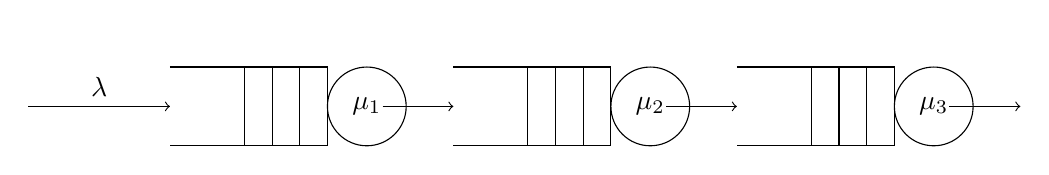
\begin{tikzpicture}[xscale=0.9,
->-/.style={decoration={markings, mark=at position .5 with {\arrow{stealth}}},
postaction={decorate}},
queuei/.pic={
  \draw%[line width=1pt]
    (0,-0.5) -- ++(2cm,0) -- ++(0,-1cm) -- ++(-2cm,0);
   \foreach \Val in {1,...,3}
     \draw ([xshift=-\Val*10pt]2cm,-0.5) -- ++(0,-1cm);
\draw (2.5,-1) circle [radius=0.5cm] node {#1};}
]
\path 
  (0,1) pic {queuei=$\mu_1$}
  (4,1) pic {queuei=$\mu_2$}
  (8,1) pic {queuei=$\mu_3$};

\draw[->] (-2,0)--(0,0) node[midway, anchor=south] {$\lambda$};
\draw[->] (3,0)--(4,0); 
\draw[->] (7,0)--(8,0); 
\draw[->] (11,0)--(12,0); 
%\draw[->-] (2.5,-0.5)-- ++(0,-1) -- ++(5.,0) -- ++(0, 1.5); 

\end{tikzpicture}

  \begin{solution} 
    The raw processing time is just the sum of the processing times at
    each station. All stations have the same arrival rate, hence
    machine, being the slowest, is the bottleneck. Hence,
 \begin{align*}
      T_0 &= 2 + 3 + 2 = 7\\
   r_b &= \mu_2 = \frac13 \\
      W_0 &= r_b T_0 = \frac73.
    \end{align*}
  \end{solution}
\end{exercise}

\begin{exercise}
  A production network consists of 3 single-machine stations in tandem
  with processing times $(2, 3, 2)$ hours.  Suppose we modify this
  network by adding one extra machine to station 2, with processing
  time $t=3$ hours.  What are $W_0$, $r_b$ and $T_0$?
  \begin{hint}
Is the new machine placed in parallel or in series?
  \end{hint}
  \begin{solution}
    Realize that machines at a station are in parallel, not in
    series. Thus, when we add capacity to station 2, we don't add an
    extra processing step to station 2, we increase capacity. 

    Now 
    \begin{equation*}
      r_2 = \frac13 + \frac13 = \frac 23,
    \end{equation*}
    so that station 2 is no longer the bottleneck. Station 1 and
    station 3 are the bottlenecks.
    \begin{align*}
      r_b &= \frac12 \\
      T_0 &= 2 + 3 + 2 = 7\\
      W_0 &= r_b T_0 = \frac72.
    \end{align*}

    Often, students think that the processing rate is the inverse of
    the processing time, i.e., $t=r^{-1}$. This is not the case for
    multi-server stations. Thus, realize that the raw processing time
    at station 2 is still $3$ hours, not $3/2$.
  \end{solution}
\end{exercise}


\begin{exercise}
  A production network consists of 3 single-machine stations in tandem
  with processing times $(2, 3, 2)$ hours.  Suppose we modify this
  network by adding one extra machine to station 2 with
  processing time $t=4$ hours.  What are $W_0$, $r_b$ and $T_0$?
  \begin{hint}
Check your reasoning very carefully here. It is easy to do it wrong.
  \end{hint}
\begin{solution}
Now, 
\begin{equation*}
  r_2 = \frac13 + \frac 14 = \frac 7{12} > \frac12,
\end{equation*}
hence, station 1 and 3 are bottlenecks. 


However, $t_2$ cannot be $3$ hours anymore: some jobs will spend 4
hours at station 2 rather than 3 hours. In fact, the computation of
the raw processing time at station 2, $t_2$ say, is a bit tricky. Some
students reason that both machines serve half of the jobs, so that
$T_2=(3+4)/2$ hours.  This, however, is not quite realistic. Like
this, you would load the slow machine all of the time, and the faster
machine would be idle quite a bit of the time. 


  Rather than spreading the jobs evenly over the two machines, we can
  also assume that each machine takes in work in proportion to its
  processing rate.  Then we reason like this. Consider 12 hours. In
  those 12 hours, the slow machine processes 3 jobs with duration 4
  and the fast machine processes 4 jobs with duration 3. Therefore:
  \begin{equation*}
    t_2 = \frac 3 7 4 + \frac 4 7 3 = \frac{24}7.
  \end{equation*}
  Another way to get this is like this. We can `stuff' station 2 with
  jobs. The most jobs that fit in simultaneously is 2, one job per
  machine. Then, with Little's law,
  \begin{equation*}
   t_2 = \frac{W}{r_2} = \frac{2}{7/12} = \frac{24}7,
  \end{equation*}
i.e., the same as the other answer.

Now, finally, 
    \begin{align*}
      r_b &= \frac12 \\
      T_0 &= 2 + \frac{24}7 + 2 = 4 + 3 + \frac37 = 7 \frac37\\
      W_0 &= r_b T_0.
    \end{align*}

    Finally, and the most realistic, is that the fast machine is
    always working, and the slow machine covers the rest.  In that
    case, suppose that the fast machine processes jobs at rate $r_1$
    and the slow at rate $r_2$. Then, since jobs arrive with rate
    $r_a$, the fast machine processes a fraction of $r_1/r_a$ of the
    jobs, and the slow machine processes the left overs, i.e., a
    fraction of $(r_a-r_1)/r_a$ of the jobs. The raw processing time then becomes
    \begin{equation*}
      \begin{split}
      t_2 
&= \frac{r_1}{r_a} t_1 + \frac{r_a-r_1}{r_a} t_2 \\
&= \frac{1/3}{1/2} 3 + \frac{1/2-1/3}{1/2} 4 \\
&= 2 + \frac{1/6}{1/2} 4 \\
&= 2 + \frac{4}{3} = 3\frac13,
      \end{split}
    \end{equation*}
and then,
\begin{equation*}
  T_0 = 2 + t_2 + 2 = 7\frac13,
\end{equation*}
and this is a tiny bit less then the previous way of organizing things. 

So, why are the above answers different? One reason is that the
objective is not explicitly stated. It might be that, to minimize time
in a multi-server station, it is optimal to let a fast machine idle
and wait until the next job comes in. If we were to assign this next
job to a slow machine, the time in the system may be longer.  In
general, it might be that schedules that minimize $T_0$ (on average)
are not work-conserving (i.e., such that when jobs are waiting, not
all machines are idle.)
\end{solution}
\end{exercise}


\begin{exercise}
Why does the critical WIP change in the different cases above? 
\begin{solution}
  Because $T_0$ increases and/or the bottleneck rate increases. In
  both cases, we need more $W_0$ to fill the network and achieve that
  the throughput can be equal to $r_b$ in the best case.
\end{solution}
\end{exercise}

\begin{exercise}
  A production network consists of 3 single-machine stations in tandem
  with processing times $(2, 3, 2)$ hours.  Suppose we modify this
  network by adding one extra machine to station 2 with 
  processing time $t=1$ hour.  What are $W_0$, $r_b$ and $T_0$?
\begin{solution}
  Now the slow machine at station 2 becomes superfluous. The fast
  machine at station 2 can cope with all jobs that arrive from station
  1.
    \begin{align*}
      r_b &= \frac12 \\
      T_0 &= 2 + 1 + 2 = 5\\
      W_0 &= r_b T_0.
    \end{align*}

    Thus, why would you assign part of the jobs to the slow machine at
    station 2? There is no queue, the fast machine can cope with all
    the jobs. Moreover, assigning any job to the slow machines just
    adds to the cycle time.

Taking  $T_2=(1+3)/2=2$ is plainly silly. 
\end{solution}
\end{exercise}

\begin{exercise}
  In the previous question, it might seem that one machine at the
  second station is superfluous. Which one, and why? Would you remove
  this superfluous machine in a real production network?
\begin{solution}
  See above. I would not remove the slow machine. In real life there
  is variability: the fast machine might fail for instance. Spare
  capacity is useful. However, if it is very costly to keep the slow
  machine operational, I would scrap it.
\end{solution}
\end{exercise}


% What would you have
% said if the processing time of the slow machine would have been 5
% hours? Then you simply cannot give half of the jobs to the slow
% machine; it will overflow.

\begin{exercise}
  A production network consists of 3 single-machine stations in tandem
  with processing times $(2, 3, 2)$ hours.  Suppose we modify this
  network by adding one extra machine to station 2 with processing
  time $t=7$ hours.  What are $W_0$, $r_b$ and $T_0$?
\begin{solution}
  \begin{align*}
  r_2 &= \frac13 + \frac17 = \frac{10}{21} < \frac12\\
\intertext{hence station 2 is still the bottleneck}
T_2 &= \frac{3}{10}7 + \frac{7}{10}3 = \frac{42}{10}=\frac{21}{5}\text{hour}\\
T_0&=2+\frac{21}{5} +2\\
r_b &= \frac{10}{21}\\
W_0 &= r_b T_0.
   \end{align*}

   Note that we add capacity, so that we can process more jobs per
   unit time, but the raw processing time increases!
\end{solution}
\end{exercise}


\begin{exercise}
  A production network consists of 3 single-machine stations in tandem
  with processing times $(2, 3, 2)$ hours.  Suppose we modify this
  network such that $2/3$ of the jobs \emph{ leave after the first}
  station, i.e., between station 1 and 2.  What are $W_0$, $r_b$ and
  $T_0$? 
\begin{solution}
  Now there are two loops. One third of the jobs pass all three
  stations. Station 1 can process these job at rate 
  \begin{equation*}
\frac13 r_1 = \frac 13 \frac 12=\frac 16
  \end{equation*}
  per hour. Since this is smaller than $r_2$ and $r_3$, station 1 is
  the bottleneck rate for this loop. Thus, $W_0$ in this loop is
  $r_b T_0 = 1/6\cdot 7 = 7/6$.

  The other loop only contains station 1. The bottleneck rate in this
  loop is 
  \begin{equation*}
r_1\frac23 = \frac12\frac23 = \frac13. 
  \end{equation*}
Thus,
  $W_0 = r_b T_0 = 1/3\cdot 2 = 2/3$ for this loop. 

Hence, the total WIP is $7/6 + 2/3 = 11/6$ and
\begin{equation*}
T_0 = \frac13  7 + \frac 23  2=\frac{11}3,
\end{equation*}
since $1/3$ take the long loop with $T=7$ and $2/3$ the short loop
with $T=2$. Thus, $T_0$ is the weighted average raw processing time.

Another way to analyze this situation is like this. Station 1 is the
bottleneck, because its utilization is 1, while
\begin{align*}
  \rho_2 &= \lambda_2 t_2 = \frac12\frac13 3 = \frac 12\\
  \rho_3 &= \lambda_3 t_3 = \frac12\frac13 2 = \frac 13.
\end{align*}
Since station 1 is the bottleneck in this network, $r_b=1/2$. Since
$T_0 = 11/3$, which we obtain as the weighted average computation
above, we must have that 
\begin{equation*}
W_0 = r_b T_0 = \frac12\frac{11}3 = \frac{11}6, 
\end{equation*}
which agrees with our earlier result.
\end{solution}
\end{exercise}


\begin{exercise}
  A production network consists of 3 single-machine stations in tandem
  with processing times $(2, 3, 2)$ hours.  Suppose we modify this
  network such that 4/5 of the jobs \emph{bypass the second} station,
  i.e., 1/5 of the jobs have the routing $[1,2,3]$, but 4/5 have
  routing $[1,3]$.  What are $W_0$, $r_b$ and $T_0$?
\begin{solution}
  Now stations 1 and 3 are bottlenecks with $r_b = 1/2$. For $T_0$ we have
  \begin{equation*}
    T_0 = \frac15 7 + \frac45 4= \frac{23}5.
  \end{equation*}
Thus, 
\begin{equation*}
W_0 = r_b T_0 = \frac 12 \frac{23}5 = \frac{23}{10}.
\end{equation*}
\end{solution}
\end{exercise}

% \begin{exercise}
%   Building up on the previous question, which stations would you
%   include anyway in a CONWIP loop, and why?
% \end{exercise}
% \begin{solution}
%   Now stations 1 and 3 are bottleneck. Thus, both stations need to be
%   part of the conwip loop. For that matter, it is just as easy to also
%   include station 2, and just include all work on the floor in the WIP
%   measurements.
% \end{solution}


Production situations can be pretty  complicated. Jobs can enter the network at different places, not  just at station 1 as we considered here. Jobs may also need rework  at one or more stations. One consequence of these aspects is that   the slowest machines or stations need not be the bottlenecks. If you like, you can try to find or develop a general algorithm to compute
 $T_0$, $W_0$ and $r_b$ for any network of reasonable size.  One way to approach this problem might be to  place (imaginary) huge  amounts of work in front of each station and just see how the network drains, another is to try to find an analogy with an electrical network. All in all, its an elegant  problem.

\Closesolutionfile{hint}
\Closesolutionfile{ans}

\opt{solutionfiles}{
\subsection*{Hints}
\input{hint}
\subsection*{Solutions}
\input{ans}
}

%\clearpage


%%% Local Variables:
%%% mode: latex
%%% TeX-master: "../queueing_book"
%%% End:

% \section{Open Single-Class Product-Form Networks}
\label{sec:jackson-networks}


\subsection*{Theory and Exercises}

\Opensolutionfile{hint}
\Opensolutionfile{ans}

The remark above Zijm.Eq.2.11 is not entirely correct. Remove the
sentence: `These visit ratios satisfy \ldots up to a multiplicative
constant'.


I don't like the derivation of Zijm.Eq.2.20. The appearance of the
visit ratios $\lambda_i/\gamma$ seem to come out of thin air. The
argument should be like this. Consider the entire queueing network as
one `box' in which jobs enter at rate $\gamma=\sum_{i=1}^M
\gamma_i$.
Assuming that there is sufficient capacity at each station, i.e.,
$\lambda_i < c_i \mu_i$ at each station $i$, the output rate of the `box' must also be $\gamma$. Thus, by applying Little's law to the `box', we have that 
\begin{equation*}
  \E L = \gamma \E W. 
\end{equation*}
It is also evident that the average total number of jobs must be equal
to the sum of the average number of  jobs at each station: 
\begin{equation*}
  \E L = \sum_{i=1}^M \E{L_i}.
\end{equation*}
Applying Little's law to each station separately we get that
$\E{L_i} = \lambda_i\E{W_i}$. Filling this into the above,
\begin{equation*}
\E W = \frac{\E L}{\gamma}  = \sum_{i=1}^M \frac{\E{L_i}}\gamma = \sum_{i=1}^M \frac{\lambda_i \E{ W_i}}\gamma, 
\end{equation*}
where we recognize the visit ratios.




\begin{comment}
\begin{exercise}[use=false]
  Use the ideas of Zijm.Eq.2.2 to set up a set of balance equations
  for a single-server queueing station with two queues such that queue
  1 is served with strict priority over queue 2, and service of a job
  of type 2 is preemptive. Assume that type i jobs arrive at rate
  $\lambda_i$ and require average service time
  $\mu_i^{-1}$. Inter-arrival times of jobs each type are exponentially distributed,
  just as the service times.

  Can you find similar equations for the case with multiple servers at
  the station, all serving type 1 jobs with strict priority over type
  2 jobs?
  \begin{solution}
    TBD.
  \end{solution}
\end{exercise}
  
\end{comment}

\begin{exercise}(Linear algebra refresher) Can you find an example to
  show for two matrices $A$ and $B$ that $AB\neq BA$, hence
  $x A \neq A x$.
  \begin{hint}
    Let 
    \begin{equation*}
A =
    \begin{pmatrix}
      1 & 1 \\ 
0&1
    \end{pmatrix},
\quad   B=
    \begin{pmatrix}
      1 & 0 \\ 
1&1
    \end{pmatrix}
    \end{equation*}.
  \end{hint}

  \begin{solution}
    \begin{equation*}
      AB =  
    \begin{pmatrix}
      2 & 1 \\ 
1&1
    \end{pmatrix} 
\neq
    \begin{pmatrix}
      1 & 1 \\ 
1&2
    \end{pmatrix} 
= BA.
    \end{equation*}

Take $x=(1,1)$, then $x A=(1,2)$. Now, taking $x=
\begin{pmatrix}
  1 \\
1
\end{pmatrix}
$, we get $Ax = 
\begin{pmatrix}
  2 \\
1
\end{pmatrix}.  $
Recall, horizontal vectors are not vertical vectors. The horizontal
ones are to the left of a matrix, and the vertical ones to the right.
  \end{solution}
\end{exercise}

\begin{exercise}(Linear algebra refresher, 2) Suppose the matrix $A$
  has an eigenvalue $0$. What is the geometric meaning of this fact? 
  \begin{solution}
    Many students think that a matrix is just a bunch of numbers
    ordered in a grid. This is, in my opinion, the most unproductive
    way to think about matrices. A much more useful way is to see a
    matrix as an \emph{operator}. For instance, take $A$ to be a
    $3\times3$ matrix. Then it can be seen as \emph{mapping} from
    $\R^3$ to $\R^3$; it takes a vector $x\in\R^3$ and changes $x$
    into a new vector $Ax\in \R^3$. Thus, a square matrix $A$ typically changes the
 direction of a vector $x$. 

With this idea, consider the simple example with
    \begin{equation*}
A =
    \begin{pmatrix}
      1 & 0 & 0 \\ 
      0 & 1 & 0 \\ 
      0 & 0 & 0 \\ 
    \end{pmatrix}.
  \end{equation*}
Clearly, $A$ has an eigenvalue $0$. Now take $v=(x,y,z)'$, so that
    \begin{equation*}
A v = A
 \begin{pmatrix}
x\\
y\\
z
    \end{pmatrix}
= \begin{pmatrix}
x\\
y\\
0
    \end{pmatrix}.
  \end{equation*}
  We see that $A$ removes any information about the $z$ direction from
  the vector $v$. (It projects $v$ on the $x-y$ plane, and throws away
  the $z$ component of $v$.) But then, for a given vector $w=(x,y,0)$
  in the $x-y$ plane, it is impossible to use $A$ to retrieve the
  original vector $v=(x,y,z)$. Thus, $A$ cannot have an inverse on all
  of $\R^3$.

  So, hopefully, with this example, you can memorize that for any
  matrix $A$ to have an inverse, it is essential that it has no zero
  eigenvalues. When the \emph{operator} $A$ (don't think of a matrix
  as a set of numbers) throws away part of the dimension of the space
  on which it operates (i.e., it has one or more eigenvalue(s) $0$), it is impossible to retrieve the part of the space it throws away. Hence, its inverse cannot be used to get this part of the space back. 

\end{solution}


\end{exercise}


\begin{exercise}
Zijm.Ex.2.2.1
\begin{solution}
Because jobs cannot leave faster than they arrive.
\end{solution}
\end{exercise}

\begin{exercise}
Zijm.Ex.2.2.2
\begin{solution}
  Observe from Exercise~\ref{ex:dep} that the inter-departure times
  of the $M/M/1$ queue are also independent and identically
  exponentially distributed with rate $\lambda$. Since the arrival
  process at the second station is the departure process of the first
  station, it must be that arrival process at the second station is
  also Poisson with rate $\lambda$.  Interestingly, from the
  perspective of the second station it is as if there is not first
  station.
\end{solution}
\end{exercise}



\begin{exercise}
Zijm.Ex.2.2.3 
\begin{solution}
  The question is not well specified. We know from Burke's law, see Exercise~\ref{ex:burke}, that
  the arrival \emph{process} at the second station is Poisson.  If,
  however, we know that station 1 is empty, then it is unlikely that a
  job will arrive at station 2 in the very near future.

  Note that only the steady-state distributions of the queue lengths
  are independent. Once you have information about the state of one of
  the queues, then certainly this is not in `steady-state'.
\end{solution}
\end{exercise}

\begin{exercise}
Zijm.Ex.2.2.4
\begin{solution}
  Simple algebra.  (I am not going to write it out here. If you are
  willing to provide me the answer in \LaTeX\/ I'll include it.)
\end{solution}
\end{exercise}

\begin{exercise}
  Zijm.Ex.2.2.5. The problem is not entirely correctly formulated. It
  should be, if for at least one $i$, $\sum_{j=1}^M P_{i j} <1$ \ldots
\begin{solution}
Linear algebra is quite useful here!

Observe that $P_{i j}$ is the probability that a job, after completing
its service at node $i$, moves to node $j$. Then $\sum_{j=1}^M P_{i j}$
is the probability that a job moves from node $i$ to another node in
the network, i.e., stays in the network, while $P_{i0}$ is the
probability that a job departing from node $i$ leaves the network, in
other words, the job is finished. When $\sum_{j=1}^M P_{i j} < 1$, then
more jobs enter node $i$ from the network than that node $i$ sends
`back' into the network. Conceptually, node $i$ `leaks jobs'.

  Now, consider some node $k$ such that $P_{ki} > 0$, then the
  probability that a job that starts at node $k$, moves to node $i$
  and then leaves the network is equal to $P_{ki}P{i0}$. Thus, since
  $P_{ki}>0$ and $P_{i0}>0$, the probability that a job leaves the
  network from note $k$ in two steps is positive.  More specifically,
  $P^2_{k0} = \sum_{j=0}^M P_{kj}P_{j0} \geq P_{ki}P_{i0} > 0$. 

  The irreducibility assumption implies that in at most $M$ steps it
  is possible to reach, with positive probability, any node from any
  other node in the network. Thus, for any node $j$ to any other node
  $k$ there is a sequence of nodes $j_1, j_2, \ldots j_{M-1}$ such
  that  $P^{M}_{jk} \geq P_{j j_1}P_{j_1 j_2}\cdots P_{j_{M-1}k} > 0$.


  Thus, if there is a node $i$ such that $P_{i0}>0$, then it is
  possible from any node that sends jobs to node $i$ directly to leave
  the network in two steps. Likewise, when node $i$ can be reached
  from node $k$ in $n$ steps, say, then
  $P^{n+1}_{k0} \geq P^n_{ki}P_{i0} > 0$, i.e., in at most $n+1$ steps
  it is possible to leave the network from such node $k$. This
  implies, in particular, that for all nodes $k=1,2,\ldots M$, i.e.,
  all nodes in the network, $P^{M+1}_{k0} >0$.  For this reason we
  consider $P^{M+1}$ in the hint.


  As a final remark for students with knowledge of Markov chains,
  observe that the routing matrix $P$ does not correspond to the
  transition matrix of a recurrent Markov chain. Since for at least
  one row $i$, $\sum_{j=1}^N P_{i j}<1$, the matrix $P$ is
  sub-stochastic. Hence, a Markov chain induced by $P$ cannot be
  irreducible, because for this to happen, the chain must stay in some
  absorbing set with probability 1.
\end{solution}
\end{exercise}

\begin{exercise}
Zijm.Ex.2.2.6
\begin{solution}
  Since $M$ is finite, and $k\leq M$, the set of numbers
  $P^{M+1}_{k0}$ is finite. This, together with the fact that
  $P^{M+1}_{k0}>0$ for all $k$, implies that there is some number
  $\epsilon>0$ such that $P^{M+1}_{k0}>\epsilon$. Hence, for all
  entries $k=1, 2, \ldots M$, we have that
  $P^{M+1}_{kj} < 1- \epsilon$. This, in turn, implies that
  $P^{2(M+1)}_{kj} < (1- \epsilon)^2$, and so on, so that for any $n$,
  $P^{n(M+1)}_{kj} < (1- \epsilon)^n$. This implies, in more general
  terms, that the entries of $P^n$ decrease at some geometric rate to
  $0$.

  It is well known that for any bounded sequence $x_i$ and
  $0\leq \alpha < 1$, $ \sum_{i=0}^\infty x_i \alpha^i <
  \infty$. Applying this insight to the entries of $P^n$ it follows that 
$\sum_{n=0}^\infty P^n_{jk} < \infty$. 

Finally, applying  $\lambda = \gamma + \lambda P$ recursively, we get
\begin{equation*}
  \lambda = \gamma + \lambda P = \gamma + (\gamma + \lambda P)P = \gamma (1+P) + \lambda P^2 = \gamma(1+P+P^2) + \lambda P^3 \to \gamma \sum_{n=0}^\infty P^n.
\end{equation*}
By the above reasoning this last sum is well defined, and finite.  (By
the way, the above argument is not necessarily valid for matrices $P$
that are infinite, since then $\inf\{P^{M}_{ik}\}$ need not be
strictly positive.)

Another interesting way to see all this is by making the simplifying
assumption that $P$ is a diagonalizable matrix. (The argument can be
generalized to include matrices reduced to Jordan normal form, but
this gives optimal clutter, but does not change the line of reasoning in
any fundamental way.) In that case, there exists an invertible matrix
$V$ with the (left) eigenvectors of $P$ as its rows and a diagonal
matrix $\Lambda$ with the eigenvalues on its diagonal such that
\begin{equation*}
  V P = \Lambda V.
\end{equation*}
Hence, premultiplying with $V^{-1}$, 
\begin{equation*}
  P = V^{-1}\Lambda V.
\end{equation*}
But then
\begin{equation*}
P^2 = V^{-1}\Lambda V \cdot V^{-1}\Lambda V= V^{-1}\Lambda^2 V,
\end{equation*}
and in general $P^n = V^{-1}\Lambda^n V$. If each eigenvalue
$\lambda_i$ is such that its modulus $|\lambda_i| < 1$, then
$\Lambda^n \to 0$ geometrically fast, hence $P^n\to n$ geometrically
fast, hence the sequence of partial sums $\sum_{n=0}^N P^n$ must
converge to some finite number as $N\to\infty$. 

So, we are left with proving that the eigenvalues of $P$ must have
modulus less than $1$. This fact follows from Gerschgorin's disk
theorem, which I include for the interested student. Define the disk
$B(a,r)=\{z\in \mathbb{C} | |z-a|\leq r\}$, i.e., the set of complex numbers
such that the distance to the center $a\in \mathbb{C} $ is less than or equal
to the radius $r$. With this, the Gerschgorin disks of a matrix are
defined as $B(a_{ii}, \sum_{j\neq i} |a_{i j}|)$, i.e., disks with
center at the diagonal elements $a_{ii}$ of $A$ and and radius equal
to the sum of the (modulus of the) elements of $A$ on the $i$th row
except $a_{ii}$. Then Gerschgorin's theorem says that all eigenvalues
of $A$ lie in the union of these disks, i.e., all eigenvalues
$\lambda_i \in \bigcup_i B_{a_{ii}, \sum_{j\neq i}|a_{i j}})$.

Assume for notational simplicity that for each row $i$ of $P$ we have
that $\sum_{j} a_{i j}<1$. (Otherwise apply the argument to $P^{M+1}$.)
Then this implies for all $i$ that
\begin{equation*}
  a_{ii} + \sum_{j\neq i} a_{i j} < 1. 
\end{equation*}
Since all elements of $P$ are non-negative, this also implies that
\begin{equation*}
-1 <   a_{ii} - \sum_{j\neq i} a_{i j} \leq  a_{ii} + \sum_{j\neq i} a_{i j} < 1. 
\end{equation*}
With this and using that $a_{ii}$ is a real number (so that it lies on
the real number axis) it follows that all elements in the disk
$B(a_{ii}, \sum_{j\neq i} a_{i j})$ have modulus smaller than 1.  As
this applies to any row $i$, all disks lie strictly within the complex
unit circle. But then, by Gerschgorin's theorem, all eigenvalues of
$P$ also lie strictly in the unit circle, hence all eigenvalues have
modulus smaller than 1.
\end{solution}
\end{exercise}

\begin{exercise}\label{ex:23}
  Show that Zijm.Eq.2.13 and 2.14 can be written as
  \begin{equation*}
    f_i(n_i) = \frac{1}{G(i)}\frac{1}{\Pi_{k=1}^{n_i} \min\{k, c_i\}}\left( \frac{\lambda_i}{\mu_i}\right)^{n_i}.
  \end{equation*}
  \begin{solution}
    Take $n_i<c_i$. Then
    $\Pi_{k=1}^{n_i} \min\{k, c_i\} = \Pi_{k=1}^{n_i} k = n_i!$, and
    $(c_i\rho_i)^{n_i} = (\lambda_i/\mu_i)^{n_i}.$ If $n_i\geq c_i$,
    then $\Pi_{k=1}^{n_i} \min\{k, c_i\} = c_i! c_i^{n_i-c_i}$, and
    $(c_i\rho_i)^{n_i} = (\lambda_i/\mu_i)^{n_i} c_i^{n_i}.$.
  \end{solution}
\end{exercise}


\begin{exercise}
Zijm.Ex.2.2.7
\begin{solution}
  \begin{equation*}
    P = 
    \begin{pmatrix}
      \alpha & 1- \alpha \\
      \beta_1 & \beta_2
    \end{pmatrix}.
  \end{equation*}

  \begin{equation*}
    (\lambda_1, \lambda_2) = (\gamma, 0) + (\lambda_1, \lambda_2) P.
  \end{equation*}
Solving first for $\lambda_2$ leads to $\lambda_2 = (1-\alpha) \lambda_1 + \beta_2 \lambda_2$, so that  
\begin{equation*}
  \lambda_2 = \frac{1-\alpha}{1-\beta_2} \lambda_1. 
\end{equation*}
Next, using this and that $\lambda_1 = \alpha \lambda_1 + \beta_1 \lambda_2 + \gamma$ gives with a bit of algebra
\begin{equation*}
  \begin{split}
\gamma 
&=  \lambda_1(1-\alpha) - \beta_1\lambda_2 \\
&=  \lambda_1\left(1-\alpha - \beta_1\frac{1-\alpha}{1-\beta_2}\right) \\
&=  \lambda_1(1-\alpha)\left(1 - \frac{\beta_1 }{1-\beta_2}\right) \\
&=  \lambda_1(1-\alpha)\frac{1-\beta_1-\beta_2 }{1-\beta_2}.
  \end{split}
\end{equation*}
Hence, 
\begin{equation*}
  \lambda_1 = \frac\gamma{1-\alpha}\frac{1-\beta_2}{1-\beta_1-\beta_2}. 
\end{equation*}
Thus, 
\begin{equation*}
  \lambda_2 = \frac{1-\alpha}{1-\beta_2} \lambda_1 = \frac\gamma{1-\beta_1-\beta_2}. 
\end{equation*}


We want of course that $\lambda_1 < \mu_1$ and $\lambda_2 < \mu_2$.
With the above expressions this leads to conditions on $\alpha$,
$\beta_1$ and $\beta_2$. Note that we have three parameters, and two
equations; there is not a single condition from which the stability
can be guaranteed.

If $\alpha\uparrow 1$, the arrival rate at node $1$ explodes. If
$\beta_1=0$ no jobs are sent from node 2 to node 1.

\end{solution}
\end{exercise}
\begin{exercise}
Zijm.Ex.2.2.8
\begin{solution}
  Yes, the network remains a Jackson network. By Burke's law, see Exercise~\ref{ex:burke}, the
  departure process of each node is Poisson. In one of the earlier
  questions we derived that splitting (also known as thinning) and
  merging Poisson streams again lead to Poisson streams. The
  departures from node $j$ to node $k$ forms a thinned Poisson
  stream. The external arrivals plus internal arrivals are merged into
  one Poisson stream, hence the arrivals at a station also form a Poisson stream.

  Observe that the exponentiality of the service times and external
  inter-arrival times and Burke's law are essential for the argument.
\end{solution}
\end{exercise}

\begin{exercise}
  (Hall 5.22). At a large hotel, taxi cabs arrive at a rate of 15 per
  hour, and parties of riders arrive at the rate of 12 per
  hour. Whenever taxicabs are waiting, riders are served immediately
  upon arrival. Whenever riders are waiting, taxicabs are loaded
  immediately upon arrival. A maximum of three cabs can wait at a time (other cabs must go elsewhere).
  \begin{enumerate}
  \item Let $p_{ij}$ be the steady-state probability of there being $i$ parties of riders and $j$ taxicabs waiting at the hotel. Write the state transition equation for the system. 
  \item Calculate the expected number of cabs waiting and the expected number of parties waiting.
  \item Calculate the expected waiting time for cabs and the expected waiting for parties. (For cabs, compute the average among those that do not go elsewhere.)
  \item In words, what would be the impact of allowing four cabs to wait at a time?
  \end{enumerate}
  \begin{hint}
This is really a neat problem. Please spend serious time on it to
solve before looking at the answer. It requires some ingenuity on your part.  Try to adapt the ideas behind Figure 2.2 of Zijm to this case.
  \end{hint}
    \begin{solution}
Let $p_{ij}$ be the fraction of time that the system contains $i$
riders and $j$ taxi cabs. I assume that all members of a party of
riders can be served by a single cab (that is, the parties do not
exceed the capacity of a cab and all members of a party have the same
destination). For clarity, write $\mu$ for the rate at which cabs
arrive, and $\lambda$ for the arrival rate of parties of riders.  Then
the transitions are as in the figure below. Suppose first that there
are $3$ taxi cabs. When a group arrives (at rate $\lambda$), there is
one taxi less, and so on, until there are no more taxi's
left. Finally, if yet more groups arrive, they have to wait. When a
new taxi arrives, the number of groups is reduced by one, and so on,
until there are $3$ taxi's waiting and no groups of people.


    \begin{center}

\begin{tikzpicture}[->,>=stealth',shorten >=1pt,auto,node distance=1.8cm,
                    semithick]
  \node[state] (0) {$p(0,3)$} ;
  \node[state] (1) [right of=0] {$p(0,2)$};
  \node[state] (2) [right of=1] {$p(0,1)$};
  \node[state] (3) [right of=2] {$p(0,0)$};
  \node[state] (4) [right of=3] {$p(1,0)$};
  \node[state] (5) [right of=4] {$p(2,0)$};
  \node[state] (6) [right of=5] {$p(\cdot, 0)$};

\path 
 (0) edge [bend left] node {$\lambda$} (1)
 (1) edge [bend left] node {$\mu$} (0)
 (1) edge [bend left] node {$\lambda$} (2)
 (2) edge [bend left] node {$\mu$} (1)
 (2) edge [bend left] node {$\lambda$} (3)
 (3) edge [bend left] node {$\mu$} (2)
 (3) edge [bend left] node {$\lambda$} (4)
 (4) edge [bend left] node {$\mu$} (3)
 (4) edge [bend left] node {$\lambda$} (5)
 (5) edge [bend left] node {$\mu$} (4)
 (5) edge [bend left] node {$\lambda$} (6)
 (6) edge [bend left] node {$\mu$} (5)
;
\end{tikzpicture}
      
    \end{center}

From this figure, we see that
\begin{align*}
\lambda p_{0,3} &= \mu p_{0,2} \\
(\lambda+\mu) p_{0,2} &= \mu p_{0,1} + \lambda p_{0,3}\\
(\lambda+\mu) p_{0,1} &= \mu p_{0,0} + \lambda p_{0,2}\\
(\lambda+\mu) p_{0,0} &= \mu p_{1,0} + \lambda p_{0,1}\\
(\lambda+\mu) p_{1,0} &= \mu p_{2,0} + \lambda p_{0,0}\\
(\lambda+\mu) p_{2,0} &= \mu p_{3,0} + \lambda p_{1,0}\\
\end{align*}
And so on. Thus, it is left to compute $p_{ij}$. Observe from this
scheme, or the above figure, that the situation with the taxi's
correspond to an $M/M/1$ queue, only the states have a `different
name'. Let $q$ be the number of jobs in an M/M/1 queue. Some thought
will reveal that the queueing system with cabs and parties can be
mapped to an equivalent M/M/1 queueing system. In fact, consider the
following table
\begin{center}
\begin{tabular}{ccc}
$j$ & $i$ & $q$\\
3&         0 &         0\\
2 &        0&          1\\
1 &        0&          2\\
0&         0&          3\\
0&         1&          4\\
0&         2&          5\\
\end{tabular}
\end{center}
and so on. Therefore, in general, it must be that 

\begin{equation*}
q = 3 - j +i.
\end{equation*}
From the M/M/1 queue we know right away that $p_q = \rho^q
(1-\rho)$.  With the above relation we can therefore immediately find
that $p_{ij} = \rho^{3-j+i}(1-\rho)$, save that $i$ and
$j$ must satisfy the constraints imposed by the model.

Second, the expected number of cabs waiting must be 
\begin{equation*}
1p_{0,1} + 2 p_{0,2} + 3p_{0,3}
\end{equation*}
and the expected number of parties waiting must be $\sum_{j=1}^\infty j p_{j,0}$

\begin{pyconsole}
labda = 12. # per hour
mu = 15. # per hour
rho = labda/mu

def p(i,j):
    q  = 3 - j + i
    return rho**q*(1.-rho)

\end{pyconsole}
Expected number of  cabs waiting:
\begin{pyconsole}
Lc = sum(j*p(0,j) for j in range(0,4)) 
# Recall this sums up to 4, not including 4
Lc
  
\end{pyconsole}


To compute the expected number of parties waiting we formally have to
sum to infinity. Rather than doing the algebra, I chose to truncate
the summation at an $i$ such that $\rho^i \ll 1$, i.e.,
negligible.  Truncating at 30 seems reasonable enough:

\begin{pyconsole}
trunc = 30
rho**trunc
\end{pyconsole}

At second thought this is not yet really small. 

\begin{pyconsole}
trunc = 50
rho**trunc
\end{pyconsole}


This is better. Now go for what we want to know:

\begin{pyconsole}
Lp = sum(i*p(i,0) for i in range(trunc))
Lp
\end{pyconsole}

For the last part: This is tricky. I first, naively, computed $W_q = L_c/\mu$. This
seems to make sense, as cabs arrive at rate $\mu$, so that this
expression follows from a standard application of Little's
law. However, this is wrong, of course. When using Little's law to
relate the number of jobs in queue (i.e., in the M/M/1 queue) and the
queueing time we need to use $\lambda$, not
$\mu$. Similarly (and more formally by the mapping developed in
part a), for our cab system we also need to use $\lambda$.

\begin{pyconsole}
Wq = Lc/labda
Wq
\end{pyconsole}

Thinking in templates is often useful, but makes one sloppy\ldots

What would be the impact of allowing 4 cabs? Funny question, and with the above, trivial to answer.

\begin{pyconsole}
def p(i,j):
    q  = 4 - j + i
    return rho**q*(1.-rho)
  
\end{pyconsole}

\begin{pyconsole}
Lc = sum(j*p(0,j) for j in range(0,4))
Lc

Lp = sum(i*p(i,0) for i in range(trunc))
Lp
  
\end{pyconsole}
    \end{solution}
\end{exercise}



\begin{comment}
  
\begin{exercise}[use=false]
  Include an question that shows that it is necessary to check the
  guess for the product form solution everywhere on the state space,
  that is, in the interior, but also on the boundaries.
  \begin{solution}
    TBD
  \end{solution}
\end{exercise}

\begin{exercise}[use=false]
  Apply the formula's of Zijm.Section 2.4 to a tandem queueing network.
  \begin{solution}
    TBD.
  \end{solution}
\end{exercise}

\begin{exercise}[use=false]
  Include a case for Section 2.4.
  \begin{solution}
    TBD.
  \end{solution}
\end{exercise}
\end{comment}


\Closesolutionfile{hint}
\Closesolutionfile{ans}

\opt{solutionfiles}{
\subsection*{Hints}
\input{hint}
\subsection*{Solutions}
\input{ans}
}
%\clearpage



%%% Local Variables:
%%% mode: latex
%%% TeX-master: "../queueing_book"
%%% End:

% 
\section{Tandem queues}
\label{sec:tandem-queues}

No notes; only exercises.

\begin{question}
  Consider two stations in tandem. The service process at both
  stations is subject to variability. Suppose you have some money to
  spend on reducing the variability of either of the two machines.
  Which one is the better one to spend it on?  You should realize the
  relevancy of modeling for this problem. Due to the lack of money you
  can only realize one of the alternatives; hence there is no way of
  finding out what would have happened if you would have made the
  other choice.


\begin{solution}
The answer to this problem is of course not clear cut. A well balanced
answer requires some extra information, such as which of the two
stations has the larger variability. However, we can provide some
general insights into this problem.

We first compute the expected waiting time in the queues at both
stations for a  reference situation. Then we derive similar
expressions for the waiting times in case we spend all money on the
second or first station. 

\emph{The reference situation} As a reference scenario, suppose that
the arrival process has a Poisson distribution with rate $\lambda$,
and that the service distributions at the first and second server,
respectively, are exponential with rate $\mu_1$ and $\mu_2$,
respectively. This is, from an analytic point of view, about the
simplest situation we can consider.  We now focus on the waiting times
for each station separately.

The first queue is the familiar $M/M/1$ queue.  (Why?) For the sequel
it is important to observe that the departure process of the first
station, i.e., the distribution of times between jobs leaving the
first station, is the same as the arrival process. Consequently, the
inter-departure times are also exponentially distributed with parameter
$\lambda$. (However, the service times are exponentially distributed
with parameter $\mu_1$. ) This claim can be proved, but is not
immediate. 

What can we say about the second station?  Clearly, the jobs departing
at the first stations are the arrivals at the second station. Hence,
this departure process being exponential with rate $\lambda$, the
inter-arrival times at the second station are also exponential with
rate $\lambda$. Consequently, the second queue is also an $M/M/1$
queue.  

It is well known that, for this case, the total waiting time in the
system, i.e., the time spent in both queues, is the sum of the waiting
times at the first and second station. As each is an $M/M/1$ queue,
the total waiting time has the form:
\begin{equation}
  \begin{split}
E(W)  &= E(W_1) + E(W_2) \\
&= \frac{\rho_1}{1-\rho_1} \frac1{\mu_1} + \frac{\rho_2}{1-\rho_2} \frac1{\mu_2},
  \end{split}
\end{equation}
where $\rho_i = \lambda/\mu_i$ and $E(S_i) = 1/\mu_i$, for $i=1,2$. 


\emph{Case1: Spend all the money on the second server} Now we might
spend the money on the second machine. How would this influence the
total waiting time $E(W)$?

As we reduce the variability of the second server, the service process
is no longer exponential. However, the arrival process at the second
station is still Poisson. As a consequence, the queueing discipline
changes to the $M/G/1$ queue. The expected waiting time for this case
has the form:
\begin{equation}\label{eq:200}
E(W_2) = \frac{1+C_{s,2}^2}2\frac{\rho_2}{1-\rho_2} \frac1{\mu_2},
\end{equation}
where $C_{s,2}$ is the coefficient of variation of the service process
of the second server.  

Suppose the money we have suffices to entirely remove the variability
of the second server.  (This is of course also the best we can
possibly achieve.) This yields that the coefficient of variation
$C_{v,2} = 0$. As an aside, observe that as all variability has been
removed, the service process is entirely deterministic: each service
takes exactly the same amount of time. As a result, we arrive at the
$M/D/1$ queue to model the queueing process at the second station.

The expected waiting time for the $M/D/1$ queue follows immediately
from~(\ref{eq:200}) by setting $C_{v,2} =0$:
\begin{equation}\label{eq:300}
E(W_2) = \frac{1}2\frac{\rho_2}{1-\rho_2} \frac1{\mu_2}.
\end{equation}
Clearly, this is half the waiting time of the  $M/M/1$ queue. 

Since we do not change the first station in any way, this is still an
$M/M/1$ queue. Thus, the total waiting time for this scenario becomes:
\begin{equation*}
  E(W)= \frac{\rho_1}{1-\rho_1} \frac1{\mu_1} +
  \frac12\frac{\rho_2}{1-\rho_2} \frac1{\mu_2}. 
\end{equation*}


\emph{Case 2: Spend the money on the first server} Analogous to the
previous situation, suppose we can set the coefficient of variation
$C_{1,v}$ of the first server to zero. Thus, this becomes an $M/D/1$
queue, so that, similar to~(\ref{eq:300}):
\begin{equation*}
E(W_1) = \frac{1}2\frac{\rho_1}{1-\rho_1} \frac1{\mu_1}.
\end{equation*}

Contrary to the $M/M/1$ queue, the inter-departures of the $M/D/1$
queue are not exponentially distributed. Rather, as long as the first
server is busy, they are deterministic, i.e., equally separated in
time.  Only when the first server is idle---these idle times still
have exponential distribution---there are no regular departures.  Thus
the departure process is not deterministic. However, for the sake of
simplicity, we assume in the sequel that the departure process
\emph{is} deterministic.

As we previously remarked, the departure process of the first station
forms the arrival process at the second station.  Since the departures
are assumed to be deterministic, the arrivals at the second station
are also deterministic.  The service times, however, are still
exponential.  (Recall we do not spend money on the second server to
reduce its variability). Thus, the second station can be modeled as
the $D/M/1$ queue. For this queue we need to derive an expression for
the waiting time. The simplest approximation is follows from an
expression for the waiting time of the $G/G/1$ queue.

It is well known that the expected waiting time for the the $G/G/1$
queue has the approximate form:
\begin{equation}\label{eq:500}
E(W_2) = \frac{C_{a,2}^2+C_{s,2}^2}2\frac{\rho_2}{1-\rho_2} \frac1{\mu_2},
\end{equation}
Clearly, for our case, the coefficient of  variation $C_{a,s}$ of the
arrival process becomes, approximately, $0$, while $C_{s,2} = 1$,
since the service process is still exponential. Hence,
\begin{equation}\label{eq:400}
E(W_2) = \frac12\frac{\rho_2}{1-\rho_2} \frac1{\mu_2}.
\end{equation}

Combining~(\ref{eq:500}) and~(\ref{eq:400}), the total waiting time
becomes:
\begin{equation*}
  E(W)= \frac12\frac{\rho_1}{1-\rho_1} \frac1{\mu_1} +
  \frac12\frac{\rho_2}{1-\rho_2} \frac1{\mu_2}, 
\end{equation*}
which is half the waiting time of the reference scenario, and still
less than the first scenario.

\emph{Conclusion} As a general guide line, it seems best to reduce the
variability at the first station. The main point to remember is that
reducing the variability of the service process at the first station
also reduces the variability of the arrival processes at the second
station. Thus, we gain at two locations of the chain of stations,
rather than at one.

Interestingly, the departure process of the $D/M/1$ queue is not
Poisson; the coefficient of variation is less than $1$. Hence, if
there were a third station, also its input process would behave better
than Poisson. Consequently, reducing variability upstream reduces (in
general) the variability of the arrival processes at all stations
downstream, reducing the waiting time all along the chain. 
\end{solution}
\end{question}


\begin{question}
  (Hall 5.22). At a large hotel, taxi cabs arrive at a rate of 15 per
  hour, and parties of riders arrive at the rate of 12 per
  hour. Whenever taxicabs are waiting, riders are served immediately
  upon arrival. Whenever riders are waiting, taxicabs are loaded
  immediately upon arrival. A maximum of three cabs can wait at a time (other cabs must go elsewhere).
  \begin{enumerate}
  \item Let $p_{ij}$ be the steady-state probability of there being $i$ parties of riders and $j$ taxicabs waiting at the hotel. Write the state transition equation for the system. 
  \item Calculate the expected number of cabs waiting and the expected number of parties waiting.
  \item Calculate the expected waiting time for cabs and the expected waiting for parties. (For cabs, compute the average among those that do not go elsewhere.)
  \item In words, what would be the impact of allowing four cabs to wait at a time?
  \end{enumerate}
  
\hint{ Try to adapt the ideas behind Figure 2.2 of Zijm to this case.}

    \begin{solution}
      \begin{enumerate}
      \item 
This is really a neat problem. Please spend serious time on it to
solve before looking at the answer. It requires some ingenuity on your part. 

Let $p_{ij}$ be the fraction of time that the system contains
$j$ taxi cabs and $i$ riders. I assume that all members of
a party of riders can be served by a single cab (that is, the parties
do not excees the capacity of a cab and all members of a party have
the same destination). For clarity, write $\mu$ for the rate at
which cabs arrive, and $\lambda$ for the arrival rate of parties
of riders. Then:

\begin{align*}
\lambda p_{0,3} &= \mu p_{0,2} \\
(\lambda+\mu) p_{0,2} &= \mu p_{0,1} + \lambda p_{0,3}\\
(\lambda+\mu) p_{0,1} &= \mu p_{0,0} + \lambda p_{0,2}\\
(\lambda+\mu) p_{0,0} &= \mu p_{1,0} + \lambda p_{0,1}\\
(\lambda+\mu) p_{1,0} &= \mu p_{2,0} + \lambda p_{0,0}\\
(\lambda+\mu) p_{2,0} &= \mu p_{3,0} + \lambda p_{1,0}\\
\end{align*}
And so on. Thus, it is left to compute $p_{ij}$. Observe that
the scheme of the equations is precisely the same as the scheme of the
M/M/1 queue, just the number of the states is different. Let $q$
be the number of jobs in an M/M/1 queue. Some thought will reveal that
the queueing system with cabs and parties can be mapped to an
equivalent M/M/1 queueing system. In fact, consider the following table


\begin{tabular}{ccc}
$j$ & $i$ & $q$\\
3&         0 &         0\\
2 &        0&          1\\
1 &        0&          2\\
0&         0&          3\\
0&         1&          4\\
0&         2&          5\\
\end{tabular}

and so on. Therefore, in general, it must be that 

\begin{equation*}
q = 3 - j +i.
\end{equation*}
From the M/M/1 queue we know right away that $p_q = \rho^q
(1-\rho)$.  With the above relation we can therefore immediately find
that $p_{ij} = \rho^{3-j+i}(1-\rho)$, save that $i$ and
$j$ must satisfy the constraints imposed by the model.
\item       
The expected number of cabs waiting must be 

\begin{equation*}
1p_{0,1} + 2 p_{0,2} + 3p_{0,3}
\end{equation*}

and the expected number of parties waiting must be $\sum_{j=1}^\infty j p_{j,0}$

<<term=False>>=
labda = 12. # per hour
mu = 15. # per hour
rho = labda/mu

def p(i,j):
    q  = 3 - j + i
    return rho**q*(1.-rho)
@ 

Expected number of  cabs waiting:
<<term=True>>=
Lc = sum(j*p(0,j) for j in range(0,4)) # recall this sums up to 4, not including 4
Lc
@ 


To compute the expected number of parties waiting we formally have to
sum to infinity. Rather than doing the algebra, I chose to truncate
the summation at an $i$ such that $\rho^i \ll 1$, i.e.,
negligble.  Truncating at 30 seems reasonable enough:

<<term=True>>=
trunc = 30
rho**trunc
@ 

Hm. At second thought this is not yet really small. 

<<term=True>>=
trunc = 50
rho**trunc
@ 


This is better. Now go for what we want to know:

<<term=True>>=
Lp = sum(i*p(i,0) for i in range(trunc))
Lp
@ 

\item 
This is tricky. I first, naively, computed $W_q = L_c/\mu$. This
seems to make sense, as cabs arrive at rate $\mu$, so that this
expression follows from a standard application of Little's
law. However, this is wrong, of course. When using Little's law to
relate the number of jobs in queue (i.e., in the M/M/1 queue) and the
queueing time we need to use $\lambda$, not
$\mu$. Similarly (and more formally by the mapping developed in
part a), for our cab system we also need to use $\lambda$.

<<term=True>>=
Wq = Lc/labda
Wq
@ 

Thinking in templates is often useful, but makes one sloppy\ldots

What would be the impact of allowing 4 cabs? Funny question, and with the above, trivial to answer.

<<term=False>>=
def p(i,j):
    q  = 4 - j + i
    return rho**q*(1.-rho)
@ 

<<term=True>>=
Lc = sum(j*p(0,j) for j in range(0,4))
Lc

Lp = sum(i*p(i,0) for i in range(trunc))
Lp
@ 
  \end{enumerate}
    \end{solution}
\end{question}

% 

\section{General Job Shop Manufacturing Systems}
\label{sec:general-job-shop}

Perhaps the term `class' needs some clarification. A network with a
single class of jobs means that the all jobs have the same service
distribution. In multi-class networks jobs of different classes
typically have different service distributions. Note that we do not
discuss multi-class queueing networks in this course.

\begin{question}
  It is mentioned in the text that there are $5M+M^2$ input parameters
  required to characterize an $M$ station network of $G/G/1$ queues. What are these parameters?
  \hint{ Check the formulas in the synthesis carefully.}
  \begin{solution}
    \begin{enumerate}
    \item The routing matrix $P$ is $M$ times $M$, hence contains
      $M^2$ parameters, but often most of them will be zero.
    \item $\lambda_{0i}$ is the arrival rate of external jobs to station $i$, hence $M$ parameters.
    \item $C_{0i}^2$ is the SCV of the interarrival times at station
      $i$, hence $M$ parameters.
    \item $C_{si}^2$ is the SCV of the service times at station $i$,
      hence $M$ parameters.
    \item The expected service times $\E S_i$ at station $i$, 
      hence $M$ parameters.
    \item The number of servers $c_i$ at station $i$, hence $M$
      parameters.
    \end{enumerate}
  \end{solution}
\end{question}


\begin{question}
Consider a tandem of single server work stations. If you would be
given some money to reduce the variance of the service times of one
machine.  Which machine would you prefer? 
\begin{solution}
  From the $G/G/1$ waiting time formula, it is obvious that by
  reducing the variability of the service times the average waiting
  time will also reduce.  The results to be developed in this section
  will show that when the service times become less variable, the
  inter departure times also become less variable. As a a consequence,
  the downstream machine sees a more regular arrival process, hence,
  by the $G/G/1$ waiting time, will have less average waiting
  time. But also its departure process will go down, so that the
  waiting time at the next station also decreases, and so on. Thus,
  the entire chain benefits from reducing variability of processing
  times at the first station. 

  However, all depends of course on the cost. If it is very expensive
  to reduce variability at the first station, or if this station is
  already very `regular', it might be better to improve the second
  station. Thus, as always, what to do depends on the context,
  financially and technically.
\end{solution}
\end{question}


\begin{question}
  Assume that in a network of five stations the last station is the
  bottleneck. Under what conditions would you invest in this last
  work station?
  \begin{solution}
    If it would be cheap. However, as the previous question should
    show you, by reducing variability at the first station the waiting
    time of all stations along the line goes down. Thus, by improving
    the first or second machine the total average waiting time may go
    down more than by only improving the situation at the last,
    bottleneck, machine. 

    Thus, we need models, simulations and/or experiments to find out
    what is the best option.
  \end{solution}
\end{question}


\begin{question}[use=false]

In this section we apply the formulas of $G/G/1$ and $G/G/c$ queue to
analyze the waiting times at a paint factory. The intent of this
section is to show how to approach realistic problems and how queueing
models can be used to obtain insight into the situation and provide
ideas how and where to improve the situation. Since often only gross
data is available, it is of no use to make very detailed models; the
data that is typically needed to estimate the parameters of
fine-grained models is not available. 


Company X produces paint according to a make-to-stock (MTS), also
called production-to-stock, strategy. It makes paint in two steps:
mixing and packaging. In the first step, the ingredients are mixed in
large vessels. Once mixed, the vessels are moved to an intermediate
stocking point. Here the paint waits (in the vessels) until the
planner decides to package the paint. Company X has two packaging
machines: machine A is dedicated to filling small cans (1L), machine B
to large cans (5L). Jobs for machine A (B) line up in front of machine
A (B), i.e., each machine has its own queue.

\begin{enumerate}
\item 
  Make a drawing of the production situation, including the flow of the
  orders, the processing steps and stocking/queueing points.
\end{enumerate}

Orders of type A, i.e,. orders that have to be filled in small cans,
arrive at rate $\lambda_A = 2$ per working day, orders of type B
arrive at rate $\lambda_B =1$ per working day. The processing time at
the mixer is, on average, $\E S_m= 2$ hours per order, independent of
the type of paint. The average packaging time of an order of type A is
$\E S_A = 3$ hours, while the average packaging time of orders of type B
is $\E S_B=7$ hours. The paint shop has 8 hours available per day, and
any unfinished work at the end of a day is carried over to the next
working day.

The data, as obtained from measurements taken by the procedure as
described in Section~\ref{sec:gg1}, show that the
inter-arrival times of orders and the processing times at the machines
have moderate variability, i.e. $C_a^2 \approx 1$ and $C_s^2\approx 1$. 

  \begin{enumerate}[resume]
  \item Show that the average queueing time at the mixing station is $\E W_Q = 6$ hours.
  \item Show that the average cycle time at the mixing station is $\E W = 8$ hours.
  \end{enumerate}

If we are interested in the average cycle time of an arbitrary job,
whether it is an A or a B job, we can use at least three models.  
\begin{enumerate}
\item Model 1. Model all stations as $M/M/1$ queues. As, by
  assumption, the mixing station is an $M/M/1$ queue, its departure
  process is exponential with rate $\lambda_A + \lambda_B$, and of
  these departures, the type A jobs go to filling station A. Thus, we
  can compute the waiting times at stations $A$ and $B$ also. Finally,
  the average waiting time is given by the weighted average of the
  waiting times of the A and B jobs. One weak point of this model is
  the assumption of the exponentiality of the processing times at all
  stations. We do know that, in real systems, processing times are not
  really exponential, but the extent to which a deviation of this
  assumption leads, is not so clear.
\item Model 2. Model the second processing step as \emph{one} filing
  station, i.e., put an imaginary box around both filling stations A
  and B and model it as one station with \emph{one} machine, but
  such that the capacity of this one machine is equal to the capacity
  of the two original filling machines. This is a simple model, but it
  approximates the two filling machines with one machine. 
\item Model 3. Model the second processing step as \emph{one} filing
  station, i.e., put an imaginary box around both filling stations A
  and B and model it as one station with \emph{two identical}
  machines. This modeling assumption might have a large influence,
  since we know that multi-server queueing systems behave quite a bit
  different from single-server queueing systems. On the other hand,
  one basic assumption for the $G/G/c$ queue is that all machines have
  the same capacity, i.e., processing speed. This assumption is not
  satisfied in the paint case.
\end{enumerate}
All in all, all three models capture part of the real production
system, but they are also partly wrong.  Perhaps we need all three
models to analyze the case, and see to what extent these models give
similar or dissimilar results.


\begin{enumerate}[resume]
\item   Use the ideas of Section 2.2. of Zijm's book to carry out the
  details of Model 1.  In other words, solve the stationary
  distribution for the system with Poisson arrivals and two
  exponential servers, one working at rate $\mu_1$ the other at rate
  $\mu_2$.
\end{enumerate}

For Model 2, observe that the arrival process at the filling station,
being the departure process of the mixing machine, is
Poisson. However, the service times of type A and type B are not the
same. Thus we model the queueing situation at the second stations as a
$G/G/1$ queue.
  \begin{enumerate}[resume]
  \item   What assumption of Jackson networks is not met, which forces us to
  use the G/G/1 queue as a model for the filling station?
\item To apply the $G/G/1$ waiting time formula, we need to convert
  the processing times of the job types into one weighted processing
  time and an approximation for the SCVs, i.e., for $C_a^2$ and
  $C_s^2$.  Motivate that
  \begin{equation*}
\E S_c = \frac{\lambda_A}{\lambda_A + \lambda_B} \E S_A + \frac{\lambda_B}{\lambda_A + \lambda_B} \E S_B = \frac23 3 + \frac13 7= 13/4.
  \end{equation*}
  is a reasonable approximation for the average processing time at the
  filling stage, i.e., for a combined job.
\item For model 2, why do we need to use the $G/G/1$ queue and not an
  $M/M/1$ queue?
\item As a simple approximation for $C_s^2$, take
  \begin{equation*}
  C_s^2 = 
\frac{\lambda_A}{\lambda_A + \lambda_B} C_s^2(A) +
  \frac{\lambda_B}{\lambda_A + \lambda_B} C_s^2(B).
  \end{equation*}
  Find an improvement for this estimate.
\item What can we take for $C_a^2$ at the filling station?
\item Compute the average waiting time at the filling station based on
  the above approximations.
\item Use Model 3 and carry out similar computations to find another
  estimate of the waiting times.
  \item If  $\E W_Q$ would be 10 days, what would be the average
    number of jobs waiting in this intermediate storage point?
\item Suppose that the marketing department proposes to start a
  campaign to sell type A paint at a slightly lower price. They
  estimate that for at least one year the demand for type A paint will
  increase with about 1 order per day. What is your opinion about this
  campaign?
\end{enumerate}

\begin{solution}
  \begin{enumerate}
  \item 
\includegraphics{mixingpaint}

To make this, I used the \texttt{asymptote} program, a very nice
drawing package that makes a pdf file that is right away importable in
\LaTeX. This is the code, in case you are interested.

\begin{lstlisting}
settings.outformat = "pdf";
size(8cm);

path[] q = (0,0.25)--(2,0.25)--(2,-0.25)--(0,-0.25);
path[] q = q^^(1.75,0.25)--(1.75,-0.25);
path[] q = q^^(1.5,0.25)--(1.5,-0.25);
path[] q = q^^(1.25,0.25)--(1.25,-0.25);

path[] queue = q;
path[] queueA = shift((5,1))*q;
path[] queueB = shift((5,-1))*q;

label("$\lambda$", (-1,0.25), align=N);
draw((-2,0)--(0, 0), arrow=ArcArrow(TeXHead));
draw(queue);

label("$\lambda_A$", (3.75,0.75), align=N);
draw((2,0)--(5, 1), arrow=ArcArrow(TeXHead));
label("$A$", (6,1.25), align=N);
draw(queueA);
draw((7,1)--(9, 1), arrow=ArcArrow(TeXHead));

label("$\lambda_B$", (3.75,-1.75), align=N);
draw((2,0)--(5, -1), arrow=ArcArrow(TeXHead));
label("$B$", (6,-0.75), align=N);
draw(queueB);
draw((7,-1)--(9, -1), arrow=ArcArrow(TeXHead));
\end{lstlisting}
\item 
  $\lambda_A=2$ per day and $\lambda_B = 1$ per day, hence $1$ per 8
  hours. $\E S_{m}=2$.
  $\rho=(\lambda_A+\lambda_B)t_{e,m} = 3/8 \times 2=3/4$. Fill in
  the $G/G/1$1 queueing time formula to get $\E W_Q=6$ hours.  
\item  $\E W = \E W_Q + \E S_{m} = 8$ hours.
\item     TBD
\item   The job in a Jackson network are assumed to have the same
  distribution at one station. In the paint case, this is not true,
  jobs of type A have different service times than jobs of type B.  
\item  A fraction $\lambda_A/(\lambda_A + \lambda_B)$ of jobs is of
  type A and requires $t_A$ service time on average. The answer above
  is just the weighted average of service times.
\item  The combined station has, by assumption, just one machine that
  serves a combination of type A and type B jobs.  The service time
  distribution of the combined jobs is most surely no longer
  exponential. It may taken to be like this:
  \begin{equation*}
    \P(S_c \leq t) = 
\frac{\lambda_A}{\lambda_A + \lambda_B} \P(S_A \leq t) + 
\frac{\lambda_B}{\lambda_A + \lambda_B} \P(S_B \leq t),
  \end{equation*}
  where $S_C$ is the distribution of the combined jobs.  If $S_A$ and
  $S_B$ have exponential distribution, then $S_c$ is known to have
  hyper exponential distribution.
\item  Use the $G/G/2$ formula. Thus, use the fact that $\rho$ has to be
  raised to some power of $m$, where $m=2$ is the number of
  machines. Many students tend to  use the G/G/1 formula.
\item     TBD
\item  For an improvement, use the definition of the SCV. Let $S_c$ be
  the process time of a combined job: 
  \begin{equation*}
    \text{Var} S_c = \frac{\lambda_A}{\lambda_A + \lambda_B} \text{Var}S_A +
  \frac{\lambda_B}{\lambda_A + \lambda_B} S_B,
  \end{equation*}
  provided the service times of type A and type B jobs are
  independent. Now $\text{Var} S_A = C_s^2(A) \E S_A^2$, and likewise
  for $\text{Var}S_B$.
\item   Use Little's law to convert this to mean queue length,
  $\E L_Q= \E W_Q \times \lambda$, where
  $\lambda=\lambda_A + \lambda_B = 3$ per day. Hence $\E L_Q = 30$.
  Don't divide by $\E S_c$! Note, $1/\E S_c$ is not the arrival rate!
\item This is not a good idea as the utilization becomes larger than
  one at station A: $(2+1)\cdot 3/8>1$.
\end{enumerate}
\end{solution}
\end{question}

\begin{question}[use=false]
  In this question we develop a simple model to analyze the sojourn
  time at a large pancake restaurant. The restaurant has three large
  dining rooms and a terrace. One a busy summer days there can be more
  than 600 customers present at the same time. The kitchen has a stove
  with 12 burners to make pancakes. Baking one pancake takes about 2
  minutes. One out of five pancakes get an extra topping after
  baking. The chef bakes the pancakes, the assistant handles the
  toppings. We model this situation as a two-station queueing system:
  the chef is the server at the first station, the assistant is the
  server at the second station. The chef is a bit clumsy with his
  tools: about 10\% of the pancakes falls on the floor, hence needs to
  be baked again.  We want to compute the throughput time, i.e, the
  total sojourn time, for this system.

  \begin{enumerate}
  \item Suppose we would model the stove as a $M/M/1$ queueing system
    in which the (single) server works at twelve times the rate of the
    one of the burners. Would this be a good model? 
  \item What is the routing matrix for this queueing system?
\item What is the vector $\vec \gamma$ of external arrivals?
\item Can you find an approximation for the net arrival rate
  $\lambda_1$ and $\lambda_2$ at the two stations? 
  \end{enumerate}


  Up to now we have not yet discussed an important detail, the
  distribution of the inter departure times at the chef. 

  \begin{enumerate}[resume]
  \item Why is this departure process most probably not Poisson?
  \item What type of $C_a^2$ do you expect to see at the assistant? 
  \item How would you estimate the waiting time at the assistant?
  \item Estimate the arrival rate $\alpha$, and compute the utilization of  the chef.
  \item What formula would you use to estimate the average waiting time at the chef?
  \end{enumerate}

    \begin{solution}
      \begin{enumerate}
      \item 
      No, not really, it takes 2 minutes to bake a pancake, no matter
      the amount of burners available.  Thus, only when the queues are
      really long, the difference in sojourn time between a fast single server and multiple, parallel, slow servers would be small. 
    \item   The chef drops 10\% of the pancakes. These have to be re-baked. Of
  the remaining 90\% of the pancakes one out five gets a topping,
  thus, $0.9\cdot0.2=0.18$ goes to the assistant. The assistant
  delivers quality work, so no pancakes have to be processed by him
  again. Thus,
\begin{equation*} 
P=
  \begin{pmatrix}
    1/10 & 9/50 \\
0 & 0
  \end{pmatrix}
\end{equation*}
\item Only the chef gets new orders.  $\vec \gamma = (\alpha, 0)$,
where  $\alpha$ is the arrival rate of new orders.
\item The assistant receives
  20\% of all pancakes: $\lambda_2 = \alpha/5$.  As the chef has to
  redo 10\% of the pancakes, $\lambda_1 = \frac{10}{9}\alpha$.

  We can also solve $\vec \gamma + \vec \lambda P = \vec \lambda$.
  This gives, $\lambda_1 = \alpha + \lambda_1/10$, and
  $\lambda_2 = 9/50 \lambda_1$. Solving this gives the same answers.
\item       The baking of a pancake takes about 2 minutes, and it quite
      regular. Thus, the queueing situation at the chef resembles the
      $M/D/12$ queue. However, due to the rework, there is more variability than in the $M/D/12$ queue. 
    \item       I would guess it would be smaller than 1. By how much is not so
      easy to say. Simulation of the $M/D/12$ queue would be most helpful here.
    \item       As both  $C_a^2$ and $C_s^2$ at the second station are smaller than 1, in particular $C_s^2$ must be quite a bit smaller than 1, I would use the formula:
\begin{equation*}
  \E W_Q \approx \frac{C_a^2 + C_s^2}2 \frac \rho{1-\rho} ES_2,
\end{equation*}
where $\rho=\lambda_2E(S_2)$.
\item       Lets concentrate on a busy day. There are 600 people
      present. Assume they stay one hour on average. By Little's law
      we see that the arrival rate of people is $600/60=10$ per
      minute. Assume half of the people order a pancake, then $\alpha=5$ per minute. As the average baking time is 2 minutes, $\rho = \lambda_1 \E S_1/12 = 5\cdot 10/9\cdot 2/12= 25/27$.
Realize that $\rho=\lambda\E S_1/12$ is not OK. 
\item Since we have many customers, independently arriving and ordering pancakes, it is reasonable to model the arrival process as a Poisson process. Thus, as an approximation
  \begin{equation*}
    \E W_Q \approx \frac12 \frac{\rho^{\sqrt{2(12+1)} - 1}}{12(1-\rho)} E(S_1).
  \end{equation*}
where $\rho=\lambda_1 E(S_1)$.
\end{enumerate}
\end{solution}
\end{question}


\begin{question}[use=false]
  \begin{enumerate}
  \item Three M/M/1 FIFO stations in tandem
  \item $\gamma_1 = 2/h$,  $\gamma_2 = 3/h$, $\gamma_3 = 1/h$
  \item All jobs from station 1 go to station 2
  \item jobs that arrive at 2 externally and those from station 1 move
    on to station 3
  \item 1 out of 4 jobs that complete service at station 3 need rework
    at station 2. The other  jobs leave the network
  \item The jobs that arrive at station 2 from station 3 leave the
    network after service at station 2.
  \item Determine the total arrival rates, i.e., $\lambda$, at each
    station. 
  \item Determine the routing matrix $P$. 
  % \item Suppose that at station 2, the average service time jobs from
  %   station~1 require 1 hour of service, the jobs that arrive directly
  %   at station 2 require 15 minutes of service, and the `rework' jobs
  %   require 5 minutes of work.
  \item Assume that $\E S_1 = 5$ min, $\E S_2 = 8$ min, and $\E S_3 =
    5$ min. Determine the expected number of jobs in the system. 
  \item Determine the density of the throughput time in the network
    of the jobs that arrive at station 1. Realize that part of these
    jobs have to undergo rework at station 2.
  \end{enumerate}
\begin{solution}
\TBD.
  \begin{enumerate}
  \item 
  The arrival rate at station 1 is $2$ per hour. Hence, $\rho_1 =
  \lambda_1/\mu_1 = \lambda_1 \E S_1 = 2/60 * 5 = 10/60 =
  1/10$. Hence, $L_{s,1} = \rho_1/(1-\rho_1)$.

  At station 3, only the jobs arrive from station 2 that did not come
  from station 3, plus $\gamma_3$. Hence, $\lambda_3 = \gamma_1 +
  \gamma_2 + \gamma_3 = 6$ per hour. Service time is $\E S_3 = 5$
  min. Hence, $\rho_3 = 6/60 * 5 = 30/60 = 1/2$. Then, $L_{s,2}$
  follows straightaway.

  Now station 2. This receives all jobs from station 1,
  i.e.,$\gamma_1$, plus $\gamma_2$, plus 25\% of the jobs that move on
  to station 3. Hence, $\lambda_2 = \gamma_1 + \gamma_2 + 1/4
  \lambda_3 = \gamma_1 + \gamma_2 + 1/4(\gamma_1 + \gamma_2 +
  \gamma_3) = 2 + 3 + (1+2+3)/4 = 5+6/4 = 5 + 3/2 = 6 1/2 = 13/2$ per
  hour. Therefore, $\rho_2 = \lambda_2 \E S_2 = 13/2/60 * 8 = 13*8/120
  = 104/120 = 52/60 = 26/30 = 13/15$.
\item   Simulate the network, and use the empirical distribution function to
  estimate the distribution function of the throughput times.
  \end{enumerate}
\end{solution}
\end{question}

%\input{todo/open_move_batches.tex}

\chapter{Closed Queueing Networks}
\label{ch3}

% 
\section{Gordon-Newell Networks}
\label{sec:gordonNewell}


The formula with the visit ratios should be like this:
\begin{equation*}
  V_k = \sum_{j=0}^M V_j P_{jk}, 
\end{equation*}
i.e., the sum should start at index 0. This is to include the
load/unload station.

Also, assume that the load/unload station has just one server.

It is perhaps the easiest to start with studying the MVA algorithm,
then the MDA algorithm and finish with the convolution algorithm.

You should realize that the algorithms discussed in this section are
meant to be carried out by computers. Thus the results will be
numerical, not in terms of formulas.

Mind the order of $V$ and $P$ in the computation of the visit ratios:
do not mix up $VP=V$ with $PV=V$, as in general, $VP \neq PV$.  We use
$VP=V$.


\begin{question}\label{ex:mva}
  Compute the visit ratios for a network with three stations such that all jobs from station 0 move to station 1, from station 1 all move to station 2, and from station 2 half of the jobs move to station 0 and the other half to station 1. 
  \begin{solution}
    The routing matrix $P$ is
    \begin{equation*}
      P = 
      \begin{pmatrix}
        0 & 1 & 0 \\
0& 0 & 1 \\
1/2 & 1/2 & 0
      \end{pmatrix}.
    \end{equation*}
    Solving $V=VP$ leads to
    $(V_0, V_1, V_2) = (V_2/2, V_0 + V_2/2, V_1)$. Thus, from the last
    item, $V_2 = V_1$, and from the first $V_0 = V_2/2$. Since
    $V_0=1$, it follows that $V_2 = 2V_0$ and $V_1=V_2=2 V_0$.
  \end{solution}
\end{question}

\begin{question}
  What if $P$ has an eigenvalue $\alpha$ whose modulus $|\alpha|>$? What if for all eigenvalues $\alpha_i$ we have that $|\alpha_i|<1$?
  \begin{solution}
    TBD.
  \end{solution}
\end{question}

\begin{question}
Zijm.Ex.3.1.1 
\begin{solution}
If a part would need refitting or repositioning at the load/unload station, the part would visit the load/unload station more than once during its stay in the network. The visit ratio of the load/unload station can then no longer be set to 1.
\end{solution}
\end{question}

\begin{question}
Zijm.Ex.3.1.2
\begin{solution}
Lets number the states from 1 to 4. If station 1 feeds into station 2, and so on, and station 4 into station 1, then 
\begin{equation*}
  P = 
  \begin{pmatrix}
    0 & 1 & 0 & 0\\
    0 & 0 & 1 & 0\\
    0 & 0 & 0 & 1\\
    1 & 0 & 0 & 0\\
  \end{pmatrix}
\end{equation*}
The visit ratios are, of course, $V_1= V_2 = V_3 = V_4$. 
\end{solution}
\end{question}

\begin{question}
Zijm.Ex.3.1.3
\begin{solution}
We number  station a as 1, and so on.
\begin{equation*}
  P = 
  \begin{pmatrix}
    0 & 1 & 0 & 0 & 0 & 0 \\
    0 & 0 & 1 & 0 & 0 & 0 \\
    0 & 1/5 & 0 & 4/5 & 0 & 0\\
    0 & 0& 0 & 0 & 1/3 & 2/3 \\
    1 & 0 & 0 & 0 & 0 & 0\\
    1 & 0 & 0 & 0 & 0 & 0\\
  \end{pmatrix}
\end{equation*}
Since, by definition, $V_1=1$, it suffices to express the other visit
ratios in terms of $V_1$. From elementary linear algebra, the second
column implies that $V_1 = V_2$, and the third that $4/5 V_2 = V_3$,
so that $V_3 = 4/5 V_1$. From the fourth column $1/3 V_3=V_4$, thus,
$V_4 = 1/3 \cdot 4/5 V_1 = 4/15 V_1$.  From the fifth column
$2/3 V_4 = V_5$, hence $V_5 = 8/45 V_1$. Finally, from the sixth
column, $V_4+V_5 = V_6$, hence $V_6 = (4/15 + 8/45)V_1$. 

For later courses on Markov chains, it is important to note the
following. Write the visit ratio equation $V = VP$ as $V(1-P)=0$ where
$1$ is the indicator matrix. Clearly, $V$ is must be a left
eigenvector of the matrix $1-P$ with eigenvalue 0 (recall that
$V(1-P) = 0 = 0\cdot V$). Thus, at least one row or column of the matrix $1-P$ is superflous to solve for $V$. 
\end{solution}
\end{question}

\begin{question}
  Relate Zijm.Eq.3.3 to the form of the steady-state distribution of
  the number of jobs in an $M/M/c$ queue.
  \begin{solution}
    Except for the normalization constant the expressions are the
    same, c.f., Zijm.Eq.1.36, 1.37, and Question~\ref{ex:23}.
  \end{solution}
\end{question}

\begin{question}
Zijm.Ex.3.1.4
\begin{solution}
Consider network one with routing $1\to3\to4\to2\to1$, each transition occuring with probability one, i.e.,
\begin{equation*}
  P =
  \begin{pmatrix}
    0 & 0 & 1 & 0  \\
    1 & 0 & 0 & 0  \\
    0 & 0 & 0 & 1  \\
    1 & 0 & 0 & 0  \\
  \end{pmatrix}
\end{equation*}
All nodes are is visited equally often. Another network could correspond to the routing $1\to2\to3\to4\to1$.  Yet another would be this:
\begin{equation*}
  P =
  \begin{pmatrix}
    1/2 & 0   & 1/2 & 0  \\
    1/2 & 1/2 & 0 & 0  \\
    0   & 1/2 & 0 & 1/2  \\
    0   & 0   & 1/2 & 1/2  \\
  \end{pmatrix}
\end{equation*}
Observe that I choose the rate such that each node receives the same
fraction of traffic.

For the interested: There must be many such `equivalent' networks, but
a general method to classify all equivalent networks seems hard. The
question comes down to finding all stochastic matrices $P$ that have
at least one (left) eigenvector $V$ in common. Observe that the visit
ratio equation $VP=P$ implies that $V$ is a left eigenvector with
eigenvalue 1.
\end{solution}
\end{question}

\begin{question}
Zijm.Ex.3.1.5
\hint{ First write down all  different states, and then use Zijm.Eq.3.2 and 3.3.}
\begin{solution}
  Since $M=2$, we have three stations: Stations 0, 1, and 2. We also
  have $N=2$ jobs. Thus, the states are $(2,0,0)$ (meaning that the
  load/unload station has 2 jobs, and stations 1 and 2 no jobs),
  $(0,2,0)$, $(0,0,2)$, $(1,1,0)$, $(1,0,1)$, and $(0,1,1)$. Note that
  the routing matrix $P$ is not given, so that we cannot compute the
  visit ratios. Hence I leave them unspecified. Now, realize that for
  a fixed $\vec n=(n_0, n_1, n_2)$,
  $\Pi_i f_i(n_i) = f_0(n_0)f_1(n_1)f_2(n_2)$, so that if 
  \begin{align*}
    \vec n &= (2,0,0) & f_0(2)f_1(0)f_2(0) &= \left(\frac{V_0}{\mu_0}\right)^2, \\
    \vec n &= (0,0,2) & f_0(0)f_1(0)f_2(2) &= \left(\frac{V_2}{\mu_2}\right)^2, \\
    \vec n &= (0,2,0) & f_0(0)f_1(2)f_2(0) &= \frac12\left(\frac{V_1}{\mu_1}\right)^2.
  \end{align*}
  Note that in this last result we use that Station 1 has two servers. For the other combinations, 
  \begin{align*}
    \vec n &= (1,1,0) & f_0(1)f_1(1)f_2(0) &= \frac{V_0}{\mu_0}\frac{V_1}{\mu_1}, \\
    \vec n &= (1,0,1) & f_0(1)f_1(0)f_2(1) &= \frac{V_0}{\mu_0}\frac{V_2}{\mu_2}, \\
    \vec n &= (0,1,1) & f_0(0)f_1(1)f_2(1) &= \frac{V_1}{\mu_1}\frac{V_2}{\mu_2}.
  \end{align*}
Finally, add up all the above numbers to make $G(M,N)$: 


\end{solution}
\end{question}


% 
\section{The Convolution Algorithm}
\label{sec:convolution}

\subsection*{Theory and Exercises}

\Opensolutionfile{hint}
\Opensolutionfile{ans}

In view of the later algorithm, it is more consistent to write
$p_i(k|N)=\pi(n_i=k)$ for the marginal probability that station $i$
contains $k$ jobs, under the assumption that the network contains $N$
jobs. 

Assume we have computed  $p_i(k|N)$  with Eq.3.15, i.e., with the recursion
\begin{equation*}
  p_i(k|N) = f_i(k)\frac{G(M\setminus\{i\}, N-k)}{G(M,N)}.
\end{equation*}
We can then compute the rest of the performance measures as 
\begin{align*}
  \TH_i &= \mu_i\sum_{k=1}^N p_i(k|N), \\
  \E W &= \frac{N}{TH_0}, \\
\E L_i &= \sum_{k=1} k p_i(k|N), \\
\E W_i &= \E L_i / V_i, \text{ by Little's law}. \\
\end{align*}
The rest of the equations in Section 3.1.2 are interesting, but not
necessary for an implementation in computer code. 

\begin{exercise}
  Explain Zijm.Eq.3.13.
  \begin{solution}
    It follows directly from the fact that $G(0,N)$ is a normalization
    constant. When there is just one station, i.e., station 0, all jobs are at that station. Hence, $\pi_0(N)=1$. From Zijm.Eq.3.1--Zijm.Eq.3.3, it follows that $f_0(N)=(V_0/\mu_0)^N$, so that $G(0,N)$ must be $1/f_0(N)$. Finally, since $V_0=1$ always, we get $G(0,N)=\mu_0^{-N}$.
  \end{solution}
\end{exercise}

\begin{comment}
\begin{exercise}
TBD. Relate the following to the arrival theorem below.  The derivation of
Zijm.Eq.3.8 is particularly interesting. Rewrite Zijm.Eq.3.5 as
\begin{equation*}
  \pi_{M,N}(N_i=k) = f_i(k)\frac{G(M\setminus\{i\}, N-k)}{G(M,N)},
\end{equation*}
to denote, \emph{ for a network with $M$ stations and $N$ jobs}, the
(marginal) stationary distribution that station $i$ contains $k$ jobs. With this notation
\begin{equation*}
  \begin{split}
    \TH_i 
&= \frac{V_i}{G(M,N)} \sum_{k=1}^{N}f_i(k-1) G(M\setminus\{i\}, N-k) \\
&= \frac{V_i}{G(M,N)} \sum_{k=0}^{N-1}f_i(k-1) G(M\setminus\{i\}, N-k-1) \\
&= V_i \sum_{k=0}^{N-1}f_i(k-1) \frac{G(M\setminus\{i\}, N-k-1)}{G(M,N)} \\
&= \sum_{k=0}^{N-1} (V_i \pi_{M,N-1}(N_i=k-1)) \\
&= V_i \frac{G(M,N-1)}{G(M,N)}.
  \end{split}
\end{equation*}
The second to last equation is the most interesting in fact. This says
that the throughput of station $i$ is (the sum of) the visit ratio
$V_i$ times the stationary probabilities of a system with one job
less, i.e., $N-1$, and that this job is taken away from station $i$,
i.e., $N_i=k-1$.  
  \begin{solution}
    TBD.
  \end{solution}
\end{exercise}


\begin{exercise}[use=false]
  Show in the one of the examples below how to compute $\E L_i$
  \begin{solution}
    TBD.
  \end{solution}
\end{exercise}
\end{comment}


\begin{exercise}
Zijm.Ex.3.1.6
\begin{solution}
  This is related to the famous ball/boxes problem in Feller. Given
  $n$ (identical) balls and $m$ boxes, in how many configurations can
  the balls be distributed over the boxes? One nice way to get the
  answer is to use recursion. (I leave it to you to figure this
  out). The other is this: imagine that all boxes are put next to each
  other. Then we can imagine that two neighboring boxes are separated
  by a stick. Since there are $m$ boxes, $m-1$ sticks suffice to
  separate all boxes. This observation allows us to reduce the
  balls/boxes problem to figuring out in how many ways all sticks and
  balls can be mixed. Since the balls and sticks are all identical,
  and since we have $n+m-1$ objects ($n$ balls and $m-1$ sticks), these objects can be distributed in 
  \begin{equation*}
{n+m-1 \choose n} =     {n+m-1 \choose m-1}
  \end{equation*}
  ways.  (BTW, this question relates directly to the number of edge
  points that occur as potential solutions in a linear programming
  problem.)

  Now interpret the boxes as stations and the jobs as balls. Since we
  have $M+1$ stations, we get the result.
\end{solution}
\end{exercise}

\begin{exercise}
Zijm.Ex.3.1.7
\begin{solution}
  If the production rate at station $i$ is infinitely large, the time
  a job stays at station $i$ must be 0. Thus, the only `activity' of
  station $i$ would be to distribute all arriving jobs between its
  receiving stations, without any delay.

  Thus, in both cases (i.e., setting the rate to infinity or defining
  $P_{j,k}' = P_{ji}P_{ik} + P_{j,k} $) it comes down to
  `short-circuiting' node $i$.
\end{solution}
\end{exercise}


\begin{exercise}
Zijm.Ex.3.1.8
\begin{solution}
From Zijm.Eq.3.3 for $c_i=1$ we see that $f_i(n_i) = (V_i/\mu_i)^{n_i}$, since $\min\{c_i, k\} = \min\{1, k\} = 1$. Now using Zijm.Eqs 3.5 and 3.6,
  \begin{equation*}
    \begin{split}
      \P{n_i \geq k} 
&= \sum_{m=k}^N \pi(n_i = m) \\
&= \frac1{G(M,N)}\sum_{m=k}^N f_i(m)G(M\setminus\{i\}, N-m) \\
&= \frac1{G(M,N)}\sum_{m=k}^N \left(\frac{V_i}{\mu_i}\right)^{m}G(M\setminus\{i\}, N-m) \\
&= \frac1{G(M,N)}\left(\frac{V_i}{\mu_i}\right)^{k}\sum_{m=0}^{N-k} \left(\frac{V_i}{\mu_i}\right)^{m}G(M\setminus\{i\}, N-k-m) \\
&= \frac{f_i(k)}{G(M,N)}\sum_{m=0}^{N-k} \left(\frac{V_i}{\mu_i}\right)^{m}G(M\setminus\{i\}, N-k-m) \\
&= \frac{f_i(k)}{G(M,N)}G(M, N-k).
    \end{split}
  \end{equation*}
  For $c>1$, the expression for $f_i$ is less simple, and the above
  derivation is not possible anymore.
\end{solution}
\end{exercise}

\begin{exercise}
  Zijm.Ex.3.1.9. 
  \begin{hint}
This problem forces you to really trace down all
  relevant definitions. Please try to do it yourself first. It is
  harder than you might think initially.
  \end{hint}
\begin{solution}
  The last time I solved this problem was in 2001. My answer below
  reflects my train of thought, including the mistakes. 

  My first guess is that
  $\pi_i(1) = \pi((0,0,\ldots, 1,\ldots, 0))= 1/M$, where
  $(0,0,\ldots, 1,\ldots, 0)$ is the vector with a $1$ at the $i$-th
  position and $0$ elsewhere. It must be that $\pi(n)=0$ for $n>1$,
  because there is just one job in the system.

Let us check Zijm.Eq.3.5:
\begin{equation*}
  \pi(n_i=k) = f_i(k) \frac{G(M\setminus\{i\}, N-k)}{G(M,n)},
\end{equation*}
and  Zijm.3.3:
\begin{equation*}
  f_i(n_i) = \frac{1}{\Pi_{k=1}^{n_i} \min\{k, c_i\}} \left(\frac{V_i}{\mu_i}\right)^{n_i}.
\end{equation*}
We take $N=1$ in Zijm.3.3. Since $\sum_{i} n_i = N$, and $N=1$,
$n_i\in\{0,1\}$. Thus,
\begin{equation*}
  f_i(0) = 1.
\end{equation*}
This is a bit tricky, since the product $\Pi$ over $k$ is empty. Such empty products are defined to be 1. Next, whatever $c_i$, $\min\{1,c_i\}=1$. Thus, 
\begin{equation*}
  f_i(1) = \frac 11 \left(\frac{V_i}{\mu_i}\right)^{1}.
\end{equation*}
Now we need the visit ratios $V_i$. The visit ratios must be one since
all jobs move from station $n$ to $n+1$, in a circle. BTW, this is the
same as Zijm.Question 3.1.2.  Thus, 
\begin{equation*}
  f_i(1) = \frac{1}{\mu_i}.
\end{equation*}

Now I suddenly see that my initial guess about $\pi_i(1) = \pi(n_i=1)$
must be wrong. Rather, it has to be proportional to the service times!
So, I'll revise my guess to
$\pi_i(1) = \mu_i^{-1}/\sum_{j=0}^M \mu_i^{-1}$. 

I also see now  I can better use Zijm.3.6:
\begin{equation*}
  G(M,N)=\sum_{k=0}^N f_i(k)G(M\setminus\{i\} , N-k).
\end{equation*}
So,
$G(M,1) = f_1(0)G(M\setminus\{1\}, 1) + f_1(1)G(M\setminus\{1\},
0)$.
Now, when there is no job in the network, there can be only
configuration, hence $G(M,0)=1$ for all $M$. Thus,
$G(M,1) = G(M\setminus\{1\}, 1) + 1/\mu_1$, where I use the above
results for $f_i(0)$ and $f_i(1)$. But this holds for any station $i$,
so
\begin{equation*}
  G(M,1) = G(M\setminus\{1\}, 1) + 1/\mu_1 = G(M\setminus\{i\}, 1) + 1/\mu_i,
\end{equation*}
and so the only choice left for $G(M,N) = \sum_i \mu_i^{-1}$, just as
I guessed after my repair.

I still need to fill in Zijm.3.5. From the above I learn that
$f_i(0) G(M\setminus\{i\}, 1-0) = G(M\setminus\{i\}, 1)$ and
$f_i(1) G(M\setminus\{i\}, 0) = \mu_i^{-1}$. 
Thus, 
\begin{align*}
  \pi_i(0) &=  f_i(0) \frac{G(M\setminus\{i\}, 1-0)}{G(M,1)} = \frac{G(M\setminus\{i\}, 1)}{G(M,N)} = 
\frac{\sum_{j\neq i} \mu_m^{-1}}{\sum_{j=1}^M \mu_j^{-1}}.
\\
  \pi_i(1) &=  f_i(1) \frac{G(M\setminus\{i\}, 0)}{G(M,1)} = \frac{\mu_i^{-1}}{G(M,N)} = \frac{\mu_i^{-1}}{\sum_{j=1}^M \mu_j^{-1}}.
\end{align*}

I am happy to see that my second, less naive, guess comes out
right. So why then must this be the intuitive answer? Lets consider a
trivial network, with one load/unload node, and two single-server
stations, one with a very fast server, and the other with a very slow
server. Then the job must be at the slow server most of the time. The
most natural guess is then that the time spent at a station, provided
the visit ratios are one and there is one job, is proportional to its
service time.
\end{solution}
\end{exercise}


\begin{exercise}
Zijm.Ex.3.1.10. Assume that the visit ratios are 1.
\begin{hint}
 Compare Zijm.Question 3.1.5.
\end{hint}
\begin{solution}
  $G(2,2)$ means that we have $2$ stations and $2$ jobs. Lets start
  from Zijm.Eq.3.6 but now applied to node $M=2$:
\begin{equation*}
  G(2,2)=\sum_{k=0}^2 f_2(k)G(2\setminus\{2\} , 2-k),
\end{equation*}
and use Zijm.Eq.3.13
\begin{equation*}
  G(0,2) = \mu_0^{-2}.
\end{equation*}

\begin{equation*}
  \begin{split}
  G(2,2)
&=\sum_{k=0}^2 f_2(k)G(2\setminus\{2\} , 2-k) = \sum_{k=0}^2 f_2(k)G(1 , 2-k) \\
& = f_2(0) G(1,2) + f_2(1)G(1,1) + f_2(2) G(1,0) \\
& =  G(1,2) + \mu_2^{-1}G(1,1) + \mu_2^{-2} G(1,0) \\
  \end{split}
\end{equation*}
where we use Zijm.Eq.3.3 to see that $f_2(k) = \mu_2^{-k}$ (realize
again that we took the visit ratios to be one).  Thus, we need
$G(1,\cdot)$.
\begin{align*}
  G(1,2)
&=\sum_{k=0}^2 f_1(k)G(1\setminus\{1\} , 2-k) = \sum_{k=0}^2 f_1(k)G(0 , 2-k) \\
& = f_1(0) G(0,2) + f_1(1) G(0,1)  + f_1(2)G(0,0), \\
& = f_1(0) \mu_0^{-2} + f_1(1) \mu_0^{-1} + f_1(2), \\
&= \mu_0^{-2} + \mu_1^{-1} \mu_0^{-1} + \mu_1^{-2},
\end{align*}
where we use that $f_1(k) = \mu_1^{-k}$ and $G(M,0)=1$ and $G(0,N) = \mu_0^{-N}$. 
Next, 
\begin{align*}
G(1,1) &= f_1(0)G(0,1) + f_1(1)G(0,0) = \mu_0^{-1} + \mu_1^{-1},\\
G(1,0) &= 1.
\end{align*}
Filling in the above, we get
\begin{equation*}
  G(2,2) = \mu_0^{-2}+\mu_1^{-1}+\mu_2^{-2} + (\mu_0\mu_1)^{-1} + (\mu_1\mu_2)^{-1} + (\mu_0\mu_2)^{-1}.
\end{equation*}
\end{solution}
\end{exercise}


\begin{exercise}
Zijm.Ex.3.1.11
\begin{solution}
  With the code I can check the results of the previous problem.  I'll
  discuss the code in steps. As always, you can skip the code, but I
  would encourage you to study this example very carefully. Your
  computational skills will improve quite a bit. 

We first need a few libraries. 

\begin{pyconsole}
from functools import lru_cache
import numpy as np
from numpy.linalg import eig
  
\end{pyconsole}

Since the convolution algorithm is recursive I use caching to store
the results of intermediate computations. The storage is taken care of
by the, so-called, decorator \texttt{lru\_cache}. This programming
concept is typically called \emph{memoization}; there is a tutorial in
R on memoization with Fibonacci sequences (see google) if you prefer
to study this idea in R. Memoization is an important concept to learn
as it can give an enormous computational speed up, often from
exponential to linear complexity.

The data is this:

\begin{pyconsole}
mu = np.array([2, 1, 3])
c = np.array([1, 1, 1]) # single server stations
P = np.matrix([
    [0, 1, 0],
    [0, 0, 1],
    [1, 0, 0]
]
)
  
\end{pyconsole}

I now compute the visit ratios $V$. This vector is the left
eigenvector of the routing matrix~$P$ with eigenvalue $1$, i.e.,
$V=VP$. Since $P$ is a routing matrix it can be proven that only one
eigenvalue is equal to 1, and that for all the other eigenvalues the
real part is less than 1, that is, if $v$ is such an eigenvalue, then
$\Re(v) < 1$. (If you are interested to understand why, check
the Perron-Frobenius theorem.) Thus, the visit ratio is the only
eigenvector related to the eigenvalue $1$, and, moreover, the
eigenvalue 1 is the largest of all eigenvalues.

Compute the eigenvalues and eigenvectors:

\begin{pyconsole}
v, w = eig(P.T)
\end{pyconsole}

Get the index of the  eigenvalue with the largest real part, i.e., the  eigenvalue 1:
\begin{pyconsole}
x = v.real.argmax() 
\end{pyconsole}

V is the eigenvector with eigenvalue 1; take the real part of the entries of $V$:
\begin{pyconsole}
V = w[:,x].real 
\end{pyconsole}

Normalize so that $V_0 = 1$. 

\begin{pyconsole}
V = V / V[0] 
V
  
\end{pyconsole}
This is what we expected.

It follows from Zijm.Eq.3.3 that 
\begin{equation*}
  f_i(n_i) = 
  \begin{cases}
\frac{V_i}{\mu_i} \frac1{\min\{n_i, c_i\}} f_i(n_i-1), & \text{ if } n_i > 0, \\
1, & \text{ if } n_i =0.
  \end{cases}
\end{equation*}

\begin{pyconsole}
@lru_cache(maxsize=None)
def f(i, n_i):
    if n_i == 0:
        return 1
    return V[i] / mu[i] / min(n_i, c[i]) * f(i, n_i - 1)
  
\end{pyconsole}

Note that the cache stores the results of intermediate computations.

Finally the convolution algorithm.

\begin{pyconsole}
@lru_cache(maxsize=None) 
def G(m, n):
    if n == 0:
        return 1
    if m == 0:
        return 1 / mu[0]**n
    return sum(f(m, k) * G(m - 1, n - k) for k in range(n + 1))
  
\end{pyconsole}

Observe how simple this implementation is compared to the
specification in the text. I also find it much easier to read. 

The result of the previous example must be 

\begin{pyconsole}
G(2, 2)
\end{pyconsole}

Testing code is crucial, just as crucial as testing formulas. The
analytic result of the previous question becomes in code:

\begin{pyconsole}
def test():
    res = 1 / mu[0]**2 + 1 / mu[1]**2 + 1 / mu[2]**2
    res += 1 / mu[0] * 1 / mu[1] + 1 / mu[0] * \
        1 / mu[2] + 1 / mu[1] * 1 / mu[2]
    print(res)

test()
  
\end{pyconsole}

The  outcomes of both procedures are the same. 

When $M$ and $N$ are in the order of 1000, then I guess that the
algorithm will not be that useful anymore. Even model the production
situation as a closed queueing network will, typically, use its
value. For instance, the convolution algorithm requires the processing
rates of all the stations. Who on earth will assemble the processing
rates of 1000 machines? Often, only the machines with the highest load
are important the analyze, as these machines are the bottleneck. The
rest can be, more or less, neglected, or modeled with very simple
models.

\end{solution}
\end{exercise}

\begin{exercise}
Zijm.Ex.3.1.12
\begin{solution}
  Because then the form of $f_i(n_i)\neq (V_i/\mu_i)^{n_i}$, but much
  less simple.

We can try the recursion of Example 3.3.

\begin{pyconsole}
mu = np.array([2, 1, 3])
V = np.array([1, 1, 1])


@lru_cache(maxsize=None)
def G(M, N):
    if N == 0:
        return 1
    if M == 0:
        return 1 / mu[M]**N
    return G(M - 1, N) + G(M, N - 1) * V[M] / mu[M]

print(G(2, 2))
  
\end{pyconsole}
\end{solution}
\end{exercise}





\Closesolutionfile{hint}
\Closesolutionfile{ans}

\opt{solutionfiles}{
\subsection*{Hints}
\input{hint}
\subsection*{Solutions}
\input{ans}
}


\clearpage

% 
\section{MVA Algorithm}
\label{sec:mva}

\subsection*{Theory and Exercises}

\Opensolutionfile{hint}
\Opensolutionfile{ans}

\begin{comment}
\begin{exercise}[use=false]
  Assume that there are $M$ stations, each with one server. The
  service time at station $i$, $i=0,\ldots,M$ is deterministic and
  equal to $1/\mu_i$. Suppose that the routing is such that station
  $i$ sends all its output to station $i+1$, and station $M$ sends the
  jobs (cards) to station 0. Thus, the stations in this network are in
  tandem. Sketch the cycle time (also called lead time or sojourn
  time), throughput and number of jobs in queue as a function of the total number of jobs $N$ in the network.
  \begin{solution}
    TBD. See Factory Physics.
  \end{solution}
\end{exercise}
\end{comment}

\begin{exercise}\label{ex:mva_numerical}
  Consider two stations in tandem, stations 0 and 1. The service times
  are $\E{ S_0} = 2=1/\mu_0$ and $\E{ S_1} = 3=1/\mu_1$ hours. The routing matrix is
  \begin{equation*}
    P=
    \begin{pmatrix}
      0 & 1\\
1/2 & 1/2\\
    \end{pmatrix}.
  \end{equation*}
Apply the MVA algorithm to this case.
\begin{hint}
Start with $n=1$, then consider $n=2$ and so on.
\end{hint}
\begin{solution}
  From $V P = V$ we conclude that $V_1=2V_0$.  Take $n=1$.
  \begin{align*}
\E{ W_0(1)} &= \E{ L_0(0)+1}\E{ S_0} = \E{ S_0 }= 2,\\
 \E{ W_1(1)} &= \E{ L_1(0)+1}\E{ S_1} = \E{ S_1} = 3,\\
 \E{ W(1)} &= \sum_{i=0}^1 V_i \E{ W_i(1)} = V_0 2 + V_1  3 = 1\cdot 2 + 2 \cdot 3 = 8\\
 \TH_0(1) &= \frac{1}{\E{ W(1)}} = \frac18, \\
 \E{ L_0(1)} &= \TH_0(1) \E{ W_0(1)} = \frac28=\frac14 \\
 \E{ L_1(1)} &= \TH_1(1) \E{ W_1(1)} = V_1 \TH_0(1) \E{ W_1(1)}= 2 \cdot \frac18 \cdot 3 = \frac34.\\
  \end{align*}
Now take $n=2$.     
  \begin{align*}
\E{ W_0(2) }&= (\E{ L_0(1)+1}\E{ S_0}= (1/4+1)\E{ S_0} = \frac54\cdot2=\frac52,\\
\E{ W_1(2) }&= (\E{ L_1(1)+1}\E{ S_1} = (3/4+1)\E{ S_1} = \frac74\cdot3=\frac{21}4,\\
\E{ W(2) }&= \sum_{i=0}^1 V_i \E{ W_i(2)} = \frac52 + 2 \cdot \frac{21}4=13\\
\TH_0(2) &= \frac{2}{\E{ W(2)}} = \frac2{13}, \\
\TH_1(2) &= V_1 \TH_0(2) = \frac4{13}, \\
\E{ L_0(2)} &= \TH_0(2) \E{ W_0(2)} = \frac2{13}\cdot \frac52=\frac5{13} \\
\E{ L_1(2)} &= \TH_1(2) \E{ W_1(2)} = \frac{4}{13} \cdot \frac{21}{4} = \frac{21}{13}.\\
  \end{align*}
And so on.
\end{solution}
\end{exercise}


\begin{exercise}
Zijm.Ex.3.1.13. Assume that all stations have just one server.
\begin{solution}
  Since there are quite a lot of jobs, and station 0 is the
  bottleneck, i.e., the station with the highest load, most of the
  time there will be a queue at station 0. In fact, most of the jobs
  will be in queue in front of station 0. Therefore the rate out of
  station 0 will be approximately equal to its service rate, i.e.,
  $\mu_0$. Thus, station 1 will receive jobs at a rate
  $\lambda_1\approx\mu_0$, i.e., $\lambda_1 \approx 2$. Now I simply
  approximate the queueing process at station 1 as an $M/M/1$ queue
  with $\mu_1=2.5$. Hence, $\rho_1 = \lambda_1/\mu_1=2/2.5 = 4/5$,
  hence $L_1 = \rho_1/(1-\rho_1) = (4/5)/(1/5) = 4$.
\end{solution}
\end{exercise}



\begin{exercise}
Zijm.Ex.3.1.14
\begin{solution}
  I use the MVA algorithm to compute the expected number of jobs at
  each of the stations. Again, as in an earlier question in which I
  implemented the convolution algorithm, nearly as a one-liner,
  studying the code in detail is very rewarding. I include the
  numerical results at the end.


 Start with computing the visit ratios.

\begin{pyconsole}
from functools import lru_cache
import numpy as np
from numpy.linalg import eig

mu = np.array([2, 2.5, 3, 3, 3])
c = np.array([1, 1, 1, 1, 1])  # single server stations
P = np.matrix([
    [0, 1, 0, 0, 0],
    [0, 0, 1, 0, 0],
    [0, 0, 0, 1, 0],
    [0, 0, 0, 0, 1],
    [1, 0, 0, 0, 0],
]
)

v, w = eig(P.T)
x = v.real.argmax()
V = w[:, x].real
V = V / V[0]
print(V)
  
\end{pyconsole}
The visit ratios are according to expectation.


The following implements the MVA algorithm. Note how easy the code becomes with
memoization; I only have to specify the recursions and the `boundary
conditions', i.e., what to do when $n=0$. For the rest I don't have to
think about in what exact sequence each of the functions needs to be
called. The memoization takes care of all these problems.

\begin{pyconsole}
@lru_cache(maxsize=None)
def EL(j, n):
    if n <= 0:
        return 0
    else:
        return TH(j, n) * EW(j, n)


@lru_cache(maxsize=None)
def EW(j, n):
    return (EL(j, n - 1) + 1) / mu[j]


@lru_cache(maxsize=None)
def TH(j, n):
    if j == 0:
        return n / sum(V[j] * EW(j, n) for j in range(len(mu)))
    else:
        return V[j] * TH(0, n)
  
\end{pyconsole}
This is all!


Now I print the expected jobs at the stations. 

\begin{pyconsole}
print("  n   EL0   EL1   EL2  EL3   EL4   TH0")
for n in range(1,30):
    res = "{:3d}".format(n)
    for j in range(len(mu)):
        res += "{:6.2f}".format(float(EL(j, n)))
    res += "{:6.2f}".format(float(TH(0,n)))
    print(res)
  
\end{pyconsole}

This is interesting. Using the insights of the previous question,
approximation stations 3, 4 and 5 as $M/M/1$ queues, we have according
to this model that $\E{ L_3} = \rho_3/(1-\rho_3)$. Taking
$\lambda_3 = 2$ and $\mu_3 = 3$, we see that $\rho_3 = 2/3$ so that
$\E{ L_3} = 2$.  This is very close to $1.98$. 

For the last line, with $n=29$, the number of jobs at station 0 must
therefore be approximately $29-4-2-2-2 = 19$. The algorithm supports
our intuition!
\end{solution}
\end{exercise}

\begin{exercise}
  Implement the MVA algorithm in your preferred computer language and
  make Figure 3.2.
  \begin{solution}
    See the answer of the previous question.
  \end{solution}
\end{exercise}





\Closesolutionfile{hint}
\Closesolutionfile{ans}
\subsection*{Hints}
\input{hint}
\subsection*{Solutions}
\input{ans}
\clearpage

%
\section{MDA Algorithm}
\label{sec:mda}

\subsection*{Theory and Exercises}

\Opensolutionfile{hint}
\Opensolutionfile{ans}

A relatively easy way to obtain insight into the procedure is by
comparing this case to the single-server single station case.  Recall that, for the latter case, 
\begin{equation*}
  \E{W_Q} = \rho \E{S_r\given S_r>0} + \E{L_Q} \E S.
\end{equation*}
The first term is the probability that the server is found busy by an
arriving job times the expected remaining service time of the job in
service; the second is the expected time to clear the queue. 

For the closed queueing network, the probability to find $k$ at
station~$j$ is $p_j(k|n-1)$, where we use the arrival theorem that
states when $n$ jobs are present in the network, a `jumping' job sees
the stationary distribution of the same network but with one job
less. 

We will use the following result to derive algorithms to compute the
performance measures for the analysis of closed-queueing network.
\begin{exercise}
  Generalize the single-server relation
  $\E{W_Q} = \rho \E{S_r\given S_r>0} + \E{L_Q} \E S$ to the $M/M/c$
  multi-server queue. 
\begin{hint}
Interpret each component at the right hand side of the equation
    and generalize it to a multi-server queueing system. 
\end{hint}
  \begin{solution}
    Recall that for the $M/M/1$ queue, $\E{S_r\given S_r>0} = 1/\mu$.
    Applying Little's law to the queue, we have that
    $\lambda \E{W_Q} =\ E{L_Q}$, so that it follows that
    \begin{equation*}
    \E{W_Q} = \rho \E{S_r \given S_r > 0} + \E{L_Q}\E S = \frac{\rho}\mu + \rho \E{W_Q},
    \end{equation*}
    where we use that $\rho=\lambda \E S$. In words, the first term
    (at the right-hand side) is the probability to find a job in
    service, which is $\rho$ times the expected remaining service
    time if the server is busy, which is $1/\mu$ for exponentially
    distributed processing times. The second term is the probability
    to find the server busy, so that the arriving job has to wait,
    times the expected waiting time. 

    For the $M/M/c$ queue we now derive the corresponding expressions
    for this first and second term.

    For the first, note that the probability that the job has to wait
    is the same as the probability that all servers are occupied at
    arrival. This is, clearly, $\sum_{k=c}^\infty p(k)$. If all
    servers are busy, the expected time until a service completion is
    $1/c\mu$, since there are $c$ servers and the expected time to
    completion is $1/\mu$ for each individual server. Thus, the time
    until the first departure is the minimum of the remaining services
    at each of the servers. This has expectation $1/c\mu$. Thus, for the
    $M/M/c$ queue
    \begin{equation*}
\rho\E{S_r\given S_r>0}  = \sum_{k=c}^\infty p(k) \frac 1{c\mu}.
    \end{equation*}

    For the second term, since there are $c$ servers, jobs depart from
    the queue (hence enter service) at rate $c\mu$. The expected time
    in queue when there are $n$ jobs in front, is therefore
    $n/c\mu$. Thus, on average, since the expected queue length is $\E{L_Q}=\sum_{k=c}^\infty (k-c)p(k)$, we 
get 
\begin{equation*}
  \E{L_Q}\frac{\E S}c = \sum_{k=c}^\infty \frac{k-c}{c\mu}p(k).
\end{equation*}

All in all,
\begin{equation*}
  \begin{split}
  \E{W_Q} 
&= \rho\E{S_r\given S_r>0}  +   \E{L_Q}\frac{\E S}c \\
&= \sum_{k=c}^\infty p(k)\frac{1+k-c}{c\mu}.
  \end{split}
\end{equation*}

We can also give this a natural interpretation. How many jobs have to
leave before the service of the arriving job can start? Well, the
entire queue must be cleared plus one job in service. Thus, if there
are $k-c$ job in queue, we have to wait for these jobs to finish, plus
one of the jobs in service. 

Observe also that, by PASTA, we have $\pi(k) = p(k)$, so that the
arriving job also sees $p(k)$.
  \end{solution}
\end{exercise}

To wait in queue at station $j$ it is necessary that $k\geq c_j$, for
otherwise service can start right at the arrival moment. Thus, the
probability that all servers are busy is
\begin{equation*}
  \sum_{k=c_j}^{n-1} p_j(k|n-1).
\end{equation*}
(Compare the first $\rho$ in the above equation for $\E{W_Q}$).  The
service of the queue can start once the first job currently in service
leaves. This takes $1/c\mu_j$. (Compare this to $\E{S_r\given S_r>0}$.) 

The expected to clear the queue is $\E{L_{Q,j}}$ divided by the rate
at which jobs are served. Thus, this time must be $\E{L_{Q,j}}/c\mu_j$. Now,
\begin{equation*}
  \E{L_{Q,j}} = \sum_{k=c_j}^{n-1} (k-c_j)p_j(k|n-1).
\end{equation*}

All in all, the total average time at station $j$ is the average time
in queue plus the average service time of the job itself:
\begin{equation*}
  \E{W_j(n)} = \frac1{c_j \mu_j} \sum_{k=c_j}^{n-1} p_j(k|n-1) 
+ \frac{1}{c_j \mu_j} \sum_{k=c_j}^{n-1} (k-c_j) p_j(k|n-1) + \frac{1}{\mu_j},
\end{equation*}

Up- and down-crossing of level $k$ gives that
\begin{equation}
  \TH_j(n) p(k-1|n-1) = \min(k,c_j) p(k|n). 
\end{equation}

\begin{exercise}
  Apply the MDA algorithm to the network discussed in Exercise~\ref{ex:mva_numerical}, but now assume that station 1 has 2 servers. 
  \begin{hint}
 Just follow the description of the algorithm of the book of
    Zijm. I expect that you have read the solution of
    Exercise~\ref{ex:mva_numerical}.
  \end{hint}
  \begin{solution}
    Take $n=1$.
    \begin{align*}
      \E{W_0(1)} 
&= \sum_{k=c_0}^{n-1} \frac{k-c_0+1}{c_0 \mu_0} p_0(k|1-1) + \frac1{\mu_0} \\
&= \sum_{k=1}^{0} \frac{k-c_0+1}{c_0 \mu_0} p_0(k|1-1) + \frac1{\mu_0} \\
&= \frac1{\mu_0} \\
&= 2, \\
      \E{W_1(1)}
&= \sum_{k=c_1}^{n-1} \frac{k-c_1+1}{c_1 \mu_1} p_1(k|1-1) + \frac1{\mu_1} \\
&= \sum_{k=2}^{0} \frac{k-c_1+1}{c_1 \mu_1} p_1(k|1-1) + \frac1{\mu_1} \\
&= \frac1{\mu_1} \\
&= 3, \\
\E{W(1)} &= \sum_{i=0}^1 V_i \E W_i(1) = V_0 2 + V_1  3 = 1\cdot 2 + 2 \cdot 3 = 8\\
\TH_0(1) &= \frac{1}{\E{W(1)}} = 1/8, \\
\TH_1(1) &= V_1 \TH_0(1) = 2/8=1/4, \\
p_0(1|1) 
&= \TH_0(1)p_0(0|0)\E{S_0} \frac1{\min\{c_0,1)} = \frac18\cdot 1\cdot 2 \cdot \frac{1}{1}=1/4, \\ 
p_1(1|1) 
&= \TH_1(1)p_1(0|0)\E{S_1} \frac1{\min\{c_1,1)} = \frac14\cdot 1\cdot 3 \cdot \frac{1}{1}=3/4, \\
p_0(0|1) &= 1-p_0(1|1) = 3/4, \\
p_1(0|1) &= 1-p_1(1|1) = 1/4, \\
    \end{align*}
Now for $n=2$.
    \begin{align*}
      \E{W_0(2)}
&= \sum_{k=c_0}^{n-1} \frac{k-c_0+1}{c_0 \mu_0} p_0(k|2-1) + \frac1{\mu_0} \\
&= \sum_{k=1}^{1} \frac{k-c_0+1}{c_0 \mu_0} p_0(k|1) + \frac1{\mu_0} \\
&= \sum_{k=1}^{1} \frac{k-c_0+1}{c_0 }\E{S_0} p_0(k|1) + \frac1{\mu_0} \\
&=  \frac{1-1+1}{1 }2 p_0(1|1) + 2 \\
&=  2\cdot 1/4 + 2 =5/2\\
      \E{W_1(2)}
&= \sum_{k=2}^{2-1} \frac{k-c_1+1}{c_1 \mu_1} p_1(k|1-1) + \frac1{\mu_1} \\
&= \frac1{\mu_1} = 3, \\
\E{W(2)} &= \sum_{i=0}^1 V_i \E{W_i(2)} =  1\cdot 5/2 + 2 \cdot 3 = 5/2 + 6 = 17/2\\
\TH_0(2) &= \frac{2}{\E{W(2)}} = 2\cdot2/17=4/17, \\
\TH_1(2) &= V_1 \TH_0(2) = 2\cdot4/17=8/17, \\
p_0(1|2) 
&= \TH_0(2)p_0(0|1)\E{S_0} \frac1{\min\{c_0,1)} \\
&= 4/17\cdot 3/4 \cdot 2 \cdot 1\\
p_0(2|2) 
&= \TH_0(2)p_0(1|1)\E{S_0} \frac1{\min\{c_0,1)} \\
&= 2/17\cdot 1/4 \cdot 2 \cdot 1\\
p_0(0|2) &= 1 - p_0(1|2) - p_0(2|2) \\
p_1(1|2) 
&= \TH_1(2)p_1(0|1)\E{S_1} \frac1{\min\{c_1,1)} \\
&= 8/17 \cdot 1/4\cdot 3 \cdot 1/1 \\
p_1(2|2) 
&= \TH_1(2)p_1(1|1)\E{S_1} \frac1{\min\{c_1,2)} \\
&= 8/17 \cdot 3/4 \cdot 3 \cdot1/2\\
p_1(0|2) &= 1 - p_1(1|2) - p_1(2|2).
    \end{align*}
    I am done (and fed up). Its time to for the computer to take over
    \ldots
  \end{solution}
\end{exercise}


\begin{comment}
\begin{exercise}[use=false]
  \begin{enumerate}
  \item 
  Provide an interpretation of a single-server queueing server with a
  finite calling population in terms of a closed network.
\item Apply the MDA algorithm to this situation and show that the
  results of Exercise~\ref{ex:calling} come out.
\end{enumerate}
\begin{solution}
  \begin{enumerate}
  \item 
    Consider a closed-queueing network with two stations. Station 1 is
    a single-server station with exponentially distributed service
    times with mean $\mu$; station 2 has $N$ parallel exponential
    servers, each working at rate $\lambda$. If station 1 contains $n$
    jobs, then Station 2 contains $N-n$ jobs.  The rate at which jobs
    move from Station 2 to Station 1 is $(N-n)\lambda$, since $N-n$ of
    the $N$ servers of Station 2 are occupied. Jobs move from Station
    1 to Station 2 at rate $\mu$, provided $n\geq1$.
  \item     TBD.
  \end{enumerate}
  \end{solution}
\end{exercise}
\end{comment}


\begin{exercise}
Zijm.Ex.3.1.15
\begin{solution}
  There is no end to the number of variations we can make. An
  interesting case is to study the effect of increasing the capacity
  of the second slowest station. When the total number of jobs in the
  network is large, nearly all of them will wait in the queue in front
  of the bottleneck, here station 0. If, however, the number is not
  large, it may be interesting to increase the rate of the second
  slowest station (if that is easy or cheap compared to increasing the
  production rate of the bottleneck). Then the queue at the second
  slowest station will become smaller (at least, that is what I
  expect), hence the queue in front of the bottleneck must increase (I
  don't expect that the jobs from the second slowest will move to the
  faster stations.)  But then the fraction of idle time at the
  bottleneck must go down, hence the throughput must increase. Note
  that, if the throughput increases, the arrival rate at the other
  stations must increase, hence, the queue lengths at these stations
  must also increase. Thus effects runs counter the other effect
  (increasing the queue at the bottleneck.)

  So lets try.

First the old results again:

\begin{pyconsole}
from functools import lru_cache
import numpy as np
from numpy.linalg import eig


c = np.array([1, 1, 1, 1, 1])  # single server stations
P = np.matrix([
    [0, 1, 0, 0, 0],
    [0, 0, 1, 0, 0],
    [0, 0, 0, 1, 0],
    [0, 0, 0, 0, 1],
    [1, 0, 0, 0, 0],
]
)

v, w = eig(P.T)
x = v.real.argmax()
V = w[:, x].real
V = V / V[0]

mu = np.array([2, 2.5, 3, 3, 3])

@lru_cache(maxsize=None)
def EL(j, n):
    if n <= 0:
        return 0
    else:
        return TH(j, n) * EW(j, n)

@lru_cache(maxsize=None)
def EW(j, n):
    return (EL(j, n - 1) + 1) / mu[j]


@lru_cache(maxsize=None)
def TH(j, n):
    if j == 0:
        return n / sum(V[j] * EW(j, n) for j in range(len(mu)))
    else:
        return V[j] * TH(0, n)

print(" n  EL0  EL1  EL2   EL3   EL4 TH0")
for n in range(8, 11):
    res = "{:3d}".format(n)
    for j in range(len(mu)):
        res += "{:6.2f}".format(float(EL(j, n)))
    res += "{:6.2f}".format(float(TH(0,n)))
    print(res)
  
\end{pyconsole}

Now we need to clear the cache, and redo the computations
The visit ratios do not change, only the processing rates.

\begin{pyconsole}
EL.cache_clear()
EW.cache_clear()
TH.cache_clear()

mu = np.array([2, 3, 3, 3, 3])

print(" n  EL0  EL1  EL2   EL3   EL4 TH0")
for n in range(8, 11):
    res = "{:3d}".format(n)
    for j in range(len(mu)):
        res += "{:6.2f}".format(float(EL(j, n)))
    res += "{:6.2f}".format(float(TH(0,n)))
    print(res)
  
\end{pyconsole}

All is according to intuition. Indeed, the throughput increases
slightly. Thus, it may be interesting to increase the production rate
of non-bottleneck machines, provided its (much) easier/cheaper than
improving the bottleneck.
\end{solution}
\end{exercise}

\begin{exercise}
  Consider Example 3.5. Suppose you would add an extra machine to
  station 0. What will become the throughput and the average number of
  jobs at each station? Use the Marginal Distribution Analysis
  Algorithm. Plot also the distribution of the number of jobs in
  stations 0 and 1.
  \begin{solution}
    I first implement the algorithm. Then I use the case, i.e., the
    data of Example 3.4, and compare, as a test, the results to the
    results of the previous exercise.

\begin{pyconsole}
from functools import lru_cache
import numpy as np
from numpy.linalg import eig

mu = np.array([2, 2.5, 3, 3, 3])
c = np.array([1, 1, 1, 1, 1])  # single server stations
P = np.matrix([
    [0, 1, 0, 0, 0],
    [0, 0, 1, 0, 0],
    [0, 0, 0, 1, 0],
    [0, 0, 0, 0, 1],
    [1, 0, 0, 0, 0],
]
)

v, w = eig(P.T)
x = v.real.argmax()
V = w[:, x].real
V = V / V[0]


@lru_cache(maxsize=None)
def p(j, k, n):
    if n == 0:
        return 1
    if k > 0:
        return TH(j, n) * p(j, k - 1, n - 1) / min(c[j], k) / mu[j]
    else:
        return 1 - sum(p(j, k, n) for k in range(1, n + 1))


@lru_cache(maxsize=None)
def EW(j, n):
    res = sum((k - c[j] + 1) / c[j] / mu[j] * p(j, k, n - 1)
              for k in range(c[j], n))
    res += 1 / mu[j]
    return res


@lru_cache(maxsize=None)
def TH(j, n):
    if j == 0:
        return n / sum(V[j] * EW(j, n) for j in range(len(c)))
    else:
        return V[j] * TH(0, n)

print(TH(0, 10))
  
\end{pyconsole}

This is the same as what we see earlier. I guess all is ok. 

Now add a machine to station 0. Don't forget to clear the cache!

\begin{pyconsole}
p.cache_clear()
EW.cache_clear()
TH.cache_clear()

c = np.array([2, 1, 1, 1, 1])

n = 10
TH(0, n)
n = 30
TH(0, n)
  
\end{pyconsole}

As expected, station 1 with processing rate $\mu_1=2.5$ now determines
the throughput of the network.


\begin{pyconsole}
def ELQ(j, n):
    return sum((k - c[j]) * p(j, k, n) for k in range(c[j], n + 1))


def EL(j, n):
    return sum(k * p(j, k, n) for k in range(n + 1))

print(EL(0, n))
print(TH(0, n) * EW(0, n)) # Little's law as a check.
  
\end{pyconsole}

Finally, plot the probability mass functions for stations 0, 1, and 2.

  
\begin{pyconsole}
import matplotlib.pyplot as plt

plt.figure(figsize=(6, 2))
plt.plot([float(p(0, k, n)) for k in range(n + 1)], label="S0")
plt.plot([float(p(1, k, n)) for k in range(n + 1)], label="S1")
plt.plot([float(p(2, k, n)) for k in range(n + 1)], label="S2")
plt.legend()
filename = "figures/mda_mass.pdf"
plt.savefig(filename)
plt.close()
  
\end{pyconsole}

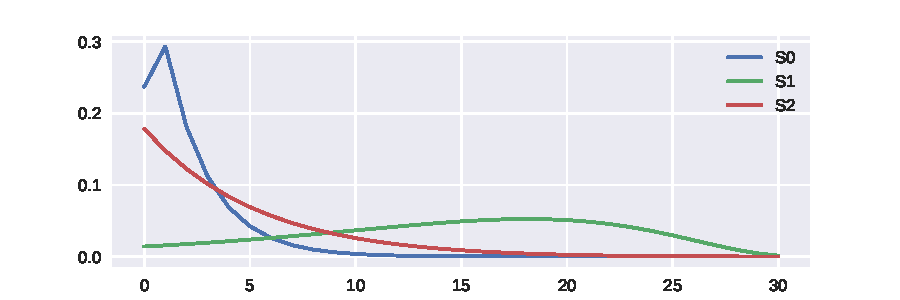
\includegraphics{mda_mass}

  \end{solution}
\end{exercise}





\Closesolutionfile{hint}
\Closesolutionfile{ans}

\opt{solutionfiles}{
\subsection*{Hints}
\input{hint}
\subsection*{Solutions}
\input{ans}
}
\clearpage


\chapter{Extra Topics}
%\input{todo/extra_notes.tex}

%\includequestions[random=2]{single_station}

\chapter{To Do}
\label{cha:extra-topics}

%\input{tex_files/mg1_markov_chain.tex}
%\input{tex_files/open_move_batches.tex}


%\chapter{Hints}
%\addcontentsline{toc}{chapter}{Hints}
% \fancyhead{} % clear all header fields
% \fancyhead[LO, LE]{HINTS}
%\printquestionhints

%\chapter{Solutions}
%\addcontentsline{toc}{chapter}{Solutions}
% \fancyhead{} % clear all header fields
% \fancyhead[LO, LE]{SOLUTIONS}
%\printsolutions

\chapter*{Notation}
%\addcontentsline{toc}{chapter}{Notation}
% \label{sec:notation}
% \begin{align*}
  a_n &= \text{Number of arrivals in the $n$th period} \\
  A(t) &= \text{Number of arrivals in $[0,t]$} \\
  A_k &= \text{Arrival time of $k$th job} \\
  c_n &= \text{Service/production capacity in the $n$th period} \\
  d_n &= \text{Number of departures in the $n$th period} \\
  c &= \text{Number of servers} \\
  C_a^2 &= \text{Squared coefficient of variation of the interarrival times} \\
  C_s^2 &= \text{Squared coefficient of variation of the service times} \\
  D(t) &= \text{Number of departures in $[0,t]$} \\
  D_Q(t) &= \text{Number of customers/jobs that departed from the queue in $[0,t]$} \\
  D_n &= \text{Departure time of $n$th job} \\
  D_{Q,n} &= \text{Departure time of the queue of $n$th job} \\
  F &= \text{Distribution of the service time of a job} \\
  L(t) &= \text{Number of customers/jobs in the system at time $t$} \\
  Q(t) &= \text{Number of customers/jobs in queue at time $t$} \\
  L_S(t) &= \text{Number of customers/jobs in service at time $t$} \\
  \E L &= \text{Long run (time) average of the number of jobs in the system} \\
  \E Q &= \text{Long run (time) average of the number of jobs in queue} \\
  \E L_S &= \text{Long run (time) average of the number of jobs in service} \\
  N(t) &= \text{Number of events in $[0,t]$} \\
  N(s,t) &= \text{Number of events in $(s,t]$} \\
  p(n)  &= \text{Long-run time average that the system contains $n$ jobs} \\
  Q_n &= \text{Queue length as seen by the $n$th job, or at the \textit{end} of the $n$th period} \\
  S_k &= \text{Service time required by the $k$th job} \\
  S(t) &= \text{Total service time available in $[0,t]$} \\
  S &= \text{generic service time of a job} \\
  t &= \text{time} \\
  W_n &= \text{time in the system of $n$th job} \\
  W_{Q,n} &= \text{time in the queue of $n$th job} \\
  \E W &= \text{sample average of the sojourn time} \\
  \E W_Q &= \text{sample average of the time in queue} \\
  X_k &= \text{inter-arrival time between job $k-1$ and job  $k$} \\
  X &= \text{generic interarrival time between two consecutive jobs} \\
  \gamma &= \text{departure rate} \\
  \lambda &= \text{arrival rate} \\
  \mu &= \text{service rate} \\
  \pi(n)  &= \text{Stationary probability that an arrival sees $n$ jobs in the system} \\
  \rho &= \text{Load on the system} \\
\end{align*}


\chapter*{Formula Sheet}
%\addcontentsline{toc}{chapter}{Formula Sheet}
%\begin{flalign*}
&\rho = \lambda \frac{\E S}{c} \\
&\E{W_Q} = \frac{C_a^2 + C_s^2}{2} \frac{\rho^{\sqrt{2(c+1)}-1}}{c(1-\rho)} \E S  \\
&\text{Batching: } C_{sB}^2 = \frac{B \V{S_0}+\V{T}}{(B\E{S_0}+\E{T})^2} \\ 
&\text{Nonpreemptive: } \V{S} = \V{S_0} + \frac{\V{T}}{B} + \frac{B -1}{B^2}(\E{T})^2\\
&\text{Preemptive: } A = \frac{m_f}{m_r+m_f}, C_s^2 = C_0^2 + 2A(1-A)\frac{m_r}{\E{S_0}}, \\
%& \sigma_s^2 = \sigma_0^2 + \sigma_r^2 f_r + f_r(1-f_r)(\E{S_r})^2 
\\
& C_{di}^2 = 1 + (1-\rho_i^2)(C_{ai}^2 - 1) + \frac{\rho_i^2}{\sqrt{c_i}}(C_{si}^2-1) 
 &\quad 
%C_{ij}^2 = P_{ij}C_{di}^2 + 1 - P_{ij}
\\
& f_i(n_i) = 
            \begin{cases}
              G(i)^{-1} (c_i\rho_i)^{n_i}(n_i!)^{-1}, &\text{ if } n_i < c_i, \\ 
              G(i)^{-1} c_i^{c_i}\rho_i^{n_i}(c_i!)^{-1}, &\text{ if } n_i \geq c_i \\ 
            \end{cases} 
\quad \text{with } G(i) = \sum_{n=0}^{c_i-1} \frac{(c_i\rho_i)^n}{n!} + \frac{(c_i\rho_i)^{c_i}}{c_i!}\frac{1}{1-\rho_i} \\
& \E{L_i} = \frac{(c_i\rho_i)^{c_i}}{c_i!G(i)}\frac{\rho_i}{(1-\rho_i)^2} + c_i \rho_i &\quad
% C_{si}^2 = \max\{C_{si}^2, 0.2\} 
\\
%& Q_{ij} = \frac{\lambda_{ij}}{\lambda_j}, i=0\ldots M, j=1\ldots M &\quad C_{aj}^2 = w_j\sum_{i=0}^M Q_{ij}C_{ij}^2 + 1 - w_j \\
%& w_j = (1+4(1-\rho_j)^2(v_j-1))^{-1} &\quad 
% v_j = \left(\sum_{i=0}^M Q_{ij}^2\right)^{-1}, \, j=1,\ldots, M,\\
& f_{i}(n_i) = \frac{1}{\Pi_{k=1}^{n_i} \min\{k, c_i\}}\left(\frac{V_i}{\mu_i}\right)^{n_i}, i=0\ldots M \\
& V_i = (V P)_i = \sum_{j=0}^M V_j P_{ji}\\
%& G(m,n) = \sum_{k=0}^n f_m(k) G(m-1, n-k) &\quad  G(m,0) = 1, G(0,n) = \mu_0^{-n}, \\
%& \E{W_j(n)} = \E{L_j(n-1) + 1} \E{S_j} &\quad \E{L_j(n)} = \TH_j(n) \E{W_j(n)} \\
%& \TH_0(n) = \frac{n}{\sum_{j=0}^M V_j \E{W_j(n)}}  &\quad  \TH_j(n) = V_j \TH_0(n) \\
%&  p_j(0|0) = 1  &\quad \E{W_j(n)} = \sum_{k=c_j}^{n-1} \frac{k-c_j+1}{c_j \mu_j} p_j(k|n-1) + \frac{1}{\mu_j} \\
%& p_j(k|n) = \frac{\TH_j(n)}{\mu_j \min\{c_j,k\}} p_j(k-1|n-1), k=1\ldots N &\quad p_j(0|n) = 1 - \sum_{k=1}^n p_j(k|n).
\end{flalign*}




\bibliographystyle{plainnat}
\bibliography{biblio_nicky}
\end{document}

%%% Local Variables:
%%% mode: latex
%%% TeX-master: t
%%% End:
